% Options for packages loaded elsewhere
\PassOptionsToPackage{unicode}{hyperref}
\PassOptionsToPackage{hyphens}{url}
%
\documentclass[
]{book}
\usepackage{lmodern}
\usepackage{amssymb,amsmath}
\usepackage{ifxetex,ifluatex}
\ifnum 0\ifxetex 1\fi\ifluatex 1\fi=0 % if pdftex
  \usepackage[T1]{fontenc}
  \usepackage[utf8]{inputenc}
  \usepackage{textcomp} % provide euro and other symbols
\else % if luatex or xetex
  \usepackage{unicode-math}
  \defaultfontfeatures{Scale=MatchLowercase}
  \defaultfontfeatures[\rmfamily]{Ligatures=TeX,Scale=1}
\fi
% Use upquote if available, for straight quotes in verbatim environments
\IfFileExists{upquote.sty}{\usepackage{upquote}}{}
\IfFileExists{microtype.sty}{% use microtype if available
  \usepackage[]{microtype}
  \UseMicrotypeSet[protrusion]{basicmath} % disable protrusion for tt fonts
}{}
\makeatletter
\@ifundefined{KOMAClassName}{% if non-KOMA class
  \IfFileExists{parskip.sty}{%
    \usepackage{parskip}
  }{% else
    \setlength{\parindent}{0pt}
    \setlength{\parskip}{6pt plus 2pt minus 1pt}}
}{% if KOMA class
  \KOMAoptions{parskip=half}}
\makeatother
\usepackage{xcolor}
\IfFileExists{xurl.sty}{\usepackage{xurl}}{} % add URL line breaks if available
\IfFileExists{bookmark.sty}{\usepackage{bookmark}}{\usepackage{hyperref}}
\hypersetup{
  pdftitle={EPI 563: Spatial Epidemiology, Fall 2020},
  pdfauthor={Michael Kramer},
  hidelinks,
  pdfcreator={LaTeX via pandoc}}
\urlstyle{same} % disable monospaced font for URLs
\usepackage{listings}
\newcommand{\passthrough}[1]{#1}
\lstset{defaultdialect=[5.3]Lua}
\lstset{defaultdialect=[x86masm]Assembler}
\usepackage{longtable,booktabs}
% Correct order of tables after \paragraph or \subparagraph
\usepackage{etoolbox}
\makeatletter
\patchcmd\longtable{\par}{\if@noskipsec\mbox{}\fi\par}{}{}
\makeatother
% Allow footnotes in longtable head/foot
\IfFileExists{footnotehyper.sty}{\usepackage{footnotehyper}}{\usepackage{footnote}}
\makesavenoteenv{longtable}
\usepackage{graphicx}
\makeatletter
\def\maxwidth{\ifdim\Gin@nat@width>\linewidth\linewidth\else\Gin@nat@width\fi}
\def\maxheight{\ifdim\Gin@nat@height>\textheight\textheight\else\Gin@nat@height\fi}
\makeatother
% Scale images if necessary, so that they will not overflow the page
% margins by default, and it is still possible to overwrite the defaults
% using explicit options in \includegraphics[width, height, ...]{}
\setkeys{Gin}{width=\maxwidth,height=\maxheight,keepaspectratio}
% Set default figure placement to htbp
\makeatletter
\def\fps@figure{htbp}
\makeatother
\setlength{\emergencystretch}{3em} % prevent overfull lines
\providecommand{\tightlist}{%
  \setlength{\itemsep}{0pt}\setlength{\parskip}{0pt}}
\setcounter{secnumdepth}{5}
\usepackage{booktabs}
\usepackage{amsthm}
\makeatletter
\def\thm@space@setup{%
  \thm@preskip=8pt plus 2pt minus 4pt
  \thm@postskip=\thm@preskip
}
\makeatother


% create callout boxes:
\newenvironment{rmdblock}[1]
  {%\begin{shaded*}
  \begin{itemize}
  \renewcommand{\labelitemi}{
    \raisebox{-.7\height}[0pt][0pt]{
      {\setkeys{Gin}{width=3em,keepaspectratio}\includegraphics{images/#1}}
    }
  }
  \item
  }
  {
  \end{itemize}
  %\end{shaded*}
  }
\newenvironment{rmdnote}
  {\begin{rmdblock}{note}}
  {\end{rmdblock}}
\newenvironment{rmdtip}
  {\begin{rmdblock}{tip}}
  {\end{rmdblock}}
\newenvironment{rmdwarning}
  {\begin{rmdblock}{warning}}
  {\end{rmdblock}}
\newenvironment{rmdcaution}
  {\begin{rmdblock}{caution}}
  {\end{rmdblock}}
\newenvironment{rmdtask}
  {\begin{rmdblock}{task}}
  {\end{rmdblock}}
  \newenvironment{rmdactivity}
  {\begin{rmdblock}{activity}}
  {\end{rmdblock}}


\lstset{
  breaklines=true
}
\usepackage{array}
\usepackage{caption}
\usepackage{graphicx}
\usepackage{siunitx}
\usepackage{ulem}
\usepackage{colortbl}
\usepackage{multirow}
\usepackage{hhline}
\usepackage{calc}
\usepackage{tabularx}
\usepackage{threeparttable}
\usepackage{wrapfig}
\usepackage{adjustbox}
\usepackage[]{natbib}
\bibliographystyle{apalike}

\title{EPI 563: Spatial Epidemiology, Fall 2020}
\author{Michael Kramer}
\date{Last updated: 2020-11-11}

\begin{document}
\maketitle

{
\setcounter{tocdepth}{1}
\tableofcontents
}
\hypertarget{how-to-use-this-ebook}{%
\chapter*{How to use this eBook}\label{how-to-use-this-ebook}}
\addcontentsline{toc}{chapter}{How to use this eBook}

\begin{center}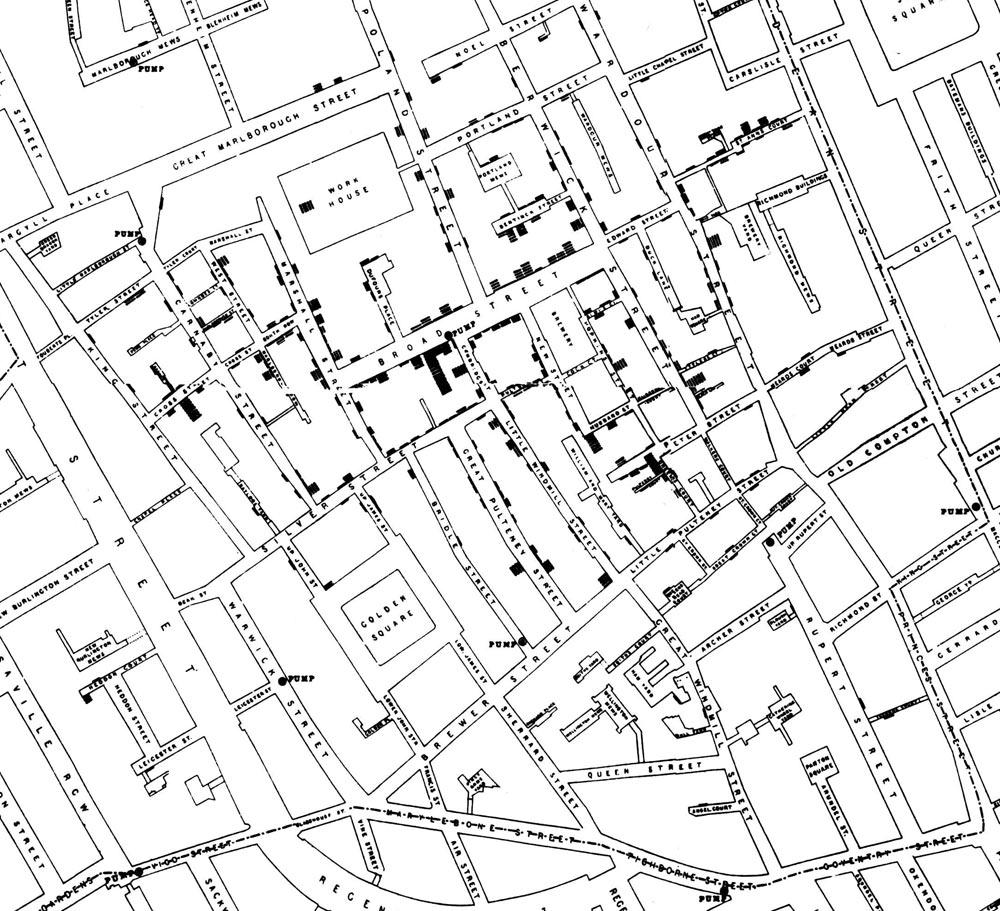
\includegraphics[width=0.5\linewidth]{images/John-Snows-cholera-map-of-009} \end{center}

Welcome to \emph{Concepts \& Applications in Spatial Epidemiology (EPI 563)}! This eBook is one of several sources of information and support for your progress through the semester. For an overview of the course, expectations, learning objectives, assignments, and grading, please review the full course syllabus on Canvas. This eBook serves to provide a \emph{`jumping off point'} for the content to be covered each week. Specifically, the content herein will introduce key themes, new vocabulary, and provide some additional detail that is complementary to the \emph{asynchronous} (pre-recorded) video lectures, and foundational to the \emph{synchronous} (in class) work.

\hypertarget{strategy-for-using-this-ebook}{%
\section*{Strategy for using this eBook}\label{strategy-for-using-this-ebook}}
\addcontentsline{toc}{section}{Strategy for using this eBook}

There is a separate \emph{module} or \emph{chapter} for each week's content. In general, the content within each week's section is divided into two sections focusing on \textbf{spatial thinking} and \textbf{spatial analysis}. This dichotomy does not always hold, but in broad terms you can expect these sections to be more specific to content in class on \emph{Tuesday} versus \emph{Thursday} respectively.

\begin{itemize}
\tightlist
\item
  \emph{Spatial thinking for epidemiology}: This section introduces vocabulary, concepts, and themes that are important to the incorporation of spatialized or geo-referenced data into epidemiologic work. At a minimum, plan to read this content prior to class Tuesday, although you will likely benefit from reading both sections before Tuesday.
\item
  \emph{Spatial analysis for epidemiology}: This section is more focused on data management, visualization, spatial statistics, and interpretation. This content is relevant for our work together on Tuesday's, but is essential for successful work in the Thursday lab activities.
\end{itemize}

Please note that I will be continually updating the eBook throughout the semester, so if you choose to download, please double-check the \textbf{Last updated} date to be sure you have the most recent version.


\includegraphics{images/by-nc-sa.png}\\
This eBook is licensed under the \href{http://creativecommons.org/licenses/by-nc-sa/4.0/}{Creative Commons Attribution-NonCommercial-ShareAlike 4.0 International License}.

\hypertarget{part-getting-ready}{%
\part{Getting ready\ldots{}}\label{part-getting-ready}}

\hypertarget{software-installation}{%
\chapter*{Software installation}\label{software-installation}}
\addcontentsline{toc}{chapter}{Software installation}

The information in this module follow on the pre-class video on setting up \passthrough{\lstinline!R!} and \passthrough{\lstinline!RStudio!} on your computer.

\hypertarget{installing-r-on-your-computer}{%
\section*{\texorpdfstring{Installing \texttt{R} on your computer}{Installing R on your computer}}\label{installing-r-on-your-computer}}
\addcontentsline{toc}{section}{Installing \texttt{R} on your computer}

As of August 2020, the most up-to-date version of \passthrough{\lstinline!R!} is 4.0.2. The \emph{R Project for Statistical Computing} are continually working to update and improve \passthrough{\lstinline!R!}, and as a result there are new versions 1-2 times per year.

If you already have \passthrough{\lstinline!R!} installed, you can open the console and check your current version by doing this: \passthrough{\lstinline!R.Version()$version.string!}

If you do not have \passthrough{\lstinline!R!} or have an older version than 4.0 you can install \passthrough{\lstinline!R!} by going to the \passthrough{\lstinline!R!} repository: \url{https://www.r-project.org/}. Note that there are many `mirrors' or servers where the software is stored. Generally it is wise to select one that is geographically close to you, although any should work in theory. One mirror that is relatively close to Atlanta is here: \url{http://archive.linux.duke.edu/cran/}

\hypertarget{installing-rstudio-on-your-computer}{%
\section*{Installing RStudio on your computer}\label{installing-rstudio-on-your-computer}}
\addcontentsline{toc}{section}{Installing RStudio on your computer}

The current version of RStudio 1.3.1056. If you do not have RStudio or have a version older than 1.2 please install/update.

\textbf{TO INSTALL}: go to \url{https://www.rstudio.com/products/rstudio/download/}

\textbf{TO UPDATE}: Open RStudio and go to Help Menu and choose `Check for Updates'

\hypertarget{installing-packages-for-this-course}{%
\chapter*{Installing packages for this course}\label{installing-packages-for-this-course}}
\addcontentsline{toc}{chapter}{Installing packages for this course}

While base \passthrough{\lstinline!R!} has a great deal of essential functionality, most of the power of \passthrough{\lstinline!R!} comes from the rapidly growing list of user-created and contributed `packages'. A package is simply a bundle of functions and tools, sometimes also including example datasets, basic documentation, and even tutorial `vignettes'. You can see all the official \passthrough{\lstinline!R!} packages by going here: \url{https://cran.r-project.org/web/packages/}.

The most common way to install package in \passthrough{\lstinline!R!} is with the \passthrough{\lstinline!install.packages()!} command. For instance to install the package \passthrough{\lstinline!ggplot2!} you do this:

\passthrough{\lstinline!install.packages("ggplot2")!}

Notice that for \passthrough{\lstinline!install.packages()!} you need quotes around the package name. Remember that you only need to install a package once (although you may have to update packages occasionally -- see the green Update button in the Packages tab in R Studio). When you want to actually \emph{use} a package (for example \passthrough{\lstinline!ggplot2!}) you call it like this:

\passthrough{\lstinline!library(ggplot2)!}

Notice that for the \passthrough{\lstinline!library()!} function you \textbf{do not} need quotes around the package name (unlike the \passthrough{\lstinline!install.packages()!} above). If your call to \passthrough{\lstinline!library()!} is working, nothing visible happens. However if you see errors, they might be because your package is out of date (and thus needs to be updated/reinstalled), or because some important \emph{dependencies} are missing. Dependencies are other packages on which this package depends. Typically these are installed by default, but sometimes something is missing. If so, simply install the missing package and then try calling \passthrough{\lstinline!library(ggplot2)!} again.

While \textbf{most} packages can be installed as mentioned above (e.g.~using \passthrough{\lstinline!install.packages()!}), there are instances where an installation requires additional \emph{tools}, for instance to install from source or from github. Luckily there is a package for that! It is called \passthrough{\lstinline!Rtools!}, and you should install that \textbf{before} you install the packages below.

\begin{rmdcaution}
As you submit each installation request, note the output. If you get a warning that says installation was not possible because you are missing a package \emph{`namespace'}, that suggests you are missing a dependency. Try installing the pacakge mentioned in the error. If you have trouble, reach out to the TA's!
\end{rmdcaution}

\hypertarget{installing-rtools40}{%
\section*{\texorpdfstring{Installing \texttt{Rtools40}}{Installing Rtools40}}\label{installing-rtools40}}
\addcontentsline{toc}{section}{Installing \texttt{Rtools40}}

If your laptop uses a Windows operating system, you may need \passthrough{\lstinline!Rtools40!} installed. This is a supplemental package that resides \emph{outside} of \passthrough{\lstinline!R!} but is needed to install some packages from source code. However it appears that if you have a MacOS, these tools are already built-in. So you \emph{do not need \passthrough{\lstinline!Rtools40!}} for Mac.

If you are running Windows, navigate to this website: \url{https://cran.r-project.org/bin/windows/Rtools/} and follow the instructions specific to your operating system.

\hypertarget{installing-packages-used-for-general-data-science}{%
\section*{Installing packages used for general data science}\label{installing-packages-used-for-general-data-science}}
\addcontentsline{toc}{section}{Installing packages used for general data science}

For the rest of this page, copy and paste the provided code in order to install packages necessary for this course. Notice if you hover to the right of a code-chunk in the html version of the eBook, you will see a \emph{copy} icon for quick copying and pasting.

These packages will support some of our general work in \passthrough{\lstinline!R!}, including working with \passthrough{\lstinline!RMarkdown!} and R Notebooks, as well as data manipulation tools from the \passthrough{\lstinline!tidyverse!}. You can learn more about the \passthrough{\lstinline!tidyverse!} here: \url{https://tidyverse.tidyverse.org/}. The \passthrough{\lstinline!tidyverse!} is actually a collection of data science tools including the visualization/plotting package \passthrough{\lstinline!ggplot2!} and the data manipulation package \passthrough{\lstinline!dplyr!}. For that reason, when you \passthrough{\lstinline!install.packages('tidyverse')!} below, you are actually installing \emph{multiple} packages! The packages \passthrough{\lstinline!tinytex!}, \passthrough{\lstinline!rmarkdown!}, and \passthrough{\lstinline!knitr!} are all necessary for creating \passthrough{\lstinline!R!} Notebooks, which is the format by which many assignments will be submitted.

\begin{lstlisting}[language=R]
install.packages('tidyverse')   
install.packages(c('tinytex', 'rmarkdown', 'knitr')) 
tinytex::install_tinytex()  
# this function installs the tinytex LaTex on your
#  computer which is necessary for rendering (creating) PDF's 
\end{lstlisting}

\hypertarget{installing-packages-use-for-geographic-data}{%
\section*{Installing packages use for geographic data}\label{installing-packages-use-for-geographic-data}}
\addcontentsline{toc}{section}{Installing packages use for geographic data}

There are many ways to get the data we want for spatial epidemiology into \passthrough{\lstinline!R!}. Because we often (but don't always) use census geographies as aggregating units, and census populations as denominators, the following packages will be useful. They are designed to quickly extract both geographic boundary files (e.g.~\emph{`shapefiles'}) as well as attribute data from the US Census website via an API. \textbf{NOTE}: For these to work you have to request a free Census API key. Notice the \passthrough{\lstinline!help()!} function below to get instructions on how to do this.

\begin{lstlisting}[language=R]
install.packages(c('tidycensus','tigris')) 

help('census_api_key','tidycensus')
\end{lstlisting}

\hypertarget{installing-packages-used-for-spatial-data-manipulation-visualization}{%
\section*{Installing packages used for spatial data manipulation \& visualization}\label{installing-packages-used-for-spatial-data-manipulation-visualization}}
\addcontentsline{toc}{section}{Installing packages used for spatial data manipulation \& visualization}

This section installs a set of tools specific to our goals of importing, exporting, manipulating, visualizing, and analyzing spatial data. The first line of packages have functions for defining, importing, exporting, and manipulating spatial data. The second line has some tools we will use for visualizing spatial data (e.g.~making maps!).

\begin{lstlisting}[language=R]
install.packages(c('sp', 'sf', 'rgdal', 'rgeos', 'maptools', 'OpenStreetMap'))  
install.packages(c('tmap', 'tmaptools', 'ggmap', 'shinyjs', 'shiny', 'micromap')) 
\end{lstlisting}

\hypertarget{installing-packages-used-for-spatial-analysis}{%
\section*{Installing packages used for spatial analysis}\label{installing-packages-used-for-spatial-analysis}}
\addcontentsline{toc}{section}{Installing packages used for spatial analysis}

Finally these are packages specifically to spatial analysis tasks we'll carry out.

\begin{lstlisting}[language=R]
install.packages(c('spdep', 'CARBayes', 'sparr', 'spatialreg', 'scanstatistics'))
install.packages(c('GWmodel', 'spgwr') )
\end{lstlisting}

\hypertarget{part-weekly-modules}{%
\part{Weekly Modules}\label{part-weekly-modules}}

\hypertarget{locating-spatial-epidemiology}{%
\chapter{Locating Spatial Epidemiology}\label{locating-spatial-epidemiology}}

\hypertarget{getting-ready}{%
\section{Getting Ready}\label{getting-ready}}

\hypertarget{learning-objectives}{%
\subsection{Learning objectives}\label{learning-objectives}}

 
  \providecommand{\huxb}[2]{\arrayrulecolor[RGB]{#1}\global\arrayrulewidth=#2pt}
  \providecommand{\huxvb}[2]{\color[RGB]{#1}\vrule width #2pt}
  \providecommand{\huxtpad}[1]{\rule{0pt}{#1}}
  \providecommand{\huxbpad}[1]{\rule[-#1]{0pt}{#1}}

\begin{table}[ht]
\begin{centerbox}
\begin{threeparttable}
\captionsetup{justification=centering,singlelinecheck=off}
\caption{\label{tab:learning-ob} Learning objectives by weekly module}
 \setlength{\tabcolsep}{0pt}
\begin{tabularx}{1\textwidth}{p{1\textwidth}}


\hhline{>{\huxb{255, 255, 255}{1}}-}
\arrayrulecolor{black}

\multicolumn{1}{!{\huxvb{255, 255, 255}{1}}p{1\textwidth}!{\huxvb{255, 255, 255}{1}}}{\cellcolor[RGB]{208, 211, 212}\hspace{6pt}\parbox[b]{1\textwidth-6pt-6pt}{\huxtpad{2pt + 1em}\raggedright \textbf{After this module you should be able to…}\huxbpad{2pt}}} \tabularnewline[-0.5pt]


\hhline{>{\huxb{255, 255, 255}{1}}-}
\arrayrulecolor{black}

\multicolumn{1}{!{\huxvb{255, 255, 255}{1}}p{1\textwidth}!{\huxvb{255, 255, 255}{1}}}{\cellcolor[RGB]{250, 229, 211}\hspace{6pt}\parbox[b]{1\textwidth-6pt-6pt}{\huxtpad{2pt + 1em}\raggedright Explain the potential role of spatial analysis for epidemiologic thinking and practice.\huxbpad{2pt}}} \tabularnewline[-0.5pt]


\hhline{>{\huxb{255, 255, 255}{1}}-}
\arrayrulecolor{black}

\multicolumn{1}{!{\huxvb{255, 255, 255}{1}}p{1\textwidth}!{\huxvb{255, 255, 255}{1}}}{\cellcolor[RGB]{245, 203, 167}\hspace{6pt}\parbox[b]{1\textwidth-6pt-6pt}{\huxtpad{2pt + 1em}\raggedright Produce simple thematic maps of epidemiologic data in R.\huxbpad{2pt}}} \tabularnewline[-0.5pt]


\hhline{>{\huxb{255, 255, 255}{1}}-}
\arrayrulecolor{black}
\end{tabularx}
\end{threeparttable}\par\end{centerbox}

\end{table}
 

\hypertarget{additional-resources}{%
\subsection{Additional Resources}\label{additional-resources}}

\begin{itemize}
\tightlist
\item
  \href{https://geocompr.robinlovelace.net/}{Geocompution with R} by Robin Lovelace. This will be a recurring `additional resource' as it provides lots of useful insight and strategy for working with spatial data in \passthrough{\lstinline!R!}. I encourage you to browse it quickly now, but return often when you have qusetiona about how to handle geogrpahic data (especially of class \passthrough{\lstinline!sf!}) in \passthrough{\lstinline!R!}.
\item
  \href{https://bookdown.org/agrogankaylor/quick-intro-to-ggplot2/quick-intro-to-ggplot2.html}{A basic introduction to the \passthrough{\lstinline!ggplot2!} package}. This is just one of dozens of great online resources introducing the \emph{grammar of graphics} approach to plotting in \passthrough{\lstinline!R!}.
\item
  \href{https://tlorusso.github.io/geodata_workshop/tmap_package\#:~:text=The\%20tmap\%20package\%20is\%20a,as\%20choropleths\%20and\%20bubble\%20maps.}{A basic introduction to the \passthrough{\lstinline!tmap!} package} This is also only one of many introductions to the \passthrough{\lstinline!tmap!} mapping package. \passthrough{\lstinline!tmap!} builds on the \emph{grammar of graphics} philosophy of \passthrough{\lstinline!ggplot2!}, but brings a lot of tools useful for thematic mapping!
\end{itemize}

\hypertarget{important-vocabulary}{%
\subsection{Important Vocabulary}\label{important-vocabulary}}

 
  \providecommand{\huxb}[2]{\arrayrulecolor[RGB]{#1}\global\arrayrulewidth=#2pt}
  \providecommand{\huxvb}[2]{\color[RGB]{#1}\vrule width #2pt}
  \providecommand{\huxtpad}[1]{\rule{0pt}{#1}}
  \providecommand{\huxbpad}[1]{\rule[-#1]{0pt}{#1}}

\begin{table}[ht]
\begin{centerbox}
\begin{threeparttable}
\captionsetup{justification=centering,singlelinecheck=off}
\caption{\label{tab:unnamed-chunk-9} Vocabulary for Week 1}
 \setlength{\tabcolsep}{0pt}
\begin{tabularx}{0.9\textwidth}{p{0.45\textwidth} p{0.45\textwidth}}


\hhline{>{\huxb{255, 255, 255}{1}}->{\huxb{255, 255, 255}{1}}-}
\arrayrulecolor{black}

\multicolumn{1}{!{\huxvb{255, 255, 255}{1}}p{0.45\textwidth}!{\huxvb{255, 255, 255}{1}}}{\cellcolor[RGB]{84, 153, 199}\hspace{6pt}\parbox[b]{0.45\textwidth-6pt-2pt}{\huxtpad{2pt + 1em}\raggedright \textbf{\textcolor[RGB]{255, 255, 255}{Term}}\huxbpad{2pt}}} &
\multicolumn{1}{p{0.45\textwidth}!{\huxvb{255, 255, 255}{1}}}{\cellcolor[RGB]{84, 153, 199}\hspace{2pt}\parbox[b]{0.45\textwidth-2pt-6pt}{\huxtpad{2pt + 1em}\raggedright \textbf{\textcolor[RGB]{255, 255, 255}{Definition}}\huxbpad{2pt}}} \tabularnewline[-0.5pt]


\hhline{>{\huxb{255, 255, 255}{1}}->{\huxb{255, 255, 255}{1}}-}
\arrayrulecolor{black}

\multicolumn{1}{!{\huxvb{255, 255, 255}{1}}p{0.45\textwidth}!{\huxvb{255, 255, 255}{1}}}{\cellcolor[RGB]{212, 230, 241}\hspace{6pt}\parbox[b]{0.45\textwidth-6pt-2pt}{\huxtpad{2pt + 1em}\raggedright \textbf{Data, attribute}\huxbpad{2pt}}} &
\multicolumn{1}{p{0.45\textwidth}!{\huxvb{255, 255, 255}{1}}}{\cellcolor[RGB]{212, 230, 241}\hspace{2pt}\parbox[b]{0.45\textwidth-2pt-6pt}{\huxtpad{2pt + 1em}\raggedright Nonspatial information about a geographic feature in a GIS, usually stored in a table and linked to the feature by a unique identifier. For example, attributes of a county might include the population size, density, and birth rate for the resident population\huxbpad{2pt}}} \tabularnewline[-0.5pt]


\hhline{>{\huxb{255, 255, 255}{1}}->{\huxb{255, 255, 255}{1}}-}
\arrayrulecolor{black}

\multicolumn{1}{!{\huxvb{255, 255, 255}{1}}p{0.45\textwidth}!{\huxvb{255, 255, 255}{1}}}{\cellcolor[RGB]{169, 204, 227}\hspace{6pt}\parbox[b]{0.45\textwidth-6pt-2pt}{\huxtpad{2pt + 1em}\raggedright \textbf{Data, geometry}\huxbpad{2pt}}} &
\multicolumn{1}{p{0.45\textwidth}!{\huxvb{255, 255, 255}{1}}}{\cellcolor[RGB]{169, 204, 227}\hspace{2pt}\parbox[b]{0.45\textwidth-2pt-6pt}{\huxtpad{2pt + 1em}\raggedright Spatial information about a geogrpahic feature. This could include the x, y coordinates for points or for vertices of lines or polygons, or the cell coordinates for raster data\huxbpad{2pt}}} \tabularnewline[-0.5pt]


\hhline{>{\huxb{255, 255, 255}{1}}->{\huxb{255, 255, 255}{1}}-}
\arrayrulecolor{black}

\multicolumn{1}{!{\huxvb{255, 255, 255}{1}}p{0.45\textwidth}!{\huxvb{255, 255, 255}{1}}}{\cellcolor[RGB]{212, 230, 241}\hspace{6pt}\parbox[b]{0.45\textwidth-6pt-2pt}{\huxtpad{2pt + 1em}\raggedright \textbf{Datum}\huxbpad{2pt}}} &
\multicolumn{1}{p{0.45\textwidth}!{\huxvb{255, 255, 255}{1}}}{\cellcolor[RGB]{212, 230, 241}\hspace{2pt}\parbox[b]{0.45\textwidth-2pt-6pt}{\huxtpad{2pt + 1em}\raggedright The reference specifications of a measurement system, usually a system of coordinate positions on a surface (a horizontal datum) or heights above or below a surface (a vertical datum)\huxbpad{2pt}}} \tabularnewline[-0.5pt]


\hhline{>{\huxb{255, 255, 255}{1}}->{\huxb{255, 255, 255}{1}}-}
\arrayrulecolor{black}

\multicolumn{1}{!{\huxvb{255, 255, 255}{1}}p{0.45\textwidth}!{\huxvb{255, 255, 255}{1}}}{\cellcolor[RGB]{169, 204, 227}\hspace{6pt}\parbox[b]{0.45\textwidth-6pt-2pt}{\huxtpad{2pt + 1em}\raggedright \textbf{Geographic coordinate system}\huxbpad{2pt}}} &
\multicolumn{1}{p{0.45\textwidth}!{\huxvb{255, 255, 255}{1}}}{\cellcolor[RGB]{169, 204, 227}\hspace{2pt}\parbox[b]{0.45\textwidth-2pt-6pt}{\huxtpad{2pt + 1em}\raggedright A reference system that uses latitude and longitude to define the locations of points on the surface of a sphere or spheroid. A geographic coordinate system definition includes a datum, prime meridian, and angular unit\huxbpad{2pt}}} \tabularnewline[-0.5pt]


\hhline{>{\huxb{255, 255, 255}{1}}->{\huxb{255, 255, 255}{1}}-}
\arrayrulecolor{black}

\multicolumn{1}{!{\huxvb{255, 255, 255}{1}}p{0.45\textwidth}!{\huxvb{255, 255, 255}{1}}}{\cellcolor[RGB]{212, 230, 241}\hspace{6pt}\parbox[b]{0.45\textwidth-6pt-2pt}{\huxtpad{2pt + 1em}\raggedright \textbf{Projection}\huxbpad{2pt}}} &
\multicolumn{1}{p{0.45\textwidth}!{\huxvb{255, 255, 255}{1}}}{\cellcolor[RGB]{212, 230, 241}\hspace{2pt}\parbox[b]{0.45\textwidth-2pt-6pt}{\huxtpad{2pt + 1em}\raggedright A method by which the curved surface of the earth is portrayed on a flat surface. This generally requires a systematic mathematical transformation of the earth's graticule of lines of longitude and latitude onto a plane. Some projections can be visualized as a transparent globe with a light bulb at its center (though not all projections emanate from the globe's center) casting lines of latitude and longitude onto a sheet of paper. Generally, the paper is either flat and placed tangent to the globe (a planar or azimuthal projection) or formed into a cone or cylinder and placed over the globe (cylindrical and conical projections). Every map projection distorts distance, area, shape, direction, or some combination thereof\huxbpad{2pt}}} \tabularnewline[-0.5pt]


\hhline{>{\huxb{255, 255, 255}{1}}->{\huxb{255, 255, 255}{1}}-}
\arrayrulecolor{black}

\multicolumn{1}{!{\huxvb{255, 255, 255}{1}}p{0.45\textwidth}!{\huxvb{255, 255, 255}{1}}}{\cellcolor[RGB]{169, 204, 227}\hspace{6pt}\parbox[b]{0.45\textwidth-6pt-2pt}{\huxtpad{2pt + 1em}\raggedright \textbf{Spatial data model: raster}\huxbpad{2pt}}} &
\multicolumn{1}{p{0.45\textwidth}!{\huxvb{255, 255, 255}{1}}}{\cellcolor[RGB]{169, 204, 227}\hspace{2pt}\parbox[b]{0.45\textwidth-2pt-6pt}{\huxtpad{2pt + 1em}\raggedright A spatial data model that defines space as an array of equally sized cells arranged in rows and columns, and composed of single or multiple bands. Each cell contains an attribute value and location coordinates. Unlike a vector structure, which stores coordinates explicitly, raster coordinates are contained in the ordering of the matrix. Groups of cells that share the same value represent the same type of geographic feature (see Figure below)\huxbpad{2pt}}} \tabularnewline[-0.5pt]


\hhline{>{\huxb{255, 255, 255}{1}}->{\huxb{255, 255, 255}{1}}-}
\arrayrulecolor{black}

\multicolumn{1}{!{\huxvb{255, 255, 255}{1}}p{0.45\textwidth}!{\huxvb{255, 255, 255}{1}}}{\cellcolor[RGB]{212, 230, 241}\hspace{6pt}\parbox[b]{0.45\textwidth-6pt-2pt}{\huxtpad{2pt + 1em}\raggedright \textbf{Spatial data model: vector}\huxbpad{2pt}}} &
\multicolumn{1}{p{0.45\textwidth}!{\huxvb{255, 255, 255}{1}}}{\cellcolor[RGB]{212, 230, 241}\hspace{2pt}\parbox[b]{0.45\textwidth-2pt-6pt}{\huxtpad{2pt + 1em}\raggedright A coordinate-based data model that represents geographic features as points, lines, and polygons. Each point feature is represented as a single coordinate pair, while line and polygon features are represented as ordered lists of vertices. Attributes are associated with each vector feature, as opposed to a raster data model, which associates attributes with grid cells (see figure below)\huxbpad{2pt}}} \tabularnewline[-0.5pt]


\hhline{>{\huxb{255, 255, 255}{1}}->{\huxb{255, 255, 255}{1}}-}
\arrayrulecolor{black}

\multicolumn{1}{!{\huxvb{255, 255, 255}{1}}p{0.45\textwidth}!{\huxvb{255, 255, 255}{1}}}{\cellcolor[RGB]{169, 204, 227}\hspace{6pt}\parbox[b]{0.45\textwidth-6pt-2pt}{\huxtpad{2pt + 1em}\raggedright \textbf{Unit of analysis}\huxbpad{2pt}}} &
\multicolumn{1}{p{0.45\textwidth}!{\huxvb{255, 255, 255}{1}}}{\cellcolor[RGB]{169, 204, 227}\hspace{2pt}\parbox[b]{0.45\textwidth-2pt-6pt}{\huxtpad{2pt + 1em}\raggedright The unit or object that is measured, analyzed, and about which you wish to make inference. Examples of units of analysis are person, neighborhood, city, state, or hospital.\huxbpad{2pt}}} \tabularnewline[-0.5pt]


\hhline{>{\huxb{255, 255, 255}{1}}->{\huxb{255, 255, 255}{1}}-}
\arrayrulecolor{black}
\end{tabularx}
\end{threeparttable}\par\end{centerbox}

\end{table}
 

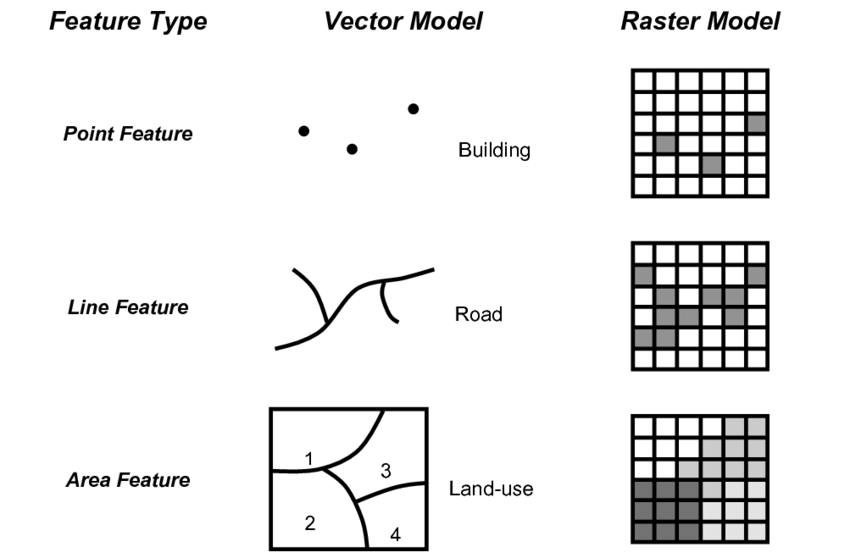
\includegraphics{images/data-models.png}

\hypertarget{spatial-thinking-in-epidemiology}{%
\section{Spatial Thinking in Epidemiology}\label{spatial-thinking-in-epidemiology}}

When first learning epidemiology, it can be difficult to distinguish between the concepts, theories, and purpose of epidemiology versus the skills, tools, and methods that we use to implement epidemiology. But these distinctions are foundational to our collective professional identity, and to the way we go about doing our work. For instance do you think of epidemiologists as data analysts, scientists, data scientists, technicians or something else? These questions are bigger than we can address in this class, but their importance becomes especially apparent when learning an area such as \emph{spatial epidemiology}. This is because there is a tendency for discourse in spatial epidemiology to focus primarily on the \emph{data} and the \emph{methods} without understanding how each of those relate to the \emph{scientific questions} and \emph{health of population} for which we are ultimately responsible. Distinguishing these threads is an overarching goal of this course, even as we learn the data science and spatial analytic tools.

One quite simplistic but important example of how our questions and methods are inter-related is apparent when we think of \textbf{data}. Data is central to quantitative analysis, including epidemiologic analysis. So how is \emph{data} different in \emph{spatial} epidemiology? The first thing that might come to mind is that we have explicitly geographic or spatial measures contained within our data. That the content of the spatial data is distinct: the addition of geographic or spatial location may illuminate otherwise \emph{aspatial} attributes. But even more fundamental than the content is thinking about the \emph{unit of analysis}.

It is likely that many other examples in your epidemiology coursework the explicit (or sometimes implicit) unit of analysis has been the individual person. Spatial epidemiology can definitely align with individual-level analysis. But as we'll see, common units we observe and measure in spatial epidemiology -- and therefore the units that compose much of our \textbf{data} -- are not individuals but instead are geographic units (e.g.~census tract, county, state, etc) and by extension the \emph{collection} or \emph{aggregation} of all the individuals therein. This distinction in unit of analysis has important implications for other epidemiologic concerns including precision, bias, and ultimately for inference (e.g.~the meaning we can make from our analysis), as we'll discuss throughout the semester.

One concrete implication of the above discussion is that you should always be able to answer a basic question about any dataset you wish to analyze: ``\emph{what does one row of data represent?}'' A row of data is one way to think of the \emph{unit of analysis}, and often (but not always) in spatial epidemiology a row of data is a summary of the population contained by a geographic unit. Said another way it is an \emph{ecologic summary} of the population. As stated above, this is only the most simplistic example of how and why it is important to not only learn the spatial statistics and methods, but to also maintain the perspective of epidemiology as a population health science. To advance public health we need good methods but we also need critical understanding of the populations we support, the data we analyze, and the conclusions we can reliably draw from our work.

As we move through the semester, I encourage you to dig deep into how methods work, but also to step back and ask questions like \emph{``Why would I choose this method?''} or \emph{``What question in epidemiology is this useful for?''}

\hypertarget{spatial-analysis-in-epidemiology}{%
\section{Spatial Analysis in Epidemiology}\label{spatial-analysis-in-epidemiology}}

\hypertarget{spatial-data-storage-foramts}{%
\subsection{Spatial data storage foramts}\label{spatial-data-storage-foramts}}

If you have worked with spatial or GIS data using ESRI's ArcMap, you will be familiar with what are called \emph{shapefiles}. This is one very common format for storing geographic data on computers. ESRI shapefiles are not actually a single file, but are anywhere from four to eight different files all with the same file name but different extensions (e.g.~\emph{.shp}, \emph{.prj}, \emph{.shx}, etc). Each different file (corresponding to an extension) contains a different portion of the data ranging from the geometry data, the attribute data, the projection data, an index connecting it all together, etc.

What you may not know is that shapefiles are not the only (and in my opinion \textbf{definitely not the best}) way to store geographic data. In this class I recommend storing data in a format called \emph{geopackages} indicated by the \passthrough{\lstinline!.gpkg!} extension. Geopackages are an open source format that were developed to be functional on mobile devices. They are useful when we are storing individual files in an efficient and compact way. To be clear, there are many other formats and I make no claim that \emph{geopackages} are the ultimate format; they just happen to meet the needs for this course, and for much of the work of spatial epidemiologists. It is worth noting that many GIS programs including ArcMap and QGIS can both read and write the geopackage format; so there is no constraint or limitation in terms of software when data are stored in \passthrough{\lstinline!.gpkg!} format.

\hypertarget{representing-spatial-data-in-r}{%
\subsection{\texorpdfstring{Representing spatial data in \texttt{R}}{Representing spatial data in R}}\label{representing-spatial-data-in-r}}

The work in this course assumes that you are a \emph{basic \passthrough{\lstinline!R!} user}; you do not need to be expert, but I assume that you understand data objects (e.g.~\passthrough{\lstinline!data.frame!}, \passthrough{\lstinline!list!}, \passthrough{\lstinline!vector!}), and basic operations including subsetting by index (e.g.~using square brackets to extract or modify information: \passthrough{\lstinline![]!}), base-R plotting, and simple modeling. If you \textbf{are not familiar with \passthrough{\lstinline!R!}}, you will need to do some quick self-directed learning. The instructor and TA's can point you to resources.

Just as our conceptualization of, or thinking about \emph{data} in spatial epidemiology requires some reflection, the actual storage and representation of that data with a computer tool such as \passthrough{\lstinline!R!} also requires some attention. Specifically spatial data in \passthrough{\lstinline!R!} is not exactly like the conventional \emph{aspatial} epidemiologic data which may exist in \passthrough{\lstinline!R!} as a rectangular \passthrough{\lstinline!data.frame!} for example, but it is also need not be as complex as spatial data in software platforms like ESRI's ArcMap.

First, it may be obvious, but spatial data is more complex than simple rectangular attribute data (e.g.~data tables where a row is an observation and a column is a variable). To be \emph{spatial}, a dataset must have a representation of geography, spatial location, or spatial relatedness, and that is most commonly done with either a \emph{vector} or \emph{raster} data model (see description above in vocabulary). Those spatial or geographic representations must be stored on your computer and/or held in memory, hopefully with a means for relating or associating the individual locations with their corresponding attributes. For example we want to know the attribute (e.g.~the count of deaths for a given place), and the location of that place, and ideally we want the two connected together.

Over the past 10+ years, \passthrough{\lstinline!R!} has increasingly been used to analyze and visualize spatial data. Early on, investigators tackling the complexities of spatial data analysis in \passthrough{\lstinline!R!} developed a number of ad hoc, one-off approaches to these data. This worked in the short term for specific applications, but it created new problems as users needed to generalize a method to a new situation, or chain together steps. In those settings it was not uncommon to convert a dataset to multiple different formats to accomplish all tasks; this resulted in convoluted and error-prone coding, and lack of transparency in analysis.

An eventual response to this early tumult was a thoughtful and systematic approach to defining a \emph{class of data} that tackled the unique challenges of spatial data in \passthrough{\lstinline!R!}. Roger Bivand, Edzer Pebesma and others developed the \passthrough{\lstinline!sp!} package which defined spatial data classes, and provided functional tools to interact with them. The \passthrough{\lstinline!sp!} package defined specific data classes to hold points, lines, and polygons, as well as raster/grid data; each of these data classes can contain geometry only (these have names like \passthrough{\lstinline!SpatialPoints!} or \passthrough{\lstinline!SpatialPolygons!}) or could contain geometry plus related data attributes (these have names like \passthrough{\lstinline!SPatialPointsDataFrame!} or \passthrough{\lstinline!SpatialPolygonsDataFrame!}). Each spatial object can contain all the information spatial data might include: the spatial extent (min/max x, y values), the coordinate system or spatial projection, the geometry information, the attribute information, etc.

Because of the flexibility and power of the \passthrough{\lstinline!sp*!} class of objects, they became a standard up until the last few years. Interestingly, it was perhaps the sophistication of the \passthrough{\lstinline!sp*!} class that began to undermine it. \passthrough{\lstinline!sp*!} class data was well-designed from a programming point of view, but was still a little cumbersome (and frankly confusing) for more applied analysts and new users. Analysis in \emph{spatial epidemiology} is not primarily about computer programming, but about producing transparent and reliable data pipelines to conduct valid, reliable, and reproducible analysis. Thus epidemiologists, and other data scientists, desired spatial tools that could be incorporated into the growing toolbox of data science tools in \passthrough{\lstinline!R!}.

These calls for a more user-friendly and intuitive approach to spatial data led the same team (e.g.~Bivand, Pebesma, others) to develop the \emph{Simple Features} set of spatial data classes for \passthrough{\lstinline!R!}. Loaded with the \passthrough{\lstinline!sf!} package, this data format has quickly become the standard for handling spatial data in \passthrough{\lstinline!R!}. The power of the \passthrough{\lstinline!sf!} class, as discussed below, is that it makes \emph{spatial data} behave like \emph{rectangular data} and thus makes it amenable to manipulation using any tool that works on \passthrough{\lstinline!data.frame!} or \passthrough{\lstinline!tibble!} objects. Recognizing that many users and functions prefer the older \passthrough{\lstinline!sp*!} objects, the \passthrough{\lstinline!sf!} package includes a number of utility functions for easily converting back and forth.

\textbf{In this class we will use \passthrough{\lstinline!sf*!} class objects as the preferred data class, but because some of the tools we'll learn require \passthrough{\lstinline!sp*!} we will occasionally go back and forth.}

\passthrough{\lstinline!sf*!} data classes are designed to hold all the essential spatial information (projection, extent, geometry), but do so with an easy to evaluate \passthrough{\lstinline!data.frame!} format that integrates the attribute information and the geometry information together. The result is more intuitive sorting, selecting, aggregating, and visualizing.

\hypertarget{benefits-of-sf-data-classes}{%
\subsection{\texorpdfstring{Benefits of \texttt{sf} data classes}{Benefits of sf data classes}}\label{benefits-of-sf-data-classes}}

As Robin Lovelace writes in his online eBook, \href{https://geocompr.robinlovelace.net/}{Gecomputation in R}, \passthrough{\lstinline!sf!} data classes offer an approach to spatial data that is compatible with QGIS and PostGIS, important non-ESRI open source GIS platforms, and \passthrough{\lstinline!sf!} functionality compared to \passthrough{\lstinline!sp!} provides:

\begin{enumerate}
\def\labelenumi{\arabic{enumi}.}
\tightlist
\item
  Fast reading and writing of data
\item
  Enhanced plotting performance
\item
  \passthrough{\lstinline!sf!} objects can be treated as data frames in most operations
\item
  \passthrough{\lstinline!sf!} functions can be combined using \passthrough{\lstinline!\%>\%!} pipe operator and works well with the \passthrough{\lstinline!tidyverse!} collection of \passthrough{\lstinline!R!} packages (\protect\hyperlink{dplyr}{see Tips for using \passthrough{\lstinline!dplyr!}} for examples)
\item
  \passthrough{\lstinline!sf!} function names are relatively consistent and intuitive (all begin with \passthrough{\lstinline!st\_!})
\end{enumerate}

\hypertarget{working-with-spatial-data-in-r}{%
\subsection{\texorpdfstring{Working with spatial data in \texttt{R}}{Working with spatial data in R}}\label{working-with-spatial-data-in-r}}

Here and in lab, one example dataset we will use, called \passthrough{\lstinline!ga.mvc!} quantifies the counts and rates of death from motor vehicle crashes in each of Georgia's \(n=159\) counties. The dataset is \emph{vector} in that it represents counties as polygons with associated attributes (e.g.~the mortality information, county names, etc).

\hypertarget{importing-spatial-data-into-r}{%
\subsubsection{\texorpdfstring{Importing spatial data into \texttt{R}}{Importing spatial data into R}}\label{importing-spatial-data-into-r}}

It is important to distinguish between two kinds of data formats. There is a way that data is \emph{stored on a computer hard drive}, and then there is a way that data is organized and managed \emph{inside a program} like \passthrough{\lstinline!R!}. The \emph{shapefiles} (\passthrough{\lstinline!.shp!}) popularized by ESRI/ArcMap is an example of a format for storing spatial data on a hard drive. In contrast, the discussion above about the \passthrough{\lstinline!sf*!} and \passthrough{\lstinline!sp*!} data classes refer to how data is organized \emph{inside \passthrough{\lstinline!R!}}. Luckily, regardless of how data is \emph{stored} on your computer, it is possible to import almost any format into \passthrough{\lstinline!R!}, and once inside \passthrough{\lstinline!R!} it is possible to make it into either the \passthrough{\lstinline!sp*!} or \passthrough{\lstinline!sf*!} data class. That means if you receive data as a \passthrough{\lstinline!.shp!} shapefile, as a \passthrough{\lstinline!.gpkg!} geopackage, or as a \passthrough{\lstinline!.tif!} raster file, each can be easily imported.

All \passthrough{\lstinline!sf!} functions that act on spatial objects begin with the prefix \passthrough{\lstinline!st\_!}. Therefore to import (read) data we will use \passthrough{\lstinline!st\_read()!}. This function determines \textbf{how} to import the data based on the extension of the file name you specify. Look at the help documentation for \passthrough{\lstinline!st\_read()!}. Notice that the first argument \passthrough{\lstinline!dsn=!}, might be a complete file name (e.g.~\passthrough{\lstinline!myData.shp!}), or it might be a folder name (e.g.~\passthrough{\lstinline!mygeodatabase.gdb!}). So if you had a the motor vehicle crash data saved as both a shapefile (\passthrough{\lstinline!mvc.shp!}, which is actually six different files on your computer), and as a geopackage (\passthrough{\lstinline!mvc.gpkg!}) you can read them in like this:

\begin{lstlisting}[language=R]
# this is the shapefile
mvc.a <- st_read('GA_MVC/ga_mvc.shp')

# this is the geopackage
mvc.b <- st_read('GA_MVC/ga_mvc.gpkg')
\end{lstlisting}

We can take a look at the defined data class of the imported objects within \passthrough{\lstinline!R!}:

\begin{lstlisting}[language=R]
class(mvc.a)
\end{lstlisting}

\begin{lstlisting}
## [1] "sf"         "data.frame"
\end{lstlisting}

\begin{lstlisting}[language=R]
class(mvc.b)
\end{lstlisting}

\begin{lstlisting}
## [1] "sf"         "data.frame"
\end{lstlisting}

First, note that when we use the \passthrough{\lstinline!st\_read()!} function, the data class (e.g.~the way the data are defined and organized \emph{within \passthrough{\lstinline!R!}}) is the same for both \passthrough{\lstinline!mvc.a!} (which started as a \passthrough{\lstinline!.shp!} file) and \passthrough{\lstinline!mvc.b!} (which started as a \passthrough{\lstinline!.gpkg!} file). That is because \passthrough{\lstinline!st\_read()!} automatically classifies spatial data using \passthrough{\lstinline!sf!} classes when it imports.

You will also notice that when we examined the \passthrough{\lstinline!class()!} of each object, they are classified as \textbf{both} \passthrough{\lstinline!sf!} \textbf{and} \passthrough{\lstinline!data.frame!} class. That is incredibly important, and it speaks to an elegant simplicity of the \passthrough{\lstinline!sf*!} data classes! That it is classified as \passthrough{\lstinline!sf!} is perhaps obvious; but the fact that each object is \emph{also classified} as \passthrough{\lstinline!data.frame!} means that we can treat the object for the purposes of data management, manipulation and analysis as a relatively simple-seeming object: a rectangular \passthrough{\lstinline!data.frame!}. How does that work? We will explore this more in lab but essentially each dataset has rows (observations) and columns (variables). We can see the variable/column names like this:

\begin{lstlisting}[language=R]
names(mvc.a)
\end{lstlisting}

\begin{lstlisting}
## [1] "GEOID"      "NAME"       "MVCRATE_17" "geometry"
\end{lstlisting}

\begin{lstlisting}[language=R]
names(mvc.b)
\end{lstlisting}

\begin{lstlisting}
## [1] "GEOID"      "NAME"       "MVCRATE_17" "geom"
\end{lstlisting}

We can see that each dataset has the same \emph{attribute} variables (e.g.~\passthrough{\lstinline!GEOID!}, \passthrough{\lstinline!NAME!}, \passthrough{\lstinline!MVCRATE\_17!}), and then a final column called \passthrough{\lstinline!geometry!} in one and called \passthrough{\lstinline!geom!} in another. These geometry columns are unique in that they don't hold a single value like the other columns; each \emph{`cell'} in those columns actually contains an embedded list of \(x,y\) coordinates defining the vertices of the polygons for each of Georgia's counties.

Combining these two observations, we now know that we can work with a wide range of spatial data formats, and that once imported we can conceive of (and manipulate!) these data almost as if they were simple rectangular datasets. This has implications for subsetting, recoding, merging, and aggregating data as we'll learn in the coming weeks.

\hypertarget{exporting-spatial-data-from-r}{%
\subsubsection{\texorpdfstring{Exporting spatial data from \texttt{R}}{Exporting spatial data from R}}\label{exporting-spatial-data-from-r}}

While importing is often the primary challenge with spatial data and \passthrough{\lstinline!R!}, it is not uncommon that you might modify or alter a spatial dataset and wish to save it for future use, or to write it out to disk to share with a colleague. Luckily the \passthrough{\lstinline!sf!} package has the same functionality to write an \passthrough{\lstinline!sf!} spatial object to disk in a wide variety of formats including \emph{shapefiles} (\passthrough{\lstinline!.shp!}) and \emph{geopackages} (\passthrough{\lstinline!.gpkg!}). Again, \passthrough{\lstinline!R!} uses the extension you specify in the filename to determine the target format.

\begin{lstlisting}[language=R]
# Write the file mvc to disk as a shapefile format
st_write(mvc, 'GA_MVC/ga_mvc_v2.shp')

# Write the file mvc to disk as a geopackage format
st_write(mvc, 'GA_MVC/ga_mvc_v2.gpkg')
\end{lstlisting}

\hypertarget{basic-visual-inspectionplots}{%
\subsection{Basic visual inspection/plots}\label{basic-visual-inspectionplots}}

The base-R \passthrough{\lstinline!plot()!} function is extended by the \passthrough{\lstinline!sf!} package. That means that if you call \passthrough{\lstinline!plot()!} on a spatial object \textbf{without having loaded} \passthrough{\lstinline!sf!}, the results will be different than if \passthrough{\lstinline!plot()!} called \textbf{after loading} \passthrough{\lstinline!sf!}.

When you \passthrough{\lstinline!plot()!} with \passthrough{\lstinline!sf!}, by default it will try to make a map \textbf{for every variable in the data frame}! Try it once. If this is not what you want, you can force it to only plot \emph{some} variables by providing a vector of variable names.

\begin{lstlisting}[language=R]
plot(mvc) # this plots a panel for every column - or actually the first 10 columns
\end{lstlisting}

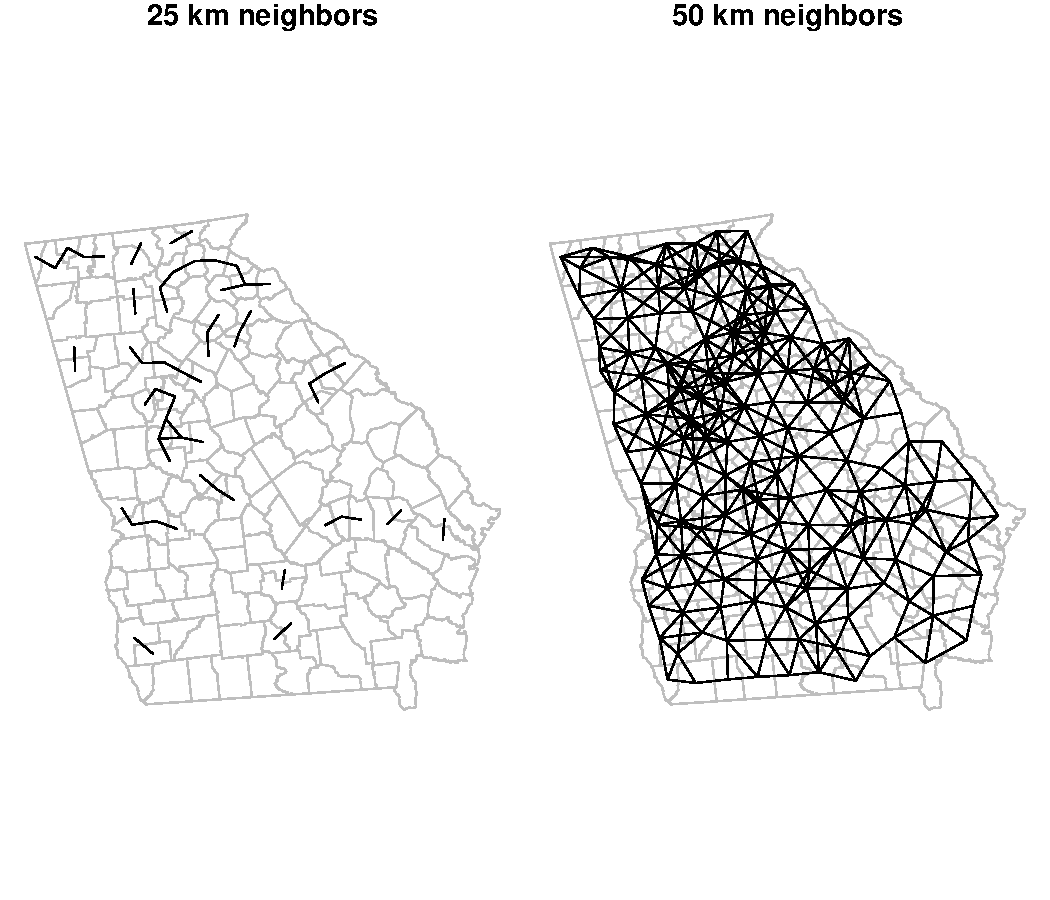
\includegraphics{EPI563-SpatialEPI_files/figure-latex/unnamed-chunk-16-1.pdf}

\begin{lstlisting}[language=R]
plot(mvc['MVCRATE_05']) # this plots only a single variable, the MVC mortality rate for 2005
\end{lstlisting}

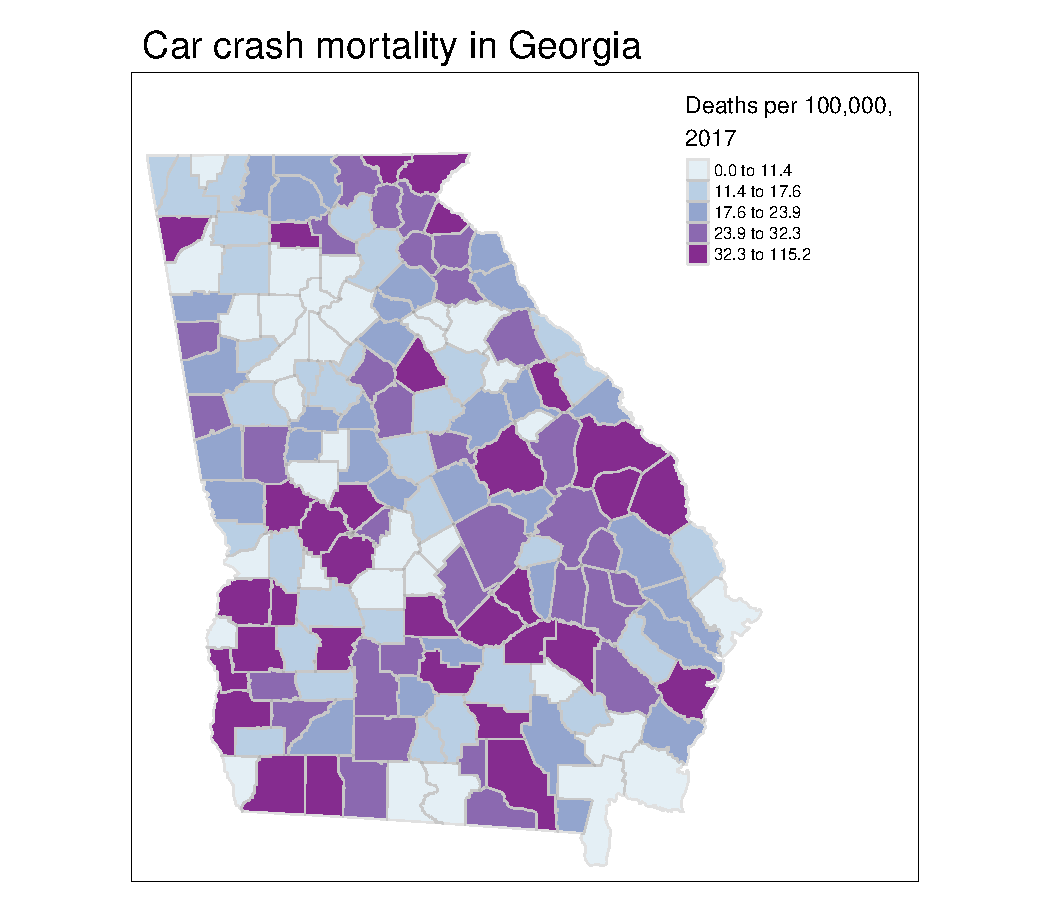
\includegraphics{EPI563-SpatialEPI_files/figure-latex/unnamed-chunk-17-1.pdf}

\begin{lstlisting}[language=R]
plot(mvc[c('MVCRATE_05', 'MVCRATE_17')]) # this plots two variables: MVC rate in 2005 & 2017
\end{lstlisting}

\includegraphics{EPI563-SpatialEPI_files/figure-latex/unnamed-chunk-17-2.pdf}

You might only want to see the geometry of the spatial object (e.g.~not attributes) if you are checking its extent, the scale, or otherwise confirming something about the spatial aspects of the object. Here are two approaches to quickly plot the geometry:

\begin{lstlisting}[language=R]
plot(st_geometry(mvc)) # st_geometry() returns the geom information to plot
\end{lstlisting}

\begin{lstlisting}[language=R]
plot(mvc$geom)  # this is an alternative approach...directly plot the 'geom' column
\end{lstlisting}

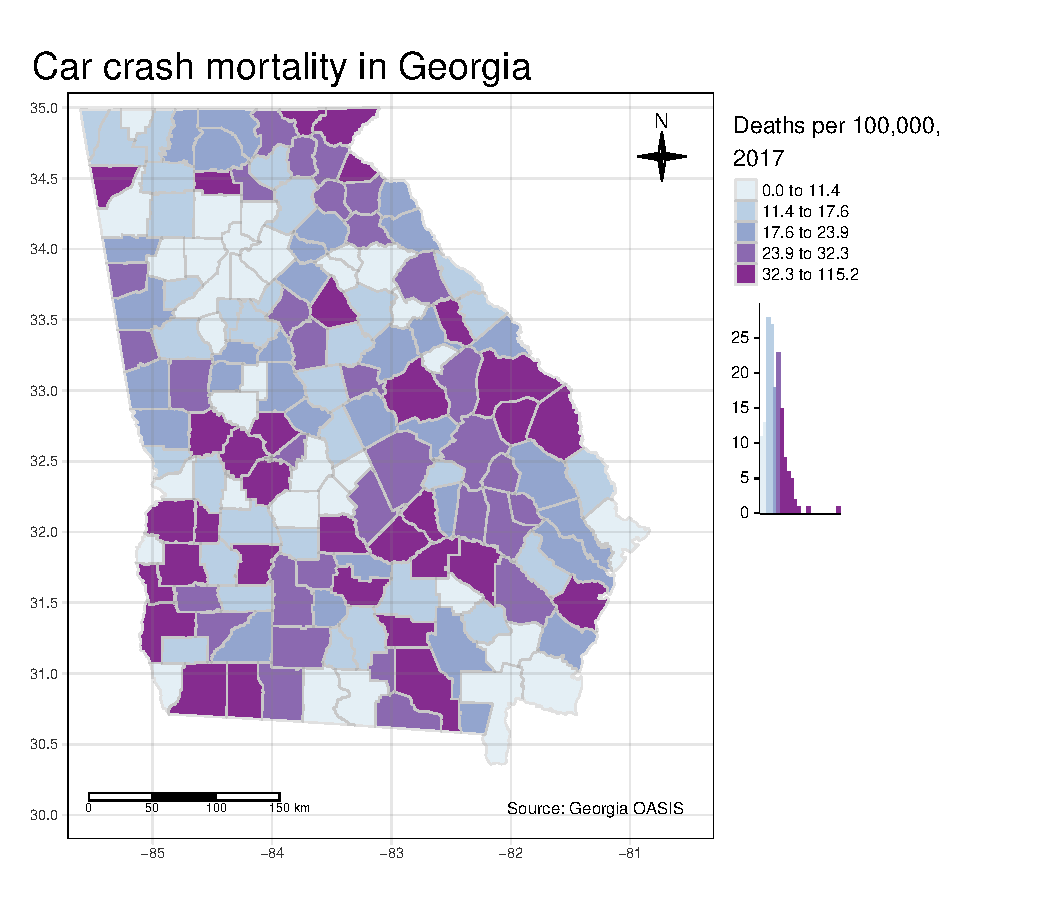
\includegraphics{EPI563-SpatialEPI_files/figure-latex/unnamed-chunk-19-1.pdf}

\hypertarget{working-with-crs-and-projection}{%
\subsection{Working with CRS and projection}\label{working-with-crs-and-projection}}

If CRS (coordinate reference system) and projection information was contained in the original file you imported, it will be maintained. \textbf{If there is NO CRS information imported it is critical that you find out the CRS information from the data source!} The most unambiguous way to describe a projection is by using the \textbf{EPSG} code, which stands for \emph{European Petroleum Survey Group}. This consortium has standardized hundreds of projection definitions in a manner adopted by several \passthrough{\lstinline!R!} packages including \passthrough{\lstinline!rgdal!} and \passthrough{\lstinline!sf!}.

This course is not a GIS course, and learning about the theory and application of coordinate reference systems and projections is not our primary purpose. However some basic knowledge \emph{is necessary} for successfully working with spatial epidemiologic data. Here are several resources you should peruse to learn more about CRS, projections, and EPSG codes:

\begin{itemize}
\tightlist
\item
  \href{https://www.nceas.ucsb.edu/sites/default/files/2020-04/OverviewCoordinateReferenceSystems.pdf}{A useful overview/review of coordinate reference systems in \passthrough{\lstinline!R!}}
\item
  \href{https://geocompr.robinlovelace.net/reproj-geo-data.html}{Robin Lovelace's Geocompuation in R on projections with \passthrough{\lstinline!sf!}}
\item
  \href{https://epsg.io/}{EPSG website:} This link is to a searchable database of valid ESPG codes
\item
  \href{https://guides.library.duke.edu/r-geospatial/CRS}{Here are some useful EPSG codes}
\end{itemize}

\begin{figure}
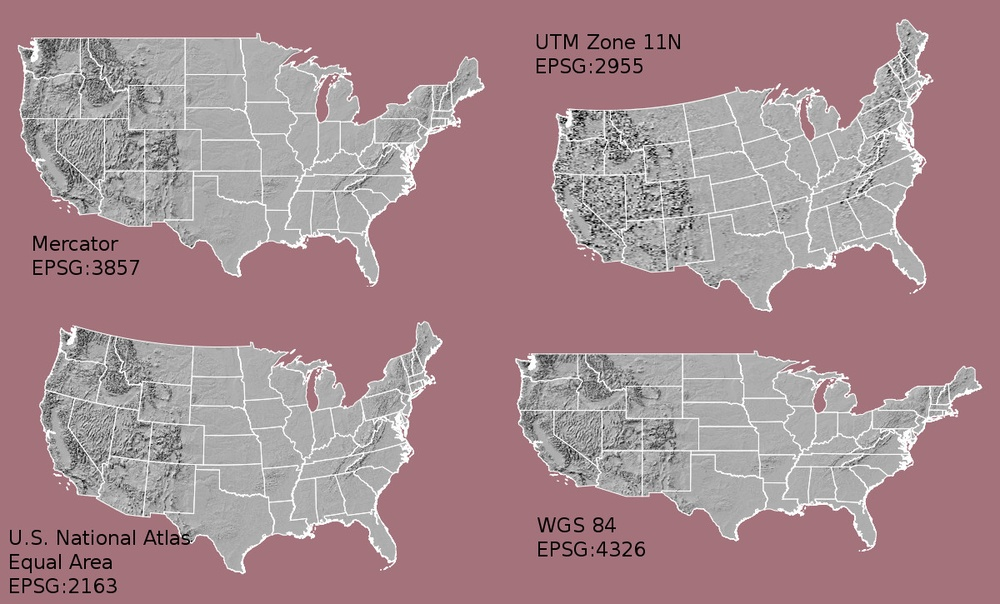
\includegraphics[width=0.5\linewidth]{images/compare-crs} \caption{Comparing CRS}\label{fig:unnamed-chunk-20}
\end{figure}

The choice of CRS and/or projection has a substantial impact on how the produced map looks, as is evident in the figure above (\href{https://datacarpentry.org/organization-geospatial/03-crs/}{source of image}).

We already saw the CRS/projection information of the \passthrough{\lstinline!mvc!} object when we used the \passthrough{\lstinline!head()!} function above; it was at the top and read \passthrough{\lstinline!WGS 84!}. Recall there are two main types of CRS: purely \textbf{geographic} which is to say coordinate locations are represented as \emph{latitude} and \emph{longitude} degrees; and \textbf{projected} which means the coordinate values have been transformed for representation of the spherical geoid onto a planar (Euclidean) coordinate system. \passthrough{\lstinline!WGS 84!} is a ubiquitous geographic coordinate system common to boundary files retrieved from the U.S. Census bureau.

An important question when you work with a spatial dataset is to understand whether it is primarily a geographic or projected CRS, and if so which one.

\begin{lstlisting}[language=R]
st_is_longlat(mvc)
\end{lstlisting}

\begin{lstlisting}
## [1] TRUE
\end{lstlisting}

This quick logical test returns \passthrough{\lstinline!TRUE!} or \passthrough{\lstinline!FALSE!} to answer the question \emph{``Is the \passthrough{\lstinline!sf!} object simply a longitude/latitude geographic CRS?''}. The answer in this case is \passthrough{\lstinline!TRUE!} because \passthrough{\lstinline!WGS 84!} is a geographic (longlat) coordinate system. But what if it were \passthrough{\lstinline!FALSE!} or we wanted to know more about the CRS/projection?

\begin{lstlisting}[language=R]
st_crs(mvc)
\end{lstlisting}

\begin{lstlisting}
## Coordinate Reference System:
##   User input: WGS 84 
##   wkt:
## GEOGCRS["WGS 84",
##     DATUM["World Geodetic System 1984",
##         ELLIPSOID["WGS 84",6378137,298.257223563,
##             LENGTHUNIT["metre",1]]],
##     PRIMEM["Greenwich",0,
##         ANGLEUNIT["degree",0.0174532925199433]],
##     CS[ellipsoidal,2],
##         AXIS["geodetic latitude (Lat)",north,
##             ORDER[1],
##             ANGLEUNIT["degree",0.0174532925199433]],
##         AXIS["geodetic longitude (Lon)",east,
##             ORDER[2],
##             ANGLEUNIT["degree",0.0174532925199433]],
##     USAGE[
##         SCOPE["unknown"],
##         AREA["World"],
##         BBOX[-90,-180,90,180]],
##     ID["EPSG",4326]]
\end{lstlisting}

This somewhat complicated looking output is a summary of the CRS stored with the spatial object. There are two things to note about this output:

\begin{itemize}
\tightlist
\item
  At the top, the \emph{User input} is \passthrough{\lstinline!WGS 84!}
\item
  At the bottom of the section labeled \passthrough{\lstinline!GEOGCRS!} it says \passthrough{\lstinline!ID["EPSG",4326"]!}
\end{itemize}

While there are literally hundreds of distinct EPSG codes describing different geographic and projected coordinate systems, for this semester there are three worth remembering:

\begin{itemize}
\tightlist
\item
  \textbf{EPSG: 4326} is a common geographic (unprojected or long-lat) CRS
\item
  \textbf{EPSG: 3857} is also called \emph{WGS 84/Web Mercator}, and is the dominant CRS used by Google Maps
\item
  \textbf{EPSG: 5070} is the code for a projected CRS called \emph{Albers Equal Area} which has the benefit of representing the visual area of maps in an equal manner.
\end{itemize}

Once the CRS/projection is clearly defined, you may choose to transform or \emph{project} the data to a different system. The \passthrough{\lstinline!sf!} package has another handy function called \passthrough{\lstinline!st\_transform()!} that takes in a spatial object (dtaaset) with one CRS and outputs that object \emph{transformed} to a new CRS.

\begin{lstlisting}[language=R]
# This uses the Albers equal area USA, 
mvc.aea <- st_transform(mvc, 5070)

# This uses the Web Mercator CRS (EPSG 3857) which is just barely different from EPSG 4326
mvc.wm <- st_transform(mvc, 3857)

# Now let's look at them side-by-side
plot(st_geometry(mvc), main = 'EPSG 4326')
plot(st_geometry(mvc.wm), main = 'Web Mercator (3857)')
plot(st_geometry(mvc.aea), main = 'Albers Equal Area (5070)')
\end{lstlisting}

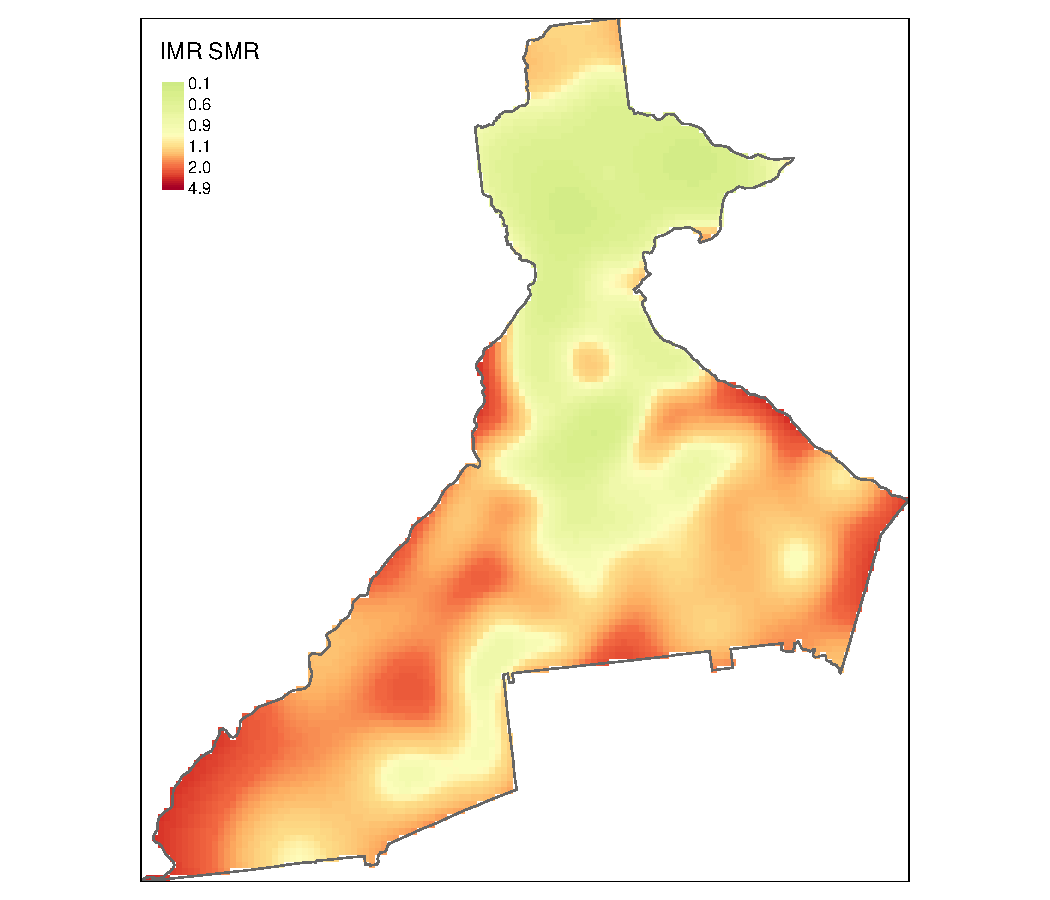
\includegraphics{EPI563-SpatialEPI_files/figure-latex/unnamed-chunk-24-1.pdf}

Do you see the difference between the three? Because EPSG 4326 and 3857 are both unprojected (e.g.~they are long/lat), they appear quite similar but are not identical. Albers Equal Area, on the other hand, is more distinct. In general we will prefer to use \emph{`projected'} rather than \emph{`unprojected'} (long/lat only) data for both visualization and analysis. That means that whenever you bring in a new dataset you will need to check the CRS and project or transform as desired.

\begin{rmdcaution}
\textbf{Important:} It is important to distinguish between defining the current projection of data and the act of \emph{projecting} or \emph{transforming} data from one known system to a new CRS/projection. \textbf{We cannot transform data until we correctly define its current or original CRS/projection status.} The above function tells us what the current status is. In some cases data do not have associated CRS information and this might be completely blank (for instance if you read in numerical \(x,y\) points from a geocoding or GPS process). In those cases you can \textbf{set} the underlying CRS using \passthrough{\lstinline!st\_set\_crs()!} to define it, but this assumes you \textbf{know} what it is. There are two arguments to this function: the first is \passthrough{\lstinline!x = objectName!}, and the second is \passthrough{\lstinline!value = xxx!} where \emph{`xxx'} is a valid EPSG code.
\end{rmdcaution}

\hypertarget{cartography-for-epidemiology-i}{%
\chapter{Cartography for Epidemiology I}\label{cartography-for-epidemiology-i}}

\hypertarget{getting-ready}{%
\section{Getting Ready}\label{getting-ready}}

\hypertarget{learning-objectives-w2}{%
\subsection{Learning objectives, w2}\label{learning-objectives-w2}}

 
  \providecommand{\huxb}[2]{\arrayrulecolor[RGB]{#1}\global\arrayrulewidth=#2pt}
  \providecommand{\huxvb}[2]{\color[RGB]{#1}\vrule width #2pt}
  \providecommand{\huxtpad}[1]{\rule{0pt}{#1}}
  \providecommand{\huxbpad}[1]{\rule[-#1]{0pt}{#1}}

\begin{table}[ht]
\begin{centerbox}
\begin{threeparttable}
\captionsetup{justification=centering,singlelinecheck=off}
\caption{\label{tab:learning-ob} Learning objectives by weekly module}
 \setlength{\tabcolsep}{0pt}
\begin{tabularx}{1\textwidth}{p{1\textwidth}}


\hhline{>{\huxb{255, 255, 255}{1}}-}
\arrayrulecolor{black}

\multicolumn{1}{!{\huxvb{255, 255, 255}{1}}p{1\textwidth}!{\huxvb{255, 255, 255}{1}}}{\cellcolor[RGB]{208, 211, 212}\hspace{6pt}\parbox[b]{1\textwidth-6pt-6pt}{\huxtpad{2pt + 1em}\raggedright \textbf{After this module you should be able to…}\huxbpad{2pt}}} \tabularnewline[-0.5pt]


\hhline{>{\huxb{255, 255, 255}{1}}-}
\arrayrulecolor{black}

\multicolumn{1}{!{\huxvb{255, 255, 255}{1}}p{1\textwidth}!{\huxvb{255, 255, 255}{1}}}{\cellcolor[RGB]{250, 229, 211}\hspace{6pt}\parbox[b]{1\textwidth-6pt-6pt}{\huxtpad{2pt + 1em}\raggedright Design a cartographic representation of epidemiologic data that is consistent with best practices in public health data visualization.\huxbpad{2pt}}} \tabularnewline[-0.5pt]


\hhline{>{\huxb{255, 255, 255}{1}}-}
\arrayrulecolor{black}

\multicolumn{1}{!{\huxvb{255, 255, 255}{1}}p{1\textwidth}!{\huxvb{255, 255, 255}{1}}}{\cellcolor[RGB]{245, 203, 167}\hspace{6pt}\parbox[b]{1\textwidth-6pt-6pt}{\huxtpad{2pt + 1em}\raggedright Apply data processing functions to accomplish foundational data management and preparation for spatial epidemiology (e.g. summarize, aggregate, combine, recode, etc)\huxbpad{2pt}}} \tabularnewline[-0.5pt]


\hhline{>{\huxb{255, 255, 255}{1}}-}
\arrayrulecolor{black}
\end{tabularx}
\end{threeparttable}\par\end{centerbox}

\end{table}
 

\hypertarget{additional-resources-w2}{%
\subsection{Additional Resources, w2}\label{additional-resources-w2}}

\begin{itemize}
\tightlist
\item
  \href{https://www.cdc.gov/dhdsp/maps/gisx/resources/tips-creating-ph-maps.html}{CDC Guidance for Cartography of Public Health Data (complements required reading)}
\item
  \href{https://www.citylab.com/design/2015/06/when-maps-lie/396761/}{When Maps Lie}
\item
  \href{http://colorbrewer2.org/\#}{Color Brewer Website for color guidance in choropleth maps}
\end{itemize}

\hypertarget{important-vocabulary-w2}{%
\subsection{Important Vocabulary, w2}\label{important-vocabulary-w2}}

 
  \providecommand{\huxb}[2]{\arrayrulecolor[RGB]{#1}\global\arrayrulewidth=#2pt}
  \providecommand{\huxvb}[2]{\color[RGB]{#1}\vrule width #2pt}
  \providecommand{\huxtpad}[1]{\rule{0pt}{#1}}
  \providecommand{\huxbpad}[1]{\rule[-#1]{0pt}{#1}}

\begin{table}[ht]
\begin{centerbox}
\begin{threeparttable}
\captionsetup{justification=centering,singlelinecheck=off}
\caption{\label{tab:unnamed-chunk-28} Vocabulary for Week 2}
 \setlength{\tabcolsep}{0pt}
\begin{tabularx}{0.9\textwidth}{p{0.45\textwidth} p{0.45\textwidth}}


\hhline{>{\huxb{255, 255, 255}{1}}->{\huxb{255, 255, 255}{1}}-}
\arrayrulecolor{black}

\multicolumn{1}{!{\huxvb{255, 255, 255}{1}}p{0.45\textwidth}!{\huxvb{255, 255, 255}{1}}}{\cellcolor[RGB]{84, 153, 199}\hspace{6pt}\parbox[b]{0.45\textwidth-6pt-2pt}{\huxtpad{2pt + 1em}\raggedright \textbf{\textcolor[RGB]{255, 255, 255}{Term}}\huxbpad{2pt}}} &
\multicolumn{1}{p{0.45\textwidth}!{\huxvb{255, 255, 255}{1}}}{\cellcolor[RGB]{84, 153, 199}\hspace{2pt}\parbox[b]{0.45\textwidth-2pt-6pt}{\huxtpad{2pt + 1em}\raggedright \textbf{\textcolor[RGB]{255, 255, 255}{Definition}}\huxbpad{2pt}}} \tabularnewline[-0.5pt]


\hhline{>{\huxb{255, 255, 255}{1}}->{\huxb{255, 255, 255}{1}}-}
\arrayrulecolor{black}

\multicolumn{1}{!{\huxvb{255, 255, 255}{1}}p{0.45\textwidth}!{\huxvb{255, 255, 255}{1}}}{\cellcolor[RGB]{212, 230, 241}\hspace{6pt}\parbox[b]{0.45\textwidth-6pt-2pt}{\huxtpad{2pt + 1em}\raggedright \textbf{Cartography}\huxbpad{2pt}}} &
\multicolumn{1}{p{0.45\textwidth}!{\huxvb{255, 255, 255}{1}}}{\cellcolor[RGB]{212, 230, 241}\hspace{2pt}\parbox[b]{0.45\textwidth-2pt-6pt}{\huxtpad{2pt + 1em}\raggedright The production of maps, including construction of projections, design, compilation, drafting, and reproduction\huxbpad{2pt}}} \tabularnewline[-0.5pt]


\hhline{>{\huxb{255, 255, 255}{1}}->{\huxb{255, 255, 255}{1}}-}
\arrayrulecolor{black}

\multicolumn{1}{!{\huxvb{255, 255, 255}{1}}p{0.45\textwidth}!{\huxvb{255, 255, 255}{1}}}{\cellcolor[RGB]{169, 204, 227}\hspace{6pt}\parbox[b]{0.45\textwidth-6pt-2pt}{\huxtpad{2pt + 1em}\raggedright \textbf{Choropleth map}\huxbpad{2pt}}} &
\multicolumn{1}{p{0.45\textwidth}!{\huxvb{255, 255, 255}{1}}}{\cellcolor[RGB]{169, 204, 227}\hspace{2pt}\parbox[b]{0.45\textwidth-2pt-6pt}{\huxtpad{2pt + 1em}\raggedright A type of thematic map in which areas are shaded or patterned in proportion to a statistical variable that represents an aggregate summary of a geographic characteristic within each area, such as population density, disease risk, or standardized mortality ratio\huxbpad{2pt}}} \tabularnewline[-0.5pt]


\hhline{>{\huxb{255, 255, 255}{1}}->{\huxb{255, 255, 255}{1}}-}
\arrayrulecolor{black}

\multicolumn{1}{!{\huxvb{255, 255, 255}{1}}p{0.45\textwidth}!{\huxvb{255, 255, 255}{1}}}{\cellcolor[RGB]{212, 230, 241}\hspace{6pt}\parbox[b]{0.45\textwidth-6pt-2pt}{\huxtpad{2pt + 1em}\raggedright \textbf{Color palette: diverging}\huxbpad{2pt}}} &
\multicolumn{1}{p{0.45\textwidth}!{\huxvb{255, 255, 255}{1}}}{\cellcolor[RGB]{212, 230, 241}\hspace{2pt}\parbox[b]{0.45\textwidth-2pt-6pt}{\huxtpad{2pt + 1em}\raggedright Diverging schemes allow the emphasis of a quantitative data display to be progressions outward from a critical midpoint of the data range. A typical diverging scheme pairs sequential schemes based on two different hues so that they diverge from a shared light color, for the critical midpoint, toward dark colors of different hues at each extreme\huxbpad{2pt}}} \tabularnewline[-0.5pt]


\hhline{>{\huxb{255, 255, 255}{1}}->{\huxb{255, 255, 255}{1}}-}
\arrayrulecolor{black}

\multicolumn{1}{!{\huxvb{255, 255, 255}{1}}p{0.45\textwidth}!{\huxvb{255, 255, 255}{1}}}{\cellcolor[RGB]{169, 204, 227}\hspace{6pt}\parbox[b]{0.45\textwidth-6pt-2pt}{\huxtpad{2pt + 1em}\raggedright \textbf{Color palette: qualitative}\huxbpad{2pt}}} &
\multicolumn{1}{p{0.45\textwidth}!{\huxvb{255, 255, 255}{1}}}{\cellcolor[RGB]{169, 204, 227}\hspace{2pt}\parbox[b]{0.45\textwidth-2pt-6pt}{\huxtpad{2pt + 1em}\raggedright Qualitative schemes use differences in hue to represent nominal differences, or differences in kind. The lightness of the hues used for qualitative categories should be similar but not equal. \huxbpad{2pt}}} \tabularnewline[-0.5pt]


\hhline{>{\huxb{255, 255, 255}{1}}->{\huxb{255, 255, 255}{1}}-}
\arrayrulecolor{black}

\multicolumn{1}{!{\huxvb{255, 255, 255}{1}}p{0.45\textwidth}!{\huxvb{255, 255, 255}{1}}}{\cellcolor[RGB]{212, 230, 241}\hspace{6pt}\parbox[b]{0.45\textwidth-6pt-2pt}{\huxtpad{2pt + 1em}\raggedright \textbf{Color palette: sequential}\huxbpad{2pt}}} &
\multicolumn{1}{p{0.45\textwidth}!{\huxvb{255, 255, 255}{1}}}{\cellcolor[RGB]{212, 230, 241}\hspace{2pt}\parbox[b]{0.45\textwidth-2pt-6pt}{\huxtpad{2pt + 1em}\raggedright Sequential data classes are logically arranged from high to low, and this stepped sequence of categories should be represented by sequential lightness steps. Low data values are usually represented by light colors and high values represented by dark colors. Transitions between hues may be used in a sequential scheme, but the light-to-dark progression should dominate the scheme.\huxbpad{2pt}}} \tabularnewline[-0.5pt]


\hhline{>{\huxb{255, 255, 255}{1}}->{\huxb{255, 255, 255}{1}}-}
\arrayrulecolor{black}

\multicolumn{1}{!{\huxvb{255, 255, 255}{1}}p{0.45\textwidth}!{\huxvb{255, 255, 255}{1}}}{\cellcolor[RGB]{169, 204, 227}\hspace{6pt}\parbox[b]{0.45\textwidth-6pt-2pt}{\huxtpad{2pt + 1em}\raggedright \textbf{Isopleth map}\huxbpad{2pt}}} &
\multicolumn{1}{p{0.45\textwidth}!{\huxvb{255, 255, 255}{1}}}{\cellcolor[RGB]{169, 204, 227}\hspace{2pt}\parbox[b]{0.45\textwidth-2pt-6pt}{\huxtpad{2pt + 1em}\raggedright A type of thematic map that uses contour lines or colors to indicate areas with similar regional aspects. It typically symbolizes the underlying statistic as varying continuously in space, in contrast to the discrete unit-specific variation of choropleth maps\huxbpad{2pt}}} \tabularnewline[-0.5pt]


\hhline{>{\huxb{255, 255, 255}{1}}->{\huxb{255, 255, 255}{1}}-}
\arrayrulecolor{black}

\multicolumn{1}{!{\huxvb{255, 255, 255}{1}}p{0.45\textwidth}!{\huxvb{255, 255, 255}{1}}}{\cellcolor[RGB]{212, 230, 241}\hspace{6pt}\parbox[b]{0.45\textwidth-6pt-2pt}{\huxtpad{2pt + 1em}\raggedright \textbf{Standardize Morbidity/Mortality Ratio (SMR)}\huxbpad{2pt}}} &
\multicolumn{1}{p{0.45\textwidth}!{\huxvb{255, 255, 255}{1}}}{\cellcolor[RGB]{212, 230, 241}\hspace{2pt}\parbox[b]{0.45\textwidth-2pt-6pt}{\huxtpad{2pt + 1em}\raggedright The ratio of observed to expected disease morbidity or mortality. Often the 'expected' is defined as the overall population (or study-specific) rate; in that case the SMR indicates the relative deviation of a specific unit from the global or overall rate\huxbpad{2pt}}} \tabularnewline[-0.5pt]


\hhline{>{\huxb{255, 255, 255}{1}}->{\huxb{255, 255, 255}{1}}-}
\arrayrulecolor{black}

\multicolumn{1}{!{\huxvb{255, 255, 255}{1}}p{0.45\textwidth}!{\huxvb{255, 255, 255}{1}}}{\cellcolor[RGB]{169, 204, 227}\hspace{6pt}\parbox[b]{0.45\textwidth-6pt-2pt}{\huxtpad{2pt + 1em}\raggedright \textbf{Visual hierarchy}\huxbpad{2pt}}} &
\multicolumn{1}{p{0.45\textwidth}!{\huxvb{255, 255, 255}{1}}}{\cellcolor[RGB]{169, 204, 227}\hspace{2pt}\parbox[b]{0.45\textwidth-2pt-6pt}{\huxtpad{2pt + 1em}\raggedright The apparent order of importance of phenomena perceived by the human eye.  In cartography, this principle is a fundamental part of map composition; since the goal of map composition is to clearly convey a desired purpose, the attention of readers should be focused on the map elements that are most relevant to the purpose.\huxbpad{2pt}}} \tabularnewline[-0.5pt]


\hhline{>{\huxb{255, 255, 255}{1}}->{\huxb{255, 255, 255}{1}}-}
\arrayrulecolor{black}
\end{tabularx}
\end{threeparttable}\par\end{centerbox}

\end{table}
 

\hypertarget{spatial-thinking-in-epidemiology-w2}{%
\section{Spatial Thinking in Epidemiology, w2}\label{spatial-thinking-in-epidemiology-w2}}

Making pretty maps is not the full extent of spatial epidemiology. However, \emph{epidemiologic cartography} can sometimes be the beginning and end of \emph{spatial epidemiology} for a given purpose. And even when an epidemiologic analysis goes well beyond mapping (perhaps to incorporate \emph{aspatial} analysis, or to incorporate more sophisticated \emph{spatial} analysis), the ability to produce a clear, concise, and interpretable map is an important skill.

As Robb, et al\footnote{Robb SW, Bauer SE, Vena JE. Integration of Different Epidemiological Perspectives and Applications to Spatial Epidemiology. Chapter 1 in Handbook of Spatial Epidemiology. 2016. CRC Press, Boca Raton, FL.} write:

\begin{quote}
Disease mapping can be used to provide \emph{visual cues} about disease etiology, particularly as it relates to environmental exposures\ldots.Mapping where things are allows visualization of a baseline pattern or spatial structure of disease, potential detection of disease clusters, and the initial investigation of an exposure-disease relationship.
\end{quote}

There are aspects of cartography and map design that are general to most thematic maps of quantitative data. But there are some issues that seem especially pertinent to us as epidemiologists or quantitative population health scientists. These include the decisions we make about color choice and the process of categorizing numerical data for visual representation in a map.

Why are these especially important for epidemiology? A primary purpose of a map is to visually represent \emph{something meaningful} about the \emph{spatial or geographic variation} in health or a health-relevant feature (e.g.~an exposure or resource). Communicating what is \emph{meaningful} and representing \emph{variation} that matters is not solely a technical GIS task; it requires epidemiologic insight. For instance our approach to representing ratio measures such as an \emph{odds ratio} or \emph{risk ratio} should be different from how we represent \emph{risk} or \emph{rate} data, because we understand that the scale and units are distinct in each case. Similarly, we understand that understanding variation or heterogeneity in a \emph{normal} or \emph{Gaussian} (bell-shaped curve) distribution is different from a uniform or a highly skewed distribution with a long right tail. This insight into how scales and values are differently interpretted epidemiologically muts be translated into sensible choices in mapping.

\hypertarget{color-choices}{%
\subsection{Color choices}\label{color-choices}}

For most thematic maps, color is the most flexible and important tools for communication. Color, hue, and contrast can accentuate map elements or themes and minimize others. The result is that you can completely change the story your map tells with seemingly small changes to how you use color. This means you should be clear and explicit about \emph{why you choose} a given color or sequence of colors, and beware of unintentionally misrepresenting your data by your color choices.

In producing choropleth maps, we often talk about collections of colors as \emph{color ramps} or \emph{color palettes}, because a single color by itself is not very interesting. A quick scan of either the \passthrough{\lstinline!tmaptools::palette\_explorer()!} utility, or \href{http://colorbrewer2.org/\#}{the Color Brewer website} will demonstrate that there are many colors to choose from, so is it just a matter of preference? Perhaps, but there are some guidelines to keep in mind.

\hypertarget{sequential-palettes}{%
\subsubsection{Sequential palettes}\label{sequential-palettes}}

All color palettes use the color hue, value, or saturation to represent or symbolize the values of the underlying statistical parameter of interest. When a parameter or statistic is naturally ordered, sequential and monotonic, then it makes sense to choose colors that range from light to dark. Conventionally \emph{lighter} or more neutral tones represent lower or smaller numbers and \emph{darker} colors and more intense tones represent higher or larger numbers. The dark colors jump out at the viewer more readily, so occasionally the inverse is used to emphasize small values, but this should be done with caution as it can be counterintuitive.

\begin{figure}
\centering
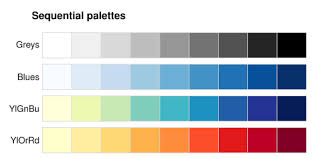
\includegraphics{images/palette-sequential.png}
\caption{\label{fig:unnamed-chunk-29}Sequential color palettes}
\end{figure}

\begin{rmdnote}
Sequential palettes are useful for epidemiologic parameters such as prevalence, risk, or rates, or continuous exposure values where the emphasis is on distinguishing higher values from lower values.
\end{rmdnote}

\hypertarget{diverging-palettes}{%
\subsubsection{Diverging palettes}\label{diverging-palettes}}

A less common choice, but one that is especially important for some epidemiologic parameters, is the diverging palette. In this pattern, the \emph{neutral color} is in the center of the sequence, with two different color hues become darker and more intense as they go out from the center.

\begin{figure}
\centering
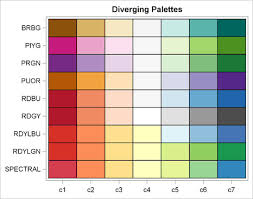
\includegraphics{images/palette-diverging.png}
\caption{\label{fig:unnamed-chunk-31}Diverging color palettes}
\end{figure}

You might choose this color sequence for one of two reasons:

\begin{enumerate}
\def\labelenumi{\arabic{enumi}.}
\tightlist
\item
  You wish to show how units vary around the overall mean or median, highlighting those that are \emph{larger than} versus \emph{smaller than} the overall mean/median. For instance diverging palettes might emphasize areas with particularly high burden of disease (and therefore in need of additional attention), as well as those with unexpectedly low burden of disease (and therefore worthy of understanding about protective factors).
\item
  You are mapping \emph{any epidemiologic parameter on the ratio scale} where there are values both above and below the null ratio of \(1.0\). For example if you map \emph{Standardized Mortality/Morbidity Ratios}, \emph{risk or odds ratios}, or \emph{prevalence ratios}, you potentially have diverging data. The exception would be if all of the ratio values were on the same side of the null (e.g.~all were \(>>1\) or \(<<1\)).
\end{enumerate}

\begin{figure}
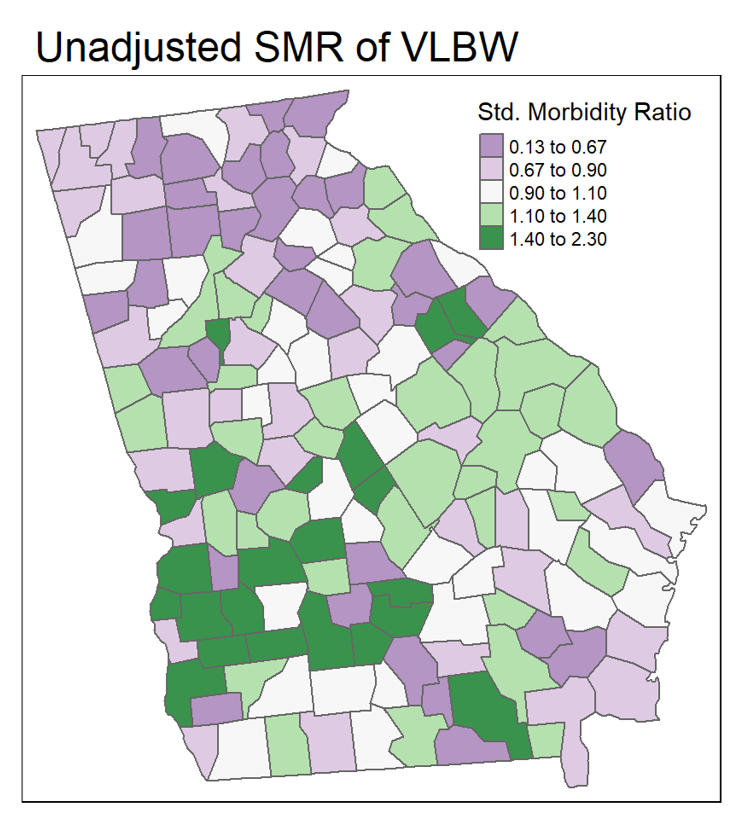
\includegraphics[width=0.5\linewidth]{images/diverge-smr} \caption{Mapping ratio measure with divergent palette}\label{fig:unnamed-chunk-32}
\end{figure}

In the map above, the SMR (a ratio of the county-specific prevalence of very low birth weight infants to the overall statewide live birth prevalence) varies from \(0.13\) to \(2.30\). But this range is not sequential in the same way as a \emph{risk} or \emph{prevalence}. Instead the neutral color is assigned to counties in the range of \(0.90-1.10\), around the null. This is a way of indicating these counties are \emph{average} or \emph{typical}. In contrast, counties with increasing \emph{excess morbidity} have darker green, and substantially \emph{lower morbidity} are darker purple.

\hypertarget{qualitative-palettes}{%
\subsubsection{Qualitative palettes}\label{qualitative-palettes}}

Qualitative refers to categories that are not naturally ordered or sequential. For instance if counties were assigned values for the single leading cause of death in the county, we might choose a qualitative palette, as a sequential or diverging palette might mislead the viewer into thinking there is some natural ordering to which causes should be more or less intense in their color.

\hypertarget{choropleth-binning-styles}{%
\subsection{Choropleth binning styles}\label{choropleth-binning-styles}}

A second topic relevant to the intersection of \emph{cartography} and \emph{epidemiologic thinking} is the means by which we choose cutpoints for visualizing data. In other words for a map to visually represent some underlying statistical value, we have to assign or map numerical values to colors. How you do that depends greatly on the intended message or story your map needs to tell. Are you interested in distinguish units that rank higher or lower in values? Or are you primarily focused on finding extreme outliers, with variation in the `\emph{middle}' of the distribution of less interest? These distinct purposes give rise to different decisions about how to assign colors to numerical values in your data.

\begin{figure}
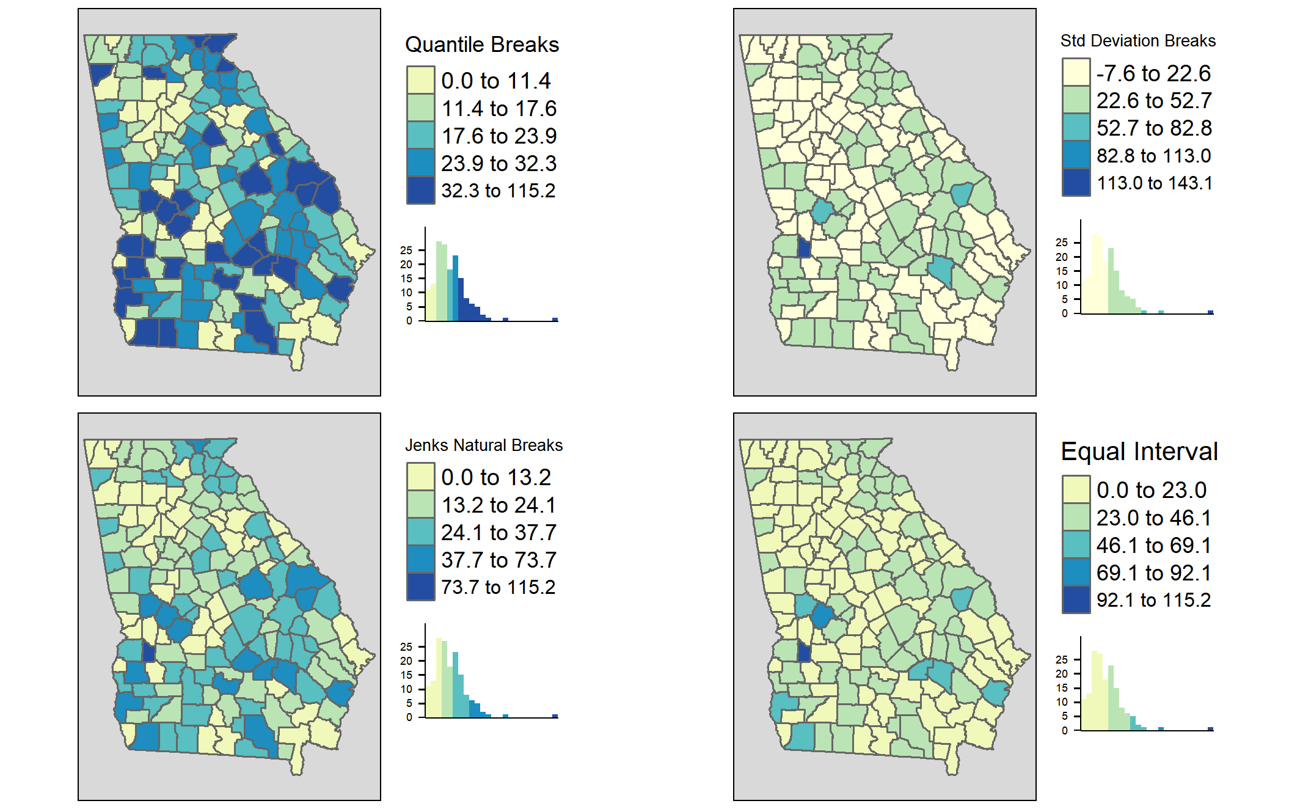
\includegraphics[width=0.75\linewidth]{images/cutpoints-vlbw} \caption{Comparing binning styles with same data}\label{fig:unnamed-chunk-33}
\end{figure}

As discussed in the lecture, there are numerous methods or styles for categorizing continuous data for choropleth mapping (e.g.~identical data is summarized under four different styles in figure above). Cynthia Brewer (of \href{https://colorbrewer2.org/\#type=sequential\&scheme=BuGn\&n=3}{ColorBrewer} fame) and Linda Pickle \citeyearpar{brewer_evaluation_2002} sought to evaluate which styles are most effective for communicating the spatial patterns of epidemiologic data.

As cartographers, Brewer \& Pickle were critical of the epidemiologists' over-reliance on quantile cutpoints, given many other strategies that seemed to have cartographic advantages. However, after randomizing map `\emph{readers}' to interpret maps of the same underlying epidemiologic data using \emph{seven different styles}, they determined that readers could most accurately and reliably interpret the disease patterns in maps using \emph{quantile cutpoints}. While there are benefits of the other styles for some purposes, for the common use of communicating which spatial areas \emph{rank higher or lower} in terms of disease burden, quantiles are most straightforward.

\hypertarget{mapping-time-series}{%
\subsubsection{Mapping time series}\label{mapping-time-series}}

It is common in spatial epidemiology that we want to map the spatial patterns of disease for several different snapshots in time as a series to observe the evolution of disease burden over time. But changing patterns over time raises additional questions about how to make cuts to the data. There are several options for determining the cutpoints when you have a time series:

\begin{enumerate}
\def\labelenumi{\arabic{enumi}.}
\tightlist
\item
  Pool all of the years data together before calculating the cutpoints (e.g.~using quantiles). Use the pooled cutpoints for all years.
\item
  Create custom year-specific cutpoints that reflect the distribution of data for each year separately.
\item
  Create cutpoints based on a single year and apply them to all other years.
\end{enumerate}

\begin{figure}
\centering
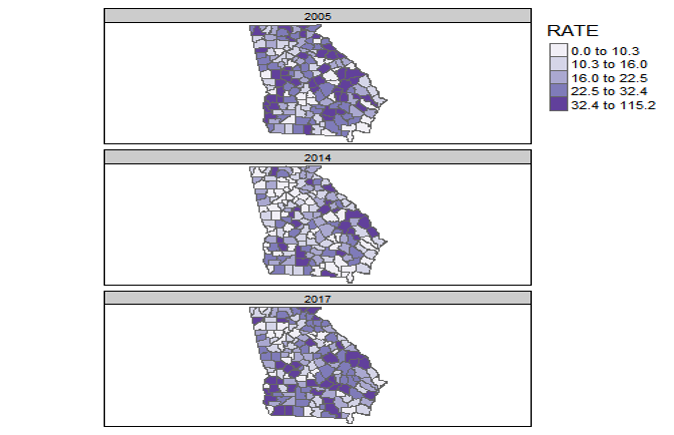
\includegraphics{images/time-series-ga-same-cuts.png}
\caption{\label{fig:unnamed-chunk-34}Georgia MVC deaths by year with a common scale}
\end{figure}

The map above of Georgia motor vehicle crash mortality data in three different years (2005, 2014, 2017), was created in \passthrough{\lstinline!tmap!} using the \passthrough{\lstinline!tm\_facet()!} option where the the \passthrough{\lstinline!by =!} was year. As a result, the quantile cutpoints represent the breaks \emph{pooling all observations across the three years}. In other words the cutpoints come from 159 counties times three years: 477 values.

By having a common legend that applies to all three maps, this strategy is useful for comparing \emph{differences in absolute rates} across years.

\begin{figure}
\centering
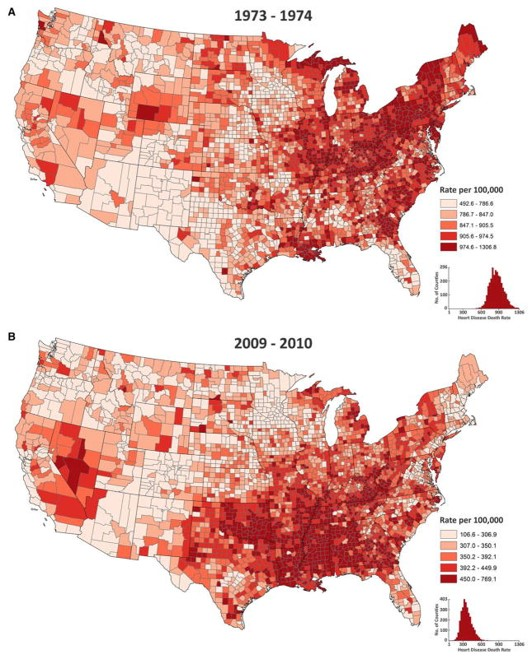
\includegraphics{images/time-series-us-quantiles.jpg}
\caption{\label{fig:unnamed-chunk-35}U.S. heart disease mortality with a year-specific scales}
\end{figure}

The map above of heart disease mortality rates by county in two years (1973-4; 2009-10) uses quantile breaks calculated \emph{separately for each time period}. This was done in part because the heart disease mortality rate declined so much between these years that a scale that distinguished highs from lows on one map would not distinguish anything on the other map. In this case what is being compared is not the \emph{absolute rates} but the \emph{relative ranking of counties} in the two years.

\hypertarget{spatial-analysis-in-epidemiology-w2}{%
\section{Spatial Analysis in Epidemiology, w2}\label{spatial-analysis-in-epidemiology-w2}}

Every spatial epidemiology project must include attention to data acquisition, cleaning, integration, and visualization. The specific workflow is driven largely by the overarching epidemiologic question, purpose, or goal. In this section we use a specific question to illustrate key steps to data preparation for epidemiologic cartography.

\begin{quote}
\textbf{Case Example Objective}: Create a choropleth map visualizing geographic variation in the all-cause mortality rate for U.S. counties in 2016-2018. Compare this to a choropleth map of \% uninsured in U.S. counties.
\end{quote}

This objective will be directly relevant for the lab this week as well as for the \emph{Visualizing US Mortality, Visual Portfolio}, an assignment due later in the semester.

Although this specific question dictates specific data needs, these four types of data are frequently needed to produce a map of a health outcome or state:

\begin{enumerate}
\def\labelenumi{\arabic{enumi}.}
\tightlist
\item
  Numerator data, in this case representing the count of deaths per county in the target year
\item
  Denominator data, in this case representing the population at risk for death in each county in the target year
\item
  Contextual or covariate data, in this case the prevalence uninsured for each U.S. county
\item
  Geometric data representing the shapes and boundaries of U.S. counties
\end{enumerate}

\hypertarget{obtaining-and-preparing-numerator-data}{%
\subsection{Obtaining and preparing numerator data}\label{obtaining-and-preparing-numerator-data}}

The event of interest (e.g.~the numerator in a risk, rate, or prevalence) can come from many sources. If you are conducting primary data collection, it arises from your study design and measurement. When using secondary data, it is common to use surveillance data (e.g.~vital records, notifiable diseases, registries, etc) or administrative data as a source of health events.

When using secondary data sources owned or managed by another entity, one challenge that can occur is \emph{suppression of data} to protect privacy. For example the National Center for Health Statistics mortality data available from \href{https://wonder.cdc.gov/}{CDC WONDER} suppresses the count of deaths, as well as the crude mortality rate, whenever the \emph{numerator count is less than ten events}. There can also be instances when a local or state public health agency fails to report data to NCHS, producing missing values.

\begin{rmdcaution}
Depending on the data format, it is possible that either \textbf{missing} or \textbf{suppressed} data could be inadvertently imported into R as \emph{zero-count} rather than missing. It is therefore critically important to understand the data source and guidelines. The decision about how to manage zero, missing, and suppressed data is an epidemiologic choice, but one that must be addressed \emph{before creating a map}.\\
\end{rmdcaution}

\begin{rmdtip}
\textbf{How to deal with data suppression}. There are many reasons your target data may fall below thresholds for suppressions. Perhaps the outcome event is quite rare, or you are stratifying by multiple demographic factors, or perhaps you are counting at a very small geographic unit. If suppression is problematic for mapping, consider pooling over multiple years, reducing demographic stratification, or using larger geographic areas to increase event count and reduce the number of suppressed cells.
\end{rmdtip}

For this example, we have downloaded all-cause mortality counts by county from CDC WONDER for 2016-2018 (pooling over three years to reduce suppression). In Lab we will discuss the procedure for acquiring data from the web. After importing the data this is how it appears.

\begin{lstlisting}[language=R]
head(death)
\end{lstlisting}

 
  \providecommand{\huxb}[2]{\arrayrulecolor[RGB]{#1}\global\arrayrulewidth=#2pt}
  \providecommand{\huxvb}[2]{\color[RGB]{#1}\vrule width #2pt}
  \providecommand{\huxtpad}[1]{\rule{0pt}{#1}}
  \providecommand{\huxbpad}[1]{\rule[-#1]{0pt}{#1}}

\begin{table}[ht]
\begin{centerbox}
\begin{threeparttable}
\captionsetup{justification=centering,singlelinecheck=off}
\caption{\label{tab:unnamed-chunk-39} }
 \setlength{\tabcolsep}{0pt}
\begin{tabular}{l l l l l}


\hhline{>{\huxb{0, 0, 0}{0.4}}->{\huxb{0, 0, 0}{0.4}}->{\huxb{0, 0, 0}{0.4}}->{\huxb{0, 0, 0}{0.4}}->{\huxb{0, 0, 0}{0.4}}-}
\arrayrulecolor{black}

\multicolumn{1}{!{\huxvb{0, 0, 0}{0.4}}l!{\huxvb{0, 0, 0}{0}}}{\huxtpad{6pt + 1em}\raggedright \hspace{6pt} \textbf{FIPS} \hspace{6pt}\huxbpad{6pt}} &
\multicolumn{1}{l!{\huxvb{0, 0, 0}{0}}}{\huxtpad{6pt + 1em}\raggedright \hspace{6pt} \textbf{County} \hspace{6pt}\huxbpad{6pt}} &
\multicolumn{1}{r!{\huxvb{0, 0, 0}{0}}}{\huxtpad{6pt + 1em}\raggedleft \hspace{6pt} \textbf{Deaths} \hspace{6pt}\huxbpad{6pt}} &
\multicolumn{1}{r!{\huxvb{0, 0, 0}{0}}}{\huxtpad{6pt + 1em}\raggedleft \hspace{6pt} \textbf{Population} \hspace{6pt}\huxbpad{6pt}} &
\multicolumn{1}{r!{\huxvb{0, 0, 0}{0.4}}}{\huxtpad{6pt + 1em}\raggedleft \hspace{6pt} \textbf{crude} \hspace{6pt}\huxbpad{6pt}} \tabularnewline[-0.5pt]


\hhline{>{\huxb{0, 0, 0}{0.4}}->{\huxb{0, 0, 0}{0.4}}->{\huxb{0, 0, 0}{0.4}}->{\huxb{0, 0, 0}{0.4}}->{\huxb{0, 0, 0}{0.4}}-}
\arrayrulecolor{black}

\multicolumn{1}{!{\huxvb{0, 0, 0}{0.4}}l!{\huxvb{0, 0, 0}{0}}}{\cellcolor[RGB]{242, 242, 242}\huxtpad{6pt + 1em}\raggedright \hspace{6pt} 01001 \hspace{6pt}\huxbpad{6pt}} &
\multicolumn{1}{l!{\huxvb{0, 0, 0}{0}}}{\cellcolor[RGB]{242, 242, 242}\huxtpad{6pt + 1em}\raggedright \hspace{6pt} Autauga County, AL \hspace{6pt}\huxbpad{6pt}} &
\multicolumn{1}{r!{\huxvb{0, 0, 0}{0}}}{\cellcolor[RGB]{242, 242, 242}\huxtpad{6pt + 1em}\raggedleft \hspace{6pt} 536 \hspace{6pt}\huxbpad{6pt}} &
\multicolumn{1}{r!{\huxvb{0, 0, 0}{0}}}{\cellcolor[RGB]{242, 242, 242}\huxtpad{6pt + 1em}\raggedleft \hspace{6pt} 55601 \hspace{6pt}\huxbpad{6pt}} &
\multicolumn{1}{r!{\huxvb{0, 0, 0}{0.4}}}{\cellcolor[RGB]{242, 242, 242}\huxtpad{6pt + 1em}\raggedleft \hspace{6pt} 964~~~~~~~ \hspace{6pt}\huxbpad{6pt}} \tabularnewline[-0.5pt]


\hhline{>{\huxb{0, 0, 0}{0.4}}|>{\huxb{0, 0, 0}{0.4}}|}
\arrayrulecolor{black}

\multicolumn{1}{!{\huxvb{0, 0, 0}{0.4}}l!{\huxvb{0, 0, 0}{0}}}{\huxtpad{6pt + 1em}\raggedright \hspace{6pt} 01003 \hspace{6pt}\huxbpad{6pt}} &
\multicolumn{1}{l!{\huxvb{0, 0, 0}{0}}}{\huxtpad{6pt + 1em}\raggedright \hspace{6pt} Baldwin County, AL \hspace{6pt}\huxbpad{6pt}} &
\multicolumn{1}{r!{\huxvb{0, 0, 0}{0}}}{\huxtpad{6pt + 1em}\raggedleft \hspace{6pt} 2357 \hspace{6pt}\huxbpad{6pt}} &
\multicolumn{1}{r!{\huxvb{0, 0, 0}{0}}}{\huxtpad{6pt + 1em}\raggedleft \hspace{6pt} 218022 \hspace{6pt}\huxbpad{6pt}} &
\multicolumn{1}{r!{\huxvb{0, 0, 0}{0.4}}}{\huxtpad{6pt + 1em}\raggedleft \hspace{6pt} 1.08e+03 \hspace{6pt}\huxbpad{6pt}} \tabularnewline[-0.5pt]


\hhline{>{\huxb{0, 0, 0}{0.4}}|>{\huxb{0, 0, 0}{0.4}}|}
\arrayrulecolor{black}

\multicolumn{1}{!{\huxvb{0, 0, 0}{0.4}}l!{\huxvb{0, 0, 0}{0}}}{\cellcolor[RGB]{242, 242, 242}\huxtpad{6pt + 1em}\raggedright \hspace{6pt} 01005 \hspace{6pt}\huxbpad{6pt}} &
\multicolumn{1}{l!{\huxvb{0, 0, 0}{0}}}{\cellcolor[RGB]{242, 242, 242}\huxtpad{6pt + 1em}\raggedright \hspace{6pt} Barbour County, AL \hspace{6pt}\huxbpad{6pt}} &
\multicolumn{1}{r!{\huxvb{0, 0, 0}{0}}}{\cellcolor[RGB]{242, 242, 242}\huxtpad{6pt + 1em}\raggedleft \hspace{6pt} 312 \hspace{6pt}\huxbpad{6pt}} &
\multicolumn{1}{r!{\huxvb{0, 0, 0}{0}}}{\cellcolor[RGB]{242, 242, 242}\huxtpad{6pt + 1em}\raggedleft \hspace{6pt} 24881 \hspace{6pt}\huxbpad{6pt}} &
\multicolumn{1}{r!{\huxvb{0, 0, 0}{0.4}}}{\cellcolor[RGB]{242, 242, 242}\huxtpad{6pt + 1em}\raggedleft \hspace{6pt} 1.25e+03 \hspace{6pt}\huxbpad{6pt}} \tabularnewline[-0.5pt]


\hhline{>{\huxb{0, 0, 0}{0.4}}|>{\huxb{0, 0, 0}{0.4}}|}
\arrayrulecolor{black}

\multicolumn{1}{!{\huxvb{0, 0, 0}{0.4}}l!{\huxvb{0, 0, 0}{0}}}{\huxtpad{6pt + 1em}\raggedright \hspace{6pt} 01007 \hspace{6pt}\huxbpad{6pt}} &
\multicolumn{1}{l!{\huxvb{0, 0, 0}{0}}}{\huxtpad{6pt + 1em}\raggedright \hspace{6pt} Bibb County, AL \hspace{6pt}\huxbpad{6pt}} &
\multicolumn{1}{r!{\huxvb{0, 0, 0}{0}}}{\huxtpad{6pt + 1em}\raggedleft \hspace{6pt} 276 \hspace{6pt}\huxbpad{6pt}} &
\multicolumn{1}{r!{\huxvb{0, 0, 0}{0}}}{\huxtpad{6pt + 1em}\raggedleft \hspace{6pt} 22400 \hspace{6pt}\huxbpad{6pt}} &
\multicolumn{1}{r!{\huxvb{0, 0, 0}{0.4}}}{\huxtpad{6pt + 1em}\raggedleft \hspace{6pt} 1.23e+03 \hspace{6pt}\huxbpad{6pt}} \tabularnewline[-0.5pt]


\hhline{>{\huxb{0, 0, 0}{0.4}}|>{\huxb{0, 0, 0}{0.4}}|}
\arrayrulecolor{black}

\multicolumn{1}{!{\huxvb{0, 0, 0}{0.4}}l!{\huxvb{0, 0, 0}{0}}}{\cellcolor[RGB]{242, 242, 242}\huxtpad{6pt + 1em}\raggedright \hspace{6pt} 01009 \hspace{6pt}\huxbpad{6pt}} &
\multicolumn{1}{l!{\huxvb{0, 0, 0}{0}}}{\cellcolor[RGB]{242, 242, 242}\huxtpad{6pt + 1em}\raggedright \hspace{6pt} Blount County, AL \hspace{6pt}\huxbpad{6pt}} &
\multicolumn{1}{r!{\huxvb{0, 0, 0}{0}}}{\cellcolor[RGB]{242, 242, 242}\huxtpad{6pt + 1em}\raggedleft \hspace{6pt} 689 \hspace{6pt}\huxbpad{6pt}} &
\multicolumn{1}{r!{\huxvb{0, 0, 0}{0}}}{\cellcolor[RGB]{242, 242, 242}\huxtpad{6pt + 1em}\raggedleft \hspace{6pt} 57840 \hspace{6pt}\huxbpad{6pt}} &
\multicolumn{1}{r!{\huxvb{0, 0, 0}{0.4}}}{\cellcolor[RGB]{242, 242, 242}\huxtpad{6pt + 1em}\raggedleft \hspace{6pt} 1.19e+03 \hspace{6pt}\huxbpad{6pt}} \tabularnewline[-0.5pt]


\hhline{>{\huxb{0, 0, 0}{0.4}}|>{\huxb{0, 0, 0}{0.4}}|}
\arrayrulecolor{black}

\multicolumn{1}{!{\huxvb{0, 0, 0}{0.4}}l!{\huxvb{0, 0, 0}{0}}}{\huxtpad{6pt + 1em}\raggedright \hspace{6pt} 01011 \hspace{6pt}\huxbpad{6pt}} &
\multicolumn{1}{l!{\huxvb{0, 0, 0}{0}}}{\huxtpad{6pt + 1em}\raggedright \hspace{6pt} Bullock County, AL \hspace{6pt}\huxbpad{6pt}} &
\multicolumn{1}{r!{\huxvb{0, 0, 0}{0}}}{\huxtpad{6pt + 1em}\raggedleft \hspace{6pt} 112 \hspace{6pt}\huxbpad{6pt}} &
\multicolumn{1}{r!{\huxvb{0, 0, 0}{0}}}{\huxtpad{6pt + 1em}\raggedleft \hspace{6pt} 10138 \hspace{6pt}\huxbpad{6pt}} &
\multicolumn{1}{r!{\huxvb{0, 0, 0}{0.4}}}{\huxtpad{6pt + 1em}\raggedleft \hspace{6pt} 1.1e+03~ \hspace{6pt}\huxbpad{6pt}} \tabularnewline[-0.5pt]


\hhline{>{\huxb{0, 0, 0}{0.4}}->{\huxb{0, 0, 0}{0.4}}->{\huxb{0, 0, 0}{0.4}}->{\huxb{0, 0, 0}{0.4}}->{\huxb{0, 0, 0}{0.4}}-}
\arrayrulecolor{black}
\end{tabular}
\end{threeparttable}\par\end{centerbox}

\end{table}
 

\hypertarget{obtaining-and-preparing-denominator-or-contextual-data}{%
\subsection{Obtaining and preparing denominator or contextual data}\label{obtaining-and-preparing-denominator-or-contextual-data}}

The mortality data accessed from CDC included both numerator (count of deaths) and denominator (population at risk). However there are instances where you may have one dataset that provides the health event data (numerator), but you need to link it to a population denominator in order to calculate risk, rate, or prevalence. The U.S. Census Bureau maintains the most reliable population count data for the U.S., and it is available in aggregates from Census Block Group, Census Tract, Zip code tabluation area, City or Place, County, State, and Region.

Census data can be aggregated as total population or stratified by age, gender, race/ethnicity, and many other variables. The census data also contains measures of social, economic, and housing attributes which may be relevant has \emph{context} or \emph{exposures} in spatial epidemiologic analyses. There are two broad types of data demographic and socioeconomic data released by the Census Bureau.

\begin{itemize}
\tightlist
\item
  \textbf{Decennial Census} tables which (theoretically) count 100\% of the population every 10 years. These can be cross-classified by age, race/ethnicity, sex, and householder status (e.g.~whether head of house owns or rents and how many people live in house)
\item
  \textbf{\href{https://www.census.gov/programs-surveys/acs}{American Community Survey (ACS)}} tables which provide a much larger number of measures but are based on samples rather than complete counts. The ACS began in the early 2000's and is a continually sampled survey. Despite being collected every year, for many small areas (e.g.~census tracts or even counties) there are not enough responses in a single year to make reliable estimates. Therefore ACS data pooled into 5-year moving-window datasets. For instance the 2014-2018 ACS (the most recent release) reports estimates for all responses collected during that time period, and these are available from the Census Block Group up. The next release will probably come in late 2020, and will be for 2015-2019.
\end{itemize}

You may have accessed Census or ACS data directly from the Census Bureau website for other classes or tasks in the past. In the interest of \emph{reproducibility} and efficiency, we introduce the \passthrough{\lstinline!tidycensus!} package in \passthrough{\lstinline!R!}. It is an excellent tool for acquiring either Decennial Census or ACS data directly within \passthrough{\lstinline!R!}. The advantage of doing so is twofold: first it can be quicker once you learn how to do it; second, it makes your data acquisition fully reproducible without any unrecorded steps happening in web browsers.

\begin{rmdnote}
We will practice the code in the next few sections in lab. It is included here as a primer. In these sections I walk through \textbf{one way} to download and prepare data to quantify the county-level prevalence of the population who are uninsured, as this might be a covariate of interest when examining spatial variation in mortality. I selected the code below because it is \emph{relatively} efficient, although you may find some of it complex or confusing. I include it for those who would like to explore other data-manipulation functions in \passthrough{\lstinline!R!}. Please note that you do not need learn all of the functions in this Census data acquisitions section below for this course, although you might find these or related approaches useful. Note also that there are many ways to accomplish anything in \passthrough{\lstinline!R!}, and you could achieve the same ends with different strategies.
\end{rmdnote}

\hypertarget{setting-up-census-api}{%
\subsubsection{Setting up Census API}\label{setting-up-census-api}}

To access any Census products (e.g.~attribute tables or geographic boundary files) using the \passthrough{\lstinline!tidycensus!} package, you need to \emph{register} yourself by declaring your API key. If you haven't already done so, \href{https://api.census.gov/data/key_signup.html}{go here to register for the key}.

\begin{lstlisting}[language=R]
# Only do this if you haven't already done it; it should only need to be done once.

tidycensus::census_api_key('YourKeyHere', install = T) 
\end{lstlisting}

\hypertarget{choosing-variables}{%
\subsubsection{Choosing Variables}\label{choosing-variables}}

By far the biggest challenge of requesting data from the Census Bureau is knowing \emph{what you want}, and \emph{where it is stored}. Census data are distributed as aggregated counts contained in \emph{specific tables} (each has a unique ID), and made up of \emph{specific variables} (also a unique ID composed of table ID plus a unique ID). There are two ways to find variables:

\begin{itemize}
\tightlist
\item
  You could go to the Census website and browse around. For instance the \href{https://data.census.gov/cedsci/}{Census Data Explorer website} is one way to browse the topics and variables
\item
  You could download all of the variables for a given year into \passthrough{\lstinline!R!}, and use filters to search it.
\end{itemize}

This code queries the Census website (assuming you have internet connection) and requests a list of all variables for the ACS 5-year pooled dataset (e.g.~\passthrough{\lstinline!acs5!}) and for the window of time ending in 2018 (e.g.~2014-2018). I also specify \passthrough{\lstinline!cache = T!} which just means to save the results for quicker loading if I ask again in the future.

\begin{lstlisting}[language=R]
library(tidycensus)

all_vars <- load_variables(year = 2018, dataset = 'acs5', cache = T)

head(all_vars)
\end{lstlisting}

It may be easiest to look at the dataset using the \passthrough{\lstinline!View()!} function. When you do so, you see the three variables, and you have the option to click the \textbf{Filter} button (upper left of View pane; looks like a funnel). The \emph{Filter} option is one way to search key words in either the \passthrough{\lstinline!label!} or \passthrough{\lstinline!concept!} column.

We are interested in capturing the prevalence of uninsured in each county. Try this:

\begin{itemize}
\tightlist
\item
  Go to View mode of variables (e.g.~\passthrough{\lstinline!View(all\_vars)!})
\item
  Click the \emph{Filter} button
\item
  Type \passthrough{\lstinline!insurance!} in the \passthrough{\lstinline!concept!} field
\item
  Type \passthrough{\lstinline!B27001!} in the \passthrough{\lstinline!name!} field
\end{itemize}

\begin{figure}
\centering
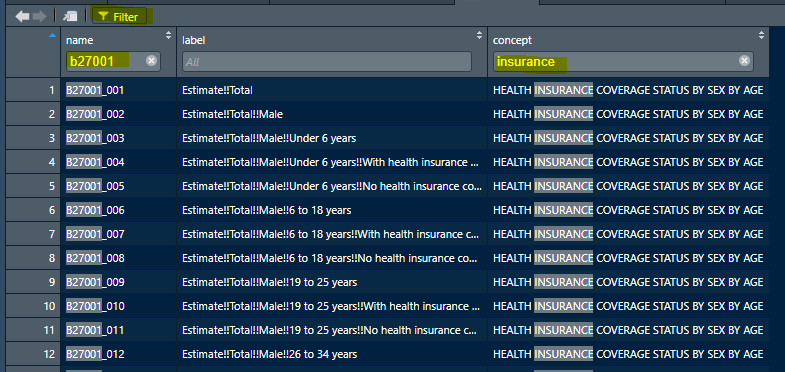
\includegraphics{images/acs-var-view.PNG}
\caption{\label{fig:unnamed-chunk-43}Screenshot of RStudio View() of ACS variables}
\end{figure}

What we want is a list of the specific tables and variable ID's to extract from the Census. In lab we will use some more detailed code to accomplish this goal.

You may have noticed that the full list of ACS variables has nearly 27,000 variables! In the code below I use some tricks to filter the huge list of all variables to get only the names I want. It relies on the \passthrough{\lstinline!tidyverse!} package \passthrough{\lstinline!stringr!} which is great for manipulating character variables (this is great for many data science tasks; \href{https://stringr.tidyverse.org/}{read more about \passthrough{\lstinline!stringr!} here}). In this case I am using it to filter down to just the table I want (e.g.~\passthrough{\lstinline!B27001!}), and then to get the names of the variables that contain the string \emph{`No health insurance'}.

Here is the list of variables we want to acquire; each one represents a count of uninsured at each of multiple age groups. We will sum them up to get a total population uninsured prevalence.

\begin{lstlisting}
##  [1] "B27001_001" "B27001_005" "B27001_008" "B27001_011" "B27001_014"
##  [6] "B27001_017" "B27001_020" "B27001_023" "B27001_026" "B27001_029"
## [11] "B27001_033" "B27001_036" "B27001_039" "B27001_042" "B27001_045"
## [16] "B27001_048" "B27001_051" "B27001_054" "B27001_057"
\end{lstlisting}

\hypertarget{retrieving-data-from-census}{%
\subsubsection{Retrieving data from Census}\label{retrieving-data-from-census}}

To actually retrieve data from the Census we use the function \passthrough{\lstinline!get\_acs()!} (or if you were getting decennial data the function would be \passthrough{\lstinline!get\_decennial()!}). When you request data you must specify the geography (e.g.~do you want counts for states, counties, census tracts, census block groups?), the variables, the year, and the dataset. Look at \passthrough{\lstinline!?get\_acs!} to read more about options.

The following code chunks use the \passthrough{\lstinline!dplyr!} and \passthrough{\lstinline!tidyvrse!} verbs and the \passthrough{\lstinline!\%>\%!} (pipe) to connect data steps together. This is complex at first, but it is worth carefully examining how each step works. If you are not familiar with this syntax, it would probably be helpful to \protect\hyperlink{dplyr}{review the Appendix section on \passthrough{\lstinline!dplyr!}}.

\begin{lstlisting}[language=R]
# First, request the data from ACS
insure_tidy <- get_acs(geography = 'county',
                     variables = myVars,
                     year = 2018, 
                     survey = 'acs5') %>%
  select(-moe)

# Look at the resulting object
head(insure_tidy)
\end{lstlisting}

 
  \providecommand{\huxb}[2]{\arrayrulecolor[RGB]{#1}\global\arrayrulewidth=#2pt}
  \providecommand{\huxvb}[2]{\color[RGB]{#1}\vrule width #2pt}
  \providecommand{\huxtpad}[1]{\rule{0pt}{#1}}
  \providecommand{\huxbpad}[1]{\rule[-#1]{0pt}{#1}}

\begin{table}[ht]
\begin{centerbox}
\begin{threeparttable}
\captionsetup{justification=centering,singlelinecheck=off}
\caption{\label{tab:unnamed-chunk-46} }
 \setlength{\tabcolsep}{0pt}
\begin{tabular}{l l l l}


\hhline{>{\huxb{0, 0, 0}{0.4}}->{\huxb{0, 0, 0}{0.4}}->{\huxb{0, 0, 0}{0.4}}->{\huxb{0, 0, 0}{0.4}}-}
\arrayrulecolor{black}

\multicolumn{1}{!{\huxvb{0, 0, 0}{0.4}}l!{\huxvb{0, 0, 0}{0}}}{\huxtpad{6pt + 1em}\raggedright \hspace{6pt} \textbf{GEOID} \hspace{6pt}\huxbpad{6pt}} &
\multicolumn{1}{l!{\huxvb{0, 0, 0}{0}}}{\huxtpad{6pt + 1em}\raggedright \hspace{6pt} \textbf{NAME} \hspace{6pt}\huxbpad{6pt}} &
\multicolumn{1}{l!{\huxvb{0, 0, 0}{0}}}{\huxtpad{6pt + 1em}\raggedright \hspace{6pt} \textbf{variable} \hspace{6pt}\huxbpad{6pt}} &
\multicolumn{1}{r!{\huxvb{0, 0, 0}{0.4}}}{\huxtpad{6pt + 1em}\raggedleft \hspace{6pt} \textbf{estimate} \hspace{6pt}\huxbpad{6pt}} \tabularnewline[-0.5pt]


\hhline{>{\huxb{0, 0, 0}{0.4}}->{\huxb{0, 0, 0}{0.4}}->{\huxb{0, 0, 0}{0.4}}->{\huxb{0, 0, 0}{0.4}}-}
\arrayrulecolor{black}

\multicolumn{1}{!{\huxvb{0, 0, 0}{0.4}}l!{\huxvb{0, 0, 0}{0}}}{\cellcolor[RGB]{242, 242, 242}\huxtpad{6pt + 1em}\raggedright \hspace{6pt} 01001 \hspace{6pt}\huxbpad{6pt}} &
\multicolumn{1}{l!{\huxvb{0, 0, 0}{0}}}{\cellcolor[RGB]{242, 242, 242}\huxtpad{6pt + 1em}\raggedright \hspace{6pt} Autauga County, Alabama \hspace{6pt}\huxbpad{6pt}} &
\multicolumn{1}{l!{\huxvb{0, 0, 0}{0}}}{\cellcolor[RGB]{242, 242, 242}\huxtpad{6pt + 1em}\raggedright \hspace{6pt} B27001\_001 \hspace{6pt}\huxbpad{6pt}} &
\multicolumn{1}{r!{\huxvb{0, 0, 0}{0.4}}}{\cellcolor[RGB]{242, 242, 242}\huxtpad{6pt + 1em}\raggedleft \hspace{6pt} 5.43e+04 \hspace{6pt}\huxbpad{6pt}} \tabularnewline[-0.5pt]


\hhline{>{\huxb{0, 0, 0}{0.4}}|>{\huxb{0, 0, 0}{0.4}}|}
\arrayrulecolor{black}

\multicolumn{1}{!{\huxvb{0, 0, 0}{0.4}}l!{\huxvb{0, 0, 0}{0}}}{\huxtpad{6pt + 1em}\raggedright \hspace{6pt} 01001 \hspace{6pt}\huxbpad{6pt}} &
\multicolumn{1}{l!{\huxvb{0, 0, 0}{0}}}{\huxtpad{6pt + 1em}\raggedright \hspace{6pt} Autauga County, Alabama \hspace{6pt}\huxbpad{6pt}} &
\multicolumn{1}{l!{\huxvb{0, 0, 0}{0}}}{\huxtpad{6pt + 1em}\raggedright \hspace{6pt} B27001\_005 \hspace{6pt}\huxbpad{6pt}} &
\multicolumn{1}{r!{\huxvb{0, 0, 0}{0.4}}}{\huxtpad{6pt + 1em}\raggedleft \hspace{6pt} 36~~~~~~~ \hspace{6pt}\huxbpad{6pt}} \tabularnewline[-0.5pt]


\hhline{>{\huxb{0, 0, 0}{0.4}}|>{\huxb{0, 0, 0}{0.4}}|}
\arrayrulecolor{black}

\multicolumn{1}{!{\huxvb{0, 0, 0}{0.4}}l!{\huxvb{0, 0, 0}{0}}}{\cellcolor[RGB]{242, 242, 242}\huxtpad{6pt + 1em}\raggedright \hspace{6pt} 01001 \hspace{6pt}\huxbpad{6pt}} &
\multicolumn{1}{l!{\huxvb{0, 0, 0}{0}}}{\cellcolor[RGB]{242, 242, 242}\huxtpad{6pt + 1em}\raggedright \hspace{6pt} Autauga County, Alabama \hspace{6pt}\huxbpad{6pt}} &
\multicolumn{1}{l!{\huxvb{0, 0, 0}{0}}}{\cellcolor[RGB]{242, 242, 242}\huxtpad{6pt + 1em}\raggedright \hspace{6pt} B27001\_008 \hspace{6pt}\huxbpad{6pt}} &
\multicolumn{1}{r!{\huxvb{0, 0, 0}{0.4}}}{\cellcolor[RGB]{242, 242, 242}\huxtpad{6pt + 1em}\raggedleft \hspace{6pt} 157~~~~~~~ \hspace{6pt}\huxbpad{6pt}} \tabularnewline[-0.5pt]


\hhline{>{\huxb{0, 0, 0}{0.4}}|>{\huxb{0, 0, 0}{0.4}}|}
\arrayrulecolor{black}

\multicolumn{1}{!{\huxvb{0, 0, 0}{0.4}}l!{\huxvb{0, 0, 0}{0}}}{\huxtpad{6pt + 1em}\raggedright \hspace{6pt} 01001 \hspace{6pt}\huxbpad{6pt}} &
\multicolumn{1}{l!{\huxvb{0, 0, 0}{0}}}{\huxtpad{6pt + 1em}\raggedright \hspace{6pt} Autauga County, Alabama \hspace{6pt}\huxbpad{6pt}} &
\multicolumn{1}{l!{\huxvb{0, 0, 0}{0}}}{\huxtpad{6pt + 1em}\raggedright \hspace{6pt} B27001\_011 \hspace{6pt}\huxbpad{6pt}} &
\multicolumn{1}{r!{\huxvb{0, 0, 0}{0.4}}}{\huxtpad{6pt + 1em}\raggedleft \hspace{6pt} 397~~~~~~~ \hspace{6pt}\huxbpad{6pt}} \tabularnewline[-0.5pt]


\hhline{>{\huxb{0, 0, 0}{0.4}}|>{\huxb{0, 0, 0}{0.4}}|}
\arrayrulecolor{black}

\multicolumn{1}{!{\huxvb{0, 0, 0}{0.4}}l!{\huxvb{0, 0, 0}{0}}}{\cellcolor[RGB]{242, 242, 242}\huxtpad{6pt + 1em}\raggedright \hspace{6pt} 01001 \hspace{6pt}\huxbpad{6pt}} &
\multicolumn{1}{l!{\huxvb{0, 0, 0}{0}}}{\cellcolor[RGB]{242, 242, 242}\huxtpad{6pt + 1em}\raggedright \hspace{6pt} Autauga County, Alabama \hspace{6pt}\huxbpad{6pt}} &
\multicolumn{1}{l!{\huxvb{0, 0, 0}{0}}}{\cellcolor[RGB]{242, 242, 242}\huxtpad{6pt + 1em}\raggedright \hspace{6pt} B27001\_014 \hspace{6pt}\huxbpad{6pt}} &
\multicolumn{1}{r!{\huxvb{0, 0, 0}{0.4}}}{\cellcolor[RGB]{242, 242, 242}\huxtpad{6pt + 1em}\raggedleft \hspace{6pt} 354~~~~~~~ \hspace{6pt}\huxbpad{6pt}} \tabularnewline[-0.5pt]


\hhline{>{\huxb{0, 0, 0}{0.4}}|>{\huxb{0, 0, 0}{0.4}}|}
\arrayrulecolor{black}

\multicolumn{1}{!{\huxvb{0, 0, 0}{0.4}}l!{\huxvb{0, 0, 0}{0}}}{\huxtpad{6pt + 1em}\raggedright \hspace{6pt} 01001 \hspace{6pt}\huxbpad{6pt}} &
\multicolumn{1}{l!{\huxvb{0, 0, 0}{0}}}{\huxtpad{6pt + 1em}\raggedright \hspace{6pt} Autauga County, Alabama \hspace{6pt}\huxbpad{6pt}} &
\multicolumn{1}{l!{\huxvb{0, 0, 0}{0}}}{\huxtpad{6pt + 1em}\raggedright \hspace{6pt} B27001\_017 \hspace{6pt}\huxbpad{6pt}} &
\multicolumn{1}{r!{\huxvb{0, 0, 0}{0.4}}}{\huxtpad{6pt + 1em}\raggedleft \hspace{6pt} 500~~~~~~~ \hspace{6pt}\huxbpad{6pt}} \tabularnewline[-0.5pt]


\hhline{>{\huxb{0, 0, 0}{0.4}}->{\huxb{0, 0, 0}{0.4}}->{\huxb{0, 0, 0}{0.4}}->{\huxb{0, 0, 0}{0.4}}-}
\arrayrulecolor{black}
\end{tabular}
\end{threeparttable}\par\end{centerbox}

\end{table}
 

Looking at the first few rows of the data object \passthrough{\lstinline!insure\_tidy!} above, you might be surprised that there is a column labeled \passthrough{\lstinline!variable!}, and the cells within that column are actually what we \emph{thought were the variable names}! That is because these data are structured in a \passthrough{\lstinline!tidy!} format, which happens to be \emph{long} not \emph{wide}. \protect\hyperlink{pivot_}{Read more about transposing data here}. In the following steps we will reshape this data to be more useful.

What this code does:

\begin{itemize}
\tightlist
\item
  define the \passthrough{\lstinline!geography =!} as county.
\item
  Specify the vector (previously created and named \passthrough{\lstinline!myVars!}) of variables to download
\item
  Specify the year of interest. Note that 2018 references the \emph{2014-2018} 5-year window
\item
  specify the survey, which will most often be \passthrough{\lstinline!acs5!}
\end{itemize}

\begin{lstlisting}[language=R]
# Now I pull out the denominator
insure_denom <- insure_tidy %>%
  filter(variable == 'B27001_001') %>%
  rename(TOTPOP = estimate) %>%
  select(-variable)

# Look at the resulting object
head(insure_denom)
\end{lstlisting}

 
  \providecommand{\huxb}[2]{\arrayrulecolor[RGB]{#1}\global\arrayrulewidth=#2pt}
  \providecommand{\huxvb}[2]{\color[RGB]{#1}\vrule width #2pt}
  \providecommand{\huxtpad}[1]{\rule{0pt}{#1}}
  \providecommand{\huxbpad}[1]{\rule[-#1]{0pt}{#1}}

\begin{table}[ht]
\begin{centerbox}
\begin{threeparttable}
\captionsetup{justification=centering,singlelinecheck=off}
\caption{\label{tab:unnamed-chunk-47} }
 \setlength{\tabcolsep}{0pt}
\begin{tabular}{l l l}


\hhline{>{\huxb{0, 0, 0}{0.4}}->{\huxb{0, 0, 0}{0.4}}->{\huxb{0, 0, 0}{0.4}}-}
\arrayrulecolor{black}

\multicolumn{1}{!{\huxvb{0, 0, 0}{0.4}}l!{\huxvb{0, 0, 0}{0}}}{\huxtpad{6pt + 1em}\raggedright \hspace{6pt} \textbf{GEOID} \hspace{6pt}\huxbpad{6pt}} &
\multicolumn{1}{l!{\huxvb{0, 0, 0}{0}}}{\huxtpad{6pt + 1em}\raggedright \hspace{6pt} \textbf{NAME} \hspace{6pt}\huxbpad{6pt}} &
\multicolumn{1}{r!{\huxvb{0, 0, 0}{0.4}}}{\huxtpad{6pt + 1em}\raggedleft \hspace{6pt} \textbf{TOTPOP} \hspace{6pt}\huxbpad{6pt}} \tabularnewline[-0.5pt]


\hhline{>{\huxb{0, 0, 0}{0.4}}->{\huxb{0, 0, 0}{0.4}}->{\huxb{0, 0, 0}{0.4}}-}
\arrayrulecolor{black}

\multicolumn{1}{!{\huxvb{0, 0, 0}{0.4}}l!{\huxvb{0, 0, 0}{0}}}{\cellcolor[RGB]{242, 242, 242}\huxtpad{6pt + 1em}\raggedright \hspace{6pt} 01001 \hspace{6pt}\huxbpad{6pt}} &
\multicolumn{1}{l!{\huxvb{0, 0, 0}{0}}}{\cellcolor[RGB]{242, 242, 242}\huxtpad{6pt + 1em}\raggedright \hspace{6pt} Autauga County, Alabama \hspace{6pt}\huxbpad{6pt}} &
\multicolumn{1}{r!{\huxvb{0, 0, 0}{0.4}}}{\cellcolor[RGB]{242, 242, 242}\huxtpad{6pt + 1em}\raggedleft \hspace{6pt} 5.43e+04 \hspace{6pt}\huxbpad{6pt}} \tabularnewline[-0.5pt]


\hhline{>{\huxb{0, 0, 0}{0.4}}|>{\huxb{0, 0, 0}{0.4}}|}
\arrayrulecolor{black}

\multicolumn{1}{!{\huxvb{0, 0, 0}{0.4}}l!{\huxvb{0, 0, 0}{0}}}{\huxtpad{6pt + 1em}\raggedright \hspace{6pt} 01003 \hspace{6pt}\huxbpad{6pt}} &
\multicolumn{1}{l!{\huxvb{0, 0, 0}{0}}}{\huxtpad{6pt + 1em}\raggedright \hspace{6pt} Baldwin County, Alabama \hspace{6pt}\huxbpad{6pt}} &
\multicolumn{1}{r!{\huxvb{0, 0, 0}{0.4}}}{\huxtpad{6pt + 1em}\raggedleft \hspace{6pt} 2.05e+05 \hspace{6pt}\huxbpad{6pt}} \tabularnewline[-0.5pt]


\hhline{>{\huxb{0, 0, 0}{0.4}}|>{\huxb{0, 0, 0}{0.4}}|}
\arrayrulecolor{black}

\multicolumn{1}{!{\huxvb{0, 0, 0}{0.4}}l!{\huxvb{0, 0, 0}{0}}}{\cellcolor[RGB]{242, 242, 242}\huxtpad{6pt + 1em}\raggedright \hspace{6pt} 01005 \hspace{6pt}\huxbpad{6pt}} &
\multicolumn{1}{l!{\huxvb{0, 0, 0}{0}}}{\cellcolor[RGB]{242, 242, 242}\huxtpad{6pt + 1em}\raggedright \hspace{6pt} Barbour County, Alabama \hspace{6pt}\huxbpad{6pt}} &
\multicolumn{1}{r!{\huxvb{0, 0, 0}{0.4}}}{\cellcolor[RGB]{242, 242, 242}\huxtpad{6pt + 1em}\raggedleft \hspace{6pt} 2.29e+04 \hspace{6pt}\huxbpad{6pt}} \tabularnewline[-0.5pt]


\hhline{>{\huxb{0, 0, 0}{0.4}}|>{\huxb{0, 0, 0}{0.4}}|}
\arrayrulecolor{black}

\multicolumn{1}{!{\huxvb{0, 0, 0}{0.4}}l!{\huxvb{0, 0, 0}{0}}}{\huxtpad{6pt + 1em}\raggedright \hspace{6pt} 01007 \hspace{6pt}\huxbpad{6pt}} &
\multicolumn{1}{l!{\huxvb{0, 0, 0}{0}}}{\huxtpad{6pt + 1em}\raggedright \hspace{6pt} Bibb County, Alabama \hspace{6pt}\huxbpad{6pt}} &
\multicolumn{1}{r!{\huxvb{0, 0, 0}{0.4}}}{\huxtpad{6pt + 1em}\raggedleft \hspace{6pt} 2.05e+04 \hspace{6pt}\huxbpad{6pt}} \tabularnewline[-0.5pt]


\hhline{>{\huxb{0, 0, 0}{0.4}}|>{\huxb{0, 0, 0}{0.4}}|}
\arrayrulecolor{black}

\multicolumn{1}{!{\huxvb{0, 0, 0}{0.4}}l!{\huxvb{0, 0, 0}{0}}}{\cellcolor[RGB]{242, 242, 242}\huxtpad{6pt + 1em}\raggedright \hspace{6pt} 01009 \hspace{6pt}\huxbpad{6pt}} &
\multicolumn{1}{l!{\huxvb{0, 0, 0}{0}}}{\cellcolor[RGB]{242, 242, 242}\huxtpad{6pt + 1em}\raggedright \hspace{6pt} Blount County, Alabama \hspace{6pt}\huxbpad{6pt}} &
\multicolumn{1}{r!{\huxvb{0, 0, 0}{0.4}}}{\cellcolor[RGB]{242, 242, 242}\huxtpad{6pt + 1em}\raggedleft \hspace{6pt} 5.72e+04 \hspace{6pt}\huxbpad{6pt}} \tabularnewline[-0.5pt]


\hhline{>{\huxb{0, 0, 0}{0.4}}|>{\huxb{0, 0, 0}{0.4}}|}
\arrayrulecolor{black}

\multicolumn{1}{!{\huxvb{0, 0, 0}{0.4}}l!{\huxvb{0, 0, 0}{0}}}{\huxtpad{6pt + 1em}\raggedright \hspace{6pt} 01011 \hspace{6pt}\huxbpad{6pt}} &
\multicolumn{1}{l!{\huxvb{0, 0, 0}{0}}}{\huxtpad{6pt + 1em}\raggedright \hspace{6pt} Bullock County, Alabama \hspace{6pt}\huxbpad{6pt}} &
\multicolumn{1}{r!{\huxvb{0, 0, 0}{0.4}}}{\huxtpad{6pt + 1em}\raggedleft \hspace{6pt} 9.98e+03 \hspace{6pt}\huxbpad{6pt}} \tabularnewline[-0.5pt]


\hhline{>{\huxb{0, 0, 0}{0.4}}->{\huxb{0, 0, 0}{0.4}}->{\huxb{0, 0, 0}{0.4}}-}
\arrayrulecolor{black}
\end{tabular}
\end{threeparttable}\par\end{centerbox}

\end{table}
 

The code above was necessary because most of the variables were age-specific counts of the number of uninsured people. But one variable, \passthrough{\lstinline!B27001\_001!} is the count of all included in the table. In other words, it is the \emph{denominator} for calculating the prevalence of uninsured. Therefore I did the following in the code above:

\begin{itemize}
\tightlist
\item
  \passthrough{\lstinline!filter()!} restricts to only the rows of data where the variable is the denominator count (B27001\_001). Filter is like \passthrough{\lstinline!where!} in SAS
\item
  \passthrough{\lstinline!rename()!} is a way to rename variables to my own liking
\item
  \passthrough{\lstinline!select()!} drops the variable called \passthrough{\lstinline!variable!}
\end{itemize}

\begin{lstlisting}[language=R]
# Now I sum up all the variables for the numerator
insure_num <- insure_tidy %>%
  filter(variable != 'B27001_001') %>%
  group_by(GEOID) %>%
  summarise(no_insure = sum(estimate))

head(insure_num)
\end{lstlisting}

 
  \providecommand{\huxb}[2]{\arrayrulecolor[RGB]{#1}\global\arrayrulewidth=#2pt}
  \providecommand{\huxvb}[2]{\color[RGB]{#1}\vrule width #2pt}
  \providecommand{\huxtpad}[1]{\rule{0pt}{#1}}
  \providecommand{\huxbpad}[1]{\rule[-#1]{0pt}{#1}}

\begin{table}[ht]
\begin{centerbox}
\begin{threeparttable}
\captionsetup{justification=centering,singlelinecheck=off}
\caption{\label{tab:unnamed-chunk-48} }
 \setlength{\tabcolsep}{0pt}
\begin{tabular}{l l}


\hhline{>{\huxb{0, 0, 0}{0.4}}->{\huxb{0, 0, 0}{0.4}}-}
\arrayrulecolor{black}

\multicolumn{1}{!{\huxvb{0, 0, 0}{0.4}}l!{\huxvb{0, 0, 0}{0}}}{\huxtpad{6pt + 1em}\raggedright \hspace{6pt} \textbf{GEOID} \hspace{6pt}\huxbpad{6pt}} &
\multicolumn{1}{r!{\huxvb{0, 0, 0}{0.4}}}{\huxtpad{6pt + 1em}\raggedleft \hspace{6pt} \textbf{no\_insure} \hspace{6pt}\huxbpad{6pt}} \tabularnewline[-0.5pt]


\hhline{>{\huxb{0, 0, 0}{0.4}}->{\huxb{0, 0, 0}{0.4}}-}
\arrayrulecolor{black}

\multicolumn{1}{!{\huxvb{0, 0, 0}{0.4}}l!{\huxvb{0, 0, 0}{0}}}{\cellcolor[RGB]{242, 242, 242}\huxtpad{6pt + 1em}\raggedright \hspace{6pt} 01001 \hspace{6pt}\huxbpad{6pt}} &
\multicolumn{1}{r!{\huxvb{0, 0, 0}{0.4}}}{\cellcolor[RGB]{242, 242, 242}\huxtpad{6pt + 1em}\raggedleft \hspace{6pt} 3.88e+03 \hspace{6pt}\huxbpad{6pt}} \tabularnewline[-0.5pt]


\hhline{>{\huxb{0, 0, 0}{0.4}}|>{\huxb{0, 0, 0}{0.4}}|}
\arrayrulecolor{black}

\multicolumn{1}{!{\huxvb{0, 0, 0}{0.4}}l!{\huxvb{0, 0, 0}{0}}}{\huxtpad{6pt + 1em}\raggedright \hspace{6pt} 01003 \hspace{6pt}\huxbpad{6pt}} &
\multicolumn{1}{r!{\huxvb{0, 0, 0}{0.4}}}{\huxtpad{6pt + 1em}\raggedleft \hspace{6pt} 2.09e+04 \hspace{6pt}\huxbpad{6pt}} \tabularnewline[-0.5pt]


\hhline{>{\huxb{0, 0, 0}{0.4}}|>{\huxb{0, 0, 0}{0.4}}|}
\arrayrulecolor{black}

\multicolumn{1}{!{\huxvb{0, 0, 0}{0.4}}l!{\huxvb{0, 0, 0}{0}}}{\cellcolor[RGB]{242, 242, 242}\huxtpad{6pt + 1em}\raggedright \hspace{6pt} 01005 \hspace{6pt}\huxbpad{6pt}} &
\multicolumn{1}{r!{\huxvb{0, 0, 0}{0.4}}}{\cellcolor[RGB]{242, 242, 242}\huxtpad{6pt + 1em}\raggedleft \hspace{6pt} 2.56e+03 \hspace{6pt}\huxbpad{6pt}} \tabularnewline[-0.5pt]


\hhline{>{\huxb{0, 0, 0}{0.4}}|>{\huxb{0, 0, 0}{0.4}}|}
\arrayrulecolor{black}

\multicolumn{1}{!{\huxvb{0, 0, 0}{0.4}}l!{\huxvb{0, 0, 0}{0}}}{\huxtpad{6pt + 1em}\raggedright \hspace{6pt} 01007 \hspace{6pt}\huxbpad{6pt}} &
\multicolumn{1}{r!{\huxvb{0, 0, 0}{0.4}}}{\huxtpad{6pt + 1em}\raggedleft \hspace{6pt} 1.62e+03 \hspace{6pt}\huxbpad{6pt}} \tabularnewline[-0.5pt]


\hhline{>{\huxb{0, 0, 0}{0.4}}|>{\huxb{0, 0, 0}{0.4}}|}
\arrayrulecolor{black}

\multicolumn{1}{!{\huxvb{0, 0, 0}{0.4}}l!{\huxvb{0, 0, 0}{0}}}{\cellcolor[RGB]{242, 242, 242}\huxtpad{6pt + 1em}\raggedright \hspace{6pt} 01009 \hspace{6pt}\huxbpad{6pt}} &
\multicolumn{1}{r!{\huxvb{0, 0, 0}{0.4}}}{\cellcolor[RGB]{242, 242, 242}\huxtpad{6pt + 1em}\raggedleft \hspace{6pt} 6.3e+03~ \hspace{6pt}\huxbpad{6pt}} \tabularnewline[-0.5pt]


\hhline{>{\huxb{0, 0, 0}{0.4}}|>{\huxb{0, 0, 0}{0.4}}|}
\arrayrulecolor{black}

\multicolumn{1}{!{\huxvb{0, 0, 0}{0.4}}l!{\huxvb{0, 0, 0}{0}}}{\huxtpad{6pt + 1em}\raggedright \hspace{6pt} 01011 \hspace{6pt}\huxbpad{6pt}} &
\multicolumn{1}{r!{\huxvb{0, 0, 0}{0.4}}}{\huxtpad{6pt + 1em}\raggedleft \hspace{6pt} 1.08e+03 \hspace{6pt}\huxbpad{6pt}} \tabularnewline[-0.5pt]


\hhline{>{\huxb{0, 0, 0}{0.4}}->{\huxb{0, 0, 0}{0.4}}-}
\arrayrulecolor{black}
\end{tabular}
\end{threeparttable}\par\end{centerbox}

\end{table}
 

The code above addresses an issue common to census tables: they may not be constructed in the way you want them. As discussed above, in this case the values are counts for each age group, but we only want a single count for the entire population of each county. Therefore, it is necessary to \emph{sum across} or \emph{aggregate} the counts over all age groups to get a single count (the numerator number of uninsured) for each county. The strategy used above was specific to the data being in \emph{long format}, which happens to be \passthrough{\lstinline!tidy!} data in this case. \protect\hyperlink{pivot_}{Read about changing between long and wide here}.

The code above achieves this through steps:

\begin{itemize}
\tightlist
\item
  \passthrough{\lstinline!filter()!} using the \passthrough{\lstinline"!="} mean ``\emph{is \textbf{not} equal to}''; this simply removes the denominator variable, so that we are only summing over numerator counts
\item
  \passthrough{\lstinline!group\_by()!} is a very useful \passthrough{\lstinline!dplyr!} verb; it is similar to using \passthrough{\lstinline!class!} in SAS, and tells \passthrough{\lstinline!R!} to do something separately for each group (e.g.~each \passthrough{\lstinline!GEOID!} or county in this case)
\item
  \passthrough{\lstinline!summarise()!} is a verb that works hand-in-hand with \passthrough{\lstinline!group\_by()!}. The grouping declares which groups, but the \passthrough{\lstinline!summarise()!} tells what to do. In this case we just want to count up all of those uninsured across all age gruops.
\end{itemize}

\begin{lstlisting}[language=R]
# Finally, merge the numerator and denominator in order to calculate prevalence
uninsured <- insure_denom %>%
  left_join(insure_num, by = 'GEOID') %>%
  mutate(uninsured = no_insure / TOTPOP) %>%
  select(GEOID, uninsured)

# Take a look at the resulting object
head(uninsured)
\end{lstlisting}

 
  \providecommand{\huxb}[2]{\arrayrulecolor[RGB]{#1}\global\arrayrulewidth=#2pt}
  \providecommand{\huxvb}[2]{\color[RGB]{#1}\vrule width #2pt}
  \providecommand{\huxtpad}[1]{\rule{0pt}{#1}}
  \providecommand{\huxbpad}[1]{\rule[-#1]{0pt}{#1}}

\begin{table}[ht]
\begin{centerbox}
\begin{threeparttable}
\captionsetup{justification=centering,singlelinecheck=off}
\caption{\label{tab:unnamed-chunk-49} }
 \setlength{\tabcolsep}{0pt}
\begin{tabular}{l l}


\hhline{>{\huxb{0, 0, 0}{0.4}}->{\huxb{0, 0, 0}{0.4}}-}
\arrayrulecolor{black}

\multicolumn{1}{!{\huxvb{0, 0, 0}{0.4}}l!{\huxvb{0, 0, 0}{0}}}{\huxtpad{6pt + 1em}\raggedright \hspace{6pt} \textbf{GEOID} \hspace{6pt}\huxbpad{6pt}} &
\multicolumn{1}{r!{\huxvb{0, 0, 0}{0.4}}}{\huxtpad{6pt + 1em}\raggedleft \hspace{6pt} \textbf{uninsured} \hspace{6pt}\huxbpad{6pt}} \tabularnewline[-0.5pt]


\hhline{>{\huxb{0, 0, 0}{0.4}}->{\huxb{0, 0, 0}{0.4}}-}
\arrayrulecolor{black}

\multicolumn{1}{!{\huxvb{0, 0, 0}{0.4}}l!{\huxvb{0, 0, 0}{0}}}{\cellcolor[RGB]{242, 242, 242}\huxtpad{6pt + 1em}\raggedright \hspace{6pt} 01001 \hspace{6pt}\huxbpad{6pt}} &
\multicolumn{1}{r!{\huxvb{0, 0, 0}{0.4}}}{\cellcolor[RGB]{242, 242, 242}\huxtpad{6pt + 1em}\raggedleft \hspace{6pt} 0.0714 \hspace{6pt}\huxbpad{6pt}} \tabularnewline[-0.5pt]


\hhline{>{\huxb{0, 0, 0}{0.4}}|>{\huxb{0, 0, 0}{0.4}}|}
\arrayrulecolor{black}

\multicolumn{1}{!{\huxvb{0, 0, 0}{0.4}}l!{\huxvb{0, 0, 0}{0}}}{\huxtpad{6pt + 1em}\raggedright \hspace{6pt} 01003 \hspace{6pt}\huxbpad{6pt}} &
\multicolumn{1}{r!{\huxvb{0, 0, 0}{0.4}}}{\huxtpad{6pt + 1em}\raggedleft \hspace{6pt} 0.102~ \hspace{6pt}\huxbpad{6pt}} \tabularnewline[-0.5pt]


\hhline{>{\huxb{0, 0, 0}{0.4}}|>{\huxb{0, 0, 0}{0.4}}|}
\arrayrulecolor{black}

\multicolumn{1}{!{\huxvb{0, 0, 0}{0.4}}l!{\huxvb{0, 0, 0}{0}}}{\cellcolor[RGB]{242, 242, 242}\huxtpad{6pt + 1em}\raggedright \hspace{6pt} 01005 \hspace{6pt}\huxbpad{6pt}} &
\multicolumn{1}{r!{\huxvb{0, 0, 0}{0.4}}}{\cellcolor[RGB]{242, 242, 242}\huxtpad{6pt + 1em}\raggedleft \hspace{6pt} 0.112~ \hspace{6pt}\huxbpad{6pt}} \tabularnewline[-0.5pt]


\hhline{>{\huxb{0, 0, 0}{0.4}}|>{\huxb{0, 0, 0}{0.4}}|}
\arrayrulecolor{black}

\multicolumn{1}{!{\huxvb{0, 0, 0}{0.4}}l!{\huxvb{0, 0, 0}{0}}}{\huxtpad{6pt + 1em}\raggedright \hspace{6pt} 01007 \hspace{6pt}\huxbpad{6pt}} &
\multicolumn{1}{r!{\huxvb{0, 0, 0}{0.4}}}{\huxtpad{6pt + 1em}\raggedleft \hspace{6pt} 0.0791 \hspace{6pt}\huxbpad{6pt}} \tabularnewline[-0.5pt]


\hhline{>{\huxb{0, 0, 0}{0.4}}|>{\huxb{0, 0, 0}{0.4}}|}
\arrayrulecolor{black}

\multicolumn{1}{!{\huxvb{0, 0, 0}{0.4}}l!{\huxvb{0, 0, 0}{0}}}{\cellcolor[RGB]{242, 242, 242}\huxtpad{6pt + 1em}\raggedright \hspace{6pt} 01009 \hspace{6pt}\huxbpad{6pt}} &
\multicolumn{1}{r!{\huxvb{0, 0, 0}{0.4}}}{\cellcolor[RGB]{242, 242, 242}\huxtpad{6pt + 1em}\raggedleft \hspace{6pt} 0.11~~ \hspace{6pt}\huxbpad{6pt}} \tabularnewline[-0.5pt]


\hhline{>{\huxb{0, 0, 0}{0.4}}|>{\huxb{0, 0, 0}{0.4}}|}
\arrayrulecolor{black}

\multicolumn{1}{!{\huxvb{0, 0, 0}{0.4}}l!{\huxvb{0, 0, 0}{0}}}{\huxtpad{6pt + 1em}\raggedright \hspace{6pt} 01011 \hspace{6pt}\huxbpad{6pt}} &
\multicolumn{1}{r!{\huxvb{0, 0, 0}{0.4}}}{\huxtpad{6pt + 1em}\raggedleft \hspace{6pt} 0.108~ \hspace{6pt}\huxbpad{6pt}} \tabularnewline[-0.5pt]


\hhline{>{\huxb{0, 0, 0}{0.4}}->{\huxb{0, 0, 0}{0.4}}-}
\arrayrulecolor{black}
\end{tabular}
\end{threeparttable}\par\end{centerbox}

\end{table}
 

This was a simple merge, but it is worth mentioning a few of the steps:

\begin{itemize}
\tightlist
\item
  \passthrough{\lstinline!left\_join()!} is one of a famiy of \emph{merging} verbs. The \emph{left} in \passthrough{\lstinline!left\_join()!} simply means start with the first table (the one on the left) and merge with the second table. The implications are with whether all rows or only rows in the left or the right (first or second) table are retained. In this case the \emph{left} of \emph{first} table is \passthrough{\lstinline!insure\_denom!} and the \emph{right} or \emph{second} table is \emph{insure\_num})
\item
  \passthrough{\lstinline!mutate()!} calculates the uninsured prevalence
\item
  \passthrough{\lstinline!select()!} excludes unnecessary variables
\end{itemize}

\begin{rmdnote}
The code process above was complex. While it was specific to this exact scenario, each scenario might require different steps. The challenge for you, the new spatial analyst, is to think through in your mind how the data looks at the beginning and how you want it to look at the end. Then create a sequence of steps that progressess from beginning to end. It takes practice, but is worthwhile for spatial epidemiology, but also for data science and processing more generally.
\end{rmdnote}

\hypertarget{obtaining-and-preparing-geographic-data}{%
\subsection{Obtaining and preparing geographic data}\label{obtaining-and-preparing-geographic-data}}

The final type of data needed is the geographic or geometry data. Again, the source for geometry data varies by the study specifics: you may need polygons (e.g.~political or administrative boundaries), lines (e.g.~transportation networks), or points (e.g.~hospitals, food stores, toxic waste sites, etc). On the other hand you may need or have data that are in raster format, including weather or air pollution surfaces. There are open-access versions of many types of geographic data online.

For choropleth mapping, area units including administrative and political boundaries are commonly used. In the U.S. context, the Census geographies are frequently used, including blocks, block groups, tracts, zip-code tabluation areas, counties, cities \& places, metropolitan areas, tribal areas, states, and regions. In this section I provide a brief introduction to downloading census boundary files directly into \passthrough{\lstinline!R!}.

\hypertarget{obtain-geometry-data-from-tidycensus}{%
\subsubsection{\texorpdfstring{Obtain geometry data from \texttt{tidycensus}}{Obtain geometry data from tidycensus}}\label{obtain-geometry-data-from-tidycensus}}

The first option is a very minor modification to the code in the previous section acquiring census count data. The \passthrough{\lstinline!get\_acs()!} function has an argument \passthrough{\lstinline!geometry =!} that is \passthrough{\lstinline!FALSE!} by default. However, if you change it to \passthrough{\lstinline!geometry = TRUE!}, you will automatically retrieve the data as an \passthrough{\lstinline!sf!} object including a geometry column!

\begin{lstlisting}[language=R]
insure_tidy <- get_acs(geography = 'county',
                     variables = myVars,
                     year = 2018, 
                     geometry = TRUE,   # added geometry = T
                     survey = 'acs5') 
\end{lstlisting}

\begin{rmdnote}
One other argument to \passthrough{\lstinline!get\_acs()!} not demonstrated here is \passthrough{\lstinline!shift\_geo!}. It is \passthrough{\lstinline!FALSE!} by default, but if set to \passthrough{\lstinline!shift\_geo = TRUE!}, it will return boundaries that have been projected to Albers Equal Area, and where the states of Hawaii and Alaska are artificially shifted to \emph{fit} on a thematic map of the U.S.
\end{rmdnote}

\hypertarget{obtain-geometry-data-from-tigris}{%
\subsubsection{\texorpdfstring{Obtain geometry data from \texttt{tigris}}{Obtain geometry data from tigris}}\label{obtain-geometry-data-from-tigris}}

The \passthrough{\lstinline!tidycensus!} package actually requests the geometry by depending on another package called \passthrough{\lstinline!tigris!} (the Census geography files are called \emph{TIGER} files). If you are obtaining both attributes (e.g.~population counts) and geometries at the same time, the \passthrough{\lstinline!tidycensus!} package makes the most sense. However, sometimes you \emph{only need the geometry}, perhaps because the other data come from sources other than the Census Bureau.

If you want to directly obtain areal boundary units, coastline data, road or rail networks, voting districts, or other spatial data maintained by the Census Bureau, consider using the \passthrough{\lstinline!tigris!} package. Try looking at the help documentation (e.g.~\passthrough{\lstinline!?tigris!}, then click the \emph{Index} link at the bottom to see all of the options).

Here I demonstrate by retrieving the U.S. county boundaries:

\begin{lstlisting}[language=R]
library(tigris)
options(tigris_use_cache = TRUE)
us <- counties(cb = TRUE,
                        resolution = '5m', 
                        year = 2018,
                        class = 'sf')
\end{lstlisting}

Here is what the code above does:

\begin{itemize}
\tightlist
\item
  The \passthrough{\lstinline!counties()!} function is one of dozens in \passthrough{\lstinline!tigris!} for downloading specific kinds of boundary data
\item
  \passthrough{\lstinline!cb = TRUE!} adjusts the level of detail or resolution of the boundaries. By default \passthrough{\lstinline!cb = FALSE!} returns the most detailed data, which is quite large. Setting \passthrough{\lstinline!cb = TRUE!} defaults to a generalized (1:500k scale) shape.
\item
  \passthrough{\lstinline!resolution = '5m'!} is a further specification that I want an even more generalized boundary file. The 1:5 million scale is more coarse in terms of resolution of curves in county boundaries, but it is also a smaller file. You must decide the balance between file size and resolution for a specific need.
\item
  \passthrough{\lstinline!year = 2018!} specifies which vintage of boundary files. Tracts, counties, cities, etc all change boundaries from year to year.
\item
  \passthrough{\lstinline!class = 'sf'!} results in the object returned being a \passthrough{\lstinline!sf!} object, rather than \passthrough{\lstinline!sp!} class data (the default).
\end{itemize}

\begin{lstlisting}[language=R]
summary(us)
\end{lstlisting}

\begin{lstlisting}
##    STATEFP            COUNTYFP           COUNTYNS           AFFGEOID        
##  Length:3233        Length:3233        Length:3233        Length:3233       
##  Class :character   Class :character   Class :character   Class :character  
##  Mode  :character   Mode  :character   Mode  :character   Mode  :character  
##                                                                             
##                                                                             
##                                                                             
##     GEOID               NAME               LSAD               ALAND          
##  Length:3233        Length:3233        Length:3233        Min.   :8.209e+04  
##  Class :character   Class :character   Class :character   1st Qu.:1.079e+09  
##  Mode  :character   Mode  :character   Mode  :character   Median :1.563e+09  
##                                                           Mean   :2.833e+09  
##                                                           3rd Qu.:2.367e+09  
##                                                           Max.   :3.770e+11  
##      AWATER                   geometry   
##  Min.   :0.000e+00   MULTIPOLYGON :3233  
##  1st Qu.:7.038e+06   epsg:4269    :   0  
##  Median :1.950e+07   +proj=long...:   0  
##  Mean   :2.161e+08                       
##  3rd Qu.:6.159e+07                       
##  Max.   :2.599e+10
\end{lstlisting}

We can see from the summary that the data has a CRS/projection EPSG code of 4269 (it is unprojected).

What does this boundary file look like?

\begin{lstlisting}[language=R]
plot(st_geometry(us))
\end{lstlisting}

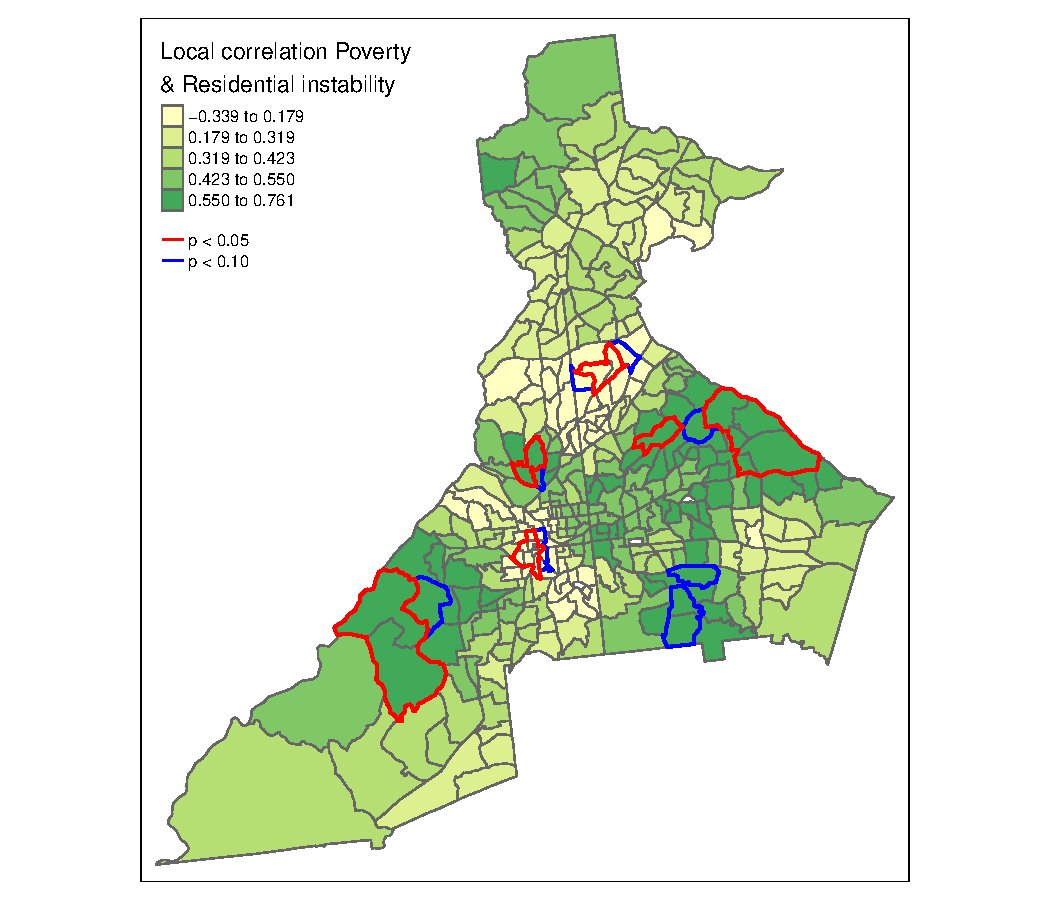
\includegraphics{EPI563-SpatialEPI_files/figure-latex/unnamed-chunk-55-1.pdf}

The Census boundaries include information for all U.S. counties \emph{and territories}! Therefore the map looks this way because Guam, American Samoa, Puerto Rico, as well as Hawaii and Alaska are included. If you were only interested in mapping the "*lower 48" or contiguous states, you could exclude these. In the code below, I also transform or project the data to Albers Equal Area using EPSG code

\begin{lstlisting}[language=R]
us <- us %>%
  filter(!(STATEFP %in% c('02', '15', '66', '60', '78', '72', '69'))) %>%
  select(GEOID, STATEFP, COUNTYFP, NAME) %>%
  st_transform(5070)

plot(st_geometry(us))
\end{lstlisting}

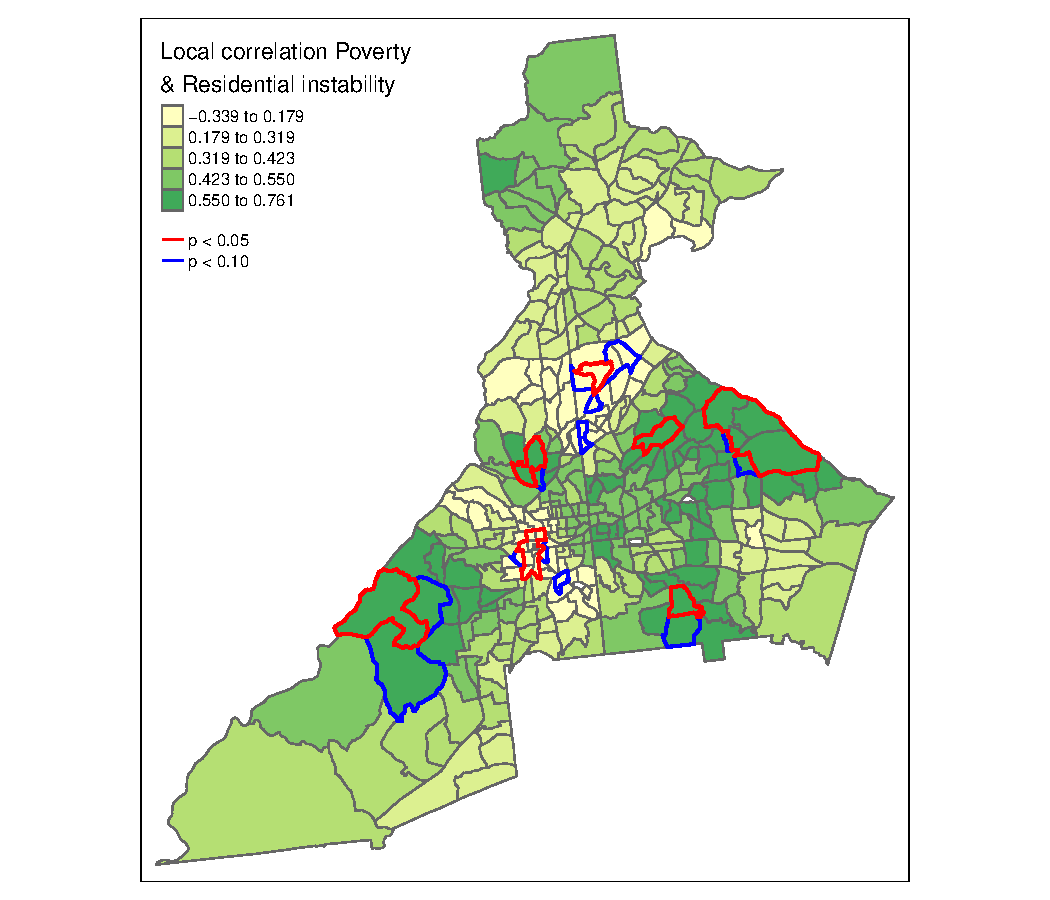
\includegraphics{EPI563-SpatialEPI_files/figure-latex/unnamed-chunk-56-1.pdf}

\hypertarget{merging-attributes-and-geography}{%
\subsection{Merging Attributes and Geography}\label{merging-attributes-and-geography}}

A final step in data preparation is bringing together the attribute data and the geometry data, assuming it has not already been incorporated. Assuming the attributes are a \passthrough{\lstinline!data.frame!} (or perhaps a \passthrough{\lstinline!tibble!}, which is a \passthrough{\lstinline!tidyverse!} data table object), and the geometry is a \passthrough{\lstinline!sf!} object (which also has class \passthrough{\lstinline!data.frame!}), the merge is straightforward. Here is what is needed for merging or joining data:

\begin{itemize}
\tightlist
\item
  Unique key or ID variable in the attribute data \emph{that matches with the ID in the geometry data}
\item
  Unique key or ID variable in the geometry data \emph{that matches with the ID in the attribute data}
\item
  Matching ID's \textbf{does not require same variable name} but \textbf{does require same variable type}.
\end{itemize}

If you are merging several datasets, and one of them is an \passthrough{\lstinline!sf!} object, put that dataset first in the sequence, as that will insure that the final object remains of class \passthrough{\lstinline!sf!}. If you cannot put the \passthrough{\lstinline!sf!} first, you may need to \emph{re-define} the object as \passthrough{\lstinline!sf!} at the end. \protect\hyperlink{st-as-sf}{See the Appendix on \passthrough{\lstinline!st\_as\_sf()!} for more detail}.

\begin{lstlisting}[language=R]
us2 <- us %>%
  left_join(death, by = c('GEOID' = 'FIPS')) %>%
  left_join(uninsured, by = 'GEOID')
\end{lstlisting}

\hypertarget{mapping-mortality-uninsured}{%
\subsection{Mapping Mortality \& Uninsured}\label{mapping-mortality-uninsured}}

\begin{lstlisting}[language=R]
library(tmap)

t1 <- tm_shape(us2) + 
  tm_fill('crude',
          style = 'quantile',
          palette = 'BuPu',
          title = 'Rate per 100,000 py') + 
  tm_borders(alpha = 0.2) +
tm_credits('Source: CDC Wonder',
           position = c('RIGHT', 'BOTTOM')) + 
tm_layout(main.title = 'All-cause mortality rate, 2016-2018',
          bg.color = 'grey85')

t2 <- tm_shape(us2) + 
  tm_fill('uninsured',
          style = 'quantile',
          palette = 'YlOrRd',
          title = '% Uninsured',
          legend.format = list(fun=function(x) paste0(formatC(x * 100, 
                                                              digits=1, 
                                                              format="f"), "%"))) +
  tm_borders(alpha = 0.2) +
tm_credits('Source: American Community Survey',
           position = c('RIGHT', 'BOTTOM')) + 
tm_layout(main.title = 'Uninsured Prevalence, 2014-2018',
          bg.color = 'grey85')


tmap_arrange(t1, t2, ncol = 1)
\end{lstlisting}

\includegraphics{EPI563-SpatialEPI_files/figure-latex/unnamed-chunk-58-1.pdf}

\hypertarget{cartography-for-epidemiology-ii}{%
\chapter{Cartography for Epidemiology II}\label{cartography-for-epidemiology-ii}}

\hypertarget{learning-objectives-w3}{%
\section{Learning objectives, w3}\label{learning-objectives-w3}}

 
  \providecommand{\huxb}[2]{\arrayrulecolor[RGB]{#1}\global\arrayrulewidth=#2pt}
  \providecommand{\huxvb}[2]{\color[RGB]{#1}\vrule width #2pt}
  \providecommand{\huxtpad}[1]{\rule{0pt}{#1}}
  \providecommand{\huxbpad}[1]{\rule[-#1]{0pt}{#1}}

\begin{table}[ht]
\begin{centerbox}
\begin{threeparttable}
\captionsetup{justification=centering,singlelinecheck=off}
\caption{\label{tab:learning-ob} Learning objectives by weekly module}
 \setlength{\tabcolsep}{0pt}
\begin{tabularx}{1\textwidth}{p{1\textwidth}}


\hhline{>{\huxb{255, 255, 255}{1}}-}
\arrayrulecolor{black}

\multicolumn{1}{!{\huxvb{255, 255, 255}{1}}p{1\textwidth}!{\huxvb{255, 255, 255}{1}}}{\cellcolor[RGB]{208, 211, 212}\hspace{6pt}\parbox[b]{1\textwidth-6pt-6pt}{\huxtpad{2pt + 1em}\raggedright \textbf{After this module you should be able to…}\huxbpad{2pt}}} \tabularnewline[-0.5pt]


\hhline{>{\huxb{255, 255, 255}{1}}-}
\arrayrulecolor{black}

\multicolumn{1}{!{\huxvb{255, 255, 255}{1}}p{1\textwidth}!{\huxvb{255, 255, 255}{1}}}{\cellcolor[RGB]{250, 229, 211}\hspace{6pt}\parbox[b]{1\textwidth-6pt-6pt}{\huxtpad{2pt + 1em}\raggedright Describe potential threats to privacy and research ethics that arise when population health data is represented geographically\huxbpad{2pt}}} \tabularnewline[-0.5pt]


\hhline{>{\huxb{255, 255, 255}{1}}-}
\arrayrulecolor{black}

\multicolumn{1}{!{\huxvb{255, 255, 255}{1}}p{1\textwidth}!{\huxvb{255, 255, 255}{1}}}{\cellcolor[RGB]{245, 203, 167}\hspace{6pt}\parbox[b]{1\textwidth-6pt-6pt}{\huxtpad{2pt + 1em}\raggedright Critique spatial epidemiologic literature based on consistency with ethical principles of privacy, avoidance of harm through stigmatization, and balance of benefit and risk\huxbpad{2pt}}} \tabularnewline[-0.5pt]


\hhline{>{\huxb{255, 255, 255}{1}}-}
\arrayrulecolor{black}
\end{tabularx}
\end{threeparttable}\par\end{centerbox}

\end{table}
 

\hypertarget{additional-resources-w3}{%
\section{Additional resources, w3}\label{additional-resources-w3}}

\begin{itemize}
\tightlist
\item
  \href{http://www.ciesin.columbia.edu/pdf/SEDAC_ConfidentialityReport.pdf}{Report on confidentiality issues and policies related to geospatial data for public health applicatins}
\end{itemize}

\hypertarget{important-vocabulary-w3}{%
\section{Important Vocabulary, w3}\label{important-vocabulary-w3}}

 
  \providecommand{\huxb}[2]{\arrayrulecolor[RGB]{#1}\global\arrayrulewidth=#2pt}
  \providecommand{\huxvb}[2]{\color[RGB]{#1}\vrule width #2pt}
  \providecommand{\huxtpad}[1]{\rule{0pt}{#1}}
  \providecommand{\huxbpad}[1]{\rule[-#1]{0pt}{#1}}

\begin{table}[ht]
\begin{centerbox}
\begin{threeparttable}
\captionsetup{justification=centering,singlelinecheck=off}
\caption{\label{tab:unnamed-chunk-61} Vocabulary for Week 3}
 \setlength{\tabcolsep}{0pt}
\begin{tabularx}{0.9\textwidth}{p{0.45\textwidth} p{0.45\textwidth}}


\hhline{>{\huxb{255, 255, 255}{1}}->{\huxb{255, 255, 255}{1}}-}
\arrayrulecolor{black}

\multicolumn{1}{!{\huxvb{255, 255, 255}{1}}p{0.45\textwidth}!{\huxvb{255, 255, 255}{1}}}{\cellcolor[RGB]{84, 153, 199}\hspace{6pt}\parbox[b]{0.45\textwidth-6pt-2pt}{\huxtpad{2pt + 1em}\raggedright \textbf{\textcolor[RGB]{255, 255, 255}{Term}}\huxbpad{2pt}}} &
\multicolumn{1}{p{0.45\textwidth}!{\huxvb{255, 255, 255}{1}}}{\cellcolor[RGB]{84, 153, 199}\hspace{2pt}\parbox[b]{0.45\textwidth-2pt-6pt}{\huxtpad{2pt + 1em}\raggedright \textbf{\textcolor[RGB]{255, 255, 255}{Definition}}\huxbpad{2pt}}} \tabularnewline[-0.5pt]


\hhline{>{\huxb{255, 255, 255}{1}}->{\huxb{255, 255, 255}{1}}-}
\arrayrulecolor{black}

\multicolumn{1}{!{\huxvb{255, 255, 255}{1}}p{0.45\textwidth}!{\huxvb{255, 255, 255}{1}}}{\cellcolor[RGB]{212, 230, 241}\hspace{6pt}\parbox[b]{0.45\textwidth-6pt-2pt}{\huxtpad{2pt + 1em}\raggedright \textbf{Confidentiality}\huxbpad{2pt}}} &
\multicolumn{1}{p{0.45\textwidth}!{\huxvb{255, 255, 255}{1}}}{\cellcolor[RGB]{212, 230, 241}\hspace{2pt}\parbox[b]{0.45\textwidth-2pt-6pt}{\huxtpad{2pt + 1em}\raggedright The duty of anyone entrusted with health information to keep that information private\huxbpad{2pt}}} \tabularnewline[-0.5pt]


\hhline{>{\huxb{255, 255, 255}{1}}->{\huxb{255, 255, 255}{1}}-}
\arrayrulecolor{black}

\multicolumn{1}{!{\huxvb{255, 255, 255}{1}}p{0.45\textwidth}!{\huxvb{255, 255, 255}{1}}}{\cellcolor[RGB]{169, 204, 227}\hspace{6pt}\parbox[b]{0.45\textwidth-6pt-2pt}{\huxtpad{2pt + 1em}\raggedright \textbf{Ethical principles: beneficence}\huxbpad{2pt}}} &
\multicolumn{1}{p{0.45\textwidth}!{\huxvb{255, 255, 255}{1}}}{\cellcolor[RGB]{169, 204, 227}\hspace{2pt}\parbox[b]{0.45\textwidth-2pt-6pt}{\huxtpad{2pt + 1em}\raggedright Two general rules have been formulated as complementary expressions of beneficent actions in this sense: (1) do not harm (e.g. non-maleficence) and (2) maximize possible benefits and minimize possible harms\huxbpad{2pt}}} \tabularnewline[-0.5pt]


\hhline{>{\huxb{255, 255, 255}{1}}->{\huxb{255, 255, 255}{1}}-}
\arrayrulecolor{black}

\multicolumn{1}{!{\huxvb{255, 255, 255}{1}}p{0.45\textwidth}!{\huxvb{255, 255, 255}{1}}}{\cellcolor[RGB]{212, 230, 241}\hspace{6pt}\parbox[b]{0.45\textwidth-6pt-2pt}{\huxtpad{2pt + 1em}\raggedright \textbf{Ethical principles: justice}\huxbpad{2pt}}} &
\multicolumn{1}{p{0.45\textwidth}!{\huxvb{255, 255, 255}{1}}}{\cellcolor[RGB]{212, 230, 241}\hspace{2pt}\parbox[b]{0.45\textwidth-2pt-6pt}{\huxtpad{2pt + 1em}\raggedright Ethical principle that the burdens and benefits of research and public health practice should be justly distributed, including attention to need, effort, contribution, and merit\huxbpad{2pt}}} \tabularnewline[-0.5pt]


\hhline{>{\huxb{255, 255, 255}{1}}->{\huxb{255, 255, 255}{1}}-}
\arrayrulecolor{black}

\multicolumn{1}{!{\huxvb{255, 255, 255}{1}}p{0.45\textwidth}!{\huxvb{255, 255, 255}{1}}}{\cellcolor[RGB]{169, 204, 227}\hspace{6pt}\parbox[b]{0.45\textwidth-6pt-2pt}{\huxtpad{2pt + 1em}\raggedright \textbf{Ethical principles: respect for persons}\huxbpad{2pt}}} &
\multicolumn{1}{p{0.45\textwidth}!{\huxvb{255, 255, 255}{1}}}{\cellcolor[RGB]{169, 204, 227}\hspace{2pt}\parbox[b]{0.45\textwidth-2pt-6pt}{\huxtpad{2pt + 1em}\raggedright Defined by two ethical convictions: a) individuals should be treated as autonomous agents; b) persons with diminished autonomy are entitled to protection\huxbpad{2pt}}} \tabularnewline[-0.5pt]


\hhline{>{\huxb{255, 255, 255}{1}}->{\huxb{255, 255, 255}{1}}-}
\arrayrulecolor{black}

\multicolumn{1}{!{\huxvb{255, 255, 255}{1}}p{0.45\textwidth}!{\huxvb{255, 255, 255}{1}}}{\cellcolor[RGB]{212, 230, 241}\hspace{6pt}\parbox[b]{0.45\textwidth-6pt-2pt}{\huxtpad{2pt + 1em}\raggedright \textbf{Geomask}\huxbpad{2pt}}} &
\multicolumn{1}{p{0.45\textwidth}!{\huxvb{255, 255, 255}{1}}}{\cellcolor[RGB]{212, 230, 241}\hspace{2pt}\parbox[b]{0.45\textwidth-2pt-6pt}{\huxtpad{2pt + 1em}\raggedright A class of methods for changing the geographic location of an individual in an unpredictable way to protect confidentiality, while trying to preserve the relationship between geocoded locations and disease occurrence (Sherman and Fetters 2007, Wiggins 2002)\huxbpad{2pt}}} \tabularnewline[-0.5pt]


\hhline{>{\huxb{255, 255, 255}{1}}->{\huxb{255, 255, 255}{1}}-}
\arrayrulecolor{black}

\multicolumn{1}{!{\huxvb{255, 255, 255}{1}}p{0.45\textwidth}!{\huxvb{255, 255, 255}{1}}}{\cellcolor[RGB]{169, 204, 227}\hspace{6pt}\parbox[b]{0.45\textwidth-6pt-2pt}{\huxtpad{2pt + 1em}\raggedright \textbf{Privacy}\huxbpad{2pt}}} &
\multicolumn{1}{p{0.45\textwidth}!{\huxvb{255, 255, 255}{1}}}{\cellcolor[RGB]{169, 204, 227}\hspace{2pt}\parbox[b]{0.45\textwidth-2pt-6pt}{\huxtpad{2pt + 1em}\raggedright The right of an individual to keep his or her information (health related or otherwise) private\huxbpad{2pt}}} \tabularnewline[-0.5pt]


\hhline{>{\huxb{255, 255, 255}{1}}->{\huxb{255, 255, 255}{1}}-}
\arrayrulecolor{black}
\end{tabularx}
\end{threeparttable}\par\end{centerbox}

\end{table}
 

\hypertarget{spatial-thinking-in-epidemiology-w3}{%
\section{Spatial Thinking in Epidemiology, w3}\label{spatial-thinking-in-epidemiology-w3}}

\begin{quote}
``Progress in achieving health for all depends upon effectively collecting, integrating, and
utilizing medical, public health, socioeconomic, environmental, and physical science data.''
\end{quote}

\begin{quote}
``Although new technological advances can empower individuals and neighborhoods seeking
resources for better health care, they have also heightened concerns about individual privacy
and confidentiality.''
\end{quote}

\begin{quote}
\begin{quote}
\href{http://www.ciesin.columbia.edu/pdf/SEDAC_ConfidentialityReport.pdf}{\emph{-- Confidentiality Issues and Policies Related to the Utilization and Dissemination of Geospatial Data for Public Health Applications}}
\end{quote}
\end{quote}

Ethical concern for justice, beneficence, and respect for persons ground guidelines and practices in responsible conduct of public health research. When we work with geospatial data these concerns are not lessened but instead often are heightened, because of the power of locational information as a means for discerning private information and the risk for intended or unintended breaches of confidentiality and even the transmission of stigma to groups by highlighting health status in marginalized populations.

\hypertarget{risks-of-privacy-breaches-in-collection-of-geospatial-information}{%
\subsection{Risks of privacy breaches in collection of geospatial information}\label{risks-of-privacy-breaches-in-collection-of-geospatial-information}}

Geographic identifiers below the scale of the state (e.g.~county, city, census tract, address) are considered \emph{Protected Health Information } under HIPAA \emph{if they are connected to individual health information}. Surveillance and research activities routinely collect geospatial information for contact or notification purposes, or for reporting, although many consent forms do not explicitly explain the intended purpose or use of the geospatial information.

While any individual should expect protection of privacy not only of individual PHI such as date of birth or name, it is not always explicit that information such as address can be uniquely identifiable and is linkable to other data. Privacy is breached when app-based geocodes are captured without consent, or when geospatial information is collected without express consent (e.g.~if a research respondent is asked to report the address for someone in their social network without that persons consent).

While respect for personal autonomy dictates that individuals should be permitted control of private information, there can also be risks beyond breach of privacy. In some instances, disclosed geospatial information could result in harms to the participant or others. For example collected address information could inadvertently be released to someone seeking to commit violence (e.g as in the case of intimate partner violence). Similarly, studies collecting geospatial information can (and have) been requested by force of law to aid in the investigation or prosecution of suspected crimes. Thus the collection of geospatial information must be well reasoned with respect to risk and benefit to the participant, with appropriate notification and consenting process, and protections in place to maintain confidentiality.

\hypertarget{risk-of-confidentiality-breaches-through-unintentional-de-identification}{%
\subsection{Risk of confidentiality breaches through unintentional de-identification}\label{risk-of-confidentiality-breaches-through-unintentional-de-identification}}

Once private geospatial data has been collected, there is a responsibility for data owners (e.g.~public health agencies, researchers) to protect the confidentiality of that disclosed private information. Confidentiality protection refers to both the secure control of confidential data as well as the avoidance of the unintended re-identification of data deemed `de-identified' through data linkages.

Maintaining data security is critical for all public health research and surveillance activities, but sometimes geospatial data is ignored as a unique identifier. In one instance I submitted a data request to a public health agency to obtain surveillance data on abortion incidence. The data was delivered as an Excel sheet where individual identifiers such as name and date of birth were removed, but the field for address of residence was included. An address is an incredibly powerful unique identifier, particularly when combined with other fields including age or sex.

Geospatial data can be stored separately from other research attributes, maintaining only a key for linkage in the instances when the spatial data are needed. When they are not needed, there is less risk of accidental disclosure of these fields.

Another risk that drives many public health agencies restrictive guidelines around data suppression and reporting, is the concern for re-identification of individuals from aggregated data because of small cell size and the ability to discern identity from quasi-identifiers. For example, age, race, ethnicity, or health outcome could each be quasi-identifiers in some instances when cross-tabulation make individuals unique or nearly so.

In a \href{https://dataprivacylab.org/projects/identifiability/paper1.pdf}{study of the 1990 decennial census}, researchers found that 87\% of the U.S. population could be uniquely identified with only three variables: exact date of birth, zip code, and gender! This is due in part to the combined granularity or specificity of two variables: date of birth and zip code. In most instances, reporting health events at the zip code level without respect to age, or perhaps with age categorized in coarse groups would eliminate the risk. But the take home message is that the stratification of data we prefer for better scientific understanding can quickly lead to at least some sub-groups being individually or nearly individually identifiable.

\hypertarget{risk-of-stigmatization-of-place}{%
\subsection{Risk of stigmatization of place}\label{risk-of-stigmatization-of-place}}

A final ethical concern that is particularly relevant for disease mapping activities is concern for unintentional harm of persons or populations through the stigmatization of place. This can happen when a map identifies locations where marginalized populations spend time, and serves to either further stigmatize that group, or stigmatize others unassociated with the group, but sharing the same location. Such stigmatization can lead to psychosocial harms, but also can alter behavior by other institutional forces including social services, law enforcement, and health services.

Examples of stigmatization of place include the identification of venues where men who have sex with men seek partners, or the mapping of concentrations of commercial sex workers or injection drug users. But the concern for stigmatization of place has also been raised from the point of view of social epidemiology, when predominantly Black and brown neighborhoods are repeatedly characterized as `unhealthy'. The potential harm perpetrated by these maps could arise from the (presumably well-intended) desire to highlight unjust burdens, but the failure to similarly highlight resilience in the face of burdens.

Relatedly, many spatial representations of economic and racial disparities fail to name the factors that give rise to the inequities, including the role of socio-historical and structural discrimination. By failing to name structural racism or policies that serve to concentrate affluence separately from concentrated poverty, the maps contribute to a narrative that the communities are in some way to blame for their health outcomes.

\hypertarget{disease-mapping-i}{%
\chapter{Disease Mapping I}\label{disease-mapping-i}}

\hypertarget{getting-ready-w4}{%
\section{Getting ready, w4}\label{getting-ready-w4}}

\hypertarget{learning-objectives-w4}{%
\subsection{Learning objectives, w4}\label{learning-objectives-w4}}

 
  \providecommand{\huxb}[2]{\arrayrulecolor[RGB]{#1}\global\arrayrulewidth=#2pt}
  \providecommand{\huxvb}[2]{\color[RGB]{#1}\vrule width #2pt}
  \providecommand{\huxtpad}[1]{\rule{0pt}{#1}}
  \providecommand{\huxbpad}[1]{\rule[-#1]{0pt}{#1}}

\begin{table}[ht]
\begin{centerbox}
\begin{threeparttable}
\captionsetup{justification=centering,singlelinecheck=off}
\caption{\label{tab:learning-ob} Learning objectives by weekly module}
 \setlength{\tabcolsep}{0pt}
\begin{tabularx}{1\textwidth}{p{1\textwidth}}


\hhline{>{\huxb{255, 255, 255}{1}}-}
\arrayrulecolor{black}

\multicolumn{1}{!{\huxvb{255, 255, 255}{1}}p{1\textwidth}!{\huxvb{255, 255, 255}{1}}}{\cellcolor[RGB]{208, 211, 212}\hspace{6pt}\parbox[b]{1\textwidth-6pt-6pt}{\huxtpad{2pt + 1em}\raggedright \textbf{After this module you should be able to…}\huxbpad{2pt}}} \tabularnewline[-0.5pt]


\hhline{>{\huxb{255, 255, 255}{1}}-}
\arrayrulecolor{black}

\multicolumn{1}{!{\huxvb{255, 255, 255}{1}}p{1\textwidth}!{\huxvb{255, 255, 255}{1}}}{\cellcolor[RGB]{250, 229, 211}\hspace{6pt}\parbox[b]{1\textwidth-6pt-6pt}{\huxtpad{2pt + 1em}\raggedright Determine and defend appropriate disease mapping strategies consistent with basic epidemiologic concepts (e.g. study design, sampling strategy, measurement error, and systematic bias)\huxbpad{2pt}}} \tabularnewline[-0.5pt]


\hhline{>{\huxb{255, 255, 255}{1}}-}
\arrayrulecolor{black}

\multicolumn{1}{!{\huxvb{255, 255, 255}{1}}p{1\textwidth}!{\huxvb{255, 255, 255}{1}}}{\cellcolor[RGB]{245, 203, 167}\hspace{6pt}\parbox[b]{1\textwidth-6pt-6pt}{\huxtpad{2pt + 1em}\raggedright Create statistically smoothed, age-adjusted disease maps of epidemiologic parameters including SMR, disease risk or rate, and measures of estimate precision/stability\huxbpad{2pt}}} \tabularnewline[-0.5pt]


\hhline{>{\huxb{255, 255, 255}{1}}-}
\arrayrulecolor{black}

\multicolumn{1}{!{\huxvb{255, 255, 255}{1}}p{1\textwidth}!{\huxvb{255, 255, 255}{1}}}{\cellcolor[RGB]{250, 229, 211}\hspace{6pt}\parbox[b]{1\textwidth-6pt-6pt}{\huxtpad{2pt + 1em}\raggedright Describe the modifiable areal unit problem and discuss strategies for evaluating bias arising from MAUP\huxbpad{2pt}}} \tabularnewline[-0.5pt]


\hhline{>{\huxb{255, 255, 255}{1}}-}
\arrayrulecolor{black}
\end{tabularx}
\end{threeparttable}\par\end{centerbox}

\end{table}
 

\hypertarget{additional-resources-w4}{%
\subsection{Additional Resources, w4}\label{additional-resources-w4}}

\begin{itemize}
\tightlist
\item
  \href{https://arriannaplaney.wordpress.com/2018/09/20/brief-notes-on-the-modifiable-areal-unit-problem-maup-in-spatial-analysis-the-case-of-the-zip-code/}{Arianna Planey blog on spatial thinking and MAUP}
\item
  \href{http://emory-primoprod.hosted.exlibrisgroup.com/primo_library/libweb/action/display.do?tabs=detailsTab\&ct=display\&fn=search\&doc=dedupmrg201721517\&indx=1\&recIds=dedupmrg201721517\&recIdxs=0\&elementId=0\&renderMode=poppedOut\&displayMode=full\&frbrVersion=\&frbg=\&\&dscnt=0\&scp.scps=scope\%3A\%28repo\%29\%2Cscope\%3A\%2801EMORY_ALMA\%29\%2CEmory_PrimoThirdNode\&tb=t\&vid=discovere\&mode=Basic\&srt=rank\&vl(274195192UI1)=all_items\&tab=emory_catalog\&dum=true\&vl(freeText0)=waller\%20spatial\%20statistics\&dstmp=1599068943521}{Waller L, Gotway C. Applied Spatial Statistics for Public Health Data. Hoboken, NJ: John Wiley \& Sons, Inc; 2004.}
\item
  \href{https://www-jstor-org.proxy.library.emory.edu/stable/pdf/2532003.pdf}{Clayton D, Kaldor J. Empirical Bayes estimates of age-standardized relative risks for use in disease mapping. Biometrics. 1987 Sep;43(3):671--81.}
\end{itemize}

\hypertarget{important-vocabulary-w4}{%
\subsection{Important Vocabulary, w4}\label{important-vocabulary-w4}}

 
  \providecommand{\huxb}[2]{\arrayrulecolor[RGB]{#1}\global\arrayrulewidth=#2pt}
  \providecommand{\huxvb}[2]{\color[RGB]{#1}\vrule width #2pt}
  \providecommand{\huxtpad}[1]{\rule{0pt}{#1}}
  \providecommand{\huxbpad}[1]{\rule[-#1]{0pt}{#1}}

\begin{table}[ht]
\begin{centerbox}
\begin{threeparttable}
\captionsetup{justification=centering,singlelinecheck=off}
\caption{\label{tab:unnamed-chunk-64} Vocabulary for Week 4}
 \setlength{\tabcolsep}{0pt}
\begin{tabularx}{0.9\textwidth}{p{0.45\textwidth} p{0.45\textwidth}}


\hhline{>{\huxb{255, 255, 255}{1}}->{\huxb{255, 255, 255}{1}}-}
\arrayrulecolor{black}

\multicolumn{1}{!{\huxvb{255, 255, 255}{1}}p{0.45\textwidth}!{\huxvb{255, 255, 255}{1}}}{\cellcolor[RGB]{84, 153, 199}\hspace{6pt}\parbox[b]{0.45\textwidth-6pt-2pt}{\huxtpad{2pt + 1em}\raggedright \textbf{\textcolor[RGB]{255, 255, 255}{Term}}\huxbpad{2pt}}} &
\multicolumn{1}{p{0.45\textwidth}!{\huxvb{255, 255, 255}{1}}}{\cellcolor[RGB]{84, 153, 199}\hspace{2pt}\parbox[b]{0.45\textwidth-2pt-6pt}{\huxtpad{2pt + 1em}\raggedright \textbf{\textcolor[RGB]{255, 255, 255}{Definition}}\huxbpad{2pt}}} \tabularnewline[-0.5pt]


\hhline{>{\huxb{255, 255, 255}{1}}->{\huxb{255, 255, 255}{1}}-}
\arrayrulecolor{black}

\multicolumn{1}{!{\huxvb{255, 255, 255}{1}}p{0.45\textwidth}!{\huxvb{255, 255, 255}{1}}}{\cellcolor[RGB]{212, 230, 241}\hspace{6pt}\parbox[b]{0.45\textwidth-6pt-2pt}{\huxtpad{2pt + 1em}\raggedright \textbf{Bayesian methods}\huxbpad{2pt}}} &
\multicolumn{1}{p{0.45\textwidth}!{\huxvb{255, 255, 255}{1}}}{\cellcolor[RGB]{212, 230, 241}\hspace{2pt}\parbox[b]{0.45\textwidth-2pt-6pt}{\huxtpad{2pt + 1em}\raggedright Methods of statistical inference in which Bayes' theorem is used to update the probability for a hypothesis as more evidence or information becomes available. In disease mapping, the Bayesian framework is frequently used to accomplish rate stabilization and smoothing by using global or local data to inform the 'prior'\huxbpad{2pt}}} \tabularnewline[-0.5pt]


\hhline{>{\huxb{255, 255, 255}{1}}->{\huxb{255, 255, 255}{1}}-}
\arrayrulecolor{black}

\multicolumn{1}{!{\huxvb{255, 255, 255}{1}}p{0.45\textwidth}!{\huxvb{255, 255, 255}{1}}}{\cellcolor[RGB]{169, 204, 227}\hspace{6pt}\parbox[b]{0.45\textwidth-6pt-2pt}{\huxtpad{2pt + 1em}\raggedright \textbf{Empirical Bayes methods}\huxbpad{2pt}}} &
\multicolumn{1}{p{0.45\textwidth}!{\huxvb{255, 255, 255}{1}}}{\cellcolor[RGB]{169, 204, 227}\hspace{2pt}\parbox[b]{0.45\textwidth-2pt-6pt}{\huxtpad{2pt + 1em}\raggedright Estimation procedures in a Bayesian framework in which the prior distribution is estimated from the data. In disease mapping, Empirical Bayes estimators use global or local disease information as a prior in estimating (and smoothing/stabilizing) each local rate\huxbpad{2pt}}} \tabularnewline[-0.5pt]


\hhline{>{\huxb{255, 255, 255}{1}}->{\huxb{255, 255, 255}{1}}-}
\arrayrulecolor{black}

\multicolumn{1}{!{\huxvb{255, 255, 255}{1}}p{0.45\textwidth}!{\huxvb{255, 255, 255}{1}}}{\cellcolor[RGB]{212, 230, 241}\hspace{6pt}\parbox[b]{0.45\textwidth-6pt-2pt}{\huxtpad{2pt + 1em}\raggedright \textbf{Global vs Local spatial analysis}\huxbpad{2pt}}} &
\multicolumn{1}{p{0.45\textwidth}!{\huxvb{255, 255, 255}{1}}}{\cellcolor[RGB]{212, 230, 241}\hspace{2pt}\parbox[b]{0.45\textwidth-2pt-6pt}{\huxtpad{2pt + 1em}\raggedright Global analysis evaluates a pattern or trends that characterizes the entire study region; in contrast local analysis characterizes patterns that are unique to each sub-region of the study area\huxbpad{2pt}}} \tabularnewline[-0.5pt]


\hhline{>{\huxb{255, 255, 255}{1}}->{\huxb{255, 255, 255}{1}}-}
\arrayrulecolor{black}

\multicolumn{1}{!{\huxvb{255, 255, 255}{1}}p{0.45\textwidth}!{\huxvb{255, 255, 255}{1}}}{\cellcolor[RGB]{169, 204, 227}\hspace{6pt}\parbox[b]{0.45\textwidth-6pt-2pt}{\huxtpad{2pt + 1em}\raggedright \textbf{Spatial dependence}\huxbpad{2pt}}} &
\multicolumn{1}{p{0.45\textwidth}!{\huxvb{255, 255, 255}{1}}}{\cellcolor[RGB]{169, 204, 227}\hspace{2pt}\parbox[b]{0.45\textwidth-2pt-6pt}{\huxtpad{2pt + 1em}\raggedright When attribute values or statistical parameters are, on avreage, more similar for nearby places than they are for distant places. Spatial dependence is evaluated by looking at pairs or sets of places.\huxbpad{2pt}}} \tabularnewline[-0.5pt]


\hhline{>{\huxb{255, 255, 255}{1}}->{\huxb{255, 255, 255}{1}}-}
\arrayrulecolor{black}

\multicolumn{1}{!{\huxvb{255, 255, 255}{1}}p{0.45\textwidth}!{\huxvb{255, 255, 255}{1}}}{\cellcolor[RGB]{212, 230, 241}\hspace{6pt}\parbox[b]{0.45\textwidth-6pt-2pt}{\huxtpad{2pt + 1em}\raggedright \textbf{Spatial heterogeneity}\huxbpad{2pt}}} &
\multicolumn{1}{p{0.45\textwidth}!{\huxvb{255, 255, 255}{1}}}{\cellcolor[RGB]{212, 230, 241}\hspace{2pt}\parbox[b]{0.45\textwidth-2pt-6pt}{\huxtpad{2pt + 1em}\raggedright Attributes or statistical parameters are varied (e.g. not homogenous) across sub-areas in a broader region. In Disease mapping we typically are evaluating whether (and how much) disease intensity (risk, rate, prevalence) varies across places.\huxbpad{2pt}}} \tabularnewline[-0.5pt]


\hhline{>{\huxb{255, 255, 255}{1}}->{\huxb{255, 255, 255}{1}}-}
\arrayrulecolor{black}

\multicolumn{1}{!{\huxvb{255, 255, 255}{1}}p{0.45\textwidth}!{\huxvb{255, 255, 255}{1}}}{\cellcolor[RGB]{169, 204, 227}\hspace{6pt}\parbox[b]{0.45\textwidth-6pt-2pt}{\huxtpad{2pt + 1em}\raggedright \textbf{Standardize Morbidity/Mortality Ratio (SMR)}\huxbpad{2pt}}} &
\multicolumn{1}{p{0.45\textwidth}!{\huxvb{255, 255, 255}{1}}}{\cellcolor[RGB]{169, 204, 227}\hspace{2pt}\parbox[b]{0.45\textwidth-2pt-6pt}{\huxtpad{2pt + 1em}\raggedright The ratio of observed to expected disease morbidity or mortality. Often the 'expected' is defined as the overall population (or study-specific) rate; in that case the SMR indicates the relative deviation of a specific unit from the global or overall rate\huxbpad{2pt}}} \tabularnewline[-0.5pt]


\hhline{>{\huxb{255, 255, 255}{1}}->{\huxb{255, 255, 255}{1}}-}
\arrayrulecolor{black}

\multicolumn{1}{!{\huxvb{255, 255, 255}{1}}p{0.45\textwidth}!{\huxvb{255, 255, 255}{1}}}{\cellcolor[RGB]{212, 230, 241}\hspace{6pt}\parbox[b]{0.45\textwidth-6pt-2pt}{\huxtpad{2pt + 1em}\raggedright \textbf{Stationarity vs non-stationarity}\huxbpad{2pt}}} &
\multicolumn{1}{p{0.45\textwidth}!{\huxvb{255, 255, 255}{1}}}{\cellcolor[RGB]{212, 230, 241}\hspace{2pt}\parbox[b]{0.45\textwidth-2pt-6pt}{\huxtpad{2pt + 1em}\raggedright Many statistics assume that the parameter, estimate, or property is constant across sub-units. For example if we take the average height of a population, under stationarity we would assume that average applies equally to sub-populations. In contrast, non-stationarity implies the parameter, estimate, or property varies across sub-groups. In spatial analysis stationarity is an assumption of homogeneity, and non-stationarity allows for heterogeneity.\huxbpad{2pt}}} \tabularnewline[-0.5pt]


\hhline{>{\huxb{255, 255, 255}{1}}->{\huxb{255, 255, 255}{1}}-}
\arrayrulecolor{black}
\end{tabularx}
\end{threeparttable}\par\end{centerbox}

\end{table}
 

\hypertarget{spatial-thinking-in-epidemiology-w4}{%
\section{Spatial Thinking in Epidemiology, w4}\label{spatial-thinking-in-epidemiology-w4}}

\emph{Disease mapping} is located at the intersection of statistics, geography, and epidemiology. Whereas the out-of-the-box GIS approach to making maps of health statistics (e.g.~what I've been referring to as \emph{epidemiologic cartography}) takes raw data and simply shows it on a map, disease mapping typically implies that we are interested in going beyond just making pretty maps. Instead we are driven by core \emph{epidemiologic questions} and concerned about fundamental \emph{epidemiologic and statistical issues}.

\hypertarget{why-do-we-need-disease-mapping}{%
\subsection{Why do we need disease mapping?}\label{why-do-we-need-disease-mapping}}

The defining driver or purpose of epidemiology is an interest in characterizing and estimating the distribution and determinants of health in populations. Disease mapping is primarily focused on the former (distribution of health), providing novel insight into the geographic patterns of health and disease. The latter (determinants of health) can begin to be addressed by Modules 3 and 4 of this course focusing on Clustering and Spatial Regression.

To \emph{spatially describe} the distribution of disease, epidemiologists are primarily interested in one over-arching question:

\begin{quote}
\textbf{Is the intensity of disease or health spatially heterogeneous or spatially homogenous?}
\end{quote}

\emph{Spatial heterogeneity} simply implies that the \emph{global parameter} (e.g.~rate, risk, prevalence, etc) for an entire study area is not identical to the \emph{local parameter} in every sub-region of that study area. In contrast, \emph{spatial homogeneity} means that if you know the overall, global parameter, you basically know every local parameter, plus or minus random variation. Looking for heterogeneity is the whole reason for mapping. If the occurrence of disease were the same everywhere, a map would not tell us much! In previous weeks we mapped disease, but our epidemiologic cartography efforts to date fall short because we did not attend to the following three challenges:

\begin{enumerate}
\def\labelenumi{\arabic{enumi}.}
\tightlist
\item
  Parameter estimate instability due to sparse data/rare events;
\item
  Spurious heterogeneity arising from `\emph{confounding}' by nuisance covariates;
\item
  Biased description of spatial heterogeneity arising from the modifiable areal unit problem (MAUP), a form of the ecologic fallacy
\end{enumerate}

\hypertarget{the-problem-and-approach-to-data-sparsity}{%
\subsubsection{The problem and approach to data sparsity}\label{the-problem-and-approach-to-data-sparsity}}

Reliable and precise estimation of any parameter presumes we have sufficient data to produce a summary (e.g.~a measure of central tendency like a mean, prevalence, risk, etc). When either a disease is quite rare -- resulting in a small numerator -- or the population at risk is quite sparse -- resulting in a small denominator -- the estimate of disease burden is inherently unstable. That means that adding just one or two more events or persons at risk has a notable impact on the estimate. For instance imagine a county with 10 people. In one year, perhaps none die, in the next year one dies, and in the third year three die. The mortality rate is estimated at 0\%, 10\% and 30\%, when none of those seems very plausible as an average expected mortality. The problem is the estimate of mortality rate is derived from too little data.

In practice, public health agencies often suppress data when counts are small, both out of concern for confidentiality, but also because the resulting estimates are so unstable as to be potentially misleading. We have already discussed two approaches to address data sparsity and the resulting parameter \emph{instability} or \emph{imprecision}:

\begin{itemize}
\tightlist
\item
  Aggregate over more time to increase the opportunity for events, or extend the amount of person-time
\item
  Aggregate over geographic units to pool together larger populations. For example data for mortality may be too sparse at the census tract level but might be stable after pooling all tracts to their respective county level.
\end{itemize}

We will spend the next several weeks exploring a range of methods that together constitute a third option: \emph{statistical smoothing or stabilization}. These tools use the amount of information (as a function of sample size) to smooth extreme highs and extreme lows in an effort to recover a plausible `\emph{true}' amount of spatial heterogeneity. A critical goal of disease rate stabilization is that we do not smooth any more than is necessary, so that \emph{true highs and lows} persist, but \emph{spurious or unstable} values are adjusted.

This week we will use aspatial or global \emph{Empirical Bayes} estimators as our first approach to parameter stabilization. In future weeks we will explore \emph{spatial Empirical Bayes}, \emph{kernel density estimators}, and \emph{fully Bayesian estimators} as additional strategies for producing maps that highlights the \emph{signal of spatial heterogeneity} net of the \emph{noise from random error}.

\hypertarget{the-problem-and-approach-to-confounding}{%
\subsubsection{The problem and approach to confounding}\label{the-problem-and-approach-to-confounding}}

Confounding in epidemiology refers to a specific causal structure, wherein the association between a putative exposure and a target disease outcome is spuriously biased because of a backdoor path through one or more confounders. In disease mapping we do not have a formal `\emph{exposure}', with \emph{place} perhaps being a stand-in for unmeasured attributes that vary through space. Therefore we probably should not call this \emph{confounding} in the strictest sense of the word.

Instead you can imagine that there are covariates that are simply a \emph{nuisance}. That means they explain some amount of spatial heterogeneity, but you as the epidemiologist are not particularly interested in their role as an explanation; instead you wish to know if there is still heterogeneity above and beyond those covariates. For example consider comparison of mortality rates by state:

\begin{longtable}[]{@{}lll@{}}
\toprule
\begin{minipage}[b]{0.10\columnwidth}\raggedright
State\strut
\end{minipage} & \begin{minipage}[b]{0.41\columnwidth}\raggedright
Crude mortality rate (per 100,000)\strut
\end{minipage} & \begin{minipage}[b]{0.41\columnwidth}\raggedright
Age-adjusted mortality rate (per 100,000)\strut
\end{minipage}\tabularnewline
\midrule
\endhead
\begin{minipage}[t]{0.10\columnwidth}\raggedright
Florida\strut
\end{minipage} & \begin{minipage}[t]{0.41\columnwidth}\raggedright
957.3\strut
\end{minipage} & \begin{minipage}[t]{0.41\columnwidth}\raggedright
666.6\strut
\end{minipage}\tabularnewline
\begin{minipage}[t]{0.10\columnwidth}\raggedright
Alaska\strut
\end{minipage} & \begin{minipage}[t]{0.41\columnwidth}\raggedright
605.7\strut
\end{minipage} & \begin{minipage}[t]{0.41\columnwidth}\raggedright
745.6\strut
\end{minipage}\tabularnewline
\bottomrule
\end{longtable}

Using the crude mortality rate, it is clear that Florida has a mortality rate perhaps 30\% higher than Alaska, suggesting something really awful is going on in Florida! However once we adjust or standardize by age, it is actually Alaska that has a slightly higher mortality rate. Depending on your purpose both numbers are useful, but if mapping mortality across states, you might think that differences in age-structure (e.g.~many more retirees in Florida than Alaska) is a nuisance to accomplishing the goal; so for disease mapping an age-adjusted estimate may be more useful.

The strategies in spatial epidemiology for addressing confounding (e.g.~removing the effects of nuisance variables) is similar to those in non-spatial epidemiology. Standardization, stratification, and regression control are conventional tools. In disease mapping it is quite common to use standardization as a tool to balance or condition on one or more covariates, such as age. However there are methods including the fully Bayesian models and later spatial regression models, where it is possible to control for multiple covariates.

\hypertarget{the-problem-and-approach-to-maup}{%
\subsubsection{The problem and approach to MAUP}\label{the-problem-and-approach-to-maup}}

\href{https://theconversation.com/how-zip-codes-nearly-masked-the-lead-problem-in-flint-65626}{In this interesting article} about the Flint water-lead crisis, a geographer, Richard Sadler, describes mapping some lead-level data from Flint early in the process. There had been some alarms raised about high levels of lead in Flint, but state-based reporting did not identify or detect anomalies. As the geographer points out, this was likely because state-based reporting was based on (aggregated to) zip codes. While zip codes are not ideal geographic units for any disease mapping, it may not be apparent exactly why zip codes could have led public health officials astray in Flint. Until you look at the map of zip code boundaries overlaid city boundaries.

\begin{figure}
\centering
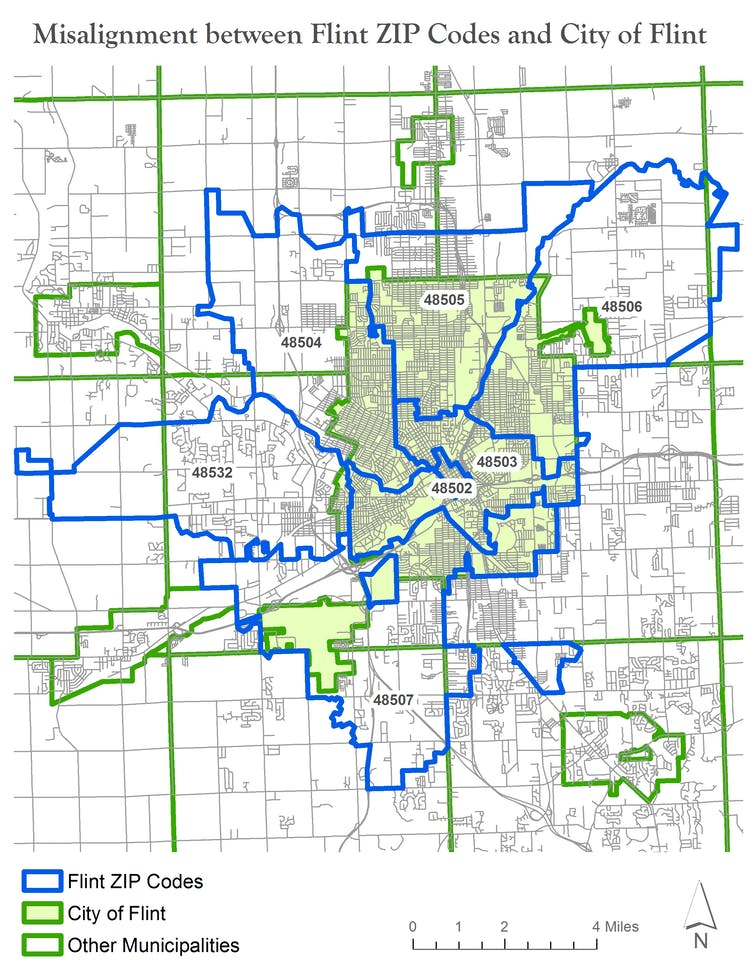
\includegraphics{images/flint-maup.jpg}
\caption{\label{fig:unnamed-chunk-65}Zip code boundaries in Flint, Michigan}
\end{figure}

As you can see, there are seven zip codes in the Flint area, but only two of them are fully contained within the city limits. The others seem evenly split between areas \emph{inside the city limits} and \emph{outside the city}. This became important because the water system issues that produced excess lead exposure \emph{were constrained to households inside the city limits}. The net result was that aggregation of events (high blood lead levels) and population at risk within each zip code area contained a mix of truly exposed and unexposed households. The zip code reporting masked or obscured the true elevations, diluting the early warnings of a problem.

This is a powerful example of the concern referred to by geographers as the \emph{modifiable areal unit problem} (MAUP). Epidemiologists may be familiar with a related idea: the ecologic fallacy or ecologic bias. The problem is not inherently about aggregation. Instead the problem arises when the \emph{way data are aggregated} results in a mixing of different types of people, producing a kind of cross-level confounding. In Flint this meant diluting the population with people exposed to clean water, but it could also result from enriching a specific region with people with confounding risk factors, producing a spurious estimate of the true experience of health within the area.

There are two ways that the MAUP can occur:

\begin{enumerate}
\def\labelenumi{\arabic{enumi}.}
\tightlist
\item
  \textbf{Arbitrary zoning} or boundaries to create aggregates. This is the case in Flint, where one (arbitrary) zoning system (zip codes) was applied to a different zoning system (e.g.~municipal city boundaries). The result is a mis-alignment between what is actually happening and the way we count it up.
\item
  \textbf{Arbitrary scale} or level of aggregation. This occurs when we aggregate to a level or scale that is different from the level or scale at which population health is generated. There is no single `\emph{right}' scale. It depends on the process of interest. The `\emph{correct}' scale for understanding the effect of Medicaid expansion under the ACA is likely different from the `\emph{correct}' or best scale for understanding the role of healthy commercial food retailers on obesity.
\end{enumerate}

One key take away from the above discussion is that the \emph{bias} from the MAUP arises when the way we carry out an analysis does not align with the way that health occurs. In other words, not all aggregation or zoning are similarly harmful. The work for the spatial epidemiologist is to consider how aligned (or mis-aligned) the available aggregation is with respect to the hypothetical process. Sometimes it is possible to explore sensitivity of results to choice of scale or zoning but repeating analyses with alternative boundaries or scales.

\hypertarget{using-statistics-and-probability-models-to-improve-disease-mapping}{%
\subsection{Using statistics and probability models to improve disease mapping}\label{using-statistics-and-probability-models-to-improve-disease-mapping}}

In epidemiology, we spend a lot of time trying to disentangle `\emph{noise}' from `\emph{signal}' in collections of data and their relationships. This is evident in our focus on two broad buckets of error: \emph{random error} that comes from chance and is related to sample size; and \emph{systematic error} that comes from structural bias (e.g.~confounding, selection, misclassification/measurement error) that is not driven by sample size and is therefore not fixed by increasing sample size).

To make inference (make meaning or decisions) from data that take account of random error we adopt statistical probability models that describe the role of chance alone in generating values. For instance many statistics operate under assumptions related to Gaussian or normal distributions. We also rely on Poisson and binomial distributions to evaluate variation and differences for count and binary data respectively.

\hypertarget{how-are-statistics-different-in-space}{%
\subsubsection{How are statistics different in space?}\label{how-are-statistics-different-in-space}}

Spatial statistics is a huge field, well broader than what we will cover this week, or this entire semester. However it is worth introducing a few key ideas to motivate the statistics we will be using.

Health events typically occur at the level of the individual, and individuals can be referenced with respect to their location in space. Consider, for example a study region represented by the blue square in the image below. There is a population distributed across the region, occupying any particular \(x,y\) location. In this population defined by geographic bounds, there may be some individuals experiencing a health event. The set of points observed at a point in time represents a specific realization of a \emph{spatial point process}. In other words we can imagine each individual having some random chance of experiencing the event, and the set of events indexed by their location is one realization or version of the random process.

\begin{figure}
\centering
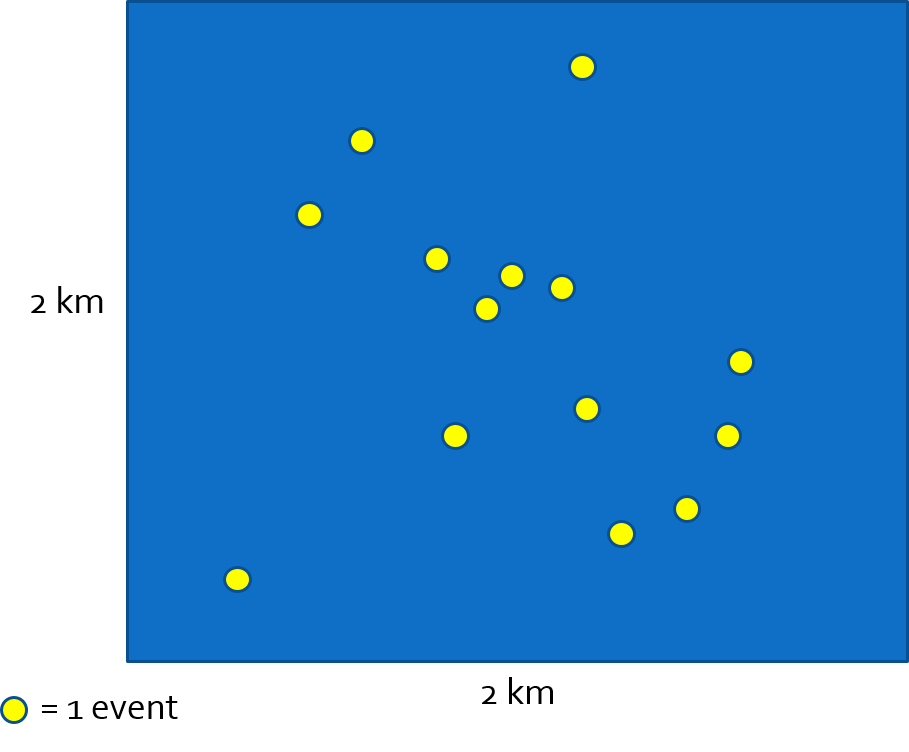
\includegraphics{images/point-process.png}
\caption{\label{fig:unnamed-chunk-66}Spatial point process}
\end{figure}

To describe or quantify what is observed we could describe the \emph{spatial disease intensity} of the event as a spatially continuous surface. In other words for every location, the intensity is the amount of disease per unit-area. To calculate a single, global, measure of spatial intensity for the figure above we divide events by area:

\(\frac{events}{Area}=\frac{14}{4km^{2}}=\frac{3.5}{km^{2}}\)

In this simplistic case we assumed the population at risk was evenly distributed across the study region. More realistically, we can normalize events to the spatially-varying population at risk to quantify the \emph{spatial intensity} of disease.

\begin{figure}
\centering
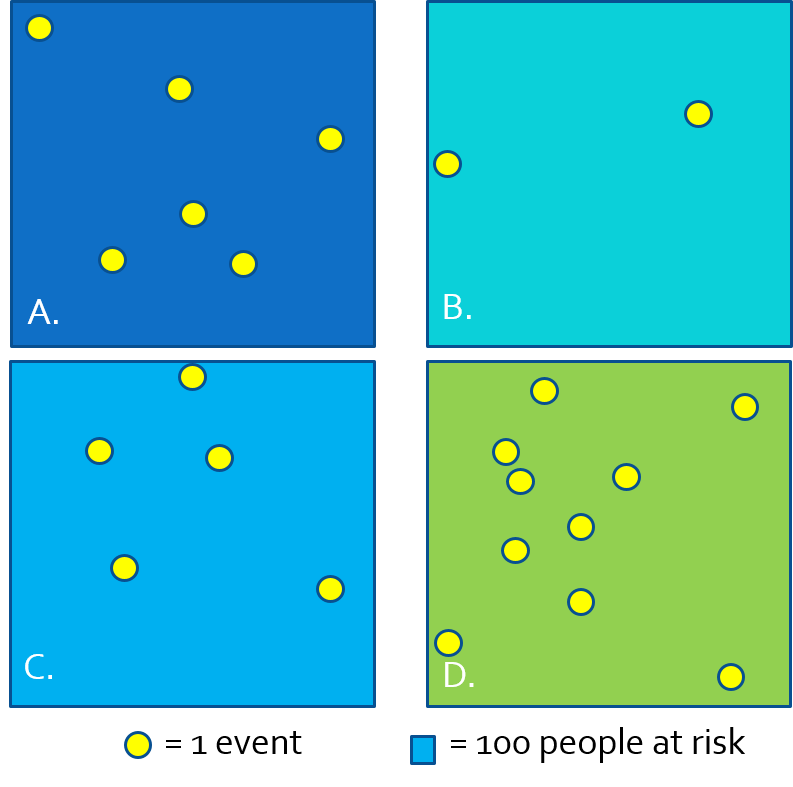
\includegraphics{images/point-process-2.png}
\caption{\label{fig:unnamed-chunk-67}Approximating intensity with areal aggregates}
\end{figure}

Because we often do not have the exact \(x,y\) location of every person at risk and every health event, we cannot observe the full \emph{spatial point process} and thus cannot estimate the continuous \emph{spatial intensity surface}. However, we can approximate the \emph{spatial intensity} by aggregating health events and population and summarizing the ratio (e.g.~as risk, rate, prevalence) per areal unit. In the figure above, each rectangle contains \(n=100\) person-years at risk, producing the following disease rates estimating the spatial intensity of disease:

\begin{longtable}[]{@{}lll@{}}
\toprule
Region & \(\frac{events}{population}\) & Estimate\tabularnewline
\midrule
\endhead
A & \(\frac{6}{100}\) & 6\%\tabularnewline
B & \(\frac{2}{100}\) & 2\%\tabularnewline
C & \(\frac{5}{100}\) & 5\%\tabularnewline
D & \(\frac{10}{100}\) & 10\%\tabularnewline
\bottomrule
\end{longtable}

When we have data in this form (e.g.~counts of events and counts of population), we can use one of several parametric statistical probability distributions common in epidemiology including \emph{Poisson}, \emph{binomial}, and \emph{negative binomial}.

\begin{rmdnote}
\textbf{Why are probability distributions useful?}

Because they provide a model for describing what to expect fro data due to random chance alone. Specifically, relating the count of disease events to a probability distribution permits the calculation of standard errors or confidence intervals expressing the precision or certainty in an estimate. Alternatively we could calculate a \emph{p-value} as a means to test evidence for consistency with a null hypothesis.
\end{rmdnote}

Here is a brief summary of probability distributions common to disease mapping:

\begin{longtable}[]{@{}lll@{}}
\toprule
\begin{minipage}[b]{0.19\columnwidth}\raggedright
Distribution\strut
\end{minipage} & \begin{minipage}[b]{0.31\columnwidth}\raggedright
Paramaterization\strut
\end{minipage} & \begin{minipage}[b]{0.40\columnwidth}\raggedright
MLE and comments\strut
\end{minipage}\tabularnewline
\midrule
\endhead
\begin{minipage}[t]{0.19\columnwidth}\raggedright
Binomial\strut
\end{minipage} & \begin{minipage}[t]{0.31\columnwidth}\raggedright
\(Y_i|r_i\sim Bin(N_i,r_i)\)\strut
\end{minipage} & \begin{minipage}[t]{0.40\columnwidth}\raggedright
\(\hat{r_i}=\frac{Y_i}{N_i}\)\strut
\end{minipage}\tabularnewline
\begin{minipage}[t]{0.19\columnwidth}\raggedright
Poisson\strut
\end{minipage} & \begin{minipage}[t]{0.31\columnwidth}\raggedright
\(Y_i|\theta_i\sim Poisson(E_i\theta_i)\)\strut
\end{minipage} & \begin{minipage}[t]{0.40\columnwidth}\raggedright
\(\theta_i = \frac{Y_i}{E_i}\)\strut
\end{minipage}\tabularnewline
\begin{minipage}[t]{0.19\columnwidth}\raggedright
Poisson-gamma mixture (a.k.a negative binomial)\strut
\end{minipage} & \begin{minipage}[t]{0.31\columnwidth}\raggedright
\(Y_i|\theta_i\sim Poisson(E_i\theta_i)\), \(\theta_i \sim gamma(\alpha, \beta)\)\strut
\end{minipage} & \begin{minipage}[t]{0.40\columnwidth}\raggedright
Note the gamma distribution explains \emph{how much} the \(\theta_i\) varies. In Bayesian framework the gamma is a \emph{prior} for \(\theta\).\strut
\end{minipage}\tabularnewline
\bottomrule
\end{longtable}

In the formulas above:

\begin{itemize}
\tightlist
\item
  \(Y_i\) is the count of health events in the \(i_{th}\) areal unit
\item
  \(N_i\) is the count of population at risk in the \(i_{th}\) areal unit
\item
  \(r_i\) is the risk in the \(i_{th}\) areal unit
\item
  \(E_i\) is the \emph{expected} count, which is calculated as \(N_i\times r\), where \(r\) is an overall reference level of risk. So \emph{expected} simply means the burden of disease in the \(i_{th}\) areal unit if they experienced the reference risk.
\item
  \(\theta_i\) is the \emph{relative risk} in the \(i_{th}\) areal unit; this is essentially the relative deviation of this region from the expected.
\end{itemize}

Don't panic looking at these formulas. Here are some take away points:

\begin{itemize}
\tightlist
\item
  \textbf{Poisson distribution} is a classic distribution to use for evaluating \emph{counts} of events possibly offsetting by the time-at-risk or person-years.

  \begin{itemize}
  \tightlist
  \item
    Poisson assumes that the \emph{mean} of the distribution is the same as the \emph{variance} of the distribution.
  \item
    Poisson distribution only approximates the disease intensity rate well for \emph{rare disease processes}. Therefore Poisson is not a good choice if the outcome is not rare.
  \end{itemize}
\item
  \textbf{Binomial distribution} is useful for characterizing disease occurrence for \emph{non-rare} or common disease processes.
\item
  \textbf{Poisson-gamma Mixture} may be the most foreign. However, you may have heard of the Negative Binomial distribution for count data? Poisson-gamma mixture is essentially a negative binomial model. It is a probability distribution like the Poisson, except without the expectation that the \emph{mean} is equal to the \emph{variance}. In other words it is robust to what is called \emph{over-dispersion}, when the variation in the count is greater than expected under the Poisson.

  \begin{itemize}
  \tightlist
  \item
    Over-dispersion is quite common in spatial epidemiology because there often are unobserved factors driving the occurrence of disease in each area, and those unobserved differences produce event intensity that is not strictly Poisson in nature. We will use Poisson-gamma for this reason.
  \end{itemize}
\end{itemize}

If you want to learn more about \emph{Poisson point processes} or \emph{probability distributions for spatial epidemiology}, I highly recommend Lance Waller's text, \emph{Applied Spatial Statistics for Public Health Data} (Waller \& Gotway, 2004). It is available electronically via Woodruff Library.

\hypertarget{spatial-analysis-in-epidemiology-w4}{%
\section{Spatial Analysis in Epidemiology, w4}\label{spatial-analysis-in-epidemiology-w4}}

As an example dataset, for the next four weeks of disease mapping we will aim to estimate the \emph{spatial heterogeneity} at the county level of the occurrence of \emph{very low birthweight} (VLBW; weight at birth \textless{} 1500 grams) babies in 2018-2019. These data were derived from the \href{https://oasis.state.ga.us/}{Georgia OASIS website}. This outcome is of public health importance because of the high morbidity and mortality associated with being born so early or so small. However, with an overall rate of VLBW of only 1.8\%, it is a rare outcome, and there will likely be sparse data for many rural counties.

\includegraphics{EPI563-SpatialEPI_files/figure-latex/unnamed-chunk-70-1.pdf}

In the maps above, we can visualize the \emph{observed} VLBW prevalence as well as the prevalence restricted only to counties meeting the NCHS suppression rule for natality records (e.g.~suppress reporting of any count \textless{} 10). In the map on the right 85 of the 159 counties of Georgia would have suppressed data. This suggests that, even when we know the values (e.g.~they aren't suppressed) we should be thinking about issues of \emph{imprecision} or \emph{instability} in the estimates (and therefore in the map overall) because so many counties have such sparse data.

\begin{rmdnote}
There are four \textbf{disease mapping objectives} we wish to accomplish to more fully describe these data:

\begin{enumerate}
\def\labelenumi{\arabic{enumi}.}
\tightlist
\item
  Test whether there is statistical evidence for \emph{spatial heterogeneity}
\item
  Describe the precision of VLBW estimates in each county
\item
  Account for possibly spurious patterns due to a confounding covariate
\item
  Produce overall and covariate-adjusted \emph{smoothed} or \emph{stabilized} rate estimates using global Empirical Bayes.
\end{enumerate}
\end{rmdnote}

\hypertarget{disease-mapping-is-there-spatial-heterogeneity}{%
\subsection{Disease mapping: Is there spatial heterogeneity?}\label{disease-mapping-is-there-spatial-heterogeneity}}

\hypertarget{calculating-expected-counts-and-the-smr}{%
\subsubsection{Calculating expected counts and the SMR}\label{calculating-expected-counts-and-the-smr}}

Up until now we have primarily represented disease burden using risks, rates, or prevalence. However, as we introduce statistical estimation under Poisson and Poisson-gamma (negative binomial), we are often testing whether an area deviates \emph{from the expected value}. A natural way to represent this deviation is by using \emph{Standardized Morbidity Ratios} (SMRs) as an alternative to risks or rates:

\(SMR_i=\frac{Y_i}{E_i}\)

The standardized morbidity ratio (could also be standardized \emph{mortality}, \emph{incidence}, or \emph{prevalence} depending on what is being counted) is a measure of \emph{relative excess risk}. It quantifies the deviation of a population parameter (in this case the live birth risk of very low birthweight for a geographically-defined population) from a reference value (in this case the VLBW risk for the whole state of Georgia). The SMR is calculated as the \emph{Observed} count of events, \(Y_i\), over the \emph{Expected} count, \(E_i\), of events.

Calculating \emph{expected} counts of VLBW events in these data is straightforward: first calculate the overall risk, \(r\), and then multiply that by the population at risk in each county, \(N_i\), to get the events expected if there were homogeneity in risk, or if the \(SMR=1.0\) for all counties.

\begin{lstlisting}[language=R]
# the overall ratio of events to population is the global risk
risk <- sum(vlbw$VLBW) / sum(vlbw$TOT) 


# Now add a variable to the dataset representing expected count and SMR
vlbw <- vlbw %>%
  mutate(expect = risk * TOT,
         SMR = VLBW / expect)
\end{lstlisting}

As you can see in the maps below, the SMR represents the same unerlying pattern, but simply does so on a different scale, that of \emph{relative excess risk} rather than \emph{absolute risk}.

\includegraphics{EPI563-SpatialEPI_files/figure-latex/unnamed-chunk-73-1.pdf}

\hypertarget{testing-for-spatial-heterogeneity}{%
\subsubsection{Testing for spatial heterogeneity}\label{testing-for-spatial-heterogeneity}}

Perhaps the fundamental purpose of disease mapping is to describe and represent the magnitude and patterns of \emph{spatial heterogeneity} or variation in health across sub-areas of a study region. But what if there \emph{isn't any real variation}!? For instance consider each of these scenarios:

\begin{itemize}
\tightlist
\item
  There is very little meaningful difference in values, yet we can cartographically represent data as appearing heterogeneous simply by choice of cutpoint and color assignment.
\item
  There appears to be large differences in values between sub-areas, but the counts are so sparse that it is possible all of the seeming difference is due to chance
\end{itemize}

For these reasons it is sensible to start by evaluating the evidence for any versus no heterogeneity. If none, there is little reason to proceed with spatial analysis. Luckily there are standard statistical tests designed just for this purpose: to evaluate whether the count of events is significantly different across observations, accounting for the number of trials or persons at risk.

The \passthrough{\lstinline!R!} package \passthrough{\lstinline!DCluster!} has a function for a \emph{chi-square} test optimized for the needs of aggregated data in spatial epidemiology. The test is called \passthrough{\lstinline!achisq.test()!} and it can evaluate variation in numerator and denominator under a Poisson or Negative Binomial (recall this is same as Poisson-gamma) distribution. The \passthrough{\lstinline!sf!} data object containing the VLBW information is called \passthrough{\lstinline!vlbw!}; within that \passthrough{\lstinline!sf!} object is a column named \passthrough{\lstinline!VLBW!} representing the count of babies born very low birthweight in the county, and another variable named \passthrough{\lstinline!TOT!} representing the count of all live births. In the language of Poisson, \(Y_i\) is the count variable \passthrough{\lstinline!VLBW!} for each county, and we evaluate that count against the \emph{offset} which is the log of the number of births at risk.

Look at the help documentation for this function; here I specify the statistical model as \emph{Poisson}. The argument \passthrough{\lstinline!R=499!} refers to the number of \emph{random permutations} to use in calculating an empirical p-value.

\begin{lstlisting}[language=R]
DCluster::achisq.test(VLBW~offset(log(TOT)), 
                      data = vlbw, 
                      model = 'poisson',
                      R = 499)
\end{lstlisting}

\begin{lstlisting}
## Chi-square test for overdispersion 
## 
## 	Type of boots.: parametric 
## 	Model used when sampling: Poisson 
## 	Number of simulations: 499 
## 	Statistic:  416.6378 
## 	p-value :  0.002
\end{lstlisting}

The null hypothesis is that the \emph{relative risk} or \emph{SMR} is equal to one for all counties. In other words, under the null, there is no meaningful difference in the risk between counties. Based on 499 simulated permutations under the null, the observed data appear \emph{quite inconsistent with the null} assumption, as evidenced by \emph{p.value = 0.002}. In other words under a strictly Poisson probability model, there appears to be significant \emph{spatial heterogeneity} in the risk of VLBW.

\begin{rmdnote}
In conventional statistics we often have \emph{closed form} formulas for calculating standard errors, confidence intervals or p-values. However, in spatial statistics the simple parametric assumptions do not always hold. One empirical alternative to the closed-form formula is to use random permutations of the data to simulate the random data \emph{under the null hypothesis}.

In the case of the \passthrough{\lstinline!achisq.test()!}, the null hypothesis is that the \emph{observed} count is equal to the \emph{expected} count. Random permutations of this would be to take a random Poisson draw for the count in each county under the null. If we repeat that hundreds of times, we have a distribution of what random chance would produce. Then we compare our \emph{actual observed} values to that distribution. If the observed values are \emph{very different from} the set of random values, we might say there is evidence against the null.
\end{rmdnote}

What would happen if we allowed that the distribution under the null was \emph{Negative Binomial} (e.g.~Poisson-Gamma) rather than strictly \emph{Poisson}? We could specify that and re-calculate the \emph{p-value} testing for evidence of significant heterogeneity:

\begin{lstlisting}[language=R]
DCluster::achisq.test(VLBW~offset(log(TOT)), 
                      data = vlbw, 
                      model = 'negbin',
                      R = 499)
\end{lstlisting}

\begin{lstlisting}
## Chi-square test for overdispersion 
## 
## 	Type of boots.: parametric 
## 	Model used when sampling: Negative Binomial 
## 	Number of simulations: 499 
## 	Statistic:  416.6378 
## 	p-value :  0.778
\end{lstlisting}

This assumption seems to give us an entirely different picture of what is going on! While this will not always occur (e.g.~in many instances a test for heterogeneity under either \emph{Poisson} or \emph{Negative Binomial} will result in consistent determination of statistical significance), it is also not a complete surprise. There are two points worth making about the comparison of these two results.

First, to understand how this is possible it might help to visualize the probability distributions themselves to fix in our minds what `\emph{over-dispersion}' or `\emph{extra-Poisson variance}' mean. Here is a plot of 10,000 draws from two random distributions, the \emph{Poisson} and the \emph{Negative Binomial}. In each, the mean expectation under the null is that there are \(10\) events, indicated by the blue dotted line. The left panel is the histogram of how many events occurred (assuming an expected mean of \(n=10\)) with the \emph{Negative Binomial}, and the right panel shows the distribution under random draws from the \emph{Poisson}.

\includegraphics{EPI563-SpatialEPI_files/figure-latex/unnamed-chunk-77-1.pdf}

The \emph{Negative Binomial} distribution is \emph{fatter}, especially in the right-tail. This means that even if the null/expectation of \(n=10\) were true, we would expect a wider range of counts (including more instances of high counts) by chance alone under the \emph{Negative Binomial} as compared with the \emph{Poisson}.

A second point worth making is that this early step -- testing for aspatial heterogeneity -- is just that: a first look. There are many reasons for data to behave with variance in excess of the Poisson expectation. Over-dispersion can arise when there are important missing variables which predict the outcome event and vary spatially. This is quite common. If there were no evidence of spatial heterogeneity under either distribution, we might consider throwing in the towel now. However, given evidence of unusual behavior under a Poisson expectation suggests further exploration might be worthwhile. However, clearly we should consider using the Poisson-Gamma approach for subsequent analyses including Empirical Bayesian smoothing, below.

\hypertarget{disease-mapping-how-precise-are-county-estimates}{%
\subsection{Disease mapping: How precise are county estimates?}\label{disease-mapping-how-precise-are-county-estimates}}

Following the question of whether or not there is global spatial heterogeneity (e.g.~at least some counties have \(SMR\neq 1.0\)), a natural follow up would be how confident or precise are the estimates themselves, and which counties are statistically significantly different from the null expectation?

A function to estimate the continuous \emph{p-value} associated with the SMR is the \passthrough{\lstinline!probmap!} function from the package \passthrough{\lstinline!spdep!}. This function calculates the probabilities (under the Poisson probability model) of observing an event count \emph{more extreme} than what was actually observed, given the expected count (e.g.~we might expect every county had the overall risk). The test is a one-tailed test, and by default the alternative hypothesis is that observed are \emph{less than} expected, or that SMR \textless1.0 (to test for extremes greater than 1.0, set the argument \passthrough{\lstinline!alternative = 'greater'!}).

\begin{rmdnote}
In frequentist statistics we are more familiar with focusing on small \emph{p-values} as evidence to reject the null hypothesis. In the case of the continuous \emph{p-value} returned by \passthrough{\lstinline!probmap!}, we can think about probabilities on either side of the spectrum. For instance, with the default \passthrough{\lstinline!alternative = 'less'!}, a probability that is \(p<0.05\) would indicate an \(SMR<1\) was statistically significant (at \(\alpha=0.05\)). In contrast, \(p>0.95\) would suggest an unusual finding, under the null, for \(SMR>1\). The \(p>0.95\) for the \passthrough{\lstinline!alternative = 'less'!} would therefore be equivalence to the \(p<0.05\) for the \passthrough{\lstinline!alternative = 'greater'!} for describing significance with \(SMR>1\).
\end{rmdnote}

\passthrough{\lstinline!probmap!} expects several arguments including a vector of the count of cases, a vector of the population at risk, and optionally a \passthrough{\lstinline!row.names!} vector to help align observations. Because your job is to identify counties with SMR in excess of expected (e.g.~\textgreater\textgreater1), it is easier to interpret if we change the alternative hypothesis of the one-sided test to be \passthrough{\lstinline!alternative = 'greater'!}.

The function returns the \emph{expected count} (yet another way to get this number!), as well as the SMR (in this case it is named \passthrough{\lstinline!relRisk!}, and somewhat oddly the function multiplies the SMR by 100 so the numbers appear different!), and the Poisson probability that the observed count was more `extreme' than actually observed.

\begin{lstlisting}[language=R]
library(spdep)
x <- probmap(n = vlbw$VLBW, x = vlbw$TOT, 
              row.names = vlbw$GEOID,
             alternative = 'greater')
head(x) # look at what is returned
\end{lstlisting}

 
  \providecommand{\huxb}[2]{\arrayrulecolor[RGB]{#1}\global\arrayrulewidth=#2pt}
  \providecommand{\huxvb}[2]{\color[RGB]{#1}\vrule width #2pt}
  \providecommand{\huxtpad}[1]{\rule{0pt}{#1}}
  \providecommand{\huxbpad}[1]{\rule[-#1]{0pt}{#1}}

\begin{table}[ht]
\begin{centerbox}
\begin{threeparttable}
\captionsetup{justification=centering,singlelinecheck=off}
\caption{\label{tab:unnamed-chunk-79} }
 \setlength{\tabcolsep}{0pt}
\begin{tabular}{l l l l}


\hhline{>{\huxb{0, 0, 0}{0.4}}->{\huxb{0, 0, 0}{0.4}}->{\huxb{0, 0, 0}{0.4}}->{\huxb{0, 0, 0}{0.4}}-}
\arrayrulecolor{black}

\multicolumn{1}{!{\huxvb{0, 0, 0}{0.4}}r!{\huxvb{0, 0, 0}{0}}}{\huxtpad{6pt + 1em}\raggedleft \hspace{6pt} \textbf{raw} \hspace{6pt}\huxbpad{6pt}} &
\multicolumn{1}{r!{\huxvb{0, 0, 0}{0}}}{\huxtpad{6pt + 1em}\raggedleft \hspace{6pt} \textbf{expCount} \hspace{6pt}\huxbpad{6pt}} &
\multicolumn{1}{r!{\huxvb{0, 0, 0}{0}}}{\huxtpad{6pt + 1em}\raggedleft \hspace{6pt} \textbf{relRisk} \hspace{6pt}\huxbpad{6pt}} &
\multicolumn{1}{r!{\huxvb{0, 0, 0}{0.4}}}{\huxtpad{6pt + 1em}\raggedleft \hspace{6pt} \textbf{pmap} \hspace{6pt}\huxbpad{6pt}} \tabularnewline[-0.5pt]


\hhline{>{\huxb{0, 0, 0}{0.4}}->{\huxb{0, 0, 0}{0.4}}->{\huxb{0, 0, 0}{0.4}}->{\huxb{0, 0, 0}{0.4}}-}
\arrayrulecolor{black}

\multicolumn{1}{!{\huxvb{0, 0, 0}{0.4}}r!{\huxvb{0, 0, 0}{0}}}{\cellcolor[RGB]{242, 242, 242}\huxtpad{6pt + 1em}\raggedleft \hspace{6pt} 0.0189 \hspace{6pt}\huxbpad{6pt}} &
\multicolumn{1}{r!{\huxvb{0, 0, 0}{0}}}{\cellcolor[RGB]{242, 242, 242}\huxtpad{6pt + 1em}\raggedleft \hspace{6pt} 424~~~ \hspace{6pt}\huxbpad{6pt}} &
\multicolumn{1}{r!{\huxvb{0, 0, 0}{0}}}{\cellcolor[RGB]{242, 242, 242}\huxtpad{6pt + 1em}\raggedleft \hspace{6pt} 104~~ \hspace{6pt}\huxbpad{6pt}} &
\multicolumn{1}{r!{\huxvb{0, 0, 0}{0.4}}}{\cellcolor[RGB]{242, 242, 242}\huxtpad{6pt + 1em}\raggedleft \hspace{6pt} 0.23~~ \hspace{6pt}\huxbpad{6pt}} \tabularnewline[-0.5pt]


\hhline{>{\huxb{0, 0, 0}{0.4}}|>{\huxb{0, 0, 0}{0.4}}|}
\arrayrulecolor{black}

\multicolumn{1}{!{\huxvb{0, 0, 0}{0.4}}r!{\huxvb{0, 0, 0}{0}}}{\huxtpad{6pt + 1em}\raggedleft \hspace{6pt} 0.0121 \hspace{6pt}\huxbpad{6pt}} &
\multicolumn{1}{r!{\huxvb{0, 0, 0}{0}}}{\huxtpad{6pt + 1em}\raggedleft \hspace{6pt} 19.5~ \hspace{6pt}\huxbpad{6pt}} &
\multicolumn{1}{r!{\huxvb{0, 0, 0}{0}}}{\huxtpad{6pt + 1em}\raggedleft \hspace{6pt} 66.8 \hspace{6pt}\huxbpad{6pt}} &
\multicolumn{1}{r!{\huxvb{0, 0, 0}{0.4}}}{\huxtpad{6pt + 1em}\raggedleft \hspace{6pt} 0.95~~ \hspace{6pt}\huxbpad{6pt}} \tabularnewline[-0.5pt]


\hhline{>{\huxb{0, 0, 0}{0.4}}|>{\huxb{0, 0, 0}{0.4}}|}
\arrayrulecolor{black}

\multicolumn{1}{!{\huxvb{0, 0, 0}{0.4}}r!{\huxvb{0, 0, 0}{0}}}{\cellcolor[RGB]{242, 242, 242}\huxtpad{6pt + 1em}\raggedleft \hspace{6pt} 0.0179 \hspace{6pt}\huxbpad{6pt}} &
\multicolumn{1}{r!{\huxvb{0, 0, 0}{0}}}{\cellcolor[RGB]{242, 242, 242}\huxtpad{6pt + 1em}\raggedleft \hspace{6pt} 414~~~ \hspace{6pt}\huxbpad{6pt}} &
\multicolumn{1}{r!{\huxvb{0, 0, 0}{0}}}{\cellcolor[RGB]{242, 242, 242}\huxtpad{6pt + 1em}\raggedleft \hspace{6pt} 98.5 \hspace{6pt}\huxbpad{6pt}} &
\multicolumn{1}{r!{\huxvb{0, 0, 0}{0.4}}}{\cellcolor[RGB]{242, 242, 242}\huxtpad{6pt + 1em}\raggedleft \hspace{6pt} 0.625~ \hspace{6pt}\huxbpad{6pt}} \tabularnewline[-0.5pt]


\hhline{>{\huxb{0, 0, 0}{0.4}}|>{\huxb{0, 0, 0}{0.4}}|}
\arrayrulecolor{black}

\multicolumn{1}{!{\huxvb{0, 0, 0}{0.4}}r!{\huxvb{0, 0, 0}{0}}}{\huxtpad{6pt + 1em}\raggedleft \hspace{6pt} 0.0242 \hspace{6pt}\huxbpad{6pt}} &
\multicolumn{1}{r!{\huxvb{0, 0, 0}{0}}}{\huxtpad{6pt + 1em}\raggedleft \hspace{6pt} 33.1~ \hspace{6pt}\huxbpad{6pt}} &
\multicolumn{1}{r!{\huxvb{0, 0, 0}{0}}}{\huxtpad{6pt + 1em}\raggedleft \hspace{6pt} 133~~ \hspace{6pt}\huxbpad{6pt}} &
\multicolumn{1}{r!{\huxvb{0, 0, 0}{0.4}}}{\huxtpad{6pt + 1em}\raggedleft \hspace{6pt} 0.0403 \hspace{6pt}\huxbpad{6pt}} \tabularnewline[-0.5pt]


\hhline{>{\huxb{0, 0, 0}{0.4}}|>{\huxb{0, 0, 0}{0.4}}|}
\arrayrulecolor{black}

\multicolumn{1}{!{\huxvb{0, 0, 0}{0.4}}r!{\huxvb{0, 0, 0}{0}}}{\cellcolor[RGB]{242, 242, 242}\huxtpad{6pt + 1em}\raggedleft \hspace{6pt} 0.012~ \hspace{6pt}\huxbpad{6pt}} &
\multicolumn{1}{r!{\huxvb{0, 0, 0}{0}}}{\cellcolor[RGB]{242, 242, 242}\huxtpad{6pt + 1em}\raggedleft \hspace{6pt} 4.53 \hspace{6pt}\huxbpad{6pt}} &
\multicolumn{1}{r!{\huxvb{0, 0, 0}{0}}}{\cellcolor[RGB]{242, 242, 242}\huxtpad{6pt + 1em}\raggedleft \hspace{6pt} 66.2 \hspace{6pt}\huxbpad{6pt}} &
\multicolumn{1}{r!{\huxvb{0, 0, 0}{0.4}}}{\cellcolor[RGB]{242, 242, 242}\huxtpad{6pt + 1em}\raggedleft \hspace{6pt} 0.83~~ \hspace{6pt}\huxbpad{6pt}} \tabularnewline[-0.5pt]


\hhline{>{\huxb{0, 0, 0}{0.4}}|>{\huxb{0, 0, 0}{0.4}}|}
\arrayrulecolor{black}

\multicolumn{1}{!{\huxvb{0, 0, 0}{0.4}}r!{\huxvb{0, 0, 0}{0}}}{\huxtpad{6pt + 1em}\raggedleft \hspace{6pt} 0.0136 \hspace{6pt}\huxbpad{6pt}} &
\multicolumn{1}{r!{\huxvb{0, 0, 0}{0}}}{\huxtpad{6pt + 1em}\raggedleft \hspace{6pt} 13.3~ \hspace{6pt}\huxbpad{6pt}} &
\multicolumn{1}{r!{\huxvb{0, 0, 0}{0}}}{\huxtpad{6pt + 1em}\raggedleft \hspace{6pt} 75~~ \hspace{6pt}\huxbpad{6pt}} &
\multicolumn{1}{r!{\huxvb{0, 0, 0}{0.4}}}{\huxtpad{6pt + 1em}\raggedleft \hspace{6pt} 0.855~ \hspace{6pt}\huxbpad{6pt}} \tabularnewline[-0.5pt]


\hhline{>{\huxb{0, 0, 0}{0.4}}->{\huxb{0, 0, 0}{0.4}}->{\huxb{0, 0, 0}{0.4}}->{\huxb{0, 0, 0}{0.4}}-}
\arrayrulecolor{black}
\end{tabular}
\end{threeparttable}\par\end{centerbox}

\end{table}
 

As you can see, the function calculates:

\begin{itemize}
\tightlist
\item
  \emph{Raw rate}, which is simply \(\frac{Y_i}{N_i}\)
\item
  \emph{Expected count}, which is simply \(r\times N_i\), where \(r\) is the overall expected rate
\item
  \emph{Relative risk}, which is also the SMR and is the ratio of the observed to expected. Note that the function multiplies the SMR by 100. So the value 103 actually refers to an SMR of 1.03
\item
  \emph{p-value}, which again is the probability that the risk in this county was significantly greater than 1.0
\end{itemize}

For mapping, we will grab the SMR (e.g.~\passthrough{\lstinline!relRisk!} but divided by 100 to make it more conventional) and the \emph{p-value} term, \passthrough{\lstinline!pmap!}, which we can easily add to our \passthrough{\lstinline!sf!} object:

\begin{lstlisting}[language=R]
vlbw$pmap <- x$pmap

vlbw$SMR <- x$relRisk / 100
\end{lstlisting}

\hypertarget{mapping-the-p-value-for-the-smr}{%
\subsubsection{Mapping the p-value for the SMR}\label{mapping-the-p-value-for-the-smr}}

To produce a \textbf{p-value map} depicting the continuous probability that we would observe an SMR that is more extreme than observed (and specifically in this case, \emph{greater} than observed), assuming the null described by the expected count is true, we could use the probability retrieved from the previous code in a map, next to the map of the SMR itself:

\begin{lstlisting}[language=R]
smr_map <- tm_shape(vlbw) +
  tm_fill('SMR',
          style = 'fixed', 
          palette = '-RdYlBu',
          breaks = c(0.13, 0.67, 0.9, 1.1, 1.4, 2.3),
          title = 'Std. Morbidity Ratio') + 
  tm_borders() +
  tm_layout(main.title = 'VLBW in Georgia, 2018-2019',
            inner.margins = c(0.02, 0.02,0.05,0.2))+
  tm_shape(ga) +
  tm_borders(lwd = 2, col = 'black')

prob <- tm_shape(vlbw) + 
  tm_fill('pmap',
          style = 'cont',
          palette = 'PiYG',
          n=7,
          title = 'Prob SMR > 1\nby chance alone') + 
  tm_borders() + 
  tm_layout(main.title = 'Probability Map',
            inner.margins = c(0.02, 0.02,0.05,0.2))+
  tm_shape(ga) +
  tm_borders(lwd = 2, col = 'black')

tmap_arrange(smr_map, prob)
\end{lstlisting}

\includegraphics{EPI563-SpatialEPI_files/figure-latex/unnamed-chunk-81-1.pdf}

While this is interesting, perhaps what is more useful would be to quantify these probabilities into familiar thresholds. For example we could use the output of the \passthrough{\lstinline!probmap()!} function to calculate custom p-value categories.

The following code does several things:

\begin{itemize}
\tightlist
\item
  REMEMBER: \passthrough{\lstinline!probmap!} carried out a 1-sided test, but to make this align with results from the confidence intervals where we identified counties with extreme values \emph{in either direction}, which were implicitly two-sided, we will look for counties with p \textgreater{} 0.975.
\item
  By using \passthrough{\lstinline!group\_by(pmap.pv)!} along with \passthrough{\lstinline!summarise()!}, this code \emph{dissolves} any adjacent counties that are significant (or not significant). The result will be a map with general borders around sets of significant counties rather than around each county separately.
\item
  Finally, by using \passthrough{\lstinline!filter(pmap.pv == 1)!} this code removes the counties that are \emph{not significant}. The result is the desired dark borders only for counties that are statistically significantly higher risk than expected.
\end{itemize}

\begin{lstlisting}[language=R]
pv <- vlbw %>%
  mutate(pmap.pv = ifelse(SMR > 1 & pmap < 0.05, 1, 0)) %>%
  group_by(pmap.pv) %>%
  summarise() %>%
  filter(pmap.pv == 1)

tm_shape(vlbw) +
  tm_fill('SMR',
          style = 'fixed',
          palette = '-RdYlBu',
          breaks = c(0.13, 0.67, 0.9, 1.1, 1.4, 2.3),
          title = 'Std. Morbidity Ratio') + 
  tm_borders() +
  tm_layout(main.title = 'SMR of VLBW, GA 2018-2019',
            inner.margins = c(0.1, 0.02,0.05,0.2)) +
  # Add dark borders for significant
  tm_shape(pv) +
  tm_borders(lwd = 2, col = 'black') +
  #tm_shape(ga) + 
  tm_borders(lwd = 1.5, col = 'black') +
  tm_credits('Counties with higher than expected risk (p<0.05) highlighted with dark borders')+
  tm_shape(ga) +
  tm_borders(lwd = 1, col = 'black')
\end{lstlisting}

\includegraphics{EPI563-SpatialEPI_files/figure-latex/unnamed-chunk-82-1.pdf}

\hypertarget{disease-mapping-adjusting-for-covariates}{%
\subsection{Disease mapping: Adjusting for covariates}\label{disease-mapping-adjusting-for-covariates}}

While the SMR is straightforward for an overall total, it is also possible to calculate an SMR which \emph{adjusts} for a covariate, such as maternal age, by using indirect standardization. This means that you apply the \emph{reference rate} within each strata (e.g.~of age in this case) to the population-at-risk within each county-age strata.

You may recall from earlier classes (perhaps EPI 530) that you learned about direct and indirect age-standardization (if you are not familiar with \emph{direct} and \emph{indirect} standardization, it will be helpful to review old Epi Methods course notes as a refresher!). While standardization may not have been mentioned much since then, it is a tool to adjust for confounding, just as you might with stratification of \(2\times 2\) tables, or multivariable regression. It is not the only way to adjust for individual-level covariates in spatial analysis, but it is a common approach when there is only 1 or perhaps 2 categorical covariates.

Calculating the \emph{expected} count with standardization for a categorical variable (e.g.~maternal age) requires that the data be arranged so that there is a row of data within each county representing the count of deaths for each of the age-strata. While you could hand-calculate the standardized expected counts, there is a convenience function for calculating \emph{expected} counts using covariate strata that you may find easier.

The convenience function is part of the \passthrough{\lstinline!SpatialEpi!} package. The \passthrough{\lstinline!expected()!} function expects 3 arguments:

\begin{enumerate}
\def\labelenumi{\arabic{enumi}.}
\tightlist
\item
  A vector of the count of the population at risk, including a row for every covariate strata within every region;
\item
  A vector of the count of the number of events or cases (again separately for each strata of covariate and region);
\item
  The number of \emph{strata} within each region (e.g.~how many age or covariate categories are possible within a county?)
\end{enumerate}

To age-adjust the \passthrough{\lstinline!vlbw!} data, we need a different object including counts not only for each county, but each age-category within county. Luckily we can retrieve that from Georgia OASIS. The object \passthrough{\lstinline!age!} has the same structure as \passthrough{\lstinline!vlbw!} except that instead of \(159\) rows for \(159\) counties it has \(1431\) rows for \(159\times 9\) age categories. Said another way, \emph{these data are long}.

 
  \providecommand{\huxb}[2]{\arrayrulecolor[RGB]{#1}\global\arrayrulewidth=#2pt}
  \providecommand{\huxvb}[2]{\color[RGB]{#1}\vrule width #2pt}
  \providecommand{\huxtpad}[1]{\rule{0pt}{#1}}
  \providecommand{\huxbpad}[1]{\rule[-#1]{0pt}{#1}}

\begin{table}[ht]
\begin{centerbox}
\begin{threeparttable}
\captionsetup{justification=centering,singlelinecheck=off}
\caption{\label{tab:unnamed-chunk-83} }
 \setlength{\tabcolsep}{0pt}
\begin{tabular}{l l l l l}


\hhline{>{\huxb{0, 0, 0}{0.4}}->{\huxb{0, 0, 0}{0.4}}->{\huxb{0, 0, 0}{0.4}}->{\huxb{0, 0, 0}{0.4}}->{\huxb{0, 0, 0}{0.4}}-}
\arrayrulecolor{black}

\multicolumn{1}{!{\huxvb{0, 0, 0}{0.4}}l!{\huxvb{0, 0, 0}{0}}}{\huxtpad{6pt + 1em}\raggedright \hspace{6pt} \textbf{GEOID} \hspace{6pt}\huxbpad{6pt}} &
\multicolumn{1}{l!{\huxvb{0, 0, 0}{0}}}{\huxtpad{6pt + 1em}\raggedright \hspace{6pt} \textbf{NAME} \hspace{6pt}\huxbpad{6pt}} &
\multicolumn{1}{l!{\huxvb{0, 0, 0}{0}}}{\huxtpad{6pt + 1em}\raggedright \hspace{6pt} \textbf{AGECAT} \hspace{6pt}\huxbpad{6pt}} &
\multicolumn{1}{r!{\huxvb{0, 0, 0}{0}}}{\huxtpad{6pt + 1em}\raggedleft \hspace{6pt} \textbf{VLBW} \hspace{6pt}\huxbpad{6pt}} &
\multicolumn{1}{r!{\huxvb{0, 0, 0}{0.4}}}{\huxtpad{6pt + 1em}\raggedleft \hspace{6pt} \textbf{TOT} \hspace{6pt}\huxbpad{6pt}} \tabularnewline[-0.5pt]


\hhline{>{\huxb{0, 0, 0}{0.4}}->{\huxb{0, 0, 0}{0.4}}->{\huxb{0, 0, 0}{0.4}}->{\huxb{0, 0, 0}{0.4}}->{\huxb{0, 0, 0}{0.4}}-}
\arrayrulecolor{black}

\multicolumn{1}{!{\huxvb{0, 0, 0}{0.4}}l!{\huxvb{0, 0, 0}{0}}}{\cellcolor[RGB]{242, 242, 242}\huxtpad{6pt + 1em}\raggedright \hspace{6pt} 13001 \hspace{6pt}\huxbpad{6pt}} &
\multicolumn{1}{l!{\huxvb{0, 0, 0}{0}}}{\cellcolor[RGB]{242, 242, 242}\huxtpad{6pt + 1em}\raggedright \hspace{6pt} Appling \hspace{6pt}\huxbpad{6pt}} &
\multicolumn{1}{l!{\huxvb{0, 0, 0}{0}}}{\cellcolor[RGB]{242, 242, 242}\huxtpad{6pt + 1em}\raggedright \hspace{6pt} 10 - 14 \hspace{6pt}\huxbpad{6pt}} &
\multicolumn{1}{r!{\huxvb{0, 0, 0}{0}}}{\cellcolor[RGB]{242, 242, 242}\huxtpad{6pt + 1em}\raggedleft \hspace{6pt} 0 \hspace{6pt}\huxbpad{6pt}} &
\multicolumn{1}{r!{\huxvb{0, 0, 0}{0.4}}}{\cellcolor[RGB]{242, 242, 242}\huxtpad{6pt + 1em}\raggedleft \hspace{6pt} 1 \hspace{6pt}\huxbpad{6pt}} \tabularnewline[-0.5pt]


\hhline{>{\huxb{0, 0, 0}{0.4}}|>{\huxb{0, 0, 0}{0.4}}|}
\arrayrulecolor{black}

\multicolumn{1}{!{\huxvb{0, 0, 0}{0.4}}l!{\huxvb{0, 0, 0}{0}}}{\huxtpad{6pt + 1em}\raggedright \hspace{6pt} 13001 \hspace{6pt}\huxbpad{6pt}} &
\multicolumn{1}{l!{\huxvb{0, 0, 0}{0}}}{\huxtpad{6pt + 1em}\raggedright \hspace{6pt} Appling \hspace{6pt}\huxbpad{6pt}} &
\multicolumn{1}{l!{\huxvb{0, 0, 0}{0}}}{\huxtpad{6pt + 1em}\raggedright \hspace{6pt} 15 - 17 \hspace{6pt}\huxbpad{6pt}} &
\multicolumn{1}{r!{\huxvb{0, 0, 0}{0}}}{\huxtpad{6pt + 1em}\raggedleft \hspace{6pt} 2 \hspace{6pt}\huxbpad{6pt}} &
\multicolumn{1}{r!{\huxvb{0, 0, 0}{0.4}}}{\huxtpad{6pt + 1em}\raggedleft \hspace{6pt} 12 \hspace{6pt}\huxbpad{6pt}} \tabularnewline[-0.5pt]


\hhline{>{\huxb{0, 0, 0}{0.4}}|>{\huxb{0, 0, 0}{0.4}}|}
\arrayrulecolor{black}

\multicolumn{1}{!{\huxvb{0, 0, 0}{0.4}}l!{\huxvb{0, 0, 0}{0}}}{\cellcolor[RGB]{242, 242, 242}\huxtpad{6pt + 1em}\raggedright \hspace{6pt} 13001 \hspace{6pt}\huxbpad{6pt}} &
\multicolumn{1}{l!{\huxvb{0, 0, 0}{0}}}{\cellcolor[RGB]{242, 242, 242}\huxtpad{6pt + 1em}\raggedright \hspace{6pt} Appling \hspace{6pt}\huxbpad{6pt}} &
\multicolumn{1}{l!{\huxvb{0, 0, 0}{0}}}{\cellcolor[RGB]{242, 242, 242}\huxtpad{6pt + 1em}\raggedright \hspace{6pt} 18 - 19 \hspace{6pt}\huxbpad{6pt}} &
\multicolumn{1}{r!{\huxvb{0, 0, 0}{0}}}{\cellcolor[RGB]{242, 242, 242}\huxtpad{6pt + 1em}\raggedleft \hspace{6pt} 0 \hspace{6pt}\huxbpad{6pt}} &
\multicolumn{1}{r!{\huxvb{0, 0, 0}{0.4}}}{\cellcolor[RGB]{242, 242, 242}\huxtpad{6pt + 1em}\raggedleft \hspace{6pt} 30 \hspace{6pt}\huxbpad{6pt}} \tabularnewline[-0.5pt]


\hhline{>{\huxb{0, 0, 0}{0.4}}|>{\huxb{0, 0, 0}{0.4}}|}
\arrayrulecolor{black}

\multicolumn{1}{!{\huxvb{0, 0, 0}{0.4}}l!{\huxvb{0, 0, 0}{0}}}{\huxtpad{6pt + 1em}\raggedright \hspace{6pt} 13001 \hspace{6pt}\huxbpad{6pt}} &
\multicolumn{1}{l!{\huxvb{0, 0, 0}{0}}}{\huxtpad{6pt + 1em}\raggedright \hspace{6pt} Appling \hspace{6pt}\huxbpad{6pt}} &
\multicolumn{1}{l!{\huxvb{0, 0, 0}{0}}}{\huxtpad{6pt + 1em}\raggedright \hspace{6pt} 20 - 24 \hspace{6pt}\huxbpad{6pt}} &
\multicolumn{1}{r!{\huxvb{0, 0, 0}{0}}}{\huxtpad{6pt + 1em}\raggedleft \hspace{6pt} 4 \hspace{6pt}\huxbpad{6pt}} &
\multicolumn{1}{r!{\huxvb{0, 0, 0}{0.4}}}{\huxtpad{6pt + 1em}\raggedleft \hspace{6pt} 149 \hspace{6pt}\huxbpad{6pt}} \tabularnewline[-0.5pt]


\hhline{>{\huxb{0, 0, 0}{0.4}}|>{\huxb{0, 0, 0}{0.4}}|}
\arrayrulecolor{black}

\multicolumn{1}{!{\huxvb{0, 0, 0}{0.4}}l!{\huxvb{0, 0, 0}{0}}}{\cellcolor[RGB]{242, 242, 242}\huxtpad{6pt + 1em}\raggedright \hspace{6pt} 13001 \hspace{6pt}\huxbpad{6pt}} &
\multicolumn{1}{l!{\huxvb{0, 0, 0}{0}}}{\cellcolor[RGB]{242, 242, 242}\huxtpad{6pt + 1em}\raggedright \hspace{6pt} Appling \hspace{6pt}\huxbpad{6pt}} &
\multicolumn{1}{l!{\huxvb{0, 0, 0}{0}}}{\cellcolor[RGB]{242, 242, 242}\huxtpad{6pt + 1em}\raggedright \hspace{6pt} 25 - 29 \hspace{6pt}\huxbpad{6pt}} &
\multicolumn{1}{r!{\huxvb{0, 0, 0}{0}}}{\cellcolor[RGB]{242, 242, 242}\huxtpad{6pt + 1em}\raggedleft \hspace{6pt} 4 \hspace{6pt}\huxbpad{6pt}} &
\multicolumn{1}{r!{\huxvb{0, 0, 0}{0.4}}}{\cellcolor[RGB]{242, 242, 242}\huxtpad{6pt + 1em}\raggedleft \hspace{6pt} 141 \hspace{6pt}\huxbpad{6pt}} \tabularnewline[-0.5pt]


\hhline{>{\huxb{0, 0, 0}{0.4}}|>{\huxb{0, 0, 0}{0.4}}|}
\arrayrulecolor{black}

\multicolumn{1}{!{\huxvb{0, 0, 0}{0.4}}l!{\huxvb{0, 0, 0}{0}}}{\huxtpad{6pt + 1em}\raggedright \hspace{6pt} 13001 \hspace{6pt}\huxbpad{6pt}} &
\multicolumn{1}{l!{\huxvb{0, 0, 0}{0}}}{\huxtpad{6pt + 1em}\raggedright \hspace{6pt} Appling \hspace{6pt}\huxbpad{6pt}} &
\multicolumn{1}{l!{\huxvb{0, 0, 0}{0}}}{\huxtpad{6pt + 1em}\raggedright \hspace{6pt} 30 - 34 \hspace{6pt}\huxbpad{6pt}} &
\multicolumn{1}{r!{\huxvb{0, 0, 0}{0}}}{\huxtpad{6pt + 1em}\raggedleft \hspace{6pt} 0 \hspace{6pt}\huxbpad{6pt}} &
\multicolumn{1}{r!{\huxvb{0, 0, 0}{0.4}}}{\huxtpad{6pt + 1em}\raggedleft \hspace{6pt} 72 \hspace{6pt}\huxbpad{6pt}} \tabularnewline[-0.5pt]


\hhline{>{\huxb{0, 0, 0}{0.4}}->{\huxb{0, 0, 0}{0.4}}->{\huxb{0, 0, 0}{0.4}}->{\huxb{0, 0, 0}{0.4}}->{\huxb{0, 0, 0}{0.4}}-}
\arrayrulecolor{black}
\end{tabular}
\end{threeparttable}\par\end{centerbox}

\end{table}
 

The \passthrough{\lstinline!expected()!} function will take the covariate-stratified counts, and calculate a \emph{single} expected count for each region. This can be used to produce \emph{age-adjusted} SMR's. Notice how the \emph{output} of the following function is in the \passthrough{\lstinline!vlbw!} object, which has \emph{N=159} rows of data, despite the \emph{inputs} (e.g.~the information to the right of the assignment arrow) being from the \passthrough{\lstinline!age!} object, which has \(1431\) rows.

\begin{lstlisting}[language=R]
library(SpatialEpi)
# First, must insure that data are sorted by county and covariate category
age <- age %>%
  arrange(GEOID, AGECAT)

# Calculate the age-adjusted expected counts
vlbw$expected_indirect <- SpatialEpi::expected(population = age$TOT, 
                                          cases = age$VLBW,
                                          n.strata = 9)
# Remember, if you added 0.5 to observed above, do so here as well!

vlbw$SMR_adj <- vlbw$VLBW / vlbw$expected_indirect
\end{lstlisting}

We might wonder whether age-adjustment had any impact. As you can see from the plot below, showing the unadjusted SMR versus the age-adjusted, in this case indirect adjustment by age has created some extreme outliers. That may be a result of stratifying already-sparse events into even smaller cells, producing instability in estimates. We will revisit this below with global Empirical Bayes smoothing and rate stabilization.

\includegraphics{EPI563-SpatialEPI_files/figure-latex/unnamed-chunk-85-1.pdf}

\hypertarget{disease-mapping-rate-stabilization-with-global-empirical-bayes}{%
\subsection{Disease mapping: Rate stabilization with global Empirical Bayes}\label{disease-mapping-rate-stabilization-with-global-empirical-bayes}}

Everything covered above has focused on representing the precision/stability/certainty of the SMR of the observed data, possibly adjusted for covariates. However, in the case of VLBW (and many other small-area mapping projects), you may want to try to extract the \emph{signal} or underlying spatial trend in the data, net of the random noise induced by small event counts and widely varying population sizes. This process is sometimes referred to as \emph{small area estimation} because it goes beyond just showing the \emph{observed} values, instead trying to \emph{estimate} some underlying true trend.

Empirical Bayes (EB) estimation is one technique for producing more robust small area parameter estimates. EB estimation is an approach to \emph{parameter shrinkage}, wherein extreme estimates (e.g.~of SMR) are judged to be reliable or not-reliable based on their \emph{variance}, which itself is a function of the number of events. In other words if a county has both an \emph{extreme SMR}, and a \emph{small event count}, that SMR parameter is less reliable. In the absence of other information, we might guess that it is extreme \emph{because} of the small event count and try to adjust, or \emph{shrink}, it back into the range of reasonable values.

On the other hand if a county had a relatively extreme SMR, but had many events, that extreme value might be deemed more reliable. As a result, it would be \emph{shrunk less}. EB estimation does just this: it uses the overall average rate (or SMR) as the global reference and shrinks, or adjusts, each SMR towards that global mean, inversely proportionate to variance. The ideal result is that \emph{true patterns} persist, while noise is eliminated.

\begin{rmdcaution}
\textbf{DISCLAIMER:} You do not need to understand Bayesian statistical theory to work effectively with these EB estimators in this class. However I provide \emph{superficial} discussion of what is happening below for those who want it. If you are less interested, focus on the code for producing the estimates and the credible intervals. If you are \emph{really interested}, likely my superficial intro will be unsatisfying. I can point you to more resources if desired!
\end{rmdcaution}

\hypertarget{a-bit-about-bayes}{%
\subsubsection{A bit about Bayes\ldots{}}\label{a-bit-about-bayes}}

You may have learned Bayes Theorem in statistics, but may not have gone much further than that. Bayesian statistics take a slightly different perspective to analysis and inference as compared to the \emph{frequentist} statistics underlying most of what we conventionally use.

\begin{figure}
\centering
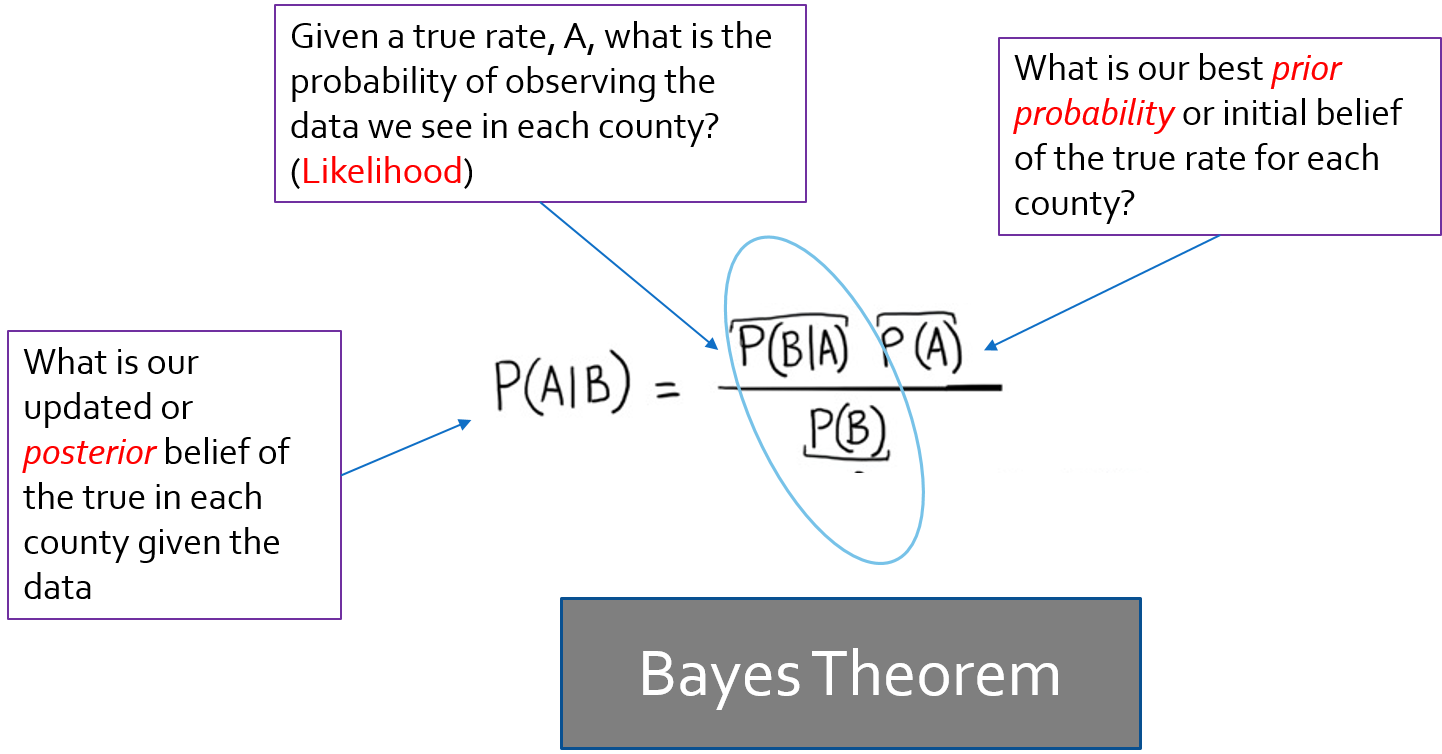
\includegraphics{images/bayes.png}
\caption{\label{fig:unnamed-chunk-87}Bayes Theorem}
\end{figure}

Bayes theorem has a familiar \emph{likelihood} component, which is essentially what we estimate from observed data. The \emph{likelihood} is the piece on which inference is based for frequentists. But for Bayesians, the theorem posits that there is some \emph{prior belief} that when combined with the \emph{likelihood} provides a new and updated \emph{posterior belief}.

While in \emph{fully Bayesian} analysis, the prior is actually a probability distribution of its own, with \emph{Empirical Bayes}, the prior is derived from some observed data. Often the prior expectation is the overall rate (either globally as it is today, or locally as it will be next week). Therefore, when we combine our prior expectation with the observed data, we can produce a statement about our updated belief in how large or small the SMR is. Because the posterior is typically not just a single number, but a fully distribution, we can also say something about precision or certainty of the estimate for each area.

\hypertarget{poisson-gamma-mixture-model}{%
\subsubsection{Poisson-Gamma mixture model}\label{poisson-gamma-mixture-model}}

Recall that the assumption of the Poisson distribution is that the \emph{mean} and the \emph{variance} are the same. But it is not uncommon that a real dataset is roughly Poisson-distributed, but perhaps because of other processes (e.g.~unmeasured predictors of the outcome) there may be extra-Poisson dispersion (e.g.~the mean \textgreater\textgreater{} variance).

This excess variation is called over-dispersion. It is a problem because it leads to biased statistical testing. You may also have learned that an alternative to the Poisson distribution is the \emph{Negative Binomial} distribution, which also works for count data, but has an extra \emph{dispersion} parameter. However instead of using the Negative binomial directly, we will look at the Poisson-Gamma mixture model, which is achieves similar ends, and is a natural fit in the Bayesian framework that is common in many disease mapping applications.

The Poisson-Gamma mixture model is a pairing of two parametric distributions to better account for squirrely data and possible extra-Poisson variance. More specifically the \emph{gamma distribution} serves as a \emph{prior} on the Poisson mean parameter, \(\theta\). In other words it describes how variable the deviations of the Poisson mean can be.

In the package \passthrough{\lstinline!SpatialEpi!}, there is a function called \passthrough{\lstinline!eBayes()!} which estimates \emph{Empirical Bayes smoothed} estimates of disease burden (or more specifically of relative excess risk or SMR), based on the Poisson-Gamma mixture.

First, let's estimate the EB-smoothed relative risk. This function expects an argument, \passthrough{\lstinline!Y!}, which is the vector of event counts, and an argument, \passthrough{\lstinline!E!}, the expected count. Note that there is also an option to include a covariate matrix, if you wanted to estimate covariate-adjusted EB-smoothed rates.

\begin{lstlisting}[language=R]
global_eb1 <- eBayes(vlbw$VLBW, vlbw$expect)
# names(global_eb1)  # look at the object returned

names(global_eb1)
\end{lstlisting}

\begin{lstlisting}
## [1] "RR"    "RRmed" "beta"  "alpha" "SMR"
\end{lstlisting}

Notice that the object \passthrough{\lstinline!global\_eb1!} that was returned by the function \passthrough{\lstinline!eBayes()!} is actually a list with 5 elements. It includes the \passthrough{\lstinline!SMR!} (which is based on observed data, not smoothed!), as well as the \passthrough{\lstinline!RR!} (mean estimate for the \emph{smoothed} relative risk), and \passthrough{\lstinline!RRmed!} (the median estimate for the \emph{smoothed} relative risk, which in our case is nearly identical to mean). Notice there are also estimates of the \(\beta\) (\passthrough{\lstinline!beta!}) and \(\alpha\) (\passthrough{\lstinline!alpha!}) parameters of the Gamma prior that were estimated from the data.

We can now add the \emph{smoothed} or \emph{stabilized} estimates to our dataset and map the \emph{raw} or \emph{unsmoothed} SMR compared to the \emph{Empirical Bayes smoothed} SMR\ldots{}

\begin{lstlisting}[language=R]
# this adds the smoothed relative risk (same as SMR) to the vlbw dataset
vlbw$ebSMR <- global_eb1$RR
\end{lstlisting}

\begin{lstlisting}[language=R]
smr_map <- tm_shape(vlbw) +
  tm_fill('SMR',
          style = 'quantile', palette = '-RdYlBu',
          title = 'Std. Morbidity Ratio') + 
  tm_borders() +
  tm_layout(main.title = 'Raw SMR of VLBW',
            inner.margins = c(0.02, 0.02, 0.1, 0.05),
            legend.format = list(digits = 2))+
  tm_shape(ga) +
  tm_borders(lwd = 2, col = 'black')

eb_map <- tm_shape(vlbw) +
  tm_fill('ebSMR',
          style = 'quantile', 
          palette = '-RdYlBu',
          title = 'Std. Morbidity Ratio') + 
  tm_borders() +
  tm_layout(main.title = 'EB smoothed SMR of VLBW',
            inner.margins = c(0.02, 0.02, 0.1, 0.05),
            legend.format = list(digits = 2))+
  tm_shape(ga) +
  tm_borders(lwd = 2, col = 'black')

tmap_arrange(smr_map, eb_map)
\end{lstlisting}

\includegraphics{EPI563-SpatialEPI_files/figure-latex/unnamed-chunk-90-1.pdf}

Each map is symbolized using an independent quantile categorization. As a result, notice two things about the map comparison above:

\begin{itemize}
\tightlist
\item
  The general patterns of highs and lows is quite similar, although not identical
\item
  The cutpoints in the legend are relatively different.
\end{itemize}

\includegraphics{EPI563-SpatialEPI_files/figure-latex/unnamed-chunk-91-1.pdf}

Looking a little more closely at the differences illustrated in the plot above we can observe several things about Empirical Bayes smoothing in relation to both population size and degree of parameter shrinkage towards the mean:

\begin{itemize}
\tightlist
\item
  The counties with the largest sample size (larger dots on plot) fall along the diagonal where the observed and smoothed rates are most similar
\item
  Conversely, the counties most likely to be `\emph{fanned out}' or off the diagonal (indicating a different value in the observed versus smoothed) were those with the smallest number of events (e.g.~small dots)
\item
  Similarly the bluer dots (those with least shrinkage) were also \emph{larger} and \emph{less extreme} in value
\item
  The redder dots (those with the most shrinkage) tended to be smaller.
\end{itemize}

\hypertarget{estimating-bayesian-exceedance-probabilities-from-poisson-gamma-eb-estimates}{%
\subsubsection{Estimating Bayesian exceedance probabilities from Poisson-Gamma EB estimates}\label{estimating-bayesian-exceedance-probabilities-from-poisson-gamma-eb-estimates}}

By estimating parameters for the Gamma-prior on the Poisson parameter, \(\theta\), we can describe not only the point estimates but actually can describe the entire posterior distribution of our estimated smooth rate. The \emph{posterior distribution} is a way of saying that in Bayesian statistics there is not just one answer, but instead a probabilistic range of answers. Whereas in \emph{frequentist} statistics we talk about \emph{confidence intervals}, in \emph{Bayesian} statistics the roughly corresponding idea is called a \textbf{credible interval}, and is essentially specific thresholds of the posterior.

The interpretation of \emph{credible intervals} is not identical to \emph{confidence intervals}, but is close enough for now. While not necessary for disease mapping, it might help for illustration to visualize the posterior estimate for two counties. One is Dekalb county, which has a large population, and the other is Baker county which had a small population. As you can see, the SMR (based on observed data) are quite different, but the mean posterior estimate of the EB-smoothed RR is nearly identical. You can also see the precision or certainty of each, with much wider (greater) uncertainty for Stewart County as compared to Dekalb county.

\includegraphics{EPI563-SpatialEPI_files/figure-latex/unnamed-chunk-92-1.pdf}

To describe how likely or unlikely the EB-smoothed relative risk for a given county is different from the null value of 1, we can use \emph{Bayesian exceedance probabilities}. These sound similar to the \emph{p-values} we mapped with the \passthrough{\lstinline!probmap()!} function, but their interpretation is different in the Bayesian framework. Specifically, instead of the somewhat convoluted way we interpret p-values (e.g.~\emph{``the probability that we would observe counts as or more extreme in infinite repeated samples, assuming the null were true''}), the Bayesian exceedance probabilities are more straightforward. Specifically it would simply be, \emph{``the probability that the true parameter, \(\theta\) is greater than 1.0, given the prior and observed data''}.

The function called \passthrough{\lstinline!EBposththreshold()!} does this calculation, and requires several arguments including the conventional observed and expected counts, but also the two parameters ,\passthrough{\lstinline!alpha!} and \passthrough{\lstinline!beta!} estimated in the previous step. We also need to specify the threshold beyond which we are interested in making inference. For a relative risk that would typically be 1.0, but if you wanted to ask about the probability of exceeding a different value (e.g.~\emph{``what is the probability that the RR is greater than 2?''}), that is an option.

\begin{lstlisting}[language=R]
vlbw$eb2_prob <- EBpostthresh(Y = vlbw$VLBW, 
                              E = vlbw$expect, 
                              alpha = global_eb1$alpha, 
                              beta = global_eb1$beta, 
                              rrthresh = 1)
\end{lstlisting}

While not necessary for disease mapping, you might be interested in how different the \emph{Bayesian} and \emph{frequentist} approach are. This plot shows that for this dataset.

\includegraphics{EPI563-SpatialEPI_files/figure-latex/unnamed-chunk-94-1.pdf}

There are two things to note about the plot comparing the two estimates of certainty or precision:

\begin{enumerate}
\def\labelenumi{\arabic{enumi}.}
\tightlist
\item
  First, it is apparent that they are \emph{inversely} related. In other words as the frequentist \emph{p-value} increases, the predictive probability from the Bayesian model gets smaller. This is simply because they are evaluating inverse parts of the same question. The \emph{frequentist p-value} is evaluating the probability of observing data more extreme than we have if the null were true (e.g.~small \emph{p-values} lend support for rejection of the null). In contrast the Bayesian exceedance probability is reporting the \emph{probability that this county has an RR greater than 1.0}. As such, a higher probability is more consistent with \emph{true} extremes, rather than spurious ones.\\
\item
  Second, they are largely consistent, albeit not identical to one another. In other words they track along a diagonal suggesting that a county with a given \emph{p-value} has a corresponding and proportionate partner in the \emph{exceedance probability}. The differences reflect the smoothing or stabilization due to the EB methods.
\end{enumerate}

\hypertarget{mapping-poisson-gamma-eb-estimates-and-exceedance}{%
\subsubsection{Mapping Poisson-Gamma EB estimates and exceedance}\label{mapping-poisson-gamma-eb-estimates-and-exceedance}}

Finally, here is a map of the smoothed estimates \textbf{and} the indication for those with high probability of being different from the Georgia average rate (e.g.~probability of exceeding SMR of 1.0 is 95\%).

\begin{lstlisting}[language=R]
# Identify counties with p-value < 0.05
pv <- vlbw %>%
  mutate(pmap.pv = ifelse(SMR > 1 & pmap < 0.05, 1, 0)) %>%
  group_by(pmap.pv) %>%
  summarise() %>%
  filter(pmap.pv == 1)


m3<- tm_shape(vlbw) +
  tm_fill('SMR',
          style = 'quantile',
          palette = '-RdYlBu',
          #breaks = c(0.13, 0.67, 0.9, 1.1, 1.4, 2.3),
          title = 'Std. Morbidity Ratio') + 
  tm_borders() +
  tm_layout(main.title = 'SMR of VLBW,\nGA 2018-2019',
            inner.margins = c(0.1, 0.02,0.05,0.2),
            legend.format = list(digits = 2)) +
  # Add dark borders for significant
  tm_shape(pv) +
  tm_borders(lwd = 2, col = 'black') +
  #tm_shape(ga) + 
  tm_borders(lwd = 1.5, col = 'black') +
  tm_credits('Counties with higher than expected risk (p<0.05) highlighted with dark borders')+
  tm_shape(ga) +
  tm_borders(lwd = 1.5, col = 'black')

# Identify counties with EB exceedance probability > 0.95 (corresponds to p<0.05)
pv2 <- vlbw %>%
  mutate(eb.pv = ifelse(ebSMR > 1 & eb2_prob > 0.95, 1, 0)) %>%
  group_by(eb.pv) %>%
  summarise() %>%
  filter(eb.pv == 1)

m4 <- tm_shape(vlbw) +
  tm_fill('ebSMR',
          style = 'quantile',
          palette = '-RdYlBu',
          #breaks = c(0.13, 0.67, 0.9, 1.1, 1.4, 2.3),
          title = 'Std. Morbidity Ratio') + 
  tm_borders() +
  tm_layout(main.title = 'Empirical Bayes smoothed\nSMR of VLBW',
            inner.margins = c(0.1, 0.02,0.05,0.2),
            legend.format = list(digits = 2)) +
  # Add dark borders for significant
  tm_shape(pv2) +
  tm_borders(lwd = 2, col = 'black') +
  tm_credits('Counties with higher than expected risk (p<0.05) highlighted with dark borders')+
  tm_shape(ga) +
  tm_borders(lwd = 1.5, col = 'black')

tmap_arrange(m3, m4)
\end{lstlisting}

\includegraphics{EPI563-SpatialEPI_files/figure-latex/unnamed-chunk-95-1.pdf}

Comparing these two maps you will see that there are \emph{fewer significant counties} using the Empirical Bayes approach. This is not surprising, and consistent with our goal of trying to separate the \emph{signal} from the \emph{random noise}. This would suggest that at least some of the counties appearing to be significantly different from the global rate, were in fact plausibly outliers with small amounts of information that cannot be stably and precisely estimated.

\hypertarget{disease-mapping-ii}{%
\chapter{Disease Mapping II}\label{disease-mapping-ii}}

\hypertarget{getting-ready-w5}{%
\section{Getting Ready, w5}\label{getting-ready-w5}}

\hypertarget{w5-learning-objectives}{%
\subsection{w5 Learning objectives}\label{w5-learning-objectives}}

 
  \providecommand{\huxb}[2]{\arrayrulecolor[RGB]{#1}\global\arrayrulewidth=#2pt}
  \providecommand{\huxvb}[2]{\color[RGB]{#1}\vrule width #2pt}
  \providecommand{\huxtpad}[1]{\rule{0pt}{#1}}
  \providecommand{\huxbpad}[1]{\rule[-#1]{0pt}{#1}}

\begin{table}[ht]
\begin{centerbox}
\begin{threeparttable}
\captionsetup{justification=centering,singlelinecheck=off}
\caption{\label{tab:learning-ob} Learning objectives by weekly module}
 \setlength{\tabcolsep}{0pt}
\begin{tabularx}{1\textwidth}{p{1\textwidth}}


\hhline{>{\huxb{255, 255, 255}{1}}-}
\arrayrulecolor{black}

\multicolumn{1}{!{\huxvb{255, 255, 255}{1}}p{1\textwidth}!{\huxvb{255, 255, 255}{1}}}{\cellcolor[RGB]{208, 211, 212}\hspace{6pt}\parbox[b]{1\textwidth-6pt-6pt}{\huxtpad{2pt + 1em}\raggedright \textbf{After this module you should be able to…}\huxbpad{2pt}}} \tabularnewline[-0.5pt]


\hhline{>{\huxb{255, 255, 255}{1}}-}
\arrayrulecolor{black}

\multicolumn{1}{!{\huxvb{255, 255, 255}{1}}p{1\textwidth}!{\huxvb{255, 255, 255}{1}}}{\cellcolor[RGB]{250, 229, 211}\hspace{6pt}\parbox[b]{1\textwidth-6pt-6pt}{\huxtpad{2pt + 1em}\raggedright Compare and contrast the operationalization of distance or contiguity in spatial statistics to sociologic and demographic theories of health relevant processes and relationships in space\huxbpad{2pt}}} \tabularnewline[-0.5pt]


\hhline{>{\huxb{255, 255, 255}{1}}-}
\arrayrulecolor{black}

\multicolumn{1}{!{\huxvb{255, 255, 255}{1}}p{1\textwidth}!{\huxvb{255, 255, 255}{1}}}{\cellcolor[RGB]{245, 203, 167}\hspace{6pt}\parbox[b]{1\textwidth-6pt-6pt}{\huxtpad{2pt + 1em}\raggedright Apply and justify contrasting definitions of spatial weights matrix in estimation of statistically smoothed disease maps\huxbpad{2pt}}} \tabularnewline[-0.5pt]


\hhline{>{\huxb{255, 255, 255}{1}}-}
\arrayrulecolor{black}
\end{tabularx}
\end{threeparttable}\par\end{centerbox}

\end{table}
 

\hypertarget{additional-resources-w5}{%
\subsection{Additional Resources, w5}\label{additional-resources-w5}}

\begin{itemize}
\tightlist
\item
  \href{https://dces.wisc.edu/wp-content/uploads/sites/128/2013/08/W14_Anselin2007.pdf}{Anselin, L. Spatial Regression Analysis in R: A workbook. 2007.}
\item
  \href{https://geodacenter.github.io/workbook/4b_dist_weights/lab4b.html}{GeoDa Center Resources: Section on distance-based spatial weights}
\item
  \href{https://geodacenter.github.io/workbook/4a_contig_weights/lab4a.html}{GeoDa Center Resources: Section on contiguity-based spatial weights}
\end{itemize}

\hypertarget{important-vocabulary-w5}{%
\subsection{Important Vocabulary, w5}\label{important-vocabulary-w5}}

 
  \providecommand{\huxb}[2]{\arrayrulecolor[RGB]{#1}\global\arrayrulewidth=#2pt}
  \providecommand{\huxvb}[2]{\color[RGB]{#1}\vrule width #2pt}
  \providecommand{\huxtpad}[1]{\rule{0pt}{#1}}
  \providecommand{\huxbpad}[1]{\rule[-#1]{0pt}{#1}}

\begin{table}[ht]
\begin{centerbox}
\begin{threeparttable}
\captionsetup{justification=centering,singlelinecheck=off}
\caption{\label{tab:unnamed-chunk-98} Vocabulary for Week 5}
 \setlength{\tabcolsep}{0pt}
\begin{tabularx}{0.9\textwidth}{p{0.45\textwidth} p{0.45\textwidth}}


\hhline{>{\huxb{255, 255, 255}{1}}->{\huxb{255, 255, 255}{1}}-}
\arrayrulecolor{black}

\multicolumn{1}{!{\huxvb{255, 255, 255}{1}}p{0.45\textwidth}!{\huxvb{255, 255, 255}{1}}}{\cellcolor[RGB]{84, 153, 199}\hspace{6pt}\parbox[b]{0.45\textwidth-6pt-2pt}{\huxtpad{2pt + 1em}\raggedright \textbf{\textcolor[RGB]{255, 255, 255}{Term}}\huxbpad{2pt}}} &
\multicolumn{1}{p{0.45\textwidth}!{\huxvb{255, 255, 255}{1}}}{\cellcolor[RGB]{84, 153, 199}\hspace{2pt}\parbox[b]{0.45\textwidth-2pt-6pt}{\huxtpad{2pt + 1em}\raggedright \textbf{\textcolor[RGB]{255, 255, 255}{Definition}}\huxbpad{2pt}}} \tabularnewline[-0.5pt]


\hhline{>{\huxb{255, 255, 255}{1}}->{\huxb{255, 255, 255}{1}}-}
\arrayrulecolor{black}

\multicolumn{1}{!{\huxvb{255, 255, 255}{1}}p{0.45\textwidth}!{\huxvb{255, 255, 255}{1}}}{\cellcolor[RGB]{212, 230, 241}\hspace{6pt}\parbox[b]{0.45\textwidth-6pt-2pt}{\huxtpad{2pt + 1em}\raggedright \textbf{Aspatial vs. Spatial}\huxbpad{2pt}}} &
\multicolumn{1}{p{0.45\textwidth}!{\huxvb{255, 255, 255}{1}}}{\cellcolor[RGB]{212, 230, 241}\hspace{2pt}\parbox[b]{0.45\textwidth-2pt-6pt}{\huxtpad{2pt + 1em}\raggedright This distinction refers to whether or not spatial proximity or contiguity is explicitly incorporated into an analysis (spatial) versus whether spatial units are treated as independent of one another (aspatial)\huxbpad{2pt}}} \tabularnewline[-0.5pt]


\hhline{>{\huxb{255, 255, 255}{1}}->{\huxb{255, 255, 255}{1}}-}
\arrayrulecolor{black}

\multicolumn{1}{!{\huxvb{255, 255, 255}{1}}p{0.45\textwidth}!{\huxvb{255, 255, 255}{1}}}{\cellcolor[RGB]{169, 204, 227}\hspace{6pt}\parbox[b]{0.45\textwidth-6pt-2pt}{\huxtpad{2pt + 1em}\raggedright \textbf{Delauney triangulation}\huxbpad{2pt}}} &
\multicolumn{1}{p{0.45\textwidth}!{\huxvb{255, 255, 255}{1}}}{\cellcolor[RGB]{169, 204, 227}\hspace{2pt}\parbox[b]{0.45\textwidth-2pt-6pt}{\huxtpad{2pt + 1em}\raggedright Geometric strategy for creating a mesh of contiguous, nonoverlapping triangles from a dataset of points. If points are the centroids of polygons, the triangle edges become graph-based definitions of spatial neighbors\huxbpad{2pt}}} \tabularnewline[-0.5pt]


\hhline{>{\huxb{255, 255, 255}{1}}->{\huxb{255, 255, 255}{1}}-}
\arrayrulecolor{black}

\multicolumn{1}{!{\huxvb{255, 255, 255}{1}}p{0.45\textwidth}!{\huxvb{255, 255, 255}{1}}}{\cellcolor[RGB]{212, 230, 241}\hspace{6pt}\parbox[b]{0.45\textwidth-6pt-2pt}{\huxtpad{2pt + 1em}\raggedright \textbf{Distance}\huxbpad{2pt}}} &
\multicolumn{1}{p{0.45\textwidth}!{\huxvb{255, 255, 255}{1}}}{\cellcolor[RGB]{212, 230, 241}\hspace{2pt}\parbox[b]{0.45\textwidth-2pt-6pt}{\huxtpad{2pt + 1em}\raggedright A fundamental dimension in geography referring to the strength of connectedness or proximity in eculidean space, social space, or network space. Distance if fundamental because we assume that a) entities that are closer are, on average, more alike than entities that are far apart; and b) increasing distance represents increasing friction or imedance to social and health-relevant interaction\huxbpad{2pt}}} \tabularnewline[-0.5pt]


\hhline{>{\huxb{255, 255, 255}{1}}->{\huxb{255, 255, 255}{1}}-}
\arrayrulecolor{black}

\multicolumn{1}{!{\huxvb{255, 255, 255}{1}}p{0.45\textwidth}!{\huxvb{255, 255, 255}{1}}}{\cellcolor[RGB]{169, 204, 227}\hspace{6pt}\parbox[b]{0.45\textwidth-6pt-2pt}{\huxtpad{2pt + 1em}\raggedright \textbf{Neighbor symmetry}\huxbpad{2pt}}} &
\multicolumn{1}{p{0.45\textwidth}!{\huxvb{255, 255, 255}{1}}}{\cellcolor[RGB]{169, 204, 227}\hspace{2pt}\parbox[b]{0.45\textwidth-2pt-6pt}{\huxtpad{2pt + 1em}\raggedright An attribute of spatial relationships in which it is assumed that if spatial unit A is a neighbor with B, then spatial unit B is also a neighbor with A. Some neighbor definitions (e.g. k-nearest neighbors) do not require symmetry.\huxbpad{2pt}}} \tabularnewline[-0.5pt]


\hhline{>{\huxb{255, 255, 255}{1}}->{\huxb{255, 255, 255}{1}}-}
\arrayrulecolor{black}

\multicolumn{1}{!{\huxvb{255, 255, 255}{1}}p{0.45\textwidth}!{\huxvb{255, 255, 255}{1}}}{\cellcolor[RGB]{212, 230, 241}\hspace{6pt}\parbox[b]{0.45\textwidth-6pt-2pt}{\huxtpad{2pt + 1em}\raggedright \textbf{Spatial neighbors}\huxbpad{2pt}}} &
\multicolumn{1}{p{0.45\textwidth}!{\huxvb{255, 255, 255}{1}}}{\cellcolor[RGB]{212, 230, 241}\hspace{2pt}\parbox[b]{0.45\textwidth-2pt-6pt}{\huxtpad{2pt + 1em}\raggedright The set of spatial entities that are determined to be 'near' rather than 'far' (in binary terms) or relatively 'closer' or 'further' (in continuous terms). The definition of 'neighbors' is part of specifying spatial relatedness.\huxbpad{2pt}}} \tabularnewline[-0.5pt]


\hhline{>{\huxb{255, 255, 255}{1}}->{\huxb{255, 255, 255}{1}}-}
\arrayrulecolor{black}

\multicolumn{1}{!{\huxvb{255, 255, 255}{1}}p{0.45\textwidth}!{\huxvb{255, 255, 255}{1}}}{\cellcolor[RGB]{169, 204, 227}\hspace{6pt}\parbox[b]{0.45\textwidth-6pt-2pt}{\huxtpad{2pt + 1em}\raggedright \textbf{Spatial weights matrix}\huxbpad{2pt}}} &
\multicolumn{1}{p{0.45\textwidth}!{\huxvb{255, 255, 255}{1}}}{\cellcolor[RGB]{169, 204, 227}\hspace{2pt}\parbox[b]{0.45\textwidth-2pt-6pt}{\huxtpad{2pt + 1em}\raggedright Typically a square matrix (n rows x n columns where n=geographic units) indexing all units on rows and columns. The values in the matrix indicate the spatial connectedness between all pairs of units.\huxbpad{2pt}}} \tabularnewline[-0.5pt]


\hhline{>{\huxb{255, 255, 255}{1}}->{\huxb{255, 255, 255}{1}}-}
\arrayrulecolor{black}

\multicolumn{1}{!{\huxvb{255, 255, 255}{1}}p{0.45\textwidth}!{\huxvb{255, 255, 255}{1}}}{\cellcolor[RGB]{212, 230, 241}\hspace{6pt}\parbox[b]{0.45\textwidth-6pt-2pt}{\huxtpad{2pt + 1em}\raggedright \textbf{Toblers' First Law of Geography}\huxbpad{2pt}}} &
\multicolumn{1}{p{0.45\textwidth}!{\huxvb{255, 255, 255}{1}}}{\cellcolor[RGB]{212, 230, 241}\hspace{2pt}\parbox[b]{0.45\textwidth-2pt-6pt}{\huxtpad{2pt + 1em}\raggedright All things are related, but near things are more related on average than distant things\huxbpad{2pt}}} \tabularnewline[-0.5pt]


\hhline{>{\huxb{255, 255, 255}{1}}->{\huxb{255, 255, 255}{1}}-}
\arrayrulecolor{black}
\end{tabularx}
\end{threeparttable}\par\end{centerbox}

\end{table}
 

\hypertarget{spatial-thinking-in-epidemiology-w5}{%
\section{Spatial Thinking in Epidemiology, w5}\label{spatial-thinking-in-epidemiology-w5}}

This is the first time where we will formally incorporate and make explicit what \emph{spatial} means in \emph{spatial analysis}. Although all work up until now has been represented on a map (thus spatially contextualized), we have not formally incorporate spatial relationships into any aspect of analysis. Specifically, last week we calculated statistical tests for heterogeneity, estimated precision or statistical significance, and produced Empirical Bayes smoothed (stabilized) estimates of parameters of interest. But each of these treated each spatial unit as it were spatially or geographically \emph{independent} of every other spatial unit. This assumption that units are geographically independent is what I have referred to as \textbf{aspatial analysis}.

\hypertarget{an-argument-for-the-relevance-of-space}{%
\subsection{An argument for the relevance of space}\label{an-argument-for-the-relevance-of-space}}

To formally and explicitly incorporate spatial relatedness we need to be clear about what constitutes spatial relationship. There are two aspects to considering spatial relatedness, and they apply to two sides of spatial thinking about health. As discussed in the recorded lecture, the fundamental dimension for spatial relations in geography is that of \emph{distance}, whether that be euclidean (e.g.~as the crow flies) distance, social distance, or network distance.

On the one hand, distance is used as a metric for defining some aspect of \emph{local population homogeneity} that is distinct from the \emph{broader regional (e.g.~study region-wide) heterogeneity}. In other words, based on Tobler's First Law of Geography, near things tend to be more alike than distant things (on average), implying a kind of dependence or correlation among local units that might not be evident overall. This concept -- which seems to hold true for many human and non-human systems -- means that when faced with sparse data, and concern for uncertainty, we can `\emph{borrow}' statistical information from spatial neighbors to supplement estimation of local disease parameters. This is exactly what we will do with \emph{spatial Empirical Bayes} estimation, where instead of using the overall (global) rate of disease as the prior, we will use the \emph{local rate} for neighbors surrounding each entity as a kind of custom, place-specific prior.

But at a deeper level, distance is also important to spatial thinking in epidemiology. This is because we hypothesize -- and are interested in -- whether entities that are geographically or socially more connected share health-relevant experiences. These experiences or exposures include microbial space (e.g.~person-to-person transmission of infectious agents), social norms (e.g.~acceptability of smoking or body image perceptions), built environments (e.g.~lead exposure in municipal water systems, food environments), access to health resources (e.g.~health care, cancer screening), and access to opportunity structures (e.g.~good schools, safe streets, employment opportunities).

The examples above rely primarily on the note of \emph{distance} in Cartesian (geographic) space. However, it is worth emphasizing how more complex versions of \emph{distance} and \emph{proximity} could come into play. For example air travel makes the \emph{distance} between two places less relevant than the economic and social drivers of flows of people back and forth when it comes to infectious disease transmission such as Zika or Ebola. There is a still a \emph{distance} dimension, but it is defined by the push and pull of human mobility and migration. It is possible to define \emph{spatial neighbors} in these more abstract (e.g.~non-geographic) ways. For example, political scientists have created spatial weights matrices that connect states not by their geographic boundaries, but by how similarly their legislatures act on policy decisions. In this way \emph{distance} is a measure of ideology rather than geography, but still has meaning for spatial analysis of health. But for today we will focus on the more specific example of \emph{geographic space} rather than social, political, or economic \emph{space}.

In sum, the notion of explicitly \emph{spatial analysis} is a way to incorporate theoretical and conceptual aspects of how humans relate to one another and their environment into our understanding of the distribution and determinants of disease.

Whether we treat spatial dependence and relatedness as a primarily statistical feature for exploitation (e.g.~as in spatial disease mapping with Empirical Bayes), or as an attribute of the local ecosystem of disease generation, it is clear that when and how neighbors are defined is influential on the final numerical results and the inference we take from them. The definition of spatial neighbors, and the corresponding symbolization of that relatedness with creation of spatial weights matrices is a fundamental bridge between theory of geography and meaning for spatial epidemiology.

\hypertarget{on-making-meaning-from-neighbors}{%
\subsection{On making meaning from neighbors}\label{on-making-meaning-from-neighbors}}

The challenge for the spatial epidemiologist is twofold:
1. Conceptualizing the spatial scale and extent at which a health relevant process of interest occur
2. Translating that conceptual idea to an explicit definition of neighbors, and therefore spatial weights

For areal analysis (e.g.~spatial analysis of polygons), there are two broad classes of neighborhood definitions: contiguity-based definitions and distance-based definitions. In reality both are abstract expressions of `distance', but they differ in how `\emph{near}' and `\emph{far}' are operationalized. While we are primarily focused on analysis of areal units in this course, it is possible to create neighbor definitions among point-referenced data by using a tessalation process such as creation of Thiessen polygons (e.g.~see \href{https://geodacenter.github.io/workbook/4b_dist_weights/lab4b.html\#distance-metric}{this discussion on Contiguity-based weights for points}). Below is a brief summary of several common neighbor definitions:

\begin{longtable}[]{@{}lll@{}}
\toprule
\begin{minipage}[b]{0.13\columnwidth}\raggedright
\strut
\end{minipage} & \begin{minipage}[b]{0.14\columnwidth}\raggedright
Basic metric\strut
\end{minipage} & \begin{minipage}[b]{0.63\columnwidth}\raggedright
Description\strut
\end{minipage}\tabularnewline
\midrule
\endhead
\begin{minipage}[t]{0.13\columnwidth}\raggedright
\textbf{Rook}\strut
\end{minipage} & \begin{minipage}[t]{0.14\columnwidth}\raggedright
Contiguity\strut
\end{minipage} & \begin{minipage}[t]{0.63\columnwidth}\raggedright
Unit A and unit B are neighbors if and only if they share boundary edges. Second or higher-order contiguity refers to units sharing edges with index unit (1st order contiguity), plus units that share boundary edges with all 1st order neighbors; and so forth)\strut
\end{minipage}\tabularnewline
\begin{minipage}[t]{0.13\columnwidth}\raggedright
\textbf{Queen}\strut
\end{minipage} & \begin{minipage}[t]{0.14\columnwidth}\raggedright
Contiguity\strut
\end{minipage} & \begin{minipage}[t]{0.63\columnwidth}\raggedright
Unit A and unit B are neighbors if they share \emph{either} boundary edges \emph{or} boundary corners (e.g.~vertices). Second or higher-order contiguity refers to units sharing edges with index unit (1st order contiguity), plus units that share boundary edges with all 1st order neighbors; and so forth)\strut
\end{minipage}\tabularnewline
\begin{minipage}[t]{0.13\columnwidth}\raggedright
\textbf{Sphere of influence graph neighbors}\strut
\end{minipage} & \begin{minipage}[t]{0.14\columnwidth}\raggedright
Contiguity\strut
\end{minipage} & \begin{minipage}[t]{0.63\columnwidth}\raggedright
\emph{Graph-based} neighbors start by creating \emph{Delauney triangles} from the centroid of units. Neighbors are defined by the \emph{edges} of the triangles.\strut
\end{minipage}\tabularnewline
\begin{minipage}[t]{0.13\columnwidth}\raggedright
\textbf{Fixed distance}\strut
\end{minipage} & \begin{minipage}[t]{0.14\columnwidth}\raggedright
Distance\strut
\end{minipage} & \begin{minipage}[t]{0.63\columnwidth}\raggedright
Unit A is a neighbor of unit B, if unit A (or perhaps the centroid of the unit) falls within a fixed-distance buffer created around unit B (or perhaps the centroid of the unit).\strut
\end{minipage}\tabularnewline
\begin{minipage}[t]{0.13\columnwidth}\raggedright
\textbf{K-nearest neighbors (KNN)}\strut
\end{minipage} & \begin{minipage}[t]{0.14\columnwidth}\raggedright
Distance\strut
\end{minipage} & \begin{minipage}[t]{0.63\columnwidth}\raggedright
Unit A is a neighbor of unit B, if when a rank-order of closest to furthest neighbors from Unit B is created, Unit A is ranked \(\leq k\). In other words, if \(K\) is set to 5, then unit A is neighbor of B if it is among the 5 nearest neighbors. KNN is an \emph{asymmetric} definition; it is possible for A to be neighbors with B, but B may not be a neighbor to A.\strut
\end{minipage}\tabularnewline
\begin{minipage}[t]{0.13\columnwidth}\raggedright
\textbf{Inverse distance}\strut
\end{minipage} & \begin{minipage}[t]{0.14\columnwidth}\raggedright
Distance\strut
\end{minipage} & \begin{minipage}[t]{0.63\columnwidth}\raggedright
Instead of using a fixed threshold of distance (e.g.~a buffer) or a fixed number of near neighbors (e.g.~KNN), this strategy describes proximity or `\emph{nearness}' as the inverse of the Euclidean or road-network distance (or possibly inverse of distance-squared).\strut
\end{minipage}\tabularnewline
\bottomrule
\end{longtable}

The choice of which neighbor definition to use is influenced by several study-specific factors, some of which can be in conflict with others:

\begin{itemize}
\tightlist
\item
  Variation in size of areal units across the study area. If some areal units are very small (e.g.~counties in the Eastern U.S.) and some are very large (e.g.~counties in the Western U.S.), then the geographic area defined by adjacent counties will be quite different. In contrast, fixed-distance neighbors will be more consistent.
\item
  Assumptions or requirements of the statistical analysis of interest. Some algorithms require/expect features such as \emph{neighbor symmetry} or \emph{spatial weights row standardization} to account for unequal numbers of neighbors.
\item
  The assumed meaning of space in the analysis. It is possible that, for instance, the meaning of distance in Western counties is different where further travel to basic services is more the norm than in denser areas in the East.
\item
  The purpose and audience of the map. It is important to make the analysis accessible and interpretable to the target audience.
\item
  Aspects of the geography including islands or presence of non-contiguous units (e.g.~Hawaii, Alaska, Puerto Rico)
\end{itemize}

\hypertarget{spatial-analysis-in-epidemiology-w5}{%
\section{Spatial Analysis in Epidemiology, w5}\label{spatial-analysis-in-epidemiology-w5}}

To apply these concepts to specific spatial analysis, we will continue to use the Georgia \emph{very low birthweight} dataset used in the previous module of the eBook. As a reminder, this is a county-level dataset for the \(n=159\) Georgia Counties containing the county of all live births (denominator) as well as the count of VLBW births (weight at birth \textless{} 1500 grams) babies in 2018-2019. These data were derived from the \href{https://oasis.state.ga.us/}{Georgia OASIS website}.

In this section we first introduce how to create and examine several different spatial neighbor definitions. But we never create neighbors just or their own sake. The purpose of creating spatial neighbors and weights matrices is always to use the definition in a spatial analysis. Later in this section you will see the use of the spatial weights for producing \emph{spatial Empirical Bayes} estimates.

\hypertarget{creating-contiguity-neighbor-objects}{%
\subsection{Creating contiguity neighbor objects}\label{creating-contiguity-neighbor-objects}}

In \passthrough{\lstinline!R!}, the \passthrough{\lstinline!spdep!} package has a series of functions useful for creating spatial weights matrices. In general, the process of going from a spatial object (e.g.~an \passthrough{\lstinline!sf!} class data object) to a usable spatial weights matrix requires more than one step, and the steps vary depending on the eventual use.

Since we are starting with areal (polygon) data, the starting point is to use a utility function, \passthrough{\lstinline!poly2nb()!}, that take a polygon spatial object (of class \passthrough{\lstinline!sf!} or \passthrough{\lstinline!sp!}) and determine which specific polygon regions are contiguous with (touch, share boundaries with) other regions. If you review the help documentation, you will see that the function takes a spatial \passthrough{\lstinline!sf!} object as the input, with arguments specifying whether to use \emph{Queen} contiguity (default; \emph{Rook} is the alternative). The function returns something called a \emph{neighbor list}.

\begin{lstlisting}[language=R]
# load the package spdep
library(spdep)

# Create a queen contiguity neighbor list
queen_nb <- poly2nb(vlbw, queen = TRUE)

# Examine the resulting object
summary(queen_nb)
\end{lstlisting}

\begin{lstlisting}
## Neighbour list object:
## Number of regions: 159 
## Number of nonzero links: 860 
## Percentage nonzero weights: 3.401764 
## Average number of links: 5.408805 
## Link number distribution:
## 
##  1  2  3  4  5  6  7  8  9 10 
##  1  4 12 29 36 37 28  9  1  2 
## 1 least connected region:
## 64 with 1 link
## 2 most connected regions:
## 1 66 with 10 links
\end{lstlisting}

The \passthrough{\lstinline!summary()!} function for objects of class \passthrough{\lstinline!nb!} (a \emph{neighbor} object created in \passthrough{\lstinline!spdep!}) provides some useful high-level info, including the presence of regions with zero links (no neighbors -- a problem that could occur with islands, for example), and the distribution of number of links or neighbors. You might want to look at the structure of the \passthrough{\lstinline!queen\_nb!} object also, either using \passthrough{\lstinline!str(queen\_nb)!}, or perhaps just viewing the first few elements in the list (e.g.~because \passthrough{\lstinline!nb!} objects are of class \passthrough{\lstinline!list!} in R, use the double-bracket indexing of lists like this \passthrough{\lstinline!queen\_nb[[1]]!}).

The neighbor object is essentially a list with length equal to the number of regions (\(n=159\) counties in this case). The elements in the list correspond to the order of the input dataset, with the first list item being the first county in the current sort order. Each element in the list is a vector identifying \emph{which other} counties are neighbors to it.

One important attribute of spatial relationships is whether they are \emph{symmetric} or not. In the context of spatial neighbors, spatial symmetry implies that if \(region_i\) is a neighbor to \(region_j\), then \(region_j\) is also a neighbor to \(region_i\). Contiguity neighbors are symmetric by design: if the definition of \emph{neighbor} is shared boundaries, that is true for either partner in the relationship. We will see below that not all definitions of spatial relationships and neighbors result in symmetric relationships. A quick way to check whether a neighbor object is symmetric or not is this code:

\begin{lstlisting}[language=R]
is.symmetric.nb(queen_nb)
\end{lstlisting}

\begin{lstlisting}
## [1] TRUE
\end{lstlisting}

To better understand a set of spatial relationships, it can be useful to visualize neighbor links or connections when choosing among a neighbor definition, simply to see the relative density and pattern of connectivity. Note that the function \passthrough{\lstinline!plot.nb()!} has the \passthrough{\lstinline!nb!} object as its first argument, but must also include a matrix of centroids as the second argument. The reason is that the \passthrough{\lstinline!nb!} object defines \emph{which} region connects to \emph{which}, but does not say where they are in space. The centroids tell the plot \emph{where} each link or line begins and ends.

\begin{lstlisting}[language=R]
# Create a matrix of the x,y coordinates for each county centroid
ga_cent <- st_centroid(st_geometry(vlbw))

# Plot the outlines of counties with light grey boundaries
plot(st_geometry(vlbw), border = 'grey')

# Add the plot of the Queen contiguity connections
plot.nb(queen_nb, ga_cent, points = F, add = T)
\end{lstlisting}

\includegraphics{EPI563-SpatialEPI_files/figure-latex/unnamed-chunk-102-1.pdf}

Notice how the density of neighbors is generally lower on the coast and at state boundaries. This systematic difference in neighbors can produce patterns sometimes referred to as \emph{edge effects}. These edge effects could be a source of bias, because counties in the interior of the state have more neighbors (and thus more `\emph{local information}' on average) than border counties. This is especially true when the absence of neighbors is artificial as in the case of counties bordering Alabama, Tennessee, North or South Carolina, Florida. In contrast, counties on the coast have a `\emph{real}' absence of neighbors.

\hypertarget{creating-k-nearest-neighbors}{%
\subsection{Creating k-nearest neighbors}\label{creating-k-nearest-neighbors}}

\emph{K-nearest neighbors} is a flexible approach to assuring balanced number of neighbors, and can help when the size and density of the spatial regions varies across the study area. For instance a fixed-distance buffer (e.g.~perhaps counties within 50 miles) might work to identify relevant neighbors in the Eastern or Midwestern U.S., but in the West, where a county may be 100-200 miles across, there would be \emph{zero} neighbors with this definition. But with \emph{K-nearest neighbors}, both smaller Eastern and larger Western counties would have neighbors (albeit of differing spatial scales).

\begin{rmdnote}
Because \emph{k-nearest neighbors} does not depend on either arbitrary fixed distance, nor on contiguity, it will always produce neighbors even for islands. For example in analyses of U.S. states, Alaska and Hawaii have no contiguous neighbors. However, a k-nearest neighbor approach would still assign the \emph{nearest neighbor} regardless of how far away. For instance the nearest neighbor to Hawaii might be California. The question you must ask yourself is whether it is meaningful to say Hawaii and California are neighbors. If you are interested in food environment, that seems implausible. However, there is a great deal of social, cultural, and economic interaction between Hawaii and California; so in some instances this could be a plausible and meaningful connection.
\end{rmdnote}

To create a \emph{k-nearest neighbor} object, we first must identify the relative proximity of candidate neighbors. To define \emph{who is nearest to whom}, by convention we measure Euclidean distance between the \emph{centroids} of polygons (literally the geometric center), under the assumption that this is an \emph{average} location to describe the polygon. This requires two steps.

First, the \passthrough{\lstinline!knearneigh()!} function takes these centroids, calculates all pair-wise distances, sorts them from closest to furthest, and then selects the \(k\) nearest (or smallest distance) units. Then the \passthrough{\lstinline!knn2nb()!} function takes this information and creates a formal \passthrough{\lstinline!nb!} or \emph{neighbor} object.

\begin{lstlisting}[language=R]
# First create two sets of neighbors: 2 nearest and 5 nearest
knn2 <- knearneigh(ga_cent, k = 2)
knn5 <- knearneigh(ga_cent, k = 5)

# Now take those lists of neighbors and make an nb object
knn2_nb <- knn2nb(knn2, row.names = vlbw$GEOID)
knn5_nb <- knn2nb(knn5, row.names = vlbw$GEOID)

summary(knn5_nb)
\end{lstlisting}

\begin{lstlisting}
## Neighbour list object:
## Number of regions: 159 
## Number of nonzero links: 795 
## Percentage nonzero weights: 3.144654 
## Average number of links: 5 
## Non-symmetric neighbours list
## Link number distribution:
## 
##   5 
## 159 
## 159 least connected regions:
## 13121 13029 13135 13127 13271 13279 13301 13007 13143 13221 13137 13289 13105 13051 13073 13189 13103 13319 13209 13317 13241 13033 13261 13249 13309 13113 13123 13157 13215 13311 13265 13019 13291 13171 13263 13001 13303 13027 13305 13133 13251 13163 13195 13013 13153 13205 13025 13009 13021 13217 13213 13151 13185 13181 13313 13183 13031 13245 13141 13191 13049 13079 13283 13083 13139 13107 13179 13229 13075 13267 13039 13077 13219 13315 13285 13095 13115 13225 13045 13035 13161 13097 13071 13237 13081 13011 13109 13017 13255 13197 13003 13015 13275 13211 13235 13131 13065 13293 13287 13155 13227 13173 13223 13277 13145 13297 13129 13295 13055 13165 13243 13047 13233 13187 13117 13111 13063 13067 13207 13101 13167 13193 13239 13149 13069 13125 13085 13091 13201 13061 13321 13169 13281 13299 13037 13053 13307 13273 13159 13023 13093 13177 13257 13175 13269 13059 13089 13043 13147 13057 13231 13253 13087 13005 13119 13247 13099 13199 13259 with 5 links
## 159 most connected regions:
## 13121 13029 13135 13127 13271 13279 13301 13007 13143 13221 13137 13289 13105 13051 13073 13189 13103 13319 13209 13317 13241 13033 13261 13249 13309 13113 13123 13157 13215 13311 13265 13019 13291 13171 13263 13001 13303 13027 13305 13133 13251 13163 13195 13013 13153 13205 13025 13009 13021 13217 13213 13151 13185 13181 13313 13183 13031 13245 13141 13191 13049 13079 13283 13083 13139 13107 13179 13229 13075 13267 13039 13077 13219 13315 13285 13095 13115 13225 13045 13035 13161 13097 13071 13237 13081 13011 13109 13017 13255 13197 13003 13015 13275 13211 13235 13131 13065 13293 13287 13155 13227 13173 13223 13277 13145 13297 13129 13295 13055 13165 13243 13047 13233 13187 13117 13111 13063 13067 13207 13101 13167 13193 13239 13149 13069 13125 13085 13091 13201 13061 13321 13169 13281 13299 13037 13053 13307 13273 13159 13023 13093 13177 13257 13175 13269 13059 13089 13043 13147 13057 13231 13253 13087 13005 13119 13247 13099 13199 13259 with 5 links
\end{lstlisting}

Notice how the summaries are not so interesting when we force everyone to have the same number of links! However in checking the symmetry, and important concern rises:

\begin{lstlisting}[language=R]
is.symmetric.nb(knn2_nb)
\end{lstlisting}

\begin{lstlisting}
## [1] FALSE
\end{lstlisting}

\begin{lstlisting}[language=R]
is.symmetric.nb(knn5_nb)
\end{lstlisting}

\begin{lstlisting}
## [1] FALSE
\end{lstlisting}

\emph{K-nearest neighbors} will almost always produce \emph{asymmetric} neighbors. Thinking about U.S. states is perhaps an easy way to understand this. Consider the state of Hawaii: the nearest states are probably California, Oregon, and Washington. However the inverse is not true. The nearest 2 (or 3 or 4 or 5) states to California are all in the contiguous `lower 48' states; Hawaii is certainly not among the \emph{nearest} places to California.

This \emph{asymmetry} is not a problem for spatial analytic tasks including the spatial Empirical Bayes smoothing we will do in this week. However, for some cluster analysis or other analyses in future weeks, neighbor symmetry is assumed and required. If you choose a \emph{k-nearest neighbor} definition, but you also require symmetric spatial relationships, you can force symmetry in at least two ways. First, you could specify \passthrough{\lstinline!sym  = TRUE!} in the \passthrough{\lstinline!knn2nb()!} call above. That essentially \emph{breaks} the rigid \emph{k-nearest neighbors} and forces reciprocity in \emph{`neighborliness'}. The second method is appropriate if you have already created \emph{asymmetric} neighbors, but wish to retrospectively force symmetry: \passthrough{\lstinline!make.sym.nb()!}. This simply takes an asymmetric neighbor object and adds links to make the relationships symmetric. Note, however, that this alters the number of links or neighbors for each region: some will now have more than others.

\begin{lstlisting}[language=R]
knn5_symmetric <- make.sym.nb(knn5_nb)
summary(knn5_symmetric)
\end{lstlisting}

\begin{lstlisting}
## Neighbour list object:
## Number of regions: 159 
## Number of nonzero links: 910 
## Percentage nonzero weights: 3.599541 
## Average number of links: 5.72327 
## Link number distribution:
## 
##  5  6  7  8 
## 73 61 21  4 
## 73 least connected regions:
## 13121 13135 13127 13289 13105 13051 13103 13319 13317 13241 13033 13249 13113 13157 13215 13171 13027 13133 13251 13013 13009 13021 13181 13031 13245 13049 13079 13083 13107 13179 13267 13039 13219 13315 13285 13095 13225 13081 13017 13275 13235 13155 13145 13295 13055 13165 13243 13047 13233 13111 13207 13101 13167 13239 13149 13091 13201 13061 13281 13053 13159 13093 13177 13257 13175 13059 13147 13057 13231 13253 13087 13005 13099 with 5 links
## 4 most connected regions:
## 13007 13223 13129 13187 with 8 links
\end{lstlisting}

\begin{lstlisting}[language=R]
is.symmetric.nb(knn5_symmetric)
\end{lstlisting}

\begin{lstlisting}
## [1] TRUE
\end{lstlisting}

Note that now there are four counties with 8 links, rather than 5. That means each of those counties were the \emph{nearest} to at least 3 others, even though those 3 were not \emph{nearest} to them.

\hypertarget{visualizing-differences-between-competing-neighbor-definitions}{%
\subsubsection{Visualizing differences between competing neighbor definitions}\label{visualizing-differences-between-competing-neighbor-definitions}}

As a spatial analyst, you might be very interested in how the choice of neighbors affects your results. To better understand what is different from one definition to the next it can be helpful to visualize them side-by-side.

Using just base-R plotting (you could create fancier maps if desired with \passthrough{\lstinline!ggplot!} or \passthrough{\lstinline!tmap!}), we can easily visualize the county polygons, with lines connecting the centroids of \emph{neighboring counties} as an indication of shared influence, contact, or interaction.

The function \passthrough{\lstinline!plot.nb()!} requires the spatial neighbor object (e.g.~object of class \passthrough{\lstinline!nb!}), a matrix of the \(x, y\) locations of polygon centroids, and then does the work of drawing the connecting lines.

The function in the code below named \passthrough{\lstinline!diffnb()!} is simply a utility function to compare two \passthrough{\lstinline!nb!} objects to determine what is the \emph{same} and what is \emph{different}. We can then plot the \emph{different} values in red in order to quickly see what differs from one neighbor definition to the next.

\begin{lstlisting}[language=R]
par(mfrow = c(1, 3),        # set plotting space for 3 side-by-side plots
    mar = c(.2,.2,1,.2))    # Set margins for plotting

# Plot the knn = 2 neighbor connections
plot(st_geometry(vlbw), border = 'grey', main = 'knn = 2')
plot.nb(knn2_nb, ga_cent, point = F, add = T)

# Plot the knn = 5 neighbor connections
plot(st_geometry(vlbw), border = 'grey', main = 'knn = 5')
plot.nb(knn5_nb, ga_cent, point = F, add = T, col = 'blue')
plot.nb(diffnb(knn2_nb, knn5_nb), ga_cent, point = F, add = T, col = 'red')

# Plot the knn = 5 AND the differences (in red) when knn = 5 is made symmetric
plot(st_geometry(vlbw), border = 'grey', main = 'Symmetric Knn5')
plot.nb(knn5_nb, ga_cent, point = F, add = T, col = 'blue')
plot.nb(diffnb(knn5_nb, knn5_symmetric), ga_cent, point = F, add = T, col = 'red')
\end{lstlisting}

\includegraphics{EPI563-SpatialEPI_files/figure-latex/unnamed-chunk-107-1.pdf}

\begin{lstlisting}[language=R]
par(mfrow = c(1,1))
\end{lstlisting}

It is no surprise that there are lots of red lines on the \emph{knn5} as compared with the \emph{knn2}. Every single county has 3 additional neighbors in the former compared to the latter. However it is interesting to see how many initially \emph{asymmetric} relationships had to have added links in order to enforce \emph{symmetry} (e.g.~the red lines in the right-hand plot, compared to middle).

\hypertarget{creating-graph-based-triangle-neighbor-objects}{%
\subsection{Creating Graph-based triangle neighbor objects}\label{creating-graph-based-triangle-neighbor-objects}}

The contiguity framework takes the reasonable approach that \emph{local} implies direct interaction as indicated by shared borders. However in many instances, the odd shape of polygons means that regions could be quite close to one another but not share a border. A different approach -- one of two methods we'll discuss called \emph{graph-based neighbors} -- defines the local neighbors by relative proximity using a geometry approach. The process subdivides the space into non-overlapping triangles, using the centroids of each region as vertices in the triangle. A \emph{neighbor} is therefore any region that is connected by an edge (link) between two vertices (centroids). More practically, this results in neighbor region that are near(ish) but are not required to have touching-borders. Graph-based neighbor objects are symmetric by design.

\begin{lstlisting}[language=R]
tri_nb <- tri2nb(ga_cent)
summary(tri_nb)
\end{lstlisting}

\begin{lstlisting}
## Neighbour list object:
## Number of regions: 159 
## Number of nonzero links: 918 
## Percentage nonzero weights: 3.631185 
## Average number of links: 5.773585 
## Link number distribution:
## 
##  3  4  5  6  7  8 
##  1 18 40 63 31  6 
## 1 least connected region:
## 15 with 3 links
## 6 most connected regions:
## 58 65 82 107 118 120 with 8 links
\end{lstlisting}

\begin{lstlisting}[language=R]
is.symmetric.nb(tri_nb)
\end{lstlisting}

\begin{lstlisting}
## [1] TRUE
\end{lstlisting}

Look back at the summary for the \passthrough{\lstinline!queen\_nb!} object created previously. This graph-based neighbor definition results in slightly more connections for every county as compared with Queen contiguity, but also reduces the variation in number of links. The Queen had counties with as many as 10 links and some with only 1 link; in contrast this graph-based definition results in counties ranging from a minimum of 3 neighbors to a maximum of 8.

To visualize the triangularized neighbors we can plot their links, next to the \emph{Queen contiguity} to compare.

\begin{lstlisting}[language=R]
par(mfrow = c(1, 2),        # set plotting space for 2 side-by-side plots
    mar = c(.2,.2,1,.2))    # Set margins for plotting

plot(st_geometry(vlbw), border = 'grey', main = 'Queen contiguity') # plot the polygons
plot.nb(queen_nb, ga_cent, add = T, points = F, col = 'blue') # plot the Queen neighbor links

plot(st_geometry(vlbw), border = 'grey', main = 'Triangle neighbors')
plot.nb(queen_nb, ga_cent, add = T, points = F, col = 'blue')
plot.nb(diffnb(queen_nb, tri_nb), ga_cent, add = T, points = F, col = 'red')
\end{lstlisting}

\includegraphics{EPI563-SpatialEPI_files/figure-latex/unnamed-chunk-109-1.pdf}

\begin{lstlisting}[language=R]
par(mfrow = c(1,1))  # This just resets the graphic device to be 1-plot per page
\end{lstlisting}

Notice how the graph-based neighbors have strange connections along the Western border of Georgia. This is because the Delauney triangle algorithm makes unexpected connections between centroids along edges. If we thought these were unreasonable spatial relationships (I think they are!), we can \emph{prune} them down by using a \emph{Sphere of Influence} graph to restrict to more proximate relationships. In most instances, carrying out this pruning to produce \emph{sphere of influence} graph neighbors is most sensible as compared to using the product we have at this stage.

The code is a little intimidating looking: It includes some nested functions where the original triangle neighbor object is fed into the \passthrough{\lstinline!soi.graph()!} function, which itself is fed into the \passthrough{\lstinline!graph2nb()!} function. But basically what it is doing is looking for ties or connections defined by the triangularization algorithm that are also proximate.

\begin{lstlisting}[language=R]
soi_nb <- graph2nb(soi.graph(tri_nb, ga_cent))

summary(soi_nb)
\end{lstlisting}

\begin{lstlisting}
## Neighbour list object:
## Number of regions: 159 
## Number of nonzero links: 850 
## Percentage nonzero weights: 3.362209 
## Average number of links: 5.345912 
## Link number distribution:
## 
##  3  4  5  6  7  8 
## 11 35 32 53 25  3 
## 11 least connected regions:
## 14 15 21 64 71 87 96 120 123 124 152 with 3 links
## 3 most connected regions:
## 65 82 107 with 8 links
\end{lstlisting}

To see how \emph{Queen} neighbors compares to each we can plot them:

\begin{lstlisting}[language=R]
par(mfrow = c(1, 3),        # set plotting space for 3 side-by-side plots
    mar = c(.2,.2,1,.2))    # Set margins for plotting

# Plot Queen
plot(st_geometry(vlbw), border = 'grey', main = 'Triangle neighbors') # plot the polygons
plot.nb(queen_nb, ga_cent, add = T, points = F, col = 'blue') # plot the Queen neighbor links


# Plot triangle and differences from Queen
plot(st_geometry(vlbw), border = 'grey', main = 'Triangle neighbors') 
plot.nb(queen_nb, ga_cent, add = T, points = F, col = 'blue') 
plot.nb(diffnb(tri_nb, queen_nb), ga_cent, add = T, points = F, col = 'red') 

# Plot Sphere of Influence and differences from Queen
plot(st_geometry(vlbw), border = 'grey', main = 'Sphere of Influence pruning')
plot.nb(queen_nb, ga_cent, add = T, points = F, col = 'blue') 
plot.nb(diffnb(queen_nb, soi_nb), ga_cent, add = T, points = F, col = 'red') 
\end{lstlisting}

\includegraphics{EPI563-SpatialEPI_files/figure-latex/unnamed-chunk-111-1.pdf}

\begin{lstlisting}[language=R]
par(mfrow = c(1,1))  # This just resets the graphic device to be 1-plot per page
\end{lstlisting}

\hypertarget{creating-fixed-distance-neighbors}{%
\subsection{Creating fixed-distance neighbors}\label{creating-fixed-distance-neighbors}}

The concept of \emph{buffering} around locations to define exposure is probably familiar. It is not uncommon for exposures such as access to health services, healthy food stores, or exposure to toxin emitters is quantified using fixed-distance buffers. The fixed-distance neighbor definition is therefore a natural extension, where we believe that the definition of \emph{local} or \emph{near} can be described by who (or where) falls within a given radius. In that way it is different from all of the previous approaches because neither sharing borders, nor being the k-nearest neighbor is required. All that is required is that the place (or more specifically the centroid of the place), falls within the designated distance. The number of other units falling within a given threshold could range from zero to the maximum number of units in the study, and certainly could vary from one location to another (e.g.~thinking again about distinctions between Easter and Western counties in the U.S.).

Determining an appropriate distance can be challenging unless there is clear theory or evidence (e.g.~the distance required to avoid exposure to radiation from a fixed point source). Often analysts consider a range of distances to understand how or whether the pattern changes under competing scenarios. This approach will be used more when we investigate spatial clusters of disease.

To define fixed-distance neighbors, we use the function \passthrough{\lstinline!dnearneigh()!} and must define both a minimum distance (probably but not always set at zero), and a maximum distance defining the buffer.

\begin{rmdcaution}
Note that the distance parameters are described on the \emph{scale of the coordinate measures of the spatial object}. In this case, the spatial object is projected, and the units are meters. Therefore a distance of 1000 is 1 kilometer. However, beware of using distance measures for unprojected data, as the units are the somewhat opaque angular degrees.
\end{rmdcaution}

Here we calculate neighbors for two distance buffers: all counties within 25km and all within 50km of the centroid of each county are neighbors; all other counties are not neighbors. Notice that the output of each instance of \passthrough{\lstinline!dnearneigh()!} is not just the distances themselves, but is actually a formal neighbor (\passthrough{\lstinline!nb!}) object.

\begin{lstlisting}[language=R]
dist_25 <- dnearneigh(ga_cent, d1 = 0, d2 = 25000)
dist_50 <- dnearneigh(ga_cent, d1 = 0, d2 = 50000)
summary(dist_50)
\end{lstlisting}

\begin{lstlisting}
## Neighbour list object:
## Number of regions: 159 
## Number of nonzero links: 1072 
## Percentage nonzero weights: 4.240339 
## Average number of links: 6.742138 
## Link number distribution:
## 
##  3  4  5  6  7  8  9 10 11 12 
## 10 18 20 21 33 21 21 10  4  1 
## 10 least connected regions:
## 4 14 22 41 61 71 96 120 152 153 with 3 links
## 1 most connected region:
## 156 with 12 links
\end{lstlisting}

We can compare the linkages of these two distance bands to one another:

\begin{lstlisting}[language=R]
par(mfrow = c(1, 2),        # set plotting space for 2 side-by-side plots
    mar = c(.2,.2,1,.2))    # Set margins for plotting


# Plot neighbor relations for 25 km
plot(st_geometry(vlbw), border = 'grey', main = '25 km neighbors')
plot.nb(dist_25, ga_cent, points = F, add = T)

# Plot neighbor relations for 50 km
plot(st_geometry(vlbw), border = 'grey', main = '50 km neighbors')
plot.nb(dist_50, ga_cent, points = F, add = T)
\end{lstlisting}

\includegraphics{EPI563-SpatialEPI_files/figure-latex/unnamed-chunk-114-1.pdf}

\begin{lstlisting}[language=R]
par(mfrow = c(1,1))
\end{lstlisting}

Or we could compare one to a previous definition (e.g.~the \emph{Queen contiguity}).

\begin{lstlisting}[language=R]
par(mfrow = c(1, 2),        # set plotting space for 2 side-by-side plots
    mar = c(.2,.2,1,.2))    # Set margins for plotting

# Plot queen for reference
plot(st_geometry(vlbw), border = 'grey', main = 'Queen')
plot.nb(queen_nb, ga_cent, points = F, add = T, col = 'blue')

# Plot the difference between queen and dist_50
plot(st_geometry(vlbw), border = 'grey', main = 'Difference of Queen & 50-km dist')
plot.nb(queen_nb, ga_cent, points = F, add = T, col = 'blue')
plot.nb(diffnb(queen_nb, dist_50), ga_cent, points = F, add = T, col = 'red')
\end{lstlisting}

\includegraphics{EPI563-SpatialEPI_files/figure-latex/unnamed-chunk-115-1.pdf}

\begin{lstlisting}[language=R]
par(mfrow = c(1,1))
\end{lstlisting}

\hypertarget{from-spatial-neighbors-to-spatial-disease-mapping}{%
\subsection{From spatial neighbors to spatial Disease Mapping}\label{from-spatial-neighbors-to-spatial-disease-mapping}}

The main reason for struggling through all of the preceding ins and outs of spatial neighbors is because we would like to define a reasonable version of \emph{local} given a spatial dataset, and use that definition to advance spatial epidemiologic goals. As discussed above, a primary goal is the production of statistically stable rates, with less bouncing around from small numbers.

To state it again: statistics cannot solve some fundamental problems of sparse data! However, statistical disease mapping methods, including Empirical Bayes and fully Bayesian methods, can use all available information to recover important underlying geographic trends in some instances.

\hypertarget{empirical-bayes-overview}{%
\subsubsection{Empirical Bayes Overview}\label{empirical-bayes-overview}}

Bayesian thinking is a mathematical operationalization of a relatively intuitive process we all engage in: we often have \textbf{prior information} or \textbf{prior beliefs} about what is plausible, informed by our experiences and the literature and evidence to date, against which we judge a given statistic or dataset. We internally (often sub-consciously) combine those pieces (the \emph{prior} and the \emph{data}) to develop a new, updated belief, or \emph{posterior belief}. The Bayesian process is a framework from moving this implicit cognitive process out into the open, by stating mathematically what our prior belief is, and therefore how we arrived at a new updated, posterior, belief.

Empirical Bayes disease rate smoothing is a process by which we take a set of regions, and consider each of them as \emph{data}, with the question, `\emph{What is the truest underlying rate of disease in this place?}' We compare this observed data with some \emph{prior belief} or expectation of what the rate could plausibly be (not specifically, but approximately or within a range).

Where we get the prior is important and potentially impactful; conventionally for \emph{aspatial Empirical Bayes} smoothing we use the overall average rate for the entire study period as the \emph{prior}. In other words, we sum all of the cases across regions, and all of the population at risk across region, to calculate a single reference rate, and the variance around that expectation. This reference rate (the \emph{prior}) is then combined with the observed data in a weighted fashion where the prior is weighted higher in small-population regions, and the data is weighted higher in large-population regions. The result of this weighted calculation is a \emph{posterior} or \emph{smoothed} estimate of the rate.

Recall that last week we calculated the aspatial Empirical Bayes estimate of very low birthweight. The prior information for this estimation comes from the size of each counties \passthrough{\lstinline!expected!} count. Specifically a mean, \(\mu\), and variance, \(\sigma^2\) are estimated from all \(n=159\) counties \passthrough{\lstinline!expected!} count, and this single, global, overall prior was used for the strategy used last week.

\begin{lstlisting}[language=R]
# Calculate aspatial EB
global_eb1 <- eBayes(vlbw$VLBW, vlbw$expected)

# Add the crude/observed SMR to the data
vlbw$eb_global <- global_eb1$RR

# Convert the aspatial EB RR to a smoothed aspatial EB rate by multiplying by referent rate, r
vlbw$EB_global <- r * vlbw$eb_global
\end{lstlisting}

\begin{rmdcaution}
Beware of \emph{what output} any given function is providing! One possible place for consusion here is that the output from the global aspatial Empirical Bayes estimate using \passthrough{\lstinline!eBayes()!} was the \emph{excess relative ris} of each county as compared to the global referent (e.g.~the statewide prevalence of VLBW). However the function we use for \emph{spatial Empirical Bayes} (below) will output a \emph{rate} rather than a \emph{relative excess risk}. Luckily those two are closely related. The \passthrough{\lstinline!RR!} from \passthrough{\lstinline!eBayes()!} represents the relative deviation of each county from the statewide average. Because we \emph{know the global average} (e.g.~we calculated it as \passthrough{\lstinline!r!}), simply multiplying the \passthrough{\lstinline!RR!} value for each individual county by the single global referent, \passthrough{\lstinline!r!}, gives us an aspatial Empirical Bayes smoothed estimate of the \textbf{rate} for each county. This will therefore be comparable with the estimates from the spatial Empirical Bayes estimators.
\end{rmdcaution}

\hypertarget{spatial-empirical-bayes}{%
\subsection{Spatial Empirical Bayes}\label{spatial-empirical-bayes}}

By using our newly-created definitions of \emph{local neighbors} among Georgia counties we can extend the Empirical Bayes approach by changing the source of the \emph{prior} information. In the aspatial or global EB, the total rate for all of Georgia was the \emph{prior} reference rate. However another option for providing statistical information about locally-varying \emph{expected rates} is to use the \emph{average of one's neighbors} as a prior. This produces a sort of \emph{borrowing of statistical information} through space, under the assumption that the local counties tell us more about a specific place than do counties far away.

Note that there is no expectation that counties next to one another do not differ, but instead that on average the local information is more informative than non-local. That being said, there are statistical approaches for disease mapping when you believe important spatial dissimilarities exist, or where you are searching for boundaries between areas of high and low rates. These can be implemented in the package \passthrough{\lstinline!CARBayes!} which will be introduced in the upcoming (optional) section on fully Bayesian disease mapping.

The spatial EB, thus follows the same process as the global or aspatial EB, but with a different prior. And because the prior is defined by the \emph{local neighbors}, the different choices of neighbor object will likely have at least some influence on the resulting geographic smoothed patterns.

The function for estimating spatial Empirical Bayes is \passthrough{\lstinline!EBlocal()!} from the \passthrough{\lstinline!spdep!} package, and it requires not only the count of events and the count of population at risk for each county, but also a \passthrough{\lstinline!nb!} neighbor object. Although we highlighted the importance of neighbor symmetry above for some spatial analysis, symmetric neighbors \emph{are not required} for spatial Empirical Bayes estimation. (\textbf{NOTE:} there is currently no function in \passthrough{\lstinline!R!} to estimate spatial EB rates with credible/confidence intervals or p-values, as we could with the Poisson-Gamma model for aspatial).

\begin{lstlisting}[language=R]
# Estimate spatial (local) EB under the Queen contiguity neighbor definition
eb_queen <- EBlocal(vlbw$VLBW, vlbw$TOT, nb = queen_nb)

# The output fro EBlocal() is a 2 column data.frame. The second colum is the EB estimate
vlbw$EB_queen <- eb_queen[,2]
\end{lstlisting}

Now we can create a spatial EB estimate for other neighbor definitions in order to understand how robust or sensitive our ultimate results are to the choice of neighbors.

\begin{lstlisting}[language=R]
# Use the sphere of influence-pruned Delauney triangle definition
eb_soi <- EBlocal(vlbw$VLBW, vlbw$TOT, nb = soi_nb)
vlbw$EB_soi <- eb_soi[,2]

# Use the k-nearest neighbors (k=5) definition
eb_knn5 <- EBlocal(vlbw$VLBW, vlbw$TOT, nb = knn5_nb)
vlbw$EB_knn5 <- eb_knn5[,2]

# Use the 50-km fixed distance neighbors
eb_dist50 <- EBlocal(vlbw$VLBW, vlbw$TOT, nb = dist_50)
vlbw$EB_dist50 <- eb_dist50[,2]
\end{lstlisting}

\hypertarget{visualizing-alternate-smoothing-approaches}{%
\subsubsection{Visualizing alternate smoothing approaches}\label{visualizing-alternate-smoothing-approaches}}

Here is some code for simple visual comparison of the raw/observed, aspatial EB, and a variety of spatially-smoothed EB estimates. Where does \emph{any EB smoothing} versus the \emph{raw/observed} estimates differ? Where do the \emph{spatial EB} estimates differ from the \emph{aspatial EB} estimate? And what differences do you notice \emph{among} the various \emph{spatial EB} estimates, distinguished by their unique definitions of local?

\begin{lstlisting}[language=R]
tm_shape(vlbw) + 
  tm_fill(c('rate', 'EB_global', 'EB_queen', 'EB_soi', 'EB_knn5', 'EB_dist50'),
          palette = 'BuPu',
          style = 'quantile',
          title = c('Unsmoothed', 'Aspatial', 'Queen contig', 'Delauney', 'Knn = 5', '50-km fixed')) +
  tm_borders() + 
  tm_layout(legend.position = c('RIGHT', 'TOP'),
            legend.format = list(fun=function(x) paste0(formatC(x * 100,
                                                                digits=1, 
                                                                format="f"), "%")),
            inner.margins = c(.02,.02,0.1, 0.1))
\end{lstlisting}

\includegraphics{EPI563-SpatialEPI_files/figure-latex/unnamed-chunk-120-1.pdf}

As we saw last week, there are some differences between the observed (crude) rates and the aspatial EB. However we can see even more dramatic differences for all four of the \emph{spatial EB} rates as compared with either observed or aspatial. Among the spatial EB estimates there are only minor differences suggesting that -- among this set of neighbor definitions, and for this outcome -- there is relatively consistent patterns of VLBW regardless of choice of neighbors (e.g.~our answer is relatively \emph{robust} to neighbor definition).

\hypertarget{final-thoughts-making-choices}{%
\subsection{Final thoughts: Making choices}\label{final-thoughts-making-choices}}

Over the past two weeks we have quickly amassed a large number of analytic tools to address one problem in spatial epidemiology: reliably characterize \emph{spatial heterogeneity} in the presence of \emph{rate instability} and uncertainty due to data sparsity. These analytic strategies include the two approaches to Empirical Bayes smoothing, but also the myriad of neighbor definitions for when we do choose a spatial approach. Unfortunately there is no simple rule to follow when choosing which tool to use, but below is a summary of considerations. Ultimately you make decisions in the context of the epidemiologic question, the constraints of the data, and the audience or end-user of the results. As with many things in epidemiologic analysis, there is an important role for \emph{science} but also a need for experts who can engage in the \emph{art} of analysis.

\begin{longtable}[]{@{}lll@{}}
\toprule
\begin{minipage}[b]{0.19\columnwidth}\raggedright
Method\strut
\end{minipage} & \begin{minipage}[b]{0.32\columnwidth}\raggedright
Uses\strut
\end{minipage} & \begin{minipage}[b]{0.40\columnwidth}\raggedright
Assumptions and comments\strut
\end{minipage}\tabularnewline
\midrule
\endhead
\begin{minipage}[t]{0.19\columnwidth}\raggedright
\textbf{Aspatial Empirical Bayes}\strut
\end{minipage} & \begin{minipage}[t]{0.32\columnwidth}\raggedright
Smooth or shrink local rates towards \emph{global} (overall) reference rate, with shrinkage inversely proportionate to variance / sample size in local region. In one simulation study, aspatial (versus spatial) EB minimized mean-squared error (MSE) when the outcome is rare.\strut
\end{minipage} & \begin{minipage}[t]{0.40\columnwidth}\raggedright
\textbf{1.} The best prior estimation of plausible rates (mean and variance) is the overall average. \textbf{2.} The reason for sparsity is about both numerator and denominator (e.g.~both a rare disease, and small populations at risk).\strut
\end{minipage}\tabularnewline
\begin{minipage}[t]{0.19\columnwidth}\raggedright
\textbf{Spatial Empirical Bayes}\strut
\end{minipage} & \begin{minipage}[t]{0.32\columnwidth}\raggedright
Smooth or shrink local rates towards \emph{local} reference. In simulation study, spatial (local) EB outperformed aspatial when outcomes were not rare.\strut
\end{minipage} & \begin{minipage}[t]{0.40\columnwidth}\raggedright
\textbf{1.} There is at least some spatial auto correlation in rates such that nearby-regions rates serve as a more informative prior than the global average. \textbf{2.} The reason for sparsity is primarily about the denominator (e.g.~small population at risk), but the health outcome itself is not rare (in the overall region).\strut
\end{minipage}\tabularnewline
\bottomrule
\end{longtable}

\hypertarget{choosing-neighborhood-definitions}{%
\subsubsection{\texorpdfstring{Choosing \emph{`neighborhood'} definitions}{Choosing `neighborhood' definitions}}\label{choosing-neighborhood-definitions}}

As you can see, there are a lot of ways of describing \emph{local}, and we haven't even talked about inverse-distance weighting. So how do you go about choosing one definition over another? This is an example of the intersection of the \emph{art} and \emph{science} of spatial epidemiology.

So, you might wonder how one decides when to smooth or not smooth, and when smoothing, which neighbor definition to use? There is a lot written about this and very few final answers. There are actually three general approaches to selecting a neighbor definition:

\begin{enumerate}
\def\labelenumi{\arabic{enumi}.}
\tightlist
\item
  \textbf{By maximizing precision or fit} - this method is statistical in nature and implies that best smoother \emph{fits} the data best. It is possible to estimate the mean-squared error (MSE) or the root mean squared error (RMSE) to describe how far, on average, each observed rate is from the observed data, with the idea being that the closest \emph{average} distance is best. We will discuss extensions of this idea of \emph{model fit} when we move to fully Bayesian mapping. There is code below to estimate the RMSE.
\item
  \textbf{By theory, context, or question} - most of my emphasis in explaining the neighbors has been on this approach. It is clearly important for the analyst to bring clarity about the question at hand, and the local context, to the decision of what is \emph{sensibly local} for a given disease or health outcome. In some instances, one method clearly stands out from the others. However, it is not uncommon that there is moderate support (theoretically) for multiple. As you can see if you mapped the methods above, in our case there is only minor difference between the definitions for these data.
\item
  \textbf{By empirically estimating weights} - I will not be covering this approach further. However, briefly, the idea here is to use the evidence for spatial auto correlation to inform how \emph{spatially important} one unit is to another.
\end{enumerate}

My bottom line recommendation is to \emph{think spatially} and consider the data, question, and goals at hand. For the purposes of disease mapping, error reduction and precision are driving goals, so comparing RMSE across competing options could make sense. However for other purposes, statistical fit might not equate with unbiased estimation of target parameters (the same is true for non-spatial analysis!).

Below is one simple approach to calculating the root mean squared error (RMSE). Recall that RMSE is the square root of the average squared difference between an observed value and its \emph{model-predicted} (in our case EB-smoothed) value. The first bit of code is defining a simple function to calculate the RMSE. I define the function to have 2 arguments: \passthrough{\lstinline!eb!} is the Empirical Bayes estimate for \(region_i\), and \passthrough{\lstinline!o!} is the observed rate for \(region_i\).

\begin{lstlisting}[language=R]
RMSE <- function(eb, o){
  sqrt(mean((eb - o)^2))
}

RMSE(vlbw$EB_global, vlbw$rate)
\end{lstlisting}

\begin{lstlisting}
## [1] 0.006809047
\end{lstlisting}

\begin{lstlisting}[language=R]
RMSE(vlbw$EB_queen , vlbw$rate)
\end{lstlisting}

\begin{lstlisting}
## [1] 0.006404844
\end{lstlisting}

\begin{lstlisting}[language=R]
RMSE(vlbw$EB_soi , vlbw$rate)
\end{lstlisting}

\begin{lstlisting}
## [1] 0.006471757
\end{lstlisting}

\begin{lstlisting}[language=R]
RMSE(vlbw$EB_knn5 , vlbw$rate)
\end{lstlisting}

\begin{lstlisting}
## [1] 0.006529195
\end{lstlisting}

\begin{lstlisting}[language=R]
RMSE(vlbw$EB_dist50 , vlbw$rate)
\end{lstlisting}

\begin{lstlisting}
## [1] 0.006433534
\end{lstlisting}

So based on this, which fits best? In this case, the RMSE is quite similar, with slight advantage given to the \emph{spatial Queen contiguity} definition. Although this is not strong evidence for preferring one strategy over another based on statistical fit alone. Therefore other factors (including purpose of map, audience, and theory of place underlying analysis) will be important in making decisions.

\hypertarget{disease-mapping-iii}{%
\chapter{Disease Mapping III}\label{disease-mapping-iii}}

\hypertarget{getting-ready-w6}{%
\section{Getting Ready, w6}\label{getting-ready-w6}}

\hypertarget{learning-objectives-w6}{%
\subsection{Learning objectives, w6}\label{learning-objectives-w6}}

 
  \providecommand{\huxb}[2]{\arrayrulecolor[RGB]{#1}\global\arrayrulewidth=#2pt}
  \providecommand{\huxvb}[2]{\color[RGB]{#1}\vrule width #2pt}
  \providecommand{\huxtpad}[1]{\rule{0pt}{#1}}
  \providecommand{\huxbpad}[1]{\rule[-#1]{0pt}{#1}}

\begin{table}[ht]
\begin{centerbox}
\begin{threeparttable}
\captionsetup{justification=centering,singlelinecheck=off}
\caption{\label{tab:learning-ob} Learning objectives by weekly module}
 \setlength{\tabcolsep}{0pt}
\begin{tabularx}{1\textwidth}{p{1\textwidth}}


\hhline{>{\huxb{255, 255, 255}{1}}-}
\arrayrulecolor{black}

\multicolumn{1}{!{\huxvb{255, 255, 255}{1}}p{1\textwidth}!{\huxvb{255, 255, 255}{1}}}{\cellcolor[RGB]{208, 211, 212}\hspace{6pt}\parbox[b]{1\textwidth-6pt-6pt}{\huxtpad{2pt + 1em}\raggedright \textbf{After this module you should be able to…}\huxbpad{2pt}}} \tabularnewline[-0.5pt]


\hhline{>{\huxb{255, 255, 255}{1}}-}
\arrayrulecolor{black}

\multicolumn{1}{!{\huxvb{255, 255, 255}{1}}p{1\textwidth}!{\huxvb{255, 255, 255}{1}}}{\cellcolor[RGB]{250, 229, 211}\hspace{6pt}\parbox[b]{1\textwidth-6pt-6pt}{\huxtpad{2pt + 1em}\raggedright Discuss the meaning and interpretation of basic functions of spatial point processes including intensity, stationarity, heterogeneity\huxbpad{2pt}}} \tabularnewline[-0.5pt]


\hhline{>{\huxb{255, 255, 255}{1}}-}
\arrayrulecolor{black}

\multicolumn{1}{!{\huxvb{255, 255, 255}{1}}p{1\textwidth}!{\huxvb{255, 255, 255}{1}}}{\cellcolor[RGB]{245, 203, 167}\hspace{6pt}\parbox[b]{1\textwidth-6pt-6pt}{\huxtpad{2pt + 1em}\raggedright Produce spatially smoothed estimates of epidemiologic parameters using kernel density estimators for point and polygon data\huxbpad{2pt}}} \tabularnewline[-0.5pt]


\hhline{>{\huxb{255, 255, 255}{1}}-}
\arrayrulecolor{black}
\end{tabularx}
\end{threeparttable}\par\end{centerbox}

\end{table}
 

\hypertarget{additional-resources-w6}{%
\subsection{Additional Resources, w6}\label{additional-resources-w6}}

\begin{itemize}
\tightlist
\item
  \href{https://training.fws.gov/courses/references/tutorials/geospatial/CSP7304/documents/PointPatterTutorial.pdf}{Adrian Baddeley tutorial on analysis spatial point processes}
\item
  Hazelton. Kernel Smoothing Methods. Chapter 10, Handbook of Spatial Epidemiology. \emph{Posted on Canvas}
\end{itemize}

\hypertarget{important-vocabulary-w6}{%
\subsection{Important Vocabulary, w6}\label{important-vocabulary-w6}}

 
  \providecommand{\huxb}[2]{\arrayrulecolor[RGB]{#1}\global\arrayrulewidth=#2pt}
  \providecommand{\huxvb}[2]{\color[RGB]{#1}\vrule width #2pt}
  \providecommand{\huxtpad}[1]{\rule{0pt}{#1}}
  \providecommand{\huxbpad}[1]{\rule[-#1]{0pt}{#1}}

\begin{table}[ht]
\begin{centerbox}
\begin{threeparttable}
\captionsetup{justification=centering,singlelinecheck=off}
\caption{\label{tab:unnamed-chunk-124} Vocabulary for Week 6}
 \setlength{\tabcolsep}{0pt}
\begin{tabularx}{0.9\textwidth}{p{0.45\textwidth} p{0.45\textwidth}}


\hhline{>{\huxb{255, 255, 255}{1}}->{\huxb{255, 255, 255}{1}}-}
\arrayrulecolor{black}

\multicolumn{1}{!{\huxvb{255, 255, 255}{1}}p{0.45\textwidth}!{\huxvb{255, 255, 255}{1}}}{\cellcolor[RGB]{84, 153, 199}\hspace{6pt}\parbox[b]{0.45\textwidth-6pt-2pt}{\huxtpad{2pt + 1em}\raggedright \textbf{\textcolor[RGB]{255, 255, 255}{Term}}\huxbpad{2pt}}} &
\multicolumn{1}{p{0.45\textwidth}!{\huxvb{255, 255, 255}{1}}}{\cellcolor[RGB]{84, 153, 199}\hspace{2pt}\parbox[b]{0.45\textwidth-2pt-6pt}{\huxtpad{2pt + 1em}\raggedright \textbf{\textcolor[RGB]{255, 255, 255}{Definition}}\huxbpad{2pt}}} \tabularnewline[-0.5pt]


\hhline{>{\huxb{255, 255, 255}{1}}->{\huxb{255, 255, 255}{1}}-}
\arrayrulecolor{black}

\multicolumn{1}{!{\huxvb{255, 255, 255}{1}}p{0.45\textwidth}!{\huxvb{255, 255, 255}{1}}}{\cellcolor[RGB]{212, 230, 241}\hspace{6pt}\parbox[b]{0.45\textwidth-6pt-2pt}{\huxtpad{2pt + 1em}\raggedright \textbf{Bandwidth}\huxbpad{2pt}}} &
\multicolumn{1}{p{0.45\textwidth}!{\huxvb{255, 255, 255}{1}}}{\cellcolor[RGB]{212, 230, 241}\hspace{2pt}\parbox[b]{0.45\textwidth-2pt-6pt}{\huxtpad{2pt + 1em}\raggedright A measure of the width or spatial extent of a two-dimensional kernel density estimator. The bandwidth is the key to controlling how much smoothing occurs, with larger bandwidths producing more smooth surfaces, and smaller bandwidths producing less smooth surfaces\huxbpad{2pt}}} \tabularnewline[-0.5pt]


\hhline{>{\huxb{255, 255, 255}{1}}->{\huxb{255, 255, 255}{1}}-}
\arrayrulecolor{black}

\multicolumn{1}{!{\huxvb{255, 255, 255}{1}}p{0.45\textwidth}!{\huxvb{255, 255, 255}{1}}}{\cellcolor[RGB]{169, 204, 227}\hspace{6pt}\parbox[b]{0.45\textwidth-6pt-2pt}{\huxtpad{2pt + 1em}\raggedright \textbf{Bandwidth, adaptive}\huxbpad{2pt}}} &
\multicolumn{1}{p{0.45\textwidth}!{\huxvb{255, 255, 255}{1}}}{\cellcolor[RGB]{169, 204, 227}\hspace{2pt}\parbox[b]{0.45\textwidth-2pt-6pt}{\huxtpad{2pt + 1em}\raggedright An adaptive bandwith means the width or search radius of the spatial kernel density estimator varies or adapts through space, usually to maintain a constant number of points within the window. The result is that in areas with few points there is more smoothing, whereas in areas with many points there is more granularity\huxbpad{2pt}}} \tabularnewline[-0.5pt]


\hhline{>{\huxb{255, 255, 255}{1}}->{\huxb{255, 255, 255}{1}}-}
\arrayrulecolor{black}

\multicolumn{1}{!{\huxvb{255, 255, 255}{1}}p{0.45\textwidth}!{\huxvb{255, 255, 255}{1}}}{\cellcolor[RGB]{212, 230, 241}\hspace{6pt}\parbox[b]{0.45\textwidth-6pt-2pt}{\huxtpad{2pt + 1em}\raggedright \textbf{Bandwidth, fixed}\huxbpad{2pt}}} &
\multicolumn{1}{p{0.45\textwidth}!{\huxvb{255, 255, 255}{1}}}{\cellcolor[RGB]{212, 230, 241}\hspace{2pt}\parbox[b]{0.45\textwidth-2pt-6pt}{\huxtpad{2pt + 1em}\raggedright A fixed bandwidth means the width or search radius of the spatial kernel density estimator is constant (fixed) for the full study region\huxbpad{2pt}}} \tabularnewline[-0.5pt]


\hhline{>{\huxb{255, 255, 255}{1}}->{\huxb{255, 255, 255}{1}}-}
\arrayrulecolor{black}

\multicolumn{1}{!{\huxvb{255, 255, 255}{1}}p{0.45\textwidth}!{\huxvb{255, 255, 255}{1}}}{\cellcolor[RGB]{169, 204, 227}\hspace{6pt}\parbox[b]{0.45\textwidth-6pt-2pt}{\huxtpad{2pt + 1em}\raggedright \textbf{Geographic-weighting}\huxbpad{2pt}}} &
\multicolumn{1}{p{0.45\textwidth}!{\huxvb{255, 255, 255}{1}}}{\cellcolor[RGB]{169, 204, 227}\hspace{2pt}\parbox[b]{0.45\textwidth-2pt-6pt}{\huxtpad{2pt + 1em}\raggedright A method for calculating summary weighted statistics by relying on a kernel density estimator to describe the weights in local summaries.\huxbpad{2pt}}} \tabularnewline[-0.5pt]


\hhline{>{\huxb{255, 255, 255}{1}}->{\huxb{255, 255, 255}{1}}-}
\arrayrulecolor{black}

\multicolumn{1}{!{\huxvb{255, 255, 255}{1}}p{0.45\textwidth}!{\huxvb{255, 255, 255}{1}}}{\cellcolor[RGB]{212, 230, 241}\hspace{6pt}\parbox[b]{0.45\textwidth-6pt-2pt}{\huxtpad{2pt + 1em}\raggedright \textbf{Homogenous Poisson Point Process}\huxbpad{2pt}}} &
\multicolumn{1}{p{0.45\textwidth}!{\huxvb{255, 255, 255}{1}}}{\cellcolor[RGB]{212, 230, 241}\hspace{2pt}\parbox[b]{0.45\textwidth-2pt-6pt}{\huxtpad{2pt + 1em}\raggedright A spatial statistical assumption that the count of events in an arbitrarily small area is distributed Poisson with mean lambda for all regions\huxbpad{2pt}}} \tabularnewline[-0.5pt]


\hhline{>{\huxb{255, 255, 255}{1}}->{\huxb{255, 255, 255}{1}}-}
\arrayrulecolor{black}

\multicolumn{1}{!{\huxvb{255, 255, 255}{1}}p{0.45\textwidth}!{\huxvb{255, 255, 255}{1}}}{\cellcolor[RGB]{169, 204, 227}\hspace{6pt}\parbox[b]{0.45\textwidth-6pt-2pt}{\huxtpad{2pt + 1em}\raggedright \textbf{Inhomogenous Poisson Point Process}\huxbpad{2pt}}} &
\multicolumn{1}{p{0.45\textwidth}!{\huxvb{255, 255, 255}{1}}}{\cellcolor[RGB]{169, 204, 227}\hspace{2pt}\parbox[b]{0.45\textwidth-2pt-6pt}{\huxtpad{2pt + 1em}\raggedright A spatial statistical assumption that the count of events in an arbitrarily small area is distributed Poisson with mean lambda that varies through space as a function of the underlying population at risk. This is true for most spatial epidemiology.\huxbpad{2pt}}} \tabularnewline[-0.5pt]


\hhline{>{\huxb{255, 255, 255}{1}}->{\huxb{255, 255, 255}{1}}-}
\arrayrulecolor{black}

\multicolumn{1}{!{\huxvb{255, 255, 255}{1}}p{0.45\textwidth}!{\huxvb{255, 255, 255}{1}}}{\cellcolor[RGB]{212, 230, 241}\hspace{6pt}\parbox[b]{0.45\textwidth-6pt-2pt}{\huxtpad{2pt + 1em}\raggedright \textbf{Kernel density estimator}\huxbpad{2pt}}} &
\multicolumn{1}{p{0.45\textwidth}!{\huxvb{255, 255, 255}{1}}}{\cellcolor[RGB]{212, 230, 241}\hspace{2pt}\parbox[b]{0.45\textwidth-2pt-6pt}{\huxtpad{2pt + 1em}\raggedright A non-parametric way to estimate the probability distribution function of a random variable. In spatial (e.g. 2-d) kernel density estimation, it is a way to describe the spatially continuous variation in the intensity of events (points).\huxbpad{2pt}}} \tabularnewline[-0.5pt]


\hhline{>{\huxb{255, 255, 255}{1}}->{\huxb{255, 255, 255}{1}}-}
\arrayrulecolor{black}

\multicolumn{1}{!{\huxvb{255, 255, 255}{1}}p{0.45\textwidth}!{\huxvb{255, 255, 255}{1}}}{\cellcolor[RGB]{169, 204, 227}\hspace{6pt}\parbox[b]{0.45\textwidth-6pt-2pt}{\huxtpad{2pt + 1em}\raggedright \textbf{Spatial density}\huxbpad{2pt}}} &
\multicolumn{1}{p{0.45\textwidth}!{\huxvb{255, 255, 255}{1}}}{\cellcolor[RGB]{169, 204, 227}\hspace{2pt}\parbox[b]{0.45\textwidth-2pt-6pt}{\huxtpad{2pt + 1em}\raggedright A standardized metric of spatial intensity. Related to a probability density function, it is a proportionate indicator of how much of the total events occur in a specific region. In kernel density estimation, the density surface integrates (or sums) to 1 across a study region.\huxbpad{2pt}}} \tabularnewline[-0.5pt]


\hhline{>{\huxb{255, 255, 255}{1}}->{\huxb{255, 255, 255}{1}}-}
\arrayrulecolor{black}

\multicolumn{1}{!{\huxvb{255, 255, 255}{1}}p{0.45\textwidth}!{\huxvb{255, 255, 255}{1}}}{\cellcolor[RGB]{212, 230, 241}\hspace{6pt}\parbox[b]{0.45\textwidth-6pt-2pt}{\huxtpad{2pt + 1em}\raggedright \textbf{Spatial intensity}\huxbpad{2pt}}} &
\multicolumn{1}{p{0.45\textwidth}!{\huxvb{255, 255, 255}{1}}}{\cellcolor[RGB]{212, 230, 241}\hspace{2pt}\parbox[b]{0.45\textwidth-2pt-6pt}{\huxtpad{2pt + 1em}\raggedright A measure of the ratio of events at specific points to a unit of area. Spatial intensity describes the spatially continuous surface of event occurrence. In kernel density estimation, a spatial intensity surface integrates (or sums) to the sample size across a study region.\huxbpad{2pt}}} \tabularnewline[-0.5pt]


\hhline{>{\huxb{255, 255, 255}{1}}->{\huxb{255, 255, 255}{1}}-}
\arrayrulecolor{black}
\end{tabularx}
\end{threeparttable}\par\end{centerbox}

\end{table}
 

\hypertarget{spatial-thinking-in-epidemiology-w6}{%
\section{Spatial Thinking in Epidemiology, w6}\label{spatial-thinking-in-epidemiology-w6}}

\hypertarget{revisiting-spatial-point-processes}{%
\subsection{Revisiting spatial point processes}\label{revisiting-spatial-point-processes}}

People exist in places, but they are not uniformly nor randomly distributed. More live in cities; fewer live in rural area. But conditional on \emph{where} people actually live or work or play, under a null expectation we could treat the occurrence of health events (e.g.~disease, death, behaviors) as random variables, and leverage the tools of statistics to characterize when occurrence is what we would expect versus when it is something unusual.

In spatial analysis, we treat health events as random events among individuals located in space. Thus, conditional on where people are, we might assume that the occurrence of events is generated according to the assumed probability distribution. The utility of the \emph{Poisson Point Process} becomes apparent when we see that we could divide a region into very small sub-regions and count the number of events within each, assuming that count follows a Poisson distribution.

\begin{figure}
\centering
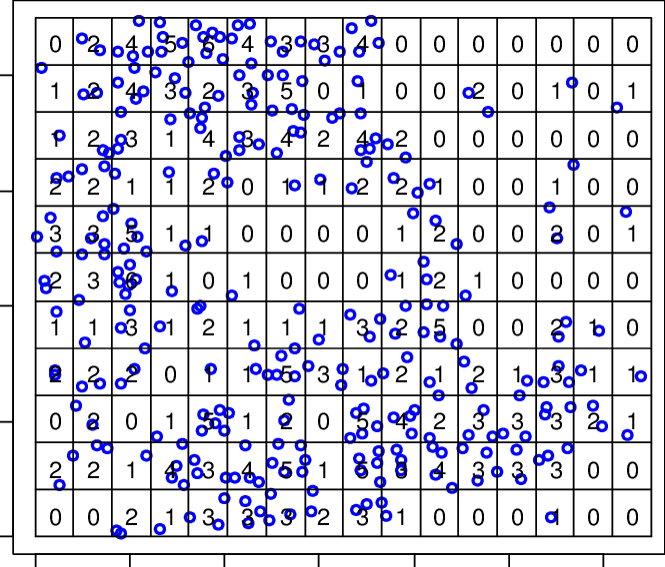
\includegraphics{images/quadrat.png}
\caption{\label{fig:unnamed-chunk-125}Poisson point process}
\end{figure}

In the above figure, we quantify the \emph{spatial intensity} of events by calculating \(\lambda = \frac{n}{area}\). Thus, all of our statistical analysis to date is premised on this idea that the spatial location of points can be interpreted through the lens of a \emph{Poisson} probability distribution. But what if we could calculate the \emph{spatial intensity} more continuously, without the constraint of a specific parametric distribution, and without using the possibly arbitrary boundaries and zoning schemes of areal geographic units such as census tracts, zip codes, or counties?

\emph{Spatial point process} analysis focuses on characterizing patterns derived directly from the location of the points themselves, without arbitrary aggregation. The study of \emph{point process analysis} is broad, but we will focus on one particularly flexible strategy this week: \textbf{kernel density estimation} (KDE). Kernel density estimation has several features making it useful for spatial epidemiology including:

\begin{itemize}
\tightlist
\item
  It is non-parametric, meaning it does not rely on a specific probability distribution (e.g.~Poisson, negative binomial)
\item
  It provides an alternative means for characterizing \emph{local neighbors}. The strategy of the KDE estimators is most similar to \emph{inverse distance weighting}
\item
  It can be used as a primary tool, or can be an intermediate step for creating \emph{spatial weights}, as we will see in \emph{geographically weighted regression}
\item
  While it is really designed for analyzing \emph{points}, we can use it on areal/polygon data as well.
\end{itemize}

\hypertarget{what-is-a-kernel-density-estimator}{%
\subsection{What is a kernel density estimator?}\label{what-is-a-kernel-density-estimator}}

A \emph{kernel} is a function (e.g.~a shape) centered over each point of data. For example, a Gaussian kernel means there is a Gaussian bell-shaped curve centered over each point; the width of the curve is defined by a parameter, \(h\), which stands for the \emph{bandwidth}.

\begin{figure}
\centering
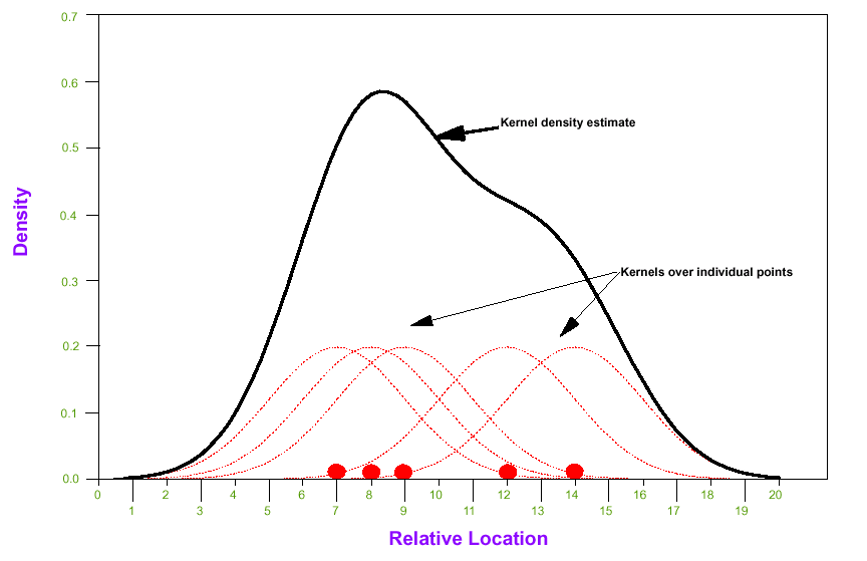
\includegraphics{images/kde2.png}
\caption{\label{fig:unnamed-chunk-126}Kernel density estimator}
\end{figure}

To estimate the \emph{spatial intensity} of points, \(\hat{\lambda}\), we can sum up the area under all of the kernels to estimate an overall \emph{kernel density} at each location. This \emph{kernel density estimate} essentially reports a spatially continuous summary of the \emph{local intensity} of events.

The result is that we can summarize a study region with spatially-referenced point data using a \emph{spatially continuous intensity surface}. The analyst decides on how \emph{smooth} or \emph{bumpy} the surface should be by increasing or decreasing the value of the bandwidth parameter, \(h\). As we will see below, the decision about bandwidth could be made subjectively (e.g.~to produce a visually appealing surface), or by minimizing error or through cross-validation.

\begin{figure}
\centering
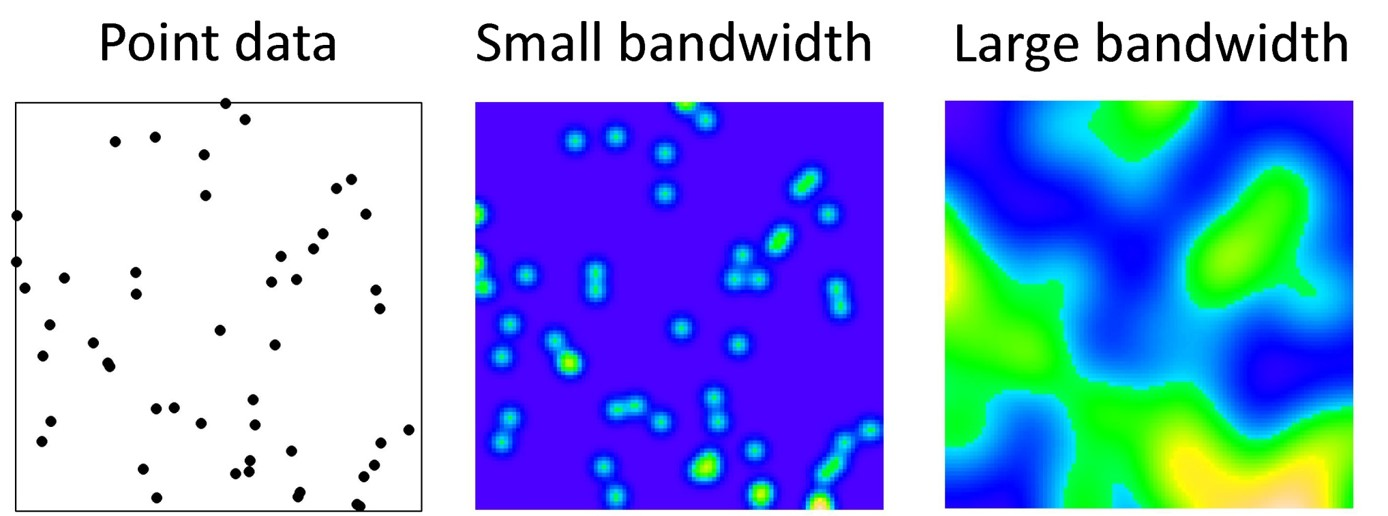
\includegraphics{images/kde3.jpg}
\caption{\label{fig:unnamed-chunk-127}Kernel density smoothing}
\end{figure}

\hypertarget{limitations-in-kernel-density-estimation}{%
\subsection{Limitations in kernel density estimation}\label{limitations-in-kernel-density-estimation}}

There are several features of real data that can limit the accurate estimation of a \emph{true} underlying spatial intensity surface. Here are a few:

\begin{itemize}
\tightlist
\item
  \textbf{Study region and edge effects}: In almost any situation, the data available in a given dataset represents only a subset of the universe of points and events of interest. We can only carry out KDE on available data, and if there are boundaries to where data is collected (e.g.~only within a given state boundary), then the intensity of points near boundaries may be mis-estimated due to missing data. Several of the statistical smoothers below have options to incorporate adjustments for these \emph{edge effects}.
\item
  \textbf{Determining bandwidth}: The choice of the kernel bandwidth is perhaps the most influential decision driving how the final results appear. While occasionally there may be theoretical grounds for \emph{a priori} specification of bandwidth, often the decision is one of \emph{subjective analyst choice} (typically not ideal) or of statistical optimization. In the sections below there is discussion of \emph{fixed} versus \emph{adaptive} bandwidths, as well as some algorithms for selecting values or at least upper or lower bounds.
\end{itemize}

\hypertarget{uses-for-kernel-density-estimation-kde-in-spatial-epidemiology}{%
\subsection{Uses for kernel density estimation (KDE) in spatial epidemiology}\label{uses-for-kernel-density-estimation-kde-in-spatial-epidemiology}}

Because kernel density estimation is the only method we will learn this semester for working with \emph{point data}, it should be clear that this is one major application. However, more generally, KDE has broad applications. Here are some examples of when you might think about using kernel density estimates:

\begin{itemize}
\tightlist
\item
  For producing spatially continuous (typically \emph{raster}) surfaces representing disease risk. This is the application most consistent with disease mapping, where the purpose is to describe spatial heterogeneity in disease \emph{intensity} or risk.
\item
  For summarizing point-referenced resources (e.g.~retail food outlets; health care clinics; toxic emitters; etc) as an \emph{exposure surface}. This strategy is an alternative to calculating custom distances between each event point and every other resource or exposure. Instead, the kernel density surface summarizes the \emph{average exposure} to all resources at any given point in space.
\item
  For smoothing and summarizing data measured at an areal or polygon unit. While KDE is optimized for point data, it is possible to extend it to smoothing any data (exposure, covariate, or health outcome) measured or reported at an ecologic areal unit.
\item
  Building on the extension of KDE to polygons, we can summarize social or economic \emph{exposure surfaces}. This is a useful way to extend socio-economic-cultural measures that might be available at census geography to represent them as not only contained within specific boundaries, but as being explicitly spatially situated.
\end{itemize}

In the next section, we introduce two different uses of kernel density estimation:

\begin{enumerate}
\def\labelenumi{\arabic{enumi}.}
\tightlist
\item
  First is the intensity estimation of spatial point processes consistent with the description above.
\item
  Second, we illustrate the use of kernel density estimators to create \emph{weights} for \emph{geographically-weighted summary statistics}, including the spatially varying mean risk or rate. This strategy can be applied to either \emph{points} or to \emph{polygons}.
\end{enumerate}

\hypertarget{guide-to-the-rest-of-this-section}{%
\subsection{Guide to the rest of this section\ldots{}}\label{guide-to-the-rest-of-this-section}}

There is a lot of content contained in this module. It is worth highlighting some broad distinctions to help you navigate.

\textbf{The first section} focuses on tools using the \passthrough{\lstinline!sparr!} and \passthrough{\lstinline!spatstat!} packages to create kernel density estimates from \emph{point data}. This includes:

\begin{itemize}
\tightlist
\item
  Creating \passthrough{\lstinline!ppp!} objects for \emph{planar point processes}
\item
  Creating \passthrough{\lstinline!owin!} objects to define study regions
\item
  Discussion of several different strategies for selecting a \emph{kernel bandwidth} which dictates smoothing
\item
  Creation of kernel density surfaces of single point processes
\item
  Creation of kernel density \emph{relative risk} surfaces contrasting the ratio of numerator to denominator intensity
\item
  Visualizing the output in several ways.
\end{itemize}

\textbf{The second section} introduces a seemingly quite distinct strategy for incorporating kernel density estimators into spatial epidemiology. It introduces tools for calculating \emph{geographically weighted summary statistics} to characterize spatial heterogeneity. These tools use kernel density estimators to geographically weight observations, and can be applied to \emph{points} or \emph{polygons}. This section includes:

\hypertarget{spatial-analysis-in-epidemiology-kernel-estimation-of-point-processes}{%
\section{Spatial Analysis in Epidemiology: Kernel estimation of point processes}\label{spatial-analysis-in-epidemiology-kernel-estimation-of-point-processes}}

This section has three specific objectives:

\begin{enumerate}
\def\labelenumi{\arabic{enumi}.}
\tightlist
\item
  Introduce a new spatial data class in \passthrough{\lstinline!R!}, \passthrough{\lstinline!ppp!}, which is necessary for executing the kernel estimation functions
\item
  Introduce kernel density estimation of spatial point processes, including selection of fixed bandwidths, and use of adaptive bandwidths
\item
  Introduce spatial \emph{relative risk surfaces}, including estimation of tolerance contours
\end{enumerate}

\hypertarget{preparing-packages-and-data}{%
\subsection{Preparing packages and data}\label{preparing-packages-and-data}}

There are several new packages that will be required for this work:

\begin{lstlisting}[language=R]
library(sparr)         # A package for estimating spatial intensity and relative risk
library(spatstat)      # A package with tools that underly the sparr package
library(maptools)      # This has a helper function for working with ppp class data
library(raster)        # The outputs of these KDE functions will be raster. This package gives us tools for working with rasters
\end{lstlisting}

In addition to those new packages, we will also need the \passthrough{\lstinline!sp!} package. Recall that we have only worked with \passthrough{\lstinline!sf!} class data up until now, although we learned that \passthrough{\lstinline!sp!} was the \emph{older format} for spatial data in \passthrough{\lstinline!R!}. Some packages and functions (including \passthrough{\lstinline!sparr!} and \passthrough{\lstinline!spatstat!}) have not incorporated compatibility with \passthrough{\lstinline!sf!} data, so we will need to convert some particular objects from \passthrough{\lstinline!sf!} to \passthrough{\lstinline!sp!} before moving forward.

The data used in this example, and in the lab, concerns the exact \(x,y\) residential location of all births in Dekalb and Fulton county, including indication of infants who subsequently died within the first year of life.

\begin{quote}
NOTE: These data are simulated based on approximate patterns. This is \textbf{not a representation of actual point data}.
\end{quote}

The spatial point location for births and infant deaths are in two separate files. In addition a polygon file providing the outline for Dekalb and Fulton counties is provided to describe the \emph{study window}.

\begin{lstlisting}[language=R]
# This is points for births in Dekalb/Fulton county
b_point <- st_read('birth_points.gpkg')

# This is points for deaths in Dekalb/Fulton county
d_point <- st_read('death_points.gpkg') 

# This is an outline of Dekalb/Fulton county to be used as a study 'window'
county <- st_read('DekalbFultonWindow.gpkg') %>%
  as('Spatial')
\end{lstlisting}

In the code above, note the us of the function \passthrough{\lstinline!as('Spatial')!} for the object \passthrough{\lstinline!county!}. This is a conversion step, translating the \passthrough{\lstinline!sf!} object to an object of class \passthrough{\lstinline!sp!}. It is only necessary in this particular case for the polygon file representing the \emph{study window} because the functions the create that window expect data of class \passthrough{\lstinline!sp!}. In contrast we can extract the coordinates from an \passthrough{\lstinline!sf!} point object, without a need to convert to \passthrough{\lstinline!sp!} first.

\hypertarget{introducing-a-new-spatial-data-class-ppp}{%
\subsection{\texorpdfstring{Introducing a new spatial data class: \texttt{ppp}}{Introducing a new spatial data class: ppp}}\label{introducing-a-new-spatial-data-class-ppp}}

Much of the statistical methods for spatial point process actually developed out of \emph{ecology}, and the methods are only merging with the other spatial analysis and spatial epidemiology fields in recent years. One consequence of this history, is that the early developers of these methods in \passthrough{\lstinline!R!} defined their own spatial data class called \passthrough{\lstinline!ppp!} for point pattern data in a two-dimensional plane.

To create a \passthrough{\lstinline!ppp!} data object we need, at a minimum, two things: a matrix of \(x,y\) coordinates for event points, and a definition for the \emph{spatial window} or study region. This \emph{window} is necessary because nearly any data set is a sub-sample of the universe of possible \emph{points}, and analysis of point processes requires appreciation for the bounds of sampling. We define the window formally in \passthrough{\lstinline!R!} as an object of class \passthrough{\lstinline!owin!}, and it can be a rectangular bounding box (e.g.~the outline of the available data), or a customized polygon. We will use the outline of Dekalb \& Fulton counties as the customized \emph{spatial window} for the observation of births and infant deaths. Note that the function below to create the \passthrough{\lstinline!owin!} object only works on \passthrough{\lstinline!sp!} class \passthrough{\lstinline!SpatialPolygons!}. That is why we converted the polygon file to class \passthrough{\lstinline!sp!} when we imported (above).

You can see from the summary and the plot what this \passthrough{\lstinline!owin!} object looks like.

\begin{lstlisting}[language=R]
county_owin <- maptools::as.owin.SpatialPolygons(county)
summary(county_owin)
\end{lstlisting}

\begin{lstlisting}
## Window: polygonal boundary
## single connected closed polygon with 698 vertices
## enclosing rectangle: [1026366.3, 1098719.2] x [1220671, 1302019.3] units
##                      (72350 x 81350 units)
## Window area = 2086320000 square units
## Fraction of frame area: 0.354
\end{lstlisting}

\begin{lstlisting}[language=R]
plot(county_owin)
\end{lstlisting}

\includegraphics{EPI563-SpatialEPI_files/figure-latex/unnamed-chunk-132-1.pdf}

\hypertarget{creating-the-ppp-objects}{%
\subsection{\texorpdfstring{Creating the \texttt{ppp} objects}{Creating the ppp objects}}\label{creating-the-ppp-objects}}

Now we will use the function \passthrough{\lstinline!ppp()!} to create objects of class \passthrough{\lstinline!ppp!} for each of the \emph{spatial point} files, \passthrough{\lstinline!b\_point!} (representing locations of all births), and \passthrough{\lstinline!d\_point!} (representing locations of all deaths). Doing so requires definition of the \emph{study window} defined above as the object name \passthrough{\lstinline!countr\_owin!} of class \passthrough{\lstinline!owin!}. Again, the study window delineates what is \emph{in} versus \emph{out} of the study area and demarcates \emph{edges} of the study region. You can look at the help documentation for the function \passthrough{\lstinline!ppp()!} to see the arguments. Note that because the function requires specification of the \(x,y\) locations as two separate vectors, we extract the coordinate values from our \passthrough{\lstinline!sf!} object using \passthrough{\lstinline!st\_coordinates()!}.

\begin{lstlisting}[language=R]
# Create the birth ppp object
b_ppp <- ppp(x = st_coordinates(b_point)[, 1], 
             y = st_coordinates(b_point)[, 2],
             window = county_owin)

# Create the death ppp object
d_ppp <- ppp(x = st_coordinates(d_point)[, 1], 
             y = st_coordinates(d_point)[, 2],
             window = county_owin)
\end{lstlisting}

As you might expect, there are built-in methods (from the \passthrough{\lstinline!spatstat!} package) to summarize and plot \passthrough{\lstinline!ppp!} objects.

\begin{lstlisting}[language=R]
summary(d_ppp)
\end{lstlisting}

\begin{lstlisting}
## Planar point pattern:  701 points
## Average intensity 3.359978e-07 points per square unit
## 
## Coordinates are given to 2 decimal places
## i.e. rounded to the nearest multiple of 0.01 units
## 
## Window: polygonal boundary
## single connected closed polygon with 698 vertices
## enclosing rectangle: [1026366.3, 1098719.2] x [1220671, 1302019.3] units
##                      (72350 x 81350 units)
## Window area = 2086320000 square units
## Fraction of frame area: 0.354
\end{lstlisting}

\begin{lstlisting}[language=R]
plot(d_ppp)
\end{lstlisting}

\includegraphics{EPI563-SpatialEPI_files/figure-latex/unnamed-chunk-134-1.pdf}

The summary includes information about the overall \emph{spatial intensity} (e.g.~events per unit area), as well as the number of points, and the observational window. The plot for \passthrough{\lstinline!d\_ppp!} should look just like a plot of \passthrough{\lstinline!d\_point!} as they both contain the same information. Of note, if you repeat the above code for all of the birth events, \passthrough{\lstinline!b\_point!}, the plot will be less readable because there are over 94,000 births as compared with only 705 deaths!

\hypertarget{bandwidth-selection}{%
\subsection{Bandwidth selection}\label{bandwidth-selection}}

As discussed above, and in lecture, the kernel density estimation requires the analyst to specify a \emph{kernel function} (e.g.~a Gaussian kernel, or a quartic bi-weight kernel), and a \emph{kernel bandwidth}. Of the two, the bandwidth is substantially more impactful on results than choice of kernel function.

As a reminder, the \emph{bandwidth} (sometimes indicated by variable \(h\)) describes the \emph{width} or \emph{radius} of the kernel function, and as a result dictates how \emph{smooth} the resulting intensity surface will be. A small bandwidth will produce a bumpier or rougher surface, whereas a larger bandwidth will result in more smoothing. Relating this to our work in previous weeks, the \emph{bandwidth} is also a representation of \emph{local}. In other words it defines which sets of points will be considered \emph{close} and which are not.

There are two general kinds of bandwidth settings:

\begin{enumerate}
\def\labelenumi{\arabic{enumi}.}
\tightlist
\item
  \textbf{Fixed bandwidths:} A single value if \(h\) designates that the width of the kernel (and thus the resulting smoothness of the estimated intensity surface) is the same for the entire study region. Fixed bandwidths are commonly used, and sensible for a study region with relatively homogenous population at risk. However choosing a single value can be challenging in practice when the density of points varies substantially across the study region, as could be the case when your study region includes a range from very urban to very rural.
\item
  \textbf{Adaptive bandwidths:} As the name implies, this approach changes or \emph{adapts} the size of the kernel density bandwidth according to the density of points (data) in differing sub-areas of the overall study region. The result is relatively more smoothing (larger bandwidth) in areas with sparse point data, and relatively less smoothing (smaller bandwidth) in areas with more point density.
\end{enumerate}

While not exactly the same, the specification of bandwidth is conceptually similar to the varying approaches to defining spatial neighbors of polygons. The \emph{fixed bandwidth} is similar to a \emph{fixed-distance buffer} or \emph{inverse-distance} definition, whereas the \emph{adaptive bandwidth} is similar in some ways to a \emph{k-nearest neighbors} in that the distance adjusts according to density of units.

\hypertarget{fixed-bandwidth-methods}{%
\subsubsection{Fixed bandwidth methods}\label{fixed-bandwidth-methods}}

If you prefer a \emph{fixed bandwidth}, the first challenge is choosing what it should be. One option for selecting a \emph{fixed bandwidth} is to incorporate theory or prior knowledge about the process of interest. For instance, if you are trying to understand whether the prevalence of diabetes is related to local food environment in an urban area, you might want a bandwidth which helps illuminate differences in diabetes \emph{intensity} at a scale consistent with the food environment. For instance a bandwidth of \emph{1-mile} might be more reasonable in urban areas than one of \emph{50-miles}, as the latter would likely smooth away all of the local variation of interest.

However, it is not uncommon that theory or prior knowledge are insufficient to make a clear choice, or that data sparsity mandates an alternate approach driven by concern for stable estimates. The package \passthrough{\lstinline!sparr!} has several functions designed to use primarily statistical optimization for estimating an \emph{`optimum'} bandwidth. We will introduce two commonly used statistical bandwidth selection optimizers:

\begin{enumerate}
\def\labelenumi{\arabic{enumi}.}
\tightlist
\item
  \textbf{Cross-validation:} this approach divides the data into subsets, using one subset to choose a bandwidth, and comparing the performance on other subsets. The goal is to find a value that works \emph{`best'} (e.g.~optimize a statistical parameter across multiple iterations). The approach is computationally intensive for large datasets, and in some instances will result in a bandwidth value that is \emph{too small}. As discussed in note below, cross-validation can result in \emph{too small} bandwidth estimation.
\item
  \textbf{Oversmoothing:} this is an alternate approach that aims to identify the maximum amount of smoothing necessary for minimizing statistical error. By definition it is a \emph{maximum} value rather than an \emph{ideal} or \emph{optimal} value, but can be useful in setting bounds.
\end{enumerate}

\begin{rmdnote}
The \passthrough{\lstinline!sparr!} package actually three \emph{cross-validation} approaches to estimation: \passthrough{\lstinline!LCSV.density!} (least squares cross validated); \passthrough{\lstinline!LIK.density!} (likelihood cross-validated); and \passthrough{\lstinline!SLIK.adapt!} (described as an experimental likelihood cross-validation for adaptive). Each is `optimizing' a different thing\ldots the \passthrough{\lstinline!LSCV.density!} minimizes an unbiased estimate of the mean integrated squared error (MISE) whereas \passthrough{\lstinline!LIK.density!} maximizes cross-validated leave one out average of the log-likelihood of the density estimate.
If you look at the help documentation for these you will see (near the bottom) a prominent warning message. It reports that ``CV for bandwidth selection is notoriously unstable in practice and has a tendency to produced rather small bandwidths\ldots{}''\\
\end{rmdnote}

\hypertarget{cross-validation-with-lik.density}{%
\subsubsection{\texorpdfstring{Cross-validation with \texttt{LIK.density()}}{Cross-validation with LIK.density()}}\label{cross-validation-with-lik.density}}

\passthrough{\lstinline!LIK.density()!} uses likelihood estimation of cross-validation optimal bandwidth. For the \emph{death} dataset, \passthrough{\lstinline!d\_ppp!}, it runs in just a few seconds. However it took \textgreater{} 5 minutes to produce a value on the much larger \emph{births} dataset, \passthrough{\lstinline!b\_ppp!}. This code lets you try it to see what it produces:

\begin{lstlisting}[language=R]
h_LIK_d <- LIK.density(d_ppp)
\end{lstlisting}

\begin{lstlisting}
## Searching for optimal h in [27.463186212964, 12058.8149770359]...Done.
\end{lstlisting}

\begin{lstlisting}[language=R]
print(h_LIK_d)
\end{lstlisting}

\begin{lstlisting}
## [1] 1613.661
\end{lstlisting}

If you examine the object returned (\passthrough{\lstinline!h\_LIK\_d!}), you'll see it is just a single number. This is the value of \(h\), or the optimized bandwidth. It is, in other words, the radius of the 2-dimensional kernel density function in the units of the data, which is \emph{meters} in this case (e.g.~the original data were \emph{Albers Equal Area} projected). So this means that the optimum kernel will have a radius of just over 1.5 kilometers.

\hypertarget{oversmoothing-algorithm-with-function-os}{%
\subsubsection{\texorpdfstring{Oversmoothing algorithm with function \texttt{OS()}}{Oversmoothing algorithm with function OS()}}\label{oversmoothing-algorithm-with-function-os}}

This approach is much less computationally intense, and thus feasible for both of our spatial point processes. As we will see below, we can use the value returned from \passthrough{\lstinline!OS()!} as a \emph{pilot value} for \emph{adaptive bandwidth} estimation. In other words it provides a kind of reference or starting point for the adaptation process.

\begin{lstlisting}[language=R]
h_os_d <- OS(d_ppp)
h_os_b <- OS(b_ppp)

print(h_os_d)
\end{lstlisting}

\begin{lstlisting}
## [1] 4257.798
\end{lstlisting}

\begin{lstlisting}[language=R]
print(h_os_b)
\end{lstlisting}

\begin{lstlisting}
## [1] 1897.371
\end{lstlisting}

Note that the \emph{birth} data have a smaller optimal bandwidth (\passthrough{\lstinline!h\_os\_b!}) because there are more points. More points means more information is available for more granular smoothing, whereas the relatively more sparse \emph{death} data have a larger over smoothing bandwidth (\passthrough{\lstinline!h\_os\_d!}).

\hypertarget{selecting-a-common-bandwidth-for-both-numerator-and-denominator}{%
\subsubsection{Selecting a common bandwidth for both numerator and denominator}\label{selecting-a-common-bandwidth-for-both-numerator-and-denominator}}

One challenge in bandwidth selection is that we typically have two related spatial point processes (e.g.~the numerator, death events; and the denominator, birth events). Therefore we don't want only a single KDE, but instead we will need to consider a numerator representing the spatial intensity of deaths, and a denominator representing the spatial intensity of all live births at risk. This raises the question of whether there should be a common bandwidth for both, or whether each should be optimized separately.

While there may be only minor differences in the \emph{absolute intensity} under different bandwidths in a single point process, taking the ratio of two intensity surfaces can exaggerate small differences to be quite large. There are functions for estimating a single, joint, optimum for the bandwidth. The function \passthrough{\lstinline!LSCV.risk()!} does just what the \passthrough{\lstinline!LIK.density()!} above did, but with two spatial point processes. The code example is below, but like the previous example, the cross-validation approach to the birth data set takes an excessive amount of time (at least for this exercise).

\begin{lstlisting}[language=R]
#h_LSCV_risk <- LSCV.risk(d_ppp, b_ppp)
\end{lstlisting}

\hypertarget{adaptive-bandwidth-methods}{%
\subsubsection{Adaptive bandwidth methods}\label{adaptive-bandwidth-methods}}

Adaptive methods are specified \emph{at the time of kernel density estimation}. While the bandwidth is not constant, but instead \emph{adaptive}, we usually still need to specify a \emph{pilot bandwidth}, which is a reference point from which adaptation occurs. As mentioned above, the \emph{oversmoothing} approach from \passthrough{\lstinline!OS()!} can be used as a pilot value.

\hypertarget{estimating-kernel-density-surfaces}{%
\subsection{Estimating Kernel Density surfaces}\label{estimating-kernel-density-surfaces}}

We now turn to the actual estimation of kernel density approximations of the underlying \emph{spatial intensity} of disease. The approach in this lab is to first illustrate how to estimate separate densities for each point process (e.g.~of \emph{deaths} and of \emph{births}), and then to demonstrate two strategies for creating \emph{spatial relative risk surfaces}, which is generally the target output for spatial epidemiologists.

Of note, this discussion will demonstrate use of both \emph{fixed} and \emph{adaptive} bandwidths. In general adaptive bandwidths may be the most practical approach \emph{in the absence of theoretical or empirical preference} otherwise. However there are instances where \emph{fixed bandwidths} (either theoretically informed, or as derived from CV or oversmoothing algorithms) are desired, and thus seeing both in action is useful.

\hypertarget{bivariate.density-for-kde-of-single-point-process}{%
\subsubsection{\texorpdfstring{\texttt{bivariate.density()} for KDE of single point process}{bivariate.density() for KDE of single point process}}\label{bivariate.density-for-kde-of-single-point-process}}

There are actually several \passthrough{\lstinline!R!} packages that accomplish kernel density estimation, but one that is particularly useful for spatial epidemiology (where the kernel density estimator must be 2-dimensional and not just 1-dimensional) is the \passthrough{\lstinline!sparr!} package, which stands for \emph{Spatial and Spatiotemporal Relative Risk}.

The \passthrough{\lstinline!sparr!} function \passthrough{\lstinline!bivariate.density()!} is a flexible and useful tool for carrying out KDE with either \emph{fixed} or \emph{adaptive} bandwidths. There are many arguments for \passthrough{\lstinline!bivariate.density()!} (see help documentation), but there are several worth specifically highlighting here.

\begin{longtable}[]{@{}ll@{}}
\toprule
\begin{minipage}[b]{0.16\columnwidth}\raggedright
Function\strut
\end{minipage} & \begin{minipage}[b]{0.78\columnwidth}\raggedright
Description\strut
\end{minipage}\tabularnewline
\midrule
\endhead
\begin{minipage}[t]{0.16\columnwidth}\raggedright
\textbf{\passthrough{\lstinline!pp!}}\strut
\end{minipage} & \begin{minipage}[t]{0.78\columnwidth}\raggedright
This first argument expects a \emph{single} point process object of class \passthrough{\lstinline!ppp!}. We will use either \passthrough{\lstinline!d\_ppp!} or \passthrough{\lstinline!b\_ppp!}\strut
\end{minipage}\tabularnewline
\begin{minipage}[t]{0.16\columnwidth}\raggedright
\textbf{\passthrough{\lstinline!h0!}}\strut
\end{minipage} & \begin{minipage}[t]{0.78\columnwidth}\raggedright
This argument specifies the \emph{global fixed} bandwidth, if desired. This could be a theoretically-informed value, or derived from an optimization algorithm (e.g.~see above)\strut
\end{minipage}\tabularnewline
\begin{minipage}[t]{0.16\columnwidth}\raggedright
\textbf{\passthrough{\lstinline!hp!}}\strut
\end{minipage} & \begin{minipage}[t]{0.78\columnwidth}\raggedright
If conducting \emph{adaptive bandwidth} estimation, a single \emph{pilot bandwidth} is still required, and this is where to specify it.\strut
\end{minipage}\tabularnewline
\begin{minipage}[t]{0.16\columnwidth}\raggedright
\textbf{\passthrough{\lstinline!adapt!}}\strut
\end{minipage} & \begin{minipage}[t]{0.78\columnwidth}\raggedright
This logical argument is \passthrough{\lstinline!FALSE!} by default, but set to \passthrough{\lstinline!TRUE!} if you want adaptive bandwidth estimation\strut
\end{minipage}\tabularnewline
\begin{minipage}[t]{0.16\columnwidth}\raggedright
\textbf{\passthrough{\lstinline!edge!}}\strut
\end{minipage} & \begin{minipage}[t]{0.78\columnwidth}\raggedright
Because a given dataset is invariably a subset of the real world, there are likely \emph{edges} where there is an artificially abrupt cessation of information. The result is a potentially biased intensity estimation at the study region edges. However there are correction factors. We will choose the \passthrough{\lstinline!edge = 'diggle'!} specification here\strut
\end{minipage}\tabularnewline
\begin{minipage}[t]{0.16\columnwidth}\raggedright
\textbf{\passthrough{\lstinline!intensity!}}\strut
\end{minipage} & \begin{minipage}[t]{0.78\columnwidth}\raggedright
Up until now we have used the words \textbf{intensity} and \textbf{density} as if they are synonymous for point process parameter, but that is not the case. \textbf{Intensity} is the \emph{average number of points per unit area}. The \textbf{density} is proportionate to the \emph{intensity}, but scaled so that all values in the study region \emph{sum to 1}. In other words a \textbf{density surface} is a proper probability density function. By default, \passthrough{\lstinline!intensity = FALSE!} which means that by default \passthrough{\lstinline!bivariate.density()!} produces a \emph{density surface}. If you want \emph{intensity}, set \passthrough{\lstinline!intensity = TRUE!}.\strut
\end{minipage}\tabularnewline
\bottomrule
\end{longtable}

\hypertarget{fixed-bandwidth-kde-with-bivariate.density}{%
\subsubsection{\texorpdfstring{Fixed bandwidth KDE with \texttt{bivariate.density()}}{Fixed bandwidth KDE with bivariate.density()}}\label{fixed-bandwidth-kde-with-bivariate.density}}

First, let's try a basic version that uses the \emph{oversmooth} estimate for each point process.

\begin{lstlisting}[language=R]
death_kde <- bivariate.density(pp = d_ppp, h0 = h_os_d, edge = 'diggle')
birth_kde <- bivariate.density(pp = b_ppp, h0 = h_os_b, edge = 'diggle')
\end{lstlisting}

You can explore the objects produced by the function call. For instance, they are \passthrough{\lstinline!list!} objects, with named sub-elements:

\begin{lstlisting}[language=R]
summary(birth_kde)
\end{lstlisting}

\begin{lstlisting}
## Bivariate Kernel Density/Intensity Estimate
## 
## Bandwidth
##   Fixed smoothing with h0 = 1897.371 units (to 4 d.p.)
## 
## No. of observations
##   94373 
## 
## Spatial bound
##   Type: polygonal
##   2D enclosure: [1026366, 1098719] x [1220671, 1302019]
## 
## Evaluation
##   128 x 128 rectangular grid
##   5808 grid cells out of 16384 fall inside study region
##   Density/intensity range [6.313906e-14, 1.585466e-09]
\end{lstlisting}

\begin{lstlisting}[language=R]
names(birth_kde)
\end{lstlisting}

\begin{lstlisting}
## [1] "z"         "h0"        "hp"        "h"         "him"       "q"        
## [7] "gamma"     "geometric" "pp"
\end{lstlisting}

There is also some plotting functionality built into the \passthrough{\lstinline!sparr!} package that allows us to quickly visualize the resulting density plot.

\begin{lstlisting}[language=R]
par(mfrow = c(1, 2))
plot(birth_kde, main = 'Birth density')
plot(death_kde, main = 'Death density')
\end{lstlisting}

\includegraphics{EPI563-SpatialEPI_files/figure-latex/unnamed-chunk-141-1.pdf}

\begin{lstlisting}[language=R]
par(mfrow = c(1,1))
\end{lstlisting}

\hypertarget{adaptive-bandwidth-kde-with-bivariate.density}{%
\subsubsection{\texorpdfstring{Adaptive bandwidth KDE with \texttt{bivariate.density()}}{Adaptive bandwidth KDE with bivariate.density()}}\label{adaptive-bandwidth-kde-with-bivariate.density}}

As discussed above, an alternative to a single \emph{fixed bandwidth}, is implementation of an algorithm that changes (\emph{adapts}) the bandwidth across the study region in response to the density or sparseness of the data. This approach still requires specification of a \emph{global} bandwidth, and the adaptation is a multiplier making the global smaller or larger as needed. In this code we use the argument \passthrough{\lstinline!h0 =!} to specify a \emph{pilot bandwidth}. Because \emph{adaptive bandwidth KDE} requires adjustment across the study region, you will notice that these functions take longer than the \emph{fixed bandwidth} above, especially the large birth point process.

\begin{lstlisting}[language=R]
death_kde_adapt <- bivariate.density(d_ppp, 
                                     h0 = h_os_d, 
                                     edge = 'diggle', 
                                     adapt = TRUE,
                                     verbose = FALSE)
birth_kde_adapt <- bivariate.density(b_ppp, 
                                     h0 = h_os_b, 
                                     edge = 'diggle',
                                     adapt = TRUE,
                                     verbose = FALSE)
par(mfrow = c(1, 2))
plot(birth_kde_adapt, main = 'Birth density\n(adaptive h)')
plot(death_kde_adapt, main = 'Death density\n(adaptive h)')
\end{lstlisting}

\includegraphics{EPI563-SpatialEPI_files/figure-latex/unnamed-chunk-142-1.pdf}

\begin{lstlisting}[language=R]
par(mfrow = c(1,1))
\end{lstlisting}

Does this result from the \emph{adaptive} bandwidth look different from the \emph{fixed} bandwidth? \emph{Not really}. The reason is because the units of measurement (intensity) are so small that differences are not apparent. However the differences become more apparent when we take the ratio of the two surfaces, which we will do below.

\hypertarget{plotting-kde-estimates-with-tmap}{%
\subsubsection{\texorpdfstring{Plotting KDE estimates with \texttt{tmap}}{Plotting KDE estimates with tmap}}\label{plotting-kde-estimates-with-tmap}}

It is handy that the \passthrough{\lstinline!sparr!} package has some built-in plotting functionality to quickly visualize the results. However you may want to have more control over the plotting, for instance in \passthrough{\lstinline!tmap!} or even in \passthrough{\lstinline!ggplot2!}.

If you recall the named elements in the \passthrough{\lstinline!list!} object returned by \passthrough{\lstinline!bivariate.density()!}, the first is called \passthrough{\lstinline!z!}, and this is the density surface itself.

\begin{lstlisting}[language=R]
class(birth_kde$z)
\end{lstlisting}

\begin{lstlisting}
## [1] "im"
\end{lstlisting}

The class of this object is \passthrough{\lstinline!im!} for \emph{image}. However for almost any spatial plotting or operation outside of \passthrough{\lstinline!sparr!} and \passthrough{\lstinline!spatstat!}, we want this data in the \passthrough{\lstinline!raster!} class rather than this \passthrough{\lstinline!im!} format (fundamentally the data \emph{is} a raster model, but the data structure in \passthrough{\lstinline!R!} is not quite the same as the data structure of class \passthrough{\lstinline!raster!}). We can convert \passthrough{\lstinline!im!} to \passthrough{\lstinline!raster!} class like this:

\begin{lstlisting}[language=R]
death_kde_raster <- raster(death_kde_adapt$z,
                           crs = "+init=epsg:5070")
birth_kde_raster <- raster(birth_kde_adapt$z,
                           crs = "+init=epsg:5070")
\end{lstlisting}

NOtice in the code above the specification of \passthrough{\lstinline!crs = "+init=epsg:5070"!}. The \passthrough{\lstinline!im!} object lost all information about the original \emph{coordinate reference system} (CRS) or \emph{projection}. However, we need our raster object to have this CRS information to plot properly in \passthrough{\lstinline!tmap!}. We know that the original point data were \emph{projected} in \emph{Albers Equal Area}, specificlly with \emph{EPSG code} of 5070. So we re-define that when creating the rasters above.

Now we can plot these in \passthrough{\lstinline!tmap!}:

\begin{lstlisting}[language=R]
# Create map of death surface
m1 <- tm_shape(death_kde_raster) + 
  tm_raster(palette = 'BuPu',
            style = 'quantile',
            n = 9,
            title = 'Death density') +
  tm_layout(legend.format = list(scientific = T))

# Create map of birth surface
m2 <- tm_shape(birth_kde_raster) +
  tm_raster(palette = 'BuPu',
            style = 'quantile',
            n = 9,
            title = 'Birth density') +
  tm_layout(legend.format = list(scientific = T))

# plot 2-panel arrangment
tmap_arrange(m1, m2)
\end{lstlisting}

\includegraphics{EPI563-SpatialEPI_files/figure-latex/unnamed-chunk-145-1.pdf}
Notice how the resulting maps look a little \emph{pixely}. There are two reasons contributing this. First, the code above specified the colors in quantiles in order to get a range despite possibly skewed values. But you could try re-plotting the above plots setting \passthrough{\lstinline!style = 'cont'!} for \emph{continuous} color palette, and comment out the \passthrough{\lstinline!n=9!}. You will see that this produces a much \emph{smoother} looking plot. The difference between the plots with \passthrough{\lstinline!style = 'cont'!} and \passthrough{\lstinline!style = 'quantile'!} is the gradation of color in the intermediate levels of intensity.

But the other reason for the pixelation is because the original call to \passthrough{\lstinline!bivariate.density()!} used the default output resolution of 128 x 128 grid cells. This was done for computational efficiency. However, note that if you want a higher-resolution surface (e.g.~for publication, presentation), you can increase by specifying \passthrough{\lstinline!resolution =!} in the creation of the KDE surface in the original call to \passthrough{\lstinline!bivariate.density()!}.

\hypertarget{creating-relative-risk-surface-manually}{%
\subsection{Creating relative risk surface manually}\label{creating-relative-risk-surface-manually}}

Up until now, we have only created the KDE surface for the \emph{death} and \emph{birth} points separately. But for epidemiology, we rarely care about numerator and denominator separately! So how do we put these two together into a more informative disease map?

\emph{Raster algebra} is a term for arithmetic and algebraic manipulation of raster grids. Recall that a \emph{raster} data set is simply a array of numbers. The numbered value of each grid-point represents the mean density or intensity of points per unit-area, and is mapped as color to make the plot. Because it is simply a matrix of numbers, we can take two rasters of the same resolution and study area and add, subtract, multiply, log-transform, or otherwise operate on them arithmetically.

For instance to manually create \emph{spatial relative risk surface} we simply take the ratio of two KDE density surfaces. The result is a relative measure akin to the SMR: it quantifies the relative deviation of each area from an overall average value. So values below 1 are areas with \emph{lower than average risk}, meaning that the intensity of \emph{deaths} is less than the intensity of \emph{live births}, and values above 1 have \emph{higher than average risk} (the intensity of \emph{deaths} is greater than the intensity of \emph{live births}).

\begin{rmdnote}
For interpretting the \emph{ratio of two kernel surfaces} take care to distinguish between the \textbf{spatial intensity} (number of point events per unit area; the value integrates or sums to the total number of points across the study region) versus the \textbf{spatial density} (probability of a point event occuring at this location, conditional on total number of points; integrates to 1 across the study region). The distinction is important. The default output of \passthrough{\lstinline!bivariate.density()!} function is a \emph{spatial density surface}. The ratio of two density (probability) surfaces will take the value of 1.0 when the probability of a death at that location is proportionate to the probability of a birth at that location. In contrast the ratio of two intensity surfaces is interpretted as an absolute measure (e.g.~risk, rate, prevalence) ranging from zero to 1. If you choose \passthrough{\lstinline!intensity = TRUE!} when specifying the \passthrough{\lstinline!bivariate.density()!} function you will get the intensity rather than (default) density surface.
\end{rmdnote}

In the \passthrough{\lstinline!tmap!} call I \emph{flipped} the color ramp by using the negative sign in front of the name of the ramp. I also specified a continuous style rather than discrete (e.g.~\passthrough{\lstinline!quantile!}), and specified some legend breaks.

\begin{lstlisting}[language=R]
# Create risk surface as ratio of death density to birth density
risk <- death_kde_raster / birth_kde_raster

# Map it...
tm_shape(risk) + 
  tm_raster(palette = '-RdYlGn',
            style = 'cont',
            breaks = c(0.1, 0.6, 0.9,   1.1, 2, 4.9),
            title = 'IMR SMR') 
\end{lstlisting}

\includegraphics{EPI563-SpatialEPI_files/figure-latex/unnamed-chunk-147-1.pdf}

Now we can more clearly see regions of \emph{higher risk} and \emph{lower risk} of infant mortality!

\hypertarget{creating-relative-risk-surface-with-risk-function}{%
\subsection{\texorpdfstring{Creating relative risk surface with \texttt{risk()} function}{Creating relative risk surface with risk() function}}\label{creating-relative-risk-surface-with-risk-function}}

The preceding \emph{manual} approach created two separate kernel density surfaces, and then manually relied on raster algebra to create the spatial relative risk surface. This is useful to know because you may use KDE in other setting where you only work with a single spatial point process (e.g.~imagine that instead of estimating disease intensity, you wish to estimate an \emph{exposure} density surface).

However, the \passthrough{\lstinline!sparr!} package provides a shortcut for estimation of spatial relative risk surfaces in the function \passthrough{\lstinline!risk()!}. It takes a numerator and denominator \passthrough{\lstinline!ppp!} object as arguments and calculates the spatial relative risk surface automatically.

As a demonstration of comparing four arbitrary, fixed bandwidths for the purposes of data exploration, below we estimate four distinct spatial relative risk surfaces, as well as one adaptive KDE. In each case notice the first two arguments are the numerator and denominator \passthrough{\lstinline!ppp!} object. The next argument is a pre-specified fixed bandwidth (e.g.~1000, 2000, 4000, and 8000 meters).

This function also illustrates another \emph{feature} which allows us to quantify statistical precision by creating \emph{tolerance contours}. Tolerance contours are simply lines which encircle regions that are statistically significant below a given threshold. The argument \passthrough{\lstinline!tolerate = T!} tells the function to estimate \emph{asymptotic} p-values testing the null hypothesis that the local relative risk of death is equal across the study region.

By default, the function estimates the \emph{log relative risk}, which is a helpful reminder that the \emph{relative risk} is asymmetric. However, we understand ratio measures, and will be careful to plot the results appropriately. For that reason, I set \passthrough{\lstinline!log = FALSE!}, although obviously you could omit that and keep everything on the \passthrough{\lstinline!log!} scale.

\textbf{NOTE:} The \emph{fixed bandwidth} \passthrough{\lstinline!risk()!} functions will run quickly, but once again, the \emph{adaptive bandwidth} is more computationally intensive, and will take longer.

\begin{lstlisting}[language=R]
imr1000 <- risk(d_ppp, b_ppp, h0 = 1000, 
            tolerate = T,
            verbose = F, 
            log = F,
            edge = 'diggle')

imr2000 <- risk(d_ppp, b_ppp, h0 = 2000, 
            tolerate = T,
            log = F,
            edge = 'diggle',
            verbose = F)

imr4000 <- risk(d_ppp, b_ppp, h0 = 4000, 
            tolerate = T,
            log = F,
            edge = 'diggle',
            verbose = F)

imr8000 <- risk(d_ppp, b_ppp, h0 = 8000, 
            tolerate = T,
            log = F,
            edge = 'diggle',
            verbose = F)

imradapt <- risk(d_ppp, b_ppp, 
                 h0 = h_os_d, 
                 adapt = T, 
                 tolerate = T,
                 log = F,
                 edge = 'diggle',
                 verbose = F)
\end{lstlisting}

Examine the contents of one of these objects. The summary show us the range of the estimated risk, the resolution of the evaluation grid, and the number of points evaluated.

\begin{lstlisting}[language=R]
summary(imr1000)
\end{lstlisting}

\begin{lstlisting}
## Log-Relative Risk Function.
## 
## Estimated risk range [-8.216873e-14, 11.05946]
## 
## --Numerator (case) density--
## Bivariate Kernel Density/Intensity Estimate
## 
## Bandwidth
##   Fixed smoothing with h0 = 1000 units (to 4 d.p.)
## 
## No. of observations
##   701 
## 
## Spatial bound
##   Type: polygonal
##   2D enclosure: [1026366, 1098719] x [1220671, 1302019]
## 
## Evaluation
##   128 x 128 rectangular grid
##   5808 grid cells out of 16384 fall inside study region
##   Density/intensity range [-1.82875e-25, 2.78467e-09]
## 
## --Denominator (control) density--
## Bivariate Kernel Density/Intensity Estimate
## 
## Bandwidth
##   Fixed smoothing with h0 = 1000 units (to 4 d.p.)
## 
## No. of observations
##   94373 
## 
## Spatial bound
##   Type: polygonal
##   2D enclosure: [1026366, 1098719] x [1220671, 1302019]
## 
## Evaluation
##   128 x 128 rectangular grid
##   5808 grid cells out of 16384 fall inside study region
##   Density/intensity range [2.143127e-16, 2.383589e-09]
\end{lstlisting}

\begin{lstlisting}[language=R]
names(imr1000)
\end{lstlisting}

\begin{lstlisting}
## [1] "rr" "f"  "g"  "P"
\end{lstlisting}

\begin{rmdcaution}
\textbf{BEWARE}: You can see that the range of the estimated risk is \([-8.216873e-14, 11.05946]\). The lower bound is in practical terms zero (e.g.~it is very, very small), but counter-intuitively it is also \emph{negative}! How could we estimated \emph{negative risk}? The answer seems to be related to the Diggle edge correction. For example if you substitute \passthrough{\lstinline!edge = 'uniform'!} the anomaly goes away. This is likely because edge correction (which in the big picture is a valuable strategy) reweights regions and may result in specific location estimates that become negative.
\end{rmdcaution}

Once again, we can use built-in plotting functionality from \passthrough{\lstinline!sparr!} to produce maps of the \emph{spatial relative risk surface} and the tolerance contours. (NOTE: the default legend works best for \emph{log relative risk}, but doesn't behave well for the \emph{relative risk} because it treats the distance from 0 to 1 as the same as the distance from 1 to 2, or 4 to 5).

\begin{lstlisting}[language=R]
par(mar = c(1,1,1,1))
par(mfrow = c(3,2))
plot(imr1000)
plot(imr2000)
plot(imr4000)
plot(imr8000)
plot(imradapt)
par(mfrow = c(1,1))
\end{lstlisting}

\includegraphics{EPI563-SpatialEPI_files/figure-latex/unnamed-chunk-151-1.pdf}

While the code above plots these side-by-side, you might find it easier to plot them one at a time and zoom in closer. Notice the contour lines for \(p<0.05\). Also notice how the risk surface becomes smoother as the fixed bandwidth transitions from \(1km\) to \(8km\). Finally, notice how the \emph{adaptive} bandwidth is consistent with the other maps, but seems to balance the detail between the 2000 meter and 4000 meter definitions.

\hypertarget{using-functions-to-map-rr-with-tmap}{%
\subsection{\texorpdfstring{Using functions to map RR with \texttt{tmap}}{Using functions to map RR with tmap}}\label{using-functions-to-map-rr-with-tmap}}

When we begin plotting several maps, the conversion from the \passthrough{\lstinline!im!} to \passthrough{\lstinline!raster!} and the code for producing map panels can feel cumbersome. While the following section is not required, it is a demonstration of how you can write simple custom functions in \passthrough{\lstinline!R!} to speed up repetitive tasks.

A function in \passthrough{\lstinline!R!} is like a macro in SAS; it is simply a set of instructions that accepts \emph{arguments} (inputs), carries out some action on those inputs, and then \emph{returns} some output.

This is a function that accepts a single \emph{argument}, labeled simply \passthrough{\lstinline!x!} here. The expectation is that \passthrough{\lstinline!x!} should be the output of the above \passthrough{\lstinline!risk()!} function. Notice how the function first extracts the spatial relative risk surface (e.g.~\passthrough{\lstinline!x$rr!}), and then assigns the appropriate projection (it got stripped off some where along the way).

Then the function extracts the \emph{probability map} which is the set of pixel-specific p-values. The \passthrough{\lstinline!rasterToContour()!} function takes this raster and creates contour lines with the specified levels corresponding to a 95\% tolerance contour. Finally, the use of the \passthrough{\lstinline!return()!} tells what should be returned when the function is called.

Once you write a function, it need only be loaded once in a given session; afterwords you can \emph{call} it by using \passthrough{\lstinline!prepRaster(x = my\_risk\_object)!}.

\begin{lstlisting}[language=R]
### --- prepRaster() function --- ###
prepRaster <- function(x){
  rr <- raster(x$rr,
               crs = "+init=epsg:5070")

  p_raster <- raster(x$P,
               crs = "+init=epsg:5070")
  plines <- rasterToContour(p_raster, levels = c(0.025,  0.975))
  
  return(list(rr=rr,plines=plines))
} ## END prepRaster() ##
\end{lstlisting}

While we're on a roll, we could also write a function for producing a \passthrough{\lstinline!tmap!} panel:

\begin{lstlisting}[language=R]
### --- make_map() function to create panel maps --- ###
make_map <- function(x, bw){
  mtitle <- paste('IMR - ', bw, ' smooth', sep = '')
  tm_shape(x$rr) +
  tm_raster(palette = '-RdYlGn',
            style = 'cont',
            breaks = c(0.1, 0.6, 0.9,   1.1, 2, 4.9),
            midpoint = NA,
            title = 'IMR SMR') +
  tm_shape(x$plines) +
  tm_lines(col = 'level',
           legend.col.show = F) + 
  tm_layout(main.title = mtitle,
            legend.format = list(digits = 1)) 
} ## END make_map() function ##
\end{lstlisting}

The result of this work is that we can easily (and more compactly), map the four fixed-bandwidth spatial relative risk surfaces.

\begin{lstlisting}[language=R]
# First convert to raster and extract p-value contours
rr_1000 <- prepRaster(imr1000)
rr_2000 <- prepRaster(imr2000)
rr_4000 <- prepRaster(imr4000)
rr_8000 <- prepRaster(imr8000)
rr_adapt <- prepRaster(imradapt)

# Then produce map panels
m1000 <- make_map(rr_1000, '1 km')
m2000 <- make_map(rr_2000, '2 km')
m4000 <- make_map(rr_4000, '4 km')
m8000 <- make_map(rr_8000, '8 km')
mapadapt <- make_map(rr_adapt, 'adaptive')

tmap_arrange(m1000, m2000, m4000, m8000,mapadapt, ncol = 2)
\end{lstlisting}

\includegraphics{EPI563-SpatialEPI_files/figure-latex/unnamed-chunk-154-1.pdf}

\hypertarget{gwss}{%
\section{Spatial Analysis in Epidemiology: Kernel estimation of areal data}\label{gwss}}

In the preceding section we saw how to use KDE for estimating a smooth \emph{spatial intensity surface} from a spatial point process. In this section we introduce \emph{geographically-weighted} statistics that are extendable to areal units and not only points. There were three key features about the use of KDE from the preceding section that we will extend on here:

\begin{enumerate}
\def\labelenumi{\arabic{enumi}.}
\tightlist
\item
  \emph{KDE are not only for points} - while the whole notion of the kernel density estimation process is indeed connected to the \(x,y\) point location, this does not mean we cannot take advantage of the non-parametric smoothing for other kinds of data, such as polygons. Typically the centroid (geometric center) of a polygon is used as the stand-in for point when KDE is done with polygons.
\item
  \emph{KDE is not only for binary values} - a spatial point process is by definition the a description of the location of discrete points representing a discrete state. For instance in section above, we visualized the spatial intensity surface of infant deaths, and separately the surface of live births. But what if we want to measure a \emph{continuous value} rather than a discrete, binary state at spatial locations? The mechanics of KDE can still be helpful!
\item
  \emph{KDE is a kind of spatial weighting procedure} - this was true in Part A as well\ldots the \emph{spatial intensity} is essentially the spatially-weighted number of points surrounding an index location divided by the area under the kernel function. In this lab the primary use of the kernel function is to produce weights for calculating weighted-statistics including \emph{mean}, \emph{median}, etc of any quantity that is measured.
\end{enumerate}

This lab introduces a function in the package \passthrough{\lstinline!GWmodel!} (e.g.~\emph{geographically weighted models}) that is very useful for exploratory spatial data analysis. The function \passthrough{\lstinline!gwss()!} stands for \emph{geographically weighted summary statistics}, and uses the non-parametric spatial weighting of a kernel density function to compute \emph{locally varying descriptive statistics} such as the \emph{mean}, \emph{median}, \emph{standard deviation}, \emph{correlation}, and more. And while it certainly works for data represented as \(x,y\) points, it can also work for polygon data.

What this means is that the \passthrough{\lstinline!gwss()!} function can be useful for exploring spatial heterogeneity as a form of \emph{local spatial non-stationarity}. Recall that \emph{spatial stationarity} is the notion that a statistical parameter is \emph{global} or \emph{constant} across space? We previously encountered \emph{stationarity} as the opposite of \emph{spatial heterogeneity}. In that context we were referring to the \emph{risk} or \emph{prevalence} of health states. But \textbf{any statistic} can be \emph{stationary} (constant) or \emph{non-stationary} (spatially varying).

The objective of this section is to extend our understanding of the utility of \emph{kernel density functions} beyond simply computing \emph{intensity} or \emph{density} surfaces to seeing them as a tool for creating \emph{spatially local} weights for any statistical function. We will use the same study region (Fulton and Dekalb counties), but now will be looking at several socio-contextual \emph{covariates} derived from the American Community Survey to be considered along with the infant mortality rate produced above.

This section focuses primarily on the \passthrough{\lstinline!gwss()!} function to accomplish the following tasks:

\begin{itemize}
\tightlist
\item
  Estimate a statistically-optimal \emph{fixed bandwidth} and explore \emph{adaptive bandwidths} for use with the \passthrough{\lstinline!gwss()!} function
\item
  Calculate local, spatially-weighted \emph{mean}, \emph{median}, \emph{SD}, and \emph{IQR} for four census-tract level continuous measures using kernel density functions
\item
  Using Monte Carlo simulation to produces significance contours on our estimates of local, spatially-weighted summary statistics
\item
  Calculate local, spatially-weighted \emph{bivariate statistics} summarizing how the correlations (Pearson and Spearman) of pairs of variables varies through space
\end{itemize}

At the completion of this lab you should be able to carry out univariate and bivariate descriptive statistical analysis of a spatial dataset with continuous measures.

\hypertarget{packages-and-data}{%
\subsection{Packages and data}\label{packages-and-data}}

The new package introduced here is \passthrough{\lstinline!GWmodel!}, but several other familiar packages will also be useful:

\begin{lstlisting}[language=R]
library(tidyverse) # For data piping and manipulationlibrary(GWmodel)   # Has the function gwss() 
library(sf)        # For import of sf data
library(sp)        # For conversion to sp, required for GWmodel
library(tmap)      # For mapping
\end{lstlisting}

The methods introduced in this section will work for either \emph{spatial points} or \emph{spatial polygons}. However for this example we will demonstrate their use specifically for \emph{spatial polygons}, and more specifically polygons representing the census tracts in Fulton and Dekalb counties. This dataset has 345 census tract polygons (4 tracts were deleted due to missing values), and summarizes five summary measures of each tract:

\begin{longtable}[]{@{}ll@{}}
\toprule
\begin{minipage}[b]{0.31\columnwidth}\raggedright
Variable\strut
\end{minipage} & \begin{minipage}[b]{0.63\columnwidth}\raggedright
Definition\strut
\end{minipage}\tabularnewline
\midrule
\endhead
\begin{minipage}[t]{0.31\columnwidth}\raggedright
\passthrough{\lstinline!GEOID!}\strut
\end{minipage} & \begin{minipage}[t]{0.63\columnwidth}\raggedright
Unique ID for each census tract unit\strut
\end{minipage}\tabularnewline
\begin{minipage}[t]{0.31\columnwidth}\raggedright
\passthrough{\lstinline!pctNOHS!}\strut
\end{minipage} & \begin{minipage}[t]{0.63\columnwidth}\raggedright
\% of adults over 25 without a high school diploma or GED\strut
\end{minipage}\tabularnewline
\begin{minipage}[t]{0.31\columnwidth}\raggedright
\passthrough{\lstinline!pctPOV!}\strut
\end{minipage} & \begin{minipage}[t]{0.63\columnwidth}\raggedright
\% of the population living below the federal poverty line\strut
\end{minipage}\tabularnewline
\begin{minipage}[t]{0.31\columnwidth}\raggedright
\passthrough{\lstinline!ICE\_INCOME\_all!}\strut
\end{minipage} & \begin{minipage}[t]{0.63\columnwidth}\raggedright
Index of Concentration at the Extremes, which is an index of the concentration of poverty and affluence. It ranges from -1 (concentrated poverty) to +1 (concentrated affluence), with values near zero having equal income distribution\strut
\end{minipage}\tabularnewline
\begin{minipage}[t]{0.31\columnwidth}\raggedright
\passthrough{\lstinline!pctMOVE!}\strut
\end{minipage} & \begin{minipage}[t]{0.63\columnwidth}\raggedright
\% of households who moved in the past 12 months\strut
\end{minipage}\tabularnewline
\begin{minipage}[t]{0.31\columnwidth}\raggedright
\passthrough{\lstinline!pctOWNDER\_OCC!}\strut
\end{minipage} & \begin{minipage}[t]{0.63\columnwidth}\raggedright
\% of households occupied by owners (e.g.~rather than renters)\strut
\end{minipage}\tabularnewline
\bottomrule
\end{longtable}

First, we read in the \passthrough{\lstinline!gpkg!} data as an \passthrough{\lstinline!sf!} object, and then convert it to \passthrough{\lstinline!sp!} for use with \passthrough{\lstinline!GWmodel!}. As with the \passthrough{\lstinline!sparr!} package, \passthrough{\lstinline!GWmodel!} is not yet fully \passthrough{\lstinline!sf!} compliant so we are forced to use \passthrough{\lstinline!sp!} data classes. This will likely change at some point in the future.

\begin{lstlisting}[language=R]
# This is Dekalb/Fulton census tracts
atl <- st_read('Fulton-Dekalb-covariates.gpkg') %>%
  as('Spatial') # convert to sp class
\end{lstlisting}

\hypertarget{mapping-the-observed-values}{%
\subsubsection{Mapping the observed values}\label{mapping-the-observed-values}}

Before we begin, it is useful to better understand this new dataset. You can examine the variables using \passthrough{\lstinline!summary()!}. You can also map them to see their spatial distribution. \emph{Recall that the \passthrough{\lstinline!tmap!} package works for both \passthrough{\lstinline!sf!} and \passthrough{\lstinline!sp!} data!} This means that we can map the object in the \emph{`usual manner'} even though we converted it to \passthrough{\lstinline!sp!}.

\begin{lstlisting}[language=R]
# First map the 4 variables that are %
tm_shape(atl) + 
  tm_fill(c('pctNOHS', 'pctPOV', 'pctMOVE', 'pctOWNER_OCC'),
          style = 'quantile') +
  tm_borders()
\end{lstlisting}

\includegraphics{EPI563-SpatialEPI_files/figure-latex/unnamed-chunk-158-1.pdf}

The \emph{Index of Concentration at the Extremes (ICE)} ranges from -1 to +1. A value of \(-1\) occurs where everyone in the tract is poor; a value of \(+1\) occurs in tracts where everyone is affluent; a value of \(0\) suggests that either there is a balance of affluence and poverty, or alternatively that everyone is `\emph{middle income}'. Therefore it makes sense to map it separately because it will inevitably need a \emph{divergent} color ramp.

\begin{lstlisting}[language=R]
tm_shape(atl) +
  tm_fill('ICE_INCOME_all',
          style = 'quantile',
          palette = 'div') +
  tm_borders()
\end{lstlisting}

\includegraphics{EPI563-SpatialEPI_files/figure-latex/unnamed-chunk-159-1.pdf}

\hypertarget{why-are-we-using-kde-on-these-data}{%
\subsubsection{Why are we using KDE on these data?}\label{why-are-we-using-kde-on-these-data}}

There could be at least two general reasons you might think to use a spatial smoothing approach such as KDE for continuous data such as these:

\begin{enumerate}
\def\labelenumi{\arabic{enumi}.}
\tightlist
\item
  You believe the estimates at each for each spatial unit (polygons in this case, but could be points) are statistically unstable, and you believe that averaging them with their neighbors will produce a more reliable estimate of the parameter of interest; or
\item
  You are interested in identifying spatial patterns or trends that are possibly \emph{larger scale} than the data units themselves. For instance you might be looking for regions of the city where there is apparent clustering of poverty, home ownership, or residential instability. In other words you suspect that people are not only exposed to values within the boundaries of their tracts, but also to nearby environments.
\end{enumerate}

\hypertarget{what-bandwidth-for-kernel-density-estimates}{%
\subsection{What bandwidth for kernel density estimates?}\label{what-bandwidth-for-kernel-density-estimates}}

Recall that the decision about the \emph{bandwidth} of the kernel density function is one of the most influential to in using KDE for spatial epidemiology. The reason is because the \emph{bandwidth} defines the \emph{smoothness} or \emph{bumpiness} of the statistical estimation, and different choices can produce dramatically different results.

Once again, we might have theoretically important criteria for selecting a bandwidth, or we could use a statistical optimization approach. In \passthrough{\lstinline!GWmodel!} the function \passthrough{\lstinline!bw.gwss.average()!} is used for estimating the \emph{`optimal'} bandwidth for estimating the spatially varying \emph{mean} or \emph{median} using cross-validation. There is no specific function for other statistics (e.g.~the \emph{SD}, \emph{IQR}, or \emph{correlation coefficients}). Because the spatial structure might be different for each variable, we can evaluate all variables:

\begin{lstlisting}[language=R]
# Fixed bandwidth selection
bw.gwss.average(atl, vars = c('pctPOV', 'pctPOV', 'pctMOVE', 
                              'pctOWNER_OCC', 'ICE_INCOME_all'))
\end{lstlisting}

\begin{lstlisting}
##                   pctPOV   pctPOV  pctMOVE pctOWNER_OCC ICE_INCOME_all
## Local Mean bw   58801.33 58801.33 58801.33     65740.07       65740.07
## Local Median bw 65740.07 65740.07 58801.33     70028.45       65353.39
\end{lstlisting}

These numbers are in the units of the map, which are meters. This suggests that the we need a pretty large fixed bandwidth (between 58 and 70 km!), at least to minimize the error as determined from the cross-validation approach.

We could also estimate the optimal \emph{adaptive bandwidth} approach. \textbf{NOTE:} adaptive bandwidth in \passthrough{\lstinline!GWmodel!} works a little differently from how it did in the \passthrough{\lstinline!sparr!} package. When we choose \passthrough{\lstinline!adaptive = TRUE!} what is returned is not a distance in the units of the map (e.g.~meters) but instead is \emph{a number of nearest neighbors} that defines how large or small the kernel function \emph{adapts}. This is important conceptually for what \emph{adaptation} means: in \passthrough{\lstinline!GWmodel!} the unit of analysis is the census tract, not the individual person. So a census tract with 10 people and a census tract with 10,000 are assumed to have the same amount of information.

\begin{lstlisting}[language=R]
# Adapative bandwidth selection
bw.gwss.average(atl, vars = c('pctPOV', 'pctNOHS', 'pctMOVE', 
                              'pctOWNER_OCC', 'ICE_INCOME_all'),
                adaptive = T)
\end{lstlisting}

\begin{lstlisting}
##                 pctPOV pctNOHS pctMOVE pctOWNER_OCC ICE_INCOME_all
## Local Mean bw      315     268     297          337            333
## Local Median bw    297     297     315          326            315
\end{lstlisting}

Again, we see the same story that the CV approach suggests a very large bandwidth. There are only 345 areal units in this dataset, and this suggests that \emph{nearly all of them} should be included in the kernel. That would produce very little spatial variation. While the idea of a statistical optimization approach is appealing, as we discussed above, the CV methods is known to be imperfect.

For now we will use a more common-sense approach. It would seem that we might balance local information and spatial variation by including no more than 10\% of the data in any single kernel density estimation location. So we could choose to use \(n=35\) neighbors as the definition of our \emph{adaptive bandwidth}. Note that you could alter this number to see how the results vary.

\hypertarget{geographically-weighted-summary-statistics-gwss}{%
\subsection{\texorpdfstring{Geographically weighted summary statistics: \texttt{gwss()}}{Geographically weighted summary statistics: gwss()}}\label{geographically-weighted-summary-statistics-gwss}}

To more fully describe and explore our \emph{`raw'} data, we want to summarize it by smoothing out extremes, and looking for broad spatial trends in the values. Finding a \emph{local average value} can be done using either a \emph{mean} or \emph{median} to quantify \emph{central tendency}. Obviously, if the distribution of the data within local regions is relatively normally distributed (or at least symmetric), the \emph{mean} and \emph{median} will be similar. But if the data are quite skewed, we might prefer the \emph{median} as a summary measures.

Similarly, knowing whether (or how much) local measures are \emph{alike} or \emph{different} is informative. Once again we could choose a statistic that works well to describe variation for normally-distributed (or symmetric) data (e.g.~the \emph{standard deviation}), or one that performs well with non-normal or skewed data (e.g.~the \emph{inter-quartile range}). Finding \emph{large values} of either the \emph{SD} or \emph{IQR} would suggest substantial \emph{local heterogeneity} or difference in the target measure, whereas small values would suggest that local areas are relatively similar.

The \passthrough{\lstinline!gwss()!} function actually estimates more than just those listed above, but for now we will only focus on those measures.

To calculate the \emph{geographically-weighted summary statistics} using \passthrough{\lstinline!gwss()!} we need to provide a dataset, a single variable (or vector of multiple variables), a decision about using \emph{fixed} or \emph{adaptive} bandwidth, and finally a specification of \passthrough{\lstinline!bw!} or bandwidth itself. And once again, the value you enter for \passthrough{\lstinline!bw!} depends on whether you select \passthrough{\lstinline!adaptive = T!} or not.

If \emph{fixed} bandwidth, the value you enter is a number in the units of the map (e.g.~\emph{meters} in our case). But if you are requesting an \emph{adaptive} bandwidth, the value for \passthrough{\lstinline!bw!} is not in \emph{meters}, but is actually a number or \emph{count} of how many nearest neighbors should minimally be included in the kernel density estimation at each location. As discussed above, I will use \(n=35\) as an adaptive definition of neighbors. This will result in each summary estimation including approximately 10\% of the total data. Because we would like what are called \emph{robust} statistics (e.g.~the \emph{median} and \emph{IQR} which are robust to skewed or non-normal data), we also must specify the argument \passthrough{\lstinline!quantile = T!}.

\begin{lstlisting}[language=R]
atl.ss <- gwss(atl, vars = c('pctPOV', 'pctNOHS', 'pctMOVE', 'pctOWNER_OCC',
                             'ICE_INCOME_all'),
               adaptive = T,
               bw = 35,
               quantile = T)
\end{lstlisting}

Perhaps unintuitively, the way to get a summary of the result is not the usual \passthrough{\lstinline!summary()!}, but instead to type \passthrough{\lstinline!print(atl.ss)!}. When you do so you will see A LOT of results. We will focus for the moment on just the results at the very top (local mean; local SD) and at the very bottom (local median; local IQR) of the output.

\begin{lstlisting}[language=R]
print(atl.ss)
\end{lstlisting}

\begin{lstlisting}
##    ***********************************************************************
##    *                       Package   GWmodel                             *
##    ***********************************************************************
## 
##    ***********************Calibration information*************************
## 
##    Local summary statistics calculated for variables:
##     pctPOV pctNOHS pctMOVE pctOWNER_OCC ICE_INCOME_all
##    Number of summary points: 345
##    Kernel function: bisquare 
##    Summary points: the same locations as observations are used.
##    Adaptive bandwidth: 35 (number of nearest neighbours)
##    Distance metric: Euclidean distance metric is used.
## 
##    ************************Local Summary Statistics:**********************
##    Summary information for Local means:
##                           Min.   1st Qu.    Median   3rd Qu.   Max.
##    pctPOV_LM          0.050645  0.119765  0.180836  0.270868 0.3947
##    pctNOHS_LM         0.011338  0.031796  0.051985  0.079042 0.1369
##    pctMOVE_LM         0.129222  0.166627  0.185688  0.215939 0.3356
##    pctOWNER_OCC_LM    0.214225  0.421030  0.486894  0.568339 0.7545
##    ICE_INCOME_all_LM -0.363659 -0.161687 -0.010174  0.180475 0.3921
##    Summary information for local standard deviation :
##                           Min.  1st Qu.   Median  3rd Qu.   Max.
##    pctPOV_LSD         0.030466 0.080964 0.095033 0.122989 0.2000
##    pctNOHS_LSD        0.013018 0.027740 0.038529 0.055891 0.1512
##    pctMOVE_LSD        0.043404 0.062143 0.070973 0.085519 0.1594
##    pctOWNER_OCC_LSD   0.128460 0.171147 0.193042 0.236043 0.3127
##    ICE_INCOME_all_LSD 0.098726 0.153791 0.186239 0.214184 0.2949
##    Summary information for local variance :
##                              Min.    1st Qu.     Median    3rd Qu.   Max.
##    pctPOV_LVar         0.00092817 0.00655511 0.00903123 0.01512619 0.0400
##    pctNOHS_LVar        0.00016947 0.00076952 0.00148449 0.00312385 0.0229
##    pctMOVE_LVar        0.00188388 0.00386175 0.00503717 0.00731354 0.0254
##    pctOWNER_OCC_LVar   0.01650192 0.02929137 0.03726506 0.05571613 0.0978
##    ICE_INCOME_all_LVar 0.00974689 0.02365154 0.03468479 0.04587486 0.0870
##    Summary information for Local skewness:
##                            Min.  1st Qu.   Median  3rd Qu.   Max.
##    pctPOV_LSKe         -0.60296  0.40145  0.88760  1.50706 4.5718
##    pctNOHS_LSKe        -0.26353  0.80588  1.38779  2.41449 7.7612
##    pctMOVE_LSKe        -0.43164  0.27893  0.58307  0.97433 2.6409
##    pctOWNER_OCC_LSKe   -1.21089 -0.41080 -0.10531  0.17408 1.1014
##    ICE_INCOME_all_LSKe -1.03050 -0.18046  0.17660  0.55386 1.8477
##    Summary information for localized coefficient of variation:
##                             Min.    1st Qu.     Median    3rd Qu.    Max.
##    pctPOV_LCV            0.21281    0.41550    0.57740    0.73493  1.1784
##    pctNOHS_LCV           0.31989    0.49239    0.85060    1.30476  2.2432
##    pctMOVE_LCV           0.23460    0.35345    0.38736    0.42998  0.6638
##    pctOWNER_OCC_LCV      0.20111    0.35046    0.42753    0.51556  0.7493
##    ICE_INCOME_all_LCV -127.78594   -1.02921   -0.35211    1.03900 94.7817
##    Summary information for localized Covariance and Correlation between these variables:
##                                                    Min.     1st Qu.      Median
##    Cov_pctPOV.pctNOHS                       -2.2931e-03  9.0124e-04  1.8075e-03
##    Cov_pctPOV.pctMOVE                       -2.9894e-03  9.0789e-04  2.2298e-03
##    Cov_pctPOV.pctOWNER_OCC                  -3.9120e-02 -2.0229e-02 -1.4517e-02
##    Cov_pctPOV.ICE_INCOME_all                -5.4587e-02 -2.1778e-02 -1.4607e-02
##    Cov_pctNOHS.pctMOVE                      -6.0672e-03  3.6009e-05  3.3180e-04
##    Cov_pctNOHS.pctOWNER_OCC                 -2.8576e-02 -5.1983e-03 -2.4969e-03
##    Cov_pctNOHS.ICE_INCOME_all               -2.7722e-02 -5.4109e-03 -2.7900e-03
##    Cov_pctMOVE.pctOWNER_OCC                 -2.6759e-02 -1.2237e-02 -8.3927e-03
##    Cov_pctMOVE.ICE_INCOME_all               -1.7867e-02 -8.4677e-03 -5.4038e-03
##    Cov_pctOWNER_OCC.ICE_INCOME_all           7.1964e-03  2.0528e-02  3.1021e-02
##    Corr_pctPOV.pctNOHS                      -3.1700e-01  3.3020e-01  5.2838e-01
##    Corr_pctPOV.pctMOVE                      -3.3127e-01  1.5775e-01  3.3672e-01
##    Corr_pctPOV.pctOWNER_OCC                 -9.2603e-01 -7.6823e-01 -7.0198e-01
##    Corr_pctPOV.ICE_INCOME_all               -9.2121e-01 -8.5519e-01 -8.0585e-01
##    Corr_pctNOHS.pctMOVE                     -5.5520e-01  9.4979e-03  1.3477e-01
##    Corr_pctNOHS.pctOWNER_OCC                -7.4225e-01 -4.9593e-01 -3.8022e-01
##    Corr_pctNOHS.ICE_INCOME_all              -7.9348e-01 -5.4559e-01 -4.4696e-01
##    Corr_pctMOVE.pctOWNER_OCC                -8.9115e-01 -7.4688e-01 -6.1343e-01
##    Corr_pctMOVE.ICE_INCOME_all              -8.1724e-01 -5.9481e-01 -4.5800e-01
##    Corr_pctOWNER_OCC.ICE_INCOME_all          4.7611e-01  7.3645e-01  8.1386e-01
##    Spearman_rho_pctPOV.pctNOHS              -3.1371e-01  3.9993e-01  5.5699e-01
##    Spearman_rho_pctPOV.pctMOVE              -3.3896e-01  2.1551e-01  3.7424e-01
##    Spearman_rho_pctPOV.pctOWNER_OCC         -9.3274e-01 -7.7236e-01 -6.9983e-01
##    Spearman_rho_pctPOV.ICE_INCOME_all       -9.4569e-01 -8.7641e-01 -8.3931e-01
##    Spearman_rho_pctNOHS.pctMOVE             -4.0721e-01  5.7272e-02  1.7412e-01
##    Spearman_rho_pctNOHS.pctOWNER_OCC        -8.2880e-01 -5.5182e-01 -4.2840e-01
##    Spearman_rho_pctNOHS.ICE_INCOME_all      -8.4054e-01 -6.4764e-01 -5.2497e-01
##    Spearman_rho_pctMOVE.pctOWNER_OCC        -8.8511e-01 -7.3142e-01 -6.1950e-01
##    Spearman_rho_pctMOVE.ICE_INCOME_all      -8.3299e-01 -5.6000e-01 -4.2841e-01
##    Spearman_rho_pctOWNER_OCC.ICE_INCOME_all  4.5487e-01  7.1234e-01  7.9728e-01
##                                                 3rd Qu.    Max.
##    Cov_pctPOV.pctNOHS                        3.3044e-03  0.0180
##    Cov_pctPOV.pctMOVE                        4.4672e-03  0.0099
##    Cov_pctPOV.pctOWNER_OCC                  -9.5637e-03 -0.0016
##    Cov_pctPOV.ICE_INCOME_all                -9.5779e-03 -0.0023
##    Cov_pctNOHS.pctMOVE                       7.4840e-04  0.0038
##    Cov_pctNOHS.pctOWNER_OCC                 -1.2187e-03  0.0065
##    Cov_pctNOHS.ICE_INCOME_all               -1.5736e-03  0.0039
##    Cov_pctMOVE.pctOWNER_OCC                 -5.5655e-03  0.0056
##    Cov_pctMOVE.ICE_INCOME_all               -2.2195e-03  0.0149
##    Cov_pctOWNER_OCC.ICE_INCOME_all           4.4465e-02  0.0689
##    Corr_pctPOV.pctNOHS                       7.0916e-01  0.9313
##    Corr_pctPOV.pctMOVE                       5.1942e-01  0.7694
##    Corr_pctPOV.pctOWNER_OCC                 -6.0482e-01 -0.3121
##    Corr_pctPOV.ICE_INCOME_all               -7.3805e-01 -0.2913
##    Corr_pctNOHS.pctMOVE                      3.0081e-01  0.6833
##    Corr_pctNOHS.pctOWNER_OCC                -2.2829e-01  0.4213
##    Corr_pctNOHS.ICE_INCOME_all              -3.2308e-01  0.3913
##    Corr_pctMOVE.pctOWNER_OCC                -4.3310e-01  0.2776
##    Corr_pctMOVE.ICE_INCOME_all              -1.8902e-01  0.5593
##    Corr_pctOWNER_OCC.ICE_INCOME_all          8.6813e-01  0.9618
##    Spearman_rho_pctPOV.pctNOHS               7.0454e-01  0.9311
##    Spearman_rho_pctPOV.pctMOVE               5.2948e-01  0.7608
##    Spearman_rho_pctPOV.pctOWNER_OCC         -6.2123e-01 -0.3108
##    Spearman_rho_pctPOV.ICE_INCOME_all       -7.7469e-01 -0.3117
##    Spearman_rho_pctNOHS.pctMOVE              3.0311e-01  0.5853
##    Spearman_rho_pctNOHS.pctOWNER_OCC        -2.4547e-01  0.2446
##    Spearman_rho_pctNOHS.ICE_INCOME_all      -3.8136e-01  0.1699
##    Spearman_rho_pctMOVE.pctOWNER_OCC        -4.5014e-01  0.3082
##    Spearman_rho_pctMOVE.ICE_INCOME_all      -1.7360e-01  0.4005
##    Spearman_rho_pctOWNER_OCC.ICE_INCOME_all  8.5241e-01  0.9477
##    Summary information for Local median:
##                               Min.   1st Qu.    Median   3rd Qu.   Max.
##    pctPOV_Median          0.042468  0.090310  0.161004  0.251916 0.3919
##    pctNOHS_Median         0.003663  0.014632  0.042506  0.068828 0.1053
##    pctMOVE_Median         0.095830  0.158633  0.186185  0.201781 0.3108
##    pctOWNER_OCC_Median    0.191905  0.391960  0.490220  0.602281 0.8389
##    ICE_INCOME_all_Median -0.384111 -0.195011 -0.023930  0.170068 0.3830
##    Summary information for Interquartile range:
##                            Min.   1st Qu.    Median   3rd Qu.   Max.
##    pctPOV_IQR         0.0272517 0.0846864 0.1150697 0.1709975 0.3370
##    pctNOHS_IQR        0.0071992 0.0233457 0.0362078 0.0567798 0.1961
##    pctMOVE_IQR        0.0492332 0.0777156 0.0943680 0.1143242 0.2195
##    pctOWNER_OCC_IQR   0.0695205 0.2406716 0.2930468 0.3634722 0.6663
##    ICE_INCOME_all_IQR 0.0741381 0.1853240 0.2307883 0.2932845 0.5597
##    Summary information for Quantile imbalance:
##                            Min.    1st Qu.     Median    3rd Qu.   Max.
##    pctPOV_QI         -0.8423900 -0.3575769 -0.1613870  0.0836692 0.7498
##    pctNOHS_QI        -0.9376945 -0.5163889 -0.2601448  0.0084147 0.4966
##    pctMOVE_QI        -0.7152669 -0.2848576 -0.0713806  0.1454639 0.7001
##    pctOWNER_OCC_QI   -0.7647186 -0.1424103  0.0614975  0.2285407 0.7302
##    ICE_INCOME_all_QI -0.8670434 -0.2368184 -0.0310687  0.1636269 0.8803
## 
##    ************************************************************************
\end{lstlisting}

What the summary gives you is information for the range of \emph{smoothed} values for each statistic, and for each variable. Spend some time looking at these to think about what they mean. Notice, for example the \emph{names} of the variables. All of the estimates of the \emph{geographically weighted mean} end with \passthrough{\lstinline!\_LM!} which stands for \emph{local mean}. Similarly the estimates of \emph{geographically weighted standard deviation} end with \passthrough{\lstinline!\_LSD!} for \emph{local SD}.

\hypertarget{mapping-gwss-results}{%
\subsubsection{\texorpdfstring{Mapping \texttt{gwss} results}{Mapping gwss results}}\label{mapping-gwss-results}}

How do we \textbf{see} the results? Try looking at our result:

\begin{lstlisting}[language=R]
names(atl.ss)
\end{lstlisting}

\begin{lstlisting}
##  [1] "SDF"      "vars"     "kernel"   "adaptive" "bw"       "p"       
##  [7] "theta"    "longlat"  "DM.given" "sp.given" "quantile"
\end{lstlisting}

\begin{lstlisting}[language=R]
summary(atl.ss)
\end{lstlisting}

\begin{lstlisting}
##          Length Class                    Mode     
## SDF      345    SpatialPolygonsDataFrame S4       
## vars       5    -none-                   character
## kernel     1    -none-                   character
## adaptive   1    -none-                   logical  
## bw         1    -none-                   numeric  
## p          1    -none-                   numeric  
## theta      1    -none-                   numeric  
## longlat    1    -none-                   logical  
## DM.given   1    -none-                   logical  
## sp.given   1    -none-                   logical  
## quantile   1    -none-                   logical
\end{lstlisting}

There are many \emph{sub-objects} within the main result object. But the first one, always called \passthrough{\lstinline!SDF!} has class \passthrough{\lstinline!SpatialPolygonsDataFrame!}. The is basically the \passthrough{\lstinline!sp!} version of a polygon spatial file. If you examine it more closely (e.g.~try \passthrough{\lstinline!summary(atl.ss$SDF))!} to see what happens) you will see that it has the information we need to make maps (e.g.~it is a spatial object with attribute data).

First, let's map \emph{geographically-weighted median} value for each of the statistics:

\begin{lstlisting}[language=R]
# Map geographically-weighted Median
tm_shape(atl.ss$SDF) + 
  tm_fill(c('pctPOV_Median', 'pctNOHS_Median', 'pctMOVE_Median', 'pctOWNER_OCC_Median'),
          style = 'quantile') +
  tm_borders()
\end{lstlisting}

\includegraphics{EPI563-SpatialEPI_files/figure-latex/unnamed-chunk-165-1.pdf}

And we can also examine the local variation or diversity in values by mapping the \emph{geographically-weighted IQR}

\begin{lstlisting}[language=R]
# Map geographically-weighted IQR
tm_shape(atl.ss$SDF) + 
  tm_fill(c('pctPOV_IQR', 'pctNOHS_IQR', 'pctMOVE_IQR', 'pctOWNER_OCC_IQR'),
          style = 'quantile') +
  tm_borders()
\end{lstlisting}

\includegraphics{EPI563-SpatialEPI_files/figure-latex/unnamed-chunk-166-1.pdf}

Remember, places with \emph{higher IQR} have \emph{larger local differences} in the values. Are the places of high variability similar to, or different from, the places with high median values?

You can now repeat the above code for the \passthrough{\lstinline!ICE\_INCOME\_all!} variable, and also repeat all variables looking at the \emph{mean} and \emph{SD} rather than the \emph{median} and \emph{IQR}. Is there evidence that the \emph{local mean} and \emph{local median} are different?

\hypertarget{calculating-pseudo-p-values-for-smoothed-estimates}{%
\subsection{Calculating pseudo p-values for smoothed estimates}\label{calculating-pseudo-p-values-for-smoothed-estimates}}

The motivation for much of disease mapping is the detection of \emph{spatial heterogeneity} and \emph{spatial dependence} in epidemiologic data. \emph{Spatial heterogeneity} in a statistical parameter means that values are \emph{truly different} in some locations compared to others. \emph{Spatial dependence} in a random variable means that the values in one location tend to be more correlated with values in nearby locations than with values in distant locations.

A related idea is that of \emph{spatial stationarity} which implies that the value for a summary of data (e.g.~the \emph{spatially-local mean}) is location independent. In other words if you divided your study region into 10 equal-sized sub-regions, the \emph{mean} value would be approximately the same in each. In contrast, \emph{spatial non-stationarity} means that the local summaries are location-dependent. For example the estimate of the \emph{spatially local mean} could be different in one sub-region compared to another.

Note that \emph{spatial non-stationarity} implies both \textbf{heterogeneity} in the parameter of interest (values are not the same everywhere) \textbf{and spatial dependence} of the observations (near values are more correlated than distant values). If there were only \emph{heterogeneity}, but not \emph{dependence} we would expect, on average, that local summaries of statistics would still be \emph{stationary}.

We can restate some of the above definitions in the form of testable hypotheses to evaluate in our disease mapping analysis. First note that in this example we have multiple candidate \emph{random variables} (e.g.~\passthrough{\lstinline!pctPOV!}, \passthrough{\lstinline!pctMOVE!}, \passthrough{\lstinline!ICE\_INCOME\_all!}, \ldots), as well as multiple candidate statistical parameters (e.g.~the \emph{mean}, \emph{median}, \emph{SD}, \emph{IQR}, \ldots). To hone in on the questions at hand, let us assume we are interested in describing the \emph{mean} value of the random variable \passthrough{\lstinline!pctPOV!}. The use of kernel density functions applied to spatial data are particularly well suited for testing of \emph{spatial stationarity} versus \emph{spatial non-stationarity} of statistic parameters.

As noted above, the question about \emph{spatial stationarity} hinges largely on the presence of \emph{spatial dependence} versus \emph{spatial independence} of observed values. Therefore, under a \emph{null hypothesis}, \(H_0:\), we might posit that the observed values of \passthrough{\lstinline!pctPOV!} are independent of one another, and therefore any \emph{spatially local mean} estimate of \passthrough{\lstinline!pctPOV!} would be location independent (e.g.~the summary in one location would, on average, be the same as the summary in another location). The \emph{alternative hypothesis}, \(H_A:\), is that the values of \passthrough{\lstinline!pctPOV!} are \emph{spatially dependent} and therefore any \emph{spatially local mean} estimate of \passthrough{\lstinline!pctPOV!} could be location dependent (e.g.~not equal to a single \emph{global} value, nor to every other location-specif value).

How can we test this hypothesis? As we have seen previously, hypothesis testing with spatial data is made more challenging by the complex structure of the data, and difficulty making plausible assumptions under conventional statistical rules. One effective empirical solution to the complexity is to carry out \emph{Monte Carlo permutation testing} of the null hypothesis. The idea with permutation testing, is that we can empirically simulate what we believe the data would look like under the \emph{null distribution}. Then we can compare our \emph{observed} data to the simulated \emph{null distribution} to describe how unusual our observations were, given what would have been expected due to chance alone.

Permutation testing is particularly well-suited to questions about \emph{spatial independence} versus \emph{spatial dependence}, because it is not hard to conceive of what it means to have data values independent of one another. For example, imagine that our random variable, \passthrough{\lstinline!pctPOV!} has been measured on 345 units, as it has here. Under the \emph{null hypothesis} of spatial independence, the geographic location of the measures is irrelevant. For example if we took the exact same vector of \(n=345\) values of \passthrough{\lstinline!pctPOV!} and randomly changed their geographic location, it should not matter because we assume, under the null, that geographic location is irrelevant. If we were to randomly reassign the vector of \(n=345\) values of \passthrough{\lstinline!pctPOV!} to different locations many, many times we would begin to see a \emph{distribution of arrangements under the null hypothesis}, e.g.~spatial independence.

\begin{rmdnote}
\textbf{What is permutation testing doing?}

\begin{itemize}
\tightlist
\item
  First, the measure of interest in this case is the geographically-weighted average of a variable, say pctPOV. So each region will have its own \emph{spatially weighted average} calculated as the weighted average of it's own neighbors (as defined by the kernel).
\item
  Under the null, we assume that the value of an individual region's \passthrough{\lstinline!pctPOV!} is independent of the value of the value in its neighbors. Therefore, the permutations are an empirical way to approximate this null assumption by randomly re-assigning the known values to different geographic locations.
\item
  Each time we randomly reassign a set of locations, we repeat the process of creating the geographically weighted average of the variable, e.g.~\passthrough{\lstinline!pctPOV!}. After doing this a lot of times, we have a distribution of what the geographically weighted \passthrough{\lstinline!pctPOV!} for each individual region would look like if the null (spatial independence) were true.
\item
  We can then compare our \emph{single observed realization} of the geographically-weighted \passthrough{\lstinline!pctPov!} in each region to the long list of hypothetical values (under the null) to see how typical or unusual our observed data are. Essentially the pseudo p-value is just the rank-ordered percentile of the observed data in relation to the range of values under the null.
\item
  The number of random permutations guides the precision of our eventual pseudo-p-value. Our p-value could theoretically be smaller if we have more null permutations. For instance if we compare \(n=1\) observed realization of the data with \(n=99\) null permutations the very most extreme statement we could make is that our data is more extreme at \(p = \frac{1}{100} = 0.01\) level. In contrast if we had \(n=1\) observed realizations and \(n=999\) random permutations under the null the most extreme our data could be is \(p = \frac{1}{1000} = 0.001\).
  \end{rmdnote}
\end{itemize}

This is what the function \passthrough{\lstinline!gwss.montecarlo()!} does. In the specific context of the \emph{geographically weighted summary statistics}, the function follows a 3-step process:

\begin{enumerate}
\def\labelenumi{\arabic{enumi}.}
\tightlist
\item
  First it will randomly reassign the location of variables of interest \(n\) times (where \(n\) specified by user, but typically reasonably large)
\item
  Second, for each random permutation of the random variable (e.g.~\passthrough{\lstinline!pctPOV!}), the summary statistic (e.g.~the \emph{spatially-weighted local mean} of \passthrough{\lstinline!pctPOV!}) is calculated.\\
\item
  Finally, the \emph{observed} results (e.g.~the \emph{spatially-weighted mean} of \passthrough{\lstinline!pctPOV!} calculated using our original \passthrough{\lstinline!gwss()!}) is compared to the \emph{null distribution}. If we calculated \(n=999\) random permutations, then we would have \(n=1000\) versions of the summarized statistic, including the observed. The \emph{pseudo p-value} is calculated as the number of times for each spatial unit that the \emph{observed} value is \emph{more extreme} than what would be expected under the null. For example if we defined \emph{extreme} as being something that happens fewer than 5\% of the time by random chance alone, then we might classify our observed value as \emph{extreme} (and thus \emph{significant}) if our observed value was either less than the lower 2.5\% of the null values, or greater than the upper 97.5\% of the null values.
\end{enumerate}

It might sound like a lot of things are happening. Mechanically it is a relatively straightforward procedure, but it can be time consuming, particularly when you have a lot of permutations of the null. Here we carry out the Monte Carlo permutation test for geographically-weighted statistics on a single variable, \passthrough{\lstinline!pctPOV!}. Most of the arguments are familiar, but we now must specify how many permutations or \emph{simulations} we wish by using the arguments \passthrough{\lstinline!nsim =!}. On my computer, it took less than 1 minute to run with \(n=499\) permutations. Note that because we request \(n=499\) simulations, when combined with our \emph{observed} data, there will be \(n=500\) total values of the \emph{spatially-weighted mean} value of \passthrough{\lstinline!pctPOV!} to compare.

\begin{lstlisting}[language=R]
p.val <- gwss.montecarlo(atl, vars = c('pctPOV', 'pctMOVE'), 
                         adaptive = T,
                         bw = 35,
                         nsim = 499)

summary(p.val)
\end{lstlisting}

\begin{lstlisting}
##    pctPOV_LM        pctMOVE_LM       pctPOV_LSD      pctMOVE_LSD    
##  Min.   :0.0020   Min.   :0.0060   Min.   :0.0000   Min.   :0.0020  
##  1st Qu.:0.2560   1st Qu.:0.2480   1st Qu.:0.2580   1st Qu.:0.2500  
##  Median :0.4980   Median :0.5080   Median :0.5000   Median :0.4940  
##  Mean   :0.4995   Mean   :0.4996   Mean   :0.5007   Mean   :0.5003  
##  3rd Qu.:0.7520   3rd Qu.:0.7500   3rd Qu.:0.7600   3rd Qu.:0.7480  
##  Max.   :0.9980   Max.   :0.9980   Max.   :0.9980   Max.   :0.9980  
##   pctPOV_LVar      pctMOVE_LVar     pctPOV_LSKe      pctMOVE_LSKe   
##  Min.   :0.0000   Min.   :0.0020   Min.   :0.0040   Min.   :0.0000  
##  1st Qu.:0.2580   1st Qu.:0.2500   1st Qu.:0.2540   1st Qu.:0.2460  
##  Median :0.5000   Median :0.4940   Median :0.4940   Median :0.5100  
##  Mean   :0.5007   Mean   :0.5003   Mean   :0.5011   Mean   :0.5015  
##  3rd Qu.:0.7600   3rd Qu.:0.7480   3rd Qu.:0.7460   3rd Qu.:0.7540  
##  Max.   :0.9980   Max.   :0.9980   Max.   :0.9980   Max.   :0.9980  
##    pctPOV_LCV      pctMOVE_LCV     Cov_pctPOV.pctMOVE Corr_pctPOV.pctMOVE
##  Min.   :0.0000   Min.   :0.0000   Min.   :0.0020     Min.   :0.0060     
##  1st Qu.:0.2560   1st Qu.:0.2600   1st Qu.:0.2500     1st Qu.:0.2480     
##  Median :0.4960   Median :0.4980   Median :0.4960     Median :0.4940     
##  Mean   :0.5003   Mean   :0.5013   Mean   :0.5008     Mean   :0.4998     
##  3rd Qu.:0.7460   3rd Qu.:0.7520   3rd Qu.:0.7500     3rd Qu.:0.7560     
##  Max.   :0.9980   Max.   :0.9980   Max.   :0.9980     Max.   :0.9980     
##  Spearman_rho_pctPOV.pctMOVE
##  Min.   :0.0020             
##  1st Qu.:0.2520             
##  Median :0.5020             
##  Mean   :0.5015             
##  3rd Qu.:0.7580             
##  Max.   :0.9980
\end{lstlisting}

You can now examine the result. First you might find that what is returned is of class \passthrough{\lstinline!matrix!}. You will notice that there are columns for all 5 of the primary summary statistics estimated by \passthrough{\lstinline!gwss!} (e.g.~the \emph{local mean}, \passthrough{\lstinline!\_LM!}; the \emph{local SD}, \passthrough{\lstinline!\_LSD!}; the \emph{local variance}, \passthrough{\lstinline!\_LVar!}; the \emph{local skewness}, \passthrough{\lstinline!\_LSKe!}; and the \emph{local coefficient of variation}, \passthrough{\lstinline!\_LCV!}).

The numbers in each column are values that range from 0 to 1. These numbers are \emph{percentiles} reflecting the \emph{rank} location of the single \emph{spatially weighted local mean} of \passthrough{\lstinline!pctPOV!} from the \emph{observed} data as compared to the \(n=499\) versions where spatial location was randomly assigned. To calculate a 2-side pseudo p-value at the conventional 0.05 threshold, we would be interested in which census tracts the \emph{observed} data were either in the very lowest 2.5\% or the very highest 2.5\% of the null distribution. In other words we could ask which census tracts were observed to have a spatially-weighted local mean value that is \emph{extreme} as compared to what would happen by chance alone.

\textbf{NOTE} the percentile values come from a specific set of randomly distributed simulations. Repeating the procedure could produce \emph{slightly} different values from what is printed above simply due to random variation. But based on the \emph{Central Limit Theorem}, we believe that as the number of the simulations grows larger, the more consistent the results will be.

However the result returned is not easy to use just as it is. How could we convert it into something we could map? Below, we can test which census tracts were \emph{extreme} under the above definition, and then make a new spatial object that includes only \emph{significant} tracts.

\begin{lstlisting}[language=R]
# First, create TRUE/FALSE vectors testing whether column 1 (pctPOV_LM) is extreme
# I am using 2 significance levels: 90% and 95%
sig95 <- p.val[, 1] < 0.025 | p.val[, 1] > 0.975
sig90 <- p.val[, 1] < 0.05 | p.val[, 1] > 0.95

# Second create a spatial object that ONLY contains significant tracts
atl.sig95 <- atl[sig95, ] %>% 
  aggregate(dissolve = T, FUN = mean) # this is sp code to merge adjacent tracts

atl.sig90 <- atl[sig90, ] %>%
  aggregate(disolve = T, FUN = mean)
\end{lstlisting}

Now we can use the results from above to create a map summarizing our evidence in relation to the \emph{null hypothesis} that the \emph{geographically-weighted mean} value of \passthrough{\lstinline!pctPOV!} is \emph{stationary}, against the \emph{alternative hypothesis} that at least some locations have significantly more extreme local values than expected under the null.

\begin{lstlisting}[language=R]
tm_shape(atl.ss$SDF) + 
  tm_fill('pctPOV_LM', 
          style = 'quantile',
          title = 'Local Average % Poverty') + 
  tm_borders() + 
tm_shape(atl.sig90) +
  tm_borders(lwd = 2, col = 'blue') + 
tm_shape(atl.sig95) + 
  tm_borders(lwd = 2, col ='red') +
tm_add_legend(type = 'line',
              labels = c('p < 0.05', 'p < 0.10'),
              col = c('red', 'blue'))
\end{lstlisting}

\includegraphics{EPI563-SpatialEPI_files/figure-latex/unnamed-chunk-170-1.pdf}

What we see is that the visual inspection of the \emph{geographically-weighted mean} of \passthrough{\lstinline!pctPOV!} suggests that there is a great deal of \emph{spatial heterogeneity} and apparent \emph{spatial non-stationarity}. However, the permutation test suggests that only a few regions in far North Fulton and in West Atlanta have values that are more extreme than we might expect under an assumption of spatial independence.

\begin{quote}
NOTE: It is important to remember the hypothesis we were testing! This is not a test of whether the poverty rate is zero, nor a test of whether the poverty rate is different in some specific census tracts compared to others. This is specifically a test of whether there is spatial dependence in the data that would give rise to unexpectedly extreme local measures under the assumptions of the KDE with specified neighbors.
\end{quote}

\hypertarget{estimating-geographically-weighted-bivariate-statistics}{%
\subsection{Estimating geographically-weighted bivariate statistics}\label{estimating-geographically-weighted-bivariate-statistics}}

The final bits of information we will examine from the \emph{geographically-weighted summary statistics} function \passthrough{\lstinline!gwss()!} are the bivariate correlations and covariances. Any time two or more variables are supplied to the \passthrough{\lstinline!gwss()!} function, it will automatically calculate the correlation coefficients (both Pearson and Spearman), as well as measures of covariance, for every pair of variables.

Up until now, we have seen how the KDE function can produce a smoothed estimate of the local \emph{mean}, \emph{median}, \emph{SD}, etc. But it can also show whether any correlation between pairs of variables is \emph{spatially stationary} (the same everywhere), or \emph{spatially non-stationary} (varies by location).

\begin{lstlisting}[language=R]
tm_shape(atl.ss$SDF) +
  tm_fill(c('Spearman_rho_pctPOV.pctNOHS',
            'Spearman_rho_pctPOV.pctMOVE',
            'Spearman_rho_pctPOV.ICE_INCOME_all'),
          style = 'quantile') +
  tm_borders()
\end{lstlisting}

\includegraphics{EPI563-SpatialEPI_files/figure-latex/unnamed-chunk-171-1.pdf}

Two things are illustrated by these maps. First, it appears that the magnitude of correlation among these pairs of variables is larger in some areas and smaller in others. The second, is that the spatial patterns of correlation between \passthrough{\lstinline!pctPOV!} and two other variables are distinct. In other words the areas where correlation is relatively stronger or weaker are not the same.

We might once again ask whether these differences are more extreme than we might expect under a null hypothesis of \emph{spatial independence} and \emph{spatial stationarity}.

Previously we only conducted the \emph{Monte Carlo permutation test} on a single variable, \passthrough{\lstinline!pctPOV!}. But if we provide two or more variables to the \passthrough{\lstinline!gwss.montecarlo()!} function, we will get pseudo p-values for both univariate and bivariate statistics. \textbf{NOTE} this takes more time because there is more work for the computer to do. The code below took a little over 1-minute on my computer.

\begin{lstlisting}[language=R]
p.val <- gwss.montecarlo(atl, vars = c('pctPOV', 'pctMOVE'), 
                         adaptive = T,
                         bw = 35,
                         nsim = 499)
\end{lstlisting}

You can use \passthrough{\lstinline!summary()!} or \passthrough{\lstinline!dimnames()!} to figure out which column you want. We want to get the permutation p-value for \passthrough{\lstinline!Spearman\_rho\_pctPOV.pctMOVE!}, which is in the 13th column of the matrix.

\begin{lstlisting}[language=R]
# First, create TRUE/FALSE vectors testing whether column 1 (pctPOV_LM) is extreme
# I am using 2 significance levels: 90% and 95%
sig95 <- p.val[, 13] < 0.025 | p.val[, 13] > 0.975
sig90 <- p.val[, 13] < 0.05 | p.val[, 13] > 0.95

# Second create a spatial object that ONLY contains significant tracts
atl.sig95 <- atl[sig95, ] %>% 
  aggregate(dissolve = T, FUN = mean) 

atl.sig90 <- atl[sig90, ] %>%
  aggregate(disolve = T, FUN = mean)
\end{lstlisting}

Now we can map the correlation between \passthrough{\lstinline!pctPOV!} and \passthrough{\lstinline!pctMOVE!} along with the significance test.

\begin{lstlisting}[language=R]
tm_shape(atl.ss$SDF) + 
  tm_fill('Spearman_rho_pctPOV.pctMOVE', 
          style = 'quantile',
          title = 'Local correlation Poverty\n& Residential instability') + 
  tm_borders() + 
tm_shape(atl.sig90) +
  tm_borders(lwd = 2, col = 'blue') + 
tm_shape(atl.sig95) + 
  tm_borders(lwd = 2, col ='red') +
tm_add_legend(type = 'line',
              labels = c('p < 0.05', 'p < 0.10'),
              col = c('red', 'blue'))
\end{lstlisting}

\includegraphics{EPI563-SpatialEPI_files/figure-latex/unnamed-chunk-174-1.pdf}

\hypertarget{disease-mapping-iv}{%
\chapter{Disease Mapping IV}\label{disease-mapping-iv}}

\hypertarget{getting-ready-w7}{%
\section{Getting Ready, w7}\label{getting-ready-w7}}

\hypertarget{learning-objectives-w7}{%
\subsection{Learning objectives, w7}\label{learning-objectives-w7}}

 
  \providecommand{\huxb}[2]{\arrayrulecolor[RGB]{#1}\global\arrayrulewidth=#2pt}
  \providecommand{\huxvb}[2]{\color[RGB]{#1}\vrule width #2pt}
  \providecommand{\huxtpad}[1]{\rule{0pt}{#1}}
  \providecommand{\huxbpad}[1]{\rule[-#1]{0pt}{#1}}

\begin{table}[ht]
\begin{centerbox}
\begin{threeparttable}
\captionsetup{justification=centering,singlelinecheck=off}
\caption{\label{tab:learning-ob} Learning objectives by weekly module}
 \setlength{\tabcolsep}{0pt}
\begin{tabularx}{1\textwidth}{p{1\textwidth}}


\hhline{>{\huxb{255, 255, 255}{1}}-}
\arrayrulecolor{black}

\multicolumn{1}{!{\huxvb{255, 255, 255}{1}}p{1\textwidth}!{\huxvb{255, 255, 255}{1}}}{\cellcolor[RGB]{208, 211, 212}\hspace{6pt}\parbox[b]{1\textwidth-6pt-6pt}{\huxtpad{2pt + 1em}\raggedright \textbf{After this module you should be able to…}\huxbpad{2pt}}} \tabularnewline[-0.5pt]


\hhline{>{\huxb{255, 255, 255}{1}}-}
\arrayrulecolor{black}

\multicolumn{1}{!{\huxvb{255, 255, 255}{1}}p{1\textwidth}!{\huxvb{255, 255, 255}{1}}}{\cellcolor[RGB]{250, 229, 211}\hspace{6pt}\parbox[b]{1\textwidth-6pt-6pt}{\huxtpad{2pt + 1em}\raggedright Summarize the basic conceptual and statistical benefits of implementing fully Bayesian modeling for epidemiologic disease maping.\huxbpad{2pt}}} \tabularnewline[-0.5pt]


\hhline{>{\huxb{255, 255, 255}{1}}-}
\arrayrulecolor{black}

\multicolumn{1}{!{\huxvb{255, 255, 255}{1}}p{1\textwidth}!{\huxvb{255, 255, 255}{1}}}{\cellcolor[RGB]{245, 203, 167}\hspace{6pt}\parbox[b]{1\textwidth-6pt-6pt}{\huxtpad{2pt + 1em}\raggedright Estimate geographically-referenced posteriors from spatial Bayesian model\huxbpad{2pt}}} \tabularnewline[-0.5pt]


\hhline{>{\huxb{255, 255, 255}{1}}-}
\arrayrulecolor{black}
\end{tabularx}
\end{threeparttable}\par\end{centerbox}

\end{table}
 

\hypertarget{additional-resources-w7}{%
\subsection{Additional Resources, w7}\label{additional-resources-w7}}

\begin{itemize}
\tightlist
\item
  Waller LA, Carlin BP. Disease mapping. Chapman Hall/CRC handbooks Mod Stat methods. 2010;2010(1979):217--43. (posted on Canvas)
\item
  \href{https://cran.r-project.org/web/packages/CARBayes/vignettes/CARBayes.pdf}{\passthrough{\lstinline!CARBayes!} package vignette}
\item
  \href{https://cran.r-project.org/web/packages/CARBayesST/vignettes/CARBayesST.pdf}{\passthrough{\lstinline!CARBayesST!} spatio-temporal vignette}
\end{itemize}

\hypertarget{important-vocabulary-w7}{%
\subsection{Important Vocabulary, w7}\label{important-vocabulary-w7}}

 
  \providecommand{\huxb}[2]{\arrayrulecolor[RGB]{#1}\global\arrayrulewidth=#2pt}
  \providecommand{\huxvb}[2]{\color[RGB]{#1}\vrule width #2pt}
  \providecommand{\huxtpad}[1]{\rule{0pt}{#1}}
  \providecommand{\huxbpad}[1]{\rule[-#1]{0pt}{#1}}

\begin{table}[ht]
\begin{centerbox}
\begin{threeparttable}
\captionsetup{justification=centering,singlelinecheck=off}
\caption{\label{tab:unnamed-chunk-178} Vocabulary for Week 7}
 \setlength{\tabcolsep}{0pt}
\begin{tabularx}{0.9\textwidth}{p{0.45\textwidth} p{0.45\textwidth}}


\hhline{>{\huxb{255, 255, 255}{1}}->{\huxb{255, 255, 255}{1}}-}
\arrayrulecolor{black}

\multicolumn{1}{!{\huxvb{255, 255, 255}{1}}p{0.45\textwidth}!{\huxvb{255, 255, 255}{1}}}{\cellcolor[RGB]{84, 153, 199}\hspace{6pt}\parbox[b]{0.45\textwidth-6pt-2pt}{\huxtpad{2pt + 1em}\raggedright \textbf{\textcolor[RGB]{255, 255, 255}{Term}}\huxbpad{2pt}}} &
\multicolumn{1}{p{0.45\textwidth}!{\huxvb{255, 255, 255}{1}}}{\cellcolor[RGB]{84, 153, 199}\hspace{2pt}\parbox[b]{0.45\textwidth-2pt-6pt}{\huxtpad{2pt + 1em}\raggedright \textbf{\textcolor[RGB]{255, 255, 255}{Definition}}\huxbpad{2pt}}} \tabularnewline[-0.5pt]


\hhline{>{\huxb{255, 255, 255}{1}}->{\huxb{255, 255, 255}{1}}-}
\arrayrulecolor{black}

\multicolumn{1}{!{\huxvb{255, 255, 255}{1}}p{0.45\textwidth}!{\huxvb{255, 255, 255}{1}}}{\cellcolor[RGB]{212, 230, 241}\hspace{6pt}\parbox[b]{0.45\textwidth-6pt-2pt}{\huxtpad{2pt + 1em}\raggedright \textbf{Bayesian Inference}\huxbpad{2pt}}} &
\multicolumn{1}{p{0.45\textwidth}!{\huxvb{255, 255, 255}{1}}}{\cellcolor[RGB]{212, 230, 241}\hspace{2pt}\parbox[b]{0.45\textwidth-2pt-6pt}{\huxtpad{2pt + 1em}\raggedright Bayesian is a process of using observed data to update prior beliefs. Typically parameters are assumed to be random variables arising from a distribution (e.g. rather than a discrete and solitary truth).\huxbpad{2pt}}} \tabularnewline[-0.5pt]


\hhline{>{\huxb{255, 255, 255}{1}}->{\huxb{255, 255, 255}{1}}-}
\arrayrulecolor{black}

\multicolumn{1}{!{\huxvb{255, 255, 255}{1}}p{0.45\textwidth}!{\huxvb{255, 255, 255}{1}}}{\cellcolor[RGB]{169, 204, 227}\hspace{6pt}\parbox[b]{0.45\textwidth-6pt-2pt}{\huxtpad{2pt + 1em}\raggedright \textbf{Conditional auto-regressive (CAR)}\huxbpad{2pt}}} &
\multicolumn{1}{p{0.45\textwidth}!{\huxvb{255, 255, 255}{1}}}{\cellcolor[RGB]{169, 204, 227}\hspace{2pt}\parbox[b]{0.45\textwidth-2pt-6pt}{\huxtpad{2pt + 1em}\raggedright The CAR is a common prior for spatial disease mapping, particularly in a Bayesian framework. A CAR prior suggests that the value for a given area can be estimated CONDITIONAL ON the level of neighboring values.\huxbpad{2pt}}} \tabularnewline[-0.5pt]


\hhline{>{\huxb{255, 255, 255}{1}}->{\huxb{255, 255, 255}{1}}-}
\arrayrulecolor{black}

\multicolumn{1}{!{\huxvb{255, 255, 255}{1}}p{0.45\textwidth}!{\huxvb{255, 255, 255}{1}}}{\cellcolor[RGB]{212, 230, 241}\hspace{6pt}\parbox[b]{0.45\textwidth-6pt-2pt}{\huxtpad{2pt + 1em}\raggedright \textbf{Frequentist Inference}\huxbpad{2pt}}} &
\multicolumn{1}{p{0.45\textwidth}!{\huxvb{255, 255, 255}{1}}}{\cellcolor[RGB]{212, 230, 241}\hspace{2pt}\parbox[b]{0.45\textwidth-2pt-6pt}{\huxtpad{2pt + 1em}\raggedright Inference in a frequentist framework draws conclusions from sample data by conceiving of this specific 'experiment' or sample as only one of thousands of possible experiments/samples, each capable of producing statistically independent results. Thus our inference is based on the probability of a given parameter (e.g. from one sample or experiment) arising in relation to all other (random) possibilities.\huxbpad{2pt}}} \tabularnewline[-0.5pt]


\hhline{>{\huxb{255, 255, 255}{1}}->{\huxb{255, 255, 255}{1}}-}
\arrayrulecolor{black}

\multicolumn{1}{!{\huxvb{255, 255, 255}{1}}p{0.45\textwidth}!{\huxvb{255, 255, 255}{1}}}{\cellcolor[RGB]{169, 204, 227}\hspace{6pt}\parbox[b]{0.45\textwidth-6pt-2pt}{\huxtpad{2pt + 1em}\raggedright \textbf{Posterior}\huxbpad{2pt}}} &
\multicolumn{1}{p{0.45\textwidth}!{\huxvb{255, 255, 255}{1}}}{\cellcolor[RGB]{169, 204, 227}\hspace{2pt}\parbox[b]{0.45\textwidth-2pt-6pt}{\huxtpad{2pt + 1em}\raggedright In Bayesian inference, the 'posterior' is a formalized statement about the updated belief of the value of a parameter, conditional on the data (the likelihood) and the prior.\huxbpad{2pt}}} \tabularnewline[-0.5pt]


\hhline{>{\huxb{255, 255, 255}{1}}->{\huxb{255, 255, 255}{1}}-}
\arrayrulecolor{black}

\multicolumn{1}{!{\huxvb{255, 255, 255}{1}}p{0.45\textwidth}!{\huxvb{255, 255, 255}{1}}}{\cellcolor[RGB]{212, 230, 241}\hspace{6pt}\parbox[b]{0.45\textwidth-6pt-2pt}{\huxtpad{2pt + 1em}\raggedright \textbf{Prior}\huxbpad{2pt}}} &
\multicolumn{1}{p{0.45\textwidth}!{\huxvb{255, 255, 255}{1}}}{\cellcolor[RGB]{212, 230, 241}\hspace{2pt}\parbox[b]{0.45\textwidth-2pt-6pt}{\huxtpad{2pt + 1em}\raggedright In Bayesian inference, the 'prior' is a formalized statement of the probability of a parameter, as stated before we see the data.\huxbpad{2pt}}} \tabularnewline[-0.5pt]


\hhline{>{\huxb{255, 255, 255}{1}}->{\huxb{255, 255, 255}{1}}-}
\arrayrulecolor{black}
\end{tabularx}
\end{threeparttable}\par\end{centerbox}

\end{table}
 

\hypertarget{spatial-thinking-in-epidemiology-w7}{%
\section{Spatial Thinking in Epidemiology, w7}\label{spatial-thinking-in-epidemiology-w7}}

\hypertarget{what-is-bayesian-inference}{%
\subsection{\texorpdfstring{What is \emph{Bayesian Inference}?}{What is Bayesian Inference?}}\label{what-is-bayesian-inference}}

In Disease Mapping I \& II we were introduced to global (aspatial) and local (spatial) Empirical Bayes estimation. In those modules, you were introduced to Bayes Theorem, and to a very high-level idea of the importance of the \emph{prior}, \emph{likelihood}, and \emph{posterior} in Bayesian inference. However we (intentionally) skirted over much detail in those sections. In this section we go only a little bit deeper; to be clear there is a lot more to know and learn about Bayesian inference than what is presented here. But hopefully this summary helps motivate the use of fully Bayesian analysis in spatial epidemiology.

\hypertarget{frequentist-versus-bayesian-inference}{%
\subsubsection{Frequentist versus Bayesian Inference}\label{frequentist-versus-bayesian-inference}}

\emph{Frequentist statistics} and inference are probably what you have learned as `\emph{statistics}' up until now. In other words, it is typical that Bayesian inference is not taught in depth, or even at all, in many statistics courses. There is an interesting history for the current dominance of frequentist inference that is as much about personalities, egos, and power as it is about utility. But that's for another day.

The core idea of frequentist inference centers on a mental model premised on comparing the data that is observed to abstract thought experiment of what would be expected under infinite repetitions. This strategy developed out of agricultural trials and survey sampling; in other words in settings where it was meaningful to think about either repetitively resampling a finite subset from a large population, or repetitively conducting an experiment in order to conceive of how a parameter might be expected to vary simply due to random error.

\emph{Bayesian inference} refers to an alternate philosophical and statistical approach to the analysis and inference of observed data. Instead of assuming there is a frequency with how often something \emph{should} happen (e.g.~in the abstract empirical thought experiment), Bayesian inference combines the mental models. They articulate a statement about the plausible distribution of a parameter given past experience or knowledge (e.g.~the \emph{prior}), and then combine it directly with what the data actually suggest. The result of this combination is an updated statement about the distribution of the parameter (e.g.~the \emph{posterior}).

A common critique of Bayesian inference is that \emph{priors} introduce subjective information as compared to the objective assumptions of frequentist inference. Instead, Bayesian priors are simply explicit and transparent about the assumptions being made; this is contrast to the unrealistic or unstated assumptions required for frequentist inference.

\begin{figure}
\centering
\includegraphics{images/frequentists_vs_bayesians.png}
\caption{\label{fig:unnamed-chunk-179}Frequentist vs.~Bayesian Inference}
\end{figure}

In the cartoon above there is a truth about the universe (e.g.~the sun exploded: true or false) that is measured by the neurino detector. The measurement almost always reports the truth of it's measurement, but when it rolls a double-six on dice, it lies to you. The measure occurs, the dice are rolled and the answer is ``\emph{the sun exploded}''. The frequentist statistician on the left, finds that because the probability of telling a lie is so small, and given the answer was ``\emph{the sun exploded}'', then the sun must have exploded (e.g.~the null is rejected). The Bayesian statistician on the right is more skeptical. This is an exaggerated example of the role of \emph{prior belief}. In a strictly frequentist interpretation, all that matters is the probability of the observed data under the hypothetical range of possibilities under the stated null.

\begin{rmdnote}
Obviously this is a silly cartoon. There is an interesting discussion of why the joke might also be based on an incorrect interpretation of frequentist statistics at \href{https://statmodeling.stat.columbia.edu/2012/11/10/16808/}{this link}. One nuance that is brushed aside by the over simplified cartoon is that in frequentist terms, this is a joint hypothesis. Instead of the implied single hypothesis, ``\emph{what is the probability the sun exploded?}'', what is illustrated is the dual hypothesis, ``\emph{what is the probability the sun exploded AND the neurino detector told a lie?}''. So there is a clear way to make the logical flaw in thinking that is illustrated fit well in a frequentist as well as Bayesian framework.
\end{rmdnote}

\hypertarget{bayesian-inference-in-spatial-epidemiology}{%
\subsection{Bayesian inference in spatial epidemiology}\label{bayesian-inference-in-spatial-epidemiology}}

While Bayesian statistics are widely incorporated into statistical methods across disciplines, Disease Mapping is perhaps the most ubiquitous use of Bayesian inference in epidemiology. Aside from the appealing flexibility of Bayesian inference generally, there are two specific reasons Bayesian inference \emph{makes sense} for disease mapping:

\begin{enumerate}
\def\labelenumi{\arabic{enumi}.}
\tightlist
\item
  \emph{Borrowing statistical strength} from spatial (and even spatio-temporal) neighbors, is an efficient way to improve the reliability and precision of disease small area disease rate estimates. You have already seen this with spatial Empirical Bayes estimation, and in a different way with Kernel Density Estimation. Leveraging the notion that \emph{near things tend to be more alike than far thing}, the incorporation of spatial neighbors as a source of \textbf{prior} information can reduce variance of estimates, and smooth or shrink implausible and extreme values.
\item
  \emph{Modeling spatial auto correlation} explicitly is important because our statistics conventionally rely on assumptions of independence among observations. Therefore, if the disease rates in two adjacent counties are correlated because of shared environment, demographic structure, or interaction, this \emph{dependence} can result in biased parameter estimates. Empirical Bayes smoothing did not explicitly address this, but fully Bayesian models with spatial priors can explicitly model the auto correlation, thus allowing estimation of the likelihood under assumptions of \emph{conditional independence}.
\end{enumerate}

Bayesian statistics are not inherently any more complex than frequentists statistics. However, you have likely had substantially more opportunity to assimilate ideas in frequentist thinking, and thus Bayesian statistics may feel quite foreign. There are two concepts that we will incorporate into disease mapping in a Bayesian framework: \emph{hierarchical models} and the (conditional autoregressive (CAR)) prior.

\hypertarget{bayesian-hierarchical-models}{%
\subsubsection{Bayesian hierarchical models}\label{bayesian-hierarchical-models}}

Bayesian models are \emph{hierarchical} in the sense that we conceive of parameters not as discrete points, but instead as a range of plausible values described by a probability distribution function (PDF). The parameters of a given PDF (e.g.~the \emph{mean} or \emph{variance}), are themselves assumed to arise from a random probability distribution. Thus, to describe the probability of random variables at the lowest level (e.g.~perhaps the \emph{excess relative risk} of disease in \(region_i\) as compared to expected), we need to specify a ``\emph{second level}'', and then possibly a \emph{third level} in a hierarchical fashion.

Take for example our interest in disease mapping in characterizing spatial heterogeneity, and specifically the value of the region-specific excess relative risk as an indicator of deviation from expectation. In previous settings we have notated the \emph{likelihood} of the excess relative risk as \(\theta_i\); here we will examine \(\theta_i\) on the log scale, defining a related parameter \(\psi\) (spelled \emph{psi} and pronounced like \emph{sigh}): \(\psi_i = log(\theta_i)\). Therefore the following two statements about our observed data, \(Y_i\) and our probability model say the same thing:

\[Y_i | \beta, \psi_i \sim Poisson(E_i exp(x_i \beta + \psi_i))\]
\[Y_i| \theta_i \sim Poisson(E_i \theta_i)\]
The only difference in those two likelihood statements is that \textbf{a)} the first is on the log scale whereas the second is not; and \textbf{b)} the first explicitly incorporates possible covariates with resulting parameters, \(\beta\).

Importantly, each time we use one of those Greek letters, we are saying it represents a \emph{random variable}. Therefore, in a Bayesian framework, we must specify the distribution and parameters of each random variable. These distributional specifications are the \emph{prior}! They differ from the prior in \emph{Empirical Bayes} because we specify them as full probability distributions, rather than as discrete values calculated from the observed (\emph{empirical}) data. This is where the model becomes \emph{hierarchical}. In the first equation above there are two random variables: \(\beta_i\) and \(\psi_i\). Each requires a specification of a prior.

\[\beta \sim N(0,100000)\]
In this particular example, I have specified the prior on the \(\beta\) (e.g.~the prior for the range of plausible coefficients for any possible included covariates in our model, such as rural/urban or population density) to be relatively \emph{uninformative}. In other words, by saying that \(\beta\) arises from a \emph{normal distribution} with mean of zero (e.g.~on average I expect there is no association) and a variance of 100,000, I am saying that there is very little specific prior information; therefore the data (e.g.~the likelihood) will win out. This is a common practice for \emph{fixed effects} (e.g.~global summary or stationary parameters that are not assumed to vary over space), and is quite similar to the frequentist assumption that anything is possible.

However, the strategy for the prior on \(\psi_i\) is a little different. Recall, when discussing global and local (aspatial and spatial) Empirical Bayes, that the chief distinction was in the specification of the prior: in \emph{global/aspatial} there was a single prior expectation for the entire study region, whereas for \emph{local/spatial} EB, there was a unique prior for each region, defined in part by values in neighboring regions. A similar approach could be taken in fully Bayesian. One approach would be to define a single prior that applies to each region, irrespective of their spatial relatedness to one another. This is often called a \emph{spatially unstructured} random effect. In other words it is a random variable that is not defined by spatial connectivity. Instead of being \emph{uninformative}, we will incorporate \emph{prior knowledge} in the form of information about the plausible range of values across the study region.

\[\psi_i \sim N(0,\sigma^2)\]

This says that the range of possible values of \(\psi\) arise from a normal distribution, centered on zero (e.g.~on expectation each region is exactly as expected), with a variance \(\sigma^2\). As mentioned above, in the Empirical Bayes, the value of this variance term (e.g.~the specification of how different we think regions can plausibly be from one another) was specified using the empirical or observed data. However, in the hierarchical Bayesian setting, we can go yet another level and say that even \(\sigma^2\) is a random variable with a prior of its own. For example a common prior for a variance term (a prior for a prior is called a \emph{hyperprior}!) is:

\[\sigma^2 \sim inverse-gamma(1, 0.01)\]
The inverse gamma distribution is specified by two parameters, \(\alpha\) and \(\beta\). Theoretically we could specify yet another hyper prior for these two parameters, but in this example --and following convention--I specify numeric values of 1 and 0.01. Here is an exampmle of what this prior distribution looks like(recall \(\sigma^2\) describes variance on the log scale):

\includegraphics{EPI563-SpatialEPI_files/figure-latex/unnamed-chunk-181-1.pdf}

This summary of \emph{hierarchical Bayesian} models has not explicitly incorporated \emph{spatial relatededness} and neighbors. The next section introduces a \emph{spatial prior}.

\hypertarget{conditional-auto-regressive-priors}{%
\subsubsection{Conditional auto-regressive priors}\label{conditional-auto-regressive-priors}}

As mentioned in the previous section, just as there were both \emph{global} and \emph{local} priors for Empirical Bayes, so there are for fully Bayesian disease mapping. The \emph{global} prior for \(\psi_i\) was described above as arising from a common or shared normal distribution for all regions. This helps address the concern for instability of estimates due to sparse data in a single region, by shrinking or smoothing local regions towards a global distribution. However, this strategy does not address the the ubiquitous presence of spatial-dependence. In other words the global strategy neither addresses the violation of assumption of independence among regions (e.g.~they are often actually quite dependent or auto-correlated!), nor does it take advantage of that fact to provide stronger priors.

The \emph{Conditional Auto Regressive (CAR)} model is commonly used in both frequentist and Bayesian spatial statistics. In particular, it informs the estimation of each local log-relative risk parameter, \(\psi_i\) by conditioning on information in the neighbors. The CAR model is a setup in which data are assumed to be distributed \emph{normally} (e.g.~Gaussian), with the mean and variance defined \emph{conditional on neighbors}. In the fully Bayesian framework, we can use this CAR conditioning to parameterize (e.g.~as a \emph{prior for}) the values of local \(\psi_i\).

The CAR model is incorporated into multiple different types of Bayesian priors in disease mapping. The basic setup for the CAR model is described here:

\[\psi_i|\psi_{j \neq i} \sim N\left(\frac{\sum_{j \neq i} w_{ij}\psi_i}{\sum_{j \neq i}w_{ij}}, \frac{1}{\tau_{CAR}\sum_{j \neq i}w_{ij}}\right)\]

This says that the values of \(\psi_i\) (e.g.~the local log-relative excess risk) are normally distributed, conditional on the values of \(\psi_i\) in neighbors of \(i\). The mean of the region-specific normal distribution is a weighted average of the values of \(\psi_i\) for all neighbors, and the variance of the distribution is informed by \(\tau_{CAR}\), a hyperprior denoting the conditional variance among the neighbors.

A very commonly used spatial prior in Bayesian disease mapping is called the Besag-Yorke-Mollie or BYM prior. It combines the spatially-explicit CAR prior above to characterize the parts of spatial heterogeneity that are \emph{spatially structured} (e.g.~related to spatial dependence in the data), along with the global or \emph{spatially unstructured} Gaussian prior described in the previous section. The idea is that some sources of variation between regions are in fact spatially dependent (e.g.~through diffusion, selection of similar populations, common exposure, etc), whereas other sources of difference \emph{are not spatially dependent} (e.g.~could be abrupt changes between rural-suburban-urban, or might be region-specific exposures that are not shared with neighbors). These are sometimes called \emph{convolution priors} because they combine two separate random effects together.

We can describe the fully hierarchical Bayesian BYM model like this:

\[Y_i|\beta, \psi_i \sim Poisson(E_i, exp(\beta, \psi_i))\]
Because we are now specifying that the local values of \(\psi_i\) are contributed to by two distinct random components (e.g.~one \emph{spatially structured} and one \emph{unstructured}), we can define \(psi_i\) as the sum of two parts: \(\psi_i = u_i + v_i\), where \(u_i\) is the spatially structured random variable and \(v_i\) is the unstructured random variable. Each of these therefore needs a prior:

\[u_i|u_{j \neq i} \sim N\left(\frac{\sum_{j \neq i} w_{ij}u_i}{\sum_{j \neq i}w_{ij}}, \frac{1}{\tau_{CAR}\sum_{j \neq i}w_{ij}}\right)\]
\[v_i \sim N(0,\sigma^2)\]

Finally, we need to specify \emph{hyperpriors} for the two variance terms, \(\tau_{CAR}\), and \(\sigma^2\); these can be defined in a relatively non-informative manner using \emph{Gamma} or \emph{Inverse Gamma distributions} to allow for a wide range of possibilities.

Other specification of the Bayesian disease mapping priors using the CAR model can be seen in the additional resources cited at the beginning of this section.

\begin{rmdnote}
Somewhat confusingly, the \passthrough{\lstinline!CARBayes!} package described below uses slightly different Greek letter nomenclature. Specifically, the package authors use \(\psi\) to indicate the \emph{spatially-correlated} or structure random effects, but describes the set of random effects (e.g.~as in a convolution model where there are both spatially structured and unstructured random effects)--of which \(\psi\) is one component--with the Greek letter \(\phi\) (spelled \emph{phi} and pronounced like \emph{figh}). In some other models in the \passthrough{\lstinline!CARBayes!} package, there are both \emph{spatially-correlated} and \emph{spatially unstructured} random effects, but in the Leroux, \(\psi_i\) = \(\phi_i\). I point this out because the model output will have a matrix named \emph{phi}, which might seem confusing if we were calling that thing psi (\(\psi\)).
\end{rmdnote}

\hypertarget{making-inference-from-bayesian-models}{%
\subsubsection{Making inference from Bayesian Models}\label{making-inference-from-bayesian-models}}

While the basic logic of Bayesian inference is relatively straightforward, as you can see the Bayesian hierarchical framework looks complex! In very simple settings it is possible to calculate the full posterior distribution (e.g.~the combination of the likelihood and the prior via Bayes Theorem) using closed form strategies. However it is common that no closed-form solution exists for these more complex, hierarchical and conditional models.

Therefore, there are currently two analytic strategies used to make inference when a simple formula doesn't work.

\begin{enumerate}
\def\labelenumi{\arabic{enumi}.}
\tightlist
\item
  \textbf{Markov Chain Monte Carlo (MCMC)} simulation has been used for decades in Bayesian analysis. This brute force method takes advantage of two statistical tools to make inference about the shape of the posterior distribution of even very complex Bayesian models.
\end{enumerate}

\begin{itemize}
\tightlist
\item
  \emph{Markov Chain} is an algorithm from drawing from (possibly highly dimensional) parameter space. It uses stochasticity (randomness) to `check' different possible parts of the parameter space, using only a comparison of how well the current location fits as compared to the previous. As a result the algorithm can `learn' without getting stuck in one location. The goal is to eventually (through random sampling plus learning) settle on the most likely answer or parameter value.
\item
  \emph{Monte Carlo} simulations are a repetitive sampling or drawing from the posterior. While we cannot describe exactly the shape of the posterior distribution, if we take a very large number of samples from that distribution (e.g.~from the Markov Chain) we can create a summary of the shape of the posterior. So for instance, the mean or median of a large number of samples becomes our parameter point estimate, and the \(2.5^{th}\) and \(97.5^{th}\) percentiles of the samples become \emph{Bayesian Credible Intervals}.
\end{itemize}

\begin{enumerate}
\def\labelenumi{\arabic{enumi}.}
\setcounter{enumi}{1}
\tightlist
\item
  \textbf{Integrated Nested Laplace Approximation (INLA)}. This is a much newer strategy that aims to provide a more efficient way to \emph{approximate} the shape and scale of the posterior. INLA works in \passthrough{\lstinline!R!} and is especially well suited to complex hierarchical, spatial, and spatio-temporal models of areal or point data.
\end{enumerate}

\hypertarget{spatial-analysis-in-epidemiology-w7}{%
\section{Spatial Analysis in Epidemiology, w7}\label{spatial-analysis-in-epidemiology-w7}}

Bayesian analysis requires a bit more care and caution on the part of the analyst. I strongly recommend proceeding on any project with great caution (and ideally with an expert consultant!). However, there are some tools which have made Bayesian modeling more accessible, in part by pre-programming some `\emph{sensible}' defaults into functions.

In this module, we only discuss the MCMC methods as implemented in a single package, \passthrough{\lstinline!CARBayes!}, because this package represents a reasonable point-of-entry for those interested in starting down the Bayesian path. However there are excellent tutorial resources for learning INLA as well.

The \passthrough{\lstinline!CARBayes!} package has functions for fitting a wide range of spatial disease mapping models including:

\begin{itemize}
\tightlist
\item
  \emph{Besag-York-Mollie} (BYM) described above, in which spatial heterogeneity is modeled as the sum of two random processes: a spatially structured process with a spatial CAR prior; and a spatially independent or unstructured process
\item
  \emph{Leroux CAR model} is an extension of CAR where there is a single random effect (e.g.~not two as in BYM), but there is a variable degree of spatial autocorrelation parameterized with a random hyperprior, \(\rho\) that describes how some places might have more versus less spatial dependence.
\item
  \emph{Dissimilarity model} uses a CAR prior to identify boundaries where risk or rate abruptly changes. This model therefore highlights distinct differences amongst neighbors as opposed to encouraging similarity; as such it can be useful for identifying spatial clustering.
\item
  \emph{Localised CAR model} is another extension similar to the dissimilarity model that aims to identify abrupt changes in the surface and highlight clusters.
\item
  \emph{Multilevel CAR models} are a nice alternative when you have access to individual level outcomes nested within areal (ecologic) units, as opposed to only relying on counts aggregated to those units.
\item
  \emph{Multivariate Leroux model} is distinct from all of the preceding models which are \emph{univariate}, meaning there is a single `\emph{outcome}' for each unit of observation. In \emph{multivariate} analysis (which is distinct from the more common \emph{multivariable} analysis such as multiple regression), there are multiple correlated outcomes for each unit of analysis. One example is modeling the incidence of three kinds of cancer simultaneously.
\end{itemize}

Each of these models can be fit with Poisson, Binomial, Normal (Gaussian), or Multinomial distributed data.

The \href{https://cran.r-project.org/web/packages/CARBayes/vignettes/CARBayes.pdf}{\passthrough{\lstinline!CARBayes!} package vignette} provides additional detail on the specification of these different models, and examples of fitting each using the built-in functions. In addition, there is a sister package, \passthrough{\lstinline!CARBayesST!} that has extensions for spatio-temporal data, where the same regions are observed not once but multiple times. More information about this package is available in the \href{https://cran.r-project.org/web/packages/CARBayesST/vignettes/CARBayesST.pdf}{\passthrough{\lstinline!CARBayesST!} vignette}

The example below uses the commonly implemented \emph{Besag-York-Mollie} (BYM) model.

\hypertarget{packages-data}{%
\subsection{Packages \& Data}\label{packages-data}}

In addition to the now-familiar packages, you will also need to load the \passthrough{\lstinline!CARBayes!} package.

\begin{lstlisting}[language=R]
library(sf)        # sf provides st_read for importing
library(spdep)     # spdep has functions for creating spatial neighbor objects
library(tmap)      # tmap for plotting results
library(dplyr)     # dplyr for pipe processing of data
library(CARBayes)  # CARBayes has functions for fitting a range of CAR models
\end{lstlisting}

This example will continue to use the \emph{very low birthweight} data used in previous parts of the eBook. The following code reads it in as \passthrough{\lstinline!sf!} and calculates a \emph{raw rate} of VLBW to use for subsequent comparisons.

\begin{lstlisting}[language=R]
vlbw <- st_read('ga-vlbw.gpkg') %>%
  mutate(rate = VLBW / TOT )

r <- sum(vlbw$VLBW) / sum(vlbw$TOT)
vlbw$expected <- r*vlbw$TOT
\end{lstlisting}

\hypertarget{preparing-for-carbayes}{%
\subsection{\texorpdfstring{Preparing for \texttt{CARBayes()}}{Preparing for CARBayes()}}\label{preparing-for-carbayes}}

In addition to the usual preparation of an analytic data set, the primary concern before fitting the Bayesian CAR model is creation of the weights matrix, \passthrough{\lstinline!W!}, that serves to identify the set of \emph{neighbors} each county has to serve as inputs for describing the shape of the \emph{prior probability distribution}. We can use all of the same tools from previous weeks for creating a range of neighbor objects, with the following caveats:

\begin{enumerate}
\def\labelenumi{\arabic{enumi}.}
\tightlist
\item
  Neighbors (and weights) must be \emph{symmetric}, which means that if \(region_i\) is a neighbor to \(region_j\), then \(region_j\) is also a neighbor to \(region_i\). Contiguity and graph-based neighbor objects are symmetric by design, but k-nearest neighbors are often \emph{asymmetric}. Thus, if you created a k-nearest neighbors object you may need to \emph{force symmetry} by using the function \passthrough{\lstinline!make.sym.nb()!}.
\item
  All regions \textbf{must} have at least one neighbor. More formally, the sum of all rows in the weights matrix must be at least 1. If the neighbor approach results in unlinked regions (areas with zero neighbors), they need to be excluded, or an alternate or adapted weights matrix created.
\item
  The object we will use in the \passthrough{\lstinline!CARBayes!} function below must be a literal \emph{weights matrix} (e.g.~\(159 \times 159\)) and not just the \passthrough{\lstinline!nb!} object.
\end{enumerate}

Below I create a simple Queen contiguity neighbor object, and then convert that object to a weights matrix. The use of \passthrough{\lstinline!style = 'B'!} in the creation of the weights matrix says that the values in the resulting matrix should be \emph{binary} (0 or 1). The default (\passthrough{\lstinline!style = 'W'!}) results in \emph{row-standardized} weights, which are useful for other analytic tasks, but not necessary in the CAR models, because the CAR prior inherently adjusts for the number of neighbors.

\begin{lstlisting}[language=R]
qnb <- poly2nb(vlbw)
qnb_mat <- nb2mat(qnb, style = 'B')

dim(qnb_mat)  # confirming the dimensions of the matrix
\end{lstlisting}

\begin{lstlisting}
## [1] 159 159
\end{lstlisting}

\begin{lstlisting}[language=R]
class(qnb_mat) # confirming its class
\end{lstlisting}

\begin{lstlisting}
## [1] "matrix" "array"
\end{lstlisting}

\begin{rmdwarning}
It is always important that your spatial neighbors or weights objects are made from your \emph{final dataset}! Any changes (additions or deletion of rows, but also any re-sorting) will result in misalignment between the spatial weights matrix and the data.
\end{rmdwarning}

\hypertarget{how-many-monte-carlo-samples-are-needed}{%
\subsubsection{How many Monte Carlo Samples are needed?}\label{how-many-monte-carlo-samples-are-needed}}

This depends on how complex the model is, and strong the signal in the data is. But in general a few concepts are worth mentioning.

\begin{enumerate}
\def\labelenumi{\arabic{enumi}.}
\tightlist
\item
  First, there is a tendency for the (randomly selected) starting location of a Markov Chain to influence the early samples. For this reason it is common to plan to discard a portion of the samples during a \emph{burn-in} period. This essentially means that we hope there is no dependence on initial conditions after removing the first \(n\) samples. This burn-in can be quite large, e.g.~tens of thousands of samples!
\item
  Our goal is that \emph{model convergence} is achieved, meaning that the Markov Chain has `\emph{learned}' enough to settle down into a relatively consistent area in the parameter space. This can take many thousands of samples, and thus convergence diagnostics are often used to guide decisions about how many samples are required.
\item
  At the end of the day, we only need about \(n=1000\) reliable and high quality samples from the posterior to accurately describe it. But it may take \(10,000\), \(50,000\) or even \(100,000\) or more samples to achieve the preceding goals of burn-in and convergence. One option would be to just keep the last \(1,000\) samples. But a preferable option is to use \emph{thinning} to sample every \(10^{th}\) or every \(100^{th}\) sample, after the burn-in period. This achives two goals: it requires less memory to store all of the samples, but it also reduces any residual auto-correlation among sequential samples.
\end{enumerate}

\hypertarget{fitting-a-besag-york-mollie-bym-bayesian-model}{%
\subsection{\texorpdfstring{Fitting a \emph{Besag-York-Mollie (BYM)} Bayesian model}{Fitting a Besag-York-Mollie (BYM) Bayesian model}}\label{fitting-a-besag-york-mollie-bym-bayesian-model}}

Before fitting the model, it is convenient (but not required) to specify the \emph{fixed-effect} component of the model. This is where you specify the outcome and the predictors. CAR Bayesian models can incorporate covariates as categorical, continuous, or even non-linear (e.g.~spline or polynomials) in the likelihood. There are two reasons you might choose to include covariates:

\begin{enumerate}
\def\labelenumi{\arabic{enumi}.}
\tightlist
\item
  Covariates that are strongly predictive of the outcome will improve the prediction of local fitted rates. One interpretation of the \emph{random effects} (e.g.~\(\psi_i\)), is that they represent unmeasured causes or correlates of the outcome. Addition of relevant covariates could \emph{explain} some of the previously-unmeasured factors.
\item
  A second reason is that there may be interest in describing geographic trends in disease \emph{conditional on} a covariate. The example we have used previously is local age structure, although other covariates might be a nuisance in interpreting geographic patterns of disease.
\end{enumerate}

For now, we do not have any covariates, so the only thing in the \emph{fixed-effect} portion of the model is specification of the outcome variable (count of deaths) and the offset variable (log of denominator at risk for death), which is necessary for the Poisson model of counts from regions with different populations at risk. Note that all we are creating here is a \emph{formula object}. It is not doing anything other than naming our formula.

\begin{lstlisting}[language=R]
mod <- VLBW ~ offset(log(TOT))
\end{lstlisting}

Now we have the three main ingredients:

\begin{enumerate}
\def\labelenumi{\arabic{enumi}.}
\tightlist
\item
  Data, in the form of the \passthrough{\lstinline!vlbw!} object
\item
  The spatial weights matrix, \passthrough{\lstinline!W!}, which represents the spatial relationships (\passthrough{\lstinline!qnb\_mat!})
\item
  The fixed effects portion of the model.
\end{enumerate}

To call the BYM model we specify:

\begin{lstlisting}[language=R]
bym <- S.CARbym(formula = mod, 
                        family = 'poisson', 
                        data = vlbw, 
                        W = qnb_mat,
                        burnin = 30000, 
                        n.sample = 60000, 
                        thin = 30,
                        verbose = FALSE)
\end{lstlisting}

\begin{rmdnote}
Notice that the \passthrough{\lstinline!family = 'poisson'!}, even though in previous work we observed that there may be extra-Poisson variation in these data. That led us to prefer a Poisson-Gamma probability model (or a negative binomial); so why not choose that here? In part because in the fully Bayesian CAR model we actually \textbf{are} allowing for extra-Poisson variation with the conditional prior, which itself has a Gamma prior on the variance.
\end{rmdnote}

The \passthrough{\lstinline!formula!}, \passthrough{\lstinline!family!}, \passthrough{\lstinline!data!}, and \passthrough{\lstinline!W!} have been discussed. But the next three arguments require some explanation.

\begin{itemize}
\tightlist
\item
  \passthrough{\lstinline!burnin = 30000!} specifies how many of the MCMC samples should be discarded. In general, discarding a large number in the beginning via the \passthrough{\lstinline!burnin!} argument is recommended to reduce sensitivity to initial conditions and ignore the time spent early in the Markov Chain process.
\item
  \passthrough{\lstinline!n.sample = 60000!} specifies the total number of samples to draw. Obviously this number must be larger than the \passthrough{\lstinline!burnin!} or else there will be nothing left to look at! In this case we take 60,000 samples, discarding the first 30,000, leaving 30,000 for examination.
\item
  \passthrough{\lstinline!thin = 30!} says to only \emph{keep} every 30th sample drawn. The reasons for thinning are to reduce auto correlation among consecutive values, and to save memory, by only keeping a useful number of samples to describe the posterior. We are keeping 1000 samples, which is adequate for summarizing the parameters of interest.
\end{itemize}

There are actually many more options the analyst can choose for specifying the BYM model. For instance, I mentioned that an appealing feature of the \passthrough{\lstinline!CARBayes!} package is that it has \emph{built-in} a number of sensible defaults for models, so that the analyst doesn't have to make so many decisions. However, those defaults can be changed. For example, the inverse gamma prior on the variance, \(\tau^2\), has default settings, but these can be modified with additional arguments. While you might not be able to digest them all now, it might be useful to look briefly at the help documentation for \passthrough{\lstinline!S.CARbym!}.

\hypertarget{summarizing-carbayes-model-output}{%
\subsection{\texorpdfstring{Summarizing \texttt{CARBayes} model output}{Summarizing CARBayes model output}}\label{summarizing-carbayes-model-output}}

The \passthrough{\lstinline!summary()!} function returns a list of the objects returned, but nothing more useful. The \passthrough{\lstinline!print()!} function provides a subset of model summary statistics.

\begin{lstlisting}[language=R]
summary(bym)
print(bym)
\end{lstlisting}

\begin{lstlisting}
## 
## #################
## #### Model fitted
## #################
## Likelihood model - Poisson (log link function) 
## Random effects model - BYM CAR
## Regression equation - VLBW ~ offset(log(TOT))
## Number of missing observations - 0
## 
## ############
## #### Results
## ############
## Posterior quantities and DIC
## 
##              Median    2.5%   97.5% n.effective Geweke.diag
## (Intercept) -3.9943 -4.0433 -3.9495       784.3         0.9
## tau2         0.1051  0.0465  0.2077       395.1        -0.5
## sigma2       0.0077  0.0021  0.0302        91.4        -1.0
## 
## DIC =  888.56       p.d =  54.06694       LMPL =  -453.24
\end{lstlisting}

Only a few of the total parameters estimated are summarized here. Specifically the \passthrough{\lstinline!print()!} function will display all of the \emph{fixed-effects} (only the global intercept is included here because we did not specify any covariates), as well as the hyper priors, \(\tau^2\) and \(\sigma^2\).

\begin{itemize}
\tightlist
\item
  The parameter \(\tau^2\) characterizes the conditional variance of the \emph{spatially structured} random effects (e.g.~\(u_i\) in the BYM convolution prior).
\item
  The parameter \(\sigma^2\) characterizes the variance of the \emph{unstructured} or global random effects.
\end{itemize}

It is clear there is more variability in the \(\tau^2\) than in the \(\sigma^2\) suggesting that of the total variability in county-specific prevalence of VLBW, more of it seems to be attributable to spatially-structured processes as compared to unstructured processes.

\begin{rmdcaution}
A note of caution: although it is appealing to interpret the two variance components in the BYM model as I just did (e.g.~describing the proportionate contribution to total variation), it is also known that in BYM models in particular, these two cannot be clearly identified independent of one another. In other words together they can describe variation, but it is not safe to make inference on either separate from the other.
\end{rmdcaution}

Also evident in the results of the \passthrough{\lstinline!print(bym)!} results is that each of these hyper parameters, and the fixed-effects are summarized as the \emph{median} value from the posterior samples (e.g.~n=1,000 retained posterior samples in our case), as well as the \(2.5^{th}\) and \(97.5^{th}\) percentiles of the posterior (e.g.~the \emph{Bayesian Credible Intervals}).

The Deviation Information Criteria (DIC) is a Bayesian model fit statistic, and like other fit statistics, \emph{smaller is better}.

Finally, the \emph{Geweke Diagnostic} test is designed to characterize how well the Markov Chain has converged on a stationary location in parameter space. The assumption with Markov Chain, is that the steps in the chain will move towards the optimum (best fitting) values, and once there will remain in that area. Thus the Geweke compares the mean value of the sampled posterior at the end of the samples, and at some earlier point. If the model has converged, the two means will be similar. The resulting test statistic is a standard Z-score. Values between -1.96 and 1.96 are suggestive of \emph{good convergence}, whereas values greater than 1.96, or less than -1.96, may not be converged.

In the above model with 60,000 total samples (and 30,000 burn-in), the Geweke diagnostic suggests good convergence for the intercept but perhaps poor convergence for the two variance hyperpriors. The model could be re-fit with more iterations to see if that improves convergence. Other approaches include better model-specification (e.g.~perhaps important variables are missing, making the model non-identifiable).

\hypertarget{making-inference-from-bayesian-posteriors}{%
\subsection{Making inference from Bayesian posteriors}\label{making-inference-from-bayesian-posteriors}}

The output of the \passthrough{\lstinline!S.CARbym()!} model function is complex. If you use \passthrough{\lstinline!summary()!} or \passthrough{\lstinline!names()!} on the output object, you will see there are several components. The one called \emph{samples} contains the posterior draws from the MCMC process. Within that object are several data matrices, each containing the posterior samples for different parameters. You can understand a little bit about them by looking at their \emph{shape} or dimension with \passthrough{\lstinline!dim()!}.

\begin{lstlisting}[language=R]
names(bym)          # what is inside the model output object?
\end{lstlisting}

\begin{lstlisting}
##  [1] "summary.results"     "samples"             "fitted.values"      
##  [4] "residuals"           "modelfit"            "accept"             
##  [7] "localised.structure" "formula"             "model"              
## [10] "X"
\end{lstlisting}

\begin{lstlisting}[language=R]
names(bym$samples)  # what is inside the 'samples' sub-object?
\end{lstlisting}

\begin{lstlisting}
## [1] "beta"   "psi"    "tau2"   "sigma2" "fitted" "Y"
\end{lstlisting}

\begin{lstlisting}[language=R]
dim(bym$samples$beta) # 1000 draws for 1 beta fixed effect (the intercept)
\end{lstlisting}

\begin{lstlisting}
## [1] 1000    1
\end{lstlisting}

\begin{lstlisting}[language=R]
dim(bym$samples$psi)  # 1000 draws for the psi = ui + vi for each of 159 counties
\end{lstlisting}

\begin{lstlisting}
## [1] 1000  159
\end{lstlisting}

One of the matrices inside the \passthrough{\lstinline!bym!} object is named \passthrough{\lstinline!fitted.values!}. This could be of interest if, instead of characterizing the heterogeneity in \(\psi_i\) (e.g.~the log-relative risk), you wish to map the model-fitted \emph{rates}. Fitted values are on the scale of the observed data. That means that in the case of a Poisson model, the fitted values are \emph{counts} of VLBW as predicted by the model. As we will see below, these counts divided by the known denominator (total birth count) will produce a model-predicted \emph{risk} or \emph{prevalence}.

However, if we want to know more about the posterior of specific random variables, such as \(\beta\) we should look at \passthrough{\lstinline!bym$samples$beta!}; if we want to know about the random effects \(\psi_i\), we should look at \passthrough{\lstinline!bym$samples$psi!}.

One thing you might like to do is examine the Markov Chain trace plot to understand how it sampled the parameter space through sequential steps. This is useful as an indicator of convergence (e.g.~if the trace plot has \emph{settled} into a common range, it has likely converged, whereas if it wanders all over the place, it has not). Another visualization that can be useful is to see the shape of the sampled posterior probability distribution. The package \passthrough{\lstinline!coda!} is designed specifically for working with MCMC samples from Bayesian models of all kinds, and has some functions for creating these plots. Below are two functions for visualizing the posterior estimates of the global intercept, \(\beta\).

\begin{lstlisting}[language=R]
coda::traceplot(bym$samples$beta)
\end{lstlisting}

\includegraphics{EPI563-SpatialEPI_files/figure-latex/unnamed-chunk-195-1.pdf}

On the y-axis is the sampled values from the posterior distribution for \(\beta\), and the x-axis is each of the 1,000 samples we retained (e.g.~60,000 draws - 30,000 burnin, with thinning). Notice how the \passthrough{\lstinline!traceplot()!} shows the Markov Chain moving around to test different values. While there is a lot of variation, the bulk of the samples are are centered in a relatively narrow range, from \(-4.02\) to \(-3.96\), suggesting good convergence. Also notice how the chain has `leaps' or forays \emph{away} from the central. That is another feature of Markov Chain: it will randomly evaluate other parts of the parameter space to see if they might fit better than the current. The fact that the plot always returns quickly to the same place suggests a rejection of the alternate values.

\begin{lstlisting}[language=R]
coda::densplot(bym$samples$beta)
\end{lstlisting}

\includegraphics{EPI563-SpatialEPI_files/figure-latex/unnamed-chunk-196-1.pdf}

In the \passthrough{\lstinline!densplot()!}, we can see the shape of the sampled posterior, indicative of the probability density for \(\beta\). For instance, it is clear that most of the probability mass is over the median value around -4.0, but that there is some probability mass lower, and higher; in other words there is some variation in our certainty about the true posterior spatial auto correlation value. Recall that the \(\beta\) represents the \emph{average log-risk} of VLBW in Georgia. So to make these numbers more interpretable, exponentiate to get \(e^{-4.0} = 0.018\). The `\emph{average}' risk of VLBW is therefore 1.8\%, and counties vary around (e.g.~above and below) that value.

The preceding illustrations of how to examine the data and plot specific parameters could be extended well beyond the \(\beta\) intercept alone! Any number of parameters could be evaluated, but remember there are \(n=159\) different values for \(\psi_i\).

\hypertarget{extracting-summaries-for-mapping-or-analysis}{%
\subsection{Extracting summaries for mapping or analysis}\label{extracting-summaries-for-mapping-or-analysis}}

Finally, you want to extract summaries of these data for the purposes of analyzing or visualizing. The presence of 1000 samples from the posterior for every single parameter, makes working with the data cumbersome. Luckily there are some extractor functions that can help.

The \emph{fitted values} are in a separate matrix within \passthrough{\lstinline!samples!}, and contain the model-predicted value of \(\hat{Y_i}\) for each county. These can be useful for calculating a model-smoothed rate or risk.

\begin{lstlisting}[language=R]
y_fitted <- fitted(bym)
vlbw$rate_bym <- y_fitted / vlbw$TOT
\end{lstlisting}

The random effects, \(\psi_i\) are interpreted as the log-relative risk for each county. In other words they quantify the degree to which each county varies from the overall average (or more specifically from the global intercept, which in this case is captured in the \passthrough{\lstinline!beta!} matrix within \passthrough{\lstinline!bym$samples!}).

We might wish to summarize the posterior of each county's log-relative risk by taking the median of samples for \(\psi_i\). The function \passthrough{\lstinline!summarise.samples()!} achieves this, and lets us specify any set of quantiles. Below I only get the median, but to also get the 95\% CI use \passthrough{\lstinline!quantiles = c(0.5, 0.025, 0.975)!}. The \passthrough{\lstinline!summarise.samples()!} function returns a list with two-named elements. We only want the one named \passthrough{\lstinline!quantiles!} for now. If we exponentiate these, they are relative risks.

\begin{lstlisting}[language=R]
psi <- summarise.samples(bym$samples$psi, quantiles = 0.5)
names(psi)  
\end{lstlisting}

\begin{lstlisting}
## [1] "quantiles"   "exceedences"
\end{lstlisting}

\begin{lstlisting}[language=R]
vlbw$RR_bym <- exp(psi$quantiles)[,1]
\end{lstlisting}

\hypertarget{plot-raw-versus-smoothed}{%
\subsection{Plot raw versus smoothed}\label{plot-raw-versus-smoothed}}

You might be interested to see how different the Bayesian values are from the raw or observed values. We can use base-R to plot this.

\begin{lstlisting}[language=R]
plot(vlbw$rate, vlbw$rate_bym)
\end{lstlisting}

\includegraphics{EPI563-SpatialEPI_files/figure-latex/unnamed-chunk-199-1.pdf}

Just as we saw with Empirical Bayes, the Bayesian smoothed rates are smoothed towards the mean as compared with the raw values.

\hypertarget{mapping-rates}{%
\subsection{Mapping rates}\label{mapping-rates}}

Because we have added the modeled parameters to our \passthrough{\lstinline!vlbw!} spatial object, they are ready to map.

\begin{lstlisting}[language=R]
tm_shape(vlbw) + 
  tm_fill(c('rate', 'rate_bym'),
          style = 'quantile',
          palette = 'BuPu',
          title = c('Observed rate', 'CAR smoothed')) +
  tm_borders() + 
  tm_layout(legend.position = c('RIGHT', 'TOP'))
\end{lstlisting}

\includegraphics{EPI563-SpatialEPI_files/figure-latex/unnamed-chunk-200-1.pdf}

Again, this map appears similar to the spatial Empirical Bayes procedure from Disease Mapping II. That makes sense because both are Bayesian and both use the same definition of spatial neighbors. The \emph{value-added} for fully Bayesian modeling as compared with spatial Empirical Bayes smoothing include:

\begin{itemize}
\tightlist
\item
  CAR-prior Bayesian smoothing borrows strength from neighbors (like spatial EB), but also models local spatial auto correlation.
\item
  Bayesian modeling readily accommodates covariates into the regression, unlike the Empirical Bayes procedure from last week.
\item
  Sampling from the Bayesian posterior permits inference including use of 95\% credible intervals and \emph{exceedance probabilities} which was not possible with spatial EB.
\end{itemize}

\hypertarget{mapping-exceedance-probability}{%
\subsection{Mapping exceedance probability}\label{mapping-exceedance-probability}}

We have mentioned many times how challenging it can be to visualize both the parameter estimate, but also a measure of its precision, variance, or reliability. The nature of Bayesian inference lends itself well to characterizing the probability that the posterior is or is not consistent with some threshold. Because we can directly interpret the posterior as samples from a probability distribution, we only need to look at how many of the MCMC samples \emph{exceeded} a given threshold in order to make inference about how confident we are in an estimate.

For example the random effect parameters, \(\psi_i\) represent the deviation of \(region_i\) from the overall mean rate value estimated by the global intercept. In other words the random effects are centered at 0 (a county with \(\psi_i\) = 0 is a county with the rate = intercept value). When exponentiated, we say that the \emph{relative risk} is centered at the null value of 1. So if we mapped the relative risk (like the SMR), we're interested in counties that are \emph{different} from 1, or the expected value in the state.

To calculate the probability that each county is greater than (or less than) 0 on the log scale (or 1 on the RR scale), we simply look at the proportion of samples from the posterior that \emph{exceed} the value. This proportion is the \emph{exceedence probability}. Then we might summarize which counties had a very high probability of being greater than the threshold (e.g.~0). Similarly, we can look at counties which had a very \emph{low probability} of exceeding zero. What this means is that few of the samples were above zero. These are suggestive of sub-zero deviation. In this way the exceedance probability quantifies both exceedingly \emph{high} and exceedingly \emph{low} counties.

To calculate \emph{exceedence probabilities}, we once again use the function \passthrough{\lstinline!summarise.samples()!}, but this time take advantage of the argument \passthrough{\lstinline!exceedences!}. Here we specify a threshold. Because we are looking at the random effects, \(\psi_i\), we know that a meaningfully different value is one that is not equal to zero (the threshold would be different for different parameters, e.g.~\(\sigma^2\)). When we specify \passthrough{\lstinline!exceedences = 0!}, as below, the function calculates the proportion of the samples from the posterior that are greater than 0, and returns this proportion. So if the exceedence \textgreater{} 0.975, that means that \textgreater97.5\% of all the posterior sample was greater than zero.

\begin{lstlisting}[language=R]
# First calculate probability of exceeding 0 for each county phi
x <- summarise.samples(bym$samples$psi, exceedences = 0)

# Now create a 1, 0 variable in vlbw indicating P<0.025 or P>0.975
vlbw$rr_95 <- ifelse(x$exceedences < 0.025, 'Low', 
                     ifelse(x$exceedences > 0.975, 'High', NA))[,1]
\end{lstlisting}

The new variable \passthrough{\lstinline!vlbw\_95!} is a three-level indicator reflecting whether counties have significantly \emph{lower} risk than average, significantly \emph{higher} risk than average, or whether the posterior estimate for that county is consistent with the state average. It is worth noting here that Bayesians typically do not talk about \emph{significance} in the same way as frequentists. We are inherently estimating posterior distributions, rather than testing discrete null hypotheses. However, for ease, I have used the word \emph{significance} to describe the posteriors which have their 95\% credible interval excluding the zero value.

There are several ways we could incorporate this new information into a map, but below are two simple versions. In this first, I layer three shapes on top of one another; the first has the county values, the second is only the borders for the counties that are lower than average, and the third is only the borders for counties that are higher than average.

\begin{lstlisting}[language=R]
tm_shape(vlbw) +
  tm_fill('RR_bym',
          style = 'fixed',
          palette = 'PRGn',
          breaks = c(0.13, 0.67, 0.9, 1.1, 1.4, 2.3),
          title = 'Relative Risk') +
  tm_borders() + 
tm_shape(subset(vlbw, rr_95 == 'Low')) + 
  tm_borders(col = 'purple', lwd = 2) +
tm_shape(subset(vlbw, rr_95 == 'High')) + 
  tm_borders(col = 'green', lwd = 2) +
  tm_add_legend(type = 'line', 
                labels = c('Low risk county', 'High risk county'), 
                col = c('purple','green')) +
  tm_layout(legend.position = c('RIGHT','TOP'))
\end{lstlisting}

\includegraphics{EPI563-SpatialEPI_files/figure-latex/unnamed-chunk-202-1.pdf}

Here is an alternative approach using \passthrough{\lstinline!tm\_symbols()!} to plot colored symbols on the \emph{high} and \emph{low} counties.

\begin{lstlisting}[language=R]
tm_shape(vlbw) +
  tm_fill('RR_bym',
          style = 'fixed',
          palette = 'PRGn',
          breaks = c(0.13, 0.67, 0.9, 1.1, 1.4, 2.3),
          title = 'Relative Risk') +
  tm_borders() + 
tm_shape(vlbw) + 
  tm_symbols(shape = 'rr_95',
             col = 'rr_95',
             palette = 'Dark2',
             size = .5,
             shapeNA = NA,
             showNA = FALSE,
             legend.shape.show = FALSE,
            title.col = 'Significance') +
  tm_layout(legend.outside = TRUE)
\end{lstlisting}

\includegraphics{EPI563-SpatialEPI_files/figure-latex/unnamed-chunk-203-1.pdf}

\hypertarget{spatial-structure-and-clustering-i}{%
\chapter{Spatial Structure and Clustering I}\label{spatial-structure-and-clustering-i}}

\hypertarget{getting-ready-w8}{%
\section{Getting Ready, w8}\label{getting-ready-w8}}

\hypertarget{learning-objectives-w8}{%
\subsection{Learning objectives, w8}\label{learning-objectives-w8}}

 
  \providecommand{\huxb}[2]{\arrayrulecolor[RGB]{#1}\global\arrayrulewidth=#2pt}
  \providecommand{\huxvb}[2]{\color[RGB]{#1}\vrule width #2pt}
  \providecommand{\huxtpad}[1]{\rule{0pt}{#1}}
  \providecommand{\huxbpad}[1]{\rule[-#1]{0pt}{#1}}

\begin{table}[ht]
\begin{centerbox}
\begin{threeparttable}
\captionsetup{justification=centering,singlelinecheck=off}
\caption{\label{tab:learning-ob} Learning objectives by weekly module}
 \setlength{\tabcolsep}{0pt}
\begin{tabularx}{1\textwidth}{p{1\textwidth}}


\hhline{>{\huxb{255, 255, 255}{1}}-}
\arrayrulecolor{black}

\multicolumn{1}{!{\huxvb{255, 255, 255}{1}}p{1\textwidth}!{\huxvb{255, 255, 255}{1}}}{\cellcolor[RGB]{208, 211, 212}\hspace{6pt}\parbox[b]{1\textwidth-6pt-6pt}{\huxtpad{2pt + 1em}\raggedright \textbf{After this module you should be able to…}\huxbpad{2pt}}} \tabularnewline[-0.5pt]


\hhline{>{\huxb{255, 255, 255}{1}}-}
\arrayrulecolor{black}

\multicolumn{1}{!{\huxvb{255, 255, 255}{1}}p{1\textwidth}!{\huxvb{255, 255, 255}{1}}}{\cellcolor[RGB]{250, 229, 211}\hspace{6pt}\parbox[b]{1\textwidth-6pt-6pt}{\huxtpad{2pt + 1em}\raggedright Compare and contrast the statistical, epidemiologic, and policy meaning of geospatial 'clustering' of disease\huxbpad{2pt}}} \tabularnewline[-0.5pt]


\hhline{>{\huxb{255, 255, 255}{1}}-}
\arrayrulecolor{black}

\multicolumn{1}{!{\huxvb{255, 255, 255}{1}}p{1\textwidth}!{\huxvb{255, 255, 255}{1}}}{\cellcolor[RGB]{245, 203, 167}\hspace{6pt}\parbox[b]{1\textwidth-6pt-6pt}{\huxtpad{2pt + 1em}\raggedright Calculate and visually summarize global and local tests for spatial clustering\huxbpad{2pt}}} \tabularnewline[-0.5pt]


\hhline{>{\huxb{255, 255, 255}{1}}-}
\arrayrulecolor{black}
\end{tabularx}
\end{threeparttable}\par\end{centerbox}

\end{table}
 

\hypertarget{additional-resources-w8}{%
\subsection{Additional Resources, w8}\label{additional-resources-w8}}

\begin{itemize}
\tightlist
\item
  Waller L, Gotway C. Applied Spatial Statistics for Public Health Data. Hoboken, NJ: John Wiley \& Sons, Inc; 2004. (\emph{Available electronically via library})
\end{itemize}

\hypertarget{important-vocabulary-w8}{%
\subsection{Important Vocabulary, w8}\label{important-vocabulary-w8}}

 
  \providecommand{\huxb}[2]{\arrayrulecolor[RGB]{#1}\global\arrayrulewidth=#2pt}
  \providecommand{\huxvb}[2]{\color[RGB]{#1}\vrule width #2pt}
  \providecommand{\huxtpad}[1]{\rule{0pt}{#1}}
  \providecommand{\huxbpad}[1]{\rule[-#1]{0pt}{#1}}

\begin{table}[ht]
\begin{centerbox}
\begin{threeparttable}
\captionsetup{justification=centering,singlelinecheck=off}
\caption{\label{tab:unnamed-chunk-206} Vocabulary for Week 8}
 \setlength{\tabcolsep}{0pt}
\begin{tabularx}{0.9\textwidth}{p{0.45\textwidth} p{0.45\textwidth}}


\hhline{>{\huxb{255, 255, 255}{1}}->{\huxb{255, 255, 255}{1}}-}
\arrayrulecolor{black}

\multicolumn{1}{!{\huxvb{255, 255, 255}{1}}p{0.45\textwidth}!{\huxvb{255, 255, 255}{1}}}{\cellcolor[RGB]{84, 153, 199}\hspace{6pt}\parbox[b]{0.45\textwidth-6pt-2pt}{\huxtpad{2pt + 1em}\raggedright \textbf{\textcolor[RGB]{255, 255, 255}{Term}}\huxbpad{2pt}}} &
\multicolumn{1}{p{0.45\textwidth}!{\huxvb{255, 255, 255}{1}}}{\cellcolor[RGB]{84, 153, 199}\hspace{2pt}\parbox[b]{0.45\textwidth-2pt-6pt}{\huxtpad{2pt + 1em}\raggedright \textbf{\textcolor[RGB]{255, 255, 255}{Definition}}\huxbpad{2pt}}} \tabularnewline[-0.5pt]


\hhline{>{\huxb{255, 255, 255}{1}}->{\huxb{255, 255, 255}{1}}-}
\arrayrulecolor{black}

\multicolumn{1}{!{\huxvb{255, 255, 255}{1}}p{0.45\textwidth}!{\huxvb{255, 255, 255}{1}}}{\cellcolor[RGB]{212, 230, 241}\hspace{6pt}\parbox[b]{0.45\textwidth-6pt-2pt}{\huxtpad{2pt + 1em}\raggedright \textbf{1st order process}\huxbpad{2pt}}} &
\multicolumn{1}{p{0.45\textwidth}!{\huxvb{255, 255, 255}{1}}}{\cellcolor[RGB]{212, 230, 241}\hspace{2pt}\parbox[b]{0.45\textwidth-2pt-6pt}{\huxtpad{2pt + 1em}\raggedright Statistical measures where units taken one at a time. Spatial heterogeneity is about how the mean intensity varies for each unit, and is therefore primarily about first order process\huxbpad{2pt}}} \tabularnewline[-0.5pt]


\hhline{>{\huxb{255, 255, 255}{1}}->{\huxb{255, 255, 255}{1}}-}
\arrayrulecolor{black}

\multicolumn{1}{!{\huxvb{255, 255, 255}{1}}p{0.45\textwidth}!{\huxvb{255, 255, 255}{1}}}{\cellcolor[RGB]{169, 204, 227}\hspace{6pt}\parbox[b]{0.45\textwidth-6pt-2pt}{\huxtpad{2pt + 1em}\raggedright \textbf{2nd order process}\huxbpad{2pt}}} &
\multicolumn{1}{p{0.45\textwidth}!{\huxvb{255, 255, 255}{1}}}{\cellcolor[RGB]{169, 204, 227}\hspace{2pt}\parbox[b]{0.45\textwidth-2pt-6pt}{\huxtpad{2pt + 1em}\raggedright Statistical measures where units considered at least two at a time. Spatial dependence is about correlation or relatedness between units and is therefore about 2nd order processes\huxbpad{2pt}}} \tabularnewline[-0.5pt]


\hhline{>{\huxb{255, 255, 255}{1}}->{\huxb{255, 255, 255}{1}}-}
\arrayrulecolor{black}

\multicolumn{1}{!{\huxvb{255, 255, 255}{1}}p{0.45\textwidth}!{\huxvb{255, 255, 255}{1}}}{\cellcolor[RGB]{212, 230, 241}\hspace{6pt}\parbox[b]{0.45\textwidth-6pt-2pt}{\huxtpad{2pt + 1em}\raggedright \textbf{Spatial dependence}\huxbpad{2pt}}} &
\multicolumn{1}{p{0.45\textwidth}!{\huxvb{255, 255, 255}{1}}}{\cellcolor[RGB]{212, 230, 241}\hspace{2pt}\parbox[b]{0.45\textwidth-2pt-6pt}{\huxtpad{2pt + 1em}\raggedright When attribute values or statistical parameters are, on avreage, more similar for nearby places than they are for distant places. Spatial dependence is evaluated by looking at pairs or sets of places.\huxbpad{2pt}}} \tabularnewline[-0.5pt]


\hhline{>{\huxb{255, 255, 255}{1}}->{\huxb{255, 255, 255}{1}}-}
\arrayrulecolor{black}

\multicolumn{1}{!{\huxvb{255, 255, 255}{1}}p{0.45\textwidth}!{\huxvb{255, 255, 255}{1}}}{\cellcolor[RGB]{169, 204, 227}\hspace{6pt}\parbox[b]{0.45\textwidth-6pt-2pt}{\huxtpad{2pt + 1em}\raggedright \textbf{Spatial dependence: Focal}\huxbpad{2pt}}} &
\multicolumn{1}{p{0.45\textwidth}!{\huxvb{255, 255, 255}{1}}}{\cellcolor[RGB]{169, 204, 227}\hspace{2pt}\parbox[b]{0.45\textwidth-2pt-6pt}{\huxtpad{2pt + 1em}\raggedright Evaluation of clustering or dependence of events or values in a specific focal area, typically defined in relation to a putative hazard\huxbpad{2pt}}} \tabularnewline[-0.5pt]


\hhline{>{\huxb{255, 255, 255}{1}}->{\huxb{255, 255, 255}{1}}-}
\arrayrulecolor{black}

\multicolumn{1}{!{\huxvb{255, 255, 255}{1}}p{0.45\textwidth}!{\huxvb{255, 255, 255}{1}}}{\cellcolor[RGB]{212, 230, 241}\hspace{6pt}\parbox[b]{0.45\textwidth-6pt-2pt}{\huxtpad{2pt + 1em}\raggedright \textbf{Spatial dependence: Global}\huxbpad{2pt}}} &
\multicolumn{1}{p{0.45\textwidth}!{\huxvb{255, 255, 255}{1}}}{\cellcolor[RGB]{212, 230, 241}\hspace{2pt}\parbox[b]{0.45\textwidth-2pt-6pt}{\huxtpad{2pt + 1em}\raggedright Evaluation of whether, on average, there is spatial independence (null) or spatial dependence (alternative) in a dataset. A global test returns a single test statistic for the entire dataset\huxbpad{2pt}}} \tabularnewline[-0.5pt]


\hhline{>{\huxb{255, 255, 255}{1}}->{\huxb{255, 255, 255}{1}}-}
\arrayrulecolor{black}

\multicolumn{1}{!{\huxvb{255, 255, 255}{1}}p{0.45\textwidth}!{\huxvb{255, 255, 255}{1}}}{\cellcolor[RGB]{169, 204, 227}\hspace{6pt}\parbox[b]{0.45\textwidth-6pt-2pt}{\huxtpad{2pt + 1em}\raggedright \textbf{Spatial dependence: Local}\huxbpad{2pt}}} &
\multicolumn{1}{p{0.45\textwidth}!{\huxvb{255, 255, 255}{1}}}{\cellcolor[RGB]{169, 204, 227}\hspace{2pt}\parbox[b]{0.45\textwidth-2pt-6pt}{\huxtpad{2pt + 1em}\raggedright Evaluation of place-specific dependence by comparing, for each region, the correlation between the index value and the value of the neighbors. Local tests result in a stest statistic for each and every region\huxbpad{2pt}}} \tabularnewline[-0.5pt]


\hhline{>{\huxb{255, 255, 255}{1}}->{\huxb{255, 255, 255}{1}}-}
\arrayrulecolor{black}

\multicolumn{1}{!{\huxvb{255, 255, 255}{1}}p{0.45\textwidth}!{\huxvb{255, 255, 255}{1}}}{\cellcolor[RGB]{212, 230, 241}\hspace{6pt}\parbox[b]{0.45\textwidth-6pt-2pt}{\huxtpad{2pt + 1em}\raggedright \textbf{Spatial heterogeneity}\huxbpad{2pt}}} &
\multicolumn{1}{p{0.45\textwidth}!{\huxvb{255, 255, 255}{1}}}{\cellcolor[RGB]{212, 230, 241}\hspace{2pt}\parbox[b]{0.45\textwidth-2pt-6pt}{\huxtpad{2pt + 1em}\raggedright Attributes or statistical parameters are varied (e.g. not homogenous) across sub-areas in a broader region. In Disease mapping we typically are evaluating whether (and how much) disease intensity (risk, rate, prevalence) varies across places.\huxbpad{2pt}}} \tabularnewline[-0.5pt]


\hhline{>{\huxb{255, 255, 255}{1}}->{\huxb{255, 255, 255}{1}}-}
\arrayrulecolor{black}
\end{tabularx}
\end{threeparttable}\par\end{centerbox}

\end{table}
 

\hypertarget{spatial-thinking-in-epidemiology-w8}{%
\section{Spatial Thinking in Epidemiology, w8}\label{spatial-thinking-in-epidemiology-w8}}

The notion of \emph{clusters} of disease as a fundamental clue for epidemiologists harkens back to John Snow's Cholera map, where the appearance of \emph{excess cases} near the Broad Street pump pointed to an effective intervention, even in the absence of etiologic knowledge about causation. In other words, the appeal of cluster analysis is that we can identify patterns that inform action.

Of course `\emph{clustering}' or grouping of health status in one group compared to another is the basis for all associational or etiologic epidemiology. We are interested in whether disease occurs more or less often in one group versus another (e.g.~\emph{exposed} versus \emph{unexposed}). We could say that lung cancer \emph{clusters} among smokers, especially as compared to non-smokers.

So it is natural to extend this idea to an explicitly spatial frame, since we often find populations in geographically-referenced groups share or spread exposures and resources that affect the health of those populations.

\hypertarget{two-big-questions}{%
\subsection{Two big questions\ldots{}}\label{two-big-questions}}

In spatial epidemiology most questions boil down to two fundamental questions and their related broad hypotheses:

\begin{enumerate}
\def\labelenumi{\arabic{enumi}.}
\tightlist
\item
  Is the health of population (measured as risk, rate, prevalence, etc) \emph{spatially homogenous} or constant (\(H_o\) hypothesis), or is health \emph{spatially heterogeneous} or variable (\(H_a\) hypothesis)?
\item
  Are the occurrences of health events, or the value of health parameters \emph{spatially independent} (\(H_o\) hypothesis) or are the events or values \emph{spatially dependent} or clustered in space, given variation in the population at risk (\(H_a\) hypothesis)?
\end{enumerate}

\textbf{The first question} has been the driving question for disease mapping, and in fact if there were complete \emph{disease homogeneity} or \emph{constant risk}, spatial epidemiology would not be a fruitful endeavor. But as we saw over the past several weeks, the question of homogeneity versus heterogeneity is not so simple. For instance we had several concerns which drove many of the statistical methods learned to date:

\begin{itemize}
\tightlist
\item
  True heterogeneity versus spurious heterogeneity arising from statistical imprecision and instability due to small numbers (e.g.~either very rare outcomes producing small numerators, or small populations producing small denominators).

  \begin{itemize}
  \tightlist
  \item
    Statistical disease mapping strategies including Empirical Bayes, Full Bayes modeling, and kernel density estimation
  \end{itemize}
\item
  Meaningful heterogeneity versus heterogeneity driven by spurious or nuisance factors including confounding by other factors

  \begin{itemize}
  \tightlist
  \item
    Standardizing expected counts or rates to the distribution of a covariate (e.g.~age) is one strategy for addressing this spurious patterning
  \end{itemize}
\item
  Biased estimates of spatial risk patterns derived from the spatial scale (e.g.~size of aggregating units) and spatial zoning (e.g.~particular arbitrary boundaries used), as described in the modifiable areal unit problem (MAUP).

  \begin{itemize}
  \tightlist
  \item
    The best strategy to avoid MAUP related bias is to rely on meaningful units of analysis. In the absence of clearly meaningful aggregation approaches, comparing sensitivity of results to alternate scale or zoning is useful
  \end{itemize}
\end{itemize}

\textbf{The second question} is seemingly similarly straightforward, but upon further investigation shares as many or more caveats and concerns as seen above. On the surface there are numerous statistical tests designed to detect clusters of events, or the presence of spatial autocorrelation of continuous value. However reliable and valid detection of epidemiologically meaningful spatial clusters is threatened by all of the above concerns (e.g.~instability due to sparse data; spurious patterns due to nuisance factors), as well as several specific to spatial dependence testing including:

\begin{itemize}
\tightlist
\item
  Defining a meaningful alternative hypothesis, including the specification of spatial weights or neighbors appropriate to the process at hand
\item
  Multiple comparisons implicit in any local test of dependence or autocorrelation
\item
  Conceptualizing the underlying process as a function of the spatial scale (e.g.~is a `\emph{cluster}' due to diffusion or spread from one region to another, or is it because all the measured regions share the same exposure?)
\end{itemize}

\hypertarget{why-does-structure-or-clustering-matter}{%
\subsection{Why does structure or clustering matter?}\label{why-does-structure-or-clustering-matter}}

The spectrum of epidemiologic investigation spans from purely descriptive activities on one end to purely etiologic and causal on the other. In the middle is a great deal of room for hypothesis generating, predictive analyses, and applied cluster analysis as part of disease response. Disease mapping can serve both descriptive and hypothesis generating purposes. Formal spatial cluster analysis is employed for the following reasons:

\begin{itemize}
\tightlist
\item
  \textbf{Exploratory cluster detection} and descriptive analysis of disease risk/rate variation when this has not already been established. This can be a crude tool for generating hypotheses about risk factors for health.
\item
  \textbf{Public health response} to outbreak or cluster concern raised from citizen complaints, or surveillance. This includes efforts to definitively identify clusters of disease such as cancer, birth defects, or geographically-limited infectious disease outbreaks.\\
\item
  \textbf{Advancing etiologic and population health knowledge} by testing for excess geographic variation above and beyond that explained by known risk factors. This can suggest novel spatially-patterned risk factors, unmeasured confounding, spatial selection processes, or complex spatially-referenced interactions.
\end{itemize}

For health outcomes that vary over time and space, it is possible that there is clustering of health events in space, during specific time periods, and possibly in both dimensions simultaneously.

Therefore, spatial cluster analysis is but \emph{one tool} in the broader epidemiologic process of understanding the biological, behavioral, and social production of population health, and by extension of acting to promote health and prevent disease. The bottom line from an epidemiologic (or population health) perspective, is that the wide variety of sophisticated statistical tools can, when appropriately used, advance our insight and knowledge but do not on their own substitute for the critical thinking and triangulation necessary for robust and impactful epidemiologic understanding.

\hypertarget{making-meaning-of-hypotheses-in-spatial-structure-testing}{%
\subsection{Making meaning of hypotheses in spatial structure testing}\label{making-meaning-of-hypotheses-in-spatial-structure-testing}}

To make meaningful inference about \emph{spatial structure} and the presence, absence, location, and magnitude of \emph{spatial clusters} in health parameters, it is critical to have clarity about the question being asked, and the implied \emph{null} and \emph{alternative} hypotheses.

As a starting point, there are three broad categories for testing for the presence of spatial clustering or dependence:

\begin{enumerate}
\def\labelenumi{\arabic{enumi}.}
\tightlist
\item
  \textbf{Global dependence} refers to a single test statistic summarizing a pattern evident across the entire dataset. Below, the global Moran's I statistic is one example of such an approach. Such tests are especially useful when comparing `models' that aim to explain spatial patterns; changes in the strength of global autocorrelation across competing approaches suggests can provide clues about the drivers or generators of dependence in the data
\item
  \textbf{Local dependence} is a search for the existence of sub-regions in the study area that define are more clustered or autocorrelated than expected by chance alone. While a global test returns only a single value of a test statistic, local tests of clustering return a separate test statistic for each unit of analysis. This strategy can be useful to identify unusual patterns where high or low rates group together; by extension searches for local dependence generate hypotheses about explanations for disease variation in populations
\item
  \textbf{Focal clustering} is a targeted search for excess risk of disease in a pre-defined region. Typically a focal test is defined in relation to a putative hazard, such as a toxic emitter.
\end{enumerate}

To effectively conduct a meaningful cluster analysis, Waller \& Jacquez ()

\emph{Statistically} we can define null hypotheses which describe expectations of spatial patterns of points or aggregated risks/rates assuming either \emph{spatially constant risk} (spatial homogeneity in intensity) or \emph{spatial independence} (spatially random distribution of values across units). We then test our data for evidence that departs from the expectations under the null.

\emph{Epidemiologically}, the questions best-suited for spatial cluster analysis concern the \emph{presence of}, and ultimately the \emph{reasons for}, epidemiologically unusual spatial patterns of disease occurrence. So, what makes a pattern \emph{epidemiologically unusual} or \emph{interesting}? In other words when might a statistical test be \emph{significant} but not \emph{helpful}, at least from the point of view epidemiologic investigation?

\href{https://journals.lww.com/epidem/Abstract/1995/11000/Disease_Models_Implicit_in_Statistical_Tests_of.4.aspx}{Waller \& Jacquez (1995)} suggest a framework for thinking about components of statistical testing for clustering in spatial epidemiology.

\begin{longtable}[]{@{}ll@{}}
\toprule
\begin{minipage}[b]{0.24\columnwidth}\raggedright
Feature\strut
\end{minipage} & \begin{minipage}[b]{0.70\columnwidth}\raggedright
Description\strut
\end{minipage}\tabularnewline
\midrule
\endhead
\begin{minipage}[t]{0.24\columnwidth}\raggedright
\textbf{Null hypothesis}\strut
\end{minipage} & \begin{minipage}[t]{0.70\columnwidth}\raggedright
A statement about what disease pattern is expected in the absence of clustering. A \emph{constant risk} hypothesis from disease mapping is one example, but spatial independence is another.\strut
\end{minipage}\tabularnewline
\begin{minipage}[t]{0.24\columnwidth}\raggedright
\textbf{Null spatial model}\strut
\end{minipage} & \begin{minipage}[t]{0.70\columnwidth}\raggedright
This can be theoretical or computational. Theoretical models include assumptions about parametric probability distributions for how data are generated under the null. For example asymptotic Gaussian or Poisson independent distributions. However, because large samples are rare and real world data may not follow parametric forms, computational strategies for describing the null can be used. These include the permutation testing we've seen in previous weeks.\strut
\end{minipage}\tabularnewline
\begin{minipage}[t]{0.24\columnwidth}\raggedright
\textbf{Alternative hypothesis}\strut
\end{minipage} & \begin{minipage}[t]{0.70\columnwidth}\raggedright
While our alternative to the \emph{constant risk} hypothesis was simply that risk was heterogeneous (an omnibus rejection of the null), for spatial dependence the alternative is shaped by the choice of spatial neighbors or spatial weights. Each neighbor specification represents a slightly different alternative hypothesis.\strut
\end{minipage}\tabularnewline
\begin{minipage}[t]{0.24\columnwidth}\raggedright
\textbf{Cluster statistic}\strut
\end{minipage} & \begin{minipage}[t]{0.70\columnwidth}\raggedright
There are numerous cluster statistics including the Moran's I statistic and the Local Moran's LISA statistic; we will discuss two this week and a couple next week, but many more exist.\strut
\end{minipage}\tabularnewline
\bottomrule
\end{longtable}

\textbf{Distribution of the cluster statistic under the null spatial model} Just as we needed a null spatial model that was theoretical or computational, we also need to characterize the distribution of the cluster statistic under the null in order to compare with the observed data

One challenge is that cluster testing strategies tend to be calibrated to identify a particular cluster morphology, but clusters can occur in variety of shapes, sizes, or intensities. For example some detect boundaries (e.g.~zones of rapid change; or boundary overlap between exposure and outcome), other detect outliers, and some use neighbors, circles or ellipses to define the index sub-regions for evaluation. The two cluster statistics we will introduce this week rely on a `template' of clustering defined by the choice of the unit of analysis (e.g.~the specific scale or zoning at which data are aggregated) and the definition of the neighbors.

\hypertarget{spatial-analysis-in-epidemiology-w8}{%
\section{Spatial Analysis in Epidemiology, w8}\label{spatial-analysis-in-epidemiology-w8}}

The choice of cluster statistic depends greatly on the nature of the spatial data and parameters of interest. For example different strategies would be used if data were point referenced versus aggregated into areal units, and differences if the parameter or statistic of interest is naturally a continuous value which might be conceived of as normally distributed versus a numerator and denominator pairing representing a Poisson rate.

In this section we will introduce the Global and Local Moran's I statistics for clustering of very low birthweight in Georgia counties. Moran's I typically makes sense with areal data. While originally developed for normally distributed data, extensions to Poisson distributed data are available.

\hypertarget{packages-data}{%
\subsection{Packages \& Data}\label{packages-data}}

In addition to the familiar packages, we will use packages with specific cluster statistics including \passthrough{\lstinline!DCluster!} and \passthrough{\lstinline!spdep!} have functions relevant for spatial cluster analysis.

\begin{lstlisting}[language=R]
library(sf)       # Read/write spatial data
library(dplyr)    # Provides data pipeline functionality
library(spdep)    # Functions for creating spatial weight, spatial analysis
library(DCluster) # Package with functions for spatial cluster analysis
library(tmap)     # Mapping functionality
\end{lstlisting}

In terms of data, we will continue to use the Georgia \emph{very low birth weight (VLBW)} data, with counts aggregated to the scale of county.

\begin{lstlisting}[language=R]
vlbw <- st_read('ga-vlbw.gpkg') %>%
  mutate(rate = VLBW / TOT )

r <- sum(vlbw$VLBW) / sum(vlbw$TOT)
vlbw$expected <- r*vlbw$TOT
\end{lstlisting}

\hypertarget{global-morans-i}{%
\subsection{Global Moran's I}\label{global-morans-i}}

There are numerous tests of global spatial auto-correlation including Geary's \(C\) test, the Getis-Ord \(G^*\) statistic and others. We will focus on the most commonly used, the Moran's I statistic. As discussed in the lectures, the Moran's I statistic is similar to a Pearson's correlation coefficient, in that it takes the product of differences of two measures from their respective mean to quantify dependence or similarity. In the case of Pearson's correlation coefficient, the two measures (e.g.~\(x,y\)) are of two constructs. However in the case of Moran's I, the two measures of of the \emph{index} county, as compared to the average value of that county's \emph{neighbors}. The spatial weights matrix \(w_{ij}\) encodes the spatial relationships between places.

This is the Moran's I statistic:

\[I=\frac{\sum\limits_{i=1}^{n} \sum\limits_{j=1}^{n} w_{ij} (Y_i-\bar Y)(Y_j-\bar Y)}{ \sum\limits_{i=1}^{n} \sum\limits_{j=1}^{n} w_{ij}} \left( \frac{1}{\frac{1}{n} \sum\limits_{i=1}^{n} (Y_i-\bar Y)^2} \right)\]

In the formula \(i\) references the count of regions from \(1:n\), the weights matrix, \(w_{ij}\) represents the relatedness for pairs of regions. For example, if regions are neighbors, the weight is \(1\), if not the weight is \(0\). \(\bar Y\) is the mean value of the parameter.

Global Moran's I considers values observed in pairs. If adjacent pairs are simultaneously above (or simultaneously below) average, it contributes to \emph{positive value of test statistic}. If one region is above average and the other is below, that contributes to a \emph{negative value} (e.g.~opposites).

The null hypothesis of the Moran's I is that measures are \emph{spatially independent}, and in this setting the test statistic would be zero. Remember that \emph{spatial independence} means the value of the parameter (very low birthweight rate in this case) in a given county is completely independent of the value in neighboring counties. However if there is \emph{positive spatial autocorrelation}, the test statistic will be positive (but generally not greater than 1), and suggestive that neighboring counties are more similar than distant counties. In unusual circumstances, the Moran's I test statistic can be negative (e.g.~when index county is opposite all of its neighbors).

First we will set up a spatial weights matrix to represent spatial relationships. Only a Queen contiguity relationship is specified here, although other definitions would represent additional \emph{alternative hypotheses} as to the assumption of spatial independence. Notice that for this function, we need the neighbor object (of class \passthrough{\lstinline!nb!}) to be converted to another format called a \emph{neighborhood list with spatial weights}.

\begin{lstlisting}[language=R]
qnb <- poly2nb(vlbw)
q_listw <- nb2listw(qnb, style = 'W') # row-standardized weights
\end{lstlisting}

\hypertarget{global-morans-i-for-normally-distributed-variable}{%
\subsubsection{Global Moran's I for normally distributed variable}\label{global-morans-i-for-normally-distributed-variable}}

There are many kinds of measures of variables on which you might choose to carry out spatial auto-correlation analysis. For example, measures of epidemiologic exposures (access to care, environmental toxicants, built environment) might be represented as continuous, normally distributed values. In the spatial regression module we will discuss the assessment of spatial autocorrelation in multivariable regression model \emph{residuals} as another use (e.g.~to diagnose residual spatially-structured errors); these would also be expected to be normally distributed.

The following function \passthrough{\lstinline!moran.test()!} is from the package \passthrough{\lstinline!spdep!}, and takes a single continuous value. In our case where the parameter of interest is a \emph{risk}, this first version of the Moran's I statistic treats each observed risk value as equal, without considering the differences in sample size among counties.

The function allows consideration of either a theoretical null spatial model (e.g.~assumes the variance of \(I\) statistic is consistent with an asymptotic \emph{normal distribution} specified by the options \passthrough{\lstinline!randomization = FALSE!}), or for the null spatial model to be computational (e.g.~assume variance of the \(I\) statistic is not normal, and will be empirically approximated through random permutations). Below we specify the computational null by indicating \passthrough{\lstinline!randomisation = TRUE!}. You can read more about the arguments and information returned by this function by looking at the document help.

\begin{lstlisting}[language=R]
moran.test(vlbw$rate, 
                 listw = q_listw, 
                 randomisation = T)
\end{lstlisting}

\begin{lstlisting}
## 
## 	Moran I test under randomisation
## 
## data:  vlbw$rate  
## weights: q_listw    
## 
## Moran I statistic standard deviate = 4.5281, p-value = 2.975e-06
## alternative hypothesis: greater
## sample estimates:
## Moran I statistic       Expectation          Variance 
##       0.214197175      -0.006329114       0.002371817
\end{lstlisting}

The Moran's I statistic of 0.21, with a very small p-value suggests that there is evidence of \emph{moderate spatial autocorrelation}, and that this result is highly statistically significant.

To visualize how the mortality rate for each county compares to each county's neighbors we can use \passthrough{\lstinline!moran.plot()!}.

\begin{lstlisting}[language=R]
moran.plot(x = vlbw$rate, 
           listw = q_listw, 
           labels = vlbw$NAME, 
           xlab = 'VLBW Risk', 
           ylab = 'Spatially-lagged mean risk')
\end{lstlisting}

\includegraphics{EPI563-SpatialEPI_files/figure-latex/unnamed-chunk-212-1.pdf}

This plot demonstrates the correlation or relationship between each counties VLBW risk (x-axis) against the average of the risk for that county's spatial neighbors (y-axis; assuming Queen contiguity). The dotted lines divide the plot into quadrants representing above and below the mean value of both the rate, and the spatially-lagged rates of neighbors. The solid line is the slope of correlation (it corresponds to the 0.21).

Thinking about each quadrant in turn can help make sense of this plot, and of the interpretation of the spatial autocorrelation statistic. For example, look at Randolph county (labeled in the upper-right quadrant). This county is characterized by having higher than average VLBW risk than the state (e.g.~it is to the right side of average on the \emph{x-axis}), and also the average VLBW risk among Randolph county's Queen contiguity neighbors is higher than average (e.g.~it is above the average on the \emph{y-axis}). While none are labeled, there are also counties in the \emph{left lower} quadrant. These points represent individual counties with \emph{lower than average} risk of VLBW, surrounded by neighboring counties that also have lower (on average) risk.

Finally there are some points in the `\emph{off-diagonal}' quadrants: in the upper-left are counties where their own risk is lower than average (e.g.~small values on the \emph{x-axis}), but they are surrounded by counties that have (on average) higher than average risk (e.g.~large values on the \emph{y-axis}).

While these are clues about \emph{where} clustering occurs, remember that the global Moran's I provides us with only \textbf{one statistical test value} for the entire state of Georgia. So the question being asked is: ``\emph{Is there spatial autocorrelation in VLBW risk in Georgia}'' and the answer to the question is ``\emph{Most likely, yes}''. However this test did not explicitly quantify the likelihood of any specific location where those clusters might be.

\hypertarget{global-morans-i-for-poisson-distributed-rate-data}{%
\subsubsection{Global Moran's I for Poisson-distributed rate data}\label{global-morans-i-for-poisson-distributed-rate-data}}

While many measures may be appropriately assessed under the normality assumptions of the previous Global Moran's I, in general disease rates are \textbf{not} best assessed this way. This is because the rates themselves may not be normally distributed, but also because the variance of each rate likely differs because of different size population at risk. For example the previous test assumed that we had the same level of certainty about the rate in each county, when in fact some counties have very sparse data (with high variance) and others have adequate data (with relatively lower variance).

In short, that is one reason we do not use Gaussian assumptions in analyzing health data, instead using binomial, Poisson, and other distributions to model disease occurrence. Luckily, there are extensions of the global Moran's I that treat our measures as Poisson (or negative binomial) rather than normal.

The package \passthrough{\lstinline!DCluster!} has several wrapper functions which work with the \passthrough{\lstinline!moran.test()!} function in \passthrough{\lstinline!spdep!} but accommodate these alterations. As usual, it would be wise to use \passthrough{\lstinline!?moranI.test()!} to look at the help documentation for further detail.

Note, the addition of arguments \passthrough{\lstinline!n=159!} and \passthrough{\lstinline!S0 = Szero(q\_listw)!} are now required for this function. The \passthrough{\lstinline!n=!} argument specifies the number of regions, whereas the \passthrough{\lstinline!S0 =!} argument calculates the global sum of weights. More specifically the helper function \passthrough{\lstinline!Szero()!} calculates several constants that are needed by various autocorrelation statistics calculations.

Also note that instead of using the calculated \emph{rate}, we specify the county of the outcome and the \passthrough{\lstinline!log(expected)!} as an offset. We can also specify the number of random simulations of the \emph{null hypothesis} to run in order to calculate the empiricaly p-value.

\begin{lstlisting}[language=R]
moranI.test(VLBW ~ offset(log(expected)), 
                  data = vlbw,
                  model = 'poisson',
                  R = 499,
                  listw = q_listw,
                  n = 159,
                  S0 = Szero(q_listw))
\end{lstlisting}

\begin{lstlisting}
## Moran's I test of spatial autocorrelation 
## 
## 	Type of boots.: parametric 
## 	Model used when sampling: Poisson 
## 	Number of simulations: 499 
## 	Statistic:  0.2141972 
## 	p-value :  0.002
\end{lstlisting}

Not surprisingly, the Moran's I statistic itself is virtually identical to what we got in the previous example (\(I=0.21\)). While the empirical p-value of \(p=0.002\) is still significant at \(\alpha = 0.05\), it is substantially larger than the p-value calculated by the Moran's I test run under the assumption of normality. This reflects the variation in precision among counties, that is now at least partially being accounted for.

\hypertarget{global-morans-i-after-empirical-bayes-smoothing}{%
\subsubsection{Global Moran's I after Empirical Bayes smoothing}\label{global-morans-i-after-empirical-bayes-smoothing}}

Given the concern for a relatively rare outcome, and few births in some counties, we might also be concerned about whether the rates are being well-estimated. While the \passthrough{\lstinline!moranI.test()!} function above helped address the unequal variance of sparse as compared with populous counties, it did not directly address the \emph{reliability} of the estimate. However it is possible to combine the disease mapping tool \emph{Empirical Bayes smoothing} with the Moran's I statistic to get a more reliable estimate of global spatial auto-correlation. The \passthrough{\lstinline!EBImoran.mc()!} function from the \passthrough{\lstinline!spdep!} package does this for us.

\begin{lstlisting}[language=R]
ebm <- EBImoran.mc(n = vlbw$VLBW,
                   x = vlbw$TOT,
                   listw = q_listw,
                   nsim = 499)
print(ebm)
\end{lstlisting}

\begin{lstlisting}
## 
## 	Monte-Carlo simulation of Empirical Bayes Index (mean subtracted)
## 
## data:  cases: vlbw$VLBW, risk population: vlbw$TOT
## weights: q_listw
## number of simulations + 1: 500
## 
## statistic = 0.20882, observed rank = 500, p-value = 0.002
## alternative hypothesis: greater
\end{lstlisting}

In this case, the Moran's I statistic remains similar, again adding confidence to our belief that this test value is not simply a function of extreme outliers due to sparse data. As mentioned above, the relatively larger p-value could derive from the (more appropriate) use of Poisson rather than Gaussian distribution, but also from the limits of precision from the permutation empirical p-values as compared with asymptotic p-values.

\hypertarget{local-morans-i}{%
\subsection{Local Moran's I}\label{local-morans-i}}

Once again, the interest and importance of \emph{global} tests of spatial autocorrelation are in describing the \emph{overall structure} of a spatial dataset, or in diagnosing or confirming underlying assumptions. However the identification (and mapping) of specific local \emph{clusters of regions} that represent \emph{hot spots} (grouped-areas of high risk) or \emph{cold spots} (grouped-areas of low risk) is often a motivation for spatial cluster analysis; this is the purview of \emph{local} tests of spatial auto-correlation.

The Local Moran's I is simply a decomposition of the global test into the individual values that are part of the summation. Unfortunately, there are many more caveats when it comes to using these \emph{Local Indicators of Spatial Association} (LISA) statistics.

\[I_i = \frac{(Y_i-\bar Y)}{\sum\limits_{j=1}^{n}(Y_j-\bar Y)^2 / (n-1)} \sum\limits_{j=1}^{n}w_{ij}(Y_j-\bar Y)\]

This formula is simply the specification of an \(I\) statistic for each sub-region in the study area. Together, all of the \(I_i\) sum to \(I\). However, there are a few additional wrinkles when we break the overall \(I\) statistic into sub-parts.

\begin{itemize}
\tightlist
\item
  First, in the global tests, our parametric assumptions for the variance are plausible, assuming we have a reasonably large number of regions (e.g.~we have n=159). However for local test, we want to make inference separately about each region (county), and in that case we are trying to test whether 1 county is correlated with its handful of neighbors. In other words, the N is quite small for each test, making asymptotic (e.g.~`large-number') tests invalid.
\item
  In addition, we are testing each county in turn, raising concerns for multiple comparisons and corresponding Type I error (e.g.~whether we have \emph{false positives} in terms of statistical significance).
\end{itemize}

One thing to keep in mind is that LISA statistics are often selected to identify \emph{where} disease clusters. The p-value is a null-hypothesis statistical test of \emph{whether} the clustering is sufficiently unusual to be called significant. The most efficient way to test for \emph{whether} there is clustering is with global tests; the use of local tests should therefore be seen in the light of \emph{descriptive and exploratory}, although as we shall see, there are adjustments for multiple comparisons to reduce concern for Type I error.

\hypertarget{local-morans-i---localmoran}{%
\subsubsection{\texorpdfstring{Local Moran's I - \texttt{localmoran()}}{Local Moran's I - localmoran()}}\label{local-morans-i---localmoran}}

The first approach is to use the basic \passthrough{\lstinline!localmoran()!} function in \passthrough{\lstinline!spdep!}. This method treats the variable of interest as if it were a normally distributed continuous variable; that would be reasonable for some exposure or covariate measures, and in some cases could be reasonable for disease \emph{rates} if the values have relatively similar levels of variance (e.g.~all regions have similar population sizes). This function does permit adjustment of p-values for multiple comparisons; I use the \emph{false discovery rate} option, \passthrough{\lstinline!fdr!}, below although other options exist (e.g.~see help, \passthrough{\lstinline!?p.adjustSP!}, for list of options).

\begin{lstlisting}[language=R]
lm1 <- localmoran(x = vlbw$rate,
                  listw = q_listw,
                  p.adjust.method = 'fdr' )

dim(lm1)      # dimensions of object returned
\end{lstlisting}

\begin{lstlisting}
## [1] 159   5
\end{lstlisting}

\begin{lstlisting}[language=R]
summary(lm1)  # summary of object returned
\end{lstlisting}

\begin{lstlisting}
##        Ii                E.Ii               Var.Ii             Z.Ii         
##  Min.   :-1.55827   Min.   :-0.006329   Min.   :0.09207   Min.   :-4.23774  
##  1st Qu.:-0.03078   1st Qu.:-0.006329   1st Qu.:0.14580   1st Qu.:-0.05377  
##  Median : 0.06534   Median :-0.006329   Median :0.19018   Median : 0.15924  
##  Mean   : 0.21420   Mean   :-0.006329   Mean   :0.19792   Mean   : 0.51316  
##  3rd Qu.: 0.34255   3rd Qu.:-0.006329   3rd Qu.:0.23924   3rd Qu.: 0.78333  
##  Max.   : 2.69958   Max.   :-0.006329   Max.   :0.97514   Max.   : 6.81871  
##    Pr(z > 0)     
##  Min.   :0.0000  
##  1st Qu.:1.0000  
##  Median :1.0000  
##  Mean   :0.8371  
##  3rd Qu.:1.0000  
##  Max.   :1.0000
\end{lstlisting}

The contents returned by the \passthrough{\lstinline!localmoran()!} function is a \passthrough{\lstinline!matrix!} with five columns with separate values for each of \(n=159\) rows (representing counties in our data).

\begin{itemize}
\tightlist
\item
  \textbf{\passthrough{\lstinline!Ii!}} is the local Moran's I test statistic.\\
\item
  \textbf{\passthrough{\lstinline!E.Ii!}} is the \emph{expected} value of the Moran's I statistic under the null. Note all values are the same.
\item
  \textbf{\passthrough{\lstinline!Var.Ii!}} is the variance of the local Moran's I statistic.
\item
  \textbf{\passthrough{\lstinline!Z.Ii!}} is the standardized deviation (e.g.~`\emph{z-score}') of the local Moran's I statistic
\item
  \textbf{\passthrough{\lstinline!Pr(Z>0)!}} is the p-value (in this case adjusted for multiple comparison using the false discovery rate method).
\end{itemize}

\hypertarget{plotting-a-cluster-map}{%
\subsubsection{Plotting a Cluster Map}\label{plotting-a-cluster-map}}

There are many options for visualizing the results including plotting the Local Moran's I statistic value \(I_i\) for each county, mapping the p-value, or a combination. However a common approach implemented in the free \emph{GeoDa} software, and adopted in the ESRI \emph{ArcGIS} software is to produce a map representing each county with respect to the four quadrants of Moran's plot.

\begin{figure}
\centering
\includegraphics{images/lisa-typology.jpg}
\caption{\label{fig:unnamed-chunk-216}LISA scatterplot typology}
\end{figure}

\begin{enumerate}
\def\labelenumi{\arabic{enumi}.}
\tightlist
\item
  \emph{High-High} are regions with statistically significant \textbf{positive} values for the local \(I_i\) statistic, and \emph{higher-than-average} rates in both \emph{index regions} and their \emph{neighbors}
\item
  \emph{Low-Low} are regions with statistically significant \textbf{positive} values for the local \(I_i\) statistic (because positive values of \(I_i\) represent \emph{similar} values, whether similarly high or similarly low), and \emph{lower-than-average} rates in both index regions and their neighbors
\item
  \emph{High-Low} are regions with statistically significant \textbf{negative} values for the local \(I_i\) statistic (because \(I_i\) is negative when the index and neighbors are inversely related), with the index region having \emph{higher-than-average} rates, and the neighbors having \emph{lower-than-average} rates
\item
  \emph{Low-High} are counties with statistically significant \textbf{negative} values for the local \(I_i\) statistic, with the index county having \emph{lower-than-average} rates, and the neighbors having \emph{higher-than-average} rates
\item
  \emph{Non-significant} all regions with non-significant values for the \(I_i\) statistic are symbolized in a neutral color.
\end{enumerate}

In practice, we can simply use the p-value from the \passthrough{\lstinline!localmoran()!} test to identify specific regions that are statistically significantly different from expectations under the null. Then among these `\emph{significant}' regions we can assign them to a quadrant based on two aspects of the risk or rate:

\begin{itemize}
\tightlist
\item
  The standardized (e.g.~z-score value) of the VLBW \passthrough{\lstinline!rate!} in each county
\item
  The weighed average of the standardized \passthrough{\lstinline!rate!} for each county's neighbors, where the weights are a function of neighbor definition. The function \passthrough{\lstinline!lag.listw()!} does the computation for us; it accepts a vector of measures plus a \passthrough{\lstinline!listw!} class description of the neighbors. It returns a vector of the `\emph{spatially lagged}' or averaged values of the variable of interest.
\end{itemize}

\begin{rmdnote}
In the code below I use a \passthrough{\lstinline!dplyr!} function called \passthrough{\lstinline!case\_when()!}. This function is an efficient way to do the work that would typically be contained in a long chain of \passthrough{\lstinline!ifelse()!} statements. The syntax is a test on the left-hand-side, a tilde (\passthrough{\lstinline!\~!}) connecting, and the new assigned variable if the test is \passthrough{\lstinline!TRUE!} on the right-hand-side.
\end{rmdnote}

\begin{lstlisting}[language=R]
# For convenience, give an easier name to the 5th column, representing p-value
names(lm1)[5] <- 'pvalue'

# create lagged local raw_rate - in other words the average of the queen neighbors value
vlbw$lag <- lag.listw(q_listw, var = vlbw$rate)
vlbw$lm_pv <- lm1[,5]

# Create a new dataset that includes standardized values, and then creates a new variable
# 'lm_quad' which takes on the above categorical values.
vlbw_lm <- vlbw %>%
  mutate(raw_std = as.numeric(scale(rate)), # scale means standardize to mean 0, 1 SD
         lag_std = as.numeric(scale(lag)),
         lm_quad = factor(case_when(  # All of this is assigning labels based on values
           raw_std >= 0 & lag_std >= 0 & lm_pv < 0.05 ~ 'High-High',
            raw_std <= 0 & lag_std <= 0 & lm_pv < 0.05 ~ 'Low-Low',
            raw_std <= 0 & lag_std >= 0 & lm_pv < 0.05 ~ 'Low-High',
            raw_std >= 0 & lag_std <= 0 & lm_pv < 0.05 ~ 'High-Low',
            lm_pv >= 0.05 ~ 'Non-significant'),
           levels = c('High-High','Low-Low','Low-High','High-Low','Non-significant')))
\end{lstlisting}

To summarize, the code above accomplished the following steps:

\begin{itemize}
\tightlist
\item
  Assign a new column to our \passthrough{\lstinline!vlbw!} dataset named \passthrough{\lstinline!lag!}. This variable (produced with \passthrough{\lstinline!lag.listw()!} function) is the average VLBW prevalence in the neighbors (defined by Queen contiguity in this case) of each county
\item
  Assign a new column to our \passthrough{\lstinline!vlbw!} datasets named \passthrough{\lstinline!lm\_pv!} (for \emph{local moran's p-value}). This is done so all the needed information is one object, the \passthrough{\lstinline!vlbw!} data set.
\item
  Within the chained series of \passthrough{\lstinline!dplyr!} steps that produce our new data object, \passthrough{\lstinline!vlbw\_lm!}, the following steps occur:

  \begin{itemize}
  \tightlist
  \item
    Standardize the raw rate so that zero is the \emph{mean value} and each unit represents one standard deviation
  \item
    Standardize the spatially lagged rate
  \item
    Recode every county according to three factors: \textbf{i)} is the VLBW risk in the county larger or smaller than average (e.g.~higher or lower than zero)?; \textbf{ii)} is the VLBW risk among the spatial neighbors of the county larger or smaller than average?; and \textbf{iii)} is the local Moran's I test statistic significant at \(\alpha = 0.05\) after adjusting for multiple comparisons with the false discovery rate method?
  \item
    Note that in the recode, each line is a \passthrough{\lstinline!TRUE/FALSE!} statement. If the answer was \passthrough{\lstinline!FALSE!} to each option then the final option is for the county to be assigned the value \passthrough{\lstinline!'Non-significant'!}.
  \end{itemize}
\end{itemize}

Having created this re-coded variable, we can now plot the results. The palette used below is a custom specification of colors, with each color represented by its HEX value (an alphanumerical system for cataloging the color spectrum). These colors are roughly what is produced in \emph{GeoDa} and \emph{ArcGIS}, but any colors suitable for categorical data (as compared to sequential data) would be appropriate.

\begin{lstlisting}[language=R]
tm_shape(vlbw_lm) +
  tm_fill('lm_quad',
          style = 'cat',
          palette = c("#E41A1C", "#377EB8", "#4DAF4A", "#984EA3", "#ffffb3"),
          title = 'Cluster category') +
  tm_borders()
\end{lstlisting}

\includegraphics{EPI563-SpatialEPI_files/figure-latex/unnamed-chunk-219-1.pdf}
There are apparent `\emph{High-High}' clusters, a single county that is `\emph{Low-Low}', and no counties categorized as spatial outliers (e.g.~`\emph{High-Low}' or `\emph{Low-High}').

\begin{rmdnote}
How can there be a `\emph{cluster}' of only 1 county as is seen for both a \emph{High-High} and a \emph{Low-Low} designation? Remember a cluster is defined by the intersection of whether the region itself is unusual \textbf{and} whether the neighbors are unusual. But because this process is carried out separately for each county, it is quite plausible that a single region is situted among other similarly risk regions and is categorized as a local cluster, but it's neigbors may not have sufficient evidence to say that their neighbors are also similarly extreme.
\end{rmdnote}

\hypertarget{local-morans-i---localmoran.exact}{%
\subsubsection{\texorpdfstring{Local Moran's I - \texttt{localmoran.exact()}}{Local Moran's I - localmoran.exact()}}\label{local-morans-i---localmoran.exact}}

Another approach to the local spatial auto-correlation question, is to use exact tests to account for the small-n problem of each test. For this approach, you must supply a \emph{regression model object} because the test is done on the fitted values. The help documentation specifies this must be an \passthrough{\lstinline!lm()!} object (e.g.~linear model), and that no offsets are allowed. One way to get the linear regression to account for the difference in population-at-risk is to weight each observation (e.g.~each region) such that their weight is the proportion of the total state population of births at risk. Also note, that \passthrough{\lstinline!localmoran.exact()!} uses the \emph{spatial neighbors} objects, \passthrough{\lstinline!qnb!}, rather than the previously used \emph{spatial neighbors weights list}, \passthrough{\lstinline!q\_listw!}.

\begin{lstlisting}[language=R]
# Create a vector of weights that reflect the relative population (births) size in each county
wts <- vlbw$TOT / sum(vlbw$TOT) * 159

# Fit a weighted linear regression model of the raw (observed) rates
reg1 <- lm(rate ~ 1, 
           data = vlbw,
           weights = wts)

# Carry out the Exact Moran's I test on the model object
lm2 <- localmoran.exact(reg1, nb = qnb)
\end{lstlisting}

The \passthrough{\lstinline!localmoran.exact()!} function returns a more complex object than the \passthrough{\lstinline!localmoran()!}, as you'll see if you use \passthrough{\lstinline!summary()!}. The \passthrough{\lstinline!print()!} function extracts the useful information for plotting:

\begin{lstlisting}[language=R]
# This just converts the output to a more useful 'matrix' format
lm2 <- print(lm2)

# Assign the exact p-value to the vlbw data object
vlbw_lm$pvalExact <- lm2[,3]
\end{lstlisting}

Now the object is ready for plotting using the strategy above of categorizing counties into the LISA typology, and then mapping. Here we introduce one last strategy, and then plot the three versions side by side below.

\hypertarget{local-morans-i-with-constant-risk-assumption}{%
\subsubsection{Local Moran's I with constant risk assumption}\label{local-morans-i-with-constant-risk-assumption}}

The functions built in to \passthrough{\lstinline!spdep!} provide helpful approaches for describing local spatial auto-correlation, but for some reason they do not extend (as the Global Moran's I tests do) to allow for Poisson-distributed case event counts over population at risk. In other words they don't allow us to use the \emph{constant risk} hypothesis that the number of events can be \emph{expected} based simply on a \emph{reference rate} and the local \emph{population at risk}.

While the functions are not automated, Bivand, et al\footnote{Bivand RS, Pebesma E, Gomez-Rubio V. Applied Spatial Data Analysis with R, 2nd edition. 2013. New York. Springer} provide some code which itself is adapted from Waller \& Gotway, and is adapted below. We assume we already have a variable \passthrough{\lstinline!expected!} which is the product of the overall rate times the population of each county and reflects the expected count of \emph{VLBW} babies in each county given the number of births. The designation in the steps below of \textbf{CR} refers to this being a \emph{constant risk} or Poisson based hypothesis about local autocorrelation.

\begin{lstlisting}[language=R]
# Step 1 - Create the standardized deviation of observed from expected
sdCR <- (vlbw$VLBW - vlbw$expected) / sqrt(vlbw$expected)

# Step 2 - Create a spatially lagged version of standardized deviation of neighbors
wsdCR <- lag.listw(q_listw, sdCR)

# Step 3 - the local Moran's I is the product of step 1 and step 2
vlbw_lm$I_CR <- sdCR * wsdCR
\end{lstlisting}

But all we have with this \emph{hand-made} local Moran's I under the constant risk Poisson assumption, is the values of \(I_i\), but not the variance, or indicator of significance. Under the constant risk assumption, we can simulate the null hypothesis by generating random Poisson counts, based on local expected values, and comparing our observed event counts to the simulated distribution.

To conduct this simulation we must set up some parameters

\begin{lstlisting}[language=R]
# Step 4 - setup parameters for simulation of the null distribution

# for a random simulation, we often set a seed for random number generator
set.seed(123)

# Specify number of simulations to run
nsim <- 499

# Specify dimensions of result based on number of regions
N <- length(vlbw$expected)

# Create a matrix to hold results, with a row for each county, and a column for each simulation
sims <- matrix(0, ncol = nsim, nrow = N)
\end{lstlisting}

The code below simulates the distribution under the null hypothesis of \emph{constant risk}. In other words, what is being simulated here is not the geographic location of each value, but instead the amount of variation in rate for each county that could be expected simply due to chance and small numbers. This step is not for testing the significance of the local dependence, but instead to test the evidence for the observed rates being substantively `\emph{unusual}' as compared to expectation.

\begin{lstlisting}[language=R]
# Step 5 - Start a for-loop to iterate over simulation columns
for(i in 1:nsim){
  y <- rpois(N, lambda = vlbw$expected) # generate a random event count, given expected
  sdCRi <- (y - vlbw$expected) / sqrt(vlbw$expected) # standardized local measure
  wsdCRi <- lag.listw(q_listw, sdCRi) # standardized spatially lagged measure
  sims[, i] <- sdCRi * wsdCRi # this is the I(i) statistic under this iteration of null
}
\end{lstlisting}

These next steps serve to organize the observed and simulated null results in order to characterize whether each counties \(I_i\) statistic as calculated in \emph{Step 3} above is significantly different from what we would have expected under Poisson variation.

\begin{lstlisting}[language=R]
# Step 6 - For each county, test where the observed value ranks with respect to the null simulations
xrank <- apply(cbind(vlbw_lm$I_CR, sims), 1, function(x) rank(x)[1])

# Step 7 - Calculate the difference between observed rank and total possible (nsim)
diff <- nsim - xrank
diff <- ifelse(diff > 0, diff, 0)

# Step 8 - Assuming a uniform distribution of ranks, calculate p-value for observed
# given the null distribution generate from simulations
vlbw_lm$pvalCR <- punif((diff + 1) / (nsim + 1))
\end{lstlisting}

Now we combine all of the p-values from these different strategies into a single dataset to facilitate mapping.

\begin{lstlisting}[language=R]
vlbw_lm2 <- vlbw_lm %>%
  mutate(lm_quad_exact = factor(case_when(
    # First, recode the LISA quadrant values using exact test
           raw_std >= 0 & lag_std >= 0 & pvalExact < 0.05 ~ 'High-High',
            raw_std <= 0 & lag_std <= 0 & pvalExact < 0.05 ~ 'Low-Low',
            raw_std <= 0 & lag_std >= 0 & pvalExact < 0.05 ~ 'Low-High',
            raw_std >= 0 & lag_std <= 0 & pvalExact < 0.05 ~ 'High-Low',
            pvalExact >= 0.05 ~ 'Non-significant'),
           levels = c('High-High','Low-Low','Low-High','High-Low','Non-significant')),
    # Now recode the LISA quadrant values using the constant-risk simulation
          lm_quad_CR = factor(case_when(
           raw_std >= 0 & lag_std >= 0 & pvalCR < 0.05 ~ 'High-High',
            raw_std <= 0 & lag_std <= 0 & pvalCR < 0.05 ~ 'Low-Low',
            raw_std <= 0 & lag_std >= 0 & pvalCR < 0.05 ~ 'Low-High',
            raw_std >= 0 & lag_std <= 0 & pvalCR < 0.05 ~ 'High-Low',
            pvalCR >= 0.05 ~ 'Non-significant'),
           levels = c('High-High','Low-Low','Low-High','High-Low','Non-significant')))
\end{lstlisting}

And this plot compares the three versions:

\begin{lstlisting}[language=R]
tm_shape(vlbw_lm2) + 
  tm_fill(c('lm_quad', 'lm_quad_exact', 'lm_quad_CR'),
          style = 'cat',
          palette = c("#E41A1C", "#377EB8", "#4DAF4A", "#984EA3", "#ffffb3"),
          title = c('Standard LISA', 'Exact LISA', 'Constant Risk')) +
  tm_borders() +
  tm_layout(legend.position = c('RIGHT','TOP'),
            inner.margins = c(0.02,.02,0.1, 0.1))
\end{lstlisting}

\includegraphics{EPI563-SpatialEPI_files/figure-latex/unnamed-chunk-228-1.pdf}

As you can see there is some overlap among the methods, and also notable variations, with the most noticeable difference with the final simulated version under constant Poisson risk. While the \emph{standard} and \emph{exact} approach will remain the same each time you run the analysis, because of the random simulation, the \emph{constant risk} approach could change with each instance, and in particular, there could be changes if you increase the \passthrough{\lstinline!nsim!} parameter to have more simulations of the null hypothesis.

Overall it seems that there is relatively consistent evidence of clustered high risk in Southwest Georgia, although the exact counties included varies. There is also evidence (especially in the exact and constant risk maps) of clustered low-risk counties in North Georgia. Although the discrepancy among methods could be disconcerting two things should be kept in mind when interpreting \textbf{any} local clustering analysis.

\begin{enumerate}
\def\labelenumi{\arabic{enumi}.}
\tightlist
\item
  Local cluster detection is an exploratory process that is most useful for description, hypothesis generation, and guiding further investigation. Caution should be taken against strong inference about individual counties being \textbf{in} versus \textbf{out} of hotspots, instead using the tools to identify evidence of regional extremes.
\item
  LISA statistics (and all cluster strategies) rely heavily on null-hypothesis significance testing. We know as epidemiologists that too much weight can be put on the arbitrary achievement of a test statistic moving across a largely meaningless threshold value. If you align the maps above with past maps in Disease Mapping modules, the counties highlighted as high and low are not surprising. The differences among these strategies relies on statistical efficiency, power to detect true deviations, and alignment of the real world with statistical assumptions. Therefore, use these results as tools for understanding but be cautious about using them as strong decision tools.
\end{enumerate}

\hypertarget{spatial-structure-and-clustering-ii}{%
\chapter{Spatial Structure and Clustering II}\label{spatial-structure-and-clustering-ii}}

\hypertarget{getting-ready-w9}{%
\section{Getting Ready, w9}\label{getting-ready-w9}}

\hypertarget{learning-objectives-w9}{%
\subsection{Learning objectives, w9}\label{learning-objectives-w9}}

 
  \providecommand{\huxb}[2]{\arrayrulecolor[RGB]{#1}\global\arrayrulewidth=#2pt}
  \providecommand{\huxvb}[2]{\color[RGB]{#1}\vrule width #2pt}
  \providecommand{\huxtpad}[1]{\rule{0pt}{#1}}
  \providecommand{\huxbpad}[1]{\rule[-#1]{0pt}{#1}}

\begin{table}[ht]
\begin{centerbox}
\begin{threeparttable}
\captionsetup{justification=centering,singlelinecheck=off}
\caption{\label{tab:learning-ob} Learning objectives by weekly module}
 \setlength{\tabcolsep}{0pt}
\begin{tabularx}{1\textwidth}{p{1\textwidth}}


\hhline{>{\huxb{255, 255, 255}{1}}-}
\arrayrulecolor{black}

\multicolumn{1}{!{\huxvb{255, 255, 255}{1}}p{1\textwidth}!{\huxvb{255, 255, 255}{1}}}{\cellcolor[RGB]{208, 211, 212}\hspace{6pt}\parbox[b]{1\textwidth-6pt-6pt}{\huxtpad{2pt + 1em}\raggedright \textbf{After this module you should be able to…}\huxbpad{2pt}}} \tabularnewline[-0.5pt]


\hhline{>{\huxb{255, 255, 255}{1}}-}
\arrayrulecolor{black}

\multicolumn{1}{!{\huxvb{255, 255, 255}{1}}p{1\textwidth}!{\huxvb{255, 255, 255}{1}}}{\cellcolor[RGB]{250, 229, 211}\hspace{6pt}\parbox[b]{1\textwidth-6pt-6pt}{\huxtpad{2pt + 1em}\raggedright Evaluate statistical estimation of spatial clustering in population health to generate epidemiologic hypotheses\huxbpad{2pt}}} \tabularnewline[-0.5pt]


\hhline{>{\huxb{255, 255, 255}{1}}-}
\arrayrulecolor{black}

\multicolumn{1}{!{\huxvb{255, 255, 255}{1}}p{1\textwidth}!{\huxvb{255, 255, 255}{1}}}{\cellcolor[RGB]{245, 203, 167}\hspace{6pt}\parbox[b]{1\textwidth-6pt-6pt}{\huxtpad{2pt + 1em}\raggedright Apply spatial scan statistics to epidemiologic data and interpret results\huxbpad{2pt}}} \tabularnewline[-0.5pt]


\hhline{>{\huxb{255, 255, 255}{1}}-}
\arrayrulecolor{black}
\end{tabularx}
\end{threeparttable}\par\end{centerbox}

\end{table}
 

\hypertarget{additional-resources-w9}{%
\subsection{Additional Resources, w9}\label{additional-resources-w9}}

\begin{itemize}
\tightlist
\item
  \href{https://github.com/BenjaK/scanstatistics}{Vignette for \passthrough{\lstinline!scanstatistics!} package in R}
\item
  \href{https://www.satscan.org/}{SatScan website}, supported by National Cancer Institute
\end{itemize}

\hypertarget{important-vocabulary-w9}{%
\subsection{Important Vocabulary, w9}\label{important-vocabulary-w9}}

 
  \providecommand{\huxb}[2]{\arrayrulecolor[RGB]{#1}\global\arrayrulewidth=#2pt}
  \providecommand{\huxvb}[2]{\color[RGB]{#1}\vrule width #2pt}
  \providecommand{\huxtpad}[1]{\rule{0pt}{#1}}
  \providecommand{\huxbpad}[1]{\rule[-#1]{0pt}{#1}}

\begin{table}[ht]
\begin{centerbox}
\begin{threeparttable}
\captionsetup{justification=centering,singlelinecheck=off}
\caption{\label{tab:unnamed-chunk-231} Vocabulary for Week 9}
 \setlength{\tabcolsep}{0pt}
\begin{tabularx}{0.9\textwidth}{p{0.45\textwidth} p{0.45\textwidth}}


\hhline{>{\huxb{255, 255, 255}{1}}->{\huxb{255, 255, 255}{1}}-}
\arrayrulecolor{black}

\multicolumn{1}{!{\huxvb{255, 255, 255}{1}}p{0.45\textwidth}!{\huxvb{255, 255, 255}{1}}}{\cellcolor[RGB]{84, 153, 199}\hspace{6pt}\parbox[b]{0.45\textwidth-6pt-2pt}{\huxtpad{2pt + 1em}\raggedright \textbf{\textcolor[RGB]{255, 255, 255}{Term}}\huxbpad{2pt}}} &
\multicolumn{1}{p{0.45\textwidth}!{\huxvb{255, 255, 255}{1}}}{\cellcolor[RGB]{84, 153, 199}\hspace{2pt}\parbox[b]{0.45\textwidth-2pt-6pt}{\huxtpad{2pt + 1em}\raggedright \textbf{\textcolor[RGB]{255, 255, 255}{Definition}}\huxbpad{2pt}}} \tabularnewline[-0.5pt]


\hhline{>{\huxb{255, 255, 255}{1}}->{\huxb{255, 255, 255}{1}}-}
\arrayrulecolor{black}

\multicolumn{1}{!{\huxvb{255, 255, 255}{1}}p{0.45\textwidth}!{\huxvb{255, 255, 255}{1}}}{\cellcolor[RGB]{212, 230, 241}\hspace{6pt}\parbox[b]{0.45\textwidth-6pt-2pt}{\huxtpad{2pt + 1em}\raggedright \textbf{1st order process}\huxbpad{2pt}}} &
\multicolumn{1}{p{0.45\textwidth}!{\huxvb{255, 255, 255}{1}}}{\cellcolor[RGB]{212, 230, 241}\hspace{2pt}\parbox[b]{0.45\textwidth-2pt-6pt}{\huxtpad{2pt + 1em}\raggedright Statistical measures where units taken one at a time. Spatial heterogeneity is about how the mean intensity varies for each unit, and is therefore primarily about first order process\huxbpad{2pt}}} \tabularnewline[-0.5pt]


\hhline{>{\huxb{255, 255, 255}{1}}->{\huxb{255, 255, 255}{1}}-}
\arrayrulecolor{black}

\multicolumn{1}{!{\huxvb{255, 255, 255}{1}}p{0.45\textwidth}!{\huxvb{255, 255, 255}{1}}}{\cellcolor[RGB]{169, 204, 227}\hspace{6pt}\parbox[b]{0.45\textwidth-6pt-2pt}{\huxtpad{2pt + 1em}\raggedright \textbf{2nd order process}\huxbpad{2pt}}} &
\multicolumn{1}{p{0.45\textwidth}!{\huxvb{255, 255, 255}{1}}}{\cellcolor[RGB]{169, 204, 227}\hspace{2pt}\parbox[b]{0.45\textwidth-2pt-6pt}{\huxtpad{2pt + 1em}\raggedright Statistical measures where units considered at least two at a time. Spatial dependence is about correlation or relatedness between units and is therefore about 2nd order processes\huxbpad{2pt}}} \tabularnewline[-0.5pt]


\hhline{>{\huxb{255, 255, 255}{1}}->{\huxb{255, 255, 255}{1}}-}
\arrayrulecolor{black}

\multicolumn{1}{!{\huxvb{255, 255, 255}{1}}p{0.45\textwidth}!{\huxvb{255, 255, 255}{1}}}{\cellcolor[RGB]{212, 230, 241}\hspace{6pt}\parbox[b]{0.45\textwidth-6pt-2pt}{\huxtpad{2pt + 1em}\raggedright \textbf{Global vs Local spatial analysis}\huxbpad{2pt}}} &
\multicolumn{1}{p{0.45\textwidth}!{\huxvb{255, 255, 255}{1}}}{\cellcolor[RGB]{212, 230, 241}\hspace{2pt}\parbox[b]{0.45\textwidth-2pt-6pt}{\huxtpad{2pt + 1em}\raggedright Global analysis evaluates a pattern or trends that characterizes the entire study region; in contrast local analysis characterizes patterns that are unique to each sub-region of the study area\huxbpad{2pt}}} \tabularnewline[-0.5pt]


\hhline{>{\huxb{255, 255, 255}{1}}->{\huxb{255, 255, 255}{1}}-}
\arrayrulecolor{black}

\multicolumn{1}{!{\huxvb{255, 255, 255}{1}}p{0.45\textwidth}!{\huxvb{255, 255, 255}{1}}}{\cellcolor[RGB]{169, 204, 227}\hspace{6pt}\parbox[b]{0.45\textwidth-6pt-2pt}{\huxtpad{2pt + 1em}\raggedright \textbf{Spatial dependence}\huxbpad{2pt}}} &
\multicolumn{1}{p{0.45\textwidth}!{\huxvb{255, 255, 255}{1}}}{\cellcolor[RGB]{169, 204, 227}\hspace{2pt}\parbox[b]{0.45\textwidth-2pt-6pt}{\huxtpad{2pt + 1em}\raggedright When attribute values or statistical parameters are, on avreage, more similar for nearby places than they are for distant places. Spatial dependence is evaluated by looking at pairs or sets of places.\huxbpad{2pt}}} \tabularnewline[-0.5pt]


\hhline{>{\huxb{255, 255, 255}{1}}->{\huxb{255, 255, 255}{1}}-}
\arrayrulecolor{black}

\multicolumn{1}{!{\huxvb{255, 255, 255}{1}}p{0.45\textwidth}!{\huxvb{255, 255, 255}{1}}}{\cellcolor[RGB]{212, 230, 241}\hspace{6pt}\parbox[b]{0.45\textwidth-6pt-2pt}{\huxtpad{2pt + 1em}\raggedright \textbf{Spatial heterogeneity}\huxbpad{2pt}}} &
\multicolumn{1}{p{0.45\textwidth}!{\huxvb{255, 255, 255}{1}}}{\cellcolor[RGB]{212, 230, 241}\hspace{2pt}\parbox[b]{0.45\textwidth-2pt-6pt}{\huxtpad{2pt + 1em}\raggedright Attributes or statistical parameters are varied (e.g. not homogenous) across sub-areas in a broader region. In Disease mapping we typically are evaluating whether (and how much) disease intensity (risk, rate, prevalence) varies across places.\huxbpad{2pt}}} \tabularnewline[-0.5pt]


\hhline{>{\huxb{255, 255, 255}{1}}->{\huxb{255, 255, 255}{1}}-}
\arrayrulecolor{black}

\multicolumn{1}{!{\huxvb{255, 255, 255}{1}}p{0.45\textwidth}!{\huxvb{255, 255, 255}{1}}}{\cellcolor[RGB]{169, 204, 227}\hspace{6pt}\parbox[b]{0.45\textwidth-6pt-2pt}{\huxtpad{2pt + 1em}\raggedright \textbf{Spatial scan statistic}\huxbpad{2pt}}} &
\multicolumn{1}{p{0.45\textwidth}!{\huxvb{255, 255, 255}{1}}}{\cellcolor[RGB]{169, 204, 227}\hspace{2pt}\parbox[b]{0.45\textwidth-2pt-6pt}{\huxtpad{2pt + 1em}\raggedright A test for extreme or unusual event intensity inside versus outside a varying regional window, in an effort to detect local clusters of disease\huxbpad{2pt}}} \tabularnewline[-0.5pt]


\hhline{>{\huxb{255, 255, 255}{1}}->{\huxb{255, 255, 255}{1}}-}
\arrayrulecolor{black}
\end{tabularx}
\end{threeparttable}\par\end{centerbox}

\end{table}
 

\hypertarget{spatial-thinking-in-epidemiology-conceptual-tools-for-thinking-about-clusters}{%
\section{Spatial Thinking in Epidemiology: Conceptual tools for thinking about `clusters'}\label{spatial-thinking-in-epidemiology-conceptual-tools-for-thinking-about-clusters}}

Last week we formalized two essential questions in spatial epidemiology:

\begin{enumerate}
\def\labelenumi{\arabic{enumi}.}
\tightlist
\item
  Is there \textbf{spatial heterogeneity} or variation in the intensity of disease within a study area?
\item
  Is there \textbf{spatial dependency} or autocorrelation in the disease rate among local sub-regions of the overall study area?
\end{enumerate}

These two questions recalled a contrast that we have made in prior weeks between \emph{global} patterns and \emph{local} patterns:

\begin{enumerate}
\def\labelenumi{\arabic{enumi}.}
\tightlist
\item
  \textbf{Global}: characterization of patterns of intensity or autocorrelation for an entire study region.
\item
  \textbf{Local}: characterization of specific deviations from expectation in sub-regions of the study area.
\end{enumerate}

To combine these two constructs, describing \textbf{global heterogeneity} is to ask, ``\emph{are there any areas that are meaningfully different from the constant risk null hypothesis?}'' Describing \textbf{global autocorrelation} is to ask, ``\emph{on average do values in each region correlate with values in their neighboring regions?}''

And by extension, describing \textbf{local heterogeneity} is to detect the existence of a local extreme (e.g.~intensity that is significantly and/or meaningfully higher or lower than expected under assumptions of constant risk). Similarly, describing \textbf{local autocorrelation} is to detect specific sub-regions that are unusually similar to (or perhaps unusually unlike) their neighbors.

\hypertarget{the-clustering-conundrum}{%
\subsection{The clustering conundrum}\label{the-clustering-conundrum}}

The preceding summary of points covered over the past weeks gives us a starting point for analytically and statistically \emph{detecting} and \emph{describing} spatial clustering of disease. As discussed last week, this is of interest statistically (e.g.~to rule out bias and error as sources of unusual patterning), epidemiologically (e.g.~to characterize the occurrence of disease as part of surveillance or etiologic research), and from a policy and public health perspective (e.g.~to inform public health prevention, regulation, or policy). While the constructs above help with the \emph{detection} of unusual patterns, \emph{explaining} them (e.g.~in terms of causes, processes, and exposures) is often the ultimate goal.

So what exactly is `\emph{disease clustering}' and what does statistical evidence of global or local heterogeneity or dependency tell us about the generation or causes of clustering? It turns out this notion of explaining `\emph{clustering}' is a tricky one both conceptually and analytically.

\textbf{Conceptually}, we might like to distinguish between at least two kinds of processes:

\begin{enumerate}
\def\labelenumi{\arabic{enumi}.}
\tightlist
\item
  Factors about the context or the population itself that results in greater or smaller intensity of disease in one place versus another. For example environmental toxicants such as air pollution or arsenic in the water could plausibly affect all who live in the area, resulting in a higher disease prevalence. UV-exposure varies by latitude, and this partly explains differences in skin cancer and Vitamin D deficiency. \emph{Spatial variation caused by changes in the underlying property of places or populations are called} \textbf{1st order effects}.
\item
  Processes of spread, contagion, or diffusion suggest that some interaction between people (or between the institutional influence within places) result in a spread or transmission of disease. This is most intuitive for infectious disease, where transmission is a function of proximity. But contagion and diffusion can occur in non-infectious outcomes as well, as seen with behavioral contagion and social norms shared within networks (e.g.~acceptability of smoking, expectations about body size, etc). \emph{Spatial variation or clustering caused by the interaction between individuals or entities are called} \textbf{2nd order effects}.
\end{enumerate}

\begin{figure}
\centering
\includegraphics{images/1st_2nd_order_property.png}
\caption{\label{fig:unnamed-chunk-232}Image source: \url{https://mgimond.github.io/Spatial/index.html}}
\end{figure}

The figure above illustrates 1st and 2nd order spatial effects in the context of ecology. The core concept relevant to epidemiology is that 1st order effects assume patterns are from differences in the \emph{mean intensity}, whereas 2nd order effects focuses on differences in \emph{covariation} or \emph{correlation}. You might recognize, therefore, a parallel with our two essential questions of heterogeneity of the mean intensity versus autocorrelation among pairs of units. You may also note that our analytic strategies have been framed in the context of these distinctions: tests for spatial heterogeneity built on the null hypothesis of constant risk sound like they are evaluating 1st order effects; in contrast tests for spatial autocorrelation comparing pairs of regions sound like they are evaluating 2nd order effects.

\textbf{Analytically} it would be great to have a test that distinguishes clearly between these competing explanations for how the unusual spatial pattern was generated or produced. But this is the second tricky issue. Both 1st and 2nd order processes can produce patterns of disease that could be detected with either tests for heterogeneity or tests for spatial autocorrelation. Said another way, our tests cannot analytically distinguish \textbf{why} an unusual pattern was caused; instead they are complementary ways to describe the \textbf{magnitude} and \textbf{location} of patterns.

At the end of the day, spatial epidemiologists must design the studies and select the tools that best serve the needs of the question at hand. If detecting and describing clustering is the primary goals (e.g.~for surveillance or description), then the combination of disease mapping and cluster detection may be the beginning and the end of the work. However, if characterizing the underlying causes and processes are important -- either for scientific understanding or effective public health action -- then the tools are just steps on the way. Disease mapping and cluster detection may generate hypotheses, lead to additional investigation, or be used to triangulate with other data to build a fuller picture.

\hypertarget{spatial-scan-statistics}{%
\section{Spatial Scan Statistics}\label{spatial-scan-statistics}}

The family of \emph{scan statistics} are commonly used for identifying localized spatial clusters of disease. Some of the specific examples of statistical approaches in this broad category have been attributed to \emph{Besag \& Newell}, \emph{Openshaw} (the \emph{Geographical Analysis Machine}), and to \emph{Kulldorff \& Nagarwalla}. This discussion focuses primarily on implementation of the latter set of tests. Many users take advantage of stand-alone free software called \emph{SaTScan} to carry out these tests. The software can be downloaded here: \url{https://www.satscan.org/download_satscan.html}. This site also has a rich set of tutorial and technical documentation resources.

In part because of the widespread use of the \emph{SaTScan} software, there has been less development of scan statistics in \passthrough{\lstinline!R!}. For that reason, some of the functions used in the examples below do not have as many \emph{helper} functions or wrappers as we've had in some previous examples. As a result tutorial is a mix of spatial analysis and hacking our way through output with \passthrough{\lstinline!R!} coding.

\hypertarget{packages-data}{%
\subsection{Packages \& Data}\label{packages-data}}

We will use several familiar, and one new package in this lab: \passthrough{\lstinline!scanstatistics!}

\begin{lstlisting}[language=R]
library(sf)        # manage sf class data 
library(dplyr)     # facilitates data processing
library(tmap)      # for thematic mapping
library(SpatialEpi) # Functions including the kulldorff()
#install.packages('scanstatistics') # install if not already done
library(scanstatistics) # spatio-temporal scan
library(ggplot2)  # Create a ggplot visualization
\end{lstlisting}

In terms of data, we are using a new dataset for this example. Specifically we have the counts of reported sexually transmitted infections (STIs; includes chlamydia, gonorrhea, chancroid, and syphilis) for each county, along with the population count at risk. These data exist in a \emph{cross-sectional} version, pooling counts for 2018, with n=159 rows for the 159 counties. However, there is also a \emph{spatio-temporal} dataset of STIs for each county for each year from 2010-2018. These data are in \emph{long format} which means that there is a row for every year and county (e.g.~repeated rows within counties).

\begin{lstlisting}[language=R]
# cross-sectional STI data
sti <- st_read('ga-std-2017-18.gpkg') 
r <- sum(sti$STD) / sum(sti$POP)
sti$expected <- r*sti$POP

# longitudinal STI data
sti_long <- st_read('ga-std-long.gpkg')
\end{lstlisting}

Because these are new data, here is a simple map of the STI rate for the 2017-18 years pooled.

\begin{lstlisting}[language=R]
sti %>%
  mutate(rate = STD / POP * 1000) %>%
  tm_shape() + 
  tm_fill('rate',
          style = 'quantile',
          palette = 'YlGnBu',
          title = 'STI per 1000') +
  tm_borders()
\end{lstlisting}

\includegraphics{EPI563-SpatialEPI_files/figure-latex/unnamed-chunk-236-1.pdf}

\hypertarget{overview-of-kulldorff-nagarwalla-scan-statistic}{%
\subsection{\texorpdfstring{Overview of \emph{Kulldorff \& Nagarwalla} scan statistic}{Overview of Kulldorff \& Nagarwalla scan statistic}}\label{overview-of-kulldorff-nagarwalla-scan-statistic}}

Scan statistics get their name because they conceptually cluster identification in a flexible manner by `\emph{scanning}' the entire study region with many different possible windows of observation. The basic analytic strategy of the Kulldorff scan statistic follows several steps:

\begin{enumerate}
\def\labelenumi{\arabic{enumi}.}
\tightlist
\item
  Define a single location (e.g.~centroid of a polygon, or at regularly-placed grid points across the region)
\item
  At each location, further define the radius of a \emph{window} defining the area \emph{local to} the location. The radius typically is varied iteratively from zero (e.g.~only the single location included), to something large (perhaps as large as is necessary to include 50\% of the population). Scan statistics typically use a \emph{circular} window, although \emph{ellipses} and other shapes are possible.
\item
  For each location \(x\), and for each window-radius (e.g.~the window surrounding each reference point), aggregate the count of events and the population at risk (or alternatively the \emph{expected count of events} under a constant risk hypothesis) \textbf{inside} (e.g.~\(p\)) and \textbf{outside} (e.g.~\(q\)) the window.
\item
  Calculate a \emph{likelihood ratio test} for whether the rates/risks are equal (\(H_0: p=q\)), or the risk inside the window is larger (\(H_1: p>q\)).
\item
  Repeat the above four steps for \emph{every iteration of window-radius} and \emph{every location} in the study region.
\end{enumerate}

The first thing that should be apparent, is that the null assumption being tested is the \emph{constant risk} or \emph{spatial homogeneity of risk} assumption, rather than the \emph{spatial independence} assumption. This is clear from the fact that we are not assessing correlation between values, but the magnitude of the risk/rate inside versus outside the region. This illustrates that testing for spatial autocorrelation (e.g.~with Moran's I or LISA) is not the only way to conceive of clusters.

It is also apparent that what results is a large number of test statistics, which raises concern for multiple comparisons and Type I error. Kulldorff's approach, however, suggests that we are not interested in the set of \emph{statistically significant} test statistics (of which there could be many by chance alone given the number of tests conducted), but instead that we are interested in identifying a single (or perhaps a few) \emph{most-likely cluster(s)}. By \emph{a priori} restricting interest to a most-likely cluster, we eliminate concern for multiple comparison. It is possible that the most-likely cluster is in fact statistically significant, or that it is not (e.g.~if there is spatial homogeneity, the \emph{most likely} is still not that interesting!).

Because all-possible locations \(x\) and window-radius were tested, we can also choose to look at secondary clusters, recognizing that the further down the list of \emph{unusual} test statistics, the greater the risk of Type I error.

The strengths of the Kulldorff scan statistic are its flexibility with respect to defining `\emph{local}', and the straightforward evaluation of whether there is more risk within a window versus outside. The potential limitations are that some clusters (e.g.~along highways producing a linear pattern) may not be readily detected by circular or elliptical search windows.

\hypertarget{spatio-temporal-scan-statistics}{%
\subsection{Spatio-temporal scan statistics}\label{spatio-temporal-scan-statistics}}

While the above strategy described a purely \emph{spatial} scan, it is relatively straightforward to extend the strategy to include \emph{spatio-temporal} scans. Obviously for this to work, data must be available for every time-period within every region.

For spatio-temporal scans, we simply add another dimension of the defined \emph{window}. Each window will be centered at a given location (e.g.~the centroid of a county), have a given radius, \emph{and include a varying-number of time-periods}. For instance, two iterations of the test could be centered at the same spatial location, with the same window-size, but one might include a single time-period, and another includes two time-periods. A comparison of the resulting test statistics tells us whether the count of events \emph{inside the spatio-temporal window} with one time-period is different from that of a \emph{spatio-temporal window} with two time-periods. Instead of a \emph{scanning circle} traveling across the map, we might imagine a \emph{scanning column} or tube with its height varying to define different numbers of time periods.

For example in the illustration below, the conventional cross-sectional scan statistic would simply move a two-dimensional window around the map. But the spatio-temporal window has a third dimension reflecting maps \emph{stacked on top of one another}.

\begin{figure}
\centering
\includegraphics{images/spatio-temporal-window.png}
\caption{\label{fig:unnamed-chunk-237}Image source: \url{https://www.mdpi.com/1999-4907/11/4/454/htm}}
\end{figure}

\hypertarget{estimating-spatial-only-kulldorff-scan-statistics}{%
\subsection{\texorpdfstring{Estimating \emph{spatial-only} Kulldorff scan statistics}{Estimating spatial-only Kulldorff scan statistics}}\label{estimating-spatial-only-kulldorff-scan-statistics}}

The \passthrough{\lstinline!kulldorff()!} function in the package, \passthrough{\lstinline!SpatialEpi!} is a relatively easy way to implement spatial-only scan statistics.

\hypertarget{prepare-data}{%
\subsubsection{Prepare data}\label{prepare-data}}

Look at the help documentation for the function. The function is not currently written to directly use a spatial object in \passthrough{\lstinline!R!}, so instead we must supply a matrix of \(x,y\) coordinates representing the centroids of each area region, county in this scenario. The centroids are used in the iterative specification of the study window, determining who is \emph{in} versus \emph{out} of the window by whether the county-centroid falls in or out of the circle.

First we need the \(x,y\) coordinates of the \emph{centroid} of each county in a \passthrough{\lstinline!matrix!} form. The following code achieves that.

\begin{lstlisting}[language=R]
sti_cent <- st_centroid(sti) %>%
  st_coordinates()
head(sti_cent)
\end{lstlisting}

\begin{lstlisting}
##         X       Y
## 1 1057695 1255760
## 2 1363356 1098009
## 3 1095793 1279833
## 4 1367529 1010385
## 5 1225492 1068308
## 6 1279077 1097468
\end{lstlisting}

\hypertarget{call-kulldorff-function}{%
\subsubsection{\texorpdfstring{Call \texttt{kulldorff()} function}{Call kulldorff() function}}\label{call-kulldorff-function}}

There are several other decisions to make when using the scan statistic. First, what is the maximum size window you wish to search? This can be specified using contextual knowledge about how large or small clusters are anticipated to be. In the absence of \emph{a priori} knowledge about size, it is common practice to allow windows to vary from zero to a size large enough to include 50\% of the population within the window.

In addition, you must set the number of Monte Carlo simulations of the null hypothesis (e.g.~simulations of the distribution of counts under a \emph{constant risk hypothesis}). As discussed previously, you need an adequately large number of iterations to approximate the distribution of what could happen by chance alone under the null. The precision (number of significant digits) of the resulting p-value is limited by the number of iterations. Below I specify n=499 null iterations, which when added to the single test of the observed data produces n=500 versions of the test. Our inference is based on how unusual the single test from the observed data are in relation to the 499 tests under the null.

Finally, the specification of the \passthrough{\lstinline!alpha.level!} dictates which (if any) \emph{secondary clusters} are retained. The most-likely cluster will be reported no matter the significance, but secondary clusters are only retained if they are smaller than the alpha threshold. For the purposes of exploration I set alpha to 0.2.

\begin{lstlisting}[language=R]
k1 <- kulldorff(sti_cent, 
                cases = sti$STD,
                population = sti$POP,
                expected.cases = sti$expected,
                pop.upper.bound = 0.5,
                n.simulations = 499,
                alpha.level = 0.2)
\end{lstlisting}

\includegraphics{EPI563-SpatialEPI_files/figure-latex/unnamed-chunk-239-1.pdf}

The plot produced by default (to suppress plot specify \passthrough{\lstinline!plot = FALSE!}), shows a histogram of the simulated null distribution for log-likelihood ratios of the contrast of rates \emph{inside} versus \emph{outside} assuming the constant risk hypothesis. In other words, the permutation simulation applied the average risk to the actual population assuming simple Poisson distribution. The histogram therefore includes information on the likelihood ratios for \(n=499\) simulations of the null, plus \(n=1\) actual observed likelihood ratio from the single most significant cluster identified from all-possible scans. In this case the single most significant cluster is indicated with a \emph{red line}. It is quite evident that this cluster is \emph{highly unusual} under the null assumption, with empirical \emph{p-value = 0.002}.

\hypertarget{summarize-results}{%
\subsubsection{Summarize results}\label{summarize-results}}

Unfortunately, there is not a handy function for providing a pretty summary, but much information is contained within this object. By examining specific aspects of the result we can learn a great deal. First, note that the object produced, \passthrough{\lstinline!k1!} is a \passthrough{\lstinline!list!} meaning it is composed of several sub-parts.We can see the names of those parts like this:

\begin{lstlisting}[language=R]
# See the elements returned by function - explore them!
names(k1) 
\end{lstlisting}

\begin{lstlisting}
## [1] "most.likely.cluster" "secondary.clusters"  "type"               
## [4] "log.lkhd"            "simulated.log.lkhd"
\end{lstlisting}

We will begin by looking at the \passthrough{\lstinline!most.likely.cluster!} component, which itself has several sub-parts:

\begin{lstlisting}[language=R]
# See the row-numbers for the counties in the most-likely cluster
k1$most.likely.cluster$location.IDs.included
\end{lstlisting}

\begin{lstlisting}
##  [1] 138 142 111 137 135  76  23   8 159 130  24 123 131  90  85  46 157 136 141
## [20] 129 122  99 145  83  29 104  74 153 152  96  35  95  45  78 100  62  93  88
## [39] 105  69  98  32 128 140  38  49  12   5 158 119 151  34  75 125  53 102  91
## [58] 144 132  18  25  89  81  80  72 124  48  26  19 139 120  52  63 154  97 121
## [77] 117  84   6  36  37  50 134  79 156  59  68  82  66  94 147   1
\end{lstlisting}

\begin{lstlisting}[language=R]
# See the SMR for the most-likely cluster
k1$most.likely.cluster$SMR
\end{lstlisting}

\begin{lstlisting}
## [1] 1.255823
\end{lstlisting}

\begin{lstlisting}[language=R]
# See the observed and expected cases inside cluster
k1$most.likely.cluster$number.of.cases
\end{lstlisting}

\begin{lstlisting}
## [1] 55699
\end{lstlisting}

\begin{lstlisting}[language=R]
k1$most.likely.cluster$expected.cases
\end{lstlisting}

\begin{lstlisting}
## [1] 44352.6
\end{lstlisting}

You can see that the STI rate inside this cluster is two and a half times higher than the rate outside the cluster (e.g.~the SMR contrasting rates \emph{inside} versus \emph{outside} is 2.54).

We can also look at similar information for the \emph{secondary} clusters, which are the clusters with the second-highest log-likelihood ratio.

\begin{lstlisting}[language=R]
# see how many additional clusters reported:
length(k1$secondary.clusters)
\end{lstlisting}

\begin{lstlisting}
## [1] 4
\end{lstlisting}

The object \passthrough{\lstinline!secondary.clusters!} is a list, with each element of the list containing the same information we just reviewed in the \passthrough{\lstinline!most.likely.cluster!}. In other words we can see the p-value, SMR, and list of counties contributing to each of these secondary clusters. In this code-snippet I use the base-R function \passthrough{\lstinline!sapply()!} to extract the 5th element (SMR) and 8th element (p.value) from each of the secondary cluster in \passthrough{\lstinline!k1$secondary.clusters!}. (Alternatively you could have used \passthrough{\lstinline!k1$secondary.clusters[[1]]$p.value!}, and \passthrough{\lstinline!k1$secondary.clusters[[2]]$p.value!} to get the values)

\begin{lstlisting}[language=R]
sapply(k1$secondary.clusters, '[[', 5) # this gets SMR's
\end{lstlisting}

\begin{lstlisting}
## [1] 2.247193 1.398893 1.329548 1.269046
\end{lstlisting}

\begin{lstlisting}[language=R]
sapply(k1$secondary.clusters, '[[', 6) # this gets log-likelihoods
\end{lstlisting}

\begin{lstlisting}
## [1] 1013.01844  245.26646   32.76399   24.50300
\end{lstlisting}

\begin{lstlisting}[language=R]
sapply(k1$secondary.clusters, '[[', 8) # this gets p.values
\end{lstlisting}

\begin{lstlisting}
## [1] 0.002 0.002 0.002 0.002
\end{lstlisting}

First, notice that the log-likelihood ratios for these two secondary clusters are substantially smaller than our most-likely cluster (it was nearly 6000!). In addition the SMR's and p-values vary.

\hypertarget{plotting-results}{%
\subsubsection{Plotting results}\label{plotting-results}}

Just as there isn't a handy function for summarizing the results, there also isn't a handy function for plotting results. As a result we have to do a little work to \textbf{see} where the clusters are. Here is a step-by-step strategy for creating a variable in our Georgia county STI dataset that indicates whether each county is in or out of a cluster.

\begin{enumerate}
\def\labelenumi{\arabic{enumi}.}
\tightlist
\item
  First, initialize a new variable called \passthrough{\lstinline!k1\_cluster!}. To \emph{initialize} simply means to create it without any values (e.g.~all set to \passthrough{\lstinline!NA!}).
\end{enumerate}

\begin{lstlisting}[language=R]
sti$k1_cluster <- NA
\end{lstlisting}

\begin{enumerate}
\def\labelenumi{\arabic{enumi}.}
\setcounter{enumi}{1}
\tightlist
\item
  Now fill in the value for this new variable according to whether each county is \textbf{in} a given cluster. Recall that the row-numbers for the counties included in the \emph{most-likely cluster} are contained as a vector in \passthrough{\lstinline!k1$most.likely.cluster$location.IDs.included!}. Therefore, we can use those row indices to say which counties should be assigned to \textbf{cluster 1} (the most-likely cluster).
\end{enumerate}

\begin{lstlisting}[language=R]
sti$k1_cluster[k1$most.likely.cluster$location.IDs.included] <- 'Most likely cluster'
\end{lstlisting}

\begin{enumerate}
\def\labelenumi{\arabic{enumi}.}
\setcounter{enumi}{2}
\tightlist
\item
  The same approach can be used to extract the \passthrough{\lstinline!location.IDs.included!} for each of the two secondary clusters. Here I simply loop (using \passthrough{\lstinline!for(i in 1:length(x))!}) across however many \passthrough{\lstinline!secondary.clusters!} there are and name them.
\end{enumerate}

\begin{lstlisting}[language=R]
for(i in 1:length(k1$secondary.clusters)){
sti$k1_cluster[k1$secondary.clusters[[i]]$location.IDs.included] <- paste(
  'Secondary cluster ', i, sep = '')
}
\end{lstlisting}

The result is a mappable variable:

\begin{lstlisting}[language=R]
tm_shape(sti) +
  tm_fill('k1_cluster',
          style = 'cat',
          textNA = 'Not in cluster',
          palette = 'Set1',
          title = '') + 
  tm_borders() + 
  tm_layout(legend.outside = T)
\end{lstlisting}

\includegraphics{EPI563-SpatialEPI_files/figure-latex/unnamed-chunk-247-1.pdf}

There are several things apparent from this map. First and foremost, the STI rate in the portion of the state colored red is substantially higher than outside that portion, and the cluster including all of these counties has the largest likelihood ratio. In addition to that huge cluster, there are a handful of secondary clusters that reached our threshold of significance at \(\alpha = 0.2\).

\hypertarget{estimating-spatio-temporal-kuldorff-scan-statistic}{%
\subsection{\texorpdfstring{Estimating \emph{spatio-temporal} Kuldorff scan statistic}{Estimating spatio-temporal Kuldorff scan statistic}}\label{estimating-spatio-temporal-kuldorff-scan-statistic}}

In \passthrough{\lstinline!R!}, there is currently only one package that readily permits \emph{spatio-temporal} scan testing, and that is \passthrough{\lstinline!scanstatistics!}. It actually implement a somewhat limited version of the \emph{temporal} component: It assess how cluster duration varies, but at least in its current iteration, all cluster duration go from the \emph{last period} back. In other words if our data end in 2017, it will consider 2017, then 2017+2016, then 2017+2016+2015. However what it (apparently) will not do is consider intervals of time in the middle of the study period (e.g.~2015+2016 but not including 2017). This is unlike Kulldorff's implementation in the free software Sat Scan.

\begin{rmdwarning}
The examples below have some relatively complex looking R code. It is provided here for those who might try to adapt the code to their own projects. However please note that I do not expect everyone to `learn' or `remember' all of these code details. The important high level concepts concern the interpretation of scan statistics, and understanding of their general strategy and assumptions.
\end{rmdwarning}

\hypertarget{preparing-data}{%
\subsubsection{Preparing data}\label{preparing-data}}

If you did not already load in the \passthrough{\lstinline!OD\_long!} dataset in the beginning, go back and do that now. Examine this dataset; notice that instead of only one row for each county, there are now several rows, one for each year. These data are for 2008-2017, so there are 10 rows for every county.

There are several ways to present data to the \passthrough{\lstinline!scanstatistics!} functions, but the easiest will probably be as an \passthrough{\lstinline!sf!} data frame. However the variables must follow a specific naming protocol (see help documentation).

\begin{lstlisting}[language=R]
sti_scan2 <- sti_long %>%
  mutate(count = STD,       # event variable must be labeled 'count'
         location = GEOID, # region id must be labeled 'location'
         population = POP, # denominator must be labeled 'population
         time = as.integer(YEAR))%>%  # time-period must be labeled 'time'
  dplyr::select(time, location, count, population) 
\end{lstlisting}

\hypertarget{prepare-geographic-window-zones}{%
\subsubsection{\texorpdfstring{Prepare geographic window \emph{zones}}{Prepare geographic window zones}}\label{prepare-geographic-window-zones}}

This package also has a unique way of defining the areas contained within the varying-sized \emph{windows}, which are called \emph{zones} in this context. The approach first defines k-nearest neighbors in order to locate how regions are \emph{connected} to one another. Then using measures of distance between each region and its k-nearest neighbors, the varying-sized windows are applied. The result is a set of \emph{zones} which consist of each county plus its neighbors starting at zero-distance (no neighbors) up to the maximum number of neighbors defined.

Although the data are in the \emph{long} format (e.g.~multiple years for every geographic region, county), the zones should be calculated from an object where each region is only represented once.

\begin{lstlisting}[language=R]
zones <- sti %>%
  st_centroid() %>% # convert polygons to centroid
  st_coordinates() %>% #converts sf object to matrix of x, y locations
  spDists(x = ., y = ., longlat = FALSE) %>%
  dist_to_knn(k = 50) %>% # distance up to the 50 nearest neighbors
  knn_zones() # convert into zones needed for scanstatistics based on distances
\end{lstlisting}

What exactly did this function do? First try looking at how long the output is:

\begin{lstlisting}[language=R]
length(zones)
\end{lstlisting}

\begin{lstlisting}
## [1] 7718
\end{lstlisting}

It is of class \passthrough{\lstinline!list!}, so try looking at some of the elements in the list (here I just randomly chose some elements):

\begin{lstlisting}[language=R]
zones[[34]]
\end{lstlisting}

\begin{lstlisting}
##  [1]   1   3   9  26  28  34  44  50  52  65  72  77  79  80  82  89  92  94 101
## [20] 103 106 107 113 115 117 118 124 127 139 147 150 151 156 158
\end{lstlisting}

\begin{lstlisting}[language=R]
zones[[657]]
\end{lstlisting}

\begin{lstlisting}
##  [1]  2  4 14 17 39 41 56 57 60 67 70 87
\end{lstlisting}

Notice that each element in the list called \passthrough{\lstinline!zones!} is a vector of row-id's. In other words what \passthrough{\lstinline!zones!} represents is every iteration of \emph{location x window-size} calculated from the preceding procedure. This will become important when it comes time to plot the results.

\hypertarget{estimate-spatio-temporal-scan-statistics}{%
\subsubsection{Estimate spatio-temporal scan statistics}\label{estimate-spatio-temporal-scan-statistics}}

There are several scan statistic options in this package including reliance on Poisson assumptions versus Negative binomial, and allowing for estimation with population denominators, or with expected counts. Here is an implementation of the population-denominator version of the Poisson scan (\textbf{note} this will take a minute to run):

\begin{lstlisting}[language=R]
k2 <- scan_pb_poisson(sti_scan2, 
                      zones = zones,
                      n_mcsim = 499)
print(k2)
\end{lstlisting}

\begin{lstlisting}
## Data distribution:                Poisson
## Type of scan statistic:           population-based
## Setting:                          univariate
## Number of locations considered:   159
## Maximum duration considered:      9
## Number of spatial zones:          7718
## Number of Monte Carlo replicates: 499
## Monte Carlo P-value:              0.002
## Gumbel P-value:                   0
## Most likely event duration:       9
## ID of locations in MLC:           4, 47, 60, 71
\end{lstlisting}

The basic summary information tells us the row-ID's for the most likely spatio-temporal cluster, and that of the 9 year period, the most-likely duration of this cluster is in fact 9-years (e.g.~2010-2018). In other words the cluster of STI's is quite persistent over time!

\hypertarget{visualizing-most-likely-clusters}{%
\subsubsection{Visualizing most-likely clusters}\label{visualizing-most-likely-clusters}}

The package \passthrough{\lstinline!scanstatistics!} has a function for extracting the most-likely clusters, and from this we can visualize their location, and explore the duration and intensity of each.

First, we use the function \passthrough{\lstinline!top\_clusters()!} to extract the information. In this case we are asking for the \textbf{top 5} clusters, specifying that we want them to be non-overlapping.

\begin{lstlisting}[language=R]
top5 <- top_clusters(k2, zones, k = 5, overlapping = FALSE)
\end{lstlisting}

To see what \passthrough{\lstinline!top\_clusters()!} produced, look at the object:

\begin{lstlisting}[language=R]
top5
\end{lstlisting}

 
  \providecommand{\huxb}[2]{\arrayrulecolor[RGB]{#1}\global\arrayrulewidth=#2pt}
  \providecommand{\huxvb}[2]{\color[RGB]{#1}\vrule width #2pt}
  \providecommand{\huxtpad}[1]{\rule{0pt}{#1}}
  \providecommand{\huxbpad}[1]{\rule[-#1]{0pt}{#1}}

\begin{table}[ht]
\begin{centerbox}
\begin{threeparttable}
\captionsetup{justification=centering,singlelinecheck=off}
\caption{\label{tab:unnamed-chunk-255} }
 \setlength{\tabcolsep}{0pt}
\begin{tabular}{l l l l l l}


\hhline{>{\huxb{0, 0, 0}{0.4}}->{\huxb{0, 0, 0}{0.4}}->{\huxb{0, 0, 0}{0.4}}->{\huxb{0, 0, 0}{0.4}}->{\huxb{0, 0, 0}{0.4}}->{\huxb{0, 0, 0}{0.4}}-}
\arrayrulecolor{black}

\multicolumn{1}{!{\huxvb{0, 0, 0}{0.4}}r!{\huxvb{0, 0, 0}{0}}}{\huxtpad{6pt + 1em}\raggedleft \hspace{6pt} \textbf{zone} \hspace{6pt}\huxbpad{6pt}} &
\multicolumn{1}{r!{\huxvb{0, 0, 0}{0}}}{\huxtpad{6pt + 1em}\raggedleft \hspace{6pt} \textbf{duration} \hspace{6pt}\huxbpad{6pt}} &
\multicolumn{1}{r!{\huxvb{0, 0, 0}{0}}}{\huxtpad{6pt + 1em}\raggedleft \hspace{6pt} \textbf{score} \hspace{6pt}\huxbpad{6pt}} &
\multicolumn{1}{r!{\huxvb{0, 0, 0}{0}}}{\huxtpad{6pt + 1em}\raggedleft \hspace{6pt} \textbf{relrisk\_in} \hspace{6pt}\huxbpad{6pt}} &
\multicolumn{1}{r!{\huxvb{0, 0, 0}{0}}}{\huxtpad{6pt + 1em}\raggedleft \hspace{6pt} \textbf{relrisk\_out} \hspace{6pt}\huxbpad{6pt}} &
\multicolumn{1}{r!{\huxvb{0, 0, 0}{0.4}}}{\huxtpad{6pt + 1em}\raggedleft \hspace{6pt} \textbf{Gumbel\_pvalue} \hspace{6pt}\huxbpad{6pt}} \tabularnewline[-0.5pt]


\hhline{>{\huxb{0, 0, 0}{0.4}}->{\huxb{0, 0, 0}{0.4}}->{\huxb{0, 0, 0}{0.4}}->{\huxb{0, 0, 0}{0.4}}->{\huxb{0, 0, 0}{0.4}}->{\huxb{0, 0, 0}{0.4}}-}
\arrayrulecolor{black}

\multicolumn{1}{!{\huxvb{0, 0, 0}{0.4}}r!{\huxvb{0, 0, 0}{0}}}{\cellcolor[RGB]{242, 242, 242}\huxtpad{6pt + 1em}\raggedleft \hspace{6pt} 154~~~~~~~ \hspace{6pt}\huxbpad{6pt}} &
\multicolumn{1}{r!{\huxvb{0, 0, 0}{0}}}{\cellcolor[RGB]{242, 242, 242}\huxtpad{6pt + 1em}\raggedleft \hspace{6pt} 9 \hspace{6pt}\huxbpad{6pt}} &
\multicolumn{1}{r!{\huxvb{0, 0, 0}{0}}}{\cellcolor[RGB]{242, 242, 242}\huxtpad{6pt + 1em}\raggedleft \hspace{6pt} 1.19e+04 \hspace{6pt}\huxbpad{6pt}} &
\multicolumn{1}{r!{\huxvb{0, 0, 0}{0}}}{\cellcolor[RGB]{242, 242, 242}\huxtpad{6pt + 1em}\raggedleft \hspace{6pt} 1.57 \hspace{6pt}\huxbpad{6pt}} &
\multicolumn{1}{r!{\huxvb{0, 0, 0}{0}}}{\cellcolor[RGB]{242, 242, 242}\huxtpad{6pt + 1em}\raggedleft \hspace{6pt} 0.929 \hspace{6pt}\huxbpad{6pt}} &
\multicolumn{1}{r!{\huxvb{0, 0, 0}{0.4}}}{\cellcolor[RGB]{242, 242, 242}\huxtpad{6pt + 1em}\raggedleft \hspace{6pt} 0 \hspace{6pt}\huxbpad{6pt}} \tabularnewline[-0.5pt]


\hhline{>{\huxb{0, 0, 0}{0.4}}|>{\huxb{0, 0, 0}{0.4}}|}
\arrayrulecolor{black}

\multicolumn{1}{!{\huxvb{0, 0, 0}{0.4}}r!{\huxvb{0, 0, 0}{0}}}{\huxtpad{6pt + 1em}\raggedleft \hspace{6pt} 155~~~~~~~ \hspace{6pt}\huxbpad{6pt}} &
\multicolumn{1}{r!{\huxvb{0, 0, 0}{0}}}{\huxtpad{6pt + 1em}\raggedleft \hspace{6pt} 9 \hspace{6pt}\huxbpad{6pt}} &
\multicolumn{1}{r!{\huxvb{0, 0, 0}{0}}}{\huxtpad{6pt + 1em}\raggedleft \hspace{6pt} 1.16e+04 \hspace{6pt}\huxbpad{6pt}} &
\multicolumn{1}{r!{\huxvb{0, 0, 0}{0}}}{\huxtpad{6pt + 1em}\raggedleft \hspace{6pt} 1.56 \hspace{6pt}\huxbpad{6pt}} &
\multicolumn{1}{r!{\huxvb{0, 0, 0}{0}}}{\huxtpad{6pt + 1em}\raggedleft \hspace{6pt} 0.929 \hspace{6pt}\huxbpad{6pt}} &
\multicolumn{1}{r!{\huxvb{0, 0, 0}{0.4}}}{\huxtpad{6pt + 1em}\raggedleft \hspace{6pt} 0 \hspace{6pt}\huxbpad{6pt}} \tabularnewline[-0.5pt]


\hhline{>{\huxb{0, 0, 0}{0.4}}|>{\huxb{0, 0, 0}{0.4}}|}
\arrayrulecolor{black}

\multicolumn{1}{!{\huxvb{0, 0, 0}{0.4}}r!{\huxvb{0, 0, 0}{0}}}{\cellcolor[RGB]{242, 242, 242}\huxtpad{6pt + 1em}\raggedleft \hspace{6pt} 4.6e+03~ \hspace{6pt}\huxbpad{6pt}} &
\multicolumn{1}{r!{\huxvb{0, 0, 0}{0}}}{\cellcolor[RGB]{242, 242, 242}\huxtpad{6pt + 1em}\raggedleft \hspace{6pt} 9 \hspace{6pt}\huxbpad{6pt}} &
\multicolumn{1}{r!{\huxvb{0, 0, 0}{0}}}{\cellcolor[RGB]{242, 242, 242}\huxtpad{6pt + 1em}\raggedleft \hspace{6pt} 8.9e+03~ \hspace{6pt}\huxbpad{6pt}} &
\multicolumn{1}{r!{\huxvb{0, 0, 0}{0}}}{\cellcolor[RGB]{242, 242, 242}\huxtpad{6pt + 1em}\raggedleft \hspace{6pt} 1.42 \hspace{6pt}\huxbpad{6pt}} &
\multicolumn{1}{r!{\huxvb{0, 0, 0}{0}}}{\cellcolor[RGB]{242, 242, 242}\huxtpad{6pt + 1em}\raggedleft \hspace{6pt} 0.931 \hspace{6pt}\huxbpad{6pt}} &
\multicolumn{1}{r!{\huxvb{0, 0, 0}{0.4}}}{\cellcolor[RGB]{242, 242, 242}\huxtpad{6pt + 1em}\raggedleft \hspace{6pt} 0 \hspace{6pt}\huxbpad{6pt}} \tabularnewline[-0.5pt]


\hhline{>{\huxb{0, 0, 0}{0.4}}|>{\huxb{0, 0, 0}{0.4}}|}
\arrayrulecolor{black}

\multicolumn{1}{!{\huxvb{0, 0, 0}{0.4}}r!{\huxvb{0, 0, 0}{0}}}{\huxtpad{6pt + 1em}\raggedleft \hspace{6pt} 6.96e+03 \hspace{6pt}\huxbpad{6pt}} &
\multicolumn{1}{r!{\huxvb{0, 0, 0}{0}}}{\huxtpad{6pt + 1em}\raggedleft \hspace{6pt} 9 \hspace{6pt}\huxbpad{6pt}} &
\multicolumn{1}{r!{\huxvb{0, 0, 0}{0}}}{\huxtpad{6pt + 1em}\raggedleft \hspace{6pt} 5.33e+03 \hspace{6pt}\huxbpad{6pt}} &
\multicolumn{1}{r!{\huxvb{0, 0, 0}{0}}}{\huxtpad{6pt + 1em}\raggedleft \hspace{6pt} 1.54 \hspace{6pt}\huxbpad{6pt}} &
\multicolumn{1}{r!{\huxvb{0, 0, 0}{0}}}{\huxtpad{6pt + 1em}\raggedleft \hspace{6pt} 0.966 \hspace{6pt}\huxbpad{6pt}} &
\multicolumn{1}{r!{\huxvb{0, 0, 0}{0.4}}}{\huxtpad{6pt + 1em}\raggedleft \hspace{6pt} 0 \hspace{6pt}\huxbpad{6pt}} \tabularnewline[-0.5pt]


\hhline{>{\huxb{0, 0, 0}{0.4}}|>{\huxb{0, 0, 0}{0.4}}|}
\arrayrulecolor{black}

\multicolumn{1}{!{\huxvb{0, 0, 0}{0.4}}r!{\huxvb{0, 0, 0}{0}}}{\cellcolor[RGB]{242, 242, 242}\huxtpad{6pt + 1em}\raggedleft \hspace{6pt} 501~~~~~~~ \hspace{6pt}\huxbpad{6pt}} &
\multicolumn{1}{r!{\huxvb{0, 0, 0}{0}}}{\cellcolor[RGB]{242, 242, 242}\huxtpad{6pt + 1em}\raggedleft \hspace{6pt} 8 \hspace{6pt}\huxbpad{6pt}} &
\multicolumn{1}{r!{\huxvb{0, 0, 0}{0}}}{\cellcolor[RGB]{242, 242, 242}\huxtpad{6pt + 1em}\raggedleft \hspace{6pt} 2.66e+03 \hspace{6pt}\huxbpad{6pt}} &
\multicolumn{1}{r!{\huxvb{0, 0, 0}{0}}}{\cellcolor[RGB]{242, 242, 242}\huxtpad{6pt + 1em}\raggedleft \hspace{6pt} 1.85 \hspace{6pt}\huxbpad{6pt}} &
\multicolumn{1}{r!{\huxvb{0, 0, 0}{0}}}{\cellcolor[RGB]{242, 242, 242}\huxtpad{6pt + 1em}\raggedleft \hspace{6pt} 0.988 \hspace{6pt}\huxbpad{6pt}} &
\multicolumn{1}{r!{\huxvb{0, 0, 0}{0.4}}}{\cellcolor[RGB]{242, 242, 242}\huxtpad{6pt + 1em}\raggedleft \hspace{6pt} 0 \hspace{6pt}\huxbpad{6pt}} \tabularnewline[-0.5pt]


\hhline{>{\huxb{0, 0, 0}{0.4}}->{\huxb{0, 0, 0}{0.4}}->{\huxb{0, 0, 0}{0.4}}->{\huxb{0, 0, 0}{0.4}}->{\huxb{0, 0, 0}{0.4}}->{\huxb{0, 0, 0}{0.4}}-}
\arrayrulecolor{black}
\end{tabular}
\end{threeparttable}\par\end{centerbox}

\end{table}
 

As expected there are 5 rows in the object, and each row tells us something about the clusters. The first thing it tells us is what \emph{spatial} zone is involved. Remember how each element in the object \passthrough{\lstinline!zones!} was a vector of neighbors? This zone number refers to a particular neighbor set with the highest likelihoods of containing clustered deaths. In addition the object \passthrough{\lstinline!top5!} tells us the most likely duration or \emph{temporal} dimension of the cluster. So the single most likely \emph{spatio-temporal} cluster is described by zone 154, and it is 9 years in duration; the fifth most likely cluster is described spatially by zones 501, and temporally was 8-years in duration.

To get the information about zones into our \passthrough{\lstinline!sf!} object for mapping we can use functions from the package \passthrough{\lstinline!purrr!} which is an efficient way to process vectors contained in lists. What it is doing is looking at the zones defined in \passthrough{\lstinline!top5$zone!}, and using that number, extracting the vector of row-ids from our original \passthrough{\lstinline!zones!} object. This produces a list of involved counties.

\begin{lstlisting}[language=R]
# First, get vector of county names
county <- as.vector(sti$NAME)

# Find the counties corresponding to the spatial zones of the 5 clusters.
top5_counties <- top5$zone %>%
  purrr::map(get_zone, zones = zones) %>%
  purrr::map(function(x) county[x])
\end{lstlisting}

The new object, \passthrough{\lstinline!top5\_counties!} is a list of length 5, and each element of the list is a vector of county names.

Now we can use this list of names to populate a new variable in our \passthrough{\lstinline!sf!} dataset. We'll do that by iterating through the elements in the list, \passthrough{\lstinline!top5\_counties!}, and apply a cluster ID, cluster duration, and cluster score, which is related to the log-likelihood.

\begin{lstlisting}[language=R]
for(i in 1:length(top5_counties)){
  cluster <- top5_counties[[i]]
  sti$cluster[sti$NAME %in% cluster] <- i
  sti$c_score[sti$NAME %in% cluster] <- top5$score[i]
  sti$c_duration[sti$NAME %in% cluster] <- top5$duration[i]
}
\end{lstlisting}

\hypertarget{mapping-top-5-clusters}{%
\subsubsection{Mapping top-5 clusters}\label{mapping-top-5-clusters}}

\begin{lstlisting}[language=R]
tm_shape(sti) + 
  tm_fill('cluster',
          style = 'cat') +
  tm_borders()
\end{lstlisting}

\includegraphics{EPI563-SpatialEPI_files/figure-latex/unnamed-chunk-258-1.pdf}

So why are there only 4 clusters when we asked for 5? After some investigation it is clear that the most likely cluster and the second most-likely fully overlap (despite the option to disallow overlapping clusters!).

You may also note that the cluster locations look quite different from the cross-sectional analysis of 2018 data! This is because the search for spatio-temporal clustering can turn up distinct patterns from what would be observed in a single year. These clusters rise to the top because there is the strongest evidence for them being significantly unusual.

If you wanted to also produce a visualization of the time-span of each of these clusters, you could use \passthrough{\lstinline!ggplot2!} to do so. First we create a variable for the start and end time (all end times are assumed to be the last year, 2017).

\begin{lstlisting}[language=R]
# Assign a cluster number called 'order'
top5$order <- 1:nrow(top5)
# Calculate start/end years from cluster duration
top5$end <- 2018
top5$start <- 2018 - top5$duration

# Create ggplot
g <- ggplot(top5, aes(x = start, y = order, col = as.factor(order)))
g + geom_segment(aes(yend = order), xend = 2019, size = 2) + 
  geom_point(size = 3) + 
  labs(x = 'Cluster timing',
       y = 'Cluster number',
       col = 'Cluster') 
\end{lstlisting}

\includegraphics{EPI563-SpatialEPI_files/figure-latex/unnamed-chunk-259-1.pdf}

Because most of the clusters represent persistently high levels over the entire 9-year period, there is not much distinction in this example. However, Cluster 5 does stand out in that it was only apparent in the beginning of the study period.

\hypertarget{mapping-relative-scores}{%
\subsubsection{Mapping relative scores}\label{mapping-relative-scores}}

Each county has a varying probability of being \emph{in} versus \emph{out} of a cluster. There is a function (\emph{which takes a long time to run!}) that calculates, the average of the statistic for each space-time window that the location is included. In other words, it averages the statistic over both the zones and the maximum duration. The reason for doing this, is to quantify (and visualize) the relative likelihood that each location is a part of the cluster.

\begin{lstlisting}[language=R]
# Note: This step takes awhile...about 4-5 minutes on my computer
county_scores <- score_locations(k2, zones)
\end{lstlisting}

\begin{lstlisting}[language=R]
# This part goes quicker - first just rename some stuff for merging
sti_scan3 <- county_scores %>% 
  mutate(NAME = county) %>%
  left_join(sti, by ='NAME') %>%
  st_as_sf() # this just converts the new object back to 'sf'
\end{lstlisting}

Now you can map the \emph{relative score}, interpreting it as the relative likelihood of each county being a member of the cluster:

\begin{lstlisting}[language=R]
tm_shape(sti_scan3) +
  tm_fill('relative_score') + 
  tm_borders()
\end{lstlisting}

\includegraphics{EPI563-SpatialEPI_files/figure-latex/unnamed-chunk-262-1.pdf}

This shows that, using the 9-year time series, there is variation in the likelihood of counties being a part of a true cluster, with highest probability around the most likely cluster. It is once again notable that the patterns of spatio-temporal clustering are relatively distinct from the patterns of point-in-time cross-sectional clustering using 2018 data only.

\hypertarget{concluding-thoughts}{%
\subsection{Concluding thoughts}\label{concluding-thoughts}}

The scan statistics represent one more tool useful for investigating for the existence and location of spatial clusters of disease events. In the case of the scan statistics, the \emph{clustering} is specifically local \emph{excess risk} in violation of the assumption of \emph{spatial homogeneity} or constant risk. It is therefore distinct from the measures of \emph{spatial auto correlation} such as the Moran's I statistic.

Scan statistics are useful for finding a statistically significant most-likely cluster, and for exploring secondary clusters. Their extension to spatio-temporal setting is another feature. This information can compliment what is learned from tests of spatial auto correlation, and from the global and local test discussed last week.

\hypertarget{spatreg1}{%
\chapter{Spatial Regression I}\label{spatreg1}}

\hypertarget{getting-ready-w10}{%
\section{Getting Ready, w10}\label{getting-ready-w10}}

\hypertarget{learning-objectives-w10}{%
\subsection{Learning objectives, w10}\label{learning-objectives-w10}}

 
  \providecommand{\huxb}[2]{\arrayrulecolor[RGB]{#1}\global\arrayrulewidth=#2pt}
  \providecommand{\huxvb}[2]{\color[RGB]{#1}\vrule width #2pt}
  \providecommand{\huxtpad}[1]{\rule{0pt}{#1}}
  \providecommand{\huxbpad}[1]{\rule[-#1]{0pt}{#1}}

\begin{table}[ht]
\begin{centerbox}
\begin{threeparttable}
\captionsetup{justification=centering,singlelinecheck=off}
\caption{\label{tab:learning-ob} Learning objectives by weekly module}
 \setlength{\tabcolsep}{0pt}
\begin{tabularx}{1\textwidth}{p{1\textwidth}}


\hhline{>{\huxb{255, 255, 255}{1}}-}
\arrayrulecolor{black}

\multicolumn{1}{!{\huxvb{255, 255, 255}{1}}p{1\textwidth}!{\huxvb{255, 255, 255}{1}}}{\cellcolor[RGB]{208, 211, 212}\hspace{6pt}\parbox[b]{1\textwidth-6pt-6pt}{\huxtpad{2pt + 1em}\raggedright \textbf{After this module you should be able to…}\huxbpad{2pt}}} \tabularnewline[-0.5pt]


\hhline{>{\huxb{255, 255, 255}{1}}-}
\arrayrulecolor{black}

\multicolumn{1}{!{\huxvb{255, 255, 255}{1}}p{1\textwidth}!{\huxvb{255, 255, 255}{1}}}{\cellcolor[RGB]{250, 229, 211}\hspace{6pt}\parbox[b]{1\textwidth-6pt-6pt}{\huxtpad{2pt + 1em}\raggedright Choose and justify spatial analytic methods that aligns with the epidemiologic research question or objective\huxbpad{2pt}}} \tabularnewline[-0.5pt]


\hhline{>{\huxb{255, 255, 255}{1}}-}
\arrayrulecolor{black}

\multicolumn{1}{!{\huxvb{255, 255, 255}{1}}p{1\textwidth}!{\huxvb{255, 255, 255}{1}}}{\cellcolor[RGB]{245, 203, 167}\hspace{6pt}\parbox[b]{1\textwidth-6pt-6pt}{\huxtpad{2pt + 1em}\raggedright Calculate and interpret spatial patterns of residuals from an aspatial multivariable regression model\huxbpad{2pt}}} \tabularnewline[-0.5pt]


\hhline{>{\huxb{255, 255, 255}{1}}-}
\arrayrulecolor{black}
\end{tabularx}
\end{threeparttable}\par\end{centerbox}

\end{table}
 

\hypertarget{important-vocabulary-w10}{%
\subsection{Important Vocabulary, w10}\label{important-vocabulary-w10}}

 
  \providecommand{\huxb}[2]{\arrayrulecolor[RGB]{#1}\global\arrayrulewidth=#2pt}
  \providecommand{\huxvb}[2]{\color[RGB]{#1}\vrule width #2pt}
  \providecommand{\huxtpad}[1]{\rule{0pt}{#1}}
  \providecommand{\huxbpad}[1]{\rule[-#1]{0pt}{#1}}

\begin{table}[ht]
\begin{centerbox}
\begin{threeparttable}
\captionsetup{justification=centering,singlelinecheck=off}
\caption{\label{tab:unnamed-chunk-265} Vocabulary for Week 10}
 \setlength{\tabcolsep}{0pt}
\begin{tabularx}{0.9\textwidth}{p{0.45\textwidth} p{0.45\textwidth}}


\hhline{>{\huxb{255, 255, 255}{1}}->{\huxb{255, 255, 255}{1}}-}
\arrayrulecolor{black}

\multicolumn{1}{!{\huxvb{255, 255, 255}{1}}p{0.45\textwidth}!{\huxvb{255, 255, 255}{1}}}{\cellcolor[RGB]{84, 153, 199}\hspace{6pt}\parbox[b]{0.45\textwidth-6pt-2pt}{\huxtpad{2pt + 1em}\raggedright \textbf{\textcolor[RGB]{255, 255, 255}{Term}}\huxbpad{2pt}}} &
\multicolumn{1}{p{0.45\textwidth}!{\huxvb{255, 255, 255}{1}}}{\cellcolor[RGB]{84, 153, 199}\hspace{2pt}\parbox[b]{0.45\textwidth-2pt-6pt}{\huxtpad{2pt + 1em}\raggedright \textbf{\textcolor[RGB]{255, 255, 255}{Definition}}\huxbpad{2pt}}} \tabularnewline[-0.5pt]


\hhline{>{\huxb{255, 255, 255}{1}}->{\huxb{255, 255, 255}{1}}-}
\arrayrulecolor{black}

\multicolumn{1}{!{\huxvb{255, 255, 255}{1}}p{0.45\textwidth}!{\huxvb{255, 255, 255}{1}}}{\cellcolor[RGB]{212, 230, 241}\hspace{6pt}\parbox[b]{0.45\textwidth-6pt-2pt}{\huxtpad{2pt + 1em}\raggedright \textbf{Data generating process}\huxbpad{2pt}}} &
\multicolumn{1}{p{0.45\textwidth}!{\huxvb{255, 255, 255}{1}}}{\cellcolor[RGB]{212, 230, 241}\hspace{2pt}\parbox[b]{0.45\textwidth-2pt-6pt}{\huxtpad{2pt + 1em}\raggedright The true underlying causal structure that gives rise to (generates) the data from which you sampled. The data generating process is not known. We use models to try to emulate or approximate the data generating process.\huxbpad{2pt}}} \tabularnewline[-0.5pt]


\hhline{>{\huxb{255, 255, 255}{1}}->{\huxb{255, 255, 255}{1}}-}
\arrayrulecolor{black}

\multicolumn{1}{!{\huxvb{255, 255, 255}{1}}p{0.45\textwidth}!{\huxvb{255, 255, 255}{1}}}{\cellcolor[RGB]{169, 204, 227}\hspace{6pt}\parbox[b]{0.45\textwidth-6pt-2pt}{\huxtpad{2pt + 1em}\raggedright \textbf{Model residual}\huxbpad{2pt}}} &
\multicolumn{1}{p{0.45\textwidth}!{\huxvb{255, 255, 255}{1}}}{\cellcolor[RGB]{169, 204, 227}\hspace{2pt}\parbox[b]{0.45\textwidth-2pt-6pt}{\huxtpad{2pt + 1em}\raggedright The difference between the model predicted value of the outcomee and the observed value. In spatial epidemiology, model residuals can provide clues as to the presence of missing variables that produce spatial patterns\huxbpad{2pt}}} \tabularnewline[-0.5pt]


\hhline{>{\huxb{255, 255, 255}{1}}->{\huxb{255, 255, 255}{1}}-}
\arrayrulecolor{black}
\end{tabularx}
\end{threeparttable}\par\end{centerbox}

\end{table}
 

\hypertarget{multivariable-regression-for-exploring-spatial-data}{%
\section{Multivariable regression for exploring spatial data}\label{multivariable-regression-for-exploring-spatial-data}}

Multivariable regression is not magic. It is just fancy correlations and estimation of sample means. It is a statistical tool that takes noisy or variable data, and \emph{smooths} or \emph{reduces} it to summary statistics which we hope are more interpretable than trying to make meaning from the raw data alone. Multivariable regression methods are useful to epidemiologists because this is often what we want: \emph{smoothed summaries} that distill some trends or features that (hopefully) give us clues about the true process.

There are several motivations for using multivariable regression with spatial data:

\begin{enumerate}
\def\labelenumi{\arabic{enumi}.}
\tightlist
\item
  \emph{For descriptive spatial analysis}, we may be interested in producing \emph{adjusted} estimates conditioned on multiple covariates (e.g.~age strata, socioeconomic status, or background/nuisance environmental features). While it is possible to produce indirectly adjusted estimates as discussed in Disease Mapping, this becomes more challenging with higher data-dimensionality (more variables). For example we could use multiple variables to \emph{predict} the disease count (or rate) in each region as a function of those covariates.
\item
  \emph{For exploration and diagnosis of aspatial model performance}, we may want to evaluate whether regression models explain spatial auto correlation, or whether there is undiagnosed dependency in residuals that is not apparent from conventional aspatial residual diagnostic plots.
\item
  \emph{For etiologic spatial analysis}, we may be interested in estimating conditional associations which could be interpreted as causal effect estimates under certain circumstances including adjustment for causally confounded pathways. This motivation for aspatial modeling extends to spatial in at least two scenarios:

  \begin{itemize}
  \tightlist
  \item
    Interest is in association between a predictor and an outcome, conditional on covariates, but there is concern for residual nuisance spatial auto correlation which if unaddressed could bias estimates
  \item
    Interest is in association between a predictor and an outcome, conditional on covariates, and there is spatial interaction or spillover in the causal process.
  \end{itemize}
\end{enumerate}

\hypertarget{data-generating-process}{%
\subsection{Data Generating Process}\label{data-generating-process}}

Of critical importance for effective use of regression in any aspect of epidemiology, including spatial, is theorizing or hypothesizing about the \emph{data generating process}. This is simply a phrase for describing the (possibly unknown) mechanisms in the world that collectively \emph{generated} the events that gave rise to the data we sampled and observed. In causal epidemiology, we often use directed acyclic graphs (DAGs) as illustrations or models of possible data generating processes.

The reason to bring this concept up at this point, is because the process by which spatial patterns are \emph{generated} is of central interest in spatial epidemiology. If health events (e.g.~incident cancer, influenza, or diabetes) were homogenous and constant over space -- or if they were heterogeneous but purely random and independent of one another -- we might see less value in the tools of spatial epidemiology to gain insight. However, when we observe \emph{spatial structure} or \emph{patterns} (including extremes of heterogeneity or dependence) in disease or health status, it is unlikely that these patterns just sprung up for no reason. In other words, rarely is your physical location at a specific latitude and longitude the sole explanation for having higher or lower risk of disease. Instead \emph{spatial patterns in health} are due to \emph{spatial patterns in the causes of health}, or the data generating process. Therefore we often wish to dig deeper to understand these causes, and to describe as accurately as possible the data generating process.

\hypertarget{model-residuals-are-not-just-mistakes}{%
\subsection{Model residuals are not just mistakes}\label{model-residuals-are-not-just-mistakes}}

You will likely recall from biostatistics that for a given random variable we can define \emph{statistical error} as the deviation of a specific observations measured value from its \emph{expected value}, which is the true mean in the underlying population. Because we rarely know the true mean for the entire population, we use the mean from our specific sample as an approximation. Therefore a model \emph{residual} is the difference of an observation from the \emph{sample mean}.

The use of the word `\emph{error}' is used because in some contexts because these deviations are presumed to represent some unknown, random, \emph{mistakes} in the estimation perhaps because of sampling error (e.g.~we only took a sub-sample from the full population) or because of simple random chance (e.g.~`measurement' error). Because we sometimes treat the errors as random mistakes, we often assume the errors follow certain random distributions. For example in linear regression we assume that the model residuals are \emph{normally distributed}, and that -- on average -- their value is zero. In other words, we assume that the average observation is in fact equal to the sample mean, and therefore there is zero difference between them. In addition, for the residuals that are not exactly equal to the expected value, they could be positive (e.g.~the observed value is larger than expected), or negative (observed value is smaller than expected), and the amount of variability is summarized as \(\sigma^2\).

So in classical theory, these modeled `\emph{mistakes}' or residuals are assumed to show a pattern consistent with random chance: they should be independent of one another, vary around zero, and follow an expected distribution. What, then, does it mean if the pattern of the residuals \textbf{does not} appear as expected? This is what you have been trained to examine when you do residual diagnostics of regression models.

As stated above, spatial variation in disease can only be explained by spatial variation in the causes or predictors of disease. There could be variation (statistical error) due to sampling and stochasticity, and this could be one explanation for observed spatial heterogeneity in disease. However, by modeling the \emph{unconditional mean} (e.g.~by fitting a regression model with only an intercept), we can estimate the \emph{expected value} of the outcome as well as the residuals or deviations between expectation and observation. If there are still spatial patterns such as auto-correlation in the model residuals it suggests that random chance alone is not an explanation. This strategy could be repeated by adding hypothesized predictor covariates and reassessing.

This basic logic - that model residuals `\emph{absorb}' or `\emph{describe}' the \emph{unexplained} variation in health above and beyond expectations from the specified model, is leveraged in many analytic strategies in spatial epidemiology. We can use patterns in regression model residuals as clues about how well we are approximating the \emph{data generating process}. Specifically, we often test for when or whether the residuals are spatially independent (as expected under the null hypothesis for model errors), or spatially dependent or auto-correlated. In other words, putting regression residuals \emph{on the map} in their spatial context provides a whole new lens through which to think about the data.

\hypertarget{spatializing-aspatial-regression}{%
\section{Spatializing aspatial regression}\label{spatializing-aspatial-regression}}

This is the first of three weeks considering the application of \emph{multivariable regression} to spatial data. A logical starting point is considering how we can interpret the conventional \emph{aspatial} regression models you have become familiar with from biostatistics and epidemiologic modeling coursework.

\hypertarget{data-packages}{%
\subsection{Data \& Packages}\label{data-packages}}

\begin{lstlisting}[language=R]
library(sf)     # Read/write sf data
library(tmap)   # Mapping
library(dplyr)  # General data processing
library(spdep)   # Moran's I and spatial neighbors functions
library(MASS)   # Statistical package including function for studentized residuals
\end{lstlisting}

\begin{lstlisting}[language=R]
vlbw <- st_read('ga-vlbw-covar.gpkg')  %>%
  mutate(rate = VLBW / TOT)
\end{lstlisting}

In this tutorial, we will once again use the \passthrough{\lstinline!vlbw!} dataset with \emph{very low birthweight} prevalence in Georgia counties as an example. Although it has the identical outcome as that used in prior examples, this dataset also has several contextual variables as covariates. These contextual variables are selected as proxies of one hypothesized \emph{data generating process}. Specifically, we now have the following variables measured for each county:

\begin{itemize}
\tightlist
\item
  \passthrough{\lstinline!MCD!}: A categorical variable designating each county as a \emph{Maternity Care Desert} or an area with inadequate access to outpatient and inpatient women's health care services
\item
  \passthrough{\lstinline!PctPov!}: A continuous measure of the percent of the population living below the federal poverty line (ranges from 0 to 1)
\item
  \passthrough{\lstinline!isolation!}: A measure of county-level Black-White residential racial segregation using the Isolation Index (ranges from 0 which is no segregation to 1 which is complete segregation).
\item
  \passthrough{\lstinline!FI!}: Food Insecurity index
\item
  \passthrough{\lstinline!SocCap!}: Social Capital index
\item
  \passthrough{\lstinline!pctNOIns\_Fem!}: The proportion of women without health insurance
\end{itemize}

These added variables may not explain all differences in risk for very low birth weight. But because each of these is known to vary spatially, and each is related to population-level lifecourse economic opportunity, health status and access to health care, they are plausible (or at least hypothesized) contributors to the generation of spatial structure or dependence in VLBW.

\hypertarget{fitting-unconditional-empty-model}{%
\subsection{Fitting unconditional (empty) model}\label{fitting-unconditional-empty-model}}

We have discussed extensively the benefits of modeling `\emph{rate}' data with numerator and denominator counts as arising from a Poisson, binomial, or negative binomial distribution. This is because the values are not normally distributed, and the variance may be different (heteroskedastic) across regions due to different population size at risk.

However, as an approximation we will convert the numerator and denominator counts into a continuous `\emph{rate}' or ratio, and model using linear regression. To partially account for the heteroskedasticity, we will weight each county by its relative population (e.g.~number of births at risk for VLBW).

Fitting linear regression models in \passthrough{\lstinline!R!} is straightforward. For our purposes, we might first fit an \emph{empty} or \emph{unconditional mean} model. That means a regression model where there is only an intercept, but no predictors. This model essentially decomposes the outcome into a \emph{global mean} value (the expected value), and the residuals represent the difference of each county from that overall mean or expectation.

\begin{lstlisting}[language=R]
# Create a vector of weights that reflect the relative population (births) size in each county
wts <- vlbw$TOT / sum(vlbw$TOT) * 159

# Fit a weighted linear regression model of the raw (observed) rates
m0 <- lm(rate ~ 1, 
           data = vlbw,
           weights = wts)

summary(m0)
\end{lstlisting}

\begin{lstlisting}
## 
## Call:
## lm(formula = rate ~ 1, data = vlbw, weights = wts)
## 
## Weighted Residuals:
##        Min         1Q     Median         3Q        Max 
## -0.0149727 -0.0035211  0.0003131  0.0029493  0.0186953 
## 
## Coefficients:
##             Estimate Std. Error t value Pr(>|t|)    
## (Intercept) 0.018189   0.000436   41.72   <2e-16 ***
## ---
## Signif. codes:  0 '***' 0.001 '**' 0.01 '*' 0.05 '.' 0.1 ' ' 1
## 
## Residual standard error: 0.005498 on 158 degrees of freedom
\end{lstlisting}

Look at the summary of this model. The results are sparse because we did not include any predictors. The intercept estimate is our modeled expectation of the global average risk for VLBW. The summary results also report the basic numerical range of the model residuals. Below we will put those residuals \emph{on the map}, but first let's fit one more model.

\hypertarget{fitting-conditional-model}{%
\subsection{Fitting conditional model}\label{fitting-conditional-model}}

That previous model is not very interesting, so we might add some predictor variables. Here we consider two measures of social and material context that could influence women's health (poverty rate, \passthrough{\lstinline!pctPOV!} and racical segregation, \passthrough{\lstinline!isolation!}), as well as two indicators of health access including the prevalence of women in the county who are uninsured (\passthrough{\lstinline!pctNOIns\_Fem!}) and whether each county is a designated Maternity Care Desert (\passthrough{\lstinline!MCD!}).

\begin{lstlisting}[language=R]
m1 <- lm(rate ~ pctPOV + isolation + pctNOIns_Fem + MCD,
         data = vlbw,
         weights = wts)
summary(m1)
\end{lstlisting}

\begin{lstlisting}
## 
## Call:
## lm(formula = rate ~ pctPOV + isolation + pctNOIns_Fem + MCD, 
##     data = vlbw, weights = wts)
## 
## Weighted Residuals:
##        Min         1Q     Median         3Q        Max 
## -0.0103096 -0.0023745  0.0003931  0.0026713  0.0105881 
## 
## Coefficients:
##                      Estimate Std. Error t value Pr(>|t|)    
## (Intercept)         0.0074464  0.0017699   4.207 4.39e-05 ***
## pctPOV              0.0275036  0.0068742   4.001 9.80e-05 ***
## isolation           0.0114604  0.0015850   7.231 2.15e-11 ***
## pctNOIns_Fem        0.0032358  0.0120122   0.269    0.788    
## MCDLimited Access 1 0.0008278  0.0009327   0.888    0.376    
## MCDNo Access        0.0009929  0.0013909   0.714    0.476    
## ---
## Signif. codes:  0 '***' 0.001 '**' 0.01 '*' 0.05 '.' 0.1 ' ' 1
## 
## Residual standard error: 0.004154 on 153 degrees of freedom
## Multiple R-squared:  0.4471,	Adjusted R-squared:  0.429 
## F-statistic: 24.74 on 5 and 153 DF,  p-value: < 2.2e-16
\end{lstlisting}

In this case, it appears that (in the non-spatial results), the socio-material variables of poverty rate and segregation are strongly correlated with VLBW, but conditional on those measures, there is no independent association of either prevalence uninsured or living in a maternity care desert. You could carry out routine regression diagnostics to evaluate extreme values, leverage, or normality of the residuals.

\hypertarget{mapping-residuals}{%
\subsection{Mapping residuals}\label{mapping-residuals}}

But our purpose here is to extend the examination of model performance and fit from simply \emph{aspatial} to \emph{spatial} context. The first easy step is to attach the residuals of each model (\passthrough{\lstinline!m0!} representing only the deviations of each county VLBW rate from the overall mean; and \passthrough{\lstinline!m1!} representing the deviation of each county from the value predicted by covariates) to our data object and map them. Specifically, because we used weighted linear regression to account for unequal variance in estimates among counties, we extract the \emph{studentized residuals} which residuals normalized to their variance. There is a function in the package \passthrough{\lstinline!MASS!} for calculating studentized residuals.

\begin{lstlisting}[language=R]
vlbw$m0_resids <- studres(m0)
vlbw$m1_resids <- studres(m1)
\end{lstlisting}

There are many ways to visualize these data. For example we might simply be interested in seeing the spatial distribution of all the residuals, both those at extremes as well as those near zero. Using the \passthrough{\lstinline!style = "quantile"!} accomplishes this objective.

\begin{lstlisting}[language=R]
tm_shape(vlbw) +
  tm_fill(c('m0_resids', 'm1_resids'),
          style = 'quantile',
          palette = 'RdYlGn') +
  tm_borders()  +
  tm_layout(legend.position = c('RIGHT','top'),
            inner.margins = c(0.02, 0.02, 0.02, 0.1),
            legend.format = list(digits = 1))
\end{lstlisting}

\includegraphics{EPI563-SpatialEPI_files/figure-latex/unnamed-chunk-272-1.pdf}

In these maps it is clear that there is more spatial clustering of residuals in the empty model (\passthrough{\lstinline!m0!}) than in the conditional model (\passthrough{\lstinline!m1!}). More specifically, there appear to be clustered \emph{negative residuals} in North Georgia (e.g.~places where the model predicted a higher rate than was observed) and positive residuals in Southwest Georgia (e.g.~places where the observed VLBW was higher than predicted by the model).

In addition, the latter map of extreme outliers makes it more evident that the model overall fits better in \passthrough{\lstinline!m1!} with not only less clustering, but also less extreme outliers, and more residuals relatively close to zero. Remember that residuals close to zero suggest the model is \emph{fitting} or \emph{predicting} well in those cases. It does not by itself say anything about \emph{causality}, but it is informative nonetheless.

\hypertarget{morans-i-tests-on-lm-models}{%
\subsection{\texorpdfstring{Moran's I tests on \texttt{lm} models}{Moran's I tests on lm models}}\label{morans-i-tests-on-lm-models}}

Recall from two weeks ago, that we used the global Moran's I statistic to test for spatial auto correlation. As a reminder, auto correlation refers to the dependency (correlation) of the value of a measure in one place with the values of the neighbors of that place. In the \emph{absence} of spatial structure or clustering, we expect \emph{spatial independence}, and therefore evidence of spatial auto correlation suggests \emph{departure from independence}.

In linear regression we assume that conditional on the global mean (intercept), and the mean slope for covariates (beta estimates), the residual error is normally distributed and independently distributed. That assumption can be checked \emph{aspatially} with plots of residuals, but this check can be extended to space by applying the Moran's I statistic to model residuals.

\hypertarget{creating-spatial-neighbors}{%
\subsubsection{Creating spatial neighbors}\label{creating-spatial-neighbors}}

Just as in past exercises, the definition of spatial neighbors is critically important, and results are often sensitive to the choice (e.g.~each choice represents a different alternative hypothesis). The definition of neighbors is a definition of which units are likely to interact with or depend on which others. Is it only contiguous and adjacent units (as implied by Queen contiguity), or is it all units within a certain sphere of influence, or is there some inverse distance relationship that is continuous over space?

Here I use the Queen contiguity neighbor definition because \textbf{a)} it is convenient and intuitive; and \textbf{b)} it is commonly used in spatial analysis. But to be clear, it is not the only choice, and you as the analyst should always consider whether there are better alternatives.

This code chunk combines several steps: first it creates an \passthrough{\lstinline!nb!} neighbor object; and then, it takes the \passthrough{\lstinline!nb!} object and converts it to the \passthrough{\lstinline!listw!} object needed for Moran's I.

\begin{lstlisting}[language=R]
qnb_listw <- vlbw %>%
  poly2nb() %>%
  nb2listw()
\end{lstlisting}

\hypertarget{lm.morantest-function}{%
\subsubsection{\texorpdfstring{\texttt{lm.morantest()} function}{lm.morantest() function}}\label{lm.morantest-function}}

In the section on detecting general autocorrelation, we introduced several function for calculating the global Moran's I including \passthrough{\lstinline!moran.test()!} and \passthrough{\lstinline!moranI.test()!}. These were appropriate for evaluating an observed data series like the observed VLBW rate. In this instance, the residuals are \emph{modeled} estimates and thus require a different approach. To evaluate spatial auto correlation of the \emph{residuals from a model} we will use the function \passthrough{\lstinline!lm.morantest()!} and its derivatives.

\begin{rmdcaution}
It would be possible, \textbf{but incorrect}, to extract the residuals from the model (as we did above for mapping) and apply \passthrough{\lstinline!moran.test()!} directly.
\end{rmdcaution}

\begin{lstlisting}[language=R]
lm.morantest(m0, listw = qnb_listw)
\end{lstlisting}

\begin{lstlisting}
## 
## 	Global Moran I for regression residuals
## 
## data:  
## model: lm(formula = rate ~ 1, data = vlbw, weights = wts)
## weights: qnb_listw
## 
## Moran I statistic standard deviate = 4.6616, p-value = 1.569e-06
## alternative hypothesis: greater
## sample estimates:
## Observed Moran I      Expectation         Variance 
##      0.223521496     -0.005214700      0.002407732
\end{lstlisting}

\begin{lstlisting}[language=R]
lm.morantest(m1, listw = qnb_listw)
\end{lstlisting}

\begin{lstlisting}
## 
## 	Global Moran I for regression residuals
## 
## data:  
## model: lm(formula = rate ~ pctPOV + isolation + pctNOIns_Fem + MCD,
## data = vlbw, weights = wts)
## weights: qnb_listw
## 
## Moran I statistic standard deviate = 0.56403, p-value = 0.2864
## alternative hypothesis: greater
## sample estimates:
## Observed Moran I      Expectation         Variance 
##      0.016003102     -0.011353497      0.002352452
\end{lstlisting}

There are several observations to make about the results above:

\begin{itemize}
\tightlist
\item
  The Moran's I evaluating the degree of spatial auto-correlation among the residuals for the \emph{unconditional model}, \passthrough{\lstinline!m0!} is 0.22 (p \textless{} 0.001). In other words there is moderate clustering or spatial dependence in VLBW.
\item
  The Moran's I evaluating residuals for the \emph{conditional model} (e.g.~\passthrough{\lstinline!m1!}, specifically adjusted for the 4 variables described) is 0.02 (p = 0.29).
\item
  Looking back at the model summary for model \passthrough{\lstinline!m1!} we see that the adjusted \(R^2\) was 0.43. That is to say these four variables `\emph{explain}' some, but not all, of the between-county variation in VLBW.
\item
  Together these results suggest that the \emph{spatial patterns} of clustering are fully explained by the four variables, but the \emph{non-spatial patterns} of between-county differences are not fully explained.
\end{itemize}

This process -- in which sequential models with different variables included are compared -- is an exploratory approach to understanding not only the relationship between predictor and outcome variables, but the \emph{spatial patterning of relationships}. Variables that when adjusted decrease spatial auto correlation are tapping into some aspect of the \emph{reason for clustering in the first place}.

Of course the fact that these four variables `\emph{explain}' the spatial autocorrelation is not equivalent to these four variables being the \emph{causal data generating process}. To evaluate causation we would need to more fully investigate threats to causal inference including individual-level, ecologic-level, and cross-level confounding.

\hypertarget{morans-i-tests-on-glm-models}{%
\subsection{\texorpdfstring{Moran's I tests on \texttt{glm} models}{Moran's I tests on glm models}}\label{morans-i-tests-on-glm-models}}

As mentioned in the previous section, the focus on linear regression, with its underlying Gaussian probability distribution, is in contrast to our focus on distributional assumptions from the generalized linear exponential family including Poisson and Negative Binomial. One reason is because many of the statistical tools for spatial auto correlation, developed in fields more accustomed to normally-distributed continuous data, rather than count or binomial data common in epidemiology.

But is it possible to use tools like the Moran's I statistic on residuals from GLM models? Well there is certainly some reason to be cautious. As you may have learned in biostatistics (or modeling), the \emph{residuals} from a GLM model (e.g.~from a logistic regression) do not behave like residuals from a linear model, in part because they are \emph{not normally distributed} and may not be \emph{homoskedastic}. Even on the link scale (e.g.~the \emph{logit} or \emph{log} scale), there are differences.

\begin{rmdcaution}
Because the \passthrough{\lstinline!glm!} model families do not fully meet the assumptions of the linear model Moran's I tests, this section should be seen as purely exploratory.
\end{rmdcaution}

However, it is possible to examine deviance residuals from \passthrough{\lstinline!glm!} models, and assess their degree of spatial auto correlation, and the locations of better or worse model fit. To begin, we fit an unconditional and conditional \emph{Poisson} model to estimate the rates of poor mental health.

\begin{lstlisting}[language=R]
g0 <- glm(VLBW ~ 1 + offset(log(TOT)), 
          data = vlbw,
          family = poisson())
g1 <- glm(VLBW ~ pctPOV + isolation + pctNOIns_Fem + MCD +
            offset(log(TOT)), 
          data = vlbw,
          family = poisson())
\end{lstlisting}

\begin{lstlisting}[language=R]
summary(g0)
summary(g1)
\end{lstlisting}

As you examine the summary results, recall that because this is a Poisson regression, the coefficients are on the log scale. So the \(e^{intercept}\) is the background rate/risk of poor mental health, and \(e^\beta\) represents the relative excess rate/risk of poor mental health for each 1-unit increase in the predictor variable.

\hypertarget{mapping-glm-residuals}{%
\subsection{\texorpdfstring{Mapping \texttt{glm} residuals}{Mapping glm residuals}}\label{mapping-glm-residuals}}

First extract the \emph{deviance residuals} from the \passthrough{\lstinline!glm!} objects:

\begin{lstlisting}[language=R]
vlbw$g0_resids <- resid(g0, type = 'deviance')
vlbw$g1_resids <- resid(g1, type = 'deviance')
\end{lstlisting}

Then map them:

\begin{lstlisting}[language=R]
tm_shape(vlbw) +
  tm_fill(c('g0_resids', 'g1_resids'),
          style = 'quantile',
          palette = 'RdYlGn') +
  tm_borders()  +
  tm_layout(legend.position = c('RIGHT','top'),
            inner.margins = c(0.02, 0.02, 0.02, 0.1),
            legend.format = list(digits = 1))
\end{lstlisting}

\includegraphics{EPI563-SpatialEPI_files/figure-latex/unnamed-chunk-280-1.pdf}

\hypertarget{morans-i-for-glm}{%
\subsection{\texorpdfstring{Moran's I for \texttt{glm}}{Moran's I for glm}}\label{morans-i-for-glm}}

It turns out the \passthrough{\lstinline!lm.morantest()!} function will actually accept a \passthrough{\lstinline!glm!} model object. That does not mean the use of Moran's I on deviance residuals from a \passthrough{\lstinline!glm!} model is interpretable in the same way as expected (e.g.~hypothesis testing is discouraged), but with caution it could be a useful exploratory tool.

\begin{lstlisting}[language=R]
lm.morantest(g0, listw = qnb_listw)
\end{lstlisting}

\begin{lstlisting}
## 
## 	Global Moran I for regression residuals
## 
## data:  
## model: glm(formula = VLBW ~ 1 + offset(log(TOT)), family = poisson(),
## data = vlbw)
## weights: qnb_listw
## 
## Moran I statistic standard deviate = 4.5915, p-value = 2.201e-06
## alternative hypothesis: greater
## sample estimates:
## Observed Moran I      Expectation         Variance 
##     0.2284486189    -0.0002192915     0.0024803253
\end{lstlisting}

\begin{lstlisting}[language=R]
lm.morantest(g1, listw = qnb_listw)
\end{lstlisting}

\begin{lstlisting}
## 
## 	Global Moran I for regression residuals
## 
## data:  
## model: glm(formula = VLBW ~ pctPOV + isolation + pctNOIns_Fem + MCD +
## offset(log(TOT)), family = poisson(), data = vlbw)
## weights: qnb_listw
## 
## Moran I statistic standard deviate = 0.067635, p-value = 0.473
## alternative hypothesis: greater
## sample estimates:
## Observed Moran I      Expectation         Variance 
##     0.0024999785    -0.0009614966     0.0026192872
\end{lstlisting}

Reassuringly, thee results using the Poisson model are quite consistent with the weighted linear regression model in both the magnitude and statistical significance of the Moran's I test statistic.

\hypertarget{final-words}{%
\subsection{Final words}\label{final-words}}

While we have not directly tackled \emph{spatial regression} this week, we have illustrated how easily conventional \emph{aspatial regression} models can be projected onto space, assuming that the units of observation correspond to geographic places. This exploratory and diagnostic approach greatly extends our understanding of model relationships and can begin to answer the questions raised over the past two weeks about \emph{why} or \emph{how} health data came to be clustered in space.

In the next two weeks we will build on this to more formally incorporate spatial relationships into the model itself.

\hypertarget{spatial-regression-ii}{%
\chapter{Spatial Regression II}\label{spatial-regression-ii}}

\hypertarget{getting-ready-w11}{%
\section{Getting Ready, w11}\label{getting-ready-w11}}

\hypertarget{learning-objectives-w11}{%
\subsection{Learning objectives, w11}\label{learning-objectives-w11}}

 
  \providecommand{\huxb}[2]{\arrayrulecolor[RGB]{#1}\global\arrayrulewidth=#2pt}
  \providecommand{\huxvb}[2]{\color[RGB]{#1}\vrule width #2pt}
  \providecommand{\huxtpad}[1]{\rule{0pt}{#1}}
  \providecommand{\huxbpad}[1]{\rule[-#1]{0pt}{#1}}

\begin{table}[ht]
\begin{centerbox}
\begin{threeparttable}
\captionsetup{justification=centering,singlelinecheck=off}
\caption{\label{tab:learning-ob} Learning objectives by weekly module}
 \setlength{\tabcolsep}{0pt}
\begin{tabularx}{1\textwidth}{p{1\textwidth}}


\hhline{>{\huxb{255, 255, 255}{1}}-}
\arrayrulecolor{black}

\multicolumn{1}{!{\huxvb{255, 255, 255}{1}}p{1\textwidth}!{\huxvb{255, 255, 255}{1}}}{\cellcolor[RGB]{208, 211, 212}\hspace{6pt}\parbox[b]{1\textwidth-6pt-6pt}{\huxtpad{2pt + 1em}\raggedright \textbf{After this module you should be able to…}\huxbpad{2pt}}} \tabularnewline[-0.5pt]


\hhline{>{\huxb{255, 255, 255}{1}}-}
\arrayrulecolor{black}

\multicolumn{1}{!{\huxvb{255, 255, 255}{1}}p{1\textwidth}!{\huxvb{255, 255, 255}{1}}}{\cellcolor[RGB]{250, 229, 211}\hspace{6pt}\parbox[b]{1\textwidth-6pt-6pt}{\huxtpad{2pt + 1em}\raggedright Explain and relate spatial non-stationarity to epidemiologic concepts of heterogeneity\huxbpad{2pt}}} \tabularnewline[-0.5pt]


\hhline{>{\huxb{255, 255, 255}{1}}-}
\arrayrulecolor{black}

\multicolumn{1}{!{\huxvb{255, 255, 255}{1}}p{1\textwidth}!{\huxvb{255, 255, 255}{1}}}{\cellcolor[RGB]{245, 203, 167}\hspace{6pt}\parbox[b]{1\textwidth-6pt-6pt}{\huxtpad{2pt + 1em}\raggedright Use geographically weighted regression to produce and interpret epidemiologic parameters from point and polygon data\huxbpad{2pt}}} \tabularnewline[-0.5pt]


\hhline{>{\huxb{255, 255, 255}{1}}-}
\arrayrulecolor{black}
\end{tabularx}
\end{threeparttable}\par\end{centerbox}

\end{table}
 

\hypertarget{important-vocabulary-w11}{%
\subsection{Important Vocabulary, w11}\label{important-vocabulary-w11}}

 
  \providecommand{\huxb}[2]{\arrayrulecolor[RGB]{#1}\global\arrayrulewidth=#2pt}
  \providecommand{\huxvb}[2]{\color[RGB]{#1}\vrule width #2pt}
  \providecommand{\huxtpad}[1]{\rule{0pt}{#1}}
  \providecommand{\huxbpad}[1]{\rule[-#1]{0pt}{#1}}

\begin{table}[ht]
\begin{centerbox}
\begin{threeparttable}
\captionsetup{justification=centering,singlelinecheck=off}
\caption{\label{tab:unnamed-chunk-284} Vocabulary for Week 11}
 \setlength{\tabcolsep}{0pt}
\begin{tabularx}{0.9\textwidth}{p{0.45\textwidth} p{0.45\textwidth}}


\hhline{>{\huxb{255, 255, 255}{1}}->{\huxb{255, 255, 255}{1}}-}
\arrayrulecolor{black}

\multicolumn{1}{!{\huxvb{255, 255, 255}{1}}p{0.45\textwidth}!{\huxvb{255, 255, 255}{1}}}{\cellcolor[RGB]{84, 153, 199}\hspace{6pt}\parbox[b]{0.45\textwidth-6pt-2pt}{\huxtpad{2pt + 1em}\raggedright \textbf{\textcolor[RGB]{255, 255, 255}{Term}}\huxbpad{2pt}}} &
\multicolumn{1}{p{0.45\textwidth}!{\huxvb{255, 255, 255}{1}}}{\cellcolor[RGB]{84, 153, 199}\hspace{2pt}\parbox[b]{0.45\textwidth-2pt-6pt}{\huxtpad{2pt + 1em}\raggedright \textbf{\textcolor[RGB]{255, 255, 255}{Definition}}\huxbpad{2pt}}} \tabularnewline[-0.5pt]


\hhline{>{\huxb{255, 255, 255}{1}}->{\huxb{255, 255, 255}{1}}-}
\arrayrulecolor{black}

\multicolumn{1}{!{\huxvb{255, 255, 255}{1}}p{0.45\textwidth}!{\huxvb{255, 255, 255}{1}}}{\cellcolor[RGB]{212, 230, 241}\hspace{6pt}\parbox[b]{0.45\textwidth-6pt-2pt}{\huxtpad{2pt + 1em}\raggedright \textbf{1st order process}\huxbpad{2pt}}} &
\multicolumn{1}{p{0.45\textwidth}!{\huxvb{255, 255, 255}{1}}}{\cellcolor[RGB]{212, 230, 241}\hspace{2pt}\parbox[b]{0.45\textwidth-2pt-6pt}{\huxtpad{2pt + 1em}\raggedright Statistical measures where units taken one at a time. Spatial heterogeneity is about how the mean intensity varies for each unit, and is therefore primarily about first order process\huxbpad{2pt}}} \tabularnewline[-0.5pt]


\hhline{>{\huxb{255, 255, 255}{1}}->{\huxb{255, 255, 255}{1}}-}
\arrayrulecolor{black}

\multicolumn{1}{!{\huxvb{255, 255, 255}{1}}p{0.45\textwidth}!{\huxvb{255, 255, 255}{1}}}{\cellcolor[RGB]{169, 204, 227}\hspace{6pt}\parbox[b]{0.45\textwidth-6pt-2pt}{\huxtpad{2pt + 1em}\raggedright \textbf{2nd order process}\huxbpad{2pt}}} &
\multicolumn{1}{p{0.45\textwidth}!{\huxvb{255, 255, 255}{1}}}{\cellcolor[RGB]{169, 204, 227}\hspace{2pt}\parbox[b]{0.45\textwidth-2pt-6pt}{\huxtpad{2pt + 1em}\raggedright Statistical measures where units considered at least two at a time. Spatial dependence is about correlation or relatedness between units and is therefore about 2nd order processes\huxbpad{2pt}}} \tabularnewline[-0.5pt]


\hhline{>{\huxb{255, 255, 255}{1}}->{\huxb{255, 255, 255}{1}}-}
\arrayrulecolor{black}

\multicolumn{1}{!{\huxvb{255, 255, 255}{1}}p{0.45\textwidth}!{\huxvb{255, 255, 255}{1}}}{\cellcolor[RGB]{212, 230, 241}\hspace{6pt}\parbox[b]{0.45\textwidth-6pt-2pt}{\huxtpad{2pt + 1em}\raggedright \textbf{Data generating process}\huxbpad{2pt}}} &
\multicolumn{1}{p{0.45\textwidth}!{\huxvb{255, 255, 255}{1}}}{\cellcolor[RGB]{212, 230, 241}\hspace{2pt}\parbox[b]{0.45\textwidth-2pt-6pt}{\huxtpad{2pt + 1em}\raggedright The true underlying causal structure that gives rise to (generates) the data from which you sampled. The data generating process is not typically known. We use models to try to emulate or approximate the data generating process.\huxbpad{2pt}}} \tabularnewline[-0.5pt]


\hhline{>{\huxb{255, 255, 255}{1}}->{\huxb{255, 255, 255}{1}}-}
\arrayrulecolor{black}

\multicolumn{1}{!{\huxvb{255, 255, 255}{1}}p{0.45\textwidth}!{\huxvb{255, 255, 255}{1}}}{\cellcolor[RGB]{169, 204, 227}\hspace{6pt}\parbox[b]{0.45\textwidth-6pt-2pt}{\huxtpad{2pt + 1em}\raggedright \textbf{Geographically weighted regression}\huxbpad{2pt}}} &
\multicolumn{1}{p{0.45\textwidth}!{\huxvb{255, 255, 255}{1}}}{\cellcolor[RGB]{169, 204, 227}\hspace{2pt}\parbox[b]{0.45\textwidth-2pt-6pt}{\huxtpad{2pt + 1em}\raggedright A multivariable regression that is re-fit for multiple sub-regions within a study area, typically weighting the observations using a kernel density function. The goal of GWR is to identify statistical evidence for non-stationarity (e.g. does a locally varying regression fit the data better than a single global model, after penalizing for multiple comparisons?) and if present to quantify their values and spatial patterns.\huxbpad{2pt}}} \tabularnewline[-0.5pt]


\hhline{>{\huxb{255, 255, 255}{1}}->{\huxb{255, 255, 255}{1}}-}
\arrayrulecolor{black}

\multicolumn{1}{!{\huxvb{255, 255, 255}{1}}p{0.45\textwidth}!{\huxvb{255, 255, 255}{1}}}{\cellcolor[RGB]{212, 230, 241}\hspace{6pt}\parbox[b]{0.45\textwidth-6pt-2pt}{\huxtpad{2pt + 1em}\raggedright \textbf{Stationarity vs non-stationarity}\huxbpad{2pt}}} &
\multicolumn{1}{p{0.45\textwidth}!{\huxvb{255, 255, 255}{1}}}{\cellcolor[RGB]{212, 230, 241}\hspace{2pt}\parbox[b]{0.45\textwidth-2pt-6pt}{\huxtpad{2pt + 1em}\raggedright Stationary' statistics are those for which the global value is true for all sub-groups (e.g. sub-population or places). In contrast, non-stationarity is when the value of a given statistic is not singularly global, but in fact depends on the sub-group (e.g. populatio or location). Spatia non-stationarity can refer to disease intensity (e.g. spatial heterogeneity) or to variable relationships (e.g. spatially varying coefficients).\huxbpad{2pt}}} \tabularnewline[-0.5pt]


\hhline{>{\huxb{255, 255, 255}{1}}->{\huxb{255, 255, 255}{1}}-}
\arrayrulecolor{black}
\end{tabularx}
\end{threeparttable}\par\end{centerbox}

\end{table}
 

\hypertarget{spatially-varying-relationships}{%
\section{Spatially varying relationships}\label{spatially-varying-relationships}}

\hypertarget{non-stationarity-in-context-of-spatial-epidemiology}{%
\subsection{Non-stationarity in context of spatial epidemiology}\label{non-stationarity-in-context-of-spatial-epidemiology}}

The latter half of the course has focused on how to estimate, describe, and test for epidemiologically relevant \emph{spatial structure} or \emph{spatial heterogeneity} in population health data. Briefly these have been the topics covered following the introductory Epidemiologic Cartography module:

\begin{enumerate}
\def\labelenumi{\arabic{enumi}.}
\tightlist
\item
  \emph{Disease mapping of spatial heterogeneity} to describe epidemiologically meaningful patterns of disease over space, possibly even in the presence of sparse data that reduces certainty and precision of estimates. The tools of disease mapping focused on stabilizing and smoothing parameter estimates, possibly in formal testing for statistical deviation from expectations, and contrasting local rates to global rates (e.g.~SMRs).
\item
  \emph{Global and local spatial auto correlation} as ways to describe the tendency for univariate data (e.g.~health outcomes) to be spatially dependent. These tests described the degree to which (and in the case of \emph{local tests}, the location \emph{where}) outcomes clustered in space. Spatial auto correlation is a fundamental characteristic of spatial structure, and thus very useful in exploring and describing data. Importantly, testing for spatial auto correlation does not explain \textbf{why} population events are spatially dependent or clustered.
\item
  \emph{Spatial scan statistics} were a class of tests designed as an alternative (or complementary) tool for testing for the presence of spatially-clustered health events. While spatial auto correlation tested explicitly for spatial-dependence between locations, spatial scan statistics tested for statistically unusual extreme rates or risks of disease within arbitrarily small/large search windows. In that way spatial scan statistics describe spatial structure through the lens of \emph{spatial homogeneity (constant risk) or heterogeneity}. However, spatial scan statistics share with spatial auto correlation statistics the lack of explanatory insight as to \emph{how} or \emph{why} disease intensity varies in space.
\item
  \emph{Spatial auto correlation tests of aspatial regression residuals} was the first step towards describing spatial structure as a function of \emph{multi-dimensional} (multiple variable) predictors. By fitting multivariable regression models that could include predictors that might \emph{explain} the reason for spatial structure, this approach began the intersection of multivariable regression with spatial structure. This approach to \emph{spatializing aspatial regression} is a useful exploratory or diagnostic step, which could result in sufficient insight to understand why or how spatial structure is generated. However, often residual spatial auto correlation in residuals exists after inclusion of important measured variables, and the question remains: \emph{What produces residual dependence?}
\end{enumerate}

\emph{This brings us to geographically weighted statistics}. While the order of topics covered above is written in a somewhat hierarchical or linear-sequential manner (each step follows and expands on the preceding), the course of analysis is not always this way. In particular, geographically weighted statistics are not the culmination of all spatial analysis to date, but instead represent an alternative way to view the \emph{data generating process}.

\begin{rmdnote}
The \textbf{data generating process} ideally refers to the the biological, social, and ecologic mechanisms and processes that collectively give rise to or \emph{generate} the data we observed. We often use statistical models to approximate what we believe is the underlying process that generated data. To the extent that we correctly describe the data generating process that gave rise to the data, we can most efficiently (and validly) carry out analysis on the observed data.
\end{rmdnote}

\hypertarget{introducing-geographically-weighted-regression}{%
\subsection{Introducing geographically weighted regression}\label{introducing-geographically-weighted-regression}}

\textbf{Stationarity} is the assumption that a statistic or parameter estimate is, on average, constant or homogenous across samples. By extension, \textbf{spatial stationarity} is the assumption that a statistic for a given study region is constant regardless of the spatial location. Examples of \textbf{spatial non-stationarity} were previously introduced with \emph{geographically weighted summary statistics} (e.g.~in \protect\hyperlink{gwss}{Disease Mapping 3}), and more generally with the idea of spatially heterogeneous mean intensity of disease, as was tested with the spatial scan statistic or Poisson tests of excess risk. This notion that some places have \emph{higher} and some places have \emph{lower} risk or rates suggests that a single global statistic (e.g.~the overall risk or rate) is not adequate for describing the health of the population; instead a set of local statistics are needed.

Spatially non-stationary disease intensity (e.g.~spatial heterogeneity) is an example of \emph{first order spatial variation}. In this context, `\emph{first order}' refers to the first statistical moment which is the mean expected value. So \emph{first order spatial variation} is a variation in the mean disease rate. But we may also be interested in \emph{second order spatial variation}, which refers not to the mean, but to the \emph{covariance} among variables. Therefore, second order spatial processes reflect an interest in whether \emph{relationships} among variables are constant (global; stationary) or heterogeneous (local; non-stationary).

\emph{Geographically weighted} \textbf{regression} (GWR) is the natural extension to \emph{geographically weights} \textbf{summary statistics} when we wish to go from single variable mean intensity (first order process) to describe multivariable covariance patterns (second order process) in space. GWR is quite simply multivariable regression carried out iteratively with restrictions to specific geographic sub-sets of the entire study region, with an interest in estimating not just a single set of regression coefficients, \(\beta\), but instead a set of coefficients with one for each geographic sub-region (e.g.~\(\beta_{x,y}\)\}).

Just as we had tools for statistically testing whether the spatial intensity (e.g.~rate, prevalence) of disease was homogeneous versus heterogeneous, we can similarly use statistical tests to compare the fit of the \emph{global} (stationary) regression model to the fit of the \emph{local} (non-stationary) model. If there is evidence of better fit, even after penalty for multiple comparisons, then we can proceed with interpreting results from the GWR.

Geographically weighted regression is therefore a powerful tool for further characterizing or understanding the data generating process. It provides insight into spatial relationships by a) permitting local analysis of multivariable relationships; and b) statistically testing whether a single global model fits the data better or worse than an ensemble of local models, even after penalizing for multiple comparison. While this tool represents a significant step forward in our ability as spatial epidemiologists to understand spatial variation in population health -- even accounting for confounding and heterogeneity of effects -- the methods have several well-described limitations that collectively lead us to treat GWR as an \emph{exploratory} tool:

\begin{itemize}
\tightlist
\item
  \textbf{Local multi-collinearity}: Regression with highly colinear (highly correlated) predictor variables can produce statistically unstable regression coefficients due to variance inflation. In a single global dataset there may be sufficient distinction among variables to avoid this problem. However -- because covariates may be spatially clustered -- it is common that collinearity is a greater problem when restricting to specific sub-regions. Thus, GWR estimates could suffer from bias related to variance inflation and instability.
\item
  \textbf{Multiple comparison}: It is evident that the analytic strategy of GWR is to re-fit a regression model multiple times, once for each sub-region in a study area. This quite reasonably raises concerns for multiple comparisons, particularly if statistical hypothesis tests are being conducted.
\item
  \textbf{Model overfitting}: A known concern in regression modeling is that coefficients can be biased when the model begins to describe the `\emph{random error}' rather than the underlying relationships, reducing the generalizability of coefficients. This can occur from including too many covariates for a given number of observations, and therefore the process of restricting the geographic region for model fitting in GWR can lead to local overfitting.
\item
  \textbf{Local sensitivity to outliers}: In global regression, we are aware that it is possible for single extreme observations to have undue influence on the estimation of regression coefficient. In linear regression, residual diagnostics focus on influence statistics to diagnose this problem. With GWR, the refitting of a model in multiple subsets of the data increases the risk that at least some of the local fits will be unduly influenced by outlier observations.
\item
  \textbf{Bandwidth selection}: Just as we discussed when introducing kernel density estimation in Disease Mapping, a key driver of results when using kernel density functions to smooth or weight data is the bandwidth. Bandwidth is the radius of the kernel search area. In GWR, the kernel bandwidth defines how many observations (and with what weight) will be included in each local regression. A larger bandwidth will include more of the total data, but will limit the amount of spatial variation in coefficients. In contrast a smaller bandwidth will include less data in each fit but maximize the possible identification of local spatial variation.
\end{itemize}

\hypertarget{making-epidemiologic-meaning-of-spatially-varying-coefficients}{%
\subsection{Making epidemiologic meaning of spatially varying coefficients}\label{making-epidemiologic-meaning-of-spatially-varying-coefficients}}

Although \emph{spatial heterogeneity} has been a theme throughout this course, it may not be obvious what exactly heterogeneity in regression coefficients means or tells us as epidemiologists. One analogy -- and to be clear it is only an imperfect analogy and not an exact correspondence -- is to conceive of \emph{spatially varying regression coefficients} as akin to \emph{statistical interaction} in non-spatial models.

In epidemiology, a powerful and important concept for describing causal effects of exposures or interventions on health outcomes, is that of \emph{effect measure modification}. This is the idea that the causal effect of an exposure on the outcome is not homogenous (e.g.~constant; stationary), but instead varies or \emph{depends on} the value of a second covariate (e.g.~is heterogeneous or non-stationary). An example of effect measure modification in non-spatial epidemiology would be if the magnitude of the causal effect of a drug treatment for preventing death in a given disease was larger in women as compared to men.

While it is common for analysts of epidemiologic data to incorporate \emph{interaction terms} in multivariable regression in an effort to identify and estimate effect measure modification, it is important to recall that statistical interaction is not always (or perhaps is rarely) an indicator of causal effect measure modification. However, statistical interactions are tests for the idea of heterogeneity or variation in the magnitude (e.g.~on an additive or multiplicative scale depending on the model being fit) of relationship or association between predictor and outcome.

Therefore, interpreting the spatially varying coefficients from a geographically weighted regression could be seen to be similar as interpreting the heterogeneous correlation evidenced by a statistical interaction in a non-spatial model: it describes \emph{where} and \emph{to what degree} the association between exposure and outcome differs or varies. If the statistical interaction were in fact identifying a causal process, it would be a form of \emph{spatial effect measure modification}, or identification of how something about \emph{location} modifies the relationship between exposure and outcome.

\hypertarget{distinguishing-variation-in-prevalence-from-variation-in-correlation}{%
\subsection{\texorpdfstring{Distinguishing variation in \textbf{prevalence} from variation in \textbf{correlation}}{Distinguishing variation in prevalence from variation in correlation}}\label{distinguishing-variation-in-prevalence-from-variation-in-correlation}}

One final conceptual challenge in interpreting spatially varying coefficients (and for interpreting statistical interactions in general) is to be clear about the role of spatially varying covariate \emph{prevalence} as compared to the role of spatially varying \emph{correlation} of covariate with outcome.

The GWR describes geographic regions where the magnitude of association between predictor/covariate and outcome is larger or smaller. However, that should not be confused with the overall prevalence of the predictor in those areas. For example, examine the maps below illustrating the \emph{prevalence} of smoking and poor physical health in Atlanta census tracts (top two panels) as compared to the \emph{strength of association} between each covariate and prevalence of poor mental health (bottom two panels).

\begin{figure}
\centering
\includegraphics{images/gwr-prevalence.png}
\caption{\label{fig:unnamed-chunk-286}GWR: Prevalence vs.~Correlation}
\end{figure}

The interpretation of regression coefficients is "\emph{the change in \(Y\) for each one-unit change in \(X\)}'. Therefore, what we see is that the prevalence of poor mental health increases more for every 1-unit increase in smoking prevalence in the southern part of the map as compared with the northern. On the other hand the prevalence of poor mental health increases more for every 1-unit increase in prevalence of poor physical health in census tracts in the northern part of the map.

However, when combined with the prevalence information, we can see that meaning of `\emph{one-unit change}' should be in the context of the variation in the covariates themselves. While the magnitude of association between poor physical health and poor mental health appears strongest in the north, those census tracts actually have quite low prevalence of poor physical health.

The point of this illustration is to consider whether your interest is in relative variation in magnitude of association, or the population impact which itself is related to baseline prevalence. Either could be relevant, but considering both prevalence and correlation/association provides more context.

\hypertarget{estimating-geogrpahically-weighted-regression-models}{%
\section{Estimating geogrpahically weighted regression models}\label{estimating-geogrpahically-weighted-regression-models}}

\hypertarget{packages-and-data}{%
\subsection{Packages and Data}\label{packages-and-data}}

There are at least four packages that provide functions for geographically weighted regression: \passthrough{\lstinline!McSpatial!}, \passthrough{\lstinline!gwrr!}, \passthrough{\lstinline!spgwr!}, and \passthrough{\lstinline!GWModel!}. We will be using the latter package, \passthrough{\lstinline!GWModel!} as it has much of the functionality of others, with additional diagnostic and model form capabilities.

\begin{lstlisting}[language=R]
library(GWmodel)   # For geographically-weighted statistics
library(sf)        # For managing spatial data class sf
library(sp)        # For managing spatial data class sp
library(tmap)      # For mapping results
library(dplyr)     # For data workflow
library(raster)    # For converting spatial grid to raster in final section
\end{lstlisting}

This example will use a dataset previously introduced in Lab. The \emph{500-Cities Project} is part of a Robert Wood Johnson and CDC effort to increase availability of small-area health data. More information is available at the link below. Briefly, the project uses data from each state's Behavioral Risk Factor Surveillance System (BRFSS) survey to estimate small area (census tract) prevalence of 24 BRFSS indicators. The estimation process employed by CDC to create the dataset uses restricted-access geocodes, as well as some model-interpolation assumptions.

The data are only available for select locations, and in the Atlanta area the census tracts available are in the cities of: Atlanta, Johns Creek, Sandy Springs, and Roswell. In addition to the BRFSS data, I have included exposure measures from other public-use data sets as indicated in the Data Dictionary below.

These data are at the geographic level of \emph{census tracts} (although 500-cities actually estimates down to the census block group). The values for each measure (e.g.~poor mental health, smoking, etc) are tract-specific \textbf{prevalence}. In other words these are purely \emph{ecologic} data, and thus all regression below is \emph{ecologic analysis}. While this has been true for most exercises this semester, it is particularly important to keep this fact in mind as we begin conducting multivariable regression.

\begin{lstlisting}[language=R]
atl <- st_read('BRFSS_Atl.gpkg') %>%
  na.omit() # na.omit() drops 2 tracts with missing variables
\end{lstlisting}

\hypertarget{brfss-data}{%
\subsubsection{Data Dictionary}\label{brfss-data}}

\begin{longtable}[]{@{}lll@{}}
\toprule
\begin{minipage}[b]{0.19\columnwidth}\raggedright
Variable\strut
\end{minipage} & \begin{minipage}[b]{0.29\columnwidth}\raggedright
Description\strut
\end{minipage} & \begin{minipage}[b]{0.43\columnwidth}\raggedright
Source\strut
\end{minipage}\tabularnewline
\midrule
\endhead
\begin{minipage}[t]{0.19\columnwidth}\raggedright
\passthrough{\lstinline!FIPS!}\strut
\end{minipage} & \begin{minipage}[t]{0.29\columnwidth}\raggedright
Census tract ID\strut
\end{minipage} & \begin{minipage}[t]{0.43\columnwidth}\raggedright
\strut
\end{minipage}\tabularnewline
\begin{minipage}[t]{0.19\columnwidth}\raggedright
\passthrough{\lstinline!PopulationCount!}\strut
\end{minipage} & \begin{minipage}[t]{0.29\columnwidth}\raggedright
Count of tract pop\strut
\end{minipage} & \begin{minipage}[t]{0.43\columnwidth}\raggedright
500-cities, BRFSS\strut
\end{minipage}\tabularnewline
\begin{minipage}[t]{0.19\columnwidth}\raggedright
\passthrough{\lstinline!INSURANCE!}\strut
\end{minipage} & \begin{minipage}[t]{0.29\columnwidth}\raggedright
Prevalence uninsured (18+)\strut
\end{minipage} & \begin{minipage}[t]{0.43\columnwidth}\raggedright
500-cities, BRFSS\strut
\end{minipage}\tabularnewline
\begin{minipage}[t]{0.19\columnwidth}\raggedright
\passthrough{\lstinline!SMOKING!}\strut
\end{minipage} & \begin{minipage}[t]{0.29\columnwidth}\raggedright
Prevalence current smoking (18+)\strut
\end{minipage} & \begin{minipage}[t]{0.43\columnwidth}\raggedright
500-cities, BRFSS\strut
\end{minipage}\tabularnewline
\begin{minipage}[t]{0.19\columnwidth}\raggedright
\passthrough{\lstinline!MENTALHLTH!}\strut
\end{minipage} & \begin{minipage}[t]{0.29\columnwidth}\raggedright
Prevalence poor mental health \textgreater{} 14 days (18+)m\strut
\end{minipage} & \begin{minipage}[t]{0.43\columnwidth}\raggedright
500-cities, BRFSS\strut
\end{minipage}\tabularnewline
\begin{minipage}[t]{0.19\columnwidth}\raggedright
\passthrough{\lstinline!MentalHlthCOUNT!}\strut
\end{minipage} & \begin{minipage}[t]{0.29\columnwidth}\raggedright
(Estimated) count of poor mental health \textgreater14 days\strut
\end{minipage} & \begin{minipage}[t]{0.43\columnwidth}\raggedright
Calculated from 500-cities, BRFSS\strut
\end{minipage}\tabularnewline
\begin{minipage}[t]{0.19\columnwidth}\raggedright
\passthrough{\lstinline!PHYSHLTH!}\strut
\end{minipage} & \begin{minipage}[t]{0.29\columnwidth}\raggedright
Prevalence poor physical health \textgreater{} 14 days (18+)\strut
\end{minipage} & \begin{minipage}[t]{0.43\columnwidth}\raggedright
500-cities, BRFSS\strut
\end{minipage}\tabularnewline
\begin{minipage}[t]{0.19\columnwidth}\raggedright
\passthrough{\lstinline!ParkProximity\_std!}\strut
\end{minipage} & \begin{minipage}[t]{0.29\columnwidth}\raggedright
Distance to nearest park (z-score)\strut
\end{minipage} & \begin{minipage}[t]{0.43\columnwidth}\raggedright
Opportunity Index\strut
\end{minipage}\tabularnewline
\begin{minipage}[t]{0.19\columnwidth}\raggedright
\passthrough{\lstinline!Vacancy\_std!}\strut
\end{minipage} & \begin{minipage}[t]{0.29\columnwidth}\raggedright
Prevalence vacant housing (z-score)\strut
\end{minipage} & \begin{minipage}[t]{0.43\columnwidth}\raggedright
Opportunity Index\strut
\end{minipage}\tabularnewline
\begin{minipage}[t]{0.19\columnwidth}\raggedright
\passthrough{\lstinline!HealthAccess\_std!}\strut
\end{minipage} & \begin{minipage}[t]{0.29\columnwidth}\raggedright
\# Health facilities within 2-miles (z-score)\strut
\end{minipage} & \begin{minipage}[t]{0.43\columnwidth}\raggedright
Opportunity Index\strut
\end{minipage}\tabularnewline
\begin{minipage}[t]{0.19\columnwidth}\raggedright
\passthrough{\lstinline!Foreclosure\_std!}\strut
\end{minipage} & \begin{minipage}[t]{0.29\columnwidth}\raggedright
Prevalence foreclosure, 2010 (z-score)\strut
\end{minipage} & \begin{minipage}[t]{0.43\columnwidth}\raggedright
Opportunity Index\strut
\end{minipage}\tabularnewline
\begin{minipage}[t]{0.19\columnwidth}\raggedright
\passthrough{\lstinline!Poverty\_std!}\strut
\end{minipage} & \begin{minipage}[t]{0.29\columnwidth}\raggedright
Poverty rate (z-score)\strut
\end{minipage} & \begin{minipage}[t]{0.43\columnwidth}\raggedright
Opportunity Index\strut
\end{minipage}\tabularnewline
\begin{minipage}[t]{0.19\columnwidth}\raggedright
\passthrough{\lstinline!PovertyRate!}\strut
\end{minipage} & \begin{minipage}[t]{0.29\columnwidth}\raggedright
Poverty rate (\%)\strut
\end{minipage} & \begin{minipage}[t]{0.43\columnwidth}\raggedright
USDA Food Access Research Atlas\strut
\end{minipage}\tabularnewline
\begin{minipage}[t]{0.19\columnwidth}\raggedright
\passthrough{\lstinline!MedianFamilyIncome!}\strut
\end{minipage} & \begin{minipage}[t]{0.29\columnwidth}\raggedright
Median Income in tract (\$)\strut
\end{minipage} & \begin{minipage}[t]{0.43\columnwidth}\raggedright
USDA Food Access Research Atlas\strut
\end{minipage}\tabularnewline
\begin{minipage}[t]{0.19\columnwidth}\raggedright
\passthrough{\lstinline!PctSeniors!}\strut
\end{minipage} & \begin{minipage}[t]{0.29\columnwidth}\raggedright
Ratio of seniors (65+) to total population (\%)\strut
\end{minipage} & \begin{minipage}[t]{0.43\columnwidth}\raggedright
USDA Food Access Research Atlas\strut
\end{minipage}\tabularnewline
\begin{minipage}[t]{0.19\columnwidth}\raggedright
\passthrough{\lstinline!InstabilityStress!}\strut
\end{minipage} & \begin{minipage}[t]{0.29\columnwidth}\raggedright
Summed z-score from Foreclosure \& Vacancy\strut
\end{minipage} & \begin{minipage}[t]{0.43\columnwidth}\raggedright
Derived from Opportunity Index\strut
\end{minipage}\tabularnewline
\begin{minipage}[t]{0.19\columnwidth}\raggedright
\passthrough{\lstinline!geometry!}\strut
\end{minipage} & \begin{minipage}[t]{0.29\columnwidth}\raggedright
Census tract polygon geom\strut
\end{minipage} & \begin{minipage}[t]{0.43\columnwidth}\raggedright
US Census bureau\strut
\end{minipage}\tabularnewline
\bottomrule
\end{longtable}

\hypertarget{preparing-for-using-gwmodel}{%
\subsection{\texorpdfstring{Preparing for using \texttt{GWModel}}{Preparing for using GWModel}}\label{preparing-for-using-gwmodel}}

\begin{rmdnote}
Please note that you have already been introduced to the \passthrough{\lstinline!GWModel!} package through the use of \protect\hyperlink{gwss}{geographically weighted summary statistics} in Disease Mapping 3. You might revisit that section (and the Part B lab from Disease Mapping 3), for a review of using kernel density weighting to produce locally smoothed \emph{mean intensity} and \emph{correlation} statistics.
\end{rmdnote}

The \passthrough{\lstinline!GWModel!} package has not been updated to accommodate \passthrough{\lstinline!sf!} class spatial data in R yet. For that reason, it is necessary for us to convert the \passthrough{\lstinline!sf!} data to the \passthrough{\lstinline!sp!} class. Furthermore, the way the kernel density estimator evaluates which regions \emph{are} versus \emph{are not} in the `\emph{local}' region is by using a matrix of the distances between the centroid of every pair of census tracts (e.g.~this is simply a different way of defining neighbors than what we used from the \passthrough{\lstinline!spdep!} package).

While each function in \passthrough{\lstinline!GWModel!} can calculate this distance matrix \emph{on the fly}, because it will be needed so many times, it can be computationally efficient to calculate this \emph{distance matrix} only once, and then simply provide the matrix to each function that needs it. Note that \passthrough{\lstinline!GWModel!} uses the distance matrix as an alternative to the spatial neighbor objects defined by the package \passthrough{\lstinline!spdep!}.

This code creates a \passthrough{\lstinline!sp!} object, then a large matrix that is \(185 X 185\), with each cell representing the Euclidean distance between pairs of tract centroids.

\begin{lstlisting}[language=R]
# Create a copy of data in the 'sp' format for use in some functions
atl.sp <- atl %>%
  as('Spatial')

# Create distance matrix from centroids
atl.DM <- gw.dist(dp.locat = coordinates(atl.sp))
\end{lstlisting}

\begin{rmdnote}
By default, the distance is calculated between every pair of observations. In the default case a kernel density function is centered over \emph{every single observation}. However, if you were analyzing a much larger dataset (e.g.~thousands of points), this would be computationally inefficient and if points were close together might not add much new information. It is therefore possible to pre-define locations at which the kernel function will be centered to adequately cover the region in a more efficient manner. These points are often defined along a grid (e.g.~every 1000 meters, for example), and define a subset of locations at which to fit the kernel. There is an illustration of this approach in the final section of this tutorial, and please note that this adaptation would be useful in many settings. However, for the immediate purposes we will accept the default behavior.
\end{rmdnote}

\hypertarget{defining-local-optimizing-kernel-bandwidths}{%
\subsection{Defining local: optimizing kernel bandwidths}\label{defining-local-optimizing-kernel-bandwidths}}

Remember how we considered alternative definitions of \emph{local} using kernel density estimates by changing the bandwidth of the kernel function? Recall the bandwidth is the radius of the search window, and the kernel is typically a bell-shaped curve (e.g.~Gaussian or bi-square or similar). The \passthrough{\lstinline!GWModel!} package has many functions for using cross-validation (or AIC) to find an optimal (defined as best fitting) bandwidth for a given dataset. Unfortunately the \emph{best fit} completely depends on the statistic being estimated. For that reason we may need to find a different bandwidth for each statistical test.

Just as with previous applications of kernel density functions, we can choose from a \emph{fixed} or an \emph{adaptive} bandwidth. \emph{Fixed bandwidth} refers to a single kernel density radius to use in all parts of the study region. In contrast, \emph{adaptive bandwidth} is a strategy to allow the radius to be adjusted to maintain a consistent amount of information, irrespective of changes in the population or area. In the case of \passthrough{\lstinline!GWModel!}, fixed bandwidths are defined in terms of the linear units of the map (e.g.~meters in this case). In contrast adaptive bandwidths are defined by the number of units; therefore the kernel grows or shrinks in order to maintain a constant number of units `\emph{under}' the kernel function.

In \protect\hyperlink{gwss}{Disease Mapping 3}, we used the function \passthrough{\lstinline!bw.gwss.average()!} to find an optimal bandwidth that was specific to calculation of geographically weighted summary statistics. However, the optimal bandwidth can be different for each statistic of interest, and therefore the procedure for finding an optima for \emph{geographically weighted regression} is different.

The function \passthrough{\lstinline!bw.gwr()!} uses cross-validation to find optimum bandwidth for a geographically weighted \emph{regression} rather than \emph{summary statistics}.

\begin{lstlisting}[language=R]
h.fixed <- bw.gwr(MENTALHLTH ~ SMOKING + PHYSHLTH, 
             data = atl.sp, 
             dMat = atl.DM)

h.adapt <- bw.gwr(MENTALHLTH ~ SMOKING + PHYSHLTH, 
             data = atl.sp, 
             adaptive = T,
             dMat = atl.DM)
\end{lstlisting}

\begin{lstlisting}[language=R]
h.fixed
\end{lstlisting}

\begin{lstlisting}
## [1] 12082.4
\end{lstlisting}

\begin{lstlisting}[language=R]
h.adapt
\end{lstlisting}

\begin{lstlisting}
## [1] 59
\end{lstlisting}

The optimal bandwidth \emph{for this specific regression model} is either a fixed radius of \ensuremath{1.2082396\times 10^{4}} meters, or else an adaptive bandwidth that always maintains 59 census tracts within the local region, regardless of their relative size (e.g.~this is akin to k-nearest neighbors).

\hypertarget{geographically-weighted-regression}{%
\subsection{Geographically weighted regression}\label{geographically-weighted-regression}}

\passthrough{\lstinline!GWModel!} offers a wide range of modeling tools including geographically weighted linear regression, Poisson regression, binomial regression, and even local fitting options including adjustment for local heteroscedasticity, and local ridge regression which is robust to collinearity.

Because our outcome, \passthrough{\lstinline!MENTALHLTH!} is continuous and relatively normally distributed, basic linear geographically weighted regression will work.

The fitting of \emph{basic} (meaning linear) GWR models is via the function \passthrough{\lstinline!gwr.basic()!}. Just as there are many functions in \passthrough{\lstinline!GWModel!} that begin with \passthrough{\lstinline!bw.x!} for estimating bandwidths, there are many functions that begins with \passthrough{\lstinline!gwr.x!} for fitting a variety of models. Look at the help documentation.

\begin{lstlisting}[language=R]
m <- gwr.basic(MENTALHLTH ~ SMOKING + PHYSHLTH, 
             data = atl.sp, 
             bw = h.adapt,
             adaptive = T,
             dMat = atl.DM)
\end{lstlisting}

\begin{lstlisting}[language=R]
print(m)
\end{lstlisting}

\begin{lstlisting}
##    ***********************************************************************
##    *                       Package   GWmodel                             *
##    ***********************************************************************
##    Program starts at: 2020-11-11 15:55:56 
##    Call:
##    gwr.basic(formula = MENTALHLTH ~ SMOKING + PHYSHLTH, data = atl.sp, 
##     bw = h.adapt, adaptive = T, dMat = atl.DM)
## 
##    Dependent (y) variable:  MENTALHLTH
##    Independent variables:  SMOKING PHYSHLTH
##    Number of data points: 185
##    ***********************************************************************
##    *                    Results of Global Regression                     *
##    ***********************************************************************
## 
##    Call:
##     lm(formula = formula, data = data)
## 
##    Residuals:
##     Min      1Q  Median      3Q     Max 
## -3.4988 -0.9689 -0.1638  0.6708  5.7530 
## 
##    Coefficients:
##                Estimate Std. Error t value Pr(>|t|)    
##    (Intercept)  3.13908    0.28497  11.015  < 2e-16 ***
##    SMOKING      0.16286    0.02830   5.754 3.64e-08 ***
##    PHYSHLTH     0.50325    0.04137  12.166  < 2e-16 ***
## 
##    ---Significance stars
##    Signif. codes:  0 '***' 0.001 '**' 0.01 '*' 0.05 '.' 0.1 ' ' 1 
##    Residual standard error: 1.451 on 182 degrees of freedom
##    Multiple R-squared: 0.8523
##    Adjusted R-squared: 0.8507 
##    F-statistic: 525.1 on 2 and 182 DF,  p-value: < 2.2e-16 
##    ***Extra Diagnostic information
##    Residual sum of squares: 383.1576
##    Sigma(hat): 1.446982
##    AIC:  667.704
##    AICc:  667.9262
##    ***********************************************************************
##    *          Results of Geographically Weighted Regression              *
##    ***********************************************************************
## 
##    *********************Model calibration information*********************
##    Kernel function: bisquare 
##    Adaptive bandwidth: 59 (number of nearest neighbours)
##    Regression points: the same locations as observations are used.
##    Distance metric: A distance matrix is specified for this model calibration.
## 
##    ****************Summary of GWR coefficient estimates:******************
##                    Min.    1st Qu.     Median    3rd Qu.   Max.
##    Intercept -1.4633747 -0.0771617  3.0706879  3.9759400 8.0903
##    SMOKING   -0.0074907  0.0599293  0.1369631  0.3200178 0.6134
##    PHYSHLTH  -0.1574946  0.1773786  0.5613934  0.9628009 1.1627
##    ************************Diagnostic information*************************
##    Number of data points: 185 
##    Effective number of parameters (2trace(S) - trace(S'S)): 27.10305 
##    Effective degrees of freedom (n-2trace(S) + trace(S'S)): 157.8969 
##    AICc (GWR book, Fotheringham, et al. 2002, p. 61, eq 2.33): 568.6092 
##    AIC (GWR book, Fotheringham, et al. 2002,GWR p. 96, eq. 4.22): 540.1906 
##    Residual sum of squares: 179.7807 
##    R-square value:  0.9307003 
##    Adjusted R-square value:  0.9187292 
## 
##    ***********************************************************************
##    Program stops at: 2020-11-11 15:55:56
\end{lstlisting}

This procedure produces a lot of output! Examine the output above, and review some of the key points of interest:

\begin{enumerate}
\def\labelenumi{\arabic{enumi}.}
\tightlist
\item
  Check whether the \emph{local} (GWR) model fits better than the \emph{global} (aspatial) model by comparing the AICc from the global model at the top of the output to the AICc from the GWR at the bottom. The AICc is a fit statistics that penalizes for additional parameters, including the many parameters being estimated by repeating the model many times. Therefore we only find evidence of non-stationarity when the AICc for the GWR is \textbf{smaller than} then AICc for the global model (typically a difference in AICc of 3 or greater is sufficient to say the local model fits better). In this case the GWR fits much better than the global, suggesting significant non-stationarity in the relationships in this model.
\item
  Next compare the magnitude of the regression coefficients in the global fit (top) to the \emph{range of coefficients} in the GWR (lower portion of output). Which variables appear to \emph{vary} the most? Using the interquartile comparison (e.g.~comparing Q1 to Q3 of the range of coefficients), the absolute difference is greatest for \passthrough{\lstinline!PHYSHLTH!}, although \passthrough{\lstinline!SMOKING!} also has substantial variation.
\item
  Look at the variance explained as summarized by the adjusted \(R^2\) value. Both the global and the GWR models explain a great deal of variance, but the GWR has a higher \(R^2\) of 0.93.
\end{enumerate}

\hypertarget{checking-local-multi-collinearity}{%
\subsection{Checking local multi-collinearity}\label{checking-local-multi-collinearity}}

While collinearity is a possible concern in any regression model, its importance in GWR is heightened by the fact that the model is re-fit in geographic subsets of the data where variables would be anticipated to have higher correlation than in the study region at large (e.g.~like things tends to be near like things). Multicollinearity does not bias results, but because of variance inflation can produce statistically unreliable (imprecise) estimates.

We can first carry out collinearity diagnostics on the model results, and then if we find evidence for concerning multicollinearity we could either alter the model (remove culprit covariates) or consider fitting model forms robust to collinearity including \emph{local ridge regression} available via the function \passthrough{\lstinline!gwr.lcr()!}.

For now we will begin with diagnostics. The function \passthrough{\lstinline!gwr.collin.diagno()!} returns the Condition Number and Variance Inflation Factor (VIF) from the model fit above.

\begin{lstlisting}[language=R]
collin <- gwr.collin.diagno(MENTALHLTH ~ SMOKING + PHYSHLTH,
                            data = atl.sp,
                            adaptive = T,
                            dMat = atl.DM,
                            bw = h.adapt)
\end{lstlisting}

There is neither a \passthrough{\lstinline!print()!} nor a \passthrough{\lstinline!summary()!} function for the output of this function. However to see the output summarized as a spatial object we can look at the names of \passthrough{\lstinline!collin$SDF!}:

\begin{lstlisting}[language=R]
names(collin$SDF)
\end{lstlisting}

\begin{lstlisting}
## [1] "SMOKING_VIF"             "PHYSHLTH_VIF"           
## [3] "local_CN"                "Intercept_VDP"          
## [5] "SMOKING_VDP"             "PHYSHLTH_VDP"           
## [7] "Corr_Intercept.SMOKING"  "Corr_Intercept.PHYSHLTH"
## [9] "Corr_SMOKING.PHYSHLTH"
\end{lstlisting}

You will see that there is an overall Condition Number, as well as Variance Inflation Factors (VIF) and Variance Decomposition Proportions (VDP) for each variable. In evaluating for concerning collinearity, we can map these values to understand whether (and if so, \emph{where}) there is evidence of collinearity.

For instance we might start looking at the local Condition Number; a rule of thumb suggests that a value over 30 is evidence of important multicollinearity.

\begin{lstlisting}[language=R]
tm_shape(collin$SDF) +
  tm_fill('local_CN',
          style = 'fixed',
          breaks = c(0,15,25,30,35),
          palette = '-PRGn')+
  tm_borders(alpha = 0.2) 
\end{lstlisting}

\includegraphics{EPI563-SpatialEPI_files/figure-latex/unnamed-chunk-299-1.pdf}

It looks like only a portion of southwest Atlanta have concerning CN's. Now we can look at the VIF for variables to see which are culprits (and where).

\begin{lstlisting}[language=R]
tm_shape(collin$SDF) +
  tm_fill(c('SMOKING_VIF', 'PHYSHLTH_VIF'),
          style = 'fixed',
          breaks = c(0,1, 2, 3, 4),
          palette = '-PRGn') +
  tm_borders(alpha = 0.2) 
\end{lstlisting}

\includegraphics{EPI563-SpatialEPI_files/figure-latex/unnamed-chunk-300-1.pdf}

From this we can see that no places have VIF for any variable above 4; this suggests that there is no meaningful local variance inflation from this model. We could continue to explore diagnostics, but for now this is satisfactory finding.

\hypertarget{adjusting-for-multiple-comparisons}{%
\subsection{Adjusting for multiple comparisons}\label{adjusting-for-multiple-comparisons}}

First, let's look more closely at the output of our call to \passthrough{\lstinline!gwr.basic()!} above. Specifically, let's look at the names of the \passthrough{\lstinline!m$SDF!} portion of the output.

\begin{lstlisting}[language=R]
names(m$SDF)
\end{lstlisting}

\begin{lstlisting}
##  [1] "Intercept"     "SMOKING"       "PHYSHLTH"      "y"            
##  [5] "yhat"          "residual"      "CV_Score"      "Stud_residual"
##  [9] "Intercept_SE"  "SMOKING_SE"    "PHYSHLTH_SE"   "Intercept_TV" 
## [13] "SMOKING_TV"    "PHYSHLTH_TV"   "Local_R2"
\end{lstlisting}

Not surprisingly, we see there are values for the estimate of the local intercept, and the regression coefficients for each predictor. But in addition there is a standard error for each coefficient, as well as a t-value test statistic which relates to its significance. This is simply the local version of all the information from the global regression output above, but it provides the information necessary to determine whether each covariate is \emph{statistically significantly} associated with the outcome, should that be of interest.

However, the presence of these local test statistics of significance highlight another critique of GWR, which is the repetition of tests across the study region. While repeating tests centered on each county in turn do not reflect fully independent tests (there is a lot of the same information in each new \emph{window} of the kernel), there is clearly some concern about making inference (for example via tests of statistical significance) when multiple testing has occurred.

However we can adjust the test statistic to account for multiple comparison using the function \passthrough{\lstinline!gwr.t.adjust()!}. This function takes a \passthrough{\lstinline!gwrm.Obj!} object which is the output of the \passthrough{\lstinline!gwr.basic()!} function as its input, and returns a set of p-values adjusted for multiple comparisons in different ways.

\begin{lstlisting}[language=R]
t.adj <- gwr.t.adjust(m)
\end{lstlisting}

The function calculates adjusted p-values under four alternative schemes. One is the familiar \emph{Bonferroni} adjustment, which is almost surely too conservative, because it assumes that every test location was a completely independent sample (which by definition of GWR is false). The other approaches are various versions of False Discovery Rate algorithms which try to assess the degree of \emph{dependence} between tests to determine how the \emph{effective number} of tests conducted (e.g.~the equivalent of the number of unique, independent tests after accounting for overlapping information). Any could work, but at least one review suggest the \emph{Benjamini-Yekutieli} method is a good middle ground.

If you look at the results returned by the function above you will see that adjusted p-values are provided for each method with the \emph{Benjamini-Yekutieli} indicated by the *\_by* suffix.

\begin{lstlisting}[language=R]
names(t.adj$SDF)
\end{lstlisting}

\begin{lstlisting}
##  [1] "Intercept_t"    "SMOKING_t"      "PHYSHLTH_t"     "Intercept_p"   
##  [5] "SMOKING_p"      "PHYSHLTH_p"     "Intercept_p_by" "SMOKING_p_by"  
##  [9] "PHYSHLTH_p_by"  "Intercept_p_fb" "SMOKING_p_fb"   "PHYSHLTH_p_fb" 
## [13] "Intercept_p_bo" "SMOKING_p_bo"   "PHYSHLTH_p_bo"  "Intercept_p_bh"
## [17] "SMOKING_p_bh"   "PHYSHLTH_p_bh"
\end{lstlisting}

\hypertarget{visualizing-model-inference}{%
\subsection{Visualizing model inference}\label{visualizing-model-inference}}

Finally, we are ready to visualize the results of our GWR model. There are many ways to visualize the significance of each parameter. Here is one approach. In the code chunk below I do the following things:

\begin{enumerate}
\def\labelenumi{\arabic{enumi}.}
\tightlist
\item
  Convert from \passthrough{\lstinline!sp!} to \passthrough{\lstinline!sf!} so that I can take advantage of the data manipulation for \passthrough{\lstinline!sf!} objects using \passthrough{\lstinline!dplyr()!}.
\item
  Recode the adjusted p-value for each coefficient (e.g.~\passthrough{\lstinline!Intercept!}, \passthrough{\lstinline!SMOKING!}, and \passthrough{\lstinline!PHYSHLTH!}) to indicate counties where the respective coefficient p-value is \textless0.05, naming the resulting variable \passthrough{\lstinline!pval!}
\item
  Group counties by whether their covariate coefficient \emph{is} or \emph{is not} statistically significant by grouping on variable \passthrough{\lstinline!pval!}
\item
  Use the \passthrough{\lstinline!summarise()!} function to aggregate the 185 census tracts into either significant or not.
\item
  Finally, use \passthrough{\lstinline!filter()!} to exclude the non-significant regions. Note we are not removing the actual coefficients used for the choropleth map! Instead we are just selecting for the outlines of census tracts that are \emph{statistically significant} adjusting for multiple comparisons.
\end{enumerate}

\begin{lstlisting}[language=R]
# Create a spatial object delineating statistically significant INTERCEPT coefficients
intercept.p <- t.adj$SDF %>%
  st_as_sf() %>%
  mutate(pval = ifelse(SMOKING_p_by <0.05, 1, 0)) %>%
  group_by(pval) %>%
  summarise(count = n()) %>%
  filter(pval ==1)



# Create a spatial object delineating statistically significant SMOKING coefficients
smoke.p <- t.adj$SDF %>%
  st_as_sf() %>%
  mutate(pval = ifelse(Intercept_p_by <0.05, 1, 0)) %>%
  group_by(pval) %>%
  summarise(count = n()) %>%
  filter(pval ==1)


# Create a spatial object delineating statistically significant PHYHLTH coefficients
physhlth.p <- t.adj$SDF %>%
  st_as_sf() %>%
  mutate(pval = ifelse(PHYSHLTH_p_by <0.05, 1, 0)) %>%
  group_by(pval) %>%
  summarise(count = n()) %>%
  filter(pval ==1)
\end{lstlisting}

With this complete, we can now map the geographically weighted regression coefficient (along with adjusted test of significance) for the association of \passthrough{\lstinline!SMOKING!}, conditional on other variables, with \passthrough{\lstinline!MENTALHLTH!}. The \passthrough{\lstinline!tmap!} code below should be relatively familiar at this point, with the exception of a couple additions:

\begin{itemize}
\tightlist
\item
  I use the function \passthrough{\lstinline!tm\_add\_legend()!} to manually specify that I want the legend to include red lines labeled as `p-value \textless{} 0.05'.
\item
  In \passthrough{\lstinline!R!} there are different ways to get Greek letters and other symbols in plots. In \passthrough{\lstinline!tmap!} the only one I have found to work is the use of \emph{Unicode} values. These are unique codes for every possible symbol. If you Google `unicode Greek letters' you will find lists. In the \passthrough{\lstinline!smoke.coefficients!} map below I specify the title of the legend to be \passthrough{\lstinline!\\u03B2!} which is the value specific to a Greek \(\beta\).
\end{itemize}

\begin{lstlisting}[language=R]
# Map of observed prevalence of smoking
smoke.prev <- tm_shape(atl) +
  tm_fill('SMOKING',
          style = 'quantile',
          palette = 'BuPu',
          title = '%') +
  tm_borders() +
  tm_layout(title = 'Prevalence of smoking',
          legend.format = list(digits = 1))

# Map for spatially varying SMOKING coefficients
smoke.coefficients <- tm_shape(m$SDF) +
  tm_fill('SMOKING',
          style = 'quantile',
          title = '\u03B2') +
  tm_borders(alpha = 0.2) +
tm_shape(smoke.p) +
  tm_borders(col = 'red', 
             lwd = 1) +
  tm_layout(title = 'Coefficients for SMOKING',
          legend.format = list(digits = 2)) +
tm_add_legend(type = 'line',
              labels = 'p-value < 0.05',
              col = 'red')

tmap_arrange(smoke.prev, smoke.coefficients)
\end{lstlisting}

\includegraphics{EPI563-SpatialEPI_files/figure-latex/unnamed-chunk-305-1.pdf}

This map demonstrates several things about the relationship between local prevalence of smoking and prevalence of poor mental health (the outcome) at the census tract level.

\begin{enumerate}
\def\labelenumi{\arabic{enumi}.}
\tightlist
\item
  First, as a reminder, we have the map of the observed prevalence (a predictor of poor mental health) in the left hand map. Smoking prevalence is higher in South Atlanta.
\item
  It is evident that the relationship between smoking and poor mental health is not stationary, but instead quite non-stationary or location-dependent. We see this evidenced by the fact that the coefficient ranges in the right-hand panel from essentially zero (e.g.~in the north) to 0.6 in the southwest.
\item
  Finally, while the global model suggested smoking was a statistically significant predictor of poor mental health, it appears from the right-hand map that this is only true in \emph{part of the study area}. In other words, smoking \emph{is not significantly} associated with poor mental health in regions outside of the zone delineated by the red line.
\end{enumerate}

We can examine all three coefficients together like this:

\begin{lstlisting}[language=R]
# Map for spatially varying intercepts
int.coefficients <- tm_shape(m$SDF) +
  tm_fill('Intercept',
          style = 'quantile',
          title = '\u03B2',
          palette = 'OrRd') +
  tm_borders(alpha = 0.2) +
tm_shape(intercept.p) +
  tm_borders(col = 'red', 
             lwd = 1) +
  tm_layout(title = 'Intercepts',
          legend.format = list(digits = 2)) +
tm_add_legend(type = 'line',
              labels = 'p-value < 0.05',
              col = 'red')

# Map for spatially varying PHYSHLTH coefficients
physhlth.coefficients <- tm_shape(m$SDF) +
  tm_fill('PHYSHLTH',
          style = 'quantile',
          title = '\u03B2',
          palette = 'YlGnBu') +
  tm_borders(alpha = 0.2) +
tm_shape(physhlth.p) +
  tm_borders(col = 'red', 
             lwd = 1) +
  tm_layout(title = 'Coefficients for PHYSHLTH',
          legend.format = list(digits = 2)) +
tm_add_legend(type = 'line',
              labels = 'p-value < 0.05',
              col = 'red')

tmap_arrange(int.coefficients, smoke.coefficients, physhlth.coefficients)
\end{lstlisting}

\includegraphics{EPI563-SpatialEPI_files/figure-latex/unnamed-chunk-306-1.pdf}

\hypertarget{extensions}{%
\subsection{Extensions}\label{extensions}}

Unlike some other tools we've learned in this class, GWR is quite widely adaptable to a variety of situations. For example it is possible to conduct GWR analysis on \emph{points} or \emph{polygons}, and while we demonstrated linear regression, we could also use \emph{Poisson} or \emph{Binomial} regression.

As an example, if you had individual level outcome data and associated exposures (individual or contextual) linked to street-level geocodes (e.g.~points) you could carry out spatial logistic regression, estimating the spatially-varying association between predictors and outcome.

Alternatively if you had aggregated count data as might be common with the surveillance-type data we relied on in Disease Mapping, you could use Poisson to estimate rates rather than rely on linear regression.

\hypertarget{data-models}{%
\subsection{Data models}\label{data-models}}

One final option that could be useful is using gridded points to pre-specify the evaluation location for each kernel density estimation. Recall that by default, all of the preceding procedures place the kernel estimator over every single feature (each census tract polygon centroid in our case). However it could be more efficient to describe a regular grid of points that covers the whole region, and possibly provide more efficiency, if for example the number of grid points was smaller than the number of features. Note that the pre-specified evaluation points don't change the data; instead they change \textbf{where} the kernel window is centered for estimation.

\begin{rmdnote}
This strategy described below could be generalized to any time you wanted to return a \emph{raster surface} from kernel density smoothing (e.g.~using \passthrough{\lstinline!gwss()!} or \passthrough{\lstinline!gwr.xx()!} models) of points or polygons. In otherwords using gridded evaluation points converts the answer from polygon/point to raster surface.
\end{rmdnote}

Here is an approach that follows these steps:

\begin{enumerate}
\def\labelenumi{\arabic{enumi}.}
\tightlist
\item
  Extract the \emph{bounding box} or \emph{spatial extent} of the original data. This is the min and max \(x,y\) coordinate locations of the \passthrough{\lstinline!obesity!} spatial object.
\item
  Define a spatial resolution of the grid points. Below I have specified \(1000\) meters or 1 km.
\item
  Define the dimensions of the grid that would cover the spatial extent of the data using the specified resolution.
\item
  Finally, create a \passthrough{\lstinline!SpatialGrid!} object in \passthrough{\lstinline!sp!} with the target dimensions.
\end{enumerate}

\begin{lstlisting}[language=R]
bb <- bbox(atl.sp)
res <- 1000
c.dim <- c(ceiling((bb[1,2] - bb[1,1]) / res),
           ceiling((bb[2,2] - bb[2,1]) / res))

grd <- SpatialGrid(GridTopology(cellcentre.offset = bb[,1], 
                                cellsize = c(res,res), 
                                cells.dim = c.dim))
\end{lstlisting}

When we plot the grid over the original data you can visualize how the evaluation points (the grid points) represent the region. Each grid is a single location where the GWR model will be centered. In this case we clearly have more evaluation points than the number of census tracts. In that way this strategy \emph{is not actually} saving computational time, but instead is simply a step towards producing a raster surface of GWR results.

\begin{lstlisting}[language=R]
plot(grd, col = 'red')
plot(atl.sp, add = T, col = adjustcolor('navyblue',alpha.f=0.3))
\end{lstlisting}

\includegraphics{EPI563-SpatialEPI_files/figure-latex/unnamed-chunk-309-1.pdf}

Next, we recalculate the distance matrix. Recall that originally it was describing the distance between each pair of county centroids (to inform the weights derived from kernel density functions). Now, we combine information about \emph{where each census tract is} (for weighting, described as \emph{data} point, or \passthrough{\lstinline!dp.locat!}), with \emph{where each evaluation point is} (for locating the kernel itself, described as \emph{regression} points, or \passthrough{\lstinline!rp.locat!}).

\begin{lstlisting}[language=R]
atl.DM2 <- gw.dist(dp.locat=coordinates(atl.sp),
              rp.locat=coordinates(grd))
\end{lstlisting}

Finally, we can refit the original model, now using the \passthrough{\lstinline!SpatialGrid!} as a definition of the model calibration points, rather than assuming the default which is that each region in the \passthrough{\lstinline!SpatialPolygons!} represents a calibration or model-fitting location.

\begin{lstlisting}[language=R]
# Refit model at specified gridded points
m2 <- gwr.basic(MENTALHLTH ~ SMOKING + PHYSHLTH, 
                data = atl.sp,
                dMat = atl.DM2, 
                regression.points = grd,
                bw = h.adapt,
                adaptive = T)
\end{lstlisting}

To make visualizing easier we can convert the output of this model (which is a \passthrough{\lstinline!SpatialPixelDataFrame!}) to a raster object. Typically a \passthrough{\lstinline!raster!} object in \passthrough{\lstinline!R!} only has a single attribute (e.g.~one statistic or variable with pixel values representing the local value of that statistic). However, in this case we want to convert the pixel values for both of the coefficients plus the intercept. To do that we create what is called a \emph{raster brick}, which is just a stack of rasters. Because the grid has coverage well outside the bounds of the study region, we can also \emph{mask} (e.g.~trim or crop) the raster to only show results for areas we have data.

\begin{lstlisting}[language=R]
# Create brick and crop it to the county data
m2.raster <- brick(m2$SDF) %>%
  mask(atl)
\end{lstlisting}

To visualize the results:

\begin{lstlisting}[language=R]
raster.int <- tm_shape(m2.raster$Intercept) +
  tm_raster('Intercept',
            style = 'cont',
            palette = 'OrRd')

raster.smoke <- tm_shape(m2.raster$SMOKING) +
  tm_raster('SMOKING',
            style = 'cont',
            palette = 'BuPu')

raster.phyhlth <- tm_shape(m2.raster$PHYSHLTH) +
  tm_raster('PHYSHLTH',
            style = 'cont',
            palette = 'YlGnBu')

tmap_arrange(raster.int, raster.smoke, raster.phyhlth)
\end{lstlisting}

\includegraphics{EPI563-SpatialEPI_files/figure-latex/unnamed-chunk-313-1.pdf}

What this demonstrates is that a pre-defined spatial grid can recover the same patterns, and in instances where the number of observations is extremely large, the spatial grid could be a more efficient approach. Unfortunately (for reasons I do not understand), standard errors and t-values do not seem to be returned for this spatial grid, so significance testing is not available (as far as I can tell at the time of this writing).

\hypertarget{spatial-regression-iii}{%
\chapter{Spatial Regression III}\label{spatial-regression-iii}}

\hypertarget{getting-ready-w12}{%
\section{Getting Ready, w12}\label{getting-ready-w12}}

\hypertarget{learning-objectives-w12}{%
\subsection{Learning objectives, w12}\label{learning-objectives-w12}}

 
  \providecommand{\huxb}[2]{\arrayrulecolor[RGB]{#1}\global\arrayrulewidth=#2pt}
  \providecommand{\huxvb}[2]{\color[RGB]{#1}\vrule width #2pt}
  \providecommand{\huxtpad}[1]{\rule{0pt}{#1}}
  \providecommand{\huxbpad}[1]{\rule[-#1]{0pt}{#1}}

\begin{table}[ht]
\begin{centerbox}
\begin{threeparttable}
\captionsetup{justification=centering,singlelinecheck=off}
\caption{\label{tab:learning-ob} Learning objectives by weekly module}
 \setlength{\tabcolsep}{0pt}
\begin{tabularx}{1\textwidth}{p{1\textwidth}}


\hhline{>{\huxb{255, 255, 255}{1}}-}
\arrayrulecolor{black}

\multicolumn{1}{!{\huxvb{255, 255, 255}{1}}p{1\textwidth}!{\huxvb{255, 255, 255}{1}}}{\cellcolor[RGB]{208, 211, 212}\hspace{6pt}\parbox[b]{1\textwidth-6pt-6pt}{\huxtpad{2pt + 1em}\raggedright \textbf{After this module you should be able to…}\huxbpad{2pt}}} \tabularnewline[-0.5pt]


\hhline{>{\huxb{255, 255, 255}{1}}-}
\arrayrulecolor{black}
\end{tabularx}
\end{threeparttable}\par\end{centerbox}

\end{table}
 

\hypertarget{important-vocabulary-w12}{%
\subsection{Important Vocabulary, w12}\label{important-vocabulary-w12}}

 
  \providecommand{\huxb}[2]{\arrayrulecolor[RGB]{#1}\global\arrayrulewidth=#2pt}
  \providecommand{\huxvb}[2]{\color[RGB]{#1}\vrule width #2pt}
  \providecommand{\huxtpad}[1]{\rule{0pt}{#1}}
  \providecommand{\huxbpad}[1]{\rule[-#1]{0pt}{#1}}

\begin{table}[ht]
\begin{centerbox}
\begin{threeparttable}
\captionsetup{justification=centering,singlelinecheck=off}
\caption{\label{tab:unnamed-chunk-316} Vocabulary for Week 12}
 \setlength{\tabcolsep}{0pt}
\begin{tabularx}{0.9\textwidth}{p{0.45\textwidth} p{0.45\textwidth}}


\hhline{>{\huxb{255, 255, 255}{1}}->{\huxb{255, 255, 255}{1}}-}
\arrayrulecolor{black}

\multicolumn{1}{!{\huxvb{255, 255, 255}{1}}p{0.45\textwidth}!{\huxvb{255, 255, 255}{1}}}{\cellcolor[RGB]{84, 153, 199}\hspace{6pt}\parbox[b]{0.45\textwidth-6pt-2pt}{\huxtpad{2pt + 1em}\raggedright \textbf{\textcolor[RGB]{255, 255, 255}{Term}}\huxbpad{2pt}}} &
\multicolumn{1}{p{0.45\textwidth}!{\huxvb{255, 255, 255}{1}}}{\cellcolor[RGB]{84, 153, 199}\hspace{2pt}\parbox[b]{0.45\textwidth-2pt-6pt}{\huxtpad{2pt + 1em}\raggedright \textbf{\textcolor[RGB]{255, 255, 255}{Definition}}\huxbpad{2pt}}} \tabularnewline[-0.5pt]


\hhline{>{\huxb{255, 255, 255}{1}}->{\huxb{255, 255, 255}{1}}-}
\arrayrulecolor{black}

\multicolumn{1}{!{\huxvb{255, 255, 255}{1}}p{0.45\textwidth}!{\huxvb{255, 255, 255}{1}}}{\cellcolor[RGB]{212, 230, 241}\hspace{6pt}\parbox[b]{0.45\textwidth-6pt-2pt}{\huxtpad{2pt + 1em}\raggedright \textbf{Data generating process}\huxbpad{2pt}}} &
\multicolumn{1}{p{0.45\textwidth}!{\huxvb{255, 255, 255}{1}}}{\cellcolor[RGB]{212, 230, 241}\hspace{2pt}\parbox[b]{0.45\textwidth-2pt-6pt}{\huxtpad{2pt + 1em}\raggedright The true underlying causal structure that gives rise to (generates) the data from which you sampled. The data generating process is not typically known. We use models to try to emulate or approximate the data generating process.\huxbpad{2pt}}} \tabularnewline[-0.5pt]


\hhline{>{\huxb{255, 255, 255}{1}}->{\huxb{255, 255, 255}{1}}-}
\arrayrulecolor{black}

\multicolumn{1}{!{\huxvb{255, 255, 255}{1}}p{0.45\textwidth}!{\huxvb{255, 255, 255}{1}}}{\cellcolor[RGB]{169, 204, 227}\hspace{6pt}\parbox[b]{0.45\textwidth-6pt-2pt}{\huxtpad{2pt + 1em}\raggedright \textbf{Spatial Durbin model}\huxbpad{2pt}}} &
\multicolumn{1}{p{0.45\textwidth}!{\huxvb{255, 255, 255}{1}}}{\cellcolor[RGB]{169, 204, 227}\hspace{2pt}\parbox[b]{0.45\textwidth-2pt-6pt}{\huxtpad{2pt + 1em}\raggedright Spatial econometric model in which sptaially lagged summary of neighbors values of the *covariates* and of the *outcome*. Spatially lagged covariates suggest exposure in neighboring places affects outcome in index location.\huxbpad{2pt}}} \tabularnewline[-0.5pt]


\hhline{>{\huxb{255, 255, 255}{1}}->{\huxb{255, 255, 255}{1}}-}
\arrayrulecolor{black}

\multicolumn{1}{!{\huxvb{255, 255, 255}{1}}p{0.45\textwidth}!{\huxvb{255, 255, 255}{1}}}{\cellcolor[RGB]{212, 230, 241}\hspace{6pt}\parbox[b]{0.45\textwidth-6pt-2pt}{\huxtpad{2pt + 1em}\raggedright \textbf{Spatial Econometrics}\huxbpad{2pt}}} &
\multicolumn{1}{p{0.45\textwidth}!{\huxvb{255, 255, 255}{1}}}{\cellcolor[RGB]{212, 230, 241}\hspace{2pt}\parbox[b]{0.45\textwidth-2pt-6pt}{\huxtpad{2pt + 1em}\raggedright A sub-field of statistics bridging econometrics and spatial analysis, wherein theoretical properties, dependencies, and interactions of spatially referenced data are analyzed in a regression framework.\huxbpad{2pt}}} \tabularnewline[-0.5pt]


\hhline{>{\huxb{255, 255, 255}{1}}->{\huxb{255, 255, 255}{1}}-}
\arrayrulecolor{black}

\multicolumn{1}{!{\huxvb{255, 255, 255}{1}}p{0.45\textwidth}!{\huxvb{255, 255, 255}{1}}}{\cellcolor[RGB]{169, 204, 227}\hspace{6pt}\parbox[b]{0.45\textwidth-6pt-2pt}{\huxtpad{2pt + 1em}\raggedright \textbf{Spatial error model}\huxbpad{2pt}}} &
\multicolumn{1}{p{0.45\textwidth}!{\huxvb{255, 255, 255}{1}}}{\cellcolor[RGB]{169, 204, 227}\hspace{2pt}\parbox[b]{0.45\textwidth-2pt-6pt}{\huxtpad{2pt + 1em}\raggedright Spatial econometric model in which unmeasured or unobserved spatially clustered predictors of the outcome produce residual autocorrelation in regression model residuals that is not accounted for by the main effects of measured covariates\huxbpad{2pt}}} \tabularnewline[-0.5pt]


\hhline{>{\huxb{255, 255, 255}{1}}->{\huxb{255, 255, 255}{1}}-}
\arrayrulecolor{black}

\multicolumn{1}{!{\huxvb{255, 255, 255}{1}}p{0.45\textwidth}!{\huxvb{255, 255, 255}{1}}}{\cellcolor[RGB]{212, 230, 241}\hspace{6pt}\parbox[b]{0.45\textwidth-6pt-2pt}{\huxtpad{2pt + 1em}\raggedright \textbf{Spatial lag model}\huxbpad{2pt}}} &
\multicolumn{1}{p{0.45\textwidth}!{\huxvb{255, 255, 255}{1}}}{\cellcolor[RGB]{212, 230, 241}\hspace{2pt}\parbox[b]{0.45\textwidth-2pt-6pt}{\huxtpad{2pt + 1em}\raggedright Spatial econometric model in which a spatially lagged sumary of neighbors values of the dependent (outcome) variable is included on the right-hand side of the model. This pattern theoretically suggests a diffusion or contagion process of the *outcome*\huxbpad{2pt}}} \tabularnewline[-0.5pt]


\hhline{>{\huxb{255, 255, 255}{1}}->{\huxb{255, 255, 255}{1}}-}
\arrayrulecolor{black}

\multicolumn{1}{!{\huxvb{255, 255, 255}{1}}p{0.45\textwidth}!{\huxvb{255, 255, 255}{1}}}{\cellcolor[RGB]{169, 204, 227}\hspace{6pt}\parbox[b]{0.45\textwidth-6pt-2pt}{\huxtpad{2pt + 1em}\raggedright \textbf{Spatially lagged variable}\huxbpad{2pt}}} &
\multicolumn{1}{p{0.45\textwidth}!{\huxvb{255, 255, 255}{1}}}{\cellcolor[RGB]{169, 204, 227}\hspace{2pt}\parbox[b]{0.45\textwidth-2pt-6pt}{\huxtpad{2pt + 1em}\raggedright The weighted sum or weighted average of the neighboring values for that variable. The variable could be a spatially lagged outcome or spatially lagged covariate/predictor\huxbpad{2pt}}} \tabularnewline[-0.5pt]


\hhline{>{\huxb{255, 255, 255}{1}}->{\huxb{255, 255, 255}{1}}-}
\arrayrulecolor{black}
\end{tabularx}
\end{threeparttable}\par\end{centerbox}

\end{table}
 

\hypertarget{spatial-econometric-models-putting-dependence-right-in-the-model}{%
\section{Spatial econometric models: Putting dependence right in the model}\label{spatial-econometric-models-putting-dependence-right-in-the-model}}

In \protect\hyperlink{spatreg1}{Spatial Regression 1}, we examined the spatial dependence left-over after (e.g.~\emph{residual to}) conventional \emph{aspatial linear regression}. The benefits of multivariable regression for answering epidemiologic questions are the ability to summarize relationships conditional on possibly highly-dimensional covariate patterns. The use of Moran's I statistics to test for presence of spatial auto correlation in the residuals (errors) of multiply-adjusted models is a strategy for \textbf{a)} diagnosing violations of model assumptions; and \textbf{b)} iteratively improving model specification (variables selection) in an effort to \emph{explain} measured variables as drivers of clustered outcomes.

However, the mix of \emph{aspatial regression} with \emph{spatial residual diagnostics} limits explanatory power for epidemiologically interesting spatial phenomenon. Specifically, the \emph{aspatial regression} strategy:

\begin{itemize}
\tightlist
\item
  Assumes that the full effects of \emph{exposures} on \emph{outcomes} are contained within the boundaries of the unit of aggregation (e.g.~neither `\emph{spills over}' or `\emph{spreads to}' neighboring regions affecting their rates)
\item
  Will still produce biased estimates of coefficients \emph{if residual autocorrelation of the errrors} remains. In other words, if you add in all of the predictor variables you have, and the Moran's I statistic remains meaningfully high, the regression coefficients are likely to be biased.
\end{itemize}

In this module, we extend these \emph{aspatial} methods by inserting representations of the \emph{data generating process} that produces or explains auto correlation directly \emph{into} the regression model. The \emph{data generating process} is the set of interactions, relationships, and effects among people and their environments that give rise to the actual observed data. Therefore, by articulating a specific and testable \emph{data generating process}, we are trying to explicitly model the spatial processes at play in order to recover unbiased (or less biased) covariate association estimates, but also to statistically test and quantify for evidence of \emph{spatial spillover}. \emph{Spatial spillover} refers to the phenomenon where the experiences in neighboring units (e.g.~their outcome rates or their exposure/covariate values) have a direct or indirect influence on the risks or rates in an index region. Spillover therefore approximates the processes of contagion, diffusion, and propagation that could occur with infectious diseases, environmental contaminants, and some social processes including norms, knowledge, attitudes, and behaviors.

The potential evident in this class of spatial models -- often termed \emph{spatial econometrics models} because of their development in economics -- comes at the cost of many assumptions, and increased importance of thoughtfulness on the part of the epidemiologic analyst. There are both thorny statistical issues involved, but also the perennial challenge of overlaying statistical issues on the questions and interests of population sciences like epidemiology.

\hypertarget{comparing-spatial-econometric-models}{%
\subsection{Comparing spatial econometric models}\label{comparing-spatial-econometric-models}}

There are numerous regression models to quantify spatially correlated data. In this module we introduce just three that have seen more use in economics, sociology, and political science, but that are occasionally used in epidemiology. Unfortunately, these methods are primarily developed for \emph{linear regression} where the outcomes (or really the errors conditional on all other aspects of the model) are assumed to be normally and independently distributed. We can use these models for spatial analysis of epidemiologic data if the `events' being analyzed are rates, risks, or prevalence that are plausibly normally distributed (note we can still use population weighting of regions to account for heteroskedasticity in variance due to varying population size). For those interested, there are some Bayesian and other extensions to incorporate spatially-lagged predictors into generalized linear regression.

\hypertarget{spatially-lagged-outcome-model}{%
\subsubsection{Spatially Lagged Outcome Model}\label{spatially-lagged-outcome-model}}

The first econometric model to be introduced is sometimes called a `\emph{spatial lag model}' because it includes the \emph{spatially lagged} value of the neighbors outcome (e.g.~weighted average of the values of the outcome for all spatial neighbors) as a \emph{preictor} in the model. In other words it suggests that the disease risk, rate, or prevalence in the neighboring regions has a direct influence on the risk, rate, or prevalence inside the index region. The easiest metaphor for this would be contagious infectious disease, where the number of infected neighbors could directly cause your own infection incidence to rise due to contagion. While we have previously talked about \emph{social contagion} for understanding the spatial spread of disease, that seems more plausible in the next model, where the exposures or predictors are lagged.

The Spatial Lag Model can be represented like this:

\[Y_i=\rho WY_{-i} + \beta X_i + e_i\]
To describe that model in words we have:

\begin{itemize}
\tightlist
\item
  The health event outcome, \(Y_i\) which is the value of a risk, rate, prevalence in the \(i^{th}\) region
\item
  The spatial correlation coefficient, \(\rho\) quantifying the strength or magnitude of correlation between the average outcome in the neighbors with the outcome in the index county, \(i\), conditional on all other variables in the model. The spatial correlation coefficient, \(\rho\) is interpreted as other correlation coefficients with a range from \(-1\) to \(+1\). Note that the value \(\rho=0\) implies zero correlation (net of other covariates in the model) of the neighbors outcome with the index region outcome; in this setting the term effectively drops from the model because it is zero, resulting in a conventional \emph{aspatial linear regression} model.
\item
  The spatial weights matrix, \(W\), is the same spatial weights construct used in spatial Empirical Bayes and Moran's I analyses. In other words it is the mathematical summarization of which regions are neighbors with which. Note that we use \emph{row-standardized weights} to aid in interpretting the spatial regression coefficient.
\item
  The \(\rho W\) is specific to the values of the outcomes \(Y_{-i}\). In other words this is about the regions that \emph{are not \(i\)}, and specifically those who are neighbors, as defined by \(W\) (e.g.~all non-neighbors have \(W=0\) and thus drop out).
\item
  The \(\beta X_i\) and \(e_i\) have the same interpretation as they do in conventional regression. Specifically, \(\beta\) is the regression coefficient for the change in the outcome \(Y\) for each 1-unit change in \(X\), conditional on the spatially lagged outcome, \(\rho WY_{-i}\)
\end{itemize}

\hypertarget{spatial-durbin-model}{%
\subsubsection{Spatial Durbin Model}\label{spatial-durbin-model}}

A natural extension to the Spatial Lag is a model where not only the \emph{outcome} or dependent variable are allowed to spillover from one region to another, but the effects of the \emph{exposure} or other independent covariates are similarly allowed to spillover. Conceptually, this model proxies a \emph{data generating process} wherein the exposures effect on health is not constrained to fall only within the boundaries of a region and that region's own outcome, but could also diffuse or spread to influence the outcome in neighboring regions. This is relatively easy to imagine with environmental and service-access predictors whose influence are unlikely to arbitrarily end at boundaries.

The statistical description of the Spatial Durbin model looks much like the Spatial Lag, with one addition:

\[Y_i=\rho WY_{-i} + \beta X_i + \gamma WX_{-i} + e_i\]

In this model the added components can be described in words like this:

\begin{itemize}
\tightlist
\item
  The spatial weights matrix, \(W\) is identical in both locations: \(\rho WY_{-i}\) and \(\gamma WX_{-i}\). In both instances it simply describes which regions are neighbors (\(W>0\)) and which are not neighbors (\(W==0\)).
\item
  There are two sets of covariates, \(X\) in this model. The first reference (\(\beta X_i\)) refers to the measured covariates, \(X\) in the \(i^{th}\) region. In contrast the second reference \(\gamma WX_{-i}\), refers to the values of \(X\) that \textbf{are not} in the \(i^{th}\) region, indicated by the \(X_{-i}\) or `\emph{all regions that are not \(i\)}'. More specifically this is the lagged (averaged) values of the neighbors for all regions not-i but also where \(W>0\) (e.g.~among neighbors).
\item
  \(\gamma\) is the coefficient quantifying the magnitude and direction of the association between the spatially-lagged covariates and the outcome.
\end{itemize}

\hypertarget{spatial-error-model}{%
\subsubsection{Spatial Error Model}\label{spatial-error-model}}

This final model is an alternative specification of the underlying reason for the observed data patterns, the data generating process. In this model, the assumption is that the reason for the observed spatial patterns of autocorrelation in outcomes and/or residuals is not one of spillover (contagion) of outcomes from one reason to the next, nor the spillover or diffusion of the effects of exposures from one region on the outcomes of neighbors.

Instead, this model simply states that the reason is because of important \emph{missing variables} that themselves are spatially clustered. Therefore -- until they can be included in the model -- the model residuals will also be clustered or auto correlated. In other words this model assertion was the starting point in \protect\hyperlink{spatreg1}{Spatial Regression I}. However, what is different here is that the Spatial Error model articulates a statistical way to estimate \emph{valid} and \emph{unbiased} coefficients in spite of (or conditional on) the dependent errors or residuals.

This is done in a manner familiar to those who have worked with correlated data. The strategy is to explicitly model or account for the auto correlation as a nuisance term in order that the other terms in the model can be estimated in an unbiased way. The model form looks like this:

\[Y_i=\beta X_i+ u_i\]
\[u_i=\lambda Wu_{-i} + e_i\]

Essentially what this model does is give a place for the correlation to be modeled (e.g.~the residual correlation coefficient, \(\lambda\)), in order that the remaining residual, \(e_i\) can be assumed to be distributed \(N(0, \sigma^2)\)). The quantification of the correlation coefficient \(\lambda\) provides a similar interpretation as the spatial lag correlation coefficient, \(\rho\), in that each range from \(-1\) to \(+1\), with zero suggesting no correlation (e.g.~all units are spatially independent, conditional on variables in the model).

\hypertarget{comparing-and-selecting-spatial-econometric-models}{%
\subsection{Comparing and selecting spatial econometric models}\label{comparing-and-selecting-spatial-econometric-models}}

Given this set of models, how is the spatial epidemiologist to choose? The best strategy is a mix of substantive knowledge and theory that is specific to the scenario or question at hand, with careful and cautious use of statistical testing to compare the model fit of competing models.

First, there are several assertions made by LeSage \& Pace (2009) that consider the consequences of a mis-match between whatever the \textbf{true} data generating process might be (e.g.~what is really happening in the world that gave rise to the data), versus the data generating process approximated by the choice of one of these models.

\begin{enumerate}
\def\labelenumi{\arabic{enumi}.}
\tightlist
\item
  If the \emph{true} data generating process is \emph{Spatial Error}, any of the three models will produce unbiased estimates of coefficients, although the \emph{Durbin} and \emph{Spatial Lag} models may be less statistically efficient at doing so (e.g.~produce unnecessarily large standard errors). So the answer will, on average, be valid regardless of model choice, but only if the true reason for the spatial clustering of residuals is because of missing variables.
\item
  If the \emph{true} data generating process is \emph{Spatial Lag}, but the analyst selects a \emph{Spatial Error} model, the model coefficients could be biased and misleading. In other words if there is a `\emph{contagious}' spread of the outcome producing the dependence in the risk or rate of disease, but instead of appropriately fitting a \emph{spatial Lag} model, a spatial error model is fit instead, the answers may be invalid.
\item
  Finally, if the \emph{true} data generating process concerns direct spatial spread of the outcome and spatial spillover of the exposures or predictors (e.g.~as suggested in the \emph{Durbin} model), either the \emph{spatial Error} or the \emph{Spatial Lag} model will be biased. In other words, failing to explicitly model the spatial spillover of covariates can produce biased estimates.
\end{enumerate}

The take home message from these assertions is that the \emph{Spatial Durbin} model is a logical baseline or starting point in the absence of any specific substantive or theoretical reason to prefer the other models. By comparing the spatial Durbin model to the others, it is possible to test whether in fact there is any statistical evidence for the spatial spillover of covariates.

The use of statistical testing to compare models will be reviewed in the next tutorial section. However, briefly, it is possible to use likelihood ratio testing or comparison of AIC of competing model forms to determine whether the model fit is explained better with one strategy or another.

\hypertarget{estimating-spatial-econometrics-models}{%
\section{Estimating spatial econometrics models}\label{estimating-spatial-econometrics-models}}

\hypertarget{package-data}{%
\subsection{Package \& Data}\label{package-data}}

The packages are largely the usual suspects with one addition, the package \passthrough{\lstinline!spatialreg!}. This package actually subsumed many functions from \passthrough{\lstinline!spdep!}. We will still use \passthrough{\lstinline!spdep!} for neighbor \& weights creation, but I will not load the package directly because it has many function conflicts with \passthrough{\lstinline!spatialreg!}. We will use the \passthrough{\lstinline!spdep::!} notation to call it out when needed.

\begin{lstlisting}[language=R]
library(tidyverse)
library(spatialreg)
library(sf)
library(tmap)
\end{lstlisting}

Once again, we will use the Atlanta-area BRFSS 500-cities project census-tract-based estimates of self-reported health behaviors and outcomes, merged with some area-based indicators.

\begin{lstlisting}[language=R]
# Read in the dataset and remove tracts with missing values...
atl <- st_read('BRFSS_Atl.gpkg') %>%
  na.omit() 
\end{lstlisting}

The \protect\hyperlink{brfss-data}{full data dictionary is in the Spatial Regression II} section of th eBook. Briefly, here are the variables we will focus on for this tutorial example:

\begin{longtable}[]{@{}lll@{}}
\toprule
\begin{minipage}[b]{0.21\columnwidth}\raggedright
Variable\strut
\end{minipage} & \begin{minipage}[b]{0.40\columnwidth}\raggedright
Description\strut
\end{minipage} & \begin{minipage}[b]{0.30\columnwidth}\raggedright
Source\strut
\end{minipage}\tabularnewline
\midrule
\endhead
\begin{minipage}[t]{0.21\columnwidth}\raggedright
\passthrough{\lstinline!FIPS!}\strut
\end{minipage} & \begin{minipage}[t]{0.40\columnwidth}\raggedright
Census tract ID\strut
\end{minipage} & \begin{minipage}[t]{0.30\columnwidth}\raggedright
\strut
\end{minipage}\tabularnewline
\begin{minipage}[t]{0.21\columnwidth}\raggedright
\passthrough{\lstinline!PopulationCount!}\strut
\end{minipage} & \begin{minipage}[t]{0.40\columnwidth}\raggedright
Count of tract pop\strut
\end{minipage} & \begin{minipage}[t]{0.30\columnwidth}\raggedright
500-cities, BRFSS\strut
\end{minipage}\tabularnewline
\begin{minipage}[t]{0.21\columnwidth}\raggedright
\passthrough{\lstinline!MENTALHLTH!}\strut
\end{minipage} & \begin{minipage}[t]{0.40\columnwidth}\raggedright
Prevalence poor mental health \textgreater{} 14 days (18+)m\strut
\end{minipage} & \begin{minipage}[t]{0.30\columnwidth}\raggedright
500-cities, BRFSS\strut
\end{minipage}\tabularnewline
\begin{minipage}[t]{0.21\columnwidth}\raggedright
\passthrough{\lstinline!PHYSHLTH!}\strut
\end{minipage} & \begin{minipage}[t]{0.40\columnwidth}\raggedright
Prevalence poor physical health \textgreater{} 14 days (18+)\strut
\end{minipage} & \begin{minipage}[t]{0.30\columnwidth}\raggedright
500-cities, BRFSS\strut
\end{minipage}\tabularnewline
\begin{minipage}[t]{0.21\columnwidth}\raggedright
\passthrough{\lstinline!ParkProximity\_std!}\strut
\end{minipage} & \begin{minipage}[t]{0.40\columnwidth}\raggedright
Distance to nearest park (z-score)\strut
\end{minipage} & \begin{minipage}[t]{0.30\columnwidth}\raggedright
Opportunity Index\strut
\end{minipage}\tabularnewline
\begin{minipage}[t]{0.21\columnwidth}\raggedright
\passthrough{\lstinline!Poverty\_std!}\strut
\end{minipage} & \begin{minipage}[t]{0.40\columnwidth}\raggedright
Poverty rate (z-score)\strut
\end{minipage} & \begin{minipage}[t]{0.30\columnwidth}\raggedright
Opportunity Index\strut
\end{minipage}\tabularnewline
\begin{minipage}[t]{0.21\columnwidth}\raggedright
\passthrough{\lstinline!InstabilityStress!}\strut
\end{minipage} & \begin{minipage}[t]{0.40\columnwidth}\raggedright
Summed z-score from Foreclosure \& Vacancy\strut
\end{minipage} & \begin{minipage}[t]{0.30\columnwidth}\raggedright
Derived from Opportunity Index\strut
\end{minipage}\tabularnewline
\begin{minipage}[t]{0.21\columnwidth}\raggedright
\passthrough{\lstinline!geom!}\strut
\end{minipage} & \begin{minipage}[t]{0.40\columnwidth}\raggedright
Census tract polygon geom\strut
\end{minipage} & \begin{minipage}[t]{0.30\columnwidth}\raggedright
US Census bureau\strut
\end{minipage}\tabularnewline
\bottomrule
\end{longtable}

\hypertarget{defining-the-study-question}{%
\subsection{Defining the study question}\label{defining-the-study-question}}

What follows is an abbreviated summary of specific questions (statistical and epidemiologic), and their motivation. A more \emph{real-world} scenario might include additional measures, consideration of other sources of bias include misclassification of exposure or outcome, selection bias, and ecologic bias or confounding related to the modifiable areal-unit problem.

\hypertarget{the-idealized-ovarching-question}{%
\subsubsection{The idealized ovarching question}\label{the-idealized-ovarching-question}}

\emph{The idealized overarching question} is whether living in place characterized by concentrated poverty and housing instability \emph{causes} (e.g.~increases or decreases) poor mental health. We specifically focus on these variables for their hypothesized contribution to mental health:

\begin{itemize}
\tightlist
\item
  \passthrough{\lstinline!Poverty\_std!} is the standardized poverty rate within each tract. We know that spatial concentration of poverty is associated with numerous contextual processes including services, stigma, and the built environment including walkability, food, and social environment. We therefore might hypothesize that higher poverty is associated with higher prevalence of poor health. Because of the spatial patterning of poverty and its relation to investment in built environment and services, we might also hypothesize this variable could also have a spatial spillover effect on mental health prevalence.
\item
  \passthrough{\lstinline!InstabilityStress!} captures the degree to which housing instability (e.g.~vacancy and foreclosures) occur in a neighborhood. Increased housing instability could be directly stressful for individuals, but could also produce indirect anxiety and depression in residents in the area.
\item
  \passthrough{\lstinline!ParkProximity\_Std!} represents relative access to green space and parks. Evidence is mixed as to whether proximity to green space is causally related to mental health, but we might hypothesize that if a relationship exists, it is protective. We also might hypothesize that this is a predictor that could have `spatial spillover'
\item
  \passthrough{\lstinline!PHYSHLTH!} captures the prevalence of poor physical health and is plausibly a direct cause of poor mental health. We might include this as a possible confounder of the effect.
\end{itemize}

This question is of public health relevance to the extent that spatial concentration of poverty, housing policy, and urban design decisions are reproduced through transportation, zoning, development, and housing policies (which themselves are theoretically quite modifiable), and the identification of place-based determinants of health can imply place-based targeted intervention including mental health screening and mental health services.

\hypertarget{the-more-realistically-answered-overarching-question}{%
\subsubsection{The (more) realistically answered overarching question}\label{the-more-realistically-answered-overarching-question}}

Generally, we cannot answer such an idealized overarching question with a single study design or modality. Given the use of the BRFSS 500-cities project, our \emph{more realistic overarching question} might be whether the ecologic census-tract prevalence of self-reported poor mental health is associated with poverty rates in a sub-region of the Atlanta metropolitan region, conditional on ecologically-measured confounders. This more realistic question differs from the idealized version in its de-emphasis on recovering causal effect estimates, acknowledgment of ecologic (and in this case cross-sectional) measurement of exposure, outcome, and covariates, and restriction to a possibly unique sub-section of the metropolitan region.

\hypertarget{specific-questions}{%
\subsubsection{Specific questions}\label{specific-questions}}

Within this framework, we can generate several specific questions for which we anticipate specific answers. This distinction between the \emph{overarching question} (which may have discrete quantitative answers, or often has qualitative answers), and \emph{specific questions} is important. The former clearly frames and motivates the latter, but without the latter (specific questions) you may get lost in the sea of statistical results without clarity on what you can and want to know.

Below are just \emph{some} possible questions that we can answer with these data. I divide them (perhaps too simplistically) into \emph{statistical} and \emph{epidemiologic} questions simply to highlight the different emphasis of each field. In reality there is clearly overlap in statistical and epidemiologic questions!

\hypertarget{statistical-questions}{%
\subsubsection{Statistical questions}\label{statistical-questions}}

\begin{enumerate}
\def\labelenumi{\arabic{enumi}.}
\tightlist
\item
  Which data generating process (spatial error, lagged outcome, or lagged outcome and covariates) best fits the data?
\item
  Is there residual auto correlation above and beyond that explained by spatial auto regression terms?
\item
  Which spatial weights matrix best fits the data?
\end{enumerate}

\hypertarget{epidemiologic-questions}{%
\subsubsection{Epidemiologic questions}\label{epidemiologic-questions}}

\begin{enumerate}
\def\labelenumi{\arabic{enumi}.}
\tightlist
\item
  Is tract-level poverty or housing instability associated with poor mental health, adjusting for candidate causal confounders detailed above?
\item
  Is there evidence of confounding of the target relationships by the candidate confounders using a change-in-estimates approach?
\item
  Assuming census tracts are a reasonable definition of local neighborhoods, is spatial clustering of poor mental health primarily a function of missing variables or of spatial contagion or spillover processes?
\item
  Does the association (if any) of poverty or housing instability with poor mental health primarily defined by \emph{local effects} (e.g.~within-neighborhood) or does poverty or housing instability in one place affect mental health in neighboring places?
\item
  If there are spillover effects of contextual covariates, how important are the \emph{direct} as compared with \emph{indirect} effects?
\item
  Do the spatial relationships between contextual covariates and poor mental health depend on (vary by) the definition of \emph{local} and the inter-connectedness of places?
\end{enumerate}

\hypertarget{defining-competing-definitions-of-local}{%
\subsection{\texorpdfstring{Defining competing definitions of \emph{local}}{Defining competing definitions of local}}\label{defining-competing-definitions-of-local}}

We have emphasized at several points throughout the semester that one fundamentally important decision in spatial analysis is the specification of the \emph{spatial weights matrix} which is the mathematical encoding of our belief about spatial relationships between study units of observation. The spatial neighbors are those geographic units believed to share experience or interact with one another, and are differentiated from units unlikely to do so. Whether regional units (or really the inhabitants of those regions) \emph{interact} depends on the question at hand. For instance the experience of \emph{sharing} access to a primary health care center likely occurs at relatively small scale (small set of neighborhoods primarily depend on that clinic). In contrast, when looking at access to liver transplantation services, the scope of \emph{local} is quite different, with a much geographically more far-flung range of places willing to access that health resource.

In our question, the notion of the \emph{spatial concentration of poverty and housing instability} is core. We could estimate these variables at the scale of a household, or the building, or the census tract, or conglomerations of census tracts, and so forth. Poverty concentrated at larger areas likely looks different in terms of the social and environmental context than micro-pockets of poverty, and therefore may have different impacts on mental health. So what is a reasonable definition of how much census tracts \emph{share} or \emph{interact} or \emph{spread} the experience of poverty and mental health?

\hypertarget{two-extremes}{%
\subsection{Two extremes}\label{two-extremes}}

The Queen contiguity definition of neighbors probably represents the lower bound of connectedness possible with a given set of geographic boundaries (e.g.~we can't estimate apartment building values because we only have census tracts). But might interactions occur beyond the bounds of the contiguous census tracts? Perhaps. Might interactions be as likely to occur 10 miles away as 1 mile away? Unlikely (but not impossible). \emph{K-nearest neighbors} is a definition that lets us flexibly scale up the size of the spatial connection network.

As a quick review, let's create several competing spatial weights matrices under competing definitions of spatial neighbors. As mentioned above, the package we will use for spatial regression (\passthrough{\lstinline!spatialreg!}) has several conflicts with the package containing functions for creating neighbors (\passthrough{\lstinline!spdep!}). For that reason we did not load the package \passthrough{\lstinline!spdep!} above, but instead call it explicitly here using the double-colon notation below.

Queen contiguity weights:

\begin{lstlisting}[language=R]
# Create a Queen Contiguity weights objects
queen <- atl %>% # start with sf object
  spdep::poly2nb() %>%      # convert polygons to neighbor object
  spdep::nb2listw()         # convert nb object to spatial weights

# NOTE: nb2listw() creates row-standardized weighted by default
# That is what we want for spatial regression
\end{lstlisting}

As a somewhat extreme alternative, here I create a \emph{k-nearest neighbor} spatial weights assuming that interaction occurs between each tract and their \textbf{25 nearest neighbors}!

\begin{lstlisting}[language=R]
# Create a 15 tract k-nearest neighbor weights object
knn15 <- atl %>%               # start with sf object
  st_centroid() %>%            # get the centroid of each tract
  st_coordinates() %>%         # create matrix of x,y coordinates for that centroid
  spdep::knearneigh(k=15) %>%  # use spdep to find 15 nearest neighbors
  spdep::knn2nb() %>%          # convert that into a formal nb object
  spdep::nb2listw()            # and finally convert the nb into a spatial weights object
\end{lstlisting}

Now, let's plot the two versions to visualize the range of connectivity being hypothesized:

\begin{lstlisting}[language=R]
# Create centroids object
atl.cent <- st_centroid(st_geometry(atl))

par(mfrow = c(1,2))
plot(st_geometry(atl), main = 'Queen', border = 'grey')
plot(queen, coords = atl.cent, add = T)
plot(st_geometry(atl), main = 'KNN 15', border = 'grey')
plot(knn15, coords = atl.cent, add = T)
\end{lstlisting}

\includegraphics{EPI563-SpatialEPI_files/figure-latex/unnamed-chunk-322-1.pdf}

Clearly the \emph{k-nearest neighbors} provides a denser connectivity matrix with more neighbors than does the Queen contiguity.

\hypertarget{fitting-multivariable-regression-models}{%
\subsection{Fitting multivariable regression models}\label{fitting-multivariable-regression-models}}

\hypertarget{spatial-or-aspatial}{%
\subsubsection{Spatial or aspatial?}\label{spatial-or-aspatial}}

Because this is a different model from previous weeks, we should not assume that the aspatial model is necessarily a poor choice. Fitting and summarizing the results -- including assessment of spatial auto correlation of residuals-- should always be a starting point before moving on to spatial econometric regression.

\begin{lstlisting}[language=R]
m1 <- lm(MENTALHLTH ~ Poverty_std + InstabilityStress + ParkProximity_std  + PHYSHLTH,
         data = atl)
summary(m1)
\end{lstlisting}

\begin{lstlisting}
## 
## Call:
## lm(formula = MENTALHLTH ~ Poverty_std + InstabilityStress + ParkProximity_std + 
##     PHYSHLTH, data = atl)
## 
## Residuals:
##     Min      1Q  Median      3Q     Max 
## -2.7934 -0.7675 -0.1878  0.6420  3.9312 
## 
## Coefficients:
##                   Estimate Std. Error t value Pr(>|t|)    
## (Intercept)        5.57191    0.33031  16.869   <2e-16 ***
## Poverty_std        1.12808    0.10492  10.752   <2e-16 ***
## InstabilityStress -0.05725    0.05310  -1.078   0.2824    
## ParkProximity_std  0.53791    0.25446   2.114   0.0359 *  
## PHYSHLTH           0.46897    0.02883  16.269   <2e-16 ***
## ---
## Signif. codes:  0 '***' 0.001 '**' 0.01 '*' 0.05 '.' 0.1 ' ' 1
## 
## Residual standard error: 1.198 on 180 degrees of freedom
## Multiple R-squared:  0.9004,	Adjusted R-squared:  0.8982 
## F-statistic: 406.8 on 4 and 180 DF,  p-value: < 2.2e-16
\end{lstlisting}

Review the results above and take note of the magnitude and direction of associations. Remember our primary question focuses on poverty and housing instability. Also note the model fit as indicated by the \(R^2=0.9\). That is extremely high and may suggest over fitting. This could be related to the way in which the BRFSS 500-cities small area data are created: it is a small area modeling process in its own right, and the included variables may \emph{overly explain} one another when jointly considered. \emph{We will ignore that fact for the purposes of this exercise, but I point it out to suggest some caution with such optimistic looking fit statistics!}

To diagnose spatial auto correlation in the model residuals we repeat procedures from two weeks ago. I try the procedure for both the Queen contiguity weights and the 25-nearest neighbors. You can extend this to other intermediate specifications.

\begin{lstlisting}[language=R]
spdep::lm.morantest(m1, listw = queen)
spdep::lm.morantest(m1, listw = knn15)
\end{lstlisting}

It appears that the model parameters do a reasonably good job of removing the spatial auto correlation, but there is still a significant positive Moran's I under each spatial weights definition, warranting transition to spatial regression.

\hypertarget{spatial-error-model-1}{%
\subsection{Spatial Error Model}\label{spatial-error-model-1}}

The Spatial Error Model (SEM) posits that the measured covariates relate to (act on) the outcome within each region independently (e.g.~they \textbf{don't} spillover or act across boundaries). However, the model allows that \emph{something unmeasured} (and within the county) predicts the outcome and is itself spatially patterned (not spatially random). The result is that the spatial auto correlation is a nuisance dependency arising from that missing covariate. By \emph{modeling the error} (e.g.~by specifying and/or estimating the form of the dependency as part of the model fitting process), we can achieve two objectives: \textbf{i)} quantify estimates of the residual dependency in the form of the correlation coefficient \(\lambda\) (lambda); and \textbf{ii)} estimate regression coefficients for the \emph{measured} covariates that are no longer biased by the spatial dependence.

Remember, the assumed data generating process under the Spatial Error Model is as follows:

\[Y_i=\beta X_i+u_i\]

\[u_i=\lambda Wu_{-i}+e_i\]

Where \(Y\) is the vector of outcomes (prevalence of poor mental health in our case for the \(i^{th}\) census tract); \(X\) is a matrix of covariates (e.g.~n = 185 census tracts x k = 1 intercept + 4 predictors); \(\beta\) is a vector of coefficients, with \(\beta_0\) being the intercept; and \(u\) is the error term.

In the SEM, the error term, \(u\), is composed of two components: the one is the spatially independent portion, \(e_i\); and the other part is the spatially auto correlated portion induced by the spatially patterned missing variable(s). It is expressed as the strength of the correlation, \(\lambda\) with the spatially-lagged measures of \(u\) as indicated through the spatial weights matrix \(Wu\).

\hypertarget{fitting-the-spatial-error-model}{%
\subsubsection{Fitting the Spatial Error Model}\label{fitting-the-spatial-error-model}}

Here is code for fitting the SEM model using the Queen contiguity weights. You can re-fit the model with alternative spatial weights matrices. The function, \passthrough{\lstinline!errorsarlm()!} stands for \emph{spatial autoregressive (SAR) linear model}, and it requires a formula defining the model, the dataset, and then the definition of the spatial neighbors object.

\begin{lstlisting}[language=R]
sem <- errorsarlm(MENTALHLTH ~ Poverty_std + InstabilityStress + ParkProximity_std  + PHYSHLTH,
                  data = atl,
                  listw = queen)

summary(sem)
\end{lstlisting}

\begin{lstlisting}
## 
## Call:errorsarlm(formula = MENTALHLTH ~ Poverty_std + InstabilityStress + 
##     ParkProximity_std + PHYSHLTH, data = atl, listw = queen)
## 
## Residuals:
##      Min       1Q   Median       3Q      Max 
## -2.72726 -0.76110 -0.12242  0.69509  4.21695 
## 
## Type: error 
## Coefficients: (asymptotic standard errors) 
##                    Estimate Std. Error z value Pr(>|z|)
## (Intercept)        5.315774   0.386667 13.7477   <2e-16
## Poverty_std        0.970541   0.106880  9.0807   <2e-16
## InstabilityStress -0.026098   0.055274 -0.4722   0.6368
## ParkProximity_std  0.429410   0.273470  1.5702   0.1164
## PHYSHLTH           0.499118   0.033517 14.8913   <2e-16
## 
## Lambda: 0.41473, LR test value: 13.904, p-value: 0.00019236
## Asymptotic standard error: 0.093931
##     z-value: 4.4152, p-value: 1.0092e-05
## Wald statistic: 19.494, p-value: 1.0092e-05
## 
## Log likelihood: -286.4547 for error model
## ML residual variance (sigma squared): 1.2512, (sigma: 1.1186)
## Number of observations: 185 
## Number of parameters estimated: 7 
## AIC: 586.91, (AIC for lm: 598.81)
\end{lstlisting}

\hypertarget{interpreting-sem-output}{%
\subsubsection{Interpreting SEM output}\label{interpreting-sem-output}}

There are several bits of information one can glean from the output. Here is a summary of some of the points:

\begin{enumerate}
\def\labelenumi{\arabic{enumi}.}
\tightlist
\item
  The regression coefficients suggest that \passthrough{\lstinline!Poverty\_std!} and \passthrough{\lstinline!PHYSHLTH!} are significantly and positively associated with prevalence of poor mental health. \passthrough{\lstinline!ParkProximity\_std!} has a relatively large magnitude of association but is not statistically significant, and \passthrough{\lstinline!InstabilityStress!} is not associated.
\item
  To interpret, the coefficient \passthrough{\lstinline!Poverty\_std!} is significantly positively associated with the outcome. For each 1-standard deviation increase in tract poverty rate, there is a 1\% increase in prevalence of poor mental health.
\item
  There is moderately strong (and statistically significant) spatial auto correlation in the errors, as evidenced by an estimated \(\lambda=0.41, p < 0.001\).
\item
  The log-Likelihood and AIC are reported, and the comparison of the AIC from the Spatial Error Model (\(AIC=587\)) as compared to the aspatial linear model (\(AIC=599\)) suggest better fit for the SEM (e.g.~\emph{smaller} AIC is better fit).
\end{enumerate}

\hypertarget{hausman-test-of-coefficients}{%
\subsection{Hausman test of coefficients}\label{hausman-test-of-coefficients}}

One statistical test specific to the use of the Spatial Error Model is the \emph{Hausman Test}. Recall that one concern with naively using aspatial regression in the presence of underlying spatial auto correlation is that the regression coefficients from the aspatial regression may be biased. The \emph{Hausman Test} is a test of the consistency of the regression coefficients in a Spatial Error Model compared to the aspatial version. \textbf{It does not test for spatial autocorrelation; instead it tests for whether the coefficients are consistent}.

\begin{lstlisting}[language=R]
Hausman.test(sem)
\end{lstlisting}

\begin{lstlisting}
## 
## 	Spatial Hausman test (asymptotic)
## 
## data:  NULL
## Hausman test = 14.781, df = 5, p-value = 0.01134
\end{lstlisting}

The significant test suggests that the regression coefficients from the SEM are likely inconsistent with the coefficients from the aspatial model; in other words there \emph{is evidence} that the aspatial model coefficients are biased as compared to the spatial error model.

\hypertarget{spatial-lag-model}{%
\subsection{Spatial Lag Model}\label{spatial-lag-model}}

The spatial lag model shifts the source of spatial auto correlation from the error term to the mean portion of the model. In particular, the Spatial Lag Model posits that a reason for spatial auto correlation is the dependency between the \emph{outcome} in one region and the average outcome in all of the \emph{neighboring} regions. This dependency implies some form of \emph{spread} of the outcome, as would be expected in infectious or contagious processes (my influenza affects your risk of influenza), but could be imagined in terms of social contagion (e.g.~if smoking were a behavioral outcome and my smoking affects your sense of normalcy around smoking).

However it is not clear whether a spatially-lagged prevalence of poor mental health should be contagious. Perhaps being in a place where everyone is depressed affects your own depression? While this statistical estimation cannot guarantee that \emph{contagion} is at play in the real world, the notion of \emph{spatially-lagged outcomes} is interesting and compelling from epidemiologic and public health perspective, as it suggests something about the spread or diffusion of the outcome, and may imply intervention is needed not only to change environmental risk factors, but to break the propagation from one person (or unit) to another.

Remember, the data generating process for the SLM is as follows:

\(Y_i=\rho WY_{-i}+\beta X_i+e_i\)

where \(Y\) and \(X\beta\) are the same as in the SEM above, and \(e_i\) is a spatially-\emph{independent} residual error term. The new coefficient in this model is \(\rho\), which is the correlation coefficient estimating the degree to which the mean outcomes of one's neighbors (as captured spatially via the spatial weights matrix as \(WY_{-i}\)) is itself a predictor of the local outcome. Assuming the spatial weights matrix, \(W\) is row-standardized, then \(-1<\rho<+1\) with \(\rho=0\) meaning no spatial auto correlation between outcomes.

The function \passthrough{\lstinline!lagsarlm()!} in the package \passthrough{\lstinline!spatialreg!} fits both the Spatial Lag Model as well as the Spatial Durbin Model (below). The use of \passthrough{\lstinline!Durbin = FALSE!} distinguishes the SLM, which only has spatially-lagged outcomes, but not covariates.

\begin{lstlisting}[language=R]
slm <- lagsarlm(MENTALHLTH ~ Poverty_std + InstabilityStress + ParkProximity_std  + PHYSHLTH,
                data = atl,
                listw = queen,
                Durbin = F)

summary(slm)
\end{lstlisting}

\begin{lstlisting}
## 
## Call:lagsarlm(formula = MENTALHLTH ~ Poverty_std + InstabilityStress + 
##     ParkProximity_std + PHYSHLTH, data = atl, listw = queen,     Durbin = F)
## 
## Residuals:
##      Min       1Q   Median       3Q      Max 
## -2.95397 -0.77812 -0.14108  0.68593  3.41057 
## 
## Type: lag 
## Coefficients: (asymptotic standard errors) 
##                    Estimate Std. Error z value Pr(>|z|)
## (Intercept)        4.595551   0.507521  9.0549  < 2e-16
## Poverty_std        1.056327   0.103725 10.1839  < 2e-16
## InstabilityStress -0.102273   0.055872 -1.8305  0.06718
## ParkProximity_std  0.430945   0.249558  1.7268  0.08420
## PHYSHLTH           0.419326   0.036375 11.5280  < 2e-16
## 
## Rho: 0.14362, LR test value: 5.6967, p-value: 0.016996
## Asymptotic standard error: 0.060921
##     z-value: 2.3574, p-value: 0.018403
## Wald statistic: 5.5574, p-value: 0.018403
## 
## Log likelihood: -290.5585 for lag model
## ML residual variance (sigma squared): 1.3492, (sigma: 1.1616)
## Number of observations: 185 
## Number of parameters estimated: 7 
## AIC: 595.12, (AIC for lm: 598.81)
## LM test for residual autocorrelation
## test value: 6.9746, p-value: 0.0082677
\end{lstlisting}

\hypertarget{interpreting-slm-output}{%
\subsubsection{Interpreting SLM Output}\label{interpreting-slm-output}}

There are some similarities and some differences in the output of the spatial lag as compared with spatial error models:

\begin{enumerate}
\def\labelenumi{\arabic{enumi}.}
\tightlist
\item
  The regression coefficients do not appear substantially different in magnitude or sign from the SEM, with the possible exception of housing instability which appears to have a larger coefficient and smaller (albeit still non-significant) p-value.
\item
  Instead of the \(\lambda\) coefficient, this model now reports the spatial lag term, \(\rho=0.14, p = 0.017\). This suggests that there is close only modest spatial dependence in the outcome (small, statistically significant \(\rho\)).
\item
  The AIC for the SLM is smaller than the AIC for the aspatial linear model, suggesting some improvement in fit by including the spatial auto correlation.
\item
  There is significant, residual spatial auto correlation in the errors (e.g.~\(p=0.008\)), conditional on the covariates in the model and the spatially-lagged \(\rho\) coefficient.
\end{enumerate}

\hypertarget{model-fit-statistics}{%
\subsubsection{Model fit statistics}\label{model-fit-statistics}}

We can use Likelihood Ratio Tests to compare the fit of pairs of models. Here we can formally test two questions:

\begin{enumerate}
\def\labelenumi{\arabic{enumi}.}
\tightlist
\item
  Does the spatial lag model fit better than the aspatial regression model?
\end{enumerate}

\begin{lstlisting}[language=R]
LR.sarlm(m1, slm)
\end{lstlisting}

\begin{lstlisting}
## 
## 	Likelihood ratio for spatial linear models
## 
## data:  
## Likelihood ratio = -5.6967, df = 1, p-value = 0.017
## sample estimates:
##  Log likelihood of m1 Log likelihood of slm 
##             -293.4069             -290.5585
\end{lstlisting}

\textbf{ANSWER}: Yes. (p-value for difference in fit = 0.017)

\begin{enumerate}
\def\labelenumi{\arabic{enumi}.}
\setcounter{enumi}{1}
\tightlist
\item
  Does the spatial lag model fit better than the spatial error model?
\end{enumerate}

\begin{lstlisting}[language=R]
# instead we can compare AIC for each model
AIC(sem, slm)
\end{lstlisting}

 
  \providecommand{\huxb}[2]{\arrayrulecolor[RGB]{#1}\global\arrayrulewidth=#2pt}
  \providecommand{\huxvb}[2]{\color[RGB]{#1}\vrule width #2pt}
  \providecommand{\huxtpad}[1]{\rule{0pt}{#1}}
  \providecommand{\huxbpad}[1]{\rule[-#1]{0pt}{#1}}

\begin{table}[ht]
\begin{centerbox}
\begin{threeparttable}
\captionsetup{justification=centering,singlelinecheck=off}
\caption{\label{tab:unnamed-chunk-329} }
 \setlength{\tabcolsep}{0pt}
\begin{tabular}{l l}


\hhline{>{\huxb{0, 0, 0}{0.4}}->{\huxb{0, 0, 0}{0.4}}-}
\arrayrulecolor{black}

\multicolumn{1}{!{\huxvb{0, 0, 0}{0.4}}r!{\huxvb{0, 0, 0}{0}}}{\huxtpad{6pt + 1em}\raggedleft \hspace{6pt} \textbf{df} \hspace{6pt}\huxbpad{6pt}} &
\multicolumn{1}{r!{\huxvb{0, 0, 0}{0.4}}}{\huxtpad{6pt + 1em}\raggedleft \hspace{6pt} \textbf{AIC} \hspace{6pt}\huxbpad{6pt}} \tabularnewline[-0.5pt]


\hhline{>{\huxb{0, 0, 0}{0.4}}->{\huxb{0, 0, 0}{0.4}}-}
\arrayrulecolor{black}

\multicolumn{1}{!{\huxvb{0, 0, 0}{0.4}}r!{\huxvb{0, 0, 0}{0}}}{\cellcolor[RGB]{242, 242, 242}\huxtpad{6pt + 1em}\raggedleft \hspace{6pt} 7 \hspace{6pt}\huxbpad{6pt}} &
\multicolumn{1}{r!{\huxvb{0, 0, 0}{0.4}}}{\cellcolor[RGB]{242, 242, 242}\huxtpad{6pt + 1em}\raggedleft \hspace{6pt} 587 \hspace{6pt}\huxbpad{6pt}} \tabularnewline[-0.5pt]


\hhline{>{\huxb{0, 0, 0}{0.4}}|>{\huxb{0, 0, 0}{0.4}}|}
\arrayrulecolor{black}

\multicolumn{1}{!{\huxvb{0, 0, 0}{0.4}}r!{\huxvb{0, 0, 0}{0}}}{\huxtpad{6pt + 1em}\raggedleft \hspace{6pt} 7 \hspace{6pt}\huxbpad{6pt}} &
\multicolumn{1}{r!{\huxvb{0, 0, 0}{0.4}}}{\huxtpad{6pt + 1em}\raggedleft \hspace{6pt} 595 \hspace{6pt}\huxbpad{6pt}} \tabularnewline[-0.5pt]


\hhline{>{\huxb{0, 0, 0}{0.4}}->{\huxb{0, 0, 0}{0.4}}-}
\arrayrulecolor{black}
\end{tabular}
\end{threeparttable}\par\end{centerbox}

\end{table}
 

\textbf{ANSWER}: The \emph{spatial error model} appears to have a slightly smaller AIC than the \emph{spatial lag model} suggesting it (the spatial error model) fits better.

\hypertarget{spatial-durbin-model-1}{%
\subsection{Spatial Durbin Model}\label{spatial-durbin-model-1}}

The Spatial Durbin Model extends the Spatial Lag Model by allowing not only the \emph{outcome}, but also the \emph{covariates} to \emph{spillover} from one region to the next. While the notion of spatial lag suggests \emph{contagion} because it is about \emph{outcomes} causing \emph{outcomes}, the spillover effect of covariates is more broadly applicable. The implication of external effects of covariates is simply that their impact is felt beyond the (possibly arbitrary) boundaries of geographic regions. This could occur from environmental drift (e.g.~via air or water), or through spatial mobility of individual from their home location to nearby locations.

Remember, the mathematical form of this data generating process extends the SLM by adding spatially-lagged \(X\) as well as \(Y\) variables:

\[Y_i=\rho WY_{-i}+\beta X_i + \gamma WX_{-i} + e_i\]

where \(\beta X_i\) models the within-region effects of covariate \(X\), and \(\gamma WX_{-i}\) models the spillover or spatially-lagged effects of \(X_{-i}\) (e.g.~spatially lagged average of the \(X\) values that are \emph{not in region \(i\)}) on the spatial neighbors indicated by \(W\).

\hypertarget{fitting-the-spatial-durbin-model}{%
\subsubsection{Fitting the Spatial Durbin Model}\label{fitting-the-spatial-durbin-model}}

The code for fitting the Spatial Durbin Model only differs from the SLM code by changing the model to \passthrough{\lstinline!Durbin = TRUE!}.

\begin{lstlisting}[language=R]
sdm <- lagsarlm(MENTALHLTH ~ Poverty_std + InstabilityStress + ParkProximity_std  + PHYSHLTH,
                data = atl,
                listw = queen,
                Durbin = T)

summary(sdm)
\end{lstlisting}

\begin{lstlisting}
## 
## Call:lagsarlm(formula = MENTALHLTH ~ Poverty_std + InstabilityStress + 
##     ParkProximity_std + PHYSHLTH, data = atl, listw = queen,     Durbin = T)
## 
## Residuals:
##       Min        1Q    Median        3Q       Max 
## -3.065250 -0.702557 -0.077417  0.528628  4.017753 
## 
## Type: mixed 
## Coefficients: (asymptotic standard errors) 
##                        Estimate Std. Error z value  Pr(>|z|)
## (Intercept)            4.369455   0.787175  5.5508 2.844e-08
## Poverty_std            0.909306   0.113223  8.0311 8.882e-16
## InstabilityStress     -0.023942   0.063633 -0.3763   0.70673
## ParkProximity_std      0.275745   0.310209  0.8889   0.37406
## PHYSHLTH               0.542647   0.043181 12.5667 < 2.2e-16
## lag.Poverty_std        0.430300   0.262114  1.6417   0.10066
## lag.InstabilityStress -0.227807   0.117749 -1.9347   0.05303
## lag.ParkProximity_std -0.096726   0.563610 -0.1716   0.86374
## lag.PHYSHLTH          -0.294494   0.071865 -4.0979 4.169e-05
## 
## Rho: 0.34143, LR test value: 10.337, p-value: 0.0013041
## Asymptotic standard error: 0.098766
##     z-value: 3.457, p-value: 0.00054623
## Wald statistic: 11.951, p-value: 0.00054623
## 
## Log likelihood: -280.3087 for mixed model
## ML residual variance (sigma squared): 1.1849, (sigma: 1.0885)
## Number of observations: 185 
## Number of parameters estimated: 11 
## AIC: 582.62, (AIC for lm: 590.95)
## LM test for residual autocorrelation
## test value: 0.19933, p-value: 0.65526
\end{lstlisting}

\hypertarget{interpreting-sdm-output}{%
\subsubsection{Interpreting SDM output}\label{interpreting-sdm-output}}

Again, there are similarities and differences in the output.

\begin{enumerate}
\def\labelenumi{\arabic{enumi}.}
\tightlist
\item
  The coefficient table includes the same \emph{within-region} effects as before; these are the \(\beta X_i\) values from the data generating process above.
\item
  The coefficient table now also includes the spatially-lagged versions of each covariate, representing the \(\gamma WX_{-i}\). These are the associations between spatially lagged and averaged \emph{neighboring units} \(X\) covariates on own-unit outcomes. In the results above these are indicated by the prefix \passthrough{\lstinline!lag.xxx!}.
\item
  The same \(\rho\) coefficient is estimated in this model, but now the value is \(\rho = 0.34, p=0.001\), suggesting that, conditional on the spatially-lagged covariates, there is now stronger correlation between outcomes in neighboring regions and own-region outcomes.
\item
  The AIC of 583 for the SDM is smaller than the AIC of 591 for the aspatial regression (and also smaller than the SLM and SEM models)
\item
  There is no significant residual auto correlation (e.g.~\(p=0.65\))
\end{enumerate}

In more qualitative terms, here are two example interpretations:

\begin{itemize}
\tightlist
\item
  Poverty has both a direct and a spillover effect, in each case associated with higher prevalence of poor mental health
\item
  Prevalence of poor physical health is positively correlated with poor mental health \emph{within the census tract}, but that is somewhat offset by an inverse association between neighboring tracts prevalence of poor physical health.
\end{itemize}

\hypertarget{model-fit-statistics-1}{%
\subsubsection{Model fit statistics}\label{model-fit-statistics-1}}

Once again, we can check Likelihood Ratio Tests to assess model fit.

\begin{enumerate}
\def\labelenumi{\arabic{enumi}.}
\tightlist
\item
  Does the Durbin model fit better than aspatial regression?
\end{enumerate}

\begin{lstlisting}[language=R]
LR.sarlm(m1,sdm)
\end{lstlisting}

\begin{lstlisting}
## 
## 	Likelihood ratio for spatial linear models
## 
## data:  
## Likelihood ratio = -26.196, df = 5, p-value = 8.174e-05
## sample estimates:
##  Log likelihood of m1 Log likelihood of sdm 
##             -293.4069             -280.3087
\end{lstlisting}

\textbf{ANSWER}: Yes. The spatial Durbin model fits better.

\begin{enumerate}
\def\labelenumi{\arabic{enumi}.}
\setcounter{enumi}{1}
\tightlist
\item
  Does the Durbin model fit better than the SEM?
\end{enumerate}

\begin{lstlisting}[language=R]
LR.sarlm(sdm, sem)
\end{lstlisting}

\begin{lstlisting}
## 
## 	Likelihood ratio for spatial linear models
## 
## data:  
## Likelihood ratio = 12.292, df = 4, p-value = 0.01531
## sample estimates:
## Log likelihood of sdm Log likelihood of sem 
##             -280.3087             -286.4547
\end{lstlisting}

\textbf{ANSWER}: Yes. The Spatial Durbin model fits at least somewhat better than the SEM.

\begin{enumerate}
\def\labelenumi{\arabic{enumi}.}
\setcounter{enumi}{2}
\tightlist
\item
  Does the Durbin model fit better than the SLM?
\end{enumerate}

\begin{lstlisting}[language=R]
LR.sarlm(sdm, slm)
\end{lstlisting}

\begin{lstlisting}
## 
## 	Likelihood ratio for spatial linear models
## 
## data:  
## Likelihood ratio = 20.5, df = 4, p-value = 0.0003978
## sample estimates:
## Log likelihood of sdm Log likelihood of slm 
##             -280.3087             -290.5585
\end{lstlisting}

\textbf{ANSWER}: Yes. The spatial Durbin model appears to fit best of all of the models.

\begin{rmdwarning}
NOTE: In this particular case the Spatial Durbin model appears to be the best fitting. This fact, combined with the fact that we anticipate that a Durbin model provides the best opportunity to return statistically unbiased coefficient estimates is meaningful. However, note this is only a function of the particular variables. In alternate model specifications of these same data, the Durbin model \emph{does not fit best}. Do not assume that Durbin is always the best fitting model.
\end{rmdwarning}

\hypertarget{comparing-models}{%
\subsection{Comparing Models}\label{comparing-models}}

There are many things to hold in mind at once when comparing models:

\begin{enumerate}
\def\labelenumi{\arabic{enumi}.}
\tightlist
\item
  If one model better represents the question of interest or the process in play, that is noteworthy. For example, many epidemiologists argue for selecting covariates based on plausible role as contributing to bias from confounding (e.g.~as determined from prior knowledge, DAG), rather than by using model fit statistics.
\item
  If the underlying data generating process is not clear, the best chance for unbiased estimates of the regression coefficients comes from the Spatial Durbin Model.
\item
  The model fit statistics provide information about how well different specifications of the data generating process fit the observed data. These fit statistics may be all you have to go on, and are important sources of information. However, you should note that fit statistics are specific the inputs provided, including the specification of model covariates, and the choice of spatial weights. Thus, a single comparison of fit statistics does not necessarily settle the issue.
\end{enumerate}

\hypertarget{impact-assessments}{%
\subsection{Impact Assessments}\label{impact-assessments}}

In the setting in which either the Spatial Lag Model or the Spatial Durbin Model were of interest, it is important to note that the coefficients cannot be interpreted in the conventional manner to which we are accustomed in regression. The reason is that the presence of \emph{spatial spillover} represented by either the \(\rho\) coefficient for spillover of the outcome, or the \(\gamma\) coefficients for spillover of the covariates, means that any change in an \(X\) variable does not only affect the \(Y\) within that single region. Instead it has direct and indirect impacts that spread (or propagate or ripple) through the system defined by the spatial weights matrix.

To quantify the effects in the context of this echo or feedback, formal definitions of statistical \emph{impacts} have been defined to capture the reverberations of effects transmitted through the system as a function of the strength of the correlation coefficients.

\begin{lstlisting}[language=R]
impacts(sdm, listw = queen)
\end{lstlisting}

\begin{lstlisting}
## Impact measures (mixed, exact):
##                        Direct     Indirect      Total
## Poverty_std        0.96236964  1.071752764  2.0341224
## InstabilityStress -0.04084631 -0.341421083 -0.3822674
## ParkProximity_std  0.27556056 -0.003729526  0.2718310
## PHYSHLTH           0.53482319 -0.158016271  0.3768069
\end{lstlisting}

The results decompose the impact of changes in each \(X\) covariate into the the \emph{Direct} and \emph{Indirect} component.

\begin{enumerate}
\def\labelenumi{\arabic{enumi}.}
\tightlist
\item
  The average \emph{Direct Impact} is the effect, averaged across all regions, of a change in a predictor covariate (e.g.~exposure) in \(region_i\) on the outcome in \(region_i\), accounting for the fact that changing local exposure might spillover to change neighbors outcomes, which might echo back and affect local outcomes.
\item
  The average \emph{Indirect Impact} is the effect, averaged across all regions, of a change in a neighbors (e.g.~\(region_j\)) predictor covariate on the local outcome in \(region_i\).
\item
  The \emph{Total Impact} is the sum of the direct and indirect impacts.
\end{enumerate}

From the results above, we can see that the \emph{Total Impact} of \passthrough{\lstinline!Poverty\_std!} is 2, with a direct impact of 0.96 (higher poverty in my tract predicts higher prevalence of poor mental health), and an indirect impact of 1.07 (higher poverty in my neighbors tracts predicts additional \emph{higher} prevalence of poor mental health).

But is this \emph{impact} significant? We can use Bayesian Markov Chain Monte Carlo simulations to quantify the bounds of these impacts. To do so, we must simulate the \passthrough{\lstinline!impacts()!} a large number of times (I actually only run a medium number of times, \passthrough{\lstinline!R=199!}, for efficiency; you could increase this number for more prediction):

\begin{lstlisting}[language=R]
sdm.impact <- impacts(sdm, listw = queen, R = 199)
summary(sdm.impact)
\end{lstlisting}

\begin{lstlisting}
## Impact measures (mixed, exact):
##                        Direct     Indirect      Total
## Poverty_std        0.96236964  1.071752764  2.0341224
## InstabilityStress -0.04084631 -0.341421083 -0.3822674
## ParkProximity_std  0.27556056 -0.003729526  0.2718310
## PHYSHLTH           0.53482319 -0.158016271  0.3768069
## ========================================================
## Simulation results (asymptotic variance matrix):
## Direct:
## 
## Iterations = 1:199
## Thinning interval = 1 
## Number of chains = 1 
## Sample size per chain = 199 
## 
## 1. Empirical mean and standard deviation for each variable,
##    plus standard error of the mean:
## 
##                       Mean      SD Naive SE Time-series SE
## Poverty_std        0.95141 0.11525 0.008170       0.008170
## InstabilityStress -0.04037 0.06194 0.004391       0.004391
## ParkProximity_std  0.29510 0.31298 0.022187       0.021711
## PHYSHLTH           0.53528 0.04159 0.002948       0.002948
## 
## 2. Quantiles for each variable:
## 
##                      2.5%      25%      50%      75%   97.5%
## Poverty_std        0.7031  0.88250  0.95746  1.02470 1.16041
## InstabilityStress -0.1479 -0.08242 -0.04146 -0.00134 0.08509
## ParkProximity_std -0.2665  0.10513  0.28634  0.49557 0.84867
## PHYSHLTH           0.4601  0.51127  0.53765  0.56299 0.61418
## 
## ========================================================
## Indirect:
## 
## Iterations = 1:199
## Thinning interval = 1 
## Number of chains = 1 
## Sample size per chain = 199 
## 
## 1. Empirical mean and standard deviation for each variable,
##    plus standard error of the mean:
## 
##                        Mean      SD Naive SE Time-series SE
## Poverty_std        1.068353 0.26294 0.018639       0.018639
## InstabilityStress -0.344205 0.16220 0.011498       0.011498
## ParkProximity_std  0.009783 0.63653 0.045122       0.045122
## PHYSHLTH          -0.153840 0.07146 0.005065       0.005065
## 
## 2. Quantiles for each variable:
## 
##                      2.5%     25%      50%      75%    97.5%
## Poverty_std        0.5800  0.8915  1.04664  1.24009  1.56685
## InstabilityStress -0.6368 -0.4710 -0.34205 -0.24340 -0.01959
## ParkProximity_std -1.0790 -0.3851 -0.01339  0.43477  1.39618
## PHYSHLTH          -0.2914 -0.2035 -0.14849 -0.09982 -0.03542
## 
## ========================================================
## Total:
## 
## Iterations = 1:199
## Thinning interval = 1 
## Number of chains = 1 
## Sample size per chain = 199 
## 
## 1. Empirical mean and standard deviation for each variable,
##    plus standard error of the mean:
## 
##                      Mean      SD Naive SE Time-series SE
## Poverty_std        2.0198 0.28687  0.02034        0.01962
## InstabilityStress -0.3846 0.15519  0.01100        0.01100
## ParkProximity_std  0.3049 0.58549  0.04150        0.04150
## PHYSHLTH           0.3814 0.05275  0.00374        0.00374
## 
## 2. Quantiles for each variable:
## 
##                      2.5%      25%     50%     75%    97.5%
## Poverty_std        1.4474  1.83000  2.0120  2.2096  2.59449
## InstabilityStress -0.6767 -0.48777 -0.3870 -0.3028 -0.04044
## ParkProximity_std -0.8249 -0.04615  0.2939  0.6884  1.41024
## PHYSHLTH           0.2817  0.34682  0.3849  0.4213  0.46734
\end{lstlisting}

From this we can see that the both the \emph{direct} and the \emph{indirect} impacts of \passthrough{\lstinline!Poverty\_std!} and \passthrough{\lstinline!PHYSHLTH!} appear significantly different from zero (at least when I ran it\ldots the specific numbers depend on the random seed and the number of samples drawn). Furthermore, the \emph{indirect} effect of \passthrough{\lstinline!InstabilityStress!} appears to be significantly different from zero based on the 95\% confidence intervals not overlapping zero.

\hypertarget{part-appendices}{%
\part{Appendices}\label{part-appendices}}

\hypertarget{tips-for-reproducibility-in-r}{%
\chapter{\texorpdfstring{Tips for reproducibility in \texttt{R}}{Tips for reproducibility in R}}\label{tips-for-reproducibility-in-r}}

\hypertarget{additional-resources}{%
\section*{Additional Resources}\label{additional-resources}}
\addcontentsline{toc}{section}{Additional Resources}

\begin{itemize}
\tightlist
\item
  \href{https://rstudio.com/wp-content/uploads/2015/02/rmarkdown-cheatsheet.pdf}{R Markdown Cheatsheet}
\item
  \href{https://bookdown.org/yihui/rmarkdown/}{Comprehensive guide to using R Markdown}

  \begin{itemize}
  \tightlist
  \item
    \href{https://bookdown.org/yihui/rmarkdown/notebook.html}{Chapter within the R Markdown guide specific to Notebooks}
  \end{itemize}
\item
  \href{https://support.rstudio.com/hc/en-us/articles/200526207-Using-Projects}{Working with \emph{Projects} in \passthrough{\lstinline!R!}}
\item
  \href{https://r4ds.had.co.nz/workflow-projects.html}{R for Data Science - Workflow Projects}
\end{itemize}

\hypertarget{workflows-to-enhance-reproducibility}{%
\section*{Workflows to enhance reproducibility}\label{workflows-to-enhance-reproducibility}}
\addcontentsline{toc}{section}{Workflows to enhance reproducibility}

Because \passthrough{\lstinline!R!} and RStudio are often used for data preparation, analysis, and reporting, the fundamental importance of \emph{reproducibility} (making analytic processes transparent, interpretable and repeatable) is built-in through many features. This Appendix introduces several strategies that are important for reproducibility broadly, and also important for the work you do in this course. First, there is a brief introduction to \emph{projects} in RStudio, and then there is a slightly more in-depth description of a specific file format, \passthrough{\lstinline!rmarkdown!} and how it can be used to create Notebooks.

\hypertarget{using-projects-in-r}{%
\subsection*{\texorpdfstring{Using Projects in \texttt{R}}{Using Projects in R}}\label{using-projects-in-r}}
\addcontentsline{toc}{subsection}{Using Projects in \texttt{R}}

A \textbf{project} in \passthrough{\lstinline!R!} functions in terms of organization the same way you may use \emph{folders} on your computer to sort and separate into some logical scheme. In other words, it is a place where you put multiple documents or files that are related to one another. For instance, you might choose to have a single project for each week of this class, and perhaps a separate project for each assignment. In each \emph{project directory} (folder) you could store the data, the scripts or code, and any outputs (e.g.~saved maps or other saved objects) that are specific to that week or assignment.

The advantage of creating a formal \emph{project} in RStudio (rather than just a regular folder, for example), is that RStudio projects have certain benefits for your coding workflow.

\begin{itemize}
\tightlist
\item
  When you open a project, the \emph{working directory} (e.g.~the root directory or file path where \passthrough{\lstinline!R!} looks for files when you import) is automatically set to be inside the project folder. This means that if you keep your data inside the project, you will never have to worry about broken links or incorrect file paths that occur because data was moved.
\item
  Projects remember environmental settings in RStudio, so you may customize something to a specific project and that will be remembered each time you open the project.
\item
  If you ever work with a version control system such as Github, projects are the natural strategy to contain a repository
\end{itemize}

\textbf{To create a new project}:

1.Look in the upper-right corner of RStudio for the blue-ish R symbol that will likely say `\emph{Project}'. Click the pull-down menu and select New Project
2. You will see the Project Wizard open with three options:
+ If you have not yet created the folder on your computer that will be your project, choose \emph{New Directory}
+ If you already have a folder (e.g.~perhaps it is named `Week1'), choose \emph{Existing Directory}
+ If you are are forking or checking out a repository from Github, GitLab or other system, choose \emph{Version Control}
3. Navigate to the location you want your \emph{new folder} to be, or else the location where you \emph{existing folder} already is
4. Name the project and click Create Project

Once the project is created, you can navigate via your finder to that folder. You will notice a new file with extension \passthrough{\lstinline!.Rproj!}. If you double-click this file, your project will open, including whatever files and settings you have already worked on.

\hypertarget{understanding-directory-and-file-path-names-in-r}{%
\section*{\texorpdfstring{Understanding directory and file path names in \texttt{R}}{Understanding directory and file path names in R}}\label{understanding-directory-and-file-path-names-in-r}}
\addcontentsline{toc}{section}{Understanding directory and file path names in \texttt{R}}

Recall that in \passthrough{\lstinline!R!} there is always a defined \emph{Working Directory}, which is the \emph{home} for \passthrough{\lstinline!R!} in this current working session. If you are using \emph{Projects} as defined above (\emph{which I highly recommend}), then the working directory will always be the main folder you defined when you created \emph{this project}.

If you are not using a \emph{Project}, and you wondered where your home directory is you could do this:

\begin{lstlisting}[language=R]
getwd()
\end{lstlisting}

\begin{lstlisting}
## [1] "C:/Users/mkram02/Box/SpatialEpi-2020/EPI563-SpatialEPI"
\end{lstlisting}

While in general I \textbf{do not recommend} doing this, it is also possible to change your working directory by setting it to a new path like this:

\begin{lstlisting}[language=R]
setwd('H:/mkram02/gis-files') # this changes my working directory to be on the H:/ drive
\end{lstlisting}

\begin{rmdcaution}
Note the direction of the backslash in the path above! If you work in a Windows OS environment, then you should be careful if you copy/paste a pathname, because the direction of the backslash within pathanmes in \emph{Windows} is the \textbf{opposite} of what is used in \passthrough{\lstinline!R!}! That is because \passthrough{\lstinline!R!} is more aligned with Unix styles, and Windows is not. If you work within a Mac OS environment then you are all set! Mac is also Unix-aligned. If you are in Windows, you must either manually reverse the backslashes after you copy/paste, or else you can use double backslashes like this: \passthrough{\lstinline!H:\\\\mkram02\\\\gis-files!}.
\end{rmdcaution}

In general it is easiest if the data you want to read or import (e.g.~spatial or aspatial datasets), and the files you want to save or export (e.g.~results, figures or maps, intermediate datasets) are simply in the working directory. That way you never need a path name; you only need the file name.

However, inevitably you will need to load or save something that is not in the root of your working directory. For example it often makes sense to have a separate folder within your \emph{Project} directory to store all plots, maps, and images (e.g.~I often name this something obvious like \passthrough{\lstinline!images!} or \passthrough{\lstinline!plots!}). Similarly, you may have multiple datasets and it is easier to put all of them into a sub-folder labeled \passthrough{\lstinline!data!}. When your target file (either for loading or saving) is \emph{not in the working directory}, you must specify \emph{where it is}.

\hypertarget{specify-a-location-within-the-working-directory}{%
\subsection*{Specify a location within the working directory}\label{specify-a-location-within-the-working-directory}}
\addcontentsline{toc}{subsection}{Specify a location within the working directory}

If you have sub-folders within your working directory (e.g.~within your Project folder for example), it is straightforward to locate them simply by typing the path to find them.

\begin{lstlisting}[language=R]
# This loads a file called 'georgia.csv' contained within my data folder, and
# specifically within a sub-folder to data called 'death-data'
dd <- read.csv('data/death-data/georgia.csv')
\end{lstlisting}

\begin{rmdtip}
A handy trick for navigating nested folders when you are referencing a path name is to use the \passthrough{\lstinline!tab!} key as you type the path. For instance if you have an \passthrough{\lstinline!R!} function that requires a file location, just type the opening quote, and hit the \passthrough{\lstinline!tab!} key on your computer. \passthrough{\lstinline!R!} will auto-populate all of the files and folder and you can click on the one you want. Once you are \textbf{in} that folder, hit \passthrough{\lstinline!tab!} again and it will auto-populate the files/folders in that folder. You can make it go faster by beginning to type the first few letters.
\end{rmdtip}

\hypertarget{specify-a-relative-location-outside-the-working-directory}{%
\subsection*{Specify a relative location outside the working directory}\label{specify-a-relative-location-outside-the-working-directory}}
\addcontentsline{toc}{subsection}{Specify a relative location outside the working directory}

What if you have one folder for this entire course, and inside it you have a separate project directory for each week. If you are working on the project for \passthrough{\lstinline!Week2!}, you might wish to load a file that you saved previously in \passthrough{\lstinline!Week1!}. In other words it is not a sub-folder, but is actually \emph{outside} of the current directory. You could use the \passthrough{\lstinline!setwd()!} function to change the location, but that creates a possibly fragile \emph{absolute pathname} and can be dangerous. Instead you could create a more robust \emph{relative pathname} by referring to the other file in relation to your current location.

Using two dots in a pathname tells \passthrough{\lstinline!R!} to \textbf{go up a level} in the directory. So to if the \passthrough{\lstinline!georgia.csv!} file I referred to above were in your \passthrough{\lstinline!Week1!} directory, but your are currently woring in \passthrough{\lstinline!Week2!} you could do this:

\begin{lstlisting}[language=R]
dd <- read.csv('../data/death-data/georgia.csv')
\end{lstlisting}

This means ``\emph{go up a level, then look in the data folder, then the death-data folder, then load the georgia.csv file}''. If you need to go up two (or more) levels, simply repeat: \passthrough{\lstinline!../../data/death-data.georgia.csv!}

\hypertarget{why-r-notebooks}{%
\section*{\texorpdfstring{Why \texttt{R\ Notebooks}?}{Why R Notebooks?}}\label{why-r-notebooks}}
\addcontentsline{toc}{section}{Why \texttt{R\ Notebooks}?}

For most assignments in this course, at least a portion of the deliverable will be a fully-functional, annotated \passthrough{\lstinline!R Notebook!}. These \emph{notebooks} are actually a specific case of \passthrough{\lstinline!rmarkdown!} which itself is a format for creating reproducible documents with interspersed \passthrough{\lstinline!R!} code, analytic results and text. For example this eBook, and many other resources in this course are created using \passthrough{\lstinline!rmarkdown!} or related packages such as \passthrough{\lstinline!bookdown!}.

But as I said, \passthrough{\lstinline!R Notebooks!} are a specific instance or case of markdown that is incorporated into R Studio and has some nice features for the applied data analyst.

\begin{itemize}
\tightlist
\item
  Notebooks contain text that explains what is happening, interprets findings, or notes areas in need of further exploration
\item
  Notebooks contain functional \passthrough{\lstinline!R!} code that when run places the results \textbf{inside} the Notebook document
\item
  Notebooks work in an \emph{interactive} mode. This means that as you are coding and working you can see the results in the document. When you save the Notebook the text, the code \textbf{and the results} are saved!
\end{itemize}

So the reason for using Notebooks is that they provide a means for clear annotation and documentation combined with ready reproducitiblity. Reproducibility means that someone else (or a future you!) could come back and get the same result again.

To benefit from the advantages above, I recommend you gain familiarity with the basic (and perhaps the optional) formatting described below. I also recommend you develop a knack for rich annotation and documentation, not just brief (often cryptic) comments that we are all used to writing in SAS and other code! Document what you \textbf{plan to do}. Document what you \textbf{did}. Document what the \textbf{results means}. Document what else \textbf{needs to be done}.

\hypertarget{what-you-need-to-know}{%
\section*{What you need to know}\label{what-you-need-to-know}}
\addcontentsline{toc}{section}{What you need to know}

This file summarizes both \textbf{important} and just a small handful of \textbf{optional} functions for effectively using \passthrough{\lstinline!R!} Notebooks. The \textbf{important} functions are those necessary to effectively intersperse narrative text and description communicating what you did and what it means, with clear R code and the resulting output. The \textbf{optional} parts are about some simple formatting tools. These \textbf{are not} necessary for your homework (our goal is documentation of analytic process not being `pretty'), but you may find them useful.

\hypertarget{important-r-notebook-functions}{%
\section*{Important R Notebook functions}\label{important-r-notebook-functions}}
\addcontentsline{toc}{section}{Important R Notebook functions}

\hypertarget{the-yaml}{%
\subsection*{The YAML}\label{the-yaml}}
\addcontentsline{toc}{subsection}{The YAML}

\begin{lstlisting}
---
title: "Title of your notebook"
author: "Your Name Here"
date: "Submission date here"
output:
  html_notebook:
    number_sections: yes
    toc: yes
    toc_float: yes
---
\end{lstlisting}

When you create a new \passthrough{\lstinline!R!} Notebook or \passthrough{\lstinline!R!} Markdown file from within R Studio (e.g.~via \emph{File \textgreater{} New File \textgreater{} R Notebook}), a `YAML' will automatically be created at the top of the script delineated by three dash lines \passthrough{\lstinline!---!}. \emph{YAML} stands for ``\emph{yet another markup language}'' and it is a set of instructions about how the finished notebook will look and be structured. You can accept the default YAML structure (of course modifying the title) or copy/paste the YAML from the top of this script. You can also read more online about additional customizations to the YAML, but none are necessary for this course.

However, the \passthrough{\lstinline!YAML!} can be tricky sometimes. Here are a few general tips:

\begin{itemize}
\tightlist
\item
  Keywords (e.g.~\passthrough{\lstinline!title!}, \passthrough{\lstinline!date!} or \passthrough{\lstinline!output!}) end with a colon and what comes after is the `\emph{argument}' or `\emph{setting}' for that keyword.\\
\item
  When the `\emph{argument}' or `\emph{setting}' for a keyword takes up multiple lines, you can hit \emph{}, as is the case above with \passthrough{\lstinline!output:!}.

  \begin{itemize}
  \tightlist
  \item
    However, note that sub-arguments (e.g.~\passthrough{\lstinline!html\_notebook:!}) to a parent must be indented by 4 spaces.
  \item
    Further sub-arguments (e.g.~\passthrough{\lstinline!number\_sections: yes!} which is a specific setting for \passthrough{\lstinline!html\_notebook:!}) must be indented an additional 4 spaces. The indentations represent organization to connect multiple settings to the correct parent keyword.
  \end{itemize}
\end{itemize}

\hypertarget{typing-text}{%
\section*{Typing text}\label{typing-text}}
\addcontentsline{toc}{section}{Typing text}

The utility of \passthrough{\lstinline!R!} Notebooks is the ability to more completely document your thinking and your process as you carry out analyses. It is not necessary to be wordy just for the sake of taking up space, but this is an opportunity to clearly delineate goals, steps, data sources, interpretations, etc.

You can just start typing text in the script to serve this purpose. Some text formatting functions are summarized later in this document, and in Cheatsheets and online resources linked to elsehwhere.

\hypertarget{adding-r-code}{%
\section*{\texorpdfstring{Adding \texttt{R} Code}{Adding R Code}}\label{adding-r-code}}
\addcontentsline{toc}{section}{Adding \texttt{R} Code}

\passthrough{\lstinline!R!} Notebooks let you write \passthrough{\lstinline!R!} code within your Markdown file, and then run that code, seeing the results appear right under the code (rather than only in the Console, where they usually appear).

There are 2 ways to add a new chunk of R code:

\begin{enumerate}
\def\labelenumi{\arabic{enumi}.}
\tightlist
\item
  Click the green \passthrough{\lstinline!C-Insert!} button at the top of the editor panel in \passthrough{\lstinline!R!} Studio. The top option is for \passthrough{\lstinline!R!} code.\\
\item
  Use a keyboard short cut:

  \begin{itemize}
  \tightlist
  \item
    \emph{Mac} Command + Shift + I
  \item
    \emph{Windows} Ctrl + Alt + I
  \end{itemize}
\end{enumerate}

Notice these \passthrough{\lstinline!R!} code chunks are delineated by three back-ticks (sort of like apostrophers)\ldots these back-ticks are typically on the same key as the tilde (\textasciitilde) on the upper left of most keyboards. The space between the sets of 3 back-ticks is where the \passthrough{\lstinline!R!} code goes and this is called a \emph{code chunk}.

Inside these `chunks' you can type \passthrough{\lstinline!R!} code just as you would in a regular \passthrough{\lstinline!R!} script.

When you want to run it you can either:

\begin{enumerate}
\def\labelenumi{\arabic{enumi}.}
\tightlist
\item
  Place your cursor on a line and click Ctrl+enter (Windows) or CMD+Return (Mac), or you can click the \emph{Run} button at th etop of the editor pane in R Studio.
\item
  To run all of the code within a chunk click the green \emph{Run Current Chunk} button at the upper-right of the code chunk.
\end{enumerate}

Below is some code and the corresponding results.

\begin{lstlisting}[language=R]
head(mtcars)
\end{lstlisting}

 
  \providecommand{\huxb}[2]{\arrayrulecolor[RGB]{#1}\global\arrayrulewidth=#2pt}
  \providecommand{\huxvb}[2]{\color[RGB]{#1}\vrule width #2pt}
  \providecommand{\huxtpad}[1]{\rule{0pt}{#1}}
  \providecommand{\huxbpad}[1]{\rule[-#1]{0pt}{#1}}

\begin{table}[ht]
\begin{centerbox}
\begin{threeparttable}
\captionsetup{justification=centering,singlelinecheck=off}
\caption{\label{tab:unnamed-chunk-343} }
 \setlength{\tabcolsep}{0pt}
\begin{tabular}{l l l l l l l l l l l}


\hhline{>{\huxb{0, 0, 0}{0.4}}->{\huxb{0, 0, 0}{0.4}}->{\huxb{0, 0, 0}{0.4}}->{\huxb{0, 0, 0}{0.4}}->{\huxb{0, 0, 0}{0.4}}->{\huxb{0, 0, 0}{0.4}}->{\huxb{0, 0, 0}{0.4}}->{\huxb{0, 0, 0}{0.4}}->{\huxb{0, 0, 0}{0.4}}->{\huxb{0, 0, 0}{0.4}}->{\huxb{0, 0, 0}{0.4}}-}
\arrayrulecolor{black}

\multicolumn{1}{!{\huxvb{0, 0, 0}{0.4}}r!{\huxvb{0, 0, 0}{0}}}{\huxtpad{6pt + 1em}\raggedleft \hspace{6pt} \textbf{mpg} \hspace{6pt}\huxbpad{6pt}} &
\multicolumn{1}{r!{\huxvb{0, 0, 0}{0}}}{\huxtpad{6pt + 1em}\raggedleft \hspace{6pt} \textbf{cyl} \hspace{6pt}\huxbpad{6pt}} &
\multicolumn{1}{r!{\huxvb{0, 0, 0}{0}}}{\huxtpad{6pt + 1em}\raggedleft \hspace{6pt} \textbf{disp} \hspace{6pt}\huxbpad{6pt}} &
\multicolumn{1}{r!{\huxvb{0, 0, 0}{0}}}{\huxtpad{6pt + 1em}\raggedleft \hspace{6pt} \textbf{hp} \hspace{6pt}\huxbpad{6pt}} &
\multicolumn{1}{r!{\huxvb{0, 0, 0}{0}}}{\huxtpad{6pt + 1em}\raggedleft \hspace{6pt} \textbf{drat} \hspace{6pt}\huxbpad{6pt}} &
\multicolumn{1}{r!{\huxvb{0, 0, 0}{0}}}{\huxtpad{6pt + 1em}\raggedleft \hspace{6pt} \textbf{wt} \hspace{6pt}\huxbpad{6pt}} &
\multicolumn{1}{r!{\huxvb{0, 0, 0}{0}}}{\huxtpad{6pt + 1em}\raggedleft \hspace{6pt} \textbf{qsec} \hspace{6pt}\huxbpad{6pt}} &
\multicolumn{1}{r!{\huxvb{0, 0, 0}{0}}}{\huxtpad{6pt + 1em}\raggedleft \hspace{6pt} \textbf{vs} \hspace{6pt}\huxbpad{6pt}} &
\multicolumn{1}{r!{\huxvb{0, 0, 0}{0}}}{\huxtpad{6pt + 1em}\raggedleft \hspace{6pt} \textbf{am} \hspace{6pt}\huxbpad{6pt}} &
\multicolumn{1}{r!{\huxvb{0, 0, 0}{0}}}{\huxtpad{6pt + 1em}\raggedleft \hspace{6pt} \textbf{gear} \hspace{6pt}\huxbpad{6pt}} &
\multicolumn{1}{r!{\huxvb{0, 0, 0}{0.4}}}{\huxtpad{6pt + 1em}\raggedleft \hspace{6pt} \textbf{carb} \hspace{6pt}\huxbpad{6pt}} \tabularnewline[-0.5pt]


\hhline{>{\huxb{0, 0, 0}{0.4}}->{\huxb{0, 0, 0}{0.4}}->{\huxb{0, 0, 0}{0.4}}->{\huxb{0, 0, 0}{0.4}}->{\huxb{0, 0, 0}{0.4}}->{\huxb{0, 0, 0}{0.4}}->{\huxb{0, 0, 0}{0.4}}->{\huxb{0, 0, 0}{0.4}}->{\huxb{0, 0, 0}{0.4}}->{\huxb{0, 0, 0}{0.4}}->{\huxb{0, 0, 0}{0.4}}-}
\arrayrulecolor{black}

\multicolumn{1}{!{\huxvb{0, 0, 0}{0.4}}r!{\huxvb{0, 0, 0}{0}}}{\cellcolor[RGB]{242, 242, 242}\huxtpad{6pt + 1em}\raggedleft \hspace{6pt} 21~~ \hspace{6pt}\huxbpad{6pt}} &
\multicolumn{1}{r!{\huxvb{0, 0, 0}{0}}}{\cellcolor[RGB]{242, 242, 242}\huxtpad{6pt + 1em}\raggedleft \hspace{6pt} 6 \hspace{6pt}\huxbpad{6pt}} &
\multicolumn{1}{r!{\huxvb{0, 0, 0}{0}}}{\cellcolor[RGB]{242, 242, 242}\huxtpad{6pt + 1em}\raggedleft \hspace{6pt} 160 \hspace{6pt}\huxbpad{6pt}} &
\multicolumn{1}{r!{\huxvb{0, 0, 0}{0}}}{\cellcolor[RGB]{242, 242, 242}\huxtpad{6pt + 1em}\raggedleft \hspace{6pt} 110 \hspace{6pt}\huxbpad{6pt}} &
\multicolumn{1}{r!{\huxvb{0, 0, 0}{0}}}{\cellcolor[RGB]{242, 242, 242}\huxtpad{6pt + 1em}\raggedleft \hspace{6pt} 3.9~ \hspace{6pt}\huxbpad{6pt}} &
\multicolumn{1}{r!{\huxvb{0, 0, 0}{0}}}{\cellcolor[RGB]{242, 242, 242}\huxtpad{6pt + 1em}\raggedleft \hspace{6pt} 2.62 \hspace{6pt}\huxbpad{6pt}} &
\multicolumn{1}{r!{\huxvb{0, 0, 0}{0}}}{\cellcolor[RGB]{242, 242, 242}\huxtpad{6pt + 1em}\raggedleft \hspace{6pt} 16.5 \hspace{6pt}\huxbpad{6pt}} &
\multicolumn{1}{r!{\huxvb{0, 0, 0}{0}}}{\cellcolor[RGB]{242, 242, 242}\huxtpad{6pt + 1em}\raggedleft \hspace{6pt} 0 \hspace{6pt}\huxbpad{6pt}} &
\multicolumn{1}{r!{\huxvb{0, 0, 0}{0}}}{\cellcolor[RGB]{242, 242, 242}\huxtpad{6pt + 1em}\raggedleft \hspace{6pt} 1 \hspace{6pt}\huxbpad{6pt}} &
\multicolumn{1}{r!{\huxvb{0, 0, 0}{0}}}{\cellcolor[RGB]{242, 242, 242}\huxtpad{6pt + 1em}\raggedleft \hspace{6pt} 4 \hspace{6pt}\huxbpad{6pt}} &
\multicolumn{1}{r!{\huxvb{0, 0, 0}{0.4}}}{\cellcolor[RGB]{242, 242, 242}\huxtpad{6pt + 1em}\raggedleft \hspace{6pt} 4 \hspace{6pt}\huxbpad{6pt}} \tabularnewline[-0.5pt]


\hhline{>{\huxb{0, 0, 0}{0.4}}|>{\huxb{0, 0, 0}{0.4}}|}
\arrayrulecolor{black}

\multicolumn{1}{!{\huxvb{0, 0, 0}{0.4}}r!{\huxvb{0, 0, 0}{0}}}{\huxtpad{6pt + 1em}\raggedleft \hspace{6pt} 21~~ \hspace{6pt}\huxbpad{6pt}} &
\multicolumn{1}{r!{\huxvb{0, 0, 0}{0}}}{\huxtpad{6pt + 1em}\raggedleft \hspace{6pt} 6 \hspace{6pt}\huxbpad{6pt}} &
\multicolumn{1}{r!{\huxvb{0, 0, 0}{0}}}{\huxtpad{6pt + 1em}\raggedleft \hspace{6pt} 160 \hspace{6pt}\huxbpad{6pt}} &
\multicolumn{1}{r!{\huxvb{0, 0, 0}{0}}}{\huxtpad{6pt + 1em}\raggedleft \hspace{6pt} 110 \hspace{6pt}\huxbpad{6pt}} &
\multicolumn{1}{r!{\huxvb{0, 0, 0}{0}}}{\huxtpad{6pt + 1em}\raggedleft \hspace{6pt} 3.9~ \hspace{6pt}\huxbpad{6pt}} &
\multicolumn{1}{r!{\huxvb{0, 0, 0}{0}}}{\huxtpad{6pt + 1em}\raggedleft \hspace{6pt} 2.88 \hspace{6pt}\huxbpad{6pt}} &
\multicolumn{1}{r!{\huxvb{0, 0, 0}{0}}}{\huxtpad{6pt + 1em}\raggedleft \hspace{6pt} 17~~ \hspace{6pt}\huxbpad{6pt}} &
\multicolumn{1}{r!{\huxvb{0, 0, 0}{0}}}{\huxtpad{6pt + 1em}\raggedleft \hspace{6pt} 0 \hspace{6pt}\huxbpad{6pt}} &
\multicolumn{1}{r!{\huxvb{0, 0, 0}{0}}}{\huxtpad{6pt + 1em}\raggedleft \hspace{6pt} 1 \hspace{6pt}\huxbpad{6pt}} &
\multicolumn{1}{r!{\huxvb{0, 0, 0}{0}}}{\huxtpad{6pt + 1em}\raggedleft \hspace{6pt} 4 \hspace{6pt}\huxbpad{6pt}} &
\multicolumn{1}{r!{\huxvb{0, 0, 0}{0.4}}}{\huxtpad{6pt + 1em}\raggedleft \hspace{6pt} 4 \hspace{6pt}\huxbpad{6pt}} \tabularnewline[-0.5pt]


\hhline{>{\huxb{0, 0, 0}{0.4}}|>{\huxb{0, 0, 0}{0.4}}|}
\arrayrulecolor{black}

\multicolumn{1}{!{\huxvb{0, 0, 0}{0.4}}r!{\huxvb{0, 0, 0}{0}}}{\cellcolor[RGB]{242, 242, 242}\huxtpad{6pt + 1em}\raggedleft \hspace{6pt} 22.8 \hspace{6pt}\huxbpad{6pt}} &
\multicolumn{1}{r!{\huxvb{0, 0, 0}{0}}}{\cellcolor[RGB]{242, 242, 242}\huxtpad{6pt + 1em}\raggedleft \hspace{6pt} 4 \hspace{6pt}\huxbpad{6pt}} &
\multicolumn{1}{r!{\huxvb{0, 0, 0}{0}}}{\cellcolor[RGB]{242, 242, 242}\huxtpad{6pt + 1em}\raggedleft \hspace{6pt} 108 \hspace{6pt}\huxbpad{6pt}} &
\multicolumn{1}{r!{\huxvb{0, 0, 0}{0}}}{\cellcolor[RGB]{242, 242, 242}\huxtpad{6pt + 1em}\raggedleft \hspace{6pt} 93 \hspace{6pt}\huxbpad{6pt}} &
\multicolumn{1}{r!{\huxvb{0, 0, 0}{0}}}{\cellcolor[RGB]{242, 242, 242}\huxtpad{6pt + 1em}\raggedleft \hspace{6pt} 3.85 \hspace{6pt}\huxbpad{6pt}} &
\multicolumn{1}{r!{\huxvb{0, 0, 0}{0}}}{\cellcolor[RGB]{242, 242, 242}\huxtpad{6pt + 1em}\raggedleft \hspace{6pt} 2.32 \hspace{6pt}\huxbpad{6pt}} &
\multicolumn{1}{r!{\huxvb{0, 0, 0}{0}}}{\cellcolor[RGB]{242, 242, 242}\huxtpad{6pt + 1em}\raggedleft \hspace{6pt} 18.6 \hspace{6pt}\huxbpad{6pt}} &
\multicolumn{1}{r!{\huxvb{0, 0, 0}{0}}}{\cellcolor[RGB]{242, 242, 242}\huxtpad{6pt + 1em}\raggedleft \hspace{6pt} 1 \hspace{6pt}\huxbpad{6pt}} &
\multicolumn{1}{r!{\huxvb{0, 0, 0}{0}}}{\cellcolor[RGB]{242, 242, 242}\huxtpad{6pt + 1em}\raggedleft \hspace{6pt} 1 \hspace{6pt}\huxbpad{6pt}} &
\multicolumn{1}{r!{\huxvb{0, 0, 0}{0}}}{\cellcolor[RGB]{242, 242, 242}\huxtpad{6pt + 1em}\raggedleft \hspace{6pt} 4 \hspace{6pt}\huxbpad{6pt}} &
\multicolumn{1}{r!{\huxvb{0, 0, 0}{0.4}}}{\cellcolor[RGB]{242, 242, 242}\huxtpad{6pt + 1em}\raggedleft \hspace{6pt} 1 \hspace{6pt}\huxbpad{6pt}} \tabularnewline[-0.5pt]


\hhline{>{\huxb{0, 0, 0}{0.4}}|>{\huxb{0, 0, 0}{0.4}}|}
\arrayrulecolor{black}

\multicolumn{1}{!{\huxvb{0, 0, 0}{0.4}}r!{\huxvb{0, 0, 0}{0}}}{\huxtpad{6pt + 1em}\raggedleft \hspace{6pt} 21.4 \hspace{6pt}\huxbpad{6pt}} &
\multicolumn{1}{r!{\huxvb{0, 0, 0}{0}}}{\huxtpad{6pt + 1em}\raggedleft \hspace{6pt} 6 \hspace{6pt}\huxbpad{6pt}} &
\multicolumn{1}{r!{\huxvb{0, 0, 0}{0}}}{\huxtpad{6pt + 1em}\raggedleft \hspace{6pt} 258 \hspace{6pt}\huxbpad{6pt}} &
\multicolumn{1}{r!{\huxvb{0, 0, 0}{0}}}{\huxtpad{6pt + 1em}\raggedleft \hspace{6pt} 110 \hspace{6pt}\huxbpad{6pt}} &
\multicolumn{1}{r!{\huxvb{0, 0, 0}{0}}}{\huxtpad{6pt + 1em}\raggedleft \hspace{6pt} 3.08 \hspace{6pt}\huxbpad{6pt}} &
\multicolumn{1}{r!{\huxvb{0, 0, 0}{0}}}{\huxtpad{6pt + 1em}\raggedleft \hspace{6pt} 3.21 \hspace{6pt}\huxbpad{6pt}} &
\multicolumn{1}{r!{\huxvb{0, 0, 0}{0}}}{\huxtpad{6pt + 1em}\raggedleft \hspace{6pt} 19.4 \hspace{6pt}\huxbpad{6pt}} &
\multicolumn{1}{r!{\huxvb{0, 0, 0}{0}}}{\huxtpad{6pt + 1em}\raggedleft \hspace{6pt} 1 \hspace{6pt}\huxbpad{6pt}} &
\multicolumn{1}{r!{\huxvb{0, 0, 0}{0}}}{\huxtpad{6pt + 1em}\raggedleft \hspace{6pt} 0 \hspace{6pt}\huxbpad{6pt}} &
\multicolumn{1}{r!{\huxvb{0, 0, 0}{0}}}{\huxtpad{6pt + 1em}\raggedleft \hspace{6pt} 3 \hspace{6pt}\huxbpad{6pt}} &
\multicolumn{1}{r!{\huxvb{0, 0, 0}{0.4}}}{\huxtpad{6pt + 1em}\raggedleft \hspace{6pt} 1 \hspace{6pt}\huxbpad{6pt}} \tabularnewline[-0.5pt]


\hhline{>{\huxb{0, 0, 0}{0.4}}|>{\huxb{0, 0, 0}{0.4}}|}
\arrayrulecolor{black}

\multicolumn{1}{!{\huxvb{0, 0, 0}{0.4}}r!{\huxvb{0, 0, 0}{0}}}{\cellcolor[RGB]{242, 242, 242}\huxtpad{6pt + 1em}\raggedleft \hspace{6pt} 18.7 \hspace{6pt}\huxbpad{6pt}} &
\multicolumn{1}{r!{\huxvb{0, 0, 0}{0}}}{\cellcolor[RGB]{242, 242, 242}\huxtpad{6pt + 1em}\raggedleft \hspace{6pt} 8 \hspace{6pt}\huxbpad{6pt}} &
\multicolumn{1}{r!{\huxvb{0, 0, 0}{0}}}{\cellcolor[RGB]{242, 242, 242}\huxtpad{6pt + 1em}\raggedleft \hspace{6pt} 360 \hspace{6pt}\huxbpad{6pt}} &
\multicolumn{1}{r!{\huxvb{0, 0, 0}{0}}}{\cellcolor[RGB]{242, 242, 242}\huxtpad{6pt + 1em}\raggedleft \hspace{6pt} 175 \hspace{6pt}\huxbpad{6pt}} &
\multicolumn{1}{r!{\huxvb{0, 0, 0}{0}}}{\cellcolor[RGB]{242, 242, 242}\huxtpad{6pt + 1em}\raggedleft \hspace{6pt} 3.15 \hspace{6pt}\huxbpad{6pt}} &
\multicolumn{1}{r!{\huxvb{0, 0, 0}{0}}}{\cellcolor[RGB]{242, 242, 242}\huxtpad{6pt + 1em}\raggedleft \hspace{6pt} 3.44 \hspace{6pt}\huxbpad{6pt}} &
\multicolumn{1}{r!{\huxvb{0, 0, 0}{0}}}{\cellcolor[RGB]{242, 242, 242}\huxtpad{6pt + 1em}\raggedleft \hspace{6pt} 17~~ \hspace{6pt}\huxbpad{6pt}} &
\multicolumn{1}{r!{\huxvb{0, 0, 0}{0}}}{\cellcolor[RGB]{242, 242, 242}\huxtpad{6pt + 1em}\raggedleft \hspace{6pt} 0 \hspace{6pt}\huxbpad{6pt}} &
\multicolumn{1}{r!{\huxvb{0, 0, 0}{0}}}{\cellcolor[RGB]{242, 242, 242}\huxtpad{6pt + 1em}\raggedleft \hspace{6pt} 0 \hspace{6pt}\huxbpad{6pt}} &
\multicolumn{1}{r!{\huxvb{0, 0, 0}{0}}}{\cellcolor[RGB]{242, 242, 242}\huxtpad{6pt + 1em}\raggedleft \hspace{6pt} 3 \hspace{6pt}\huxbpad{6pt}} &
\multicolumn{1}{r!{\huxvb{0, 0, 0}{0.4}}}{\cellcolor[RGB]{242, 242, 242}\huxtpad{6pt + 1em}\raggedleft \hspace{6pt} 2 \hspace{6pt}\huxbpad{6pt}} \tabularnewline[-0.5pt]


\hhline{>{\huxb{0, 0, 0}{0.4}}|>{\huxb{0, 0, 0}{0.4}}|}
\arrayrulecolor{black}

\multicolumn{1}{!{\huxvb{0, 0, 0}{0.4}}r!{\huxvb{0, 0, 0}{0}}}{\huxtpad{6pt + 1em}\raggedleft \hspace{6pt} 18.1 \hspace{6pt}\huxbpad{6pt}} &
\multicolumn{1}{r!{\huxvb{0, 0, 0}{0}}}{\huxtpad{6pt + 1em}\raggedleft \hspace{6pt} 6 \hspace{6pt}\huxbpad{6pt}} &
\multicolumn{1}{r!{\huxvb{0, 0, 0}{0}}}{\huxtpad{6pt + 1em}\raggedleft \hspace{6pt} 225 \hspace{6pt}\huxbpad{6pt}} &
\multicolumn{1}{r!{\huxvb{0, 0, 0}{0}}}{\huxtpad{6pt + 1em}\raggedleft \hspace{6pt} 105 \hspace{6pt}\huxbpad{6pt}} &
\multicolumn{1}{r!{\huxvb{0, 0, 0}{0}}}{\huxtpad{6pt + 1em}\raggedleft \hspace{6pt} 2.76 \hspace{6pt}\huxbpad{6pt}} &
\multicolumn{1}{r!{\huxvb{0, 0, 0}{0}}}{\huxtpad{6pt + 1em}\raggedleft \hspace{6pt} 3.46 \hspace{6pt}\huxbpad{6pt}} &
\multicolumn{1}{r!{\huxvb{0, 0, 0}{0}}}{\huxtpad{6pt + 1em}\raggedleft \hspace{6pt} 20.2 \hspace{6pt}\huxbpad{6pt}} &
\multicolumn{1}{r!{\huxvb{0, 0, 0}{0}}}{\huxtpad{6pt + 1em}\raggedleft \hspace{6pt} 1 \hspace{6pt}\huxbpad{6pt}} &
\multicolumn{1}{r!{\huxvb{0, 0, 0}{0}}}{\huxtpad{6pt + 1em}\raggedleft \hspace{6pt} 0 \hspace{6pt}\huxbpad{6pt}} &
\multicolumn{1}{r!{\huxvb{0, 0, 0}{0}}}{\huxtpad{6pt + 1em}\raggedleft \hspace{6pt} 3 \hspace{6pt}\huxbpad{6pt}} &
\multicolumn{1}{r!{\huxvb{0, 0, 0}{0.4}}}{\huxtpad{6pt + 1em}\raggedleft \hspace{6pt} 1 \hspace{6pt}\huxbpad{6pt}} \tabularnewline[-0.5pt]


\hhline{>{\huxb{0, 0, 0}{0.4}}->{\huxb{0, 0, 0}{0.4}}->{\huxb{0, 0, 0}{0.4}}->{\huxb{0, 0, 0}{0.4}}->{\huxb{0, 0, 0}{0.4}}->{\huxb{0, 0, 0}{0.4}}->{\huxb{0, 0, 0}{0.4}}->{\huxb{0, 0, 0}{0.4}}->{\huxb{0, 0, 0}{0.4}}->{\huxb{0, 0, 0}{0.4}}->{\huxb{0, 0, 0}{0.4}}-}
\arrayrulecolor{black}
\end{tabular}
\end{threeparttable}\par\end{centerbox}

\end{table}
 

\begin{lstlisting}[language=R]
plot(cars)
\end{lstlisting}

\includegraphics{EPI563-SpatialEPI_files/figure-latex/unnamed-chunk-344-1.pdf}

In this way you can iterate through your analytic process\ldots switching between running code, viewing output, documenting in free text.

If you want to see what your current work-in-progress looks like in HTML, you can click the \emph{Preview} button at the top of the panel. This will both save your document, and open the \emph{Viewer} panel.

\hypertarget{making-tables}{%
\section*{Making tables}\label{making-tables}}
\addcontentsline{toc}{section}{Making tables}

While not required, you may want to summarize data in a table in \passthrough{\lstinline!R!} Markdown. There are packages devoted to creating tables, but you can create a quick-and-dirty table just using keyboard symbols.

\begin{enumerate}
\def\labelenumi{\arabic{enumi}.}
\tightlist
\item
  First start by making a header row. Separate each column name with a \emph{`pipe'} symbol, \passthrough{\lstinline!|!}
\item
  Put a continuous line of dashes (\passthrough{\lstinline!-----!}) under each column name, separating columns with pipe symbole (\passthrough{\lstinline!|!})
\item
  Now type text corresponding to each row and column. Separate columns with pipe (\passthrough{\lstinline!|!}) and separate rows by carriage return/Enter
\end{enumerate}

So the following text typed directly into the Markdown file (e.g.~not inside a code chunk):

\begin{lstlisting}
Column 1  | Column 2 | Column 3
----------|----------|-----------
Text 1    | Text 2   | Text 3
Next line | Next line 2 | Next line 3
\end{lstlisting}

Will produce the following output:

\begin{longtable}[]{@{}lll@{}}
\toprule
Column 1 & Column 2 & Column 3\tabularnewline
\midrule
\endhead
Text 1 & Text 2 & Text 3\tabularnewline
Next line & Next line 2 & Next line 3\tabularnewline
\bottomrule
\end{longtable}

\hypertarget{workflow}{%
\section*{Workflow}\label{workflow}}
\addcontentsline{toc}{section}{Workflow}

The benefit of Notebooks (slightly different from regular Markdown) is that you can work interactively with your code, seeing results immediately just as you would with a regular script. In contrast a `regular' Markdown file doesn't run the code until you click `Knit'.

Here is what I recommend for workflow:

\begin{enumerate}
\def\labelenumi{\arabic{enumi}.}
\tightlist
\item
  Name your script and save it to the desired location. Wherever you save it will become the default Working Directory for any code run from \emph{within the Notebook}.\\
\item
  Carry out your analysis, inserting code chunks, running them, and documenting them as you go.\\
\item
  As a final check of \emph{reproducibility} (the assurance that your code is self-contained and not dependent on steps you did outside the script) I recommend you always end by clicking the \emph{RUN} button at the top of the panel. Specifically, choose \textbf{Restart R and Run all Chunks}. If there is an error when you did this, then something is missing in your code.
\end{enumerate}

\hypertarget{optional-functions}{%
\section*{Optional functions}\label{optional-functions}}
\addcontentsline{toc}{section}{Optional functions}

The list of formatting functions is long. I include only a couple I find useful (but not mandatory) here:

\hypertarget{customizing-your-yaml}{%
\section*{Customizing your YAML}\label{customizing-your-yaml}}
\addcontentsline{toc}{section}{Customizing your YAML}

While the default YAML is perfectly fine, the YAML at the top of this script includes a few added functions including:

\begin{enumerate}
\def\labelenumi{\arabic{enumi}.}
\tightlist
\item
  Specify a table of contents - this only works if you use headers
\item
  Specify section numbering
\item
  Specify that the table of contents should be `floating' which means that in \emph{html} it is visible even when you scroll. For PDF rendering, `float' is not an option.
\end{enumerate}

\hypertarget{simple-formatting-of-your-notebook}{%
\section*{Simple formatting of your Notebook}\label{simple-formatting-of-your-notebook}}
\addcontentsline{toc}{section}{Simple formatting of your Notebook}

Often it is helpful use headers to separate tasks or steps in your code. You can easily create headers using the hastag/pound sign \passthrough{\lstinline!\#!}. Specifically\ldots{}

\begin{itemize}
\tightlist
\item
  \passthrough{\lstinline!\#!} at the beginning of the line denotes a top-level (level-1) header that will be large and bold.
\item
  \passthrough{\lstinline!\#\#!} at the beginning of the line denotes level-2 header
\item
  \passthrough{\lstinline!\#\#\#!} unsurprisingly is a level-3 header!
\item
  Make sure there is a space between the \passthrough{\lstinline!\#!} and the text
\item
  Always leave a blank line (return/enter) between the header text and the `\emph{regular}' text.
\end{itemize}

You can also make numbered or bulleted lists if that is helpful. A line that begins with either an asterisk (\passthrough{\lstinline!*!}) or a number will begin a bulleted or numbered list.

Headers are populated into the table of contents, if specified.

\hypertarget{text-formatting}{%
\section*{Text formatting}\label{text-formatting}}
\addcontentsline{toc}{section}{Text formatting}

The \href{https://rstudio.com/wp-content/uploads/2015/02/rmarkdown-cheatsheet.pdf}{\passthrough{\lstinline!R!} Markdown Cheatsheets} have lots of examples of formatting. Three things that I use more frequently are bold, italics, and numbered or bulleted lists.

\begin{longtable}[]{@{}ll@{}}
\toprule
Key stroke & Result\tabularnewline
\midrule
\endhead
\passthrough{\lstinline!*italics*!} & \emph{italics}\tabularnewline
\passthrough{\lstinline!**bold**!} & \textbf{bold}\tabularnewline
\bottomrule
\end{longtable}

\begin{enumerate}
\def\labelenumi{\arabic{enumi}.}
\tightlist
\item
  Numbered lists start with number, and each line must end with 2 space (or have blank line between).
\item
  Instead of numbers you can use letters
\end{enumerate}

\begin{itemize}
\tightlist
\item
  Bulleted lists can be initiated with an asterisk or +, and also must have 2 spaces (or blank carriage return) at end of each item.
\end{itemize}

\hypertarget{final-note}{%
\section*{Final Note}\label{final-note}}
\addcontentsline{toc}{section}{Final Note}

Remember that a final step when you think you are done with a project, is to Click \passthrough{\lstinline!Restart R and Run all Chunks!}, and then save/preview the Notebook \textbf{after} doing this to be sure it is what you expect.

\hypertarget{sf-overview}{%
\chapter{\texorpdfstring{Tips for working with \texttt{sf} data class}{Tips for working with sf data class}}\label{sf-overview}}

\hypertarget{st_set_geom}{%
\section{\texorpdfstring{\texttt{st\_set\_geom()}}{st\_set\_geom()}}\label{st_set_geom}}

There is a feature of \passthrough{\lstinline!sf!} class data in that the special column containing the \emph{geometry} information (often labeled \passthrough{\lstinline!geom!}) is different from other variables. Specifically it is \textbf{sticky}. \emph{Stickiness} in a variable means that as you manipulate an \passthrough{\lstinline!sf!} data object, the \passthrough{\lstinline!geom!} column almost always \emph{sticks} to the rest of the data even when you try to remove it.

Imagine what would happen in a regular \passthrough{\lstinline!data.frame!} if you typed this code into the console \passthrough{\lstinline!mvc[1, 1:2]!}. Typically that kind of numerical indexing would cause \passthrough{\lstinline!R!} to return \emph{row 1} for \emph{columns 1 to 2}. However, when we try this in \passthrough{\lstinline!R!} with an \passthrough{\lstinline!sf!} object this is what happens:

\begin{lstlisting}[language=R]
library(sf)
library(tidyverse)

mvc <- st_read('../DATA/GA_MVC/ga_mvc.gpkg')
\end{lstlisting}

\begin{lstlisting}
## Reading layer `ga_mvc' from data source `C:\Users\mkram02\Box\SpatialEpi-2020\DATA\GA_MVC\ga_mvc.gpkg' using driver `GPKG'
## Simple feature collection with 159 features and 17 fields
## geometry type:  MULTIPOLYGON
## dimension:      XY
## bbox:           xmin: -85.60516 ymin: 30.35785 xmax: -80.83973 ymax: 35.00066
## geographic CRS: WGS 84
\end{lstlisting}

\begin{lstlisting}[language=R]
mvc[1, 1:2]
\end{lstlisting}

 
  \providecommand{\huxb}[2]{\arrayrulecolor[RGB]{#1}\global\arrayrulewidth=#2pt}
  \providecommand{\huxvb}[2]{\color[RGB]{#1}\vrule width #2pt}
  \providecommand{\huxtpad}[1]{\rule{0pt}{#1}}
  \providecommand{\huxbpad}[1]{\rule[-#1]{0pt}{#1}}

\begin{table}[ht]
\begin{centerbox}
\begin{threeparttable}
\captionsetup{justification=centering,singlelinecheck=off}
\caption{\label{tab:unnamed-chunk-345} }
 \setlength{\tabcolsep}{0pt}
\begin{tabular}{l l l}


\hhline{>{\huxb{0, 0, 0}{0.4}}->{\huxb{0, 0, 0}{0.4}}->{\huxb{0, 0, 0}{0.4}}-}
\arrayrulecolor{black}

\multicolumn{1}{!{\huxvb{0, 0, 0}{0.4}}l!{\huxvb{0, 0, 0}{0}}}{\huxtpad{6pt + 1em}\raggedright \hspace{6pt} \textbf{GEOID} \hspace{6pt}\huxbpad{6pt}} &
\multicolumn{1}{l!{\huxvb{0, 0, 0}{0}}}{\huxtpad{6pt + 1em}\raggedright \hspace{6pt} \textbf{NAME} \hspace{6pt}\huxbpad{6pt}} &
\multicolumn{1}{l!{\huxvb{0, 0, 0}{0.4}}}{\huxtpad{6pt + 1em}\raggedright \hspace{6pt} \textbf{geom} \hspace{6pt}\huxbpad{6pt}} \tabularnewline[-0.5pt]


\hhline{>{\huxb{0, 0, 0}{0.4}}->{\huxb{0, 0, 0}{0.4}}->{\huxb{0, 0, 0}{0.4}}-}
\arrayrulecolor{black}

\multicolumn{1}{!{\huxvb{0, 0, 0}{0.4}}l!{\huxvb{0, 0, 0}{0}}}{\cellcolor[RGB]{242, 242, 242}\huxtpad{6pt + 1em}\raggedright \hspace{6pt} 13001 \hspace{6pt}\huxbpad{6pt}} &
\multicolumn{1}{l!{\huxvb{0, 0, 0}{0}}}{\cellcolor[RGB]{242, 242, 242}\huxtpad{6pt + 1em}\raggedright \hspace{6pt} Appling County, Georgia \hspace{6pt}\huxbpad{6pt}} &
\multicolumn{1}{l!{\huxvb{0, 0, 0}{0.4}}}{\cellcolor[RGB]{242, 242, 242}\huxtpad{6pt + 1em}\raggedright \hspace{6pt} list(list(c(-82.550691, -82.547445, -82.544961, -82.520158, -82.520251, -82.51888, -82.515199, -82.497531, -82.458682, -82.431362, -82.431449, -82.430452, -82.431531, -82.430151, -82.42475, -82.42315, -82.417848, -82.412147, -82.409746, -82.408046, -82.407546, -82.408445, -82.407245, -82.405545, -82.403544, -82.402044, -82.401943, -82.404143, -82.404242, -82.402242, -82.400142, -82.397941, -82.39324, -82.392039, -82.391139, -82.388839, -82.387138, -82.385837, -82.385437, -82.385737, -82.389136, -82.387635,  \newline -82.384456, -82.383151, -82.380919, -82.379533, -82.372096, -82.371549, -82.371749, -82.372549, -82.374844, -82.377849, -82.378749, -82.378049, -82.377149, -82.37242, -82.36503, -82.362334, -82.359314, -82.358009, -82.354891, -82.353063, -82.347596, -82.337325, -82.33284, -82.329672, -82.323277, -82.314482, -82.313138, -82.30887, -82.307997, -82.307755, -82.310688, -82.312161, -82.315331, -82.316096, -82.315085, -82.311542, -82.309508, -82.308608, -82.306539, -82.306015, -82.304517, -82.303405, -82.302795,  \newline -82.301112, -82.298094, -82.295326, -82.293344, -82.29137, -82.288309, -82.286418, -82.283269, -82.279546, -82.277617, -82.271493, -82.270334, -82.268199, -82.267161, -82.263156, -82.261386, -82.259705, -82.256037, -82.255343, -82.254586, -82.251187, -82.249035, -82.248458, -82.248007, -82.24681, -82.245312, -82.242915, -82.241717, -82.238223, -82.236925, -82.233129, -82.231832, -82.231637, -82.22964, -82.225042, -82.223645, -82.221145, -82.219345, -82.216145, -82.210444, -82.206644, -82.204844,  \newline -82.201344, -82.199144, -82.195244, -82.193144, -82.191344, -82.190744, -82.192244, -82.191344, -82.187044, -82.182044, -82.165843, -82.163243, -82.159243, -82.155443, -82.151543, -82.148643, -82.145143, -82.142843, -82.140443, -82.138043, -82.135743, -82.132943, -82.131743, -82.131143, -82.131543, -82.134153, -82.136486, -82.135543, -82.133443, -82.129443, -82.125543, -82.121042, -82.119542, -82.117442, -82.115442, -82.116242, -82.116042, -82.116842, -82.116642, -82.114914, -82.113858, -82.111818,  \newline -82.110966, -82.110242, -82.110542, -82.112042, -82.110742, -82.108542, -82.107842, -82.108042, -82.109442, -82.109842, -82.109625, -82.11066, -82.116413, -82.116627, -82.115478, -82.113263, -82.109529, -82.107235, -82.104401, -82.101288, -82.098322, -82.095586, -82.094244, -82.092008, -82.088864, -82.084506, -82.082262, -82.081309, -82.072376, -82.066071, -82.061137, -82.058628, -82.056356, -82.048582, -82.048775, -82.052842, -82.056121, -82.058747, -82.061306, -82.064981, -82.068098, -82.070077,  \newline -82.072024, -82.072053, -82.074253, -82.077084, -82.079896, -82.080119, -82.082037, -82.082647, -82.083848, -82.086099, -82.087398, -82.087242, -82.087247, -82.10654, -82.106627, -82.107028, -82.089338, -82.089437, -82.133013, -82.133077, -82.132957, -82.133086, -82.133135, -82.133308, -82.133044, -82.133396, -82.133717, -82.133465, -82.13361, -82.133339, -82.133144, -82.132942, -82.147948, -82.147622, -82.147926, -82.132867, -82.13299, -82.132794, -82.135122, -82.141021, -82.144131, -82.151123,  \newline -82.155075, -82.159729, -82.163864, -82.181175, -82.194997, -82.198207, -82.201971, -82.208306, -82.210344, -82.216173, -82.219044, -82.221496, -82.225145, -82.226585, -82.23024, -82.231323, -82.231994, -82.236604, -82.240772, -82.244255, -82.247484, -82.249401, -82.251627, -82.257327, -82.2628, -82.266227, -82.269732, -82.274078, -82.280136, -82.2835, -82.28701, -82.293174, -82.296225, -82.299904, -82.30416, -82.307186, -82.310237, -82.311516, -82.312438, -82.315736, -82.318077, -82.323302, -82.326103,  \newline -82.327446, -82.334882, -82.339264, -82.343666, -82.349571, -82.352242, -82.355185, -82.359787, -82.364243, -82.367041, -82.368835, -82.371406, -82.375099, -82.37706, -82.380279, -82.385063, -82.386543, -82.387993, -82.390144, -82.397249, -82.402222, -82.405373, -82.407509, -82.408432, -82.409945, -82.412837, -82.414078, -82.413633, -82.416448, -82.418602, -82.42319, -82.429245, -82.431855, -82.43573, -82.43782, -82.439522, -82.439888, -82.442413, -82.443909, -82.446671, -82.448021, -82.45089, -82.451584,  \newline -82.451187, -82.451851, -82.453484, -82.460335, -82.461639, -82.462707, -82.464195, -82.466591, -82.467171, -82.469826, -82.471031, -82.472725, -82.473839, -82.476639, -82.4776, -82.476753, -82.477364, -82.478607, -82.480202, -82.482445, -82.482819, -82.486778, -82.487831, -82.487946, -82.489555, -82.492889, -82.493515, -82.495866, -82.52142, -82.520895, -82.520567, -82.550714, -82.550691, 31.749112, 31.749126, 31.74896, 31.74919, 31.838388, 31.838393, 31.838377, 31.838329, 31.838104, 31.837993,  \newline 31.844374, 31.938742, 31.966182, 31.965991, 31.96419, 31.96339, 31.959589, 31.957189, 31.956788, 31.955689, 31.953289, 31.951289, 31.949488, 31.949188, 31.949788, 31.951688, 31.953687, 31.956487, 31.958487, 31.960286, 31.960186, 31.959086, 31.955585, 31.951084, 31.949584, 31.948384, 31.948184, 31.949284, 31.950583, 31.952483, 31.957082, 31.959682, 31.960022, 31.959458, 31.956011, 31.954977, 31.953976, 31.953493, 31.951793, 31.950793, 31.949693, 31.946893, 31.945093, 31.942093, 31.941693, 31.941456,  \newline 31.943641, 31.94369, 31.941736, 31.939686, 31.939561, 31.939022, 31.93856, 31.937165, 31.935602, 31.934777, 31.934495, 31.930783, 31.930912, 31.932698, 31.935067, 31.937485, 31.938461, 31.939392, 31.942805, 31.945225, 31.946611, 31.947515, 31.946541, 31.945552, 31.94161, 31.938688, 31.93792, 31.93608, 31.933901, 31.93327, 31.933989, 31.938865, 31.94084, 31.942483, 31.942784, 31.942443, 31.94076, 31.937978, 31.937071, 31.936272, 31.935871, 31.93279, 31.928621, 31.927953, 31.928995, 31.932406, 31.932089,  \newline 31.931417, 31.927471, 31.923515, 31.921861, 31.920673, 31.9173, 31.9151, 31.914599, 31.9151, 31.916, 31.9201, 31.9205, 31.919199, 31.917099, 31.913399, 31.911798, 31.913074, 31.913398, 31.912798, 31.909698, 31.909898, 31.909498, 31.910298, 31.909298, 31.906298, 31.906099, 31.906799, 31.906799, 31.905899, 31.903499, 31.901799, 31.900499, 31.901199, 31.901199, 31.903599, 31.903899, 31.903899, 31.903099, 31.901, 31.8988, 31.8981, 31.8993, 31.9052, 31.9071, 31.9081, 31.9074, 31.9058, 31.9038, 31.9017,  \newline 31.897408, 31.894548, 31.8917, 31.8904, 31.8904, 31.8897, 31.886301, 31.886001, 31.886601, 31.888801, 31.891901, 31.8952, 31.8974, 31.8997, 31.900982, 31.901188, 31.900487, 31.899634, 31.897901, 31.895501, 31.891301, 31.889601, 31.885701, 31.883701, 31.882401, 31.880001, 31.878001, 31.870308, 31.869177, 31.866346, 31.864283, 31.862846, 31.862981, 31.863934, 31.863797, 31.861782, 31.86023, 31.858385, 31.854908, 31.853645, 31.852208, 31.850759, 31.847941, 31.843444, 31.842806, 31.840437, 31.838215,  \newline 31.834523, 31.832357, 31.830948, 31.827075, 31.826791, 31.827801, 31.82785, 31.827445, 31.825471, 31.825591, 31.827441, 31.825956, 31.825906, 31.82738, 31.829296, 31.829068, 31.827619, 31.825966, 31.824944, 31.823474, 31.822825, 31.82311, 31.821622, 31.821003, 31.799509, 31.799798, 31.797484, 31.786101, 31.785903, 31.773434, 31.773404, 31.761886, 31.758148, 31.737982, 31.706003, 31.701698, 31.697016, 31.653169, 31.651706, 31.630796, 31.618551, 31.617651, 31.58648, 31.56931, 31.569123, 31.561434,  \newline 31.557308, 31.557514, 31.545909, 31.471262, 31.470407, 31.469426, 31.469253, 31.469924, 31.471116, 31.473505, 31.475912, 31.489265, 31.501904, 31.505171, 31.507567, 31.510566, 31.511809, 31.516237, 31.518709, 31.521563, 31.52761, 31.530699, 31.538139, 31.543049, 31.544741, 31.551307, 31.555677, 31.557953, 31.559532, 31.559856, 31.559373, 31.560667, 31.563363, 31.566832, 31.571882, 31.574191, 31.576214, 31.577534, 31.579334, 31.582848, 31.584245, 31.585463, 31.586525, 31.587705, 31.589528, 31.591002,  \newline 31.591842, 31.592757, 31.594286, 31.599538, 31.601891, 31.602228, 31.606913, 31.610743, 31.615719, 31.621344, 31.622572, 31.62282, 31.625238, 31.628664, 31.630212, 31.631031, 31.631247, 31.630497, 31.631269, 31.633789, 31.634325, 31.634914, 31.636969, 31.638048, 31.637947, 31.639761, 31.638998, 31.6392, 31.641005, 31.641984, 31.642212, 31.643061, 31.644518, 31.645639, 31.648174, 31.651362, 31.656731, 31.658139, 31.660656, 31.661352, 31.660812, 31.659809, 31.658842, 31.659376, 31.659273, 31.660301,  \newline 31.661381, 31.662766, 31.664581, 31.666393, 31.668243, 31.670374, 31.671827, 31.6747, 31.676493, 31.676914, 31.6779, 31.67857, 31.679762, 31.680157, 31.683493, 31.684902, 31.687771, 31.68894, 31.690025, 31.691519, 31.691942, 31.694094, 31.695879, 31.697725, 31.699923, 31.701645, 31.702145, 31.7062, 31.708311, 31.710588, 31.710796, 31.732011, 31.736201, 31.736334, 31.749112))) \hspace{6pt}\huxbpad{6pt}} \tabularnewline[-0.5pt]


\hhline{>{\huxb{0, 0, 0}{0.4}}->{\huxb{0, 0, 0}{0.4}}->{\huxb{0, 0, 0}{0.4}}-}
\arrayrulecolor{black}
\end{tabular}
\end{threeparttable}\par\end{centerbox}

\end{table}
 

Notice that we did get the first row, and the first and second column but we \emph{also got the \passthrough{\lstinline!geom!} column} even though we didn't request it. This \emph{stickiness} is generally desirable, because it is so important to keep geographic/geometry data connected to attribute data. However there are times when we want to drop that information. There are several ways to do so, but here is the most explicit way:

\begin{lstlisting}[language=R]
mvc2 <- st_set_geometry(mvc, NULL)
\end{lstlisting}

This literally erases or sets to \passthrough{\lstinline!NULL!} the geometry column. It cannot be retrieved without going back to the original data.

\begin{lstlisting}[language=R]
# look at the class of the original and the modified object
class(mvc)
\end{lstlisting}

\begin{lstlisting}
## [1] "sf"         "data.frame"
\end{lstlisting}

\begin{lstlisting}[language=R]
class(mvc2)
\end{lstlisting}

\begin{lstlisting}
## [1] "data.frame"
\end{lstlisting}

\begin{lstlisting}[language=R]
# look at the first row and 1-2nd column after NULLing geom
mvc2[1, 1:2]
\end{lstlisting}

 
  \providecommand{\huxb}[2]{\arrayrulecolor[RGB]{#1}\global\arrayrulewidth=#2pt}
  \providecommand{\huxvb}[2]{\color[RGB]{#1}\vrule width #2pt}
  \providecommand{\huxtpad}[1]{\rule{0pt}{#1}}
  \providecommand{\huxbpad}[1]{\rule[-#1]{0pt}{#1}}

\begin{table}[ht]
\begin{centerbox}
\begin{threeparttable}
\captionsetup{justification=centering,singlelinecheck=off}
\caption{\label{tab:unnamed-chunk-347} }
 \setlength{\tabcolsep}{0pt}
\begin{tabular}{l l}


\hhline{>{\huxb{0, 0, 0}{0.4}}->{\huxb{0, 0, 0}{0.4}}-}
\arrayrulecolor{black}

\multicolumn{1}{!{\huxvb{0, 0, 0}{0.4}}l!{\huxvb{0, 0, 0}{0}}}{\huxtpad{6pt + 1em}\raggedright \hspace{6pt} \textbf{GEOID} \hspace{6pt}\huxbpad{6pt}} &
\multicolumn{1}{l!{\huxvb{0, 0, 0}{0.4}}}{\huxtpad{6pt + 1em}\raggedright \hspace{6pt} \textbf{NAME} \hspace{6pt}\huxbpad{6pt}} \tabularnewline[-0.5pt]


\hhline{>{\huxb{0, 0, 0}{0.4}}->{\huxb{0, 0, 0}{0.4}}-}
\arrayrulecolor{black}

\multicolumn{1}{!{\huxvb{0, 0, 0}{0.4}}l!{\huxvb{0, 0, 0}{0}}}{\cellcolor[RGB]{242, 242, 242}\huxtpad{6pt + 1em}\raggedright \hspace{6pt} 13001 \hspace{6pt}\huxbpad{6pt}} &
\multicolumn{1}{l!{\huxvb{0, 0, 0}{0.4}}}{\cellcolor[RGB]{242, 242, 242}\huxtpad{6pt + 1em}\raggedright \hspace{6pt} Appling County, Georgia \hspace{6pt}\huxbpad{6pt}} \tabularnewline[-0.5pt]


\hhline{>{\huxb{0, 0, 0}{0.4}}->{\huxb{0, 0, 0}{0.4}}-}
\arrayrulecolor{black}
\end{tabular}
\end{threeparttable}\par\end{centerbox}

\end{table}
 

\hypertarget{st-as-sf}{%
\section{\texorpdfstring{\texttt{st\_as\_sf()}}{st\_as\_sf()}}\label{st-as-sf}}

There are also times when, inextricably, your data set that \textbf{seems} like an \passthrough{\lstinline!sf!} object gets rejected by a function as not having geometry information or not being \passthrough{\lstinline!sf!}. Sometimes data manipulation steps strip away the \passthrough{\lstinline!sf!} data class even though the \passthrough{\lstinline!geom!} column still exists. When this happens you can \emph{reinstate} the class status by calling \passthrough{\lstinline!st\_as\_sf()!}. Essentially this is a formal way for declaring an object to be \passthrough{\lstinline!sf!} by explicitly defining the \emph{spatial} component.

\hypertarget{st_crs}{%
\section{\texorpdfstring{\texttt{st\_crs()}}{st\_crs()}}\label{st_crs}}

Spatial coordinate reference systems (CRS) and projections are critically important for managing and visualizing spatial data. The \emph{spatial information} in the \passthrough{\lstinline!sf!} object is determined by the values of the coordinates contained in the \passthrough{\lstinline!geom!} or \passthrough{\lstinline!geometry!} column, but those values assume a known and defined coordinate system. For instance unprojected data is typically measured as degrees of latitude or longitude, but even these units can vary depending on which geodetic system and datum are used.

So how do you know what you're working with? The function \passthrough{\lstinline!st\_crs()!} return whatever information is stored with the object about the CRS/projection.

\begin{lstlisting}[language=R]
st_crs(mvc)
\end{lstlisting}

\begin{lstlisting}
## Coordinate Reference System:
##   User input: WGS 84 
##   wkt:
## GEOGCRS["WGS 84",
##     DATUM["World Geodetic System 1984",
##         ELLIPSOID["WGS 84",6378137,298.257223563,
##             LENGTHUNIT["metre",1]]],
##     PRIMEM["Greenwich",0,
##         ANGLEUNIT["degree",0.0174532925199433]],
##     CS[ellipsoidal,2],
##         AXIS["geodetic latitude (Lat)",north,
##             ORDER[1],
##             ANGLEUNIT["degree",0.0174532925199433]],
##         AXIS["geodetic longitude (Lon)",east,
##             ORDER[2],
##             ANGLEUNIT["degree",0.0174532925199433]],
##     USAGE[
##         SCOPE["unknown"],
##         AREA["World"],
##         BBOX[-90,-180,90,180]],
##     ID["EPSG",4326]]
\end{lstlisting}

In the most recent version of \passthrough{\lstinline!sf!}, what is returned by \passthrough{\lstinline!st\_crs()!} is two pieces of information:

\begin{enumerate}
\def\labelenumi{\arabic{enumi}.}
\tightlist
\item
  The first piece is labeled \emph{User input:} and in this case reads \passthrough{\lstinline!WGS 84!}, suggesting this object is based on this datum and CRS.
\item
  The second piece of information is labeled \passthrough{\lstinline!wkt:!} which stands for \emph{Well-Known Text}. This is a standardized and structured format for describing and annotating coordinate/projection information. There is more detail than you probably want on the structure of \href{http://docs.opengeospatial.org/is/12-063r5/12-063r5.html\#43}{WKT for CRS here}. In short it includes these features:
\end{enumerate}

\begin{enumerate}
\def\labelenumi{\alph{enumi}.}
\tightlist
\item
  The base datum and underlying ellipsoid, which in this case is WGS 84
\item
  Specific parameters including the prime meridian, the coordinate system
\item
  The ID, which often is represented as the \href{https://epsg.io/}{EPSG code}.
\end{enumerate}

The fact that the object \passthrough{\lstinline!mvc!} has EPSG code of 4326 suggests it is a simple, unprojected, WGS-84 CRS (e.g.~see \href{https://epsg.io/?q=4326}{here}).

Occasionally the \emph{WKT} is more complex, perhaps because there have been previous transformations which were stored in the metadata encoded in \emph{WKT}. In that case, closer examination of the \emph{WKT} may be needed to identify the CRS/projection. For instance is there a \emph{TARGETCRS} mentioned? That may be the current CRS.

\hypertarget{dplyr}{%
\chapter{\texorpdfstring{Tips for using \texttt{dplyr}}{Tips for using dplyr}}\label{dplyr}}

Here are a few handy resources with more detail on wrangling with \passthrough{\lstinline!dplyr!} and \passthrough{\lstinline!tidyr!}:

\begin{itemize}
\tightlist
\item
  \href{https://dplyr.tidyverse.org/}{\passthrough{\lstinline!dplyr!} overview}
\item
  \href{https://rstudio.com/wp-content/uploads/2015/02/data-wrangling-cheatsheet.pdf}{Data Wrangling cheat sheet}
\item
  \href{https://github.com/rstudio/cheatsheets/blob/master/data-transformation.pdf}{Data transformation cheat sheet}
\end{itemize}

As is the case in many software packages, there is always more than one way to get something done in \passthrough{\lstinline!R!}! Base-R tools can accomplish all kinds of tasks, but sometimes they are cumbersome and inefficient. Because most of our use of \passthrough{\lstinline!R!} as epidemiologists is focused on the tools of \emph{data science}, you might find the diverse and continually evolving \passthrough{\lstinline!tidyverse!} a great toolbox to explore. Originated by Hadley Wickham (founder of RSTudio), the packages constituting the \passthrough{\lstinline!tidyverse!} are now contributed by lots of different people. What they have in common is an interest in handling data in \textbf{tidy} ways. \href{https://r4ds.had.co.nz/}{R for Data Science} is an authoritative guide to \emph{tidy} data, and many of the tools constituting the \passthrough{\lstinline!tidyverse!} including \passthrough{\lstinline!ggplot2!}, \passthrough{\lstinline!dplyr!} and more.

This appendix is a very brief introduction to the \passthrough{\lstinline!dplyr!} package which is a set of data manipulation functions. In other words it is the epidemiologists' go-to package for data manipulation, recoding, and preparation in \passthrough{\lstinline!R!}.

There are two high-level observations about how we will use \passthrough{\lstinline!dplyr!} this semester:

\begin{enumerate}
\def\labelenumi{\arabic{enumi}.}
\tightlist
\item
  \passthrough{\lstinline!dplyr!} functions can be thought of as \textbf{verbs}. That means each one is a tool to \emph{act on} your data, producing a change. So your question is \emph{``what do I want to change?''}
\item
  Functions in \passthrough{\lstinline!dplyr!} (and in many other parts of the \passthrough{\lstinline!tidyverse!} for that matter) can be stand alone code. Or alternatively they can be \emph{chained together in a sequence}. This chaining (called \emph{piping} because the tool to connect or chain steps is called a pipe and looks like this: \passthrough{\lstinline!\%>\%!}) can make your code both easier for humans to read, and also helps run a sequence of steps more efficiently.
\end{enumerate}

For the examples below, I will use the Georgia motor vehicle crash mortality dataset where the unit of observation (e.g.~the content of one row of data) is a Georgia county, and the columns are variable names. This dataset is also explicitly \emph{spatial} meaning that it includes geography information regarding the boundaries of each county, contained with the \passthrough{\lstinline!geom!} column, as is typical for \passthrough{\lstinline!sf!} class data in \passthrough{\lstinline!R!}.

Here is what the first few rows of the dataset looks like (minus the \passthrough{\lstinline!geom!} column):

\begin{lstlisting}
## Reading layer `ga_mvc' from data source `C:\Users\mkram02\Box\SpatialEpi-2020\DATA\GA_MVC\ga_mvc.gpkg' using driver `GPKG'
## Simple feature collection with 159 features and 17 fields
## geometry type:  MULTIPOLYGON
## dimension:      XY
## bbox:           xmin: -85.60516 ymin: 30.35785 xmax: -80.83973 ymax: 35.00066
## geographic CRS: WGS 84
\end{lstlisting}

 
  \providecommand{\huxb}[2]{\arrayrulecolor[RGB]{#1}\global\arrayrulewidth=#2pt}
  \providecommand{\huxvb}[2]{\color[RGB]{#1}\vrule width #2pt}
  \providecommand{\huxtpad}[1]{\rule{0pt}{#1}}
  \providecommand{\huxbpad}[1]{\rule[-#1]{0pt}{#1}}

\begin{table}[ht]
\begin{centerbox}
\begin{threeparttable}
\captionsetup{justification=centering,singlelinecheck=off}
\caption{\label{tab:unnamed-chunk-350} }
 \setlength{\tabcolsep}{0pt}
\begin{tabular}{l l l l l l l l l l l l l l l l l}


\hhline{>{\huxb{0, 0, 0}{0.4}}->{\huxb{0, 0, 0}{0.4}}->{\huxb{0, 0, 0}{0.4}}->{\huxb{0, 0, 0}{0.4}}->{\huxb{0, 0, 0}{0.4}}->{\huxb{0, 0, 0}{0.4}}->{\huxb{0, 0, 0}{0.4}}->{\huxb{0, 0, 0}{0.4}}->{\huxb{0, 0, 0}{0.4}}->{\huxb{0, 0, 0}{0.4}}->{\huxb{0, 0, 0}{0.4}}->{\huxb{0, 0, 0}{0.4}}->{\huxb{0, 0, 0}{0.4}}->{\huxb{0, 0, 0}{0.4}}->{\huxb{0, 0, 0}{0.4}}->{\huxb{0, 0, 0}{0.4}}->{\huxb{0, 0, 0}{0.4}}-}
\arrayrulecolor{black}

\multicolumn{1}{!{\huxvb{0, 0, 0}{0.4}}l!{\huxvb{0, 0, 0}{0}}}{\huxtpad{6pt + 1em}\raggedright \hspace{6pt} \textbf{GEOID} \hspace{6pt}\huxbpad{6pt}} &
\multicolumn{1}{l!{\huxvb{0, 0, 0}{0}}}{\huxtpad{6pt + 1em}\raggedright \hspace{6pt} \textbf{NAME} \hspace{6pt}\huxbpad{6pt}} &
\multicolumn{1}{l!{\huxvb{0, 0, 0}{0}}}{\huxtpad{6pt + 1em}\raggedright \hspace{6pt} \textbf{variable} \hspace{6pt}\huxbpad{6pt}} &
\multicolumn{1}{r!{\huxvb{0, 0, 0}{0}}}{\huxtpad{6pt + 1em}\raggedleft \hspace{6pt} \textbf{estimate} \hspace{6pt}\huxbpad{6pt}} &
\multicolumn{1}{l!{\huxvb{0, 0, 0}{0}}}{\huxtpad{6pt + 1em}\raggedright \hspace{6pt} \textbf{County} \hspace{6pt}\huxbpad{6pt}} &
\multicolumn{1}{r!{\huxvb{0, 0, 0}{0}}}{\huxtpad{6pt + 1em}\raggedleft \hspace{6pt} \textbf{MVCDEATHS\_05} \hspace{6pt}\huxbpad{6pt}} &
\multicolumn{1}{r!{\huxvb{0, 0, 0}{0}}}{\huxtpad{6pt + 1em}\raggedleft \hspace{6pt} \textbf{MVCDEATHS\_14} \hspace{6pt}\huxbpad{6pt}} &
\multicolumn{1}{r!{\huxvb{0, 0, 0}{0}}}{\huxtpad{6pt + 1em}\raggedleft \hspace{6pt} \textbf{MVCDEATH\_17} \hspace{6pt}\huxbpad{6pt}} &
\multicolumn{1}{r!{\huxvb{0, 0, 0}{0}}}{\huxtpad{6pt + 1em}\raggedleft \hspace{6pt} \textbf{TPOP\_05} \hspace{6pt}\huxbpad{6pt}} &
\multicolumn{1}{r!{\huxvb{0, 0, 0}{0}}}{\huxtpad{6pt + 1em}\raggedleft \hspace{6pt} \textbf{TPOP\_14} \hspace{6pt}\huxbpad{6pt}} &
\multicolumn{1}{r!{\huxvb{0, 0, 0}{0}}}{\huxtpad{6pt + 1em}\raggedleft \hspace{6pt} \textbf{TPOP\_17} \hspace{6pt}\huxbpad{6pt}} &
\multicolumn{1}{r!{\huxvb{0, 0, 0}{0}}}{\huxtpad{6pt + 1em}\raggedleft \hspace{6pt} \textbf{NCHS\_RURAL\_CODE\_2013} \hspace{6pt}\huxbpad{6pt}} &
\multicolumn{1}{l!{\huxvb{0, 0, 0}{0}}}{\huxtpad{6pt + 1em}\raggedright \hspace{6pt} \textbf{nchs\_code} \hspace{6pt}\huxbpad{6pt}} &
\multicolumn{1}{l!{\huxvb{0, 0, 0}{0}}}{\huxtpad{6pt + 1em}\raggedright \hspace{6pt} \textbf{rural} \hspace{6pt}\huxbpad{6pt}} &
\multicolumn{1}{r!{\huxvb{0, 0, 0}{0}}}{\huxtpad{6pt + 1em}\raggedleft \hspace{6pt} \textbf{MVCRATE\_05} \hspace{6pt}\huxbpad{6pt}} &
\multicolumn{1}{r!{\huxvb{0, 0, 0}{0}}}{\huxtpad{6pt + 1em}\raggedleft \hspace{6pt} \textbf{MVCRATE\_14} \hspace{6pt}\huxbpad{6pt}} &
\multicolumn{1}{r!{\huxvb{0, 0, 0}{0.4}}}{\huxtpad{6pt + 1em}\raggedleft \hspace{6pt} \textbf{MVCRATE\_17} \hspace{6pt}\huxbpad{6pt}} \tabularnewline[-0.5pt]


\hhline{>{\huxb{0, 0, 0}{0.4}}->{\huxb{0, 0, 0}{0.4}}->{\huxb{0, 0, 0}{0.4}}->{\huxb{0, 0, 0}{0.4}}->{\huxb{0, 0, 0}{0.4}}->{\huxb{0, 0, 0}{0.4}}->{\huxb{0, 0, 0}{0.4}}->{\huxb{0, 0, 0}{0.4}}->{\huxb{0, 0, 0}{0.4}}->{\huxb{0, 0, 0}{0.4}}->{\huxb{0, 0, 0}{0.4}}->{\huxb{0, 0, 0}{0.4}}->{\huxb{0, 0, 0}{0.4}}->{\huxb{0, 0, 0}{0.4}}->{\huxb{0, 0, 0}{0.4}}->{\huxb{0, 0, 0}{0.4}}->{\huxb{0, 0, 0}{0.4}}-}
\arrayrulecolor{black}

\multicolumn{1}{!{\huxvb{0, 0, 0}{0.4}}l!{\huxvb{0, 0, 0}{0}}}{\cellcolor[RGB]{242, 242, 242}\huxtpad{6pt + 1em}\raggedright \hspace{6pt} 13001 \hspace{6pt}\huxbpad{6pt}} &
\multicolumn{1}{l!{\huxvb{0, 0, 0}{0}}}{\cellcolor[RGB]{242, 242, 242}\huxtpad{6pt + 1em}\raggedright \hspace{6pt} Appling County, Georgia \hspace{6pt}\huxbpad{6pt}} &
\multicolumn{1}{l!{\huxvb{0, 0, 0}{0}}}{\cellcolor[RGB]{242, 242, 242}\huxtpad{6pt + 1em}\raggedright \hspace{6pt} B00001\_001 \hspace{6pt}\huxbpad{6pt}} &
\multicolumn{1}{r!{\huxvb{0, 0, 0}{0}}}{\cellcolor[RGB]{242, 242, 242}\huxtpad{6pt + 1em}\raggedleft \hspace{6pt} 1.5e+03~ \hspace{6pt}\huxbpad{6pt}} &
\multicolumn{1}{l!{\huxvb{0, 0, 0}{0}}}{\cellcolor[RGB]{242, 242, 242}\huxtpad{6pt + 1em}\raggedright \hspace{6pt} Appling County \hspace{6pt}\huxbpad{6pt}} &
\multicolumn{1}{r!{\huxvb{0, 0, 0}{0}}}{\cellcolor[RGB]{242, 242, 242}\huxtpad{6pt + 1em}\raggedleft \hspace{6pt} 4 \hspace{6pt}\huxbpad{6pt}} &
\multicolumn{1}{r!{\huxvb{0, 0, 0}{0}}}{\cellcolor[RGB]{242, 242, 242}\huxtpad{6pt + 1em}\raggedleft \hspace{6pt} 4 \hspace{6pt}\huxbpad{6pt}} &
\multicolumn{1}{r!{\huxvb{0, 0, 0}{0}}}{\cellcolor[RGB]{242, 242, 242}\huxtpad{6pt + 1em}\raggedleft \hspace{6pt} 10 \hspace{6pt}\huxbpad{6pt}} &
\multicolumn{1}{r!{\huxvb{0, 0, 0}{0}}}{\cellcolor[RGB]{242, 242, 242}\huxtpad{6pt + 1em}\raggedleft \hspace{6pt} 1.78e+04 \hspace{6pt}\huxbpad{6pt}} &
\multicolumn{1}{r!{\huxvb{0, 0, 0}{0}}}{\cellcolor[RGB]{242, 242, 242}\huxtpad{6pt + 1em}\raggedleft \hspace{6pt} 1.85e+04 \hspace{6pt}\huxbpad{6pt}} &
\multicolumn{1}{r!{\huxvb{0, 0, 0}{0}}}{\cellcolor[RGB]{242, 242, 242}\huxtpad{6pt + 1em}\raggedleft \hspace{6pt} 1.85e+04 \hspace{6pt}\huxbpad{6pt}} &
\multicolumn{1}{r!{\huxvb{0, 0, 0}{0}}}{\cellcolor[RGB]{242, 242, 242}\huxtpad{6pt + 1em}\raggedleft \hspace{6pt} 6 \hspace{6pt}\huxbpad{6pt}} &
\multicolumn{1}{l!{\huxvb{0, 0, 0}{0}}}{\cellcolor[RGB]{242, 242, 242}\huxtpad{6pt + 1em}\raggedright \hspace{6pt} Non-core \hspace{6pt}\huxbpad{6pt}} &
\multicolumn{1}{l!{\huxvb{0, 0, 0}{0}}}{\cellcolor[RGB]{242, 242, 242}\huxtpad{6pt + 1em}\raggedright \hspace{6pt} Rural \hspace{6pt}\huxbpad{6pt}} &
\multicolumn{1}{r!{\huxvb{0, 0, 0}{0}}}{\cellcolor[RGB]{242, 242, 242}\huxtpad{6pt + 1em}\raggedleft \hspace{6pt} 22.5 \hspace{6pt}\huxbpad{6pt}} &
\multicolumn{1}{r!{\huxvb{0, 0, 0}{0}}}{\cellcolor[RGB]{242, 242, 242}\huxtpad{6pt + 1em}\raggedleft \hspace{6pt} 21.6 \hspace{6pt}\huxbpad{6pt}} &
\multicolumn{1}{r!{\huxvb{0, 0, 0}{0.4}}}{\cellcolor[RGB]{242, 242, 242}\huxtpad{6pt + 1em}\raggedleft \hspace{6pt} 54~~ \hspace{6pt}\huxbpad{6pt}} \tabularnewline[-0.5pt]


\hhline{>{\huxb{0, 0, 0}{0.4}}|>{\huxb{0, 0, 0}{0.4}}|}
\arrayrulecolor{black}

\multicolumn{1}{!{\huxvb{0, 0, 0}{0.4}}l!{\huxvb{0, 0, 0}{0}}}{\huxtpad{6pt + 1em}\raggedright \hspace{6pt} 13003 \hspace{6pt}\huxbpad{6pt}} &
\multicolumn{1}{l!{\huxvb{0, 0, 0}{0}}}{\huxtpad{6pt + 1em}\raggedright \hspace{6pt} Atkinson County, Georgia \hspace{6pt}\huxbpad{6pt}} &
\multicolumn{1}{l!{\huxvb{0, 0, 0}{0}}}{\huxtpad{6pt + 1em}\raggedright \hspace{6pt} B00001\_001 \hspace{6pt}\huxbpad{6pt}} &
\multicolumn{1}{r!{\huxvb{0, 0, 0}{0}}}{\huxtpad{6pt + 1em}\raggedleft \hspace{6pt} 875~~~~~~~ \hspace{6pt}\huxbpad{6pt}} &
\multicolumn{1}{l!{\huxvb{0, 0, 0}{0}}}{\huxtpad{6pt + 1em}\raggedright \hspace{6pt} Atkinson County \hspace{6pt}\huxbpad{6pt}} &
\multicolumn{1}{r!{\huxvb{0, 0, 0}{0}}}{\huxtpad{6pt + 1em}\raggedleft \hspace{6pt} 5 \hspace{6pt}\huxbpad{6pt}} &
\multicolumn{1}{r!{\huxvb{0, 0, 0}{0}}}{\huxtpad{6pt + 1em}\raggedleft \hspace{6pt} 1 \hspace{6pt}\huxbpad{6pt}} &
\multicolumn{1}{r!{\huxvb{0, 0, 0}{0}}}{\huxtpad{6pt + 1em}\raggedleft \hspace{6pt} 3 \hspace{6pt}\huxbpad{6pt}} &
\multicolumn{1}{r!{\huxvb{0, 0, 0}{0}}}{\huxtpad{6pt + 1em}\raggedleft \hspace{6pt} 8.1e+03~ \hspace{6pt}\huxbpad{6pt}} &
\multicolumn{1}{r!{\huxvb{0, 0, 0}{0}}}{\huxtpad{6pt + 1em}\raggedleft \hspace{6pt} 8.22e+03 \hspace{6pt}\huxbpad{6pt}} &
\multicolumn{1}{r!{\huxvb{0, 0, 0}{0}}}{\huxtpad{6pt + 1em}\raggedleft \hspace{6pt} 8.34e+03 \hspace{6pt}\huxbpad{6pt}} &
\multicolumn{1}{r!{\huxvb{0, 0, 0}{0}}}{\huxtpad{6pt + 1em}\raggedleft \hspace{6pt} 6 \hspace{6pt}\huxbpad{6pt}} &
\multicolumn{1}{l!{\huxvb{0, 0, 0}{0}}}{\huxtpad{6pt + 1em}\raggedright \hspace{6pt} Non-core \hspace{6pt}\huxbpad{6pt}} &
\multicolumn{1}{l!{\huxvb{0, 0, 0}{0}}}{\huxtpad{6pt + 1em}\raggedright \hspace{6pt} Rural \hspace{6pt}\huxbpad{6pt}} &
\multicolumn{1}{r!{\huxvb{0, 0, 0}{0}}}{\huxtpad{6pt + 1em}\raggedleft \hspace{6pt} 61.8 \hspace{6pt}\huxbpad{6pt}} &
\multicolumn{1}{r!{\huxvb{0, 0, 0}{0}}}{\huxtpad{6pt + 1em}\raggedleft \hspace{6pt} 12.2 \hspace{6pt}\huxbpad{6pt}} &
\multicolumn{1}{r!{\huxvb{0, 0, 0}{0.4}}}{\huxtpad{6pt + 1em}\raggedleft \hspace{6pt} 36~~ \hspace{6pt}\huxbpad{6pt}} \tabularnewline[-0.5pt]


\hhline{>{\huxb{0, 0, 0}{0.4}}|>{\huxb{0, 0, 0}{0.4}}|}
\arrayrulecolor{black}

\multicolumn{1}{!{\huxvb{0, 0, 0}{0.4}}l!{\huxvb{0, 0, 0}{0}}}{\cellcolor[RGB]{242, 242, 242}\huxtpad{6pt + 1em}\raggedright \hspace{6pt} 13005 \hspace{6pt}\huxbpad{6pt}} &
\multicolumn{1}{l!{\huxvb{0, 0, 0}{0}}}{\cellcolor[RGB]{242, 242, 242}\huxtpad{6pt + 1em}\raggedright \hspace{6pt} Bacon County, Georgia \hspace{6pt}\huxbpad{6pt}} &
\multicolumn{1}{l!{\huxvb{0, 0, 0}{0}}}{\cellcolor[RGB]{242, 242, 242}\huxtpad{6pt + 1em}\raggedright \hspace{6pt} B00001\_001 \hspace{6pt}\huxbpad{6pt}} &
\multicolumn{1}{r!{\huxvb{0, 0, 0}{0}}}{\cellcolor[RGB]{242, 242, 242}\huxtpad{6pt + 1em}\raggedleft \hspace{6pt} 945~~~~~~~ \hspace{6pt}\huxbpad{6pt}} &
\multicolumn{1}{l!{\huxvb{0, 0, 0}{0}}}{\cellcolor[RGB]{242, 242, 242}\huxtpad{6pt + 1em}\raggedright \hspace{6pt} Bacon County \hspace{6pt}\huxbpad{6pt}} &
\multicolumn{1}{r!{\huxvb{0, 0, 0}{0}}}{\cellcolor[RGB]{242, 242, 242}\huxtpad{6pt + 1em}\raggedleft \hspace{6pt} 7 \hspace{6pt}\huxbpad{6pt}} &
\multicolumn{1}{r!{\huxvb{0, 0, 0}{0}}}{\cellcolor[RGB]{242, 242, 242}\huxtpad{6pt + 1em}\raggedleft \hspace{6pt} 5 \hspace{6pt}\huxbpad{6pt}} &
\multicolumn{1}{r!{\huxvb{0, 0, 0}{0}}}{\cellcolor[RGB]{242, 242, 242}\huxtpad{6pt + 1em}\raggedleft \hspace{6pt} 0 \hspace{6pt}\huxbpad{6pt}} &
\multicolumn{1}{r!{\huxvb{0, 0, 0}{0}}}{\cellcolor[RGB]{242, 242, 242}\huxtpad{6pt + 1em}\raggedleft \hspace{6pt} 1.06e+04 \hspace{6pt}\huxbpad{6pt}} &
\multicolumn{1}{r!{\huxvb{0, 0, 0}{0}}}{\cellcolor[RGB]{242, 242, 242}\huxtpad{6pt + 1em}\raggedleft \hspace{6pt} 1.13e+04 \hspace{6pt}\huxbpad{6pt}} &
\multicolumn{1}{r!{\huxvb{0, 0, 0}{0}}}{\cellcolor[RGB]{242, 242, 242}\huxtpad{6pt + 1em}\raggedleft \hspace{6pt} 1.13e+04 \hspace{6pt}\huxbpad{6pt}} &
\multicolumn{1}{r!{\huxvb{0, 0, 0}{0}}}{\cellcolor[RGB]{242, 242, 242}\huxtpad{6pt + 1em}\raggedleft \hspace{6pt} 6 \hspace{6pt}\huxbpad{6pt}} &
\multicolumn{1}{l!{\huxvb{0, 0, 0}{0}}}{\cellcolor[RGB]{242, 242, 242}\huxtpad{6pt + 1em}\raggedright \hspace{6pt} Non-core \hspace{6pt}\huxbpad{6pt}} &
\multicolumn{1}{l!{\huxvb{0, 0, 0}{0}}}{\cellcolor[RGB]{242, 242, 242}\huxtpad{6pt + 1em}\raggedright \hspace{6pt} Rural \hspace{6pt}\huxbpad{6pt}} &
\multicolumn{1}{r!{\huxvb{0, 0, 0}{0}}}{\cellcolor[RGB]{242, 242, 242}\huxtpad{6pt + 1em}\raggedleft \hspace{6pt} 66.3 \hspace{6pt}\huxbpad{6pt}} &
\multicolumn{1}{r!{\huxvb{0, 0, 0}{0}}}{\cellcolor[RGB]{242, 242, 242}\huxtpad{6pt + 1em}\raggedleft \hspace{6pt} 44.3 \hspace{6pt}\huxbpad{6pt}} &
\multicolumn{1}{r!{\huxvb{0, 0, 0}{0.4}}}{\cellcolor[RGB]{242, 242, 242}\huxtpad{6pt + 1em}\raggedleft \hspace{6pt} 0~~ \hspace{6pt}\huxbpad{6pt}} \tabularnewline[-0.5pt]


\hhline{>{\huxb{0, 0, 0}{0.4}}|>{\huxb{0, 0, 0}{0.4}}|}
\arrayrulecolor{black}

\multicolumn{1}{!{\huxvb{0, 0, 0}{0.4}}l!{\huxvb{0, 0, 0}{0}}}{\huxtpad{6pt + 1em}\raggedright \hspace{6pt} 13007 \hspace{6pt}\huxbpad{6pt}} &
\multicolumn{1}{l!{\huxvb{0, 0, 0}{0}}}{\huxtpad{6pt + 1em}\raggedright \hspace{6pt} Baker County, Georgia \hspace{6pt}\huxbpad{6pt}} &
\multicolumn{1}{l!{\huxvb{0, 0, 0}{0}}}{\huxtpad{6pt + 1em}\raggedright \hspace{6pt} B00001\_001 \hspace{6pt}\huxbpad{6pt}} &
\multicolumn{1}{r!{\huxvb{0, 0, 0}{0}}}{\huxtpad{6pt + 1em}\raggedleft \hspace{6pt} 390~~~~~~~ \hspace{6pt}\huxbpad{6pt}} &
\multicolumn{1}{l!{\huxvb{0, 0, 0}{0}}}{\huxtpad{6pt + 1em}\raggedright \hspace{6pt} Baker County \hspace{6pt}\huxbpad{6pt}} &
\multicolumn{1}{r!{\huxvb{0, 0, 0}{0}}}{\huxtpad{6pt + 1em}\raggedleft \hspace{6pt} 1 \hspace{6pt}\huxbpad{6pt}} &
\multicolumn{1}{r!{\huxvb{0, 0, 0}{0}}}{\huxtpad{6pt + 1em}\raggedleft \hspace{6pt} 1 \hspace{6pt}\huxbpad{6pt}} &
\multicolumn{1}{r!{\huxvb{0, 0, 0}{0}}}{\huxtpad{6pt + 1em}\raggedleft \hspace{6pt} 1 \hspace{6pt}\huxbpad{6pt}} &
\multicolumn{1}{r!{\huxvb{0, 0, 0}{0}}}{\huxtpad{6pt + 1em}\raggedleft \hspace{6pt} 3.97e+03 \hspace{6pt}\huxbpad{6pt}} &
\multicolumn{1}{r!{\huxvb{0, 0, 0}{0}}}{\huxtpad{6pt + 1em}\raggedleft \hspace{6pt} 3.26e+03 \hspace{6pt}\huxbpad{6pt}} &
\multicolumn{1}{r!{\huxvb{0, 0, 0}{0}}}{\huxtpad{6pt + 1em}\raggedleft \hspace{6pt} 3.2e+03~ \hspace{6pt}\huxbpad{6pt}} &
\multicolumn{1}{r!{\huxvb{0, 0, 0}{0}}}{\huxtpad{6pt + 1em}\raggedleft \hspace{6pt} 4 \hspace{6pt}\huxbpad{6pt}} &
\multicolumn{1}{l!{\huxvb{0, 0, 0}{0}}}{\huxtpad{6pt + 1em}\raggedright \hspace{6pt} Small metro \hspace{6pt}\huxbpad{6pt}} &
\multicolumn{1}{l!{\huxvb{0, 0, 0}{0}}}{\huxtpad{6pt + 1em}\raggedright \hspace{6pt} non-Rural \hspace{6pt}\huxbpad{6pt}} &
\multicolumn{1}{r!{\huxvb{0, 0, 0}{0}}}{\huxtpad{6pt + 1em}\raggedleft \hspace{6pt} 25.2 \hspace{6pt}\huxbpad{6pt}} &
\multicolumn{1}{r!{\huxvb{0, 0, 0}{0}}}{\huxtpad{6pt + 1em}\raggedleft \hspace{6pt} 30.7 \hspace{6pt}\huxbpad{6pt}} &
\multicolumn{1}{r!{\huxvb{0, 0, 0}{0.4}}}{\huxtpad{6pt + 1em}\raggedleft \hspace{6pt} 31.2 \hspace{6pt}\huxbpad{6pt}} \tabularnewline[-0.5pt]


\hhline{>{\huxb{0, 0, 0}{0.4}}|>{\huxb{0, 0, 0}{0.4}}|}
\arrayrulecolor{black}

\multicolumn{1}{!{\huxvb{0, 0, 0}{0.4}}l!{\huxvb{0, 0, 0}{0}}}{\cellcolor[RGB]{242, 242, 242}\huxtpad{6pt + 1em}\raggedright \hspace{6pt} 13009 \hspace{6pt}\huxbpad{6pt}} &
\multicolumn{1}{l!{\huxvb{0, 0, 0}{0}}}{\cellcolor[RGB]{242, 242, 242}\huxtpad{6pt + 1em}\raggedright \hspace{6pt} Baldwin County, Georgia \hspace{6pt}\huxbpad{6pt}} &
\multicolumn{1}{l!{\huxvb{0, 0, 0}{0}}}{\cellcolor[RGB]{242, 242, 242}\huxtpad{6pt + 1em}\raggedright \hspace{6pt} B00001\_001 \hspace{6pt}\huxbpad{6pt}} &
\multicolumn{1}{r!{\huxvb{0, 0, 0}{0}}}{\cellcolor[RGB]{242, 242, 242}\huxtpad{6pt + 1em}\raggedleft \hspace{6pt} 2.94e+03 \hspace{6pt}\huxbpad{6pt}} &
\multicolumn{1}{l!{\huxvb{0, 0, 0}{0}}}{\cellcolor[RGB]{242, 242, 242}\huxtpad{6pt + 1em}\raggedright \hspace{6pt} Baldwin County \hspace{6pt}\huxbpad{6pt}} &
\multicolumn{1}{r!{\huxvb{0, 0, 0}{0}}}{\cellcolor[RGB]{242, 242, 242}\huxtpad{6pt + 1em}\raggedleft \hspace{6pt} 6 \hspace{6pt}\huxbpad{6pt}} &
\multicolumn{1}{r!{\huxvb{0, 0, 0}{0}}}{\cellcolor[RGB]{242, 242, 242}\huxtpad{6pt + 1em}\raggedleft \hspace{6pt} 8 \hspace{6pt}\huxbpad{6pt}} &
\multicolumn{1}{r!{\huxvb{0, 0, 0}{0}}}{\cellcolor[RGB]{242, 242, 242}\huxtpad{6pt + 1em}\raggedleft \hspace{6pt} 13 \hspace{6pt}\huxbpad{6pt}} &
\multicolumn{1}{r!{\huxvb{0, 0, 0}{0}}}{\cellcolor[RGB]{242, 242, 242}\huxtpad{6pt + 1em}\raggedleft \hspace{6pt} 4.63e+04 \hspace{6pt}\huxbpad{6pt}} &
\multicolumn{1}{r!{\huxvb{0, 0, 0}{0}}}{\cellcolor[RGB]{242, 242, 242}\huxtpad{6pt + 1em}\raggedleft \hspace{6pt} 4.59e+04 \hspace{6pt}\huxbpad{6pt}} &
\multicolumn{1}{r!{\huxvb{0, 0, 0}{0}}}{\cellcolor[RGB]{242, 242, 242}\huxtpad{6pt + 1em}\raggedleft \hspace{6pt} 4.49e+04 \hspace{6pt}\huxbpad{6pt}} &
\multicolumn{1}{r!{\huxvb{0, 0, 0}{0}}}{\cellcolor[RGB]{242, 242, 242}\huxtpad{6pt + 1em}\raggedleft \hspace{6pt} 5 \hspace{6pt}\huxbpad{6pt}} &
\multicolumn{1}{l!{\huxvb{0, 0, 0}{0}}}{\cellcolor[RGB]{242, 242, 242}\huxtpad{6pt + 1em}\raggedright \hspace{6pt} Micropolitan \hspace{6pt}\huxbpad{6pt}} &
\multicolumn{1}{l!{\huxvb{0, 0, 0}{0}}}{\cellcolor[RGB]{242, 242, 242}\huxtpad{6pt + 1em}\raggedright \hspace{6pt} non-Rural \hspace{6pt}\huxbpad{6pt}} &
\multicolumn{1}{r!{\huxvb{0, 0, 0}{0}}}{\cellcolor[RGB]{242, 242, 242}\huxtpad{6pt + 1em}\raggedleft \hspace{6pt} 13~~ \hspace{6pt}\huxbpad{6pt}} &
\multicolumn{1}{r!{\huxvb{0, 0, 0}{0}}}{\cellcolor[RGB]{242, 242, 242}\huxtpad{6pt + 1em}\raggedleft \hspace{6pt} 17.4 \hspace{6pt}\huxbpad{6pt}} &
\multicolumn{1}{r!{\huxvb{0, 0, 0}{0.4}}}{\cellcolor[RGB]{242, 242, 242}\huxtpad{6pt + 1em}\raggedleft \hspace{6pt} 28.9 \hspace{6pt}\huxbpad{6pt}} \tabularnewline[-0.5pt]


\hhline{>{\huxb{0, 0, 0}{0.4}}|>{\huxb{0, 0, 0}{0.4}}|}
\arrayrulecolor{black}

\multicolumn{1}{!{\huxvb{0, 0, 0}{0.4}}l!{\huxvb{0, 0, 0}{0}}}{\huxtpad{6pt + 1em}\raggedright \hspace{6pt} 13011 \hspace{6pt}\huxbpad{6pt}} &
\multicolumn{1}{l!{\huxvb{0, 0, 0}{0}}}{\huxtpad{6pt + 1em}\raggedright \hspace{6pt} Banks County, Georgia \hspace{6pt}\huxbpad{6pt}} &
\multicolumn{1}{l!{\huxvb{0, 0, 0}{0}}}{\huxtpad{6pt + 1em}\raggedright \hspace{6pt} B00001\_001 \hspace{6pt}\huxbpad{6pt}} &
\multicolumn{1}{r!{\huxvb{0, 0, 0}{0}}}{\huxtpad{6pt + 1em}\raggedleft \hspace{6pt} 1.77e+03 \hspace{6pt}\huxbpad{6pt}} &
\multicolumn{1}{l!{\huxvb{0, 0, 0}{0}}}{\huxtpad{6pt + 1em}\raggedright \hspace{6pt} Banks County \hspace{6pt}\huxbpad{6pt}} &
\multicolumn{1}{r!{\huxvb{0, 0, 0}{0}}}{\huxtpad{6pt + 1em}\raggedleft \hspace{6pt} 4 \hspace{6pt}\huxbpad{6pt}} &
\multicolumn{1}{r!{\huxvb{0, 0, 0}{0}}}{\huxtpad{6pt + 1em}\raggedleft \hspace{6pt} 8 \hspace{6pt}\huxbpad{6pt}} &
\multicolumn{1}{r!{\huxvb{0, 0, 0}{0}}}{\huxtpad{6pt + 1em}\raggedleft \hspace{6pt} 6 \hspace{6pt}\huxbpad{6pt}} &
\multicolumn{1}{r!{\huxvb{0, 0, 0}{0}}}{\huxtpad{6pt + 1em}\raggedleft \hspace{6pt} 1.67e+04 \hspace{6pt}\huxbpad{6pt}} &
\multicolumn{1}{r!{\huxvb{0, 0, 0}{0}}}{\huxtpad{6pt + 1em}\raggedleft \hspace{6pt} 1.83e+04 \hspace{6pt}\huxbpad{6pt}} &
\multicolumn{1}{r!{\huxvb{0, 0, 0}{0}}}{\huxtpad{6pt + 1em}\raggedleft \hspace{6pt} 1.86e+04 \hspace{6pt}\huxbpad{6pt}} &
\multicolumn{1}{r!{\huxvb{0, 0, 0}{0}}}{\huxtpad{6pt + 1em}\raggedleft \hspace{6pt} 6 \hspace{6pt}\huxbpad{6pt}} &
\multicolumn{1}{l!{\huxvb{0, 0, 0}{0}}}{\huxtpad{6pt + 1em}\raggedright \hspace{6pt} Non-core \hspace{6pt}\huxbpad{6pt}} &
\multicolumn{1}{l!{\huxvb{0, 0, 0}{0}}}{\huxtpad{6pt + 1em}\raggedright \hspace{6pt} Rural \hspace{6pt}\huxbpad{6pt}} &
\multicolumn{1}{r!{\huxvb{0, 0, 0}{0}}}{\huxtpad{6pt + 1em}\raggedleft \hspace{6pt} 24~~ \hspace{6pt}\huxbpad{6pt}} &
\multicolumn{1}{r!{\huxvb{0, 0, 0}{0}}}{\huxtpad{6pt + 1em}\raggedleft \hspace{6pt} 43.7 \hspace{6pt}\huxbpad{6pt}} &
\multicolumn{1}{r!{\huxvb{0, 0, 0}{0.4}}}{\huxtpad{6pt + 1em}\raggedleft \hspace{6pt} 32.2 \hspace{6pt}\huxbpad{6pt}} \tabularnewline[-0.5pt]


\hhline{>{\huxb{0, 0, 0}{0.4}}->{\huxb{0, 0, 0}{0.4}}->{\huxb{0, 0, 0}{0.4}}->{\huxb{0, 0, 0}{0.4}}->{\huxb{0, 0, 0}{0.4}}->{\huxb{0, 0, 0}{0.4}}->{\huxb{0, 0, 0}{0.4}}->{\huxb{0, 0, 0}{0.4}}->{\huxb{0, 0, 0}{0.4}}->{\huxb{0, 0, 0}{0.4}}->{\huxb{0, 0, 0}{0.4}}->{\huxb{0, 0, 0}{0.4}}->{\huxb{0, 0, 0}{0.4}}->{\huxb{0, 0, 0}{0.4}}->{\huxb{0, 0, 0}{0.4}}->{\huxb{0, 0, 0}{0.4}}->{\huxb{0, 0, 0}{0.4}}-}
\arrayrulecolor{black}
\end{tabular}
\end{threeparttable}\par\end{centerbox}

\end{table}
 

\hypertarget{select}{%
\section{\texorpdfstring{\texttt{select()}}{select()}}\label{select}}

The first \emph{verb} of \passthrough{\lstinline!dplyr!} is called \passthrough{\lstinline!select()!} and it is useful when you want to remove or \emph{select} specific columns/variables. For instance, as mentioned this dataset has 17 attribute columns plus the \passthrough{\lstinline!geom!} column. But perhaps we only need three variables, and we decided it would be easier to exclude the unneeded variables? Then we can \passthrough{\lstinline!select()!} those we want (or inversely we can select those we \textbf{don't want}).

There are three useful tips on using \passthrough{\lstinline!select()!} with spatial data:

\begin{enumerate}
\def\labelenumi{\arabic{enumi}.}
\tightlist
\item
  To select variables \emph{to keep} simply list them (e.g.~\passthrough{\lstinline!select(data, var1, var2, var3)!})
\item
  If it is easier to only \emph{omit} specific variables (e.g .perhaps you have 100 variables and you only want to drop 3), place a negative sign before the name (e.g.~\passthrough{\lstinline!select(data, -var5, -var6)!}).
\item
  Finally, something specific to working with \passthrough{\lstinline!sf!} spatial data is that the geometry column (typically named \passthrough{\lstinline!geom!} or \passthrough{\lstinline!geometry!}) is \textbf{sticky}. That means that it's hard to get rid of it. That's actually a good thing. You usually want the geometry to \textbf{stick} with the attribute data. But occasionally you might want to convert you \emph{spatial} \passthrough{\lstinline!sf!} data object into an \emph{aspatial} \passthrough{\lstinline!data.frame!}. To do this you must first set the geometry to be null like this: \passthrough{\lstinline!aspatial.df <- st\_set\_geometry(spatial.df, NULL)!}. \protect\hyperlink{sf-overview}{See additional info here}.
\end{enumerate}

Let's do that with the motor vehicle crash data.

\begin{lstlisting}[language=R]
# First we read in the dataset, which is stored as a geopackage
mvc <- st_read('GA_MVC/ga_mvc.gpkg')

# Look at column names
names(mvc)

# FOr this example we do not want the geom column because it is too big to view
mvc2 <- st_set_geometry(mvc, NULL)

# Creating a new object with only 4 attributes
mvc2 <- select(mvc2, GEOID, NAME, rural, MVCRATE_05, MVCRATE_17)

# look at column names
names(mvc2)
\end{lstlisting}

\begin{lstlisting}
##  [1] "GEOID"                "NAME"                 "variable"            
##  [4] "estimate"             "County"               "MVCDEATHS_05"        
##  [7] "MVCDEATHS_14"         "MVCDEATH_17"          "TPOP_05"             
## [10] "TPOP_14"              "TPOP_17"              "NCHS_RURAL_CODE_2013"
## [13] "nchs_code"            "rural"                "MVCRATE_05"          
## [16] "MVCRATE_14"           "MVCRATE_17"           "geom"
\end{lstlisting}

\begin{lstlisting}
## [1] "GEOID"      "NAME"       "rural"      "MVCRATE_05" "MVCRATE_17"
\end{lstlisting}

\hypertarget{mutate}{%
\section{\texorpdfstring{\texttt{mutate()}}{mutate()}}\label{mutate}}

Another frequently needed \emph{verb} is called \passthrough{\lstinline!mutate()!} and as you might guess it \emph{changes} your data. Specifically \passthrough{\lstinline!mutate()!} is a function for creating a new variable, possibly as a recode of an older variable. The \passthrough{\lstinline!mvc!} data object has 159 rows (one each for n=159 counties).

Let's imagine that we wanted to create a map that illustrated the magnitude of the \textbf{change} in the rate of death from motor vehicle crashes between 2005 and 2017. To do this we want to create two new variables that we will name \passthrough{\lstinline!delta\_mr\_abs!} (the \emph{absolute} difference in rates) and \passthrough{\lstinline!delta\_mr\_rel!} (the \emph{relative} diference in rates).

\begin{lstlisting}[language=R]
# Now we make a new object called mvc2
mvc3 <- mutate(mvc2, 
               delta_mr_abs = MVCRATE_05 - MVCRATE_17,
               delta_mr_rel = MVCRATE_05 / MVCRATE_17)
\end{lstlisting}

If you look at the help documentation for \passthrough{\lstinline!mutate()!} you'll see that the first argument is the input dataset, in this case \passthrough{\lstinline!mvc!}. Then anywhere from one to a zillion different \emph{`recode'} steps can be included inside the parentheses, each separated by a comma. Above, we created two new variables, one representing the \emph{absolute} and the other representing the \emph{relative} difference in rates between the two years.

We can look at the first few rows of selected columns to see the new variables:

\begin{lstlisting}[language=R]
head(mvc3)
\end{lstlisting}

 
  \providecommand{\huxb}[2]{\arrayrulecolor[RGB]{#1}\global\arrayrulewidth=#2pt}
  \providecommand{\huxvb}[2]{\color[RGB]{#1}\vrule width #2pt}
  \providecommand{\huxtpad}[1]{\rule{0pt}{#1}}
  \providecommand{\huxbpad}[1]{\rule[-#1]{0pt}{#1}}

\begin{table}[ht]
\begin{centerbox}
\begin{threeparttable}
\captionsetup{justification=centering,singlelinecheck=off}
\caption{\label{tab:unnamed-chunk-354} }
 \setlength{\tabcolsep}{0pt}
\begin{tabular}{l l l l l l l}


\hhline{>{\huxb{0, 0, 0}{0.4}}->{\huxb{0, 0, 0}{0.4}}->{\huxb{0, 0, 0}{0.4}}->{\huxb{0, 0, 0}{0.4}}->{\huxb{0, 0, 0}{0.4}}->{\huxb{0, 0, 0}{0.4}}->{\huxb{0, 0, 0}{0.4}}-}
\arrayrulecolor{black}

\multicolumn{1}{!{\huxvb{0, 0, 0}{0.4}}l!{\huxvb{0, 0, 0}{0}}}{\huxtpad{6pt + 1em}\raggedright \hspace{6pt} \textbf{GEOID} \hspace{6pt}\huxbpad{6pt}} &
\multicolumn{1}{l!{\huxvb{0, 0, 0}{0}}}{\huxtpad{6pt + 1em}\raggedright \hspace{6pt} \textbf{NAME} \hspace{6pt}\huxbpad{6pt}} &
\multicolumn{1}{l!{\huxvb{0, 0, 0}{0}}}{\huxtpad{6pt + 1em}\raggedright \hspace{6pt} \textbf{rural} \hspace{6pt}\huxbpad{6pt}} &
\multicolumn{1}{r!{\huxvb{0, 0, 0}{0}}}{\huxtpad{6pt + 1em}\raggedleft \hspace{6pt} \textbf{MVCRATE\_05} \hspace{6pt}\huxbpad{6pt}} &
\multicolumn{1}{r!{\huxvb{0, 0, 0}{0}}}{\huxtpad{6pt + 1em}\raggedleft \hspace{6pt} \textbf{MVCRATE\_17} \hspace{6pt}\huxbpad{6pt}} &
\multicolumn{1}{r!{\huxvb{0, 0, 0}{0}}}{\huxtpad{6pt + 1em}\raggedleft \hspace{6pt} \textbf{delta\_mr\_abs} \hspace{6pt}\huxbpad{6pt}} &
\multicolumn{1}{r!{\huxvb{0, 0, 0}{0.4}}}{\huxtpad{6pt + 1em}\raggedleft \hspace{6pt} \textbf{delta\_mr\_rel} \hspace{6pt}\huxbpad{6pt}} \tabularnewline[-0.5pt]


\hhline{>{\huxb{0, 0, 0}{0.4}}->{\huxb{0, 0, 0}{0.4}}->{\huxb{0, 0, 0}{0.4}}->{\huxb{0, 0, 0}{0.4}}->{\huxb{0, 0, 0}{0.4}}->{\huxb{0, 0, 0}{0.4}}->{\huxb{0, 0, 0}{0.4}}-}
\arrayrulecolor{black}

\multicolumn{1}{!{\huxvb{0, 0, 0}{0.4}}l!{\huxvb{0, 0, 0}{0}}}{\cellcolor[RGB]{242, 242, 242}\huxtpad{6pt + 1em}\raggedright \hspace{6pt} 13001 \hspace{6pt}\huxbpad{6pt}} &
\multicolumn{1}{l!{\huxvb{0, 0, 0}{0}}}{\cellcolor[RGB]{242, 242, 242}\huxtpad{6pt + 1em}\raggedright \hspace{6pt} Appling County, Georgia \hspace{6pt}\huxbpad{6pt}} &
\multicolumn{1}{l!{\huxvb{0, 0, 0}{0}}}{\cellcolor[RGB]{242, 242, 242}\huxtpad{6pt + 1em}\raggedright \hspace{6pt} Rural \hspace{6pt}\huxbpad{6pt}} &
\multicolumn{1}{r!{\huxvb{0, 0, 0}{0}}}{\cellcolor[RGB]{242, 242, 242}\huxtpad{6pt + 1em}\raggedleft \hspace{6pt} 22.5 \hspace{6pt}\huxbpad{6pt}} &
\multicolumn{1}{r!{\huxvb{0, 0, 0}{0}}}{\cellcolor[RGB]{242, 242, 242}\huxtpad{6pt + 1em}\raggedleft \hspace{6pt} 54~~ \hspace{6pt}\huxbpad{6pt}} &
\multicolumn{1}{r!{\huxvb{0, 0, 0}{0}}}{\cellcolor[RGB]{242, 242, 242}\huxtpad{6pt + 1em}\raggedleft \hspace{6pt} -31.5~ \hspace{6pt}\huxbpad{6pt}} &
\multicolumn{1}{r!{\huxvb{0, 0, 0}{0.4}}}{\cellcolor[RGB]{242, 242, 242}\huxtpad{6pt + 1em}\raggedleft \hspace{6pt} 0.417 \hspace{6pt}\huxbpad{6pt}} \tabularnewline[-0.5pt]


\hhline{>{\huxb{0, 0, 0}{0.4}}|>{\huxb{0, 0, 0}{0.4}}|}
\arrayrulecolor{black}

\multicolumn{1}{!{\huxvb{0, 0, 0}{0.4}}l!{\huxvb{0, 0, 0}{0}}}{\huxtpad{6pt + 1em}\raggedright \hspace{6pt} 13003 \hspace{6pt}\huxbpad{6pt}} &
\multicolumn{1}{l!{\huxvb{0, 0, 0}{0}}}{\huxtpad{6pt + 1em}\raggedright \hspace{6pt} Atkinson County, Georgia \hspace{6pt}\huxbpad{6pt}} &
\multicolumn{1}{l!{\huxvb{0, 0, 0}{0}}}{\huxtpad{6pt + 1em}\raggedright \hspace{6pt} Rural \hspace{6pt}\huxbpad{6pt}} &
\multicolumn{1}{r!{\huxvb{0, 0, 0}{0}}}{\huxtpad{6pt + 1em}\raggedleft \hspace{6pt} 61.8 \hspace{6pt}\huxbpad{6pt}} &
\multicolumn{1}{r!{\huxvb{0, 0, 0}{0}}}{\huxtpad{6pt + 1em}\raggedleft \hspace{6pt} 36~~ \hspace{6pt}\huxbpad{6pt}} &
\multicolumn{1}{r!{\huxvb{0, 0, 0}{0}}}{\huxtpad{6pt + 1em}\raggedleft \hspace{6pt} 25.8~ \hspace{6pt}\huxbpad{6pt}} &
\multicolumn{1}{r!{\huxvb{0, 0, 0}{0.4}}}{\huxtpad{6pt + 1em}\raggedleft \hspace{6pt} 1.72~ \hspace{6pt}\huxbpad{6pt}} \tabularnewline[-0.5pt]


\hhline{>{\huxb{0, 0, 0}{0.4}}|>{\huxb{0, 0, 0}{0.4}}|}
\arrayrulecolor{black}

\multicolumn{1}{!{\huxvb{0, 0, 0}{0.4}}l!{\huxvb{0, 0, 0}{0}}}{\cellcolor[RGB]{242, 242, 242}\huxtpad{6pt + 1em}\raggedright \hspace{6pt} 13005 \hspace{6pt}\huxbpad{6pt}} &
\multicolumn{1}{l!{\huxvb{0, 0, 0}{0}}}{\cellcolor[RGB]{242, 242, 242}\huxtpad{6pt + 1em}\raggedright \hspace{6pt} Bacon County, Georgia \hspace{6pt}\huxbpad{6pt}} &
\multicolumn{1}{l!{\huxvb{0, 0, 0}{0}}}{\cellcolor[RGB]{242, 242, 242}\huxtpad{6pt + 1em}\raggedright \hspace{6pt} Rural \hspace{6pt}\huxbpad{6pt}} &
\multicolumn{1}{r!{\huxvb{0, 0, 0}{0}}}{\cellcolor[RGB]{242, 242, 242}\huxtpad{6pt + 1em}\raggedleft \hspace{6pt} 66.3 \hspace{6pt}\huxbpad{6pt}} &
\multicolumn{1}{r!{\huxvb{0, 0, 0}{0}}}{\cellcolor[RGB]{242, 242, 242}\huxtpad{6pt + 1em}\raggedleft \hspace{6pt} 0~~ \hspace{6pt}\huxbpad{6pt}} &
\multicolumn{1}{r!{\huxvb{0, 0, 0}{0}}}{\cellcolor[RGB]{242, 242, 242}\huxtpad{6pt + 1em}\raggedleft \hspace{6pt} 66.3~ \hspace{6pt}\huxbpad{6pt}} &
\multicolumn{1}{r!{\huxvb{0, 0, 0}{0.4}}}{\cellcolor[RGB]{242, 242, 242}\huxtpad{6pt + 1em}\raggedleft \hspace{6pt} Inf~~~~ \hspace{6pt}\huxbpad{6pt}} \tabularnewline[-0.5pt]


\hhline{>{\huxb{0, 0, 0}{0.4}}|>{\huxb{0, 0, 0}{0.4}}|}
\arrayrulecolor{black}

\multicolumn{1}{!{\huxvb{0, 0, 0}{0.4}}l!{\huxvb{0, 0, 0}{0}}}{\huxtpad{6pt + 1em}\raggedright \hspace{6pt} 13007 \hspace{6pt}\huxbpad{6pt}} &
\multicolumn{1}{l!{\huxvb{0, 0, 0}{0}}}{\huxtpad{6pt + 1em}\raggedright \hspace{6pt} Baker County, Georgia \hspace{6pt}\huxbpad{6pt}} &
\multicolumn{1}{l!{\huxvb{0, 0, 0}{0}}}{\huxtpad{6pt + 1em}\raggedright \hspace{6pt} non-Rural \hspace{6pt}\huxbpad{6pt}} &
\multicolumn{1}{r!{\huxvb{0, 0, 0}{0}}}{\huxtpad{6pt + 1em}\raggedleft \hspace{6pt} 25.2 \hspace{6pt}\huxbpad{6pt}} &
\multicolumn{1}{r!{\huxvb{0, 0, 0}{0}}}{\huxtpad{6pt + 1em}\raggedleft \hspace{6pt} 31.2 \hspace{6pt}\huxbpad{6pt}} &
\multicolumn{1}{r!{\huxvb{0, 0, 0}{0}}}{\huxtpad{6pt + 1em}\raggedleft \hspace{6pt} -6.04 \hspace{6pt}\huxbpad{6pt}} &
\multicolumn{1}{r!{\huxvb{0, 0, 0}{0.4}}}{\huxtpad{6pt + 1em}\raggedleft \hspace{6pt} 0.807 \hspace{6pt}\huxbpad{6pt}} \tabularnewline[-0.5pt]


\hhline{>{\huxb{0, 0, 0}{0.4}}|>{\huxb{0, 0, 0}{0.4}}|}
\arrayrulecolor{black}

\multicolumn{1}{!{\huxvb{0, 0, 0}{0.4}}l!{\huxvb{0, 0, 0}{0}}}{\cellcolor[RGB]{242, 242, 242}\huxtpad{6pt + 1em}\raggedright \hspace{6pt} 13009 \hspace{6pt}\huxbpad{6pt}} &
\multicolumn{1}{l!{\huxvb{0, 0, 0}{0}}}{\cellcolor[RGB]{242, 242, 242}\huxtpad{6pt + 1em}\raggedright \hspace{6pt} Baldwin County, Georgia \hspace{6pt}\huxbpad{6pt}} &
\multicolumn{1}{l!{\huxvb{0, 0, 0}{0}}}{\cellcolor[RGB]{242, 242, 242}\huxtpad{6pt + 1em}\raggedright \hspace{6pt} non-Rural \hspace{6pt}\huxbpad{6pt}} &
\multicolumn{1}{r!{\huxvb{0, 0, 0}{0}}}{\cellcolor[RGB]{242, 242, 242}\huxtpad{6pt + 1em}\raggedleft \hspace{6pt} 13~~ \hspace{6pt}\huxbpad{6pt}} &
\multicolumn{1}{r!{\huxvb{0, 0, 0}{0}}}{\cellcolor[RGB]{242, 242, 242}\huxtpad{6pt + 1em}\raggedleft \hspace{6pt} 28.9 \hspace{6pt}\huxbpad{6pt}} &
\multicolumn{1}{r!{\huxvb{0, 0, 0}{0}}}{\cellcolor[RGB]{242, 242, 242}\huxtpad{6pt + 1em}\raggedleft \hspace{6pt} -16~~~ \hspace{6pt}\huxbpad{6pt}} &
\multicolumn{1}{r!{\huxvb{0, 0, 0}{0.4}}}{\cellcolor[RGB]{242, 242, 242}\huxtpad{6pt + 1em}\raggedleft \hspace{6pt} 0.448 \hspace{6pt}\huxbpad{6pt}} \tabularnewline[-0.5pt]


\hhline{>{\huxb{0, 0, 0}{0.4}}|>{\huxb{0, 0, 0}{0.4}}|}
\arrayrulecolor{black}

\multicolumn{1}{!{\huxvb{0, 0, 0}{0.4}}l!{\huxvb{0, 0, 0}{0}}}{\huxtpad{6pt + 1em}\raggedright \hspace{6pt} 13011 \hspace{6pt}\huxbpad{6pt}} &
\multicolumn{1}{l!{\huxvb{0, 0, 0}{0}}}{\huxtpad{6pt + 1em}\raggedright \hspace{6pt} Banks County, Georgia \hspace{6pt}\huxbpad{6pt}} &
\multicolumn{1}{l!{\huxvb{0, 0, 0}{0}}}{\huxtpad{6pt + 1em}\raggedright \hspace{6pt} Rural \hspace{6pt}\huxbpad{6pt}} &
\multicolumn{1}{r!{\huxvb{0, 0, 0}{0}}}{\huxtpad{6pt + 1em}\raggedleft \hspace{6pt} 24~~ \hspace{6pt}\huxbpad{6pt}} &
\multicolumn{1}{r!{\huxvb{0, 0, 0}{0}}}{\huxtpad{6pt + 1em}\raggedleft \hspace{6pt} 32.2 \hspace{6pt}\huxbpad{6pt}} &
\multicolumn{1}{r!{\huxvb{0, 0, 0}{0}}}{\huxtpad{6pt + 1em}\raggedleft \hspace{6pt} -8.22 \hspace{6pt}\huxbpad{6pt}} &
\multicolumn{1}{r!{\huxvb{0, 0, 0}{0.4}}}{\huxtpad{6pt + 1em}\raggedleft \hspace{6pt} 0.745 \hspace{6pt}\huxbpad{6pt}} \tabularnewline[-0.5pt]


\hhline{>{\huxb{0, 0, 0}{0.4}}->{\huxb{0, 0, 0}{0.4}}->{\huxb{0, 0, 0}{0.4}}->{\huxb{0, 0, 0}{0.4}}->{\huxb{0, 0, 0}{0.4}}->{\huxb{0, 0, 0}{0.4}}->{\huxb{0, 0, 0}{0.4}}-}
\arrayrulecolor{black}
\end{tabular}
\end{threeparttable}\par\end{centerbox}

\end{table}
 

\hypertarget{filter}{%
\section{\texorpdfstring{\texttt{filter()}}{filter()}}\label{filter}}

While \passthrough{\lstinline!select()!} above was about choosing which \emph{columns} you keep or drop, \passthrough{\lstinline!filter()!} is about choosing which \emph{rows} you keep or drop. If you are more familiar with SAS, \passthrough{\lstinline!filter()!} does what an \passthrough{\lstinline!if!} or \passthrough{\lstinline!where!} statement might do.

Imagine we wanted to only map the \emph{urban counties}, and omit the rural counties. We could do this be defining a filtering rule. A rule is any logical statement (e.g.~a relationship that can be tested in the data and return \passthrough{\lstinline!TRUE!} or \passthrough{\lstinline!FALSE!}). Here we create a new dataset, \passthrough{\lstinline!mvc4!} that is created from \passthrough{\lstinline!mvc3!} but is restricted only to \passthrough{\lstinline!non-Rural!} counties:

\begin{lstlisting}[language=R]
mvc4 <- filter(mvc3, rural == 'non-Rural')


dim(mvc3) # dimensions (rows, columns) of the mvc3 object
\end{lstlisting}

\begin{lstlisting}
## [1] 159   7
\end{lstlisting}

\begin{lstlisting}[language=R]
dim(mvc4) # dimensions (rows, columns) of the restricted mvc4 object
\end{lstlisting}

\begin{lstlisting}
## [1] 102   7
\end{lstlisting}

As you can see the original object (\passthrough{\lstinline!mvc3!}) had 159 rows, while the \emph{filtered} object (\passthrough{\lstinline!mvc4!}) has only 102, reflecting the number of non-Rural counties in Georgia.

\hypertarget{arrange}{%
\section{\texorpdfstring{\texttt{arrange()}}{arrange()}}\label{arrange}}

Occasionally you might want to sort a dataset, perhaps to find the lowest or highest values of a variable, or to group like values together. Sorting with \passthrough{\lstinline!dplyr!} uses the \passthrough{\lstinline!arrange()!} verb. By default, data is \emph{arranged} in ascending order (either numberical or alphabetical for character variables), but you can also choose descending order as below:

\begin{lstlisting}[language=R]
mvc5 <- arrange(mvc3, desc(MVCRATE_17))

head(mvc5)
\end{lstlisting}

 
  \providecommand{\huxb}[2]{\arrayrulecolor[RGB]{#1}\global\arrayrulewidth=#2pt}
  \providecommand{\huxvb}[2]{\color[RGB]{#1}\vrule width #2pt}
  \providecommand{\huxtpad}[1]{\rule{0pt}{#1}}
  \providecommand{\huxbpad}[1]{\rule[-#1]{0pt}{#1}}

\begin{table}[ht]
\begin{centerbox}
\begin{threeparttable}
\captionsetup{justification=centering,singlelinecheck=off}
\caption{\label{tab:unnamed-chunk-356} }
 \setlength{\tabcolsep}{0pt}
\begin{tabular}{l l l l l l l}


\hhline{>{\huxb{0, 0, 0}{0.4}}->{\huxb{0, 0, 0}{0.4}}->{\huxb{0, 0, 0}{0.4}}->{\huxb{0, 0, 0}{0.4}}->{\huxb{0, 0, 0}{0.4}}->{\huxb{0, 0, 0}{0.4}}->{\huxb{0, 0, 0}{0.4}}-}
\arrayrulecolor{black}

\multicolumn{1}{!{\huxvb{0, 0, 0}{0.4}}l!{\huxvb{0, 0, 0}{0}}}{\huxtpad{6pt + 1em}\raggedright \hspace{6pt} \textbf{GEOID} \hspace{6pt}\huxbpad{6pt}} &
\multicolumn{1}{l!{\huxvb{0, 0, 0}{0}}}{\huxtpad{6pt + 1em}\raggedright \hspace{6pt} \textbf{NAME} \hspace{6pt}\huxbpad{6pt}} &
\multicolumn{1}{l!{\huxvb{0, 0, 0}{0}}}{\huxtpad{6pt + 1em}\raggedright \hspace{6pt} \textbf{rural} \hspace{6pt}\huxbpad{6pt}} &
\multicolumn{1}{r!{\huxvb{0, 0, 0}{0}}}{\huxtpad{6pt + 1em}\raggedleft \hspace{6pt} \textbf{MVCRATE\_05} \hspace{6pt}\huxbpad{6pt}} &
\multicolumn{1}{r!{\huxvb{0, 0, 0}{0}}}{\huxtpad{6pt + 1em}\raggedleft \hspace{6pt} \textbf{MVCRATE\_17} \hspace{6pt}\huxbpad{6pt}} &
\multicolumn{1}{r!{\huxvb{0, 0, 0}{0}}}{\huxtpad{6pt + 1em}\raggedleft \hspace{6pt} \textbf{delta\_mr\_abs} \hspace{6pt}\huxbpad{6pt}} &
\multicolumn{1}{r!{\huxvb{0, 0, 0}{0.4}}}{\huxtpad{6pt + 1em}\raggedleft \hspace{6pt} \textbf{delta\_mr\_rel} \hspace{6pt}\huxbpad{6pt}} \tabularnewline[-0.5pt]


\hhline{>{\huxb{0, 0, 0}{0.4}}->{\huxb{0, 0, 0}{0.4}}->{\huxb{0, 0, 0}{0.4}}->{\huxb{0, 0, 0}{0.4}}->{\huxb{0, 0, 0}{0.4}}->{\huxb{0, 0, 0}{0.4}}->{\huxb{0, 0, 0}{0.4}}-}
\arrayrulecolor{black}

\multicolumn{1}{!{\huxvb{0, 0, 0}{0.4}}l!{\huxvb{0, 0, 0}{0}}}{\cellcolor[RGB]{242, 242, 242}\huxtpad{6pt + 1em}\raggedright \hspace{6pt} 13307 \hspace{6pt}\huxbpad{6pt}} &
\multicolumn{1}{l!{\huxvb{0, 0, 0}{0}}}{\cellcolor[RGB]{242, 242, 242}\huxtpad{6pt + 1em}\raggedright \hspace{6pt} Webster County, Georgia \hspace{6pt}\huxbpad{6pt}} &
\multicolumn{1}{l!{\huxvb{0, 0, 0}{0}}}{\cellcolor[RGB]{242, 242, 242}\huxtpad{6pt + 1em}\raggedright \hspace{6pt} Rural \hspace{6pt}\huxbpad{6pt}} &
\multicolumn{1}{r!{\huxvb{0, 0, 0}{0}}}{\cellcolor[RGB]{242, 242, 242}\huxtpad{6pt + 1em}\raggedleft \hspace{6pt} 38.8 \hspace{6pt}\huxbpad{6pt}} &
\multicolumn{1}{r!{\huxvb{0, 0, 0}{0}}}{\cellcolor[RGB]{242, 242, 242}\huxtpad{6pt + 1em}\raggedleft \hspace{6pt} 115~~ \hspace{6pt}\huxbpad{6pt}} &
\multicolumn{1}{r!{\huxvb{0, 0, 0}{0}}}{\cellcolor[RGB]{242, 242, 242}\huxtpad{6pt + 1em}\raggedleft \hspace{6pt} -76.3 \hspace{6pt}\huxbpad{6pt}} &
\multicolumn{1}{r!{\huxvb{0, 0, 0}{0.4}}}{\cellcolor[RGB]{242, 242, 242}\huxtpad{6pt + 1em}\raggedleft \hspace{6pt} 0.337 \hspace{6pt}\huxbpad{6pt}} \tabularnewline[-0.5pt]


\hhline{>{\huxb{0, 0, 0}{0.4}}|>{\huxb{0, 0, 0}{0.4}}|}
\arrayrulecolor{black}

\multicolumn{1}{!{\huxvb{0, 0, 0}{0.4}}l!{\huxvb{0, 0, 0}{0}}}{\huxtpad{6pt + 1em}\raggedright \hspace{6pt} 13269 \hspace{6pt}\huxbpad{6pt}} &
\multicolumn{1}{l!{\huxvb{0, 0, 0}{0}}}{\huxtpad{6pt + 1em}\raggedright \hspace{6pt} Taylor County, Georgia \hspace{6pt}\huxbpad{6pt}} &
\multicolumn{1}{l!{\huxvb{0, 0, 0}{0}}}{\huxtpad{6pt + 1em}\raggedright \hspace{6pt} Rural \hspace{6pt}\huxbpad{6pt}} &
\multicolumn{1}{r!{\huxvb{0, 0, 0}{0}}}{\huxtpad{6pt + 1em}\raggedleft \hspace{6pt} 22.6 \hspace{6pt}\huxbpad{6pt}} &
\multicolumn{1}{r!{\huxvb{0, 0, 0}{0}}}{\huxtpad{6pt + 1em}\raggedleft \hspace{6pt} 73.7 \hspace{6pt}\huxbpad{6pt}} &
\multicolumn{1}{r!{\huxvb{0, 0, 0}{0}}}{\huxtpad{6pt + 1em}\raggedleft \hspace{6pt} -51.1 \hspace{6pt}\huxbpad{6pt}} &
\multicolumn{1}{r!{\huxvb{0, 0, 0}{0.4}}}{\huxtpad{6pt + 1em}\raggedleft \hspace{6pt} 0.306 \hspace{6pt}\huxbpad{6pt}} \tabularnewline[-0.5pt]


\hhline{>{\huxb{0, 0, 0}{0.4}}|>{\huxb{0, 0, 0}{0.4}}|}
\arrayrulecolor{black}

\multicolumn{1}{!{\huxvb{0, 0, 0}{0.4}}l!{\huxvb{0, 0, 0}{0}}}{\cellcolor[RGB]{242, 242, 242}\huxtpad{6pt + 1em}\raggedright \hspace{6pt} 13165 \hspace{6pt}\huxbpad{6pt}} &
\multicolumn{1}{l!{\huxvb{0, 0, 0}{0}}}{\cellcolor[RGB]{242, 242, 242}\huxtpad{6pt + 1em}\raggedright \hspace{6pt} Jenkins County, Georgia \hspace{6pt}\huxbpad{6pt}} &
\multicolumn{1}{l!{\huxvb{0, 0, 0}{0}}}{\cellcolor[RGB]{242, 242, 242}\huxtpad{6pt + 1em}\raggedright \hspace{6pt} Rural \hspace{6pt}\huxbpad{6pt}} &
\multicolumn{1}{r!{\huxvb{0, 0, 0}{0}}}{\cellcolor[RGB]{242, 242, 242}\huxtpad{6pt + 1em}\raggedleft \hspace{6pt} 47~~ \hspace{6pt}\huxbpad{6pt}} &
\multicolumn{1}{r!{\huxvb{0, 0, 0}{0}}}{\cellcolor[RGB]{242, 242, 242}\huxtpad{6pt + 1em}\raggedleft \hspace{6pt} 57~~ \hspace{6pt}\huxbpad{6pt}} &
\multicolumn{1}{r!{\huxvb{0, 0, 0}{0}}}{\cellcolor[RGB]{242, 242, 242}\huxtpad{6pt + 1em}\raggedleft \hspace{6pt} -10~~ \hspace{6pt}\huxbpad{6pt}} &
\multicolumn{1}{r!{\huxvb{0, 0, 0}{0.4}}}{\cellcolor[RGB]{242, 242, 242}\huxtpad{6pt + 1em}\raggedleft \hspace{6pt} 0.824 \hspace{6pt}\huxbpad{6pt}} \tabularnewline[-0.5pt]


\hhline{>{\huxb{0, 0, 0}{0.4}}|>{\huxb{0, 0, 0}{0.4}}|}
\arrayrulecolor{black}

\multicolumn{1}{!{\huxvb{0, 0, 0}{0.4}}l!{\huxvb{0, 0, 0}{0}}}{\huxtpad{6pt + 1em}\raggedright \hspace{6pt} 13001 \hspace{6pt}\huxbpad{6pt}} &
\multicolumn{1}{l!{\huxvb{0, 0, 0}{0}}}{\huxtpad{6pt + 1em}\raggedright \hspace{6pt} Appling County, Georgia \hspace{6pt}\huxbpad{6pt}} &
\multicolumn{1}{l!{\huxvb{0, 0, 0}{0}}}{\huxtpad{6pt + 1em}\raggedright \hspace{6pt} Rural \hspace{6pt}\huxbpad{6pt}} &
\multicolumn{1}{r!{\huxvb{0, 0, 0}{0}}}{\huxtpad{6pt + 1em}\raggedleft \hspace{6pt} 22.5 \hspace{6pt}\huxbpad{6pt}} &
\multicolumn{1}{r!{\huxvb{0, 0, 0}{0}}}{\huxtpad{6pt + 1em}\raggedleft \hspace{6pt} 54~~ \hspace{6pt}\huxbpad{6pt}} &
\multicolumn{1}{r!{\huxvb{0, 0, 0}{0}}}{\huxtpad{6pt + 1em}\raggedleft \hspace{6pt} -31.5 \hspace{6pt}\huxbpad{6pt}} &
\multicolumn{1}{r!{\huxvb{0, 0, 0}{0.4}}}{\huxtpad{6pt + 1em}\raggedleft \hspace{6pt} 0.417 \hspace{6pt}\huxbpad{6pt}} \tabularnewline[-0.5pt]


\hhline{>{\huxb{0, 0, 0}{0.4}}|>{\huxb{0, 0, 0}{0.4}}|}
\arrayrulecolor{black}

\multicolumn{1}{!{\huxvb{0, 0, 0}{0.4}}l!{\huxvb{0, 0, 0}{0}}}{\cellcolor[RGB]{242, 242, 242}\huxtpad{6pt + 1em}\raggedright \hspace{6pt} 13087 \hspace{6pt}\huxbpad{6pt}} &
\multicolumn{1}{l!{\huxvb{0, 0, 0}{0}}}{\cellcolor[RGB]{242, 242, 242}\huxtpad{6pt + 1em}\raggedright \hspace{6pt} Decatur County, Georgia \hspace{6pt}\huxbpad{6pt}} &
\multicolumn{1}{l!{\huxvb{0, 0, 0}{0}}}{\cellcolor[RGB]{242, 242, 242}\huxtpad{6pt + 1em}\raggedright \hspace{6pt} non-Rural \hspace{6pt}\huxbpad{6pt}} &
\multicolumn{1}{r!{\huxvb{0, 0, 0}{0}}}{\cellcolor[RGB]{242, 242, 242}\huxtpad{6pt + 1em}\raggedleft \hspace{6pt} 18.2 \hspace{6pt}\huxbpad{6pt}} &
\multicolumn{1}{r!{\huxvb{0, 0, 0}{0}}}{\cellcolor[RGB]{242, 242, 242}\huxtpad{6pt + 1em}\raggedleft \hspace{6pt} 52.4 \hspace{6pt}\huxbpad{6pt}} &
\multicolumn{1}{r!{\huxvb{0, 0, 0}{0}}}{\cellcolor[RGB]{242, 242, 242}\huxtpad{6pt + 1em}\raggedleft \hspace{6pt} -34.2 \hspace{6pt}\huxbpad{6pt}} &
\multicolumn{1}{r!{\huxvb{0, 0, 0}{0.4}}}{\cellcolor[RGB]{242, 242, 242}\huxtpad{6pt + 1em}\raggedleft \hspace{6pt} 0.347 \hspace{6pt}\huxbpad{6pt}} \tabularnewline[-0.5pt]


\hhline{>{\huxb{0, 0, 0}{0.4}}|>{\huxb{0, 0, 0}{0.4}}|}
\arrayrulecolor{black}

\multicolumn{1}{!{\huxvb{0, 0, 0}{0.4}}l!{\huxvb{0, 0, 0}{0}}}{\huxtpad{6pt + 1em}\raggedright \hspace{6pt} 13191 \hspace{6pt}\huxbpad{6pt}} &
\multicolumn{1}{l!{\huxvb{0, 0, 0}{0}}}{\huxtpad{6pt + 1em}\raggedright \hspace{6pt} McIntosh County, Georgia \hspace{6pt}\huxbpad{6pt}} &
\multicolumn{1}{l!{\huxvb{0, 0, 0}{0}}}{\huxtpad{6pt + 1em}\raggedright \hspace{6pt} non-Rural \hspace{6pt}\huxbpad{6pt}} &
\multicolumn{1}{r!{\huxvb{0, 0, 0}{0}}}{\huxtpad{6pt + 1em}\raggedleft \hspace{6pt} 16.1 \hspace{6pt}\huxbpad{6pt}} &
\multicolumn{1}{r!{\huxvb{0, 0, 0}{0}}}{\huxtpad{6pt + 1em}\raggedleft \hspace{6pt} 49.6 \hspace{6pt}\huxbpad{6pt}} &
\multicolumn{1}{r!{\huxvb{0, 0, 0}{0}}}{\huxtpad{6pt + 1em}\raggedleft \hspace{6pt} -33.5 \hspace{6pt}\huxbpad{6pt}} &
\multicolumn{1}{r!{\huxvb{0, 0, 0}{0.4}}}{\huxtpad{6pt + 1em}\raggedleft \hspace{6pt} 0.325 \hspace{6pt}\huxbpad{6pt}} \tabularnewline[-0.5pt]


\hhline{>{\huxb{0, 0, 0}{0.4}}->{\huxb{0, 0, 0}{0.4}}->{\huxb{0, 0, 0}{0.4}}->{\huxb{0, 0, 0}{0.4}}->{\huxb{0, 0, 0}{0.4}}->{\huxb{0, 0, 0}{0.4}}->{\huxb{0, 0, 0}{0.4}}-}
\arrayrulecolor{black}
\end{tabular}
\end{threeparttable}\par\end{centerbox}

\end{table}
 

\hypertarget{pipe-operator}{%
\section{\texorpdfstring{\texttt{\%\textgreater{}\%} Pipe operator}{\%\textgreater\% Pipe operator}}\label{pipe-operator}}

Everything we've done up until now has been one step at a time, and we created five different datasets to avoid overwriting our original. But one source of coding efficiency in \passthrough{\lstinline!R!} comes from the careful \emph{chaining} or \emph{piping} together of multiple steps.

While every verb above required an \emph{input dataset} as the first argument, when we chain steps, the functions take the \emph{output} of the previous step as the \emph{input} for the current step. For example this code chunk does everything we did above in one step:

\begin{lstlisting}[language=R]
mvc6 <- mvc %>%
  st_set_geometry(NULL) %>%                             # remove geom column
  select(GEOID, NAME, rural, MVCRATE_05, MVCRATE_17) %>%# select target variables
  mutate(delta_mr_abs = MVCRATE_05 - MVCRATE_17,        # recode variables
        delta_mr_rel = MVCRATE_05 / MVCRATE_17) %>%
  filter(rural == 'non-Rural') %>%                      # filter (restrict) rows
  arrange(desc(MVCRATE_17))                             # sort by MVCRATE_17

dim(mvc6)
\end{lstlisting}

\begin{lstlisting}
## [1] 102   7
\end{lstlisting}

\begin{lstlisting}[language=R]
head(mvc6)
\end{lstlisting}

 
  \providecommand{\huxb}[2]{\arrayrulecolor[RGB]{#1}\global\arrayrulewidth=#2pt}
  \providecommand{\huxvb}[2]{\color[RGB]{#1}\vrule width #2pt}
  \providecommand{\huxtpad}[1]{\rule{0pt}{#1}}
  \providecommand{\huxbpad}[1]{\rule[-#1]{0pt}{#1}}

\begin{table}[ht]
\begin{centerbox}
\begin{threeparttable}
\captionsetup{justification=centering,singlelinecheck=off}
\caption{\label{tab:unnamed-chunk-357} }
 \setlength{\tabcolsep}{0pt}
\begin{tabular}{l l l l l l l}


\hhline{>{\huxb{0, 0, 0}{0.4}}->{\huxb{0, 0, 0}{0.4}}->{\huxb{0, 0, 0}{0.4}}->{\huxb{0, 0, 0}{0.4}}->{\huxb{0, 0, 0}{0.4}}->{\huxb{0, 0, 0}{0.4}}->{\huxb{0, 0, 0}{0.4}}-}
\arrayrulecolor{black}

\multicolumn{1}{!{\huxvb{0, 0, 0}{0.4}}l!{\huxvb{0, 0, 0}{0}}}{\huxtpad{6pt + 1em}\raggedright \hspace{6pt} \textbf{GEOID} \hspace{6pt}\huxbpad{6pt}} &
\multicolumn{1}{l!{\huxvb{0, 0, 0}{0}}}{\huxtpad{6pt + 1em}\raggedright \hspace{6pt} \textbf{NAME} \hspace{6pt}\huxbpad{6pt}} &
\multicolumn{1}{l!{\huxvb{0, 0, 0}{0}}}{\huxtpad{6pt + 1em}\raggedright \hspace{6pt} \textbf{rural} \hspace{6pt}\huxbpad{6pt}} &
\multicolumn{1}{r!{\huxvb{0, 0, 0}{0}}}{\huxtpad{6pt + 1em}\raggedleft \hspace{6pt} \textbf{MVCRATE\_05} \hspace{6pt}\huxbpad{6pt}} &
\multicolumn{1}{r!{\huxvb{0, 0, 0}{0}}}{\huxtpad{6pt + 1em}\raggedleft \hspace{6pt} \textbf{MVCRATE\_17} \hspace{6pt}\huxbpad{6pt}} &
\multicolumn{1}{r!{\huxvb{0, 0, 0}{0}}}{\huxtpad{6pt + 1em}\raggedleft \hspace{6pt} \textbf{delta\_mr\_abs} \hspace{6pt}\huxbpad{6pt}} &
\multicolumn{1}{r!{\huxvb{0, 0, 0}{0.4}}}{\huxtpad{6pt + 1em}\raggedleft \hspace{6pt} \textbf{delta\_mr\_rel} \hspace{6pt}\huxbpad{6pt}} \tabularnewline[-0.5pt]


\hhline{>{\huxb{0, 0, 0}{0.4}}->{\huxb{0, 0, 0}{0.4}}->{\huxb{0, 0, 0}{0.4}}->{\huxb{0, 0, 0}{0.4}}->{\huxb{0, 0, 0}{0.4}}->{\huxb{0, 0, 0}{0.4}}->{\huxb{0, 0, 0}{0.4}}-}
\arrayrulecolor{black}

\multicolumn{1}{!{\huxvb{0, 0, 0}{0.4}}l!{\huxvb{0, 0, 0}{0}}}{\cellcolor[RGB]{242, 242, 242}\huxtpad{6pt + 1em}\raggedright \hspace{6pt} 13087 \hspace{6pt}\huxbpad{6pt}} &
\multicolumn{1}{l!{\huxvb{0, 0, 0}{0}}}{\cellcolor[RGB]{242, 242, 242}\huxtpad{6pt + 1em}\raggedright \hspace{6pt} Decatur County, Georgia \hspace{6pt}\huxbpad{6pt}} &
\multicolumn{1}{l!{\huxvb{0, 0, 0}{0}}}{\cellcolor[RGB]{242, 242, 242}\huxtpad{6pt + 1em}\raggedright \hspace{6pt} non-Rural \hspace{6pt}\huxbpad{6pt}} &
\multicolumn{1}{r!{\huxvb{0, 0, 0}{0}}}{\cellcolor[RGB]{242, 242, 242}\huxtpad{6pt + 1em}\raggedleft \hspace{6pt} 18.2 \hspace{6pt}\huxbpad{6pt}} &
\multicolumn{1}{r!{\huxvb{0, 0, 0}{0}}}{\cellcolor[RGB]{242, 242, 242}\huxtpad{6pt + 1em}\raggedleft \hspace{6pt} 52.4 \hspace{6pt}\huxbpad{6pt}} &
\multicolumn{1}{r!{\huxvb{0, 0, 0}{0}}}{\cellcolor[RGB]{242, 242, 242}\huxtpad{6pt + 1em}\raggedleft \hspace{6pt} -34.2~ \hspace{6pt}\huxbpad{6pt}} &
\multicolumn{1}{r!{\huxvb{0, 0, 0}{0.4}}}{\cellcolor[RGB]{242, 242, 242}\huxtpad{6pt + 1em}\raggedleft \hspace{6pt} 0.347 \hspace{6pt}\huxbpad{6pt}} \tabularnewline[-0.5pt]


\hhline{>{\huxb{0, 0, 0}{0.4}}|>{\huxb{0, 0, 0}{0.4}}|}
\arrayrulecolor{black}

\multicolumn{1}{!{\huxvb{0, 0, 0}{0.4}}l!{\huxvb{0, 0, 0}{0}}}{\huxtpad{6pt + 1em}\raggedright \hspace{6pt} 13191 \hspace{6pt}\huxbpad{6pt}} &
\multicolumn{1}{l!{\huxvb{0, 0, 0}{0}}}{\huxtpad{6pt + 1em}\raggedright \hspace{6pt} McIntosh County, Georgia \hspace{6pt}\huxbpad{6pt}} &
\multicolumn{1}{l!{\huxvb{0, 0, 0}{0}}}{\huxtpad{6pt + 1em}\raggedright \hspace{6pt} non-Rural \hspace{6pt}\huxbpad{6pt}} &
\multicolumn{1}{r!{\huxvb{0, 0, 0}{0}}}{\huxtpad{6pt + 1em}\raggedleft \hspace{6pt} 16.1 \hspace{6pt}\huxbpad{6pt}} &
\multicolumn{1}{r!{\huxvb{0, 0, 0}{0}}}{\huxtpad{6pt + 1em}\raggedleft \hspace{6pt} 49.6 \hspace{6pt}\huxbpad{6pt}} &
\multicolumn{1}{r!{\huxvb{0, 0, 0}{0}}}{\huxtpad{6pt + 1em}\raggedleft \hspace{6pt} -33.5~ \hspace{6pt}\huxbpad{6pt}} &
\multicolumn{1}{r!{\huxvb{0, 0, 0}{0.4}}}{\huxtpad{6pt + 1em}\raggedleft \hspace{6pt} 0.325 \hspace{6pt}\huxbpad{6pt}} \tabularnewline[-0.5pt]


\hhline{>{\huxb{0, 0, 0}{0.4}}|>{\huxb{0, 0, 0}{0.4}}|}
\arrayrulecolor{black}

\multicolumn{1}{!{\huxvb{0, 0, 0}{0.4}}l!{\huxvb{0, 0, 0}{0}}}{\cellcolor[RGB]{242, 242, 242}\huxtpad{6pt + 1em}\raggedright \hspace{6pt} 13033 \hspace{6pt}\huxbpad{6pt}} &
\multicolumn{1}{l!{\huxvb{0, 0, 0}{0}}}{\cellcolor[RGB]{242, 242, 242}\huxtpad{6pt + 1em}\raggedright \hspace{6pt} Burke County, Georgia \hspace{6pt}\huxbpad{6pt}} &
\multicolumn{1}{l!{\huxvb{0, 0, 0}{0}}}{\cellcolor[RGB]{242, 242, 242}\huxtpad{6pt + 1em}\raggedright \hspace{6pt} non-Rural \hspace{6pt}\huxbpad{6pt}} &
\multicolumn{1}{r!{\huxvb{0, 0, 0}{0}}}{\cellcolor[RGB]{242, 242, 242}\huxtpad{6pt + 1em}\raggedleft \hspace{6pt} 34.9 \hspace{6pt}\huxbpad{6pt}} &
\multicolumn{1}{r!{\huxvb{0, 0, 0}{0}}}{\cellcolor[RGB]{242, 242, 242}\huxtpad{6pt + 1em}\raggedleft \hspace{6pt} 40~~ \hspace{6pt}\huxbpad{6pt}} &
\multicolumn{1}{r!{\huxvb{0, 0, 0}{0}}}{\cellcolor[RGB]{242, 242, 242}\huxtpad{6pt + 1em}\raggedleft \hspace{6pt} -5.09 \hspace{6pt}\huxbpad{6pt}} &
\multicolumn{1}{r!{\huxvb{0, 0, 0}{0.4}}}{\cellcolor[RGB]{242, 242, 242}\huxtpad{6pt + 1em}\raggedleft \hspace{6pt} 0.873 \hspace{6pt}\huxbpad{6pt}} \tabularnewline[-0.5pt]


\hhline{>{\huxb{0, 0, 0}{0.4}}|>{\huxb{0, 0, 0}{0.4}}|}
\arrayrulecolor{black}

\multicolumn{1}{!{\huxvb{0, 0, 0}{0.4}}l!{\huxvb{0, 0, 0}{0}}}{\huxtpad{6pt + 1em}\raggedright \hspace{6pt} 13189 \hspace{6pt}\huxbpad{6pt}} &
\multicolumn{1}{l!{\huxvb{0, 0, 0}{0}}}{\huxtpad{6pt + 1em}\raggedright \hspace{6pt} McDuffie County, Georgia \hspace{6pt}\huxbpad{6pt}} &
\multicolumn{1}{l!{\huxvb{0, 0, 0}{0}}}{\huxtpad{6pt + 1em}\raggedright \hspace{6pt} non-Rural \hspace{6pt}\huxbpad{6pt}} &
\multicolumn{1}{r!{\huxvb{0, 0, 0}{0}}}{\huxtpad{6pt + 1em}\raggedleft \hspace{6pt} 18.7 \hspace{6pt}\huxbpad{6pt}} &
\multicolumn{1}{r!{\huxvb{0, 0, 0}{0}}}{\huxtpad{6pt + 1em}\raggedleft \hspace{6pt} 37.2 \hspace{6pt}\huxbpad{6pt}} &
\multicolumn{1}{r!{\huxvb{0, 0, 0}{0}}}{\huxtpad{6pt + 1em}\raggedleft \hspace{6pt} -18.5~ \hspace{6pt}\huxbpad{6pt}} &
\multicolumn{1}{r!{\huxvb{0, 0, 0}{0.4}}}{\huxtpad{6pt + 1em}\raggedleft \hspace{6pt} 0.502 \hspace{6pt}\huxbpad{6pt}} \tabularnewline[-0.5pt]


\hhline{>{\huxb{0, 0, 0}{0.4}}|>{\huxb{0, 0, 0}{0.4}}|}
\arrayrulecolor{black}

\multicolumn{1}{!{\huxvb{0, 0, 0}{0.4}}l!{\huxvb{0, 0, 0}{0}}}{\cellcolor[RGB]{242, 242, 242}\huxtpad{6pt + 1em}\raggedright \hspace{6pt} 13055 \hspace{6pt}\huxbpad{6pt}} &
\multicolumn{1}{l!{\huxvb{0, 0, 0}{0}}}{\cellcolor[RGB]{242, 242, 242}\huxtpad{6pt + 1em}\raggedright \hspace{6pt} Chattooga County, Georgia \hspace{6pt}\huxbpad{6pt}} &
\multicolumn{1}{l!{\huxvb{0, 0, 0}{0}}}{\cellcolor[RGB]{242, 242, 242}\huxtpad{6pt + 1em}\raggedright \hspace{6pt} non-Rural \hspace{6pt}\huxbpad{6pt}} &
\multicolumn{1}{r!{\huxvb{0, 0, 0}{0}}}{\cellcolor[RGB]{242, 242, 242}\huxtpad{6pt + 1em}\raggedleft \hspace{6pt} 11.8 \hspace{6pt}\huxbpad{6pt}} &
\multicolumn{1}{r!{\huxvb{0, 0, 0}{0}}}{\cellcolor[RGB]{242, 242, 242}\huxtpad{6pt + 1em}\raggedleft \hspace{6pt} 36.3 \hspace{6pt}\huxbpad{6pt}} &
\multicolumn{1}{r!{\huxvb{0, 0, 0}{0}}}{\cellcolor[RGB]{242, 242, 242}\huxtpad{6pt + 1em}\raggedleft \hspace{6pt} -24.6~ \hspace{6pt}\huxbpad{6pt}} &
\multicolumn{1}{r!{\huxvb{0, 0, 0}{0.4}}}{\cellcolor[RGB]{242, 242, 242}\huxtpad{6pt + 1em}\raggedleft \hspace{6pt} 0.324 \hspace{6pt}\huxbpad{6pt}} \tabularnewline[-0.5pt]


\hhline{>{\huxb{0, 0, 0}{0.4}}|>{\huxb{0, 0, 0}{0.4}}|}
\arrayrulecolor{black}

\multicolumn{1}{!{\huxvb{0, 0, 0}{0.4}}l!{\huxvb{0, 0, 0}{0}}}{\huxtpad{6pt + 1em}\raggedright \hspace{6pt} 13227 \hspace{6pt}\huxbpad{6pt}} &
\multicolumn{1}{l!{\huxvb{0, 0, 0}{0}}}{\huxtpad{6pt + 1em}\raggedright \hspace{6pt} Pickens County, Georgia \hspace{6pt}\huxbpad{6pt}} &
\multicolumn{1}{l!{\huxvb{0, 0, 0}{0}}}{\huxtpad{6pt + 1em}\raggedright \hspace{6pt} non-Rural \hspace{6pt}\huxbpad{6pt}} &
\multicolumn{1}{r!{\huxvb{0, 0, 0}{0}}}{\huxtpad{6pt + 1em}\raggedleft \hspace{6pt} 29.3 \hspace{6pt}\huxbpad{6pt}} &
\multicolumn{1}{r!{\huxvb{0, 0, 0}{0}}}{\huxtpad{6pt + 1em}\raggedleft \hspace{6pt} 34.8 \hspace{6pt}\huxbpad{6pt}} &
\multicolumn{1}{r!{\huxvb{0, 0, 0}{0}}}{\huxtpad{6pt + 1em}\raggedleft \hspace{6pt} -5.49 \hspace{6pt}\huxbpad{6pt}} &
\multicolumn{1}{r!{\huxvb{0, 0, 0}{0.4}}}{\huxtpad{6pt + 1em}\raggedleft \hspace{6pt} 0.842 \hspace{6pt}\huxbpad{6pt}} \tabularnewline[-0.5pt]


\hhline{>{\huxb{0, 0, 0}{0.4}}->{\huxb{0, 0, 0}{0.4}}->{\huxb{0, 0, 0}{0.4}}->{\huxb{0, 0, 0}{0.4}}->{\huxb{0, 0, 0}{0.4}}->{\huxb{0, 0, 0}{0.4}}->{\huxb{0, 0, 0}{0.4}}-}
\arrayrulecolor{black}
\end{tabular}
\end{threeparttable}\par\end{centerbox}

\end{table}
 

In practice, it takes some experience to write a whole chain of steps that do what you want. I often go iteratively, adding one step at a time and checking that each step is doing what I expected.

\hypertarget{group_by-and-summarise}{%
\section{\texorpdfstring{\texttt{group\_by()} and \texttt{summarise()}}{group\_by() and summarise()}}\label{group_by-and-summarise}}

A \passthrough{\lstinline!dplyr!} verb that can be incredibly important for spatial epidemiology is the combination of \passthrough{\lstinline!group\_by()!} with \passthrough{\lstinline!summarise()!}. These two are used to aggregate and summarize data. For instance if you had data arranged with individual persons as the unit of analysis (e.g.~1 person = 1 row of data), but you wanted to aggregate them so you got counts per census tract, you could use \passthrough{\lstinline!group\_by()!} to arrange the rows into groups defined by census tract, and then use \passthrough{\lstinline!summarise()!} to do some calculation (e.g.~count, mean, sum, etc) separately for each group.

An important feature of \passthrough{\lstinline!sf!} data objects when operated on by \passthrough{\lstinline!dplyr!} verbs, is that there is built in functionality to handle geography/geometry data. So for instance, imagine we wanted to create a map where we aggregated all of the \emph{rural counties} and separately all of the \emph{non-rural counties}.

\begin{lstlisting}[language=R]
mvc7 <- mvc %>%
  group_by(rural) %>%
  summarise(avg_mr_17 = mean(MVCRATE_17))

mvc7 %>% st_set_geometry(NULL)
\end{lstlisting}

 
  \providecommand{\huxb}[2]{\arrayrulecolor[RGB]{#1}\global\arrayrulewidth=#2pt}
  \providecommand{\huxvb}[2]{\color[RGB]{#1}\vrule width #2pt}
  \providecommand{\huxtpad}[1]{\rule{0pt}{#1}}
  \providecommand{\huxbpad}[1]{\rule[-#1]{0pt}{#1}}

\begin{table}[ht]
\begin{centerbox}
\begin{threeparttable}
\captionsetup{justification=centering,singlelinecheck=off}
\caption{\label{tab:unnamed-chunk-358} }
 \setlength{\tabcolsep}{0pt}
\begin{tabular}{l l}


\hhline{>{\huxb{0, 0, 0}{0.4}}->{\huxb{0, 0, 0}{0.4}}-}
\arrayrulecolor{black}

\multicolumn{1}{!{\huxvb{0, 0, 0}{0.4}}l!{\huxvb{0, 0, 0}{0}}}{\huxtpad{6pt + 1em}\raggedright \hspace{6pt} \textbf{rural} \hspace{6pt}\huxbpad{6pt}} &
\multicolumn{1}{r!{\huxvb{0, 0, 0}{0.4}}}{\huxtpad{6pt + 1em}\raggedleft \hspace{6pt} \textbf{avg\_mr\_17} \hspace{6pt}\huxbpad{6pt}} \tabularnewline[-0.5pt]


\hhline{>{\huxb{0, 0, 0}{0.4}}->{\huxb{0, 0, 0}{0.4}}-}
\arrayrulecolor{black}

\multicolumn{1}{!{\huxvb{0, 0, 0}{0.4}}l!{\huxvb{0, 0, 0}{0}}}{\cellcolor[RGB]{242, 242, 242}\huxtpad{6pt + 1em}\raggedright \hspace{6pt} non-Rural \hspace{6pt}\huxbpad{6pt}} &
\multicolumn{1}{r!{\huxvb{0, 0, 0}{0.4}}}{\cellcolor[RGB]{242, 242, 242}\huxtpad{6pt + 1em}\raggedleft \hspace{6pt} 18.8 \hspace{6pt}\huxbpad{6pt}} \tabularnewline[-0.5pt]


\hhline{>{\huxb{0, 0, 0}{0.4}}|>{\huxb{0, 0, 0}{0.4}}|}
\arrayrulecolor{black}

\multicolumn{1}{!{\huxvb{0, 0, 0}{0.4}}l!{\huxvb{0, 0, 0}{0}}}{\huxtpad{6pt + 1em}\raggedright \hspace{6pt} Rural \hspace{6pt}\huxbpad{6pt}} &
\multicolumn{1}{r!{\huxvb{0, 0, 0}{0.4}}}{\huxtpad{6pt + 1em}\raggedleft \hspace{6pt} 29.2 \hspace{6pt}\huxbpad{6pt}} \tabularnewline[-0.5pt]


\hhline{>{\huxb{0, 0, 0}{0.4}}->{\huxb{0, 0, 0}{0.4}}-}
\arrayrulecolor{black}
\end{tabular}
\end{threeparttable}\par\end{centerbox}

\end{table}
 

As you can see (and as you might have predicted), the aggregation changed our dataset from 159 rows to 2 rows: one row for rural and one for non-rural. Let's see what it did to the spatial data by first mapping the original data, and then mapping the aggregated data. Read \protect\hyperlink{qtm}{more about \passthrough{\lstinline!qtm()!}}) and other \passthrough{\lstinline!tmap!} functions.

\begin{lstlisting}[language=R]
# Using the qtm() function from tmap to create map of original data
m1 <- qtm(mvc, 'MVCRATE_17')

# Using the qtm() function from tmap package to create a map
m2 <- qtm(mvc7, 'avg_mr_17')

tmap_arrange(m1, m2)
\end{lstlisting}

\includegraphics{EPI563-SpatialEPI_files/figure-latex/unnamed-chunk-359-1.pdf}

\begin{rmdwarning}
You may see a \emph{message} in the \passthrough{\lstinline!R!} console when you run \passthrough{\lstinline!group\_by()!} followed by \passthrough{\lstinline!summarise()!} that says something like \passthrough{\lstinline!summarise() ungrouping output override with .groups argument!}. What this is telling you is that \passthrough{\lstinline!R!} automatically \emph{ungrouped} your data. More specifically it removed grouping by the \emph{last \passthrough{\lstinline!group\_by()!} variable, to avoid unintended consequences from persistent grouping. If you \passthrough{\lstinline!group\_by()!} two or more variables it }only drops the last grouping*, so other grouping may persist. All grouping can be removed by adding \passthrough{\lstinline!ungroup()!} after the \passthrough{\lstinline!summarise()!}.
\end{rmdwarning}

\hypertarget{join}{%
\section{\texorpdfstring{\texttt{join()}}{join()}}\label{join}}

Merging data is so common in epidemiology, but also prone to so many unintended consequences that it is important to pay attention to the options for successful merges or `\emph{table joins}' as they are called in the parlance of relational databases.

Because of the challenges with getting the desired output from a merge or \passthrough{\lstinline!join()!}, \passthrough{\lstinline!dplyr!} has a set of verbs including: \passthrough{\lstinline!left\_join()!}, \passthrough{\lstinline!right\_join()!}, \passthrough{\lstinline!inner\_join()!}, \passthrough{\lstinline!full\_join()!} and more. Here is documentation of the \href{https://dplyr.tidyverse.org/reference/join.html}{many ways to join!}

A join is simply a way to integrate or merge two tables when they have some common key or ID. For our purposes in this class I want to focus on several key features of joining that are important for spatial analysis.

For this explanation we will work with two separate files: an \emph{aspatial \passthrough{\lstinline!data.frame!}} with the motor vehicle crash data called \passthrough{\lstinline!mvc.df!}; and a \passthrough{\lstinline!sf!} object of all U.S. counties, called \passthrough{\lstinline!us!}. The unit of analysis in each is the county, there is a common ID or key variable in the county FIPS code (named \passthrough{\lstinline!GEOID!}), but they have a different number of rows:

\begin{lstlisting}[language=R]
dim(mvc.df)  # this is dimensions for the aspatial attribute data
\end{lstlisting}

\begin{lstlisting}
## [1] 159  17
\end{lstlisting}

\begin{lstlisting}[language=R]
dim(us)      # this is dimensions for the spatial county polygon sf data
\end{lstlisting}

\begin{lstlisting}
## [1] 3220   10
\end{lstlisting}

As expected, the \passthrough{\lstinline!mvc.df!} has the \(n=159\) counties that makeup Georgia. However the spatial/geography information has \(n=3220\) rows, corresponding to the number of U.S. counties and territories.

First, the difference between the \passthrough{\lstinline!xxxx\_join()!} is how the two tables relate to one another. For most purposes a \passthrough{\lstinline!left\_join()!} or \passthrough{\lstinline!right\_join()!} will do the trick. Here is the difference: a \passthrough{\lstinline!left\_join()!} \textbf{starts with} the first object and joins it to the second. In contrast the \passthrough{\lstinline!right\_join()!} \textbf{starts with} the second object and joins it to the first. What does that mean?

\begin{lstlisting}[language=R]
# left join, starting with mvc.df as the first object, us as the second
test.left <- mvc.df %>%
  left_join(us, by = 'GEOID')

dim(test.left)
\end{lstlisting}

\begin{lstlisting}
## [1] 159  26
\end{lstlisting}

\begin{lstlisting}[language=R]
class(test.left)
\end{lstlisting}

\begin{lstlisting}
## [1] "data.frame"
\end{lstlisting}

\begin{lstlisting}[language=R]
# right join, starting with mvc.df as the first object
test.right <- us %>%
  left_join(mvc.df, by = 'GEOID')

dim(test.right)
\end{lstlisting}

\begin{lstlisting}
## [1] 3220   26
\end{lstlisting}

\begin{lstlisting}[language=R]
class(test.right)
\end{lstlisting}

\begin{lstlisting}
## [1] "sf"         "data.frame"
\end{lstlisting}

\textbf{What did we learn?}

\begin{itemize}
\tightlist
\item
  The number of rows in the output dataset is dictated by two things:
\item
  the order the objects are written (e.g.~in this case \passthrough{\lstinline!mvc.df!} was always \emph{first} and \passthrough{\lstinline!us!} was always \emph{second}, contained within the \passthrough{\lstinline!join()!})
\item
  the direction of the join. In a \passthrough{\lstinline!left\_join()!} the merge \emph{begins with} \passthrough{\lstinline!mvc.df!}, which limits the output to only 159 rows. In contrast with \passthrough{\lstinline!right\_join()!} the merge \emph{begins with} \passthrough{\lstinline!us!}, which limits the output to 3220 rows.
\item
  The class of the output data depends on which object was \emph{first}. Notice that in the \passthrough{\lstinline!left\_join()!}, because we started with an aspatial \passthrough{\lstinline!data.frame!}, the output is also an aspatial \passthrough{\lstinline!data.frame!} (although the \passthrough{\lstinline!geom!} column \textbf{is now incorporated}!). In contrast with the \passthrough{\lstinline!right\_join()!} which put the \passthrough{\lstinline!sf!} object \passthrough{\lstinline!us!} first, the class was \passthrough{\lstinline!sf!}.
\end{itemize}

This means that when merging or joining you should think about whether you want \emph{all of the rows} of data to go to the output, or only some; and think about whether (or how) you can make the \passthrough{\lstinline!sf!} object be first.

In the scenario above, we only want \(n=159\) rows, and thus want to exclude all of the non-Georgia counties. That means we must have \passthrough{\lstinline!mvc.df!} first. Therefore, we could \emph{force} the object to be of class \passthrough{\lstinline!sf!} like this (\protect\hyperlink{st-as-sf}{also see info here}):

\begin{lstlisting}[language=R]
test.left <- mvc.df %>%
  left_join(us, by = 'GEOID') %>%
  st_as_sf()

dim(test.left)
\end{lstlisting}

\begin{lstlisting}
## [1] 159  26
\end{lstlisting}

\begin{lstlisting}[language=R]
class(test.left)
\end{lstlisting}

\begin{lstlisting}
## [1] "sf"         "data.frame"
\end{lstlisting}

\textbf{Joining when Key/ID variables have different names}

Sometimes we have a common variable, such as the county FIPS code, but the variable names are different. For example in the code below, the column storing the unique county ID for the \passthrough{\lstinline!mvc.df!} is named \passthrough{\lstinline!GEOID!}. However the column in the \passthrough{\lstinline!sf!} object \passthrough{\lstinline!us!} that stores the unique county ID is named \passthrough{\lstinline!FIPS!}. It is still possible to use the \passthrough{\lstinline!join()!} verbs by relating them (inside a \passthrough{\lstinline!c()!} concatenation) in the order in which the datasets are introduced.

\begin{lstlisting}[language=R]
# if us had the FIPS code stored in the column named 'FIPS'
test.left <- mvc.df %>%
  left_join(us, by = c('GEOID' = 'FIPS'))
\end{lstlisting}

\hypertarget{pivot_}{%
\section{Reshaping (transposing) data}\label{pivot_}}

There are numerous other intermediate to advanced data manipulation options available in \passthrough{\lstinline!dplyr!} and the \passthrough{\lstinline!tidyverse!}, but most are outside of the scope of this course. One final verb that represents a more sophisticated kind of data change, is however useful in preparing spatial data. That is the tools to \textbf{transpose} or \textbf{reshape} a rectangular dataset from \emph{wide} to \emph{long} or vice versa. Transposing is useful when, for example, you have a column with a disease rate for each of several years (these data are \emph{wide}), but you want a dataset where a single column contains the rate and a separate column indicates the year (these data are \emph{long}). \href{https://tidyr.tidyverse.org/articles/pivot.html}{This article introduces the notion of \emph{pivoting} data}; you can also review \href{https://r4ds.had.co.nz/tidy-data.html\#pivoting}{this section in R for Data Science}

Two related verbs help pivot \passthrough{\lstinline!tidy!} data one direction or the other:

\hypertarget{pivot_longer-for-going-from-wide-to-long}{%
\subsection{\texorpdfstring{\texttt{pivot\_longer()} for going from wide to long}{pivot\_longer() for going from wide to long}}\label{pivot_longer-for-going-from-wide-to-long}}

Reviewing the article linked in the previous paragraph (or searching the help documentation) will give you more detail. But as an example we will look at how to take our current \passthrough{\lstinline!mvc!} dataset, which contains the motor vehicle crash mortality rate for each county from three different years (2005, 2014, 2017) as separate columns (e.g.~it is \emph{wide}):

\begin{lstlisting}[language=R]
# this code shows the first 6 rows (the head) of the relevant variables
mvc %>% 
  st_set_geometry(NULL) %>%
  select(GEOID, NAME, MVCRATE_05, MVCRATE_14, MVCRATE_17) %>%
  head()
\end{lstlisting}

 
  \providecommand{\huxb}[2]{\arrayrulecolor[RGB]{#1}\global\arrayrulewidth=#2pt}
  \providecommand{\huxvb}[2]{\color[RGB]{#1}\vrule width #2pt}
  \providecommand{\huxtpad}[1]{\rule{0pt}{#1}}
  \providecommand{\huxbpad}[1]{\rule[-#1]{0pt}{#1}}

\begin{table}[ht]
\begin{centerbox}
\begin{threeparttable}
\captionsetup{justification=centering,singlelinecheck=off}
\caption{\label{tab:unnamed-chunk-367} }
 \setlength{\tabcolsep}{0pt}
\begin{tabular}{l l l l l}


\hhline{>{\huxb{0, 0, 0}{0.4}}->{\huxb{0, 0, 0}{0.4}}->{\huxb{0, 0, 0}{0.4}}->{\huxb{0, 0, 0}{0.4}}->{\huxb{0, 0, 0}{0.4}}-}
\arrayrulecolor{black}

\multicolumn{1}{!{\huxvb{0, 0, 0}{0.4}}l!{\huxvb{0, 0, 0}{0}}}{\huxtpad{6pt + 1em}\raggedright \hspace{6pt} \textbf{GEOID} \hspace{6pt}\huxbpad{6pt}} &
\multicolumn{1}{l!{\huxvb{0, 0, 0}{0}}}{\huxtpad{6pt + 1em}\raggedright \hspace{6pt} \textbf{NAME} \hspace{6pt}\huxbpad{6pt}} &
\multicolumn{1}{r!{\huxvb{0, 0, 0}{0}}}{\huxtpad{6pt + 1em}\raggedleft \hspace{6pt} \textbf{MVCRATE\_05} \hspace{6pt}\huxbpad{6pt}} &
\multicolumn{1}{r!{\huxvb{0, 0, 0}{0}}}{\huxtpad{6pt + 1em}\raggedleft \hspace{6pt} \textbf{MVCRATE\_14} \hspace{6pt}\huxbpad{6pt}} &
\multicolumn{1}{r!{\huxvb{0, 0, 0}{0.4}}}{\huxtpad{6pt + 1em}\raggedleft \hspace{6pt} \textbf{MVCRATE\_17} \hspace{6pt}\huxbpad{6pt}} \tabularnewline[-0.5pt]


\hhline{>{\huxb{0, 0, 0}{0.4}}->{\huxb{0, 0, 0}{0.4}}->{\huxb{0, 0, 0}{0.4}}->{\huxb{0, 0, 0}{0.4}}->{\huxb{0, 0, 0}{0.4}}-}
\arrayrulecolor{black}

\multicolumn{1}{!{\huxvb{0, 0, 0}{0.4}}l!{\huxvb{0, 0, 0}{0}}}{\cellcolor[RGB]{242, 242, 242}\huxtpad{6pt + 1em}\raggedright \hspace{6pt} 13001 \hspace{6pt}\huxbpad{6pt}} &
\multicolumn{1}{l!{\huxvb{0, 0, 0}{0}}}{\cellcolor[RGB]{242, 242, 242}\huxtpad{6pt + 1em}\raggedright \hspace{6pt} Appling County, Georgia \hspace{6pt}\huxbpad{6pt}} &
\multicolumn{1}{r!{\huxvb{0, 0, 0}{0}}}{\cellcolor[RGB]{242, 242, 242}\huxtpad{6pt + 1em}\raggedleft \hspace{6pt} 22.5 \hspace{6pt}\huxbpad{6pt}} &
\multicolumn{1}{r!{\huxvb{0, 0, 0}{0}}}{\cellcolor[RGB]{242, 242, 242}\huxtpad{6pt + 1em}\raggedleft \hspace{6pt} 21.6 \hspace{6pt}\huxbpad{6pt}} &
\multicolumn{1}{r!{\huxvb{0, 0, 0}{0.4}}}{\cellcolor[RGB]{242, 242, 242}\huxtpad{6pt + 1em}\raggedleft \hspace{6pt} 54~~ \hspace{6pt}\huxbpad{6pt}} \tabularnewline[-0.5pt]


\hhline{>{\huxb{0, 0, 0}{0.4}}|>{\huxb{0, 0, 0}{0.4}}|}
\arrayrulecolor{black}

\multicolumn{1}{!{\huxvb{0, 0, 0}{0.4}}l!{\huxvb{0, 0, 0}{0}}}{\huxtpad{6pt + 1em}\raggedright \hspace{6pt} 13003 \hspace{6pt}\huxbpad{6pt}} &
\multicolumn{1}{l!{\huxvb{0, 0, 0}{0}}}{\huxtpad{6pt + 1em}\raggedright \hspace{6pt} Atkinson County, Georgia \hspace{6pt}\huxbpad{6pt}} &
\multicolumn{1}{r!{\huxvb{0, 0, 0}{0}}}{\huxtpad{6pt + 1em}\raggedleft \hspace{6pt} 61.8 \hspace{6pt}\huxbpad{6pt}} &
\multicolumn{1}{r!{\huxvb{0, 0, 0}{0}}}{\huxtpad{6pt + 1em}\raggedleft \hspace{6pt} 12.2 \hspace{6pt}\huxbpad{6pt}} &
\multicolumn{1}{r!{\huxvb{0, 0, 0}{0.4}}}{\huxtpad{6pt + 1em}\raggedleft \hspace{6pt} 36~~ \hspace{6pt}\huxbpad{6pt}} \tabularnewline[-0.5pt]


\hhline{>{\huxb{0, 0, 0}{0.4}}|>{\huxb{0, 0, 0}{0.4}}|}
\arrayrulecolor{black}

\multicolumn{1}{!{\huxvb{0, 0, 0}{0.4}}l!{\huxvb{0, 0, 0}{0}}}{\cellcolor[RGB]{242, 242, 242}\huxtpad{6pt + 1em}\raggedright \hspace{6pt} 13005 \hspace{6pt}\huxbpad{6pt}} &
\multicolumn{1}{l!{\huxvb{0, 0, 0}{0}}}{\cellcolor[RGB]{242, 242, 242}\huxtpad{6pt + 1em}\raggedright \hspace{6pt} Bacon County, Georgia \hspace{6pt}\huxbpad{6pt}} &
\multicolumn{1}{r!{\huxvb{0, 0, 0}{0}}}{\cellcolor[RGB]{242, 242, 242}\huxtpad{6pt + 1em}\raggedleft \hspace{6pt} 66.3 \hspace{6pt}\huxbpad{6pt}} &
\multicolumn{1}{r!{\huxvb{0, 0, 0}{0}}}{\cellcolor[RGB]{242, 242, 242}\huxtpad{6pt + 1em}\raggedleft \hspace{6pt} 44.3 \hspace{6pt}\huxbpad{6pt}} &
\multicolumn{1}{r!{\huxvb{0, 0, 0}{0.4}}}{\cellcolor[RGB]{242, 242, 242}\huxtpad{6pt + 1em}\raggedleft \hspace{6pt} 0~~ \hspace{6pt}\huxbpad{6pt}} \tabularnewline[-0.5pt]


\hhline{>{\huxb{0, 0, 0}{0.4}}|>{\huxb{0, 0, 0}{0.4}}|}
\arrayrulecolor{black}

\multicolumn{1}{!{\huxvb{0, 0, 0}{0.4}}l!{\huxvb{0, 0, 0}{0}}}{\huxtpad{6pt + 1em}\raggedright \hspace{6pt} 13007 \hspace{6pt}\huxbpad{6pt}} &
\multicolumn{1}{l!{\huxvb{0, 0, 0}{0}}}{\huxtpad{6pt + 1em}\raggedright \hspace{6pt} Baker County, Georgia \hspace{6pt}\huxbpad{6pt}} &
\multicolumn{1}{r!{\huxvb{0, 0, 0}{0}}}{\huxtpad{6pt + 1em}\raggedleft \hspace{6pt} 25.2 \hspace{6pt}\huxbpad{6pt}} &
\multicolumn{1}{r!{\huxvb{0, 0, 0}{0}}}{\huxtpad{6pt + 1em}\raggedleft \hspace{6pt} 30.7 \hspace{6pt}\huxbpad{6pt}} &
\multicolumn{1}{r!{\huxvb{0, 0, 0}{0.4}}}{\huxtpad{6pt + 1em}\raggedleft \hspace{6pt} 31.2 \hspace{6pt}\huxbpad{6pt}} \tabularnewline[-0.5pt]


\hhline{>{\huxb{0, 0, 0}{0.4}}|>{\huxb{0, 0, 0}{0.4}}|}
\arrayrulecolor{black}

\multicolumn{1}{!{\huxvb{0, 0, 0}{0.4}}l!{\huxvb{0, 0, 0}{0}}}{\cellcolor[RGB]{242, 242, 242}\huxtpad{6pt + 1em}\raggedright \hspace{6pt} 13009 \hspace{6pt}\huxbpad{6pt}} &
\multicolumn{1}{l!{\huxvb{0, 0, 0}{0}}}{\cellcolor[RGB]{242, 242, 242}\huxtpad{6pt + 1em}\raggedright \hspace{6pt} Baldwin County, Georgia \hspace{6pt}\huxbpad{6pt}} &
\multicolumn{1}{r!{\huxvb{0, 0, 0}{0}}}{\cellcolor[RGB]{242, 242, 242}\huxtpad{6pt + 1em}\raggedleft \hspace{6pt} 13~~ \hspace{6pt}\huxbpad{6pt}} &
\multicolumn{1}{r!{\huxvb{0, 0, 0}{0}}}{\cellcolor[RGB]{242, 242, 242}\huxtpad{6pt + 1em}\raggedleft \hspace{6pt} 17.4 \hspace{6pt}\huxbpad{6pt}} &
\multicolumn{1}{r!{\huxvb{0, 0, 0}{0.4}}}{\cellcolor[RGB]{242, 242, 242}\huxtpad{6pt + 1em}\raggedleft \hspace{6pt} 28.9 \hspace{6pt}\huxbpad{6pt}} \tabularnewline[-0.5pt]


\hhline{>{\huxb{0, 0, 0}{0.4}}|>{\huxb{0, 0, 0}{0.4}}|}
\arrayrulecolor{black}

\multicolumn{1}{!{\huxvb{0, 0, 0}{0.4}}l!{\huxvb{0, 0, 0}{0}}}{\huxtpad{6pt + 1em}\raggedright \hspace{6pt} 13011 \hspace{6pt}\huxbpad{6pt}} &
\multicolumn{1}{l!{\huxvb{0, 0, 0}{0}}}{\huxtpad{6pt + 1em}\raggedright \hspace{6pt} Banks County, Georgia \hspace{6pt}\huxbpad{6pt}} &
\multicolumn{1}{r!{\huxvb{0, 0, 0}{0}}}{\huxtpad{6pt + 1em}\raggedleft \hspace{6pt} 24~~ \hspace{6pt}\huxbpad{6pt}} &
\multicolumn{1}{r!{\huxvb{0, 0, 0}{0}}}{\huxtpad{6pt + 1em}\raggedleft \hspace{6pt} 43.7 \hspace{6pt}\huxbpad{6pt}} &
\multicolumn{1}{r!{\huxvb{0, 0, 0}{0.4}}}{\huxtpad{6pt + 1em}\raggedleft \hspace{6pt} 32.2 \hspace{6pt}\huxbpad{6pt}} \tabularnewline[-0.5pt]


\hhline{>{\huxb{0, 0, 0}{0.4}}->{\huxb{0, 0, 0}{0.4}}->{\huxb{0, 0, 0}{0.4}}->{\huxb{0, 0, 0}{0.4}}->{\huxb{0, 0, 0}{0.4}}-}
\arrayrulecolor{black}
\end{tabular}
\end{threeparttable}\par\end{centerbox}

\end{table}
 

For mapping a time-series it is often beneficial to have the data \textbf{long}, which is to say we want the data with a single column for \passthrough{\lstinline!mvc\_rate!} and a separate column for \passthrough{\lstinline!year!}, and then we can choose to create a map for each subset (defined by year) of the data.

\begin{lstlisting}[language=R]
mvc_long <- mvc %>%
  select(GEOID, NAME, MVCRATE_05, MVCRATE_14, MVCRATE_17) %>%
  as_tibble() %>%
  pivot_longer(cols = starts_with("MVCRATE"),
               names_to = c(".value", "year"),
               values_to = "mvc_rate",
               names_sep = "_") %>%
  mutate(year = 2000 + as.numeric(year)) %>%
  st_as_sf()
\end{lstlisting}

First let's look at the results, and then I'll walk through each of the steps in the code chunk above:

\begin{lstlisting}[language=R]
mvc_long %>%
  st_set_geometry(NULL) %>%
  head()
\end{lstlisting}

 
  \providecommand{\huxb}[2]{\arrayrulecolor[RGB]{#1}\global\arrayrulewidth=#2pt}
  \providecommand{\huxvb}[2]{\color[RGB]{#1}\vrule width #2pt}
  \providecommand{\huxtpad}[1]{\rule{0pt}{#1}}
  \providecommand{\huxbpad}[1]{\rule[-#1]{0pt}{#1}}

\begin{table}[ht]
\begin{centerbox}
\begin{threeparttable}
\captionsetup{justification=centering,singlelinecheck=off}
\caption{\label{tab:unnamed-chunk-369} }
 \setlength{\tabcolsep}{0pt}
\begin{tabular}{l l l l}


\hhline{>{\huxb{0, 0, 0}{0.4}}->{\huxb{0, 0, 0}{0.4}}->{\huxb{0, 0, 0}{0.4}}->{\huxb{0, 0, 0}{0.4}}-}
\arrayrulecolor{black}

\multicolumn{1}{!{\huxvb{0, 0, 0}{0.4}}l!{\huxvb{0, 0, 0}{0}}}{\huxtpad{6pt + 1em}\raggedright \hspace{6pt} \textbf{GEOID} \hspace{6pt}\huxbpad{6pt}} &
\multicolumn{1}{l!{\huxvb{0, 0, 0}{0}}}{\huxtpad{6pt + 1em}\raggedright \hspace{6pt} \textbf{NAME} \hspace{6pt}\huxbpad{6pt}} &
\multicolumn{1}{r!{\huxvb{0, 0, 0}{0}}}{\huxtpad{6pt + 1em}\raggedleft \hspace{6pt} \textbf{year} \hspace{6pt}\huxbpad{6pt}} &
\multicolumn{1}{r!{\huxvb{0, 0, 0}{0.4}}}{\huxtpad{6pt + 1em}\raggedleft \hspace{6pt} \textbf{MVCRATE} \hspace{6pt}\huxbpad{6pt}} \tabularnewline[-0.5pt]


\hhline{>{\huxb{0, 0, 0}{0.4}}->{\huxb{0, 0, 0}{0.4}}->{\huxb{0, 0, 0}{0.4}}->{\huxb{0, 0, 0}{0.4}}-}
\arrayrulecolor{black}

\multicolumn{1}{!{\huxvb{0, 0, 0}{0.4}}l!{\huxvb{0, 0, 0}{0}}}{\cellcolor[RGB]{242, 242, 242}\huxtpad{6pt + 1em}\raggedright \hspace{6pt} 13001 \hspace{6pt}\huxbpad{6pt}} &
\multicolumn{1}{l!{\huxvb{0, 0, 0}{0}}}{\cellcolor[RGB]{242, 242, 242}\huxtpad{6pt + 1em}\raggedright \hspace{6pt} Appling County, Georgia \hspace{6pt}\huxbpad{6pt}} &
\multicolumn{1}{r!{\huxvb{0, 0, 0}{0}}}{\cellcolor[RGB]{242, 242, 242}\huxtpad{6pt + 1em}\raggedleft \hspace{6pt} 2e+03~~~~~~~ \hspace{6pt}\huxbpad{6pt}} &
\multicolumn{1}{r!{\huxvb{0, 0, 0}{0.4}}}{\cellcolor[RGB]{242, 242, 242}\huxtpad{6pt + 1em}\raggedleft \hspace{6pt} 22.5 \hspace{6pt}\huxbpad{6pt}} \tabularnewline[-0.5pt]


\hhline{>{\huxb{0, 0, 0}{0.4}}|>{\huxb{0, 0, 0}{0.4}}|}
\arrayrulecolor{black}

\multicolumn{1}{!{\huxvb{0, 0, 0}{0.4}}l!{\huxvb{0, 0, 0}{0}}}{\huxtpad{6pt + 1em}\raggedright \hspace{6pt} 13001 \hspace{6pt}\huxbpad{6pt}} &
\multicolumn{1}{l!{\huxvb{0, 0, 0}{0}}}{\huxtpad{6pt + 1em}\raggedright \hspace{6pt} Appling County, Georgia \hspace{6pt}\huxbpad{6pt}} &
\multicolumn{1}{r!{\huxvb{0, 0, 0}{0}}}{\huxtpad{6pt + 1em}\raggedleft \hspace{6pt} 2.01e+03 \hspace{6pt}\huxbpad{6pt}} &
\multicolumn{1}{r!{\huxvb{0, 0, 0}{0.4}}}{\huxtpad{6pt + 1em}\raggedleft \hspace{6pt} 21.6 \hspace{6pt}\huxbpad{6pt}} \tabularnewline[-0.5pt]


\hhline{>{\huxb{0, 0, 0}{0.4}}|>{\huxb{0, 0, 0}{0.4}}|}
\arrayrulecolor{black}

\multicolumn{1}{!{\huxvb{0, 0, 0}{0.4}}l!{\huxvb{0, 0, 0}{0}}}{\cellcolor[RGB]{242, 242, 242}\huxtpad{6pt + 1em}\raggedright \hspace{6pt} 13001 \hspace{6pt}\huxbpad{6pt}} &
\multicolumn{1}{l!{\huxvb{0, 0, 0}{0}}}{\cellcolor[RGB]{242, 242, 242}\huxtpad{6pt + 1em}\raggedright \hspace{6pt} Appling County, Georgia \hspace{6pt}\huxbpad{6pt}} &
\multicolumn{1}{r!{\huxvb{0, 0, 0}{0}}}{\cellcolor[RGB]{242, 242, 242}\huxtpad{6pt + 1em}\raggedleft \hspace{6pt} 2.02e+03 \hspace{6pt}\huxbpad{6pt}} &
\multicolumn{1}{r!{\huxvb{0, 0, 0}{0.4}}}{\cellcolor[RGB]{242, 242, 242}\huxtpad{6pt + 1em}\raggedleft \hspace{6pt} 54~~ \hspace{6pt}\huxbpad{6pt}} \tabularnewline[-0.5pt]


\hhline{>{\huxb{0, 0, 0}{0.4}}|>{\huxb{0, 0, 0}{0.4}}|}
\arrayrulecolor{black}

\multicolumn{1}{!{\huxvb{0, 0, 0}{0.4}}l!{\huxvb{0, 0, 0}{0}}}{\huxtpad{6pt + 1em}\raggedright \hspace{6pt} 13003 \hspace{6pt}\huxbpad{6pt}} &
\multicolumn{1}{l!{\huxvb{0, 0, 0}{0}}}{\huxtpad{6pt + 1em}\raggedright \hspace{6pt} Atkinson County, Georgia \hspace{6pt}\huxbpad{6pt}} &
\multicolumn{1}{r!{\huxvb{0, 0, 0}{0}}}{\huxtpad{6pt + 1em}\raggedleft \hspace{6pt} 2e+03~~~~~~~ \hspace{6pt}\huxbpad{6pt}} &
\multicolumn{1}{r!{\huxvb{0, 0, 0}{0.4}}}{\huxtpad{6pt + 1em}\raggedleft \hspace{6pt} 61.8 \hspace{6pt}\huxbpad{6pt}} \tabularnewline[-0.5pt]


\hhline{>{\huxb{0, 0, 0}{0.4}}|>{\huxb{0, 0, 0}{0.4}}|}
\arrayrulecolor{black}

\multicolumn{1}{!{\huxvb{0, 0, 0}{0.4}}l!{\huxvb{0, 0, 0}{0}}}{\cellcolor[RGB]{242, 242, 242}\huxtpad{6pt + 1em}\raggedright \hspace{6pt} 13003 \hspace{6pt}\huxbpad{6pt}} &
\multicolumn{1}{l!{\huxvb{0, 0, 0}{0}}}{\cellcolor[RGB]{242, 242, 242}\huxtpad{6pt + 1em}\raggedright \hspace{6pt} Atkinson County, Georgia \hspace{6pt}\huxbpad{6pt}} &
\multicolumn{1}{r!{\huxvb{0, 0, 0}{0}}}{\cellcolor[RGB]{242, 242, 242}\huxtpad{6pt + 1em}\raggedleft \hspace{6pt} 2.01e+03 \hspace{6pt}\huxbpad{6pt}} &
\multicolumn{1}{r!{\huxvb{0, 0, 0}{0.4}}}{\cellcolor[RGB]{242, 242, 242}\huxtpad{6pt + 1em}\raggedleft \hspace{6pt} 12.2 \hspace{6pt}\huxbpad{6pt}} \tabularnewline[-0.5pt]


\hhline{>{\huxb{0, 0, 0}{0.4}}|>{\huxb{0, 0, 0}{0.4}}|}
\arrayrulecolor{black}

\multicolumn{1}{!{\huxvb{0, 0, 0}{0.4}}l!{\huxvb{0, 0, 0}{0}}}{\huxtpad{6pt + 1em}\raggedright \hspace{6pt} 13003 \hspace{6pt}\huxbpad{6pt}} &
\multicolumn{1}{l!{\huxvb{0, 0, 0}{0}}}{\huxtpad{6pt + 1em}\raggedright \hspace{6pt} Atkinson County, Georgia \hspace{6pt}\huxbpad{6pt}} &
\multicolumn{1}{r!{\huxvb{0, 0, 0}{0}}}{\huxtpad{6pt + 1em}\raggedleft \hspace{6pt} 2.02e+03 \hspace{6pt}\huxbpad{6pt}} &
\multicolumn{1}{r!{\huxvb{0, 0, 0}{0.4}}}{\huxtpad{6pt + 1em}\raggedleft \hspace{6pt} 36~~ \hspace{6pt}\huxbpad{6pt}} \tabularnewline[-0.5pt]


\hhline{>{\huxb{0, 0, 0}{0.4}}->{\huxb{0, 0, 0}{0.4}}->{\huxb{0, 0, 0}{0.4}}->{\huxb{0, 0, 0}{0.4}}-}
\arrayrulecolor{black}
\end{tabular}
\end{threeparttable}\par\end{centerbox}

\end{table}
 

As you can see, we now have \textbf{3 rows} for Appling County (GEOID 13001): one for each of the three years, with different \passthrough{\lstinline!MVCRATE!} in each. That is a \emph{long} dataset. So how did that code work? Here is a step-by-step of what that code chunk did:

\begin{enumerate}
\def\labelenumi{\arabic{enumi}.}
\tightlist
\item
  The first step was to create a new object, \passthrough{\lstinline!mvc\_long!} that will be the outcome of all of the steps piped together. The input to the pipe is the original dataset, \passthrough{\lstinline!mvc!}.
\item
  The use of \passthrough{\lstinline!as\_tibble()!} is a current work around to an annoying \emph{`feature'} of the \passthrough{\lstinline!pivot\_*!} functions and that is that they don't play well with \passthrough{\lstinline!sf!} data classes. So when we use \passthrough{\lstinline!as\_tibble()!} we are essentially removing the class designation, (making it a \passthrough{\lstinline!tibble!} which is a tidy object); importantly this is \emph{different from} \passthrough{\lstinline!st\_set\_geometry(NULL)!} which actually omits the geometry column (e.g.~\protect\hyperlink{sf_overview}{see additional detail here}).
\item
  I used \passthrough{\lstinline!select()!} to pull out only the variables of interest, although you could leave other variables if desired.
\item
  \passthrough{\lstinline!pivot\_longer()!} can be called in several ways. The way I call it here, I first specified \textbf{which columns to pivot} by defining the \passthrough{\lstinline!cols =!} argument to be all variables that \emph{start with} the phrase \passthrough{\lstinline!MVCRATE!}. \passthrough{\lstinline!starts\_with()!} is another utility function in \passthrough{\lstinline!dplyr!}. So this step told \passthrough{\lstinline!R!} that the columns I wanted changed were the three called \passthrough{\lstinline!MVCRATE\_05!}, \passthrough{\lstinline!MVCRATE\_12!} and \passthrough{\lstinline!MVCRATE\_17!}
\item
  The \passthrough{\lstinline!names\_to =!} argument defines the column name \emph{in the new dataset} that will delineate between the three variables (e.g.~\passthrough{\lstinline!MVCRATE\_05!}, etc). In our case we wanted the value to be the \textbf{year} not the word \passthrough{\lstinline!MVCRATE\_12!}. To accomplish this we had to do some extra work:
\end{enumerate}

\begin{itemize}
\tightlist
\item
  First, note that we used the option \passthrough{\lstinline!names\_sep = '\_'!}. That is another utility function that says we want to break a string into parts wherever a designated separated (e.g.~the underscore, \passthrough{\lstinline!\_!}) occurs. So this will take the column name \passthrough{\lstinline!MVCRATE\_05!} and break it at the underscore to return two parts: \passthrough{\lstinline!MVCRATE!} and \passthrough{\lstinline!05!}.
\item
  Because breaking it into two would produce \emph{two answers}, we had to make \emph{two variable names} in the \passthrough{\lstinline!names\_to =!} to hold them. Thus \passthrough{\lstinline!names\_to = c(".value", "year")!}. In other words the column labeled \passthrough{\lstinline!.variable!} will hold the value \passthrough{\lstinline!MVCRATE!} and the column \passthrough{\lstinline!year!} will hold the value \passthrough{\lstinline!05!}
\item
  \passthrough{\lstinline!'.value'!} is actually a special value in this instance. It is a way of designating that the first part was essentially \emph{junk}. As such it will automatically be discarded.
\end{itemize}

\begin{enumerate}
\def\labelenumi{\arabic{enumi}.}
\setcounter{enumi}{5}
\tightlist
\item
  \passthrough{\lstinline!values\_to = 'mvcrate'!}. This is where we define the name in the \emph{new dataset} that will hold the actual value (e.g.~the MVC mortality rate itself.)
\item
  The \passthrough{\lstinline!mutate()!} step is just a way to take the year fragment (e.g.~\passthrough{\lstinline!05!}, \passthrough{\lstinline!12!}, \passthrough{\lstinline!17!}) and make it into calendar years by first making it numeric, and then simply adding 2000.
\item
  The final step, \passthrough{\lstinline!st\_as\_sf()!} is because all of the manipulations above actually removed the objects designation as class \passthrough{\lstinline!sf!}. Importantly, it DID NOT remove the \passthrough{\lstinline!geom!} column, but the object is not recognized (e.g.~by \passthrough{\lstinline!tmap!}) as a spatial object. So \passthrough{\lstinline!st\_as\_sf()!} simply declares that it is in fact \passthrough{\lstinline!sf!}.
\end{enumerate}

The best way to wrap your head around this is to start trying to reshape or transpose data you have on hand. You may need to look for additional help or examples online, but with time it will become more intuitive.

To see \emph{why} you might have gone through all of that work, we will use the \passthrough{\lstinline!tm\_facets()!} (read more about\protect\hyperlink{tmap-facet}{\passthrough{\lstinline!tmap\_facets()!} here}).

\begin{lstlisting}[language=R]
tm_shape(mvc_long) +
  
  tm_fill('MVCRATE') + 
  tm_borders() +
tm_facets(by = 'year')
\end{lstlisting}

\includegraphics{EPI563-SpatialEPI_files/figure-latex/unnamed-chunk-370-1.pdf}

\hypertarget{pivot_wider}{%
\subsection{\texorpdfstring{\texttt{pivot\_wider()}}{pivot\_wider()}}\label{pivot_wider}}

Of course it is also possible to go the other way, from long to wide. This often is easier. Here is some code to return to our original shape:

\begin{lstlisting}[language=R]
mvc_wide <- mvc_long %>%
  as_tibble() %>%
  mutate(my_var = paste0('MVCRATE ', year)) %>%
  select(-year) %>%
  pivot_wider(names_from = my_var,
              values_from = MVCRATE) %>%
  st_as_sf()
\end{lstlisting}

Take a look at the output:

\begin{lstlisting}[language=R]
mvc_wide %>%
  st_set_geometry(NULL) %>%
  head()
\end{lstlisting}

 
  \providecommand{\huxb}[2]{\arrayrulecolor[RGB]{#1}\global\arrayrulewidth=#2pt}
  \providecommand{\huxvb}[2]{\color[RGB]{#1}\vrule width #2pt}
  \providecommand{\huxtpad}[1]{\rule{0pt}{#1}}
  \providecommand{\huxbpad}[1]{\rule[-#1]{0pt}{#1}}

\begin{table}[ht]
\begin{centerbox}
\begin{threeparttable}
\captionsetup{justification=centering,singlelinecheck=off}
\caption{\label{tab:unnamed-chunk-372} }
 \setlength{\tabcolsep}{0pt}
\begin{tabular}{l l l l l}


\hhline{>{\huxb{0, 0, 0}{0.4}}->{\huxb{0, 0, 0}{0.4}}->{\huxb{0, 0, 0}{0.4}}->{\huxb{0, 0, 0}{0.4}}->{\huxb{0, 0, 0}{0.4}}-}
\arrayrulecolor{black}

\multicolumn{1}{!{\huxvb{0, 0, 0}{0.4}}l!{\huxvb{0, 0, 0}{0}}}{\huxtpad{6pt + 1em}\raggedright \hspace{6pt} \textbf{GEOID} \hspace{6pt}\huxbpad{6pt}} &
\multicolumn{1}{l!{\huxvb{0, 0, 0}{0}}}{\huxtpad{6pt + 1em}\raggedright \hspace{6pt} \textbf{NAME} \hspace{6pt}\huxbpad{6pt}} &
\multicolumn{1}{r!{\huxvb{0, 0, 0}{0}}}{\huxtpad{6pt + 1em}\raggedleft \hspace{6pt} \textbf{MVCRATE 2005} \hspace{6pt}\huxbpad{6pt}} &
\multicolumn{1}{r!{\huxvb{0, 0, 0}{0}}}{\huxtpad{6pt + 1em}\raggedleft \hspace{6pt} \textbf{MVCRATE 2014} \hspace{6pt}\huxbpad{6pt}} &
\multicolumn{1}{r!{\huxvb{0, 0, 0}{0.4}}}{\huxtpad{6pt + 1em}\raggedleft \hspace{6pt} \textbf{MVCRATE 2017} \hspace{6pt}\huxbpad{6pt}} \tabularnewline[-0.5pt]


\hhline{>{\huxb{0, 0, 0}{0.4}}->{\huxb{0, 0, 0}{0.4}}->{\huxb{0, 0, 0}{0.4}}->{\huxb{0, 0, 0}{0.4}}->{\huxb{0, 0, 0}{0.4}}-}
\arrayrulecolor{black}

\multicolumn{1}{!{\huxvb{0, 0, 0}{0.4}}l!{\huxvb{0, 0, 0}{0}}}{\cellcolor[RGB]{242, 242, 242}\huxtpad{6pt + 1em}\raggedright \hspace{6pt} 13001 \hspace{6pt}\huxbpad{6pt}} &
\multicolumn{1}{l!{\huxvb{0, 0, 0}{0}}}{\cellcolor[RGB]{242, 242, 242}\huxtpad{6pt + 1em}\raggedright \hspace{6pt} Appling County, Georgia \hspace{6pt}\huxbpad{6pt}} &
\multicolumn{1}{r!{\huxvb{0, 0, 0}{0}}}{\cellcolor[RGB]{242, 242, 242}\huxtpad{6pt + 1em}\raggedleft \hspace{6pt} 22.5 \hspace{6pt}\huxbpad{6pt}} &
\multicolumn{1}{r!{\huxvb{0, 0, 0}{0}}}{\cellcolor[RGB]{242, 242, 242}\huxtpad{6pt + 1em}\raggedleft \hspace{6pt} 21.6 \hspace{6pt}\huxbpad{6pt}} &
\multicolumn{1}{r!{\huxvb{0, 0, 0}{0.4}}}{\cellcolor[RGB]{242, 242, 242}\huxtpad{6pt + 1em}\raggedleft \hspace{6pt} 54~~ \hspace{6pt}\huxbpad{6pt}} \tabularnewline[-0.5pt]


\hhline{>{\huxb{0, 0, 0}{0.4}}|>{\huxb{0, 0, 0}{0.4}}|}
\arrayrulecolor{black}

\multicolumn{1}{!{\huxvb{0, 0, 0}{0.4}}l!{\huxvb{0, 0, 0}{0}}}{\huxtpad{6pt + 1em}\raggedright \hspace{6pt} 13003 \hspace{6pt}\huxbpad{6pt}} &
\multicolumn{1}{l!{\huxvb{0, 0, 0}{0}}}{\huxtpad{6pt + 1em}\raggedright \hspace{6pt} Atkinson County, Georgia \hspace{6pt}\huxbpad{6pt}} &
\multicolumn{1}{r!{\huxvb{0, 0, 0}{0}}}{\huxtpad{6pt + 1em}\raggedleft \hspace{6pt} 61.8 \hspace{6pt}\huxbpad{6pt}} &
\multicolumn{1}{r!{\huxvb{0, 0, 0}{0}}}{\huxtpad{6pt + 1em}\raggedleft \hspace{6pt} 12.2 \hspace{6pt}\huxbpad{6pt}} &
\multicolumn{1}{r!{\huxvb{0, 0, 0}{0.4}}}{\huxtpad{6pt + 1em}\raggedleft \hspace{6pt} 36~~ \hspace{6pt}\huxbpad{6pt}} \tabularnewline[-0.5pt]


\hhline{>{\huxb{0, 0, 0}{0.4}}|>{\huxb{0, 0, 0}{0.4}}|}
\arrayrulecolor{black}

\multicolumn{1}{!{\huxvb{0, 0, 0}{0.4}}l!{\huxvb{0, 0, 0}{0}}}{\cellcolor[RGB]{242, 242, 242}\huxtpad{6pt + 1em}\raggedright \hspace{6pt} 13005 \hspace{6pt}\huxbpad{6pt}} &
\multicolumn{1}{l!{\huxvb{0, 0, 0}{0}}}{\cellcolor[RGB]{242, 242, 242}\huxtpad{6pt + 1em}\raggedright \hspace{6pt} Bacon County, Georgia \hspace{6pt}\huxbpad{6pt}} &
\multicolumn{1}{r!{\huxvb{0, 0, 0}{0}}}{\cellcolor[RGB]{242, 242, 242}\huxtpad{6pt + 1em}\raggedleft \hspace{6pt} 66.3 \hspace{6pt}\huxbpad{6pt}} &
\multicolumn{1}{r!{\huxvb{0, 0, 0}{0}}}{\cellcolor[RGB]{242, 242, 242}\huxtpad{6pt + 1em}\raggedleft \hspace{6pt} 44.3 \hspace{6pt}\huxbpad{6pt}} &
\multicolumn{1}{r!{\huxvb{0, 0, 0}{0.4}}}{\cellcolor[RGB]{242, 242, 242}\huxtpad{6pt + 1em}\raggedleft \hspace{6pt} 0~~ \hspace{6pt}\huxbpad{6pt}} \tabularnewline[-0.5pt]


\hhline{>{\huxb{0, 0, 0}{0.4}}|>{\huxb{0, 0, 0}{0.4}}|}
\arrayrulecolor{black}

\multicolumn{1}{!{\huxvb{0, 0, 0}{0.4}}l!{\huxvb{0, 0, 0}{0}}}{\huxtpad{6pt + 1em}\raggedright \hspace{6pt} 13007 \hspace{6pt}\huxbpad{6pt}} &
\multicolumn{1}{l!{\huxvb{0, 0, 0}{0}}}{\huxtpad{6pt + 1em}\raggedright \hspace{6pt} Baker County, Georgia \hspace{6pt}\huxbpad{6pt}} &
\multicolumn{1}{r!{\huxvb{0, 0, 0}{0}}}{\huxtpad{6pt + 1em}\raggedleft \hspace{6pt} 25.2 \hspace{6pt}\huxbpad{6pt}} &
\multicolumn{1}{r!{\huxvb{0, 0, 0}{0}}}{\huxtpad{6pt + 1em}\raggedleft \hspace{6pt} 30.7 \hspace{6pt}\huxbpad{6pt}} &
\multicolumn{1}{r!{\huxvb{0, 0, 0}{0.4}}}{\huxtpad{6pt + 1em}\raggedleft \hspace{6pt} 31.2 \hspace{6pt}\huxbpad{6pt}} \tabularnewline[-0.5pt]


\hhline{>{\huxb{0, 0, 0}{0.4}}|>{\huxb{0, 0, 0}{0.4}}|}
\arrayrulecolor{black}

\multicolumn{1}{!{\huxvb{0, 0, 0}{0.4}}l!{\huxvb{0, 0, 0}{0}}}{\cellcolor[RGB]{242, 242, 242}\huxtpad{6pt + 1em}\raggedright \hspace{6pt} 13009 \hspace{6pt}\huxbpad{6pt}} &
\multicolumn{1}{l!{\huxvb{0, 0, 0}{0}}}{\cellcolor[RGB]{242, 242, 242}\huxtpad{6pt + 1em}\raggedright \hspace{6pt} Baldwin County, Georgia \hspace{6pt}\huxbpad{6pt}} &
\multicolumn{1}{r!{\huxvb{0, 0, 0}{0}}}{\cellcolor[RGB]{242, 242, 242}\huxtpad{6pt + 1em}\raggedleft \hspace{6pt} 13~~ \hspace{6pt}\huxbpad{6pt}} &
\multicolumn{1}{r!{\huxvb{0, 0, 0}{0}}}{\cellcolor[RGB]{242, 242, 242}\huxtpad{6pt + 1em}\raggedleft \hspace{6pt} 17.4 \hspace{6pt}\huxbpad{6pt}} &
\multicolumn{1}{r!{\huxvb{0, 0, 0}{0.4}}}{\cellcolor[RGB]{242, 242, 242}\huxtpad{6pt + 1em}\raggedleft \hspace{6pt} 28.9 \hspace{6pt}\huxbpad{6pt}} \tabularnewline[-0.5pt]


\hhline{>{\huxb{0, 0, 0}{0.4}}|>{\huxb{0, 0, 0}{0.4}}|}
\arrayrulecolor{black}

\multicolumn{1}{!{\huxvb{0, 0, 0}{0.4}}l!{\huxvb{0, 0, 0}{0}}}{\huxtpad{6pt + 1em}\raggedright \hspace{6pt} 13011 \hspace{6pt}\huxbpad{6pt}} &
\multicolumn{1}{l!{\huxvb{0, 0, 0}{0}}}{\huxtpad{6pt + 1em}\raggedright \hspace{6pt} Banks County, Georgia \hspace{6pt}\huxbpad{6pt}} &
\multicolumn{1}{r!{\huxvb{0, 0, 0}{0}}}{\huxtpad{6pt + 1em}\raggedleft \hspace{6pt} 24~~ \hspace{6pt}\huxbpad{6pt}} &
\multicolumn{1}{r!{\huxvb{0, 0, 0}{0}}}{\huxtpad{6pt + 1em}\raggedleft \hspace{6pt} 43.7 \hspace{6pt}\huxbpad{6pt}} &
\multicolumn{1}{r!{\huxvb{0, 0, 0}{0.4}}}{\huxtpad{6pt + 1em}\raggedleft \hspace{6pt} 32.2 \hspace{6pt}\huxbpad{6pt}} \tabularnewline[-0.5pt]


\hhline{>{\huxb{0, 0, 0}{0.4}}->{\huxb{0, 0, 0}{0.4}}->{\huxb{0, 0, 0}{0.4}}->{\huxb{0, 0, 0}{0.4}}->{\huxb{0, 0, 0}{0.4}}-}
\arrayrulecolor{black}
\end{tabular}
\end{threeparttable}\par\end{centerbox}

\end{table}
 

It appears that we have returned to \emph{1 row per county}. So what were all of those steps?

\begin{enumerate}
\def\labelenumi{\arabic{enumi}.}
\tightlist
\item
  Once again, we start by removing the class designation \passthrough{\lstinline!sf!} but calling \passthrough{\lstinline!as\_tibble()!}
\item
  \passthrough{\lstinline!mutate()!} is called to re-create a variable that will become the column names.
\item
  We no longer need the old \passthrough{\lstinline!year!} variable so I omit it with \passthrough{\lstinline!select(-year)!}
\item
  Finally the \passthrough{\lstinline!pivot\_wider()!} call has arguments defining which \emph{current} variable contains the informatino that will be the \emph{new} column name (\passthrough{\lstinline!names\_from =!}) and which \emph{current} variable contains the information that will population the cells within that column (\passthrough{\lstinline!values\_from =!}).
\end{enumerate}

\hypertarget{intro-tmap}{%
\chapter{\texorpdfstring{Tips for using \texttt{tmap}}{Tips for using tmap}}\label{intro-tmap}}

Base-R has capable data visualization and plotting capabilities, but these fall short when doing anything but the most simple maps with spatial data. Many other packages including \passthrough{\lstinline!sp!} and \passthrough{\lstinline!ggplot2!} also have functionality specifically optimized for the data visualization needs of the spatial epidemiologist. We will have brief introductions to these and other packages.

But for this semester the workhorse mapping/cartography tool will be the \passthrough{\lstinline!tmap!} (\emph{thematic} mapping) package. This package builds on the \emph{grammar of graphics} logic built into \passthrough{\lstinline!ggplot2!} where data visualizations are conceived of as a series of layers of information (e.g.~axes, plot space, data points, lines, fill, legends, titles, etc) systematically stacked one on top of another. With \passthrough{\lstinline!tmap!} we start with a spatial object (e.g.~a data object of either \passthrough{\lstinline!sf!} or \passthrough{\lstinline!sp!} class) and build a visualization by similarly combining or adding together sequential layers.

Once again, we will use data from the motor vehicle crash mortality dataset of Georgia counties (a vector polygon spatial data file), along with information about highways (vector line data file) and trama centers (vector point data).

First load the package, \passthrough{\lstinline!tmap!} and browse the help index:

\begin{lstlisting}[language=R]
# load the tmap and sf packages
library(tmap)
library(sf)

help('tmap')
\end{lstlisting}

After seeing the range of functions within \passthrough{\lstinline!tmap!}, we will import three datasets all stored in the geopackage format to begin visualizing:

\begin{lstlisting}[language=R]
# import (read) three spatial datasets stored in geopackage format
mvc <- st_read('GA_MVC/ga_mvc.gpkg')
hwy <- st_read('GA_MVC/ga_hwy.gpkg')
trauma <- st_read('GA_MVC/trauma_centers.gpkg')
\end{lstlisting}

\hypertarget{tmap-mode}{%
\section{\texorpdfstring{\texttt{tmap} mode}{tmap mode}}\label{tmap-mode}}

One nice feature of \passthrough{\lstinline!tmap!} is that it has two \emph{modes} for plotting maps. You may develop a general preference for one over another, although in my opinion they serve slightly different purposes.

\begin{enumerate}
\def\labelenumi{\arabic{enumi}.}
\tightlist
\item
  The \passthrough{\lstinline!plot!} mode produces conventional \emph{static} maps that are viewed in the plot plane or can be saved to a file. These will be the main maps for dissemination in papers, posters, or many presentations.
\item
  The \passthrough{\lstinline!view!} mode is a more interactive plot in an html browser-like window. This mode allows the user to interact with the map including panning, zooming, and clicking on spatial objects to view underlying data. This is great for data exploration, and has extensions for web-served maps. However it is not so useful for any non-web-based dissemination or when you want to control the map.
\end{enumerate}

You select the mode with the function \passthrough{\lstinline!tmap\_mode()!} and either \passthrough{\lstinline!'plot'!} or \passthrough{\lstinline!'view'!} in the parentheses. Note that when you set the mode, all the subsequent maps are in that mode\ldots you must re-submit the \passthrough{\lstinline!tmap\_mode()!} call to switch back again. By default, the \passthrough{\lstinline!tmap\_mode()!} is \passthrough{\lstinline!'plot'!}, which means it produces static maps. We will plot some static maps, then switch to '\passthrough{\lstinline!view'!} mode to compare.

\hypertarget{qtm}{%
\section{\texorpdfstring{Quick maps: \texttt{qtm()}}{Quick maps: qtm()}}\label{qtm}}

The function \passthrough{\lstinline!qtm()!} stands for \textbf{Q}uick \textbf{T}hematic \textbf{M}aps, and provides a step up from the simple \passthrough{\lstinline!plot()!} functions for quickly plotting spatial objects. The fundamental argument when submitting \passthrough{\lstinline!qtm()!} is the name of the object to be plotted.

\begin{lstlisting}[language=R]
qtm(mvc)
\end{lstlisting}

\includegraphics{EPI563-SpatialEPI_files/figure-latex/unnamed-chunk-376-1.pdf}

This produces the geometry but no other information (note that unlike \passthrough{\lstinline!plot()!}, it does not plot a map for every variable!).

To produce a choropleth map (e.g.~one in which objects are shaded to represent an underlying statistic or value), simply add the name of the variable.

\begin{lstlisting}[language=R]
qtm(mvc, 'MVCRATE_05')
\end{lstlisting}

\includegraphics{EPI563-SpatialEPI_files/figure-latex/unnamed-chunk-377-1.pdf}

Can you tell how the legend cut-points are determined? We'll talk about when this matters and how to change it later.

Now try switching \passthrough{\lstinline!tmap\_mode()!}:

\begin{lstlisting}[language=R]
tmap_mode('view')
\end{lstlisting}

Try these things in \passthrough{\lstinline!view!} mode:

\begin{itemize}
\tightlist
\item
  By default it will be visible in your R Studio Viewer pane; there is an icon with a screen and arrow that allows you to show in new window\ldots do this so it is bigger
\item
  Zoom in and out
\item
  Pan
\item
  Hover over counties (what do you see with hovering?)
\item
  Click on counties (what do you see when you click?)
\item
  Underneath the zoom + / - is an icon like a stack of papers. This changes the background map (how does the background information change as you zoom in/out?)
\item
  Click on icon that looks like stack of pages. This lets you change the background map (assuming you are currently connected to internet)
\end{itemize}

To change back (if you like) do this:

\begin{lstlisting}[language=R]
tmap_mode('plot')
\end{lstlisting}

\hypertarget{customizing-qtm-for-polygons}{%
\subsection{\texorpdfstring{Customizing \texttt{qtm()} for polygons}{Customizing qtm() for polygons}}\label{customizing-qtm-for-polygons}}

For polygon data, you might like to control several features including the title, the color palette, and the style by which the continuous variables are categorized in the legend.

\begin{lstlisting}[language=R]
qtm(mvc,
    fill = 'MVCRATE_17', 
    fill.style = 'quantile', 
    fill.palette = 'YlGnBu',
    fill.title = 'MVC Mortality \n(2017)')
\end{lstlisting}

\includegraphics{EPI563-SpatialEPI_files/figure-latex/unnamed-chunk-380-1.pdf}

The syntax above customizes the original plot in several ways:

\begin{itemize}
\tightlist
\item
  By changing the \passthrough{\lstinline!fill.style!} (which is the style by which continuous variables are categorized in order to plot in a sequential ramp choropleth map) from the default (fixed or equal intervals) to a quantile style (by default quantiles have \(n=5\) so they are \emph{quintiles} although other schemes including \emph{tertiles} or \emph{quartiles} are possible also)
\item
  By choosing a custom color palette, in this case the Yellow-Green-Blue (\passthrough{\lstinline!YlGnBu!}) palette, which is one of several built-in options.
\item
  Providing a more informative title to the legend, rather than the default variable name.
\end{itemize}

\hypertarget{customizing-qtm-for-lines}{%
\subsection{\texorpdfstring{Customizing \texttt{qtm()} for lines}{Customizing qtm() for lines}}\label{customizing-qtm-for-lines}}

\passthrough{\lstinline!qtm()!} (and \passthrough{\lstinline!tmap!} generally) can also handle other types of spatial data including line shape objects, and can provide some customization of the results. Try these for the highway dataset:

\begin{lstlisting}[language=R]
qtm(hwy, 
    lines.lwd = 2, 
    lines.col = 'red')
\end{lstlisting}

\includegraphics{EPI563-SpatialEPI_files/figure-latex/unnamed-chunk-381-1.pdf}

The basic plot of highways uses default colors and sizes, but the plot here uses the \passthrough{\lstinline!lines.lwd=!} argument to specify the \textbf{line width} or thickness. The \passthrough{\lstinline!lines.col=!} sets the color.

\hypertarget{customizing-qtm-for-points}{%
\subsection{\texorpdfstring{Customizing \texttt{qtm()} for points}{Customizing qtm() for points}}\label{customizing-qtm-for-points}}

And not surprisingly, there is similar control for point spatial objects, in this case the locations of the trauma centers.

\begin{lstlisting}[language=R]
qtm(trauma,
    symbols.size = 'LEVEL_number', 
    symbols.shape = 'LEVEL')
\end{lstlisting}

\includegraphics{EPI563-SpatialEPI_files/figure-latex/unnamed-chunk-382-1.pdf}

Because \passthrough{\lstinline!symbols.size!} and \passthrough{\lstinline!symbols.shape!} were specified, the symbolized variables by modifying the size and shape. There are also settings for color. If you study the help documentation, notice that some arguments require numbers (and thus use \passthrough{\lstinline!LEVEL\_number!} which is an integer) and some allow character/factors (and thus use \passthrough{\lstinline!LEVEL!}).

\hypertarget{finding-valid-color-options}{%
\subsection{Finding valid color options}\label{finding-valid-color-options}}

In base R there are many ways to specify colors including using standardized character strings, as well as HEX codes which are complicated alphanumeric labels that are used across industries to identify unique colors. Here is one of many lists of base-R color names: \url{http://www.stat.columbia.edu/~tzheng/files/Rcolor.pdf}

However for mapping we often want not just single colors, but reasonable sets of colors for symbolizing sequential values, categorical values, or diverging values. In the coming weeks we will talk about how to choose color and style for symbolizing maps, but it is worth knowing of a quick tool in \passthrough{\lstinline!tmap!} (or actually in an add-on package you installed called \passthrough{\lstinline!tmaptools!}) for seeing built-in color palettes.

\begin{quote}
NOTE: Occasionally this next step has caused my session of R to crash. Therefore I usually open a second instance of R Studio just to do the next thing. To do that simply go to \textbf{Session} in the R Studio menu and click \textbf{New Session}. This creates another completely independent instance of R Studio (e.g.~none of the packages or data loaded in this current session are present in the new session unless you specify them).
\end{quote}

\begin{lstlisting}[language=R]
tmaptools::palette_explorer()
\end{lstlisting}

Why did we use the package name (\passthrough{\lstinline!tmaptools!}) followed by a double colon (\passthrough{\lstinline!::!})? This is a shortcut in \passthrough{\lstinline!R!} that lets you call a single function from a package without loading the package. Basically this says \emph{``go look in the package called \passthrough{\lstinline!tmaptools!} and load this specified function''}. I use this shortcut (in general, not only for \passthrough{\lstinline!tmaptools!}) in one of two situations:

\begin{itemize}
\tightlist
\item
  There is a function with the same name in two or more packages, and specifying which package identifies the one I mean. For instance we will soon learn the package \passthrough{\lstinline!dplyr!} and the function \passthrough{\lstinline!select()!} in this package is also the name of a function in another package for handling spatial data called \passthrough{\lstinline!raster!}. So I often use \passthrough{\lstinline!dplyr::select()!} to disambiguate.
\item
  In situations like \passthrough{\lstinline!tmaptools::palette\_explorer()!} where I really only need the one function but currently do not need anything else from the package.
\end{itemize}

As you may discover with experimentation, the \passthrough{\lstinline!tmaptools::palette\_explorer()!} function is actually a small interactive \emph{app} that opens in a new window and lets you see an array of color palettes. You can see them divided by \emph{sequential}, \emph{divergent}, and \emph{categorical} color ramps and you can move the slider to change how many categories and see the color ranges. The thing you want from this explorer is the abbreviated names to the left of each color ramp. You could also browse these same palettes by going to the \href{http://colorbrewer2.org/}{\emph{Color Brewer website}} which is a compilation of recommended color palettes for cartography.

\hypertarget{building-maps-with-tmap}{%
\section{\texorpdfstring{Building maps with \texttt{tmap}}{Building maps with tmap}}\label{building-maps-with-tmap}}

\passthrough{\lstinline!qtm()!} is great for quickly making a map, but when you want more control over the map, you will want to shift to the full functions of \passthrough{\lstinline!tmap!}.

\hypertarget{building-blocks-in-tmap}{%
\subsection{\texorpdfstring{Building blocks in \texttt{tmap}}{Building blocks in tmap}}\label{building-blocks-in-tmap}}

\passthrough{\lstinline!tmap!} produces maps using the \emph{grammar of graphics} approach which means building up a final product as the `sum' of several fundamental components, plus possible options layers. There are three broad components of maps in \passthrough{\lstinline!tmap!}:

\begin{enumerate}
\def\labelenumi{\arabic{enumi}.}
\tightlist
\item
  Specify the spatial object to map using \passthrough{\lstinline!tm\_shape()!}.
\item
  Following the call to \passthrough{\lstinline!tm\_shape()!} you generally specify the \emph{layers} you wish to symbolize or map. In other words specifying a shape doesn't plot anything\ldots it just is the starting point. The \emph{layers} are the actual things from that object/shape to plot. In the case of polygons you will usually use \passthrough{\lstinline!tm\_fill()!} to specify a layer about the fill of the polygon, although other layers are available (e.g.~see the \emph{base} and \emph{derived} layers listed when you look at \passthrough{\lstinline!help('tmap')!}).
\item
  Finally, in many instances you want to customize other map layout features, such as the title or the legend, and you might like to add elements such as a North arrow or a scale bar.
\end{enumerate}

For a given map, the various layers or steps are connected together in \passthrough{\lstinline!R!} code with a plus sign (\passthrough{\lstinline!+!}); this highlights that a map is the \textbf{sum} of many parts.

\begin{rmdcaution}
\textbf{NOTE}: the use of the pipe (\passthrough{\lstinline!\%>\%!}) and the plus (\passthrough{\lstinline!+!}) is seemingly the same in that they both connect steps together but they are not! It is perhaps unfortunate that \passthrough{\lstinline!ggplot2!} and \passthrough{\lstinline!tmap!} do not use the same pipe as \passthrough{\lstinline!dplyr!}. Beware that you choose the correct connector for the function at hand!
\end{rmdcaution}

Note that steps 1 and 2 can be repeated for as many spatial objects as you wish to layer. So if you wanted to put points and lines on top of a polygon shape, you would specify \passthrough{\lstinline!tm\_shape()!} and the corresponding layers for each spatial object in turn.

This code replicates our first map with \passthrough{\lstinline!qtm()!}, and basically says, "Start with the object \passthrough{\lstinline!mvc!} and symbolize it with two layers: the first fills the polygons to represent \passthrough{\lstinline!MVCRATE\_17!} and the second adds polygon borders:

\begin{lstlisting}[language=R]
tm_shape(mvc) +
  tm_fill('MVCRATE_17') +
  tm_borders()
\end{lstlisting}

\includegraphics{EPI563-SpatialEPI_files/figure-latex/unnamed-chunk-385-1.pdf}

Look at the help documentation for \passthrough{\lstinline!tm\_fill()!} to see the myriad ways you can customize this map! It's a little overwhelming, but I'd suggest looking at the \passthrough{\lstinline!style!} and \passthrough{\lstinline!palette!} arguments, and using the above-mentioned \passthrough{\lstinline!palette\_explorer()!} to try out different colors and different styles for cut-points.

\hypertarget{customizing-text-on-maps}{%
\subsection{Customizing text on maps}\label{customizing-text-on-maps}}

There are several ways you may wish to customize the text on maps. For example you may want to provide a name for the legend, new labels for the categories, or a title, subtitle or caption for the whole map.

\begin{itemize}
\tightlist
\item
  To give a title to the legend in a map use the \passthrough{\lstinline!title = 'xxx'!} in the \passthrough{\lstinline!tm\_fill()!} (or other layer function) call.
\item
  To change the labels of the legend
\item
  To add a source or credits annotation
\end{itemize}

\begin{lstlisting}[language=R]
  # First, I create a vector of my custom legend labels
  # (note, there must be same number of labels as there are categories in map)
myLabels <- c('Low (Q1)', 'Q2', 'Q3', 'Q4', 'Hi (Q5)')

tm_shape(mvc) +
  tm_fill('MVCRATE_17',
          style = 'quantile',
          title = 'MVC Rate in 2017',
          n = 5, 
          labels = myLabels) +
  tm_borders() +
tm_layout(title = 'Motor Vehicle Crashes per capita in Georgia',
          legend.outside = T) +
tm_credits('Source: Georgia OASIS, retrieved 2019')
\end{lstlisting}

\includegraphics{EPI563-SpatialEPI_files/figure-latex/unnamed-chunk-386-1.pdf}

\begin{quote}
SIDE NOTE: The \passthrough{\lstinline!tm\_fill()!} option creates 5 bins or categories for plotting \emph{by default}. For that reason it was unnecessary for me to put \passthrough{\lstinline!n = 5!} to specify how many categories. However I did so to be \emph{explicit} about the number of categories because I am provide a vector of 5 labels to correspond to the categories. Of course one could choose a non-default number of categories (e.g.~\passthrough{\lstinline!n = 3!} or \passthrough{\lstinline!n = 7!}), and if custom labels are provided there should be as many labels as categories.
\end{quote}

\hypertarget{adding-two-or-more-spatial-objects-in-one-map}{%
\subsection{Adding two or more spatial objects in one map}\label{adding-two-or-more-spatial-objects-in-one-map}}

Just like in ArcGIS, additional spatial layers can be added up to produce a more informative map. For instance if we were interested in how highways and trauma centers related to motor vehicle mortality rates we could add these layers.

\begin{lstlisting}[language=R]
tm_shape(mvc) + 
  tm_fill('MVCRATE_17',
          style = 'quantile',
          palette = 'Purples') +
  tm_borders() +

tm_shape(hwy) + 
  tm_lines(lwd = 2, col = 'red') +
  
tm_shape(trauma) + 
  tm_bubbles(shape = 'LEVEL',
             col = 'pink')
\end{lstlisting}

\includegraphics{EPI563-SpatialEPI_files/figure-latex/unnamed-chunk-387-1.pdf}

Several things to note about above code:

\begin{enumerate}
\def\labelenumi{\arabic{enumi}.}
\tightlist
\item
  There are three separate spatial objects plotted, and each is called by starting with \passthrough{\lstinline!tm\_shape()!} followed by some additional function \emph{specific to the layer}. See the help documentation, or the Tenekes article on Canvas for a table of which layers are available for which kinds of shapes (e.g.~polygons, points, or lines).
\item
  Each function (e.g.~each call with parentheses) is connected together with plus signs
\item
  Within each function (e.g.~\emph{within the parentheses}), arguments are separated with commas
\item
  I organize my code vertically because I think it makes it more readable than all on one line. However this is a point of style, not a requirement.
\end{enumerate}

Try changing these arguments or try substituting different options!

\hypertarget{controlling-layout-and-map-elements}{%
\section{Controlling layout and map elements}\label{controlling-layout-and-map-elements}}

When the \emph{audience} for your map is yourself, making it look `\emph{just right}' may not be critical. However, when you are creating a map to share with colleagues, other stakeholders, or the public, cartographic design is important for effective visual communication. \passthrough{\lstinline!tmap!} has a wide range of tools to customize the way a single map (or even a set of maps) looks. In fact there are so many that it can feel overwhelming at first. The best advice is to use the \passthrough{\lstinline!help!} documentation often, and experiment \emph{a lot}! I will not repeat the help documentation completely, but below I provide some guidance on several common layout needs and options. Note that the focus of the examples is for \emph{static maps} presented with \passthrough{\lstinline!tmap\_mode('plot')!}. Many of the options behave the same when you are using the interactive \passthrough{\lstinline!tmap\_mode('view')!}, but because interactive html plots dynamically resize, some formatting may differ. See \passthrough{\lstinline!?tm\_view()!} for more information on options specific to the interactive mode.

\hypertarget{understanding-the-graphic-space-in-tmap}{%
\subsection{\texorpdfstring{Understanding the graphic space in \texttt{tmap}}{Understanding the graphic space in tmap}}\label{understanding-the-graphic-space-in-tmap}}

As you will see in the discussion below, there are many tools to adjust the size and position of elements so that they all fit in the way you want, and to accomplish desired graphic layout. But one recurring source of frustration is understanding which parameters move which parts of the graphical space. While it is not apparent, what you see in a plot is really a set of nested plot spaces each with border and margin width control.

To see these you can `\emph{turn on}' a global option called \passthrough{\lstinline!design.mode!} using the function \passthrough{\lstinline!tmap\_options()!}. What this does is colorize different parts of the plot space, with messaging about the names of each space. This can help you figure out whether you need to control \passthrough{\lstinline!inner.margins!}, \passthrough{\lstinline!outer.margins!} or move things from a panel to an overall plot space.

This example uses a two-map plot to illustrate the information returned:

\begin{lstlisting}[language=R]
# Turn 'on' the design.mode in tmap_options()
tmap_options(design.mode = T)

# Plot a map of two rates, side by side (e.g. see small multiples below)
tm_shape(mvc) + 
  tm_fill(c('MVCRATE_05', 'MVCRATE_17'),
          palette = 'Purples',
          style = 'quantile') +
tm_borders()
\end{lstlisting}

\includegraphics{EPI563-SpatialEPI_files/figure-latex/unnamed-chunk-388-1.pdf}

\begin{lstlisting}[language=R]
# turn off the design.mode unless you want to see it on the next map you plot
tmap_options(design.mode = F)
\end{lstlisting}

As you will see from the text output (which interprets the colors), there are actually several different plot spaces.

\begin{itemize}
\tightlist
\item
  \passthrough{\lstinline!device!} (yellow) means the full extent of your output device, whether that be your screen, a \passthrough{\lstinline!.png!} or a \passthrough{\lstinline!.pdf!}
\item
  \passthrough{\lstinline!outer.margins!} (indicated by green) shows how far the edges of the plot area are from the edge of the graphic device
\item
  \passthrough{\lstinline!master shape!} (indicated in red) is the actual plotted map. Below you will see instructions on how to adjusted \passthrough{\lstinline!inner.margins!}; these margins are the distance between the red area and the blue area. If you want the map to be smaller inside the frame, use \passthrough{\lstinline!inner.margins!} to shrink the size of the red area
\end{itemize}

\hypertarget{controlling-map-layout}{%
\subsection{Controlling map layout}\label{controlling-map-layout}}

The function \passthrough{\lstinline!tm\_layout()!} controls title, margins, aspect ratio, colors, frame, legend, among many other things. Type \passthrough{\lstinline!?tm\_layout()!} to review the help documentation to see the long list of arguments that you can modify. Arguments via the \passthrough{\lstinline!tm\_layout()!} function are incorporated into a map by `\emph{adding}' (e.g.~using the \passthrough{\lstinline!+!} sign) to a \passthrough{\lstinline!tmap!} object, just as you would add \passthrough{\lstinline!tm\_fill()!} or \passthrough{\lstinline!tm\_borders()!}.

\begin{lstlisting}[language=R]
# Using tm_fill and tm_layout to control layout and text
tm_shape(mvc) +
  tm_fill('MVCRATE_17',
          style = 'quantile',
          palette = 'BuPu',
          title = 'Deaths per 100,000, \n2017') +
  tm_borders(alpha = 0.2) +
  tm_layout(main.title = 'Car crash mortality in Georgia',
            inner.margins = c(0.02, 0.02, 0.1, 0.2))
\end{lstlisting}

\includegraphics{EPI563-SpatialEPI_files/figure-latex/unnamed-chunk-389-1.pdf}

\textbf{Explaining the code above}:

Aspects of the layout were specified in different steps:

\begin{itemize}
\tightlist
\item
  \passthrough{\lstinline!tm\_fill()!} permits the specification of the \emph{title for the legend}. Notice the inclusion of \passthrough{\lstinline!\\n!} within the title. This is called an \emph{escape character} and this particular one forces a line break/carriage return, which let me wrap the title of the legend onto two lines
\item
  \passthrough{\lstinline!tm\_borders()!} is familiar, but use the \passthrough{\lstinline!alpha!} argument to specify transparency in the borders, resulting in them being lighter in color. \passthrough{\lstinline!alpha!} is a parameter ranging from 0 (fully transparent, or invisible) to 1 (no transparency). You can use \passthrough{\lstinline!alpha!} in many different settings; it is useful in some maps with many units (e.g.~map of all U.S. counties) to diminish the visual impact of boundaries by using transparency.
\item
  \passthrough{\lstinline!tm\_layout()!} is a function with many purposes, but here it does two things: add an overall title to the map, and adjust the spacing inside the frame line so things fit:
\item
  \passthrough{\lstinline!inner.margins!} controls how big the mapped figure is in relation to the overall frame; using this argument is a way to squish things around so that the legend or other elements fit without bumping into each other.

  \begin{itemize}
  \tightlist
  \item
    The argument expects a vector of four number going \emph{bottom}, \emph{left}, \emph{top}, \emph{right}
  \item
    The values in the vector of four numbers can each range from 0 to 1, representing a relative amount of space between the \emph{map object} and the frame. So the use of \passthrough{\lstinline!inner.margins = c(0.02, 0.02, 0.1, 0.2)!} means that there is very little extra space in the bottom and left (only 0.02 each), but more extra space at the top (0.1) and even more on the right (0.2). I arrived at these values through trial and error necessary to keep the legend from bumping into the map.
  \end{itemize}
\end{itemize}

\begin{lstlisting}[language=R]
# Adding a histogram to the legend and moving the legend outside of the frame
tm_shape(mvc) +
  tm_fill('MVCRATE_17',
          style = 'quantile',
          palette = 'BuPu',
          title = 'Deaths per 100,000, \n2017',
          legend.hist = T) +
  tm_borders(alpha = 0.2) +
  tm_layout(main.title = 'Car crash mortality in Georgia',
            legend.outside = T)
\end{lstlisting}

\includegraphics{EPI563-SpatialEPI_files/figure-latex/unnamed-chunk-390-1.pdf}

\textbf{Explaining the code above}:

This code differed in three ways:

\begin{itemize}
\tightlist
\item
  I used the option to request a histogram to be with the legend, using \passthrough{\lstinline!legend.hist = T!} in the \passthrough{\lstinline!tm\_fill()!} function
\item
  I moved the entire legend \emph{outside of the frame} by specifying \passthrough{\lstinline!legend.outside = T!} in the \passthrough{\lstinline!tm\_layout()!} function. Note that in addition to shifting the legend outside, you can also control its location by using \passthrough{\lstinline!legend.position!} (for changing location \emph{inside the frame}) or \passthrough{\lstinline!legend.outside.position!} (for controlling position \emph{outside the frame}).
\end{itemize}

\hypertarget{adding-map-elements}{%
\subsection{Adding map elements}\label{adding-map-elements}}

Finally, you may wonder how to add map elements like north arrows, scale bars, captions, etc.

\begin{longtable}[]{@{}ll@{}}
\toprule
\begin{minipage}[b]{0.39\columnwidth}\raggedright
Function\strut
\end{minipage} & \begin{minipage}[b]{0.55\columnwidth}\raggedright
Use\strut
\end{minipage}\tabularnewline
\midrule
\endhead
\begin{minipage}[t]{0.39\columnwidth}\raggedright
\passthrough{\lstinline!tm\_compass()!}\strut
\end{minipage} & \begin{minipage}[t]{0.55\columnwidth}\raggedright
To add a north arrow or compass rose, use \passthrough{\lstinline!tm\_compass()!} and specify \passthrough{\lstinline!type =!} to include a range of options (see help). The size, position, color, and font information can all be controlled\strut
\end{minipage}\tabularnewline
\begin{minipage}[t]{0.39\columnwidth}\raggedright
\passthrough{\lstinline!tm\_scale\_bar()!}\strut
\end{minipage} & \begin{minipage}[t]{0.55\columnwidth}\raggedright
Create and control a scale bar with options to change the units, position, size, and font\strut
\end{minipage}\tabularnewline
\begin{minipage}[t]{0.39\columnwidth}\raggedright
\passthrough{\lstinline!tm\_credits()!}\strut
\end{minipage} & \begin{minipage}[t]{0.55\columnwidth}\raggedright
Adds an inset text field to provide map source information or other notes\strut
\end{minipage}\tabularnewline
\begin{minipage}[t]{0.39\columnwidth}\raggedright
\passthrough{\lstinline!tm\_graticules()!} and \passthrough{\lstinline!tm\_grid()!}\strut
\end{minipage} & \begin{minipage}[t]{0.55\columnwidth}\raggedright
Add coordinate grid or graticule lines to map\strut
\end{minipage}\tabularnewline
\begin{minipage}[t]{0.39\columnwidth}\raggedright
\passthrough{\lstinline!tm\_logo()!}\strut
\end{minipage} & \begin{minipage}[t]{0.55\columnwidth}\raggedright
Add a user-defined logo to a map\strut
\end{minipage}\tabularnewline
\bottomrule
\end{longtable}

Here is an extremely busy map with too many elements, illustrating these features:

\begin{lstlisting}[language=R]
tm_shape(mvc) +
  tm_fill('MVCRATE_17',
          style = 'quantile',
          palette = 'BuPu',
          title = 'Deaths per 100,000, \n2017',
          legend.hist = T) +
  tm_borders(alpha = 0.2) +
  tm_layout(main.title = 'Car crash mortality in Georgia',
            legend.outside = T, 
            inner.margins = c(0.1, 0.02, 0.02, 0.1)) +
  tm_compass(type = '4star', 
             size = 2,
             position = c('right', 'top')) +
  tm_scale_bar(position = c('left', 'bottom')) +
  tm_credits('Source: Georgia OASIS') +
  tm_grid(alpha = 0.2)
\end{lstlisting}

\includegraphics{EPI563-SpatialEPI_files/figure-latex/unnamed-chunk-391-1.pdf}

\hypertarget{change-the-global-style-of-a-map}{%
\subsection{Change the global style of a map}\label{change-the-global-style-of-a-map}}

\passthrough{\lstinline!tmap!} has several pre-defined `\emph{styles}' or `\emph{themes}' for maps. While this may not be the strategy you chose for most epidemiologic maps, it is a quick and easy way to achieve a certain `\emph{feel}' from a map. A style simply means a set of options that are preset (a user can still modify individual elements) to produce a particular look. To see examples of the same global map produced using each of ten different \emph{styles}, type \passthrough{\lstinline!tmap\_style\_catalog()!} into the console. On my computer it took approximately 60-90 seconds to produce ten separate \passthrough{\lstinline!.png!} files in a sub-folder of my project. You can browse through those to see how styles differ. Two examples are shown here:

\begin{figure}
\includegraphics[width=0.5\linewidth]{images/natural} \caption{tmap style: Natural}\label{fig:unnamed-chunk-392}
\end{figure}

\begin{figure}
\includegraphics[width=0.5\linewidth]{images/classic} \caption{tmap style: Classic}\label{fig:unnamed-chunk-393}
\end{figure}

\hypertarget{making-small-multiple-maps}{%
\section{Making small-multiple maps}\label{making-small-multiple-maps}}

\emph{Small multiples} refers to the production of multiple maps to be presented \emph{as a set}. We often desire small multiples as a way to visually compare two or more features when it is not easy to put them both on the same map.

There are three ways to prepare small multiples in \passthrough{\lstinline!tmap!}. As you look at these, notice how they differ with respect to the number of legends produced, the range of the legends, and the content or flexibility of customization \emph{within} and \emph{between} map panels.

\hypertarget{small-multiples-as-a-vector-of-variables}{%
\subsection{Small multiples as a vector of variables}\label{small-multiples-as-a-vector-of-variables}}

To plot side-by-side maps of two or more variables from the same spatial object, simply call a vector of variable names when specifying the \emph{layer} or symbolization.

\begin{lstlisting}[language=R]
tm_shape(mvc) + 
  tm_fill(c('MVCRATE_05', 'MVCRATE_17'),
          palette = 'Purples',
          style = 'quantile',
          title = c('Mortality, 2005', 'Mortality, 2017')) +
  tm_borders() +
  tm_layout(inner.margins = c(0.02, 0.02, 0.1, 0.2),
            legend.position = c('right', 'top'))
\end{lstlisting}

\includegraphics{EPI563-SpatialEPI_files/figure-latex/unnamed-chunk-394-1.pdf}

\hypertarget{tmap-facet}{%
\subsection{Small multiples with facets}\label{tmap-facet}}

Facet plotting is something common in the package \passthrough{\lstinline!ggplot2!}. It refers to the production of two or more plot figures stratified by a `grouping' variable. Typically in facet plots from \passthrough{\lstinline!ggplot2!}, the scale of the \(x\) and \(y\) axis are held constant across the set of plots so that the values plotted are readily comparable.

In \passthrough{\lstinline!tmap!}, facet plotting means creating multiple map plots that are distinguished by slicing or stratifying the spatial units along some \passthrough{\lstinline!by!} group. Faceting can be useful for highlighting patterns among different sub-groups in your spatial data. Unlike \passthrough{\lstinline!ggplot2!}, the scale of the legend and bounds of the x, y coordinate extent are \textbf{not} enforced to be the same across all panel maps by default. Instead the min/max x, y coordinates can vary according to the scope of content in each panel (e.g.~by default, \passthrough{\lstinline!free.coords = T!}). By default the range and cut-points of the legend are held constant across maps (e.g.~a single legend is produced to represent the data in all maps).

If you would like to force consistency between panels (e.g.~either for better contextualization or for comparability), that can be specified. Argument \passthrough{\lstinline!free.coords = FALSE!} (e.g.~each map should \textbf{NOT} have its own min/max x, y coordinate range) and \passthrough{\lstinline!free.scale=FALSE!} (e.g.~each map should \textbf{NOT} have its own spatial scale or `zoom' appropriate to the contents of that panel).

Here is a strange facet map produced by stratifying on the NCHS urban/rural six-level categorization scheme. First I have code for what happens \emph{by default}, and then with setting the \passthrough{\lstinline!free.coords!} and \passthrough{\lstinline!free.scales!} to \passthrough{\lstinline!FALSE!}. You can see that by default, each map frame \emph{zooms} to maximize the selected object, so the scale is different in each. In contrast when forced to maintain a constant scale it is easier to see the relative size and locations of each subset.

\begin{lstlisting}[language=R]
# Basic facet map with defaults
tm_shape(mvc) +
  tm_fill('MVCRATE_17') +
  tm_borders() +
  tm_facets(by = 'nchs_code')
\end{lstlisting}

\includegraphics{EPI563-SpatialEPI_files/figure-latex/unnamed-chunk-395-1.pdf}

\begin{lstlisting}[language=R]
# With facet parameters set to FALSE
tm_shape(mvc) +
  tm_fill('MVCRATE_17') +
  tm_borders() +
  tm_facets(by = 'nchs_code', free.coords = FALSE, free.scales = FALSE)
\end{lstlisting}

\includegraphics{EPI563-SpatialEPI_files/figure-latex/unnamed-chunk-395-2.pdf}

\hypertarget{facets-for-time-series}{%
\subsection{Facets for time-series}\label{facets-for-time-series}}

\textbf{How small multiples from \emph{vector-of-variables} and \emph{facets} differ:}

One point, which might not be obvious at first, that distinguishes these first two methods of small multiple map productions is how they use data to separate maps. Notice that the first option above (supplying a vector of variables to plot using the \passthrough{\lstinline!c()!} call within \passthrough{\lstinline!tm\_fill()!} for example) is good for mapping things that \textbf{are wide in your data}. In other words it maps separate \textbf{columns} as different maps.

In contrast the \passthrough{\lstinline!tm\_facets()!} creates separate maps by stratifying \textbf{rows} of data. In other words it is good for mapping things that \textbf{are long in your data}. If you are not used to the idea of \emph{long} versus \emph{wide} data this might seem confusing, but its a relatively common distinction in data handling.

An extension of this idea is that if you wanted to map a time-series (e.g.~maps of disease rates each year over a series of years), you could create a \emph{long} dataset by year. Imagine a dataset with a row of data for every county in Year 1; then a separate dataset with a row of data for every county in Year 2; and so on. By \emph{stacking} these datasets your dataset becomes as long as the number of geographic units \textbf{X} the number of years. You could not do this easily in ArcGIS, but it is perfectly allowable with \passthrough{\lstinline!sf!} class spatial objects. When plotting, simply use \passthrough{\lstinline!tm\_facets()!} with \passthrough{\lstinline!by = YEAR!} to produce your series.

Here is an example of taking our current `wide' dataset (e.g.~we currently have 3 years in separate columns), and making it a long dataset (e.g.~a single column for \passthrough{\lstinline!MVCRATE!}, and a separate column for \passthrough{\lstinline!year!} to distinguish which year-rate we are talking about). Then we produce time-series faceted maps. In this case we use the \passthrough{\lstinline!tidy!} functionality of the \passthrough{\lstinline!pivot\_*!} verbs (e.g.~read more about use of \protect\hyperlink{pivot_}{pivot verbs here})

\begin{lstlisting}[language=R]
nrow(mvc) # N = 159 rows corresponds to N=159 Georgia counties
\end{lstlisting}

\begin{lstlisting}
## [1] 159
\end{lstlisting}

\begin{lstlisting}[language=R]
mvc_long <- mvc %>%
  select(GEOID, NAME, MVCRATE_05, MVCRATE_14, MVCRATE_17) %>%
  as_tibble() %>%
  pivot_longer(cols = starts_with("MVCRATE"),
               names_to = c(".value", "year"),
               values_to = "mvc_rate",
               names_sep = "_") %>%
  mutate(year = 2000 + as.numeric(year)) %>%
  st_as_sf()
nrow(mvc_long) # N =477 rows corresponds to 3 years each for N =159 counties  
\end{lstlisting}

\begin{lstlisting}
## [1] 477
\end{lstlisting}

Now, plot that \emph{long} \passthrough{\lstinline!sf!} object ignoring the fact that there are three rows of data for every county. Can you tell what happens?

\begin{lstlisting}[language=R]
# This is the WRONG way to plot a long dataset!
tm_shape(mvc_long) +
  tm_fill('MVCRATE') +
  tm_borders()
\end{lstlisting}

\includegraphics{EPI563-SpatialEPI_files/figure-latex/unnamed-chunk-397-1.pdf}

\begin{lstlisting}[language=R]
# If you want a single map from a long dataset, use the subset() function ...
tm_shape(subset(mvc_long, year == 2017)) +
  tm_fill('MVCRATE') +
  tm_borders()
\end{lstlisting}

\includegraphics{EPI563-SpatialEPI_files/figure-latex/unnamed-chunk-397-2.pdf}

Notice how both maps above are the same? Try changing the \passthrough{\lstinline!YEAR == 2017!} to a different year. You can see that when we ignored the \emph{long} format, \passthrough{\lstinline!tmap!} essentially plotted the Georgia counties 3 times, with the \textbf{last layer} (e.g.~2017) being \textbf{on top} and thus the one we see. So beware\ldots{}

Now let's take advantage of the \textbf{long format} dataset to \emph{facet} or sub-divide the dataset into separate maps as delineated by the \passthrough{\lstinline!year!} variable:

\begin{lstlisting}[language=R]
tm_shape(mvc_long) +
  tm_fill('MVCRATE') + 
  tm_borders() +
tm_facets(by = 'year', ncol = 1)
\end{lstlisting}

\includegraphics{EPI563-SpatialEPI_files/figure-latex/unnamed-chunk-398-1.pdf}

\hypertarget{small-multiples-with-tmap_arrange}{%
\section{\texorpdfstring{Small multiples with \texttt{tmap\_arrange()}}{Small multiples with tmap\_arrange()}}\label{small-multiples-with-tmap_arrange}}

The third way to make small multiples, and one that gives maximum control over each separate panel, is to create them one at a time, and then combining them into a panel using the function \passthrough{\lstinline!tmap\_arrange()!}. The notable difference here is that we \emph{name} each map object as we create it, and then provide the list of names to \passthrough{\lstinline!tmap\_arrange()!}.

\begin{lstlisting}[language=R]
m1 <- tm_shape(mvc) +
  tm_fill('MVCRATE_05') +
  tm_borders()

m2 <- tm_shape(trauma) +
  tm_symbols(shape = 'LEVEL',
             col = 'LEVEL')

tmap_arrange(m1, m2)
\end{lstlisting}

\includegraphics{EPI563-SpatialEPI_files/figure-latex/unnamed-chunk-399-1.pdf}

For this example I used two totally different shape objects to illustrate the point that \passthrough{\lstinline!tmap\_arrange()!} is particularly good for combining things that are not simply \textbf{wide} or \textbf{long} subsets of a single dataset. This approach is also good if you are taking a totally different approach to symbolizing two variables in the same dataset, as it doesn't assume you are trying to keep anything the same.

\hypertarget{summarizing-small-multiples}{%
\section{Summarizing small multiples}\label{summarizing-small-multiples}}

Small multiples are not a common visualization in GIS software like ArcGIS. To do small multiples there you need to create multiple data frames and manipulate them in Layout view; it is often difficult to get consistent scales, legends, or coordinates.

In \passthrough{\lstinline!R!}, the idea of faceting is quite common and has much potential for spatial epidemiology, which is why it is emphasized here. Below I summarize some of the overarching differences among the three approaches above for future reference.

\begin{longtable}[]{@{}llll@{}}
\toprule
\begin{minipage}[b]{0.14\columnwidth}\raggedright
Feature\strut
\end{minipage} & \begin{minipage}[b]{0.31\columnwidth}\raggedright
Vectors \passthrough{\lstinline!c()!} of variables\strut
\end{minipage} & \begin{minipage}[b]{0.20\columnwidth}\raggedright
\passthrough{\lstinline!tm\_facets()!}\strut
\end{minipage} & \begin{minipage}[b]{0.24\columnwidth}\raggedright
\passthrough{\lstinline!tmap\_arrange()!}\strut
\end{minipage}\tabularnewline
\midrule
\endhead
\begin{minipage}[t]{0.14\columnwidth}\raggedright
Approach\strut
\end{minipage} & \begin{minipage}[t]{0.31\columnwidth}\raggedright
Different map for different columns/variables\strut
\end{minipage} & \begin{minipage}[t]{0.20\columnwidth}\raggedright
Different map for different rows/subsets\strut
\end{minipage} & \begin{minipage}[t]{0.24\columnwidth}\raggedright
Completely independent map images\strut
\end{minipage}\tabularnewline
\begin{minipage}[t]{0.14\columnwidth}\raggedright
Scale or legend\strut
\end{minipage} & \begin{minipage}[t]{0.31\columnwidth}\raggedright
Separate legend for each variable\strut
\end{minipage} & \begin{minipage}[t]{0.20\columnwidth}\raggedright
Choose either single scale across panels, or separate\strut
\end{minipage} & \begin{minipage}[t]{0.24\columnwidth}\raggedright
Each panel independent\strut
\end{minipage}\tabularnewline
\begin{minipage}[t]{0.14\columnwidth}\raggedright
Coordinates\strut
\end{minipage} & \begin{minipage}[t]{0.31\columnwidth}\raggedright
Same for all variables from same \passthrough{\lstinline!sf!} object\strut
\end{minipage} & \begin{minipage}[t]{0.20\columnwidth}\raggedright
Option of same or different for each panel\strut
\end{minipage} & \begin{minipage}[t]{0.24\columnwidth}\raggedright
Each panel independent\strut
\end{minipage}\tabularnewline
\begin{minipage}[t]{0.14\columnwidth}\raggedright
Typical use\strut
\end{minipage} & \begin{minipage}[t]{0.31\columnwidth}\raggedright
Quickly view set of variables\strut
\end{minipage} & \begin{minipage}[t]{0.20\columnwidth}\raggedright
Highlight spatial sub-regions\strut
\end{minipage} & \begin{minipage}[t]{0.24\columnwidth}\raggedright
Custom creation of figure\strut
\end{minipage}\tabularnewline
\bottomrule
\end{longtable}

\hypertarget{saving-maps}{%
\section{Saving maps}\label{saving-maps}}

Saving maps for use in other programs or applications is important. Images can be saved in the same output formats available in other R image functions. In other words we can save files as \passthrough{\lstinline!.png!}, \passthrough{\lstinline!.pdf!}, \passthrough{\lstinline!.jpg!}, \passthrough{\lstinline!.tiff!}, etc.

A quick way to do is to use the \emph{export} button from the plot pane in R studio.

Recall that the way any graphic in \passthrough{\lstinline!R!} looks is shaped in part by the active \emph{graphic device}. Your screen plot pane is the default \emph{graphic device} and things are arranged to look good on your screen. However when you save to a different \emph{graphic device} (e.g.~a \emph{jpg} device), things might look different. So sometimes you have to do some trial-and-error troubleshooting with the width, height, and dpi options.

To specify the save via code, rather than the export button (which is a good idea in terms of reproducible code!) use \passthrough{\lstinline!tmap\_save()!}. To save the final two-panel map I created from the previous step I could do this:

\begin{lstlisting}[language=R]
# First make it an object by giving it a name, m3
m3 <- tmap_arrange(m1, m2)

tmap_save(m3, filename = 'mvc_maps.png')
\end{lstlisting}

You should now have the skills to make a wide variety of maps in \passthrough{\lstinline!R!}. To fine-tune how \passthrough{\lstinline!tmap!} works and to customize for each desired purpose, you will likely spend a lot of time looking at the help documentation or other online resources. While sometimes tedious, this process of figuring out how to make just the map you want is valuable. With time you will be able to create sophisticated maps quickly and efficiently.

  \bibliography{book.bib}

\end{document}
